\documentclass[twoside]{book}

% Packages required by doxygen
\usepackage{fixltx2e}
\usepackage{calc}
\usepackage{doxygen}
\usepackage[export]{adjustbox} % also loads graphicx
\usepackage{graphicx}
\usepackage[utf8]{inputenc}
\usepackage{makeidx}
\usepackage{multicol}
\usepackage{multirow}
\PassOptionsToPackage{warn}{textcomp}
\usepackage{textcomp}
\usepackage[nointegrals]{wasysym}
\usepackage[table]{xcolor}

% NLS support packages
\usepackage{hfont}

% Font selection
\usepackage[T1]{fontenc}
\usepackage[scaled=.90]{helvet}
\usepackage{courier}
\usepackage{amssymb}
\usepackage{sectsty}
\renewcommand{\familydefault}{\sfdefault}
\allsectionsfont{%
  \fontseries{bc}\selectfont%
  \color{darkgray}%
}
\renewcommand{\DoxyLabelFont}{%
  \fontseries{bc}\selectfont%
  \color{darkgray}%
}
\newcommand{\+}{\discretionary{\mbox{\scriptsize$\hookleftarrow$}}{}{}}

% Page & text layout
\usepackage{geometry}
\geometry{%
  a4paper,%
  top=2.5cm,%
  bottom=2.5cm,%
  left=2.5cm,%
  right=2.5cm%
}
\tolerance=750
\hfuzz=15pt
\hbadness=750
\setlength{\emergencystretch}{15pt}
\setlength{\parindent}{0cm}
\setlength{\parskip}{3ex plus 2ex minus 2ex}
\makeatletter
\renewcommand{\paragraph}{%
  \@startsection{paragraph}{4}{0ex}{-1.0ex}{1.0ex}{%
    \normalfont\normalsize\bfseries\SS@parafont%
  }%
}
\renewcommand{\subparagraph}{%
  \@startsection{subparagraph}{5}{0ex}{-1.0ex}{1.0ex}{%
    \normalfont\normalsize\bfseries\SS@subparafont%
  }%
}
\makeatother

% Headers & footers
\usepackage{fancyhdr}
\pagestyle{fancyplain}
\fancyhead[LE]{\fancyplain{}{\bfseries\thepage}}
\fancyhead[CE]{\fancyplain{}{}}
\fancyhead[RE]{\fancyplain{}{\bfseries\leftmark}}
\fancyhead[LO]{\fancyplain{}{\bfseries\rightmark}}
\fancyhead[CO]{\fancyplain{}{}}
\fancyhead[RO]{\fancyplain{}{\bfseries\thepage}}
\fancyfoot[LE]{\fancyplain{}{}}
\fancyfoot[CE]{\fancyplain{}{}}
\fancyfoot[RE]{\fancyplain{}{\bfseries\scriptsize 다음에 의해 생성됨 \+:  Doxygen }}
\fancyfoot[LO]{\fancyplain{}{\bfseries\scriptsize 다음에 의해 생성됨 \+:  Doxygen }}
\fancyfoot[CO]{\fancyplain{}{}}
\fancyfoot[RO]{\fancyplain{}{}}
\renewcommand{\footrulewidth}{0.4pt}
\renewcommand{\chaptermark}[1]{%
  \markboth{#1}{}%
}
\renewcommand{\sectionmark}[1]{%
  \markright{\thesection\ #1}%
}

% Indices & bibliography
\usepackage{natbib}
\usepackage[titles]{tocloft}
\setcounter{tocdepth}{3}
\setcounter{secnumdepth}{5}
\makeindex

% Hyperlinks (required, but should be loaded last)
\usepackage{ifpdf}
\ifpdf
  \usepackage[pdftex,pagebackref=true]{hyperref}
\else
  \usepackage[ps2pdf,pagebackref=true]{hyperref}
\fi
\hypersetup{%
  colorlinks=true,%
  linkcolor=blue,%
  citecolor=blue,%
  unicode%
}

% Custom commands
\newcommand{\clearemptydoublepage}{%
  \newpage{\pagestyle{empty}\cleardoublepage}%
}

\usepackage{caption}
\captionsetup{labelsep=space,justification=centering,font={bf},singlelinecheck=off,skip=4pt,position=top}

%===== C O N T E N T S =====

\begin{document}

% Titlepage & ToC
\hypersetup{pageanchor=false,
             bookmarksnumbered=true,
             pdfencoding=unicode
            }
\pagenumbering{roman}
\begin{titlepage}
\vspace*{7cm}
\begin{center}%
{\Large M\+C\+N\+Tactics \\[1ex]\large 1.\+0.\+0 }\\
\vspace*{1cm}
{\large 다음에 의해 생성됨 \+:  Doxygen 1.8.11}\\
\end{center}
\end{titlepage}
\clearemptydoublepage
\tableofcontents
\clearemptydoublepage
\pagenumbering{arabic}
\hypersetup{pageanchor=true}

%--- Begin generated contents ---
\chapter{네임스페이스 색인}
\section{패키지}
다음은 패키지들입니다. (가능한한 간략한 설명만을 보여줍니다) \+:\begin{DoxyCompactList}
\item\contentsline{section}{\hyperlink{namespace_m_c_n}{M\+CN} }{\pageref{namespace_m_c_n}}{}
\end{DoxyCompactList}

\chapter{계통도 색인}
\section{클래스 계통도}
이 상속 목록은 완전하진 않지만 알파벳순으로 대략적으로 정렬되어있습니다.\+:\begin{DoxyCompactList}
\item I\+Disposable\begin{DoxyCompactList}
\item \contentsline{section}{M\+C\+N.\+State}{\pageref{class_m_c_n_1_1_state}}{}
\begin{DoxyCompactList}
\item \contentsline{section}{Moveable\+Object.\+Moveable\+State}{\pageref{class_moveable_object_1_1_moveable_state}}{}
\begin{DoxyCompactList}
\item \contentsline{section}{Moveable\+Object.\+Moveable\+State\+\_\+\+Move}{\pageref{class_moveable_object_1_1_moveable_state___move}}{}
\item \contentsline{section}{Moveable\+Object.\+Moveable\+State\+\_\+\+Normal}{\pageref{class_moveable_object_1_1_moveable_state___normal}}{}
\end{DoxyCompactList}
\item \contentsline{section}{Tile.\+Tile\+State}{\pageref{class_tile_1_1_tile_state}}{}
\begin{DoxyCompactList}
\item \contentsline{section}{Tile.\+Tile\+State\+\_\+\+Active}{\pageref{class_tile_1_1_tile_state___active}}{}
\item \contentsline{section}{Tile.\+Tile\+State\+\_\+\+Deactive}{\pageref{class_tile_1_1_tile_state___deactive}}{}
\item \contentsline{section}{Tile.\+Tile\+State\+\_\+\+Normal}{\pageref{class_tile_1_1_tile_state___normal}}{}
\end{DoxyCompactList}
\end{DoxyCompactList}
\item \contentsline{section}{Placeable\+Object}{\pageref{class_placeable_object}}{}
\begin{DoxyCompactList}
\item \contentsline{section}{Moveable\+Object}{\pageref{class_moveable_object}}{}
\end{DoxyCompactList}
\item \contentsline{section}{Tile}{\pageref{class_tile}}{}
\end{DoxyCompactList}
\item \contentsline{section}{M\+C\+N.\+I\+Observable$<$ T $>$}{\pageref{interface_m_c_n_1_1_i_observable}}{}
\item \contentsline{section}{M\+C\+N.\+I\+Observable$<$ e\+Touch\+Event $>$}{\pageref{interface_m_c_n_1_1_i_observable}}{}
\begin{DoxyCompactList}
\item \contentsline{section}{Touch\+Manager}{\pageref{class_touch_manager}}{}
\end{DoxyCompactList}
\item \contentsline{section}{M\+C\+N.\+I\+Observer$<$ T $>$}{\pageref{interface_m_c_n_1_1_i_observer}}{}
\item \contentsline{section}{M\+C\+N.\+I\+Observer$<$ e\+Touch\+Event $>$}{\pageref{interface_m_c_n_1_1_i_observer}}{}
\begin{DoxyCompactList}
\item \contentsline{section}{Moveable\+Object}{\pageref{class_moveable_object}}{}
\item \contentsline{section}{Tile}{\pageref{class_tile}}{}
\end{DoxyCompactList}
\item \contentsline{section}{I\+Tile\+Active}{\pageref{interface_i_tile_active}}{}
\begin{DoxyCompactList}
\item \contentsline{section}{Placeable\+Object}{\pageref{class_placeable_object}}{}
\end{DoxyCompactList}
\item \contentsline{section}{Map\+Creator}{\pageref{class_map_creator}}{}
\item Mono\+Behaviour\begin{DoxyCompactList}
\item \contentsline{section}{M\+C\+N.\+Mono\+Singletone$<$ T $>$}{\pageref{class_m_c_n_1_1_mono_singletone}}{}
\item \contentsline{section}{Tactics\+Object}{\pageref{class_tactics_object}}{}
\begin{DoxyCompactList}
\item \contentsline{section}{Placeable\+Object}{\pageref{class_placeable_object}}{}
\item \contentsline{section}{Tile}{\pageref{class_tile}}{}
\end{DoxyCompactList}
\end{DoxyCompactList}
\item \contentsline{section}{M\+C\+N.\+Mono\+Singletone$<$ Map\+Manager $>$}{\pageref{class_m_c_n_1_1_mono_singletone}}{}
\begin{DoxyCompactList}
\item \contentsline{section}{Map\+Manager}{\pageref{class_map_manager}}{}
\end{DoxyCompactList}
\item \contentsline{section}{M\+C\+N.\+Mono\+Singletone$<$ Touch\+Manager $>$}{\pageref{class_m_c_n_1_1_mono_singletone}}{}
\begin{DoxyCompactList}
\item \contentsline{section}{Touch\+Manager}{\pageref{class_touch_manager}}{}
\end{DoxyCompactList}
\item \contentsline{section}{Map\+Manager.\+Place\+Info}{\pageref{class_map_manager_1_1_place_info}}{}
\item \contentsline{section}{M\+C\+N.\+Singletone$<$ T $>$}{\pageref{class_m_c_n_1_1_singletone}}{}
\item \contentsline{section}{M\+C\+N.\+Singletone$<$ Game\+Manager $>$}{\pageref{class_m_c_n_1_1_singletone}}{}
\begin{DoxyCompactList}
\item \contentsline{section}{Game\+Manager}{\pageref{class_game_manager}}{}
\end{DoxyCompactList}
\item \contentsline{section}{M\+C\+N.\+State\+Machine$<$ T $>$}{\pageref{class_m_c_n_1_1_state_machine}}{}
\end{DoxyCompactList}

\chapter{클래스 색인}
\section{클래스 목록}
다음은 클래스, 구조체, 공용체 그리고 인터페이스들입니다. (간략한 설명만을 보여줍니다) \+:\begin{DoxyCompactList}
\item\contentsline{section}{\hyperlink{class_game_manager}{Game\+Manager} }{\pageref{class_game_manager}}{}
\item\contentsline{section}{\hyperlink{interface_m_c_n_1_1_i_observable}{M\+C\+N.\+I\+Observable$<$ T $>$} }{\pageref{interface_m_c_n_1_1_i_observable}}{}
\item\contentsline{section}{\hyperlink{interface_m_c_n_1_1_i_observer}{M\+C\+N.\+I\+Observer$<$ T $>$} }{\pageref{interface_m_c_n_1_1_i_observer}}{}
\item\contentsline{section}{\hyperlink{interface_i_tile_active}{I\+Tile\+Active} }{\pageref{interface_i_tile_active}}{}
\item\contentsline{section}{\hyperlink{class_map_creator}{Map\+Creator} }{\pageref{class_map_creator}}{}
\item\contentsline{section}{\hyperlink{class_map_manager}{Map\+Manager} }{\pageref{class_map_manager}}{}
\item\contentsline{section}{\hyperlink{class_m_c_n_1_1_mono_singletone}{M\+C\+N.\+Mono\+Singletone$<$ T $>$} }{\pageref{class_m_c_n_1_1_mono_singletone}}{}
\item\contentsline{section}{\hyperlink{class_moveable_object}{Moveable\+Object} }{\pageref{class_moveable_object}}{}
\item\contentsline{section}{\hyperlink{class_moveable_object_1_1_moveable_state}{Moveable\+Object.\+Moveable\+State} }{\pageref{class_moveable_object_1_1_moveable_state}}{}
\item\contentsline{section}{\hyperlink{class_moveable_object_1_1_moveable_state___move}{Moveable\+Object.\+Moveable\+State\+\_\+\+Move} }{\pageref{class_moveable_object_1_1_moveable_state___move}}{}
\item\contentsline{section}{\hyperlink{class_moveable_object_1_1_moveable_state___normal}{Moveable\+Object.\+Moveable\+State\+\_\+\+Normal} }{\pageref{class_moveable_object_1_1_moveable_state___normal}}{}
\item\contentsline{section}{\hyperlink{class_placeable_object}{Placeable\+Object} }{\pageref{class_placeable_object}}{}
\item\contentsline{section}{\hyperlink{class_map_manager_1_1_place_info}{Map\+Manager.\+Place\+Info} }{\pageref{class_map_manager_1_1_place_info}}{}
\item\contentsline{section}{\hyperlink{class_m_c_n_1_1_singletone}{M\+C\+N.\+Singletone$<$ T $>$} }{\pageref{class_m_c_n_1_1_singletone}}{}
\item\contentsline{section}{\hyperlink{class_m_c_n_1_1_state}{M\+C\+N.\+State} }{\pageref{class_m_c_n_1_1_state}}{}
\item\contentsline{section}{\hyperlink{class_m_c_n_1_1_state_machine}{M\+C\+N.\+State\+Machine$<$ T $>$} }{\pageref{class_m_c_n_1_1_state_machine}}{}
\item\contentsline{section}{\hyperlink{class_tactics_object}{Tactics\+Object} }{\pageref{class_tactics_object}}{}
\item\contentsline{section}{\hyperlink{class_tile}{Tile} }{\pageref{class_tile}}{}
\item\contentsline{section}{\hyperlink{class_tile_1_1_tile_state}{Tile.\+Tile\+State} }{\pageref{class_tile_1_1_tile_state}}{}
\item\contentsline{section}{\hyperlink{class_tile_1_1_tile_state___active}{Tile.\+Tile\+State\+\_\+\+Active} }{\pageref{class_tile_1_1_tile_state___active}}{}
\item\contentsline{section}{\hyperlink{class_tile_1_1_tile_state___deactive}{Tile.\+Tile\+State\+\_\+\+Deactive} }{\pageref{class_tile_1_1_tile_state___deactive}}{}
\item\contentsline{section}{\hyperlink{class_tile_1_1_tile_state___normal}{Tile.\+Tile\+State\+\_\+\+Normal} }{\pageref{class_tile_1_1_tile_state___normal}}{}
\item\contentsline{section}{\hyperlink{class_touch_manager}{Touch\+Manager} }{\pageref{class_touch_manager}}{}
\end{DoxyCompactList}

\chapter{파일 색인}
\section{파일 목록}
다음은 모든 파일에 대한 목록입니다. (간략한 설명만을 보여줍니다) \+:\begin{DoxyCompactList}
\item\contentsline{section}{D\+:/\+Git\+Hub/\+M\+C\+N\+Tactics/\+Assets/\+Scripts/\+Core/\hyperlink{_actor_8cs}{Actor.\+cs} }{\pageref{_actor_8cs}}{}
\item\contentsline{section}{D\+:/\+Git\+Hub/\+M\+C\+N\+Tactics/\+Assets/\+Scripts/\+Core/\hyperlink{_decorator_8cs}{Decorator.\+cs} }{\pageref{_decorator_8cs}}{}
\item\contentsline{section}{D\+:/\+Git\+Hub/\+M\+C\+N\+Tactics/\+Assets/\+Scripts/\+Core/\hyperlink{_i_observable_8cs}{I\+Observable.\+cs} }{\pageref{_i_observable_8cs}}{}
\item\contentsline{section}{D\+:/\+Git\+Hub/\+M\+C\+N\+Tactics/\+Assets/\+Scripts/\+Core/\hyperlink{_singletone_8cs}{Singletone.\+cs} }{\pageref{_singletone_8cs}}{}
\item\contentsline{section}{D\+:/\+Git\+Hub/\+M\+C\+N\+Tactics/\+Assets/\+Scripts/\+Core/\hyperlink{_state_8cs}{State.\+cs} }{\pageref{_state_8cs}}{}
\item\contentsline{section}{D\+:/\+Git\+Hub/\+M\+C\+N\+Tactics/\+Assets/\+Scripts/\+Core/\hyperlink{_structure_8cs}{Structure.\+cs} }{\pageref{_structure_8cs}}{}
\item\contentsline{section}{D\+:/\+Git\+Hub/\+M\+C\+N\+Tactics/\+Assets/\+Scripts/\+Data/\hyperlink{_data_object_8cs}{Data\+Object.\+cs} }{\pageref{_data_object_8cs}}{}
\item\contentsline{section}{D\+:/\+Git\+Hub/\+M\+C\+N\+Tactics/\+Assets/\+Scripts/\+Data/\hyperlink{_unit_data_8cs}{Unit\+Data.\+cs} }{\pageref{_unit_data_8cs}}{}
\item\contentsline{section}{D\+:/\+Git\+Hub/\+M\+C\+N\+Tactics/\+Assets/\+Scripts/\+Manager/\hyperlink{_data_manager_8cs}{Data\+Manager.\+cs} }{\pageref{_data_manager_8cs}}{}
\item\contentsline{section}{D\+:/\+Git\+Hub/\+M\+C\+N\+Tactics/\+Assets/\+Scripts/\+Manager/\hyperlink{_game_manager_8cs}{Game\+Manager.\+cs} }{\pageref{_game_manager_8cs}}{}
\item\contentsline{section}{D\+:/\+Git\+Hub/\+M\+C\+N\+Tactics/\+Assets/\+Scripts/\+Manager/\hyperlink{_map_creator_8cs}{Map\+Creator.\+cs} }{\pageref{_map_creator_8cs}}{}
\item\contentsline{section}{D\+:/\+Git\+Hub/\+M\+C\+N\+Tactics/\+Assets/\+Scripts/\+Manager/\hyperlink{_map_manager_8cs}{Map\+Manager.\+cs} }{\pageref{_map_manager_8cs}}{}
\item\contentsline{section}{D\+:/\+Git\+Hub/\+M\+C\+N\+Tactics/\+Assets/\+Scripts/\+Manager/\hyperlink{_placeable_creator_8cs}{Placeable\+Creator.\+cs} }{\pageref{_placeable_creator_8cs}}{}
\item\contentsline{section}{D\+:/\+Git\+Hub/\+M\+C\+N\+Tactics/\+Assets/\+Scripts/\+Manager/\hyperlink{_touch_manager_8cs}{Touch\+Manager.\+cs} }{\pageref{_touch_manager_8cs}}{}
\item\contentsline{section}{D\+:/\+Git\+Hub/\+M\+C\+N\+Tactics/\+Assets/\+Scripts/\+Objects/\hyperlink{_combat_object_8cs}{Combat\+Object.\+cs} }{\pageref{_combat_object_8cs}}{}
\item\contentsline{section}{D\+:/\+Git\+Hub/\+M\+C\+N\+Tactics/\+Assets/\+Scripts/\+Objects/\hyperlink{_placeable_object_8cs}{Placeable\+Object.\+cs} }{\pageref{_placeable_object_8cs}}{}
\item\contentsline{section}{D\+:/\+Git\+Hub/\+M\+C\+N\+Tactics/\+Assets/\+Scripts/\+Objects/\hyperlink{_tactics_object_8cs}{Tactics\+Object.\+cs} }{\pageref{_tactics_object_8cs}}{}
\item\contentsline{section}{D\+:/\+Git\+Hub/\+M\+C\+N\+Tactics/\+Assets/\+Scripts/\+Objects/\hyperlink{_tile_8cs}{Tile.\+cs} }{\pageref{_tile_8cs}}{}
\item\contentsline{section}{D\+:/\+Git\+Hub/\+M\+C\+N\+Tactics/\+Assets/\+Scripts/\+Objects/\+Actor/\hyperlink{_attack_actor_8cs}{Attack\+Actor.\+cs} }{\pageref{_attack_actor_8cs}}{}
\item\contentsline{section}{D\+:/\+Git\+Hub/\+M\+C\+N\+Tactics/\+Assets/\+Scripts/\+Objects/\+Actor/\hyperlink{_move_actor_8cs}{Move\+Actor.\+cs} }{\pageref{_move_actor_8cs}}{}
\item\contentsline{section}{D\+:/\+Git\+Hub/\+M\+C\+N\+Tactics/\+Assets/\+Scripts/\+Objects/\+Decorator/\hyperlink{_combat_added_deco_8cs}{Combat\+Added\+Deco.\+cs} }{\pageref{_combat_added_deco_8cs}}{}
\item\contentsline{section}{D\+:/\+Git\+Hub/\+M\+C\+N\+Tactics/\+Assets/\+Scripts/\+Objects/\+Decorator/\hyperlink{_combat_instance_8cs}{Combat\+Instance.\+cs} }{\pageref{_combat_instance_8cs}}{}
\item\contentsline{section}{D\+:/\+Git\+Hub/\+M\+C\+N\+Tactics/\+Assets/\+Scripts/\+Objects/\+Decorator/\hyperlink{_i_combat_8cs}{I\+Combat.\+cs} }{\pageref{_i_combat_8cs}}{}
\end{DoxyCompactList}

\chapter{네임스페이스 문서화}
\hypertarget{namespace_f_z}{}\section{FZ 네임스페이스 참조}
\label{namespace_f_z}\index{FZ@{FZ}}
\subsection*{클래스}
\begin{DoxyCompactItemize}
\item 
class \hyperlink{class_f_z_1_1_act_obj_actor}{Act\+Obj\+Actor}
\item 
class \hyperlink{class_f_z_1_1_actor}{Actor}
\item 
class \hyperlink{class_f_z_1_1_actor_machine}{Actor\+Machine}
\item 
class \hyperlink{class_f_z_1_1_decorator}{Decorator}
\item 
interface \hyperlink{interface_f_z_1_1_i_actor_queue}{I\+Actor\+Queue}
\item 
interface \hyperlink{interface_f_z_1_1_i_observable}{I\+Observable}
\begin{DoxyCompactList}\small\item\em 옵저버 관리자 인터페이스 \end{DoxyCompactList}\item 
interface \hyperlink{interface_f_z_1_1_i_observer}{I\+Observer}
\begin{DoxyCompactList}\small\item\em 옵저버 인터페이스 \end{DoxyCompactList}\item 
interface \hyperlink{interface_f_z_1_1_i_state}{I\+State}
\begin{DoxyCompactList}\small\item\em 상태 인터페이스 \end{DoxyCompactList}\item 
class \hyperlink{class_f_z_1_1_mono_singletone}{Mono\+Singletone}
\begin{DoxyCompactList}\small\item\em 모노 싱글톤 추상 클래스 \end{DoxyCompactList}\item 
class \hyperlink{class_f_z_1_1_pair}{Pair}
\item 
class \hyperlink{class_f_z_1_1_place_info}{Place\+Info}
\item 
class \hyperlink{class_f_z_1_1_singletone}{Singletone}
\begin{DoxyCompactList}\small\item\em 싱글톤 추상 클래스 \end{DoxyCompactList}\item 
class \hyperlink{class_f_z_1_1_state}{State}
\begin{DoxyCompactList}\small\item\em 상태 추상 클래스 \end{DoxyCompactList}\item 
class \hyperlink{class_f_z_1_1_state_machine}{State\+Machine}
\begin{DoxyCompactList}\small\item\em 상태 머신 클래스 \end{DoxyCompactList}\item 
class \hyperlink{class_f_z_1_1_string_int_pair}{String\+Int\+Pair}
\item 
class \hyperlink{class_f_z_1_1_unit_obj_actor}{Unit\+Obj\+Actor}
\end{DoxyCompactItemize}

\chapter{클래스 문서화}
\hypertarget{class_action_object}{}\section{Action\+Object 클래스 참조}
\label{class_action_object}\index{Action\+Object@{Action\+Object}}


Action\+Object에 대한 상속 다이어그램 \+: 
\nopagebreak
\begin{figure}[H]
\begin{center}
\leavevmode
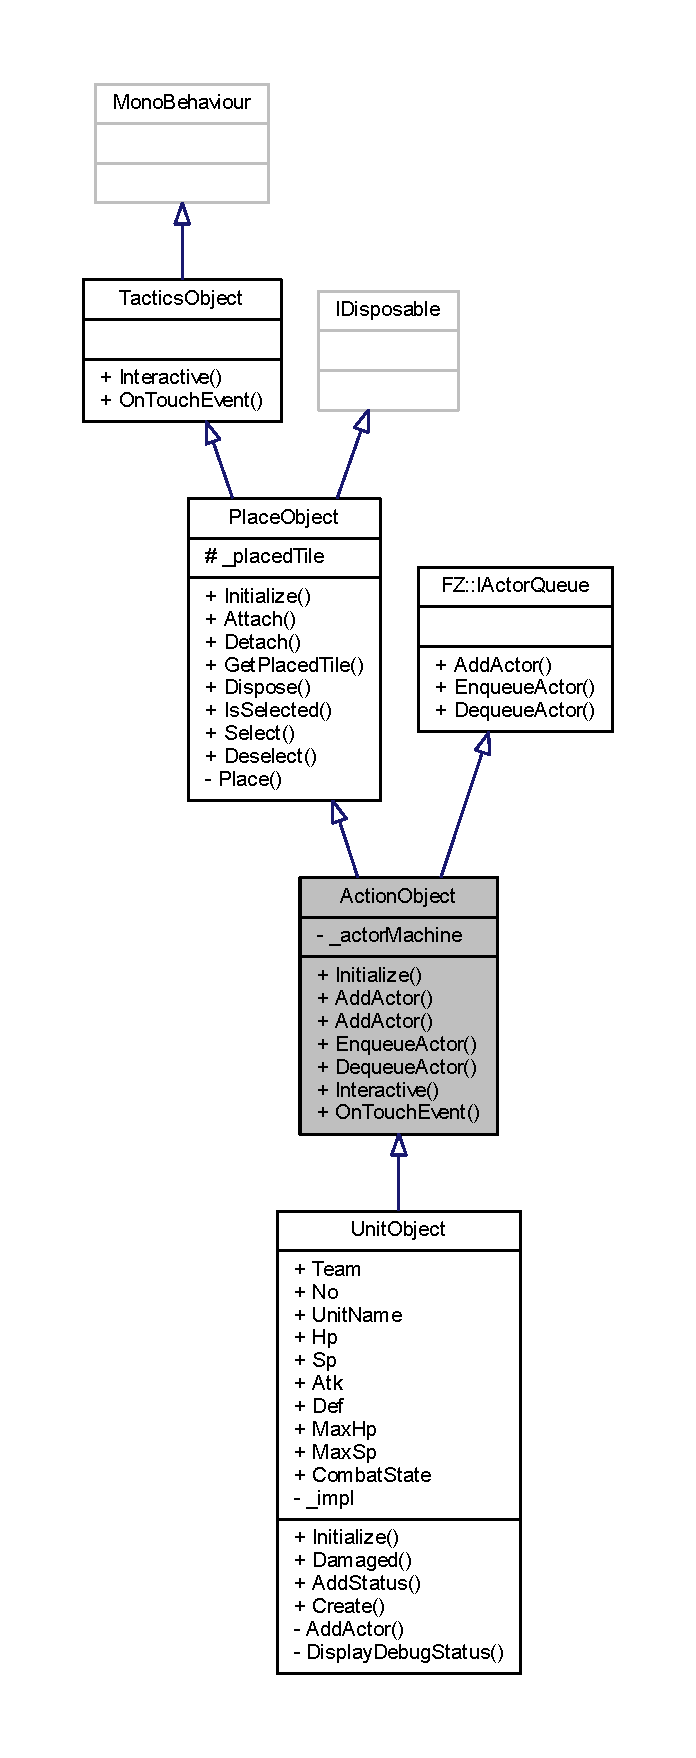
\includegraphics[height=550pt]{class_action_object__inherit__graph}
\end{center}
\end{figure}


Action\+Object에 대한 협력 다이어그램\+:
\nopagebreak
\begin{figure}[H]
\begin{center}
\leavevmode
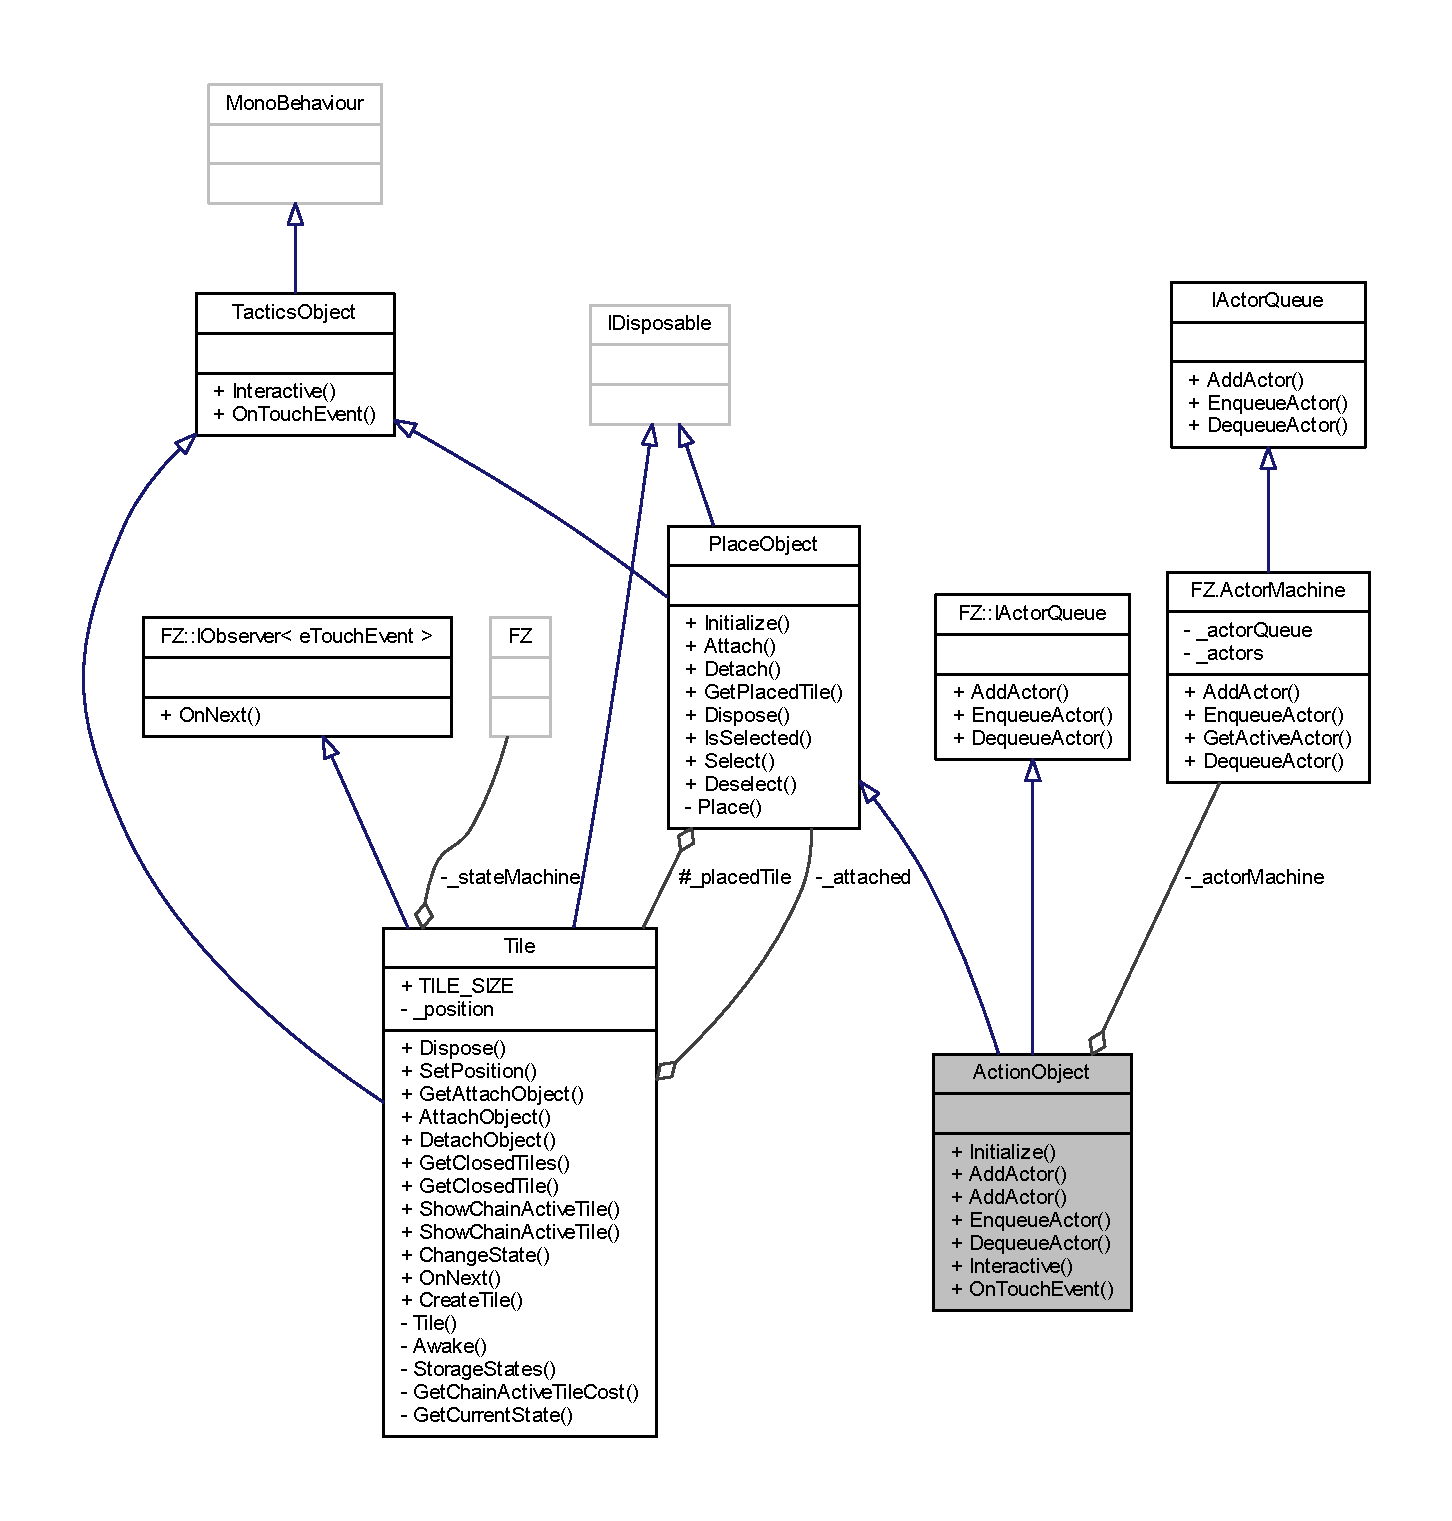
\includegraphics[width=350pt]{class_action_object__coll__graph}
\end{center}
\end{figure}
\subsection*{Public 멤버 함수}
\begin{DoxyCompactItemize}
\item 
override void \hyperlink{class_action_object_afe93413cd4bfad308b8c357b4fd9dc30}{Initialize} (\hyperlink{class_data_object}{Data\+Object} data)
\item 
void \hyperlink{class_action_object_a56caea069fa424581114bd41b299944c}{Add\+Actor} (\hyperlink{class_f_z_1_1_actor}{Actor} actor)
\item 
void \hyperlink{class_action_object_a25c60d577ecf4dedb7d5af668fe1c8e7}{Add\+Actor} (\hyperlink{class_actor_info}{Actor\+Info} info)
\item 
void \hyperlink{class_action_object_a1aa21a0bbc88cf7456dd20005d55e972}{Enqueue\+Actor} (Type actor\+Type)
\item 
void \hyperlink{class_action_object_a57bca80c5d001408121c21ee46422976}{Dequeue\+Actor} ()
\item 
override void \hyperlink{class_action_object_a82d2b5b3c03a27d913df32d2bb9e8406}{Interactive} (\hyperlink{class_tactics_object}{Tactics\+Object} interact\+Target)
\item 
override bool \hyperlink{class_action_object_a0f3ad33fd4ec0478fbe397aaa92c257e}{On\+Touch\+Event} (\hyperlink{_touch_manager_8cs_ae33e321a424fe84ba8b2fdb81ad40a68}{e\+Touch\+Event} touch)
\item 
void \hyperlink{class_place_object_aa0f1a877d0abc20133e390d0964602ed}{Attach} (\hyperlink{class_tile}{Tile} tile)
\item 
void \hyperlink{class_place_object_a5bcf3ff3fd935121fbd699a08da217e2}{Detach} ()
\item 
\hyperlink{class_tile}{Tile} \hyperlink{class_place_object_a55363002bd68063cf079185a5729b76c}{Get\+Placed\+Tile} ()
\item 
void \hyperlink{class_place_object_aeac9db9685cc3134a90b6a2578046933}{Dispose} ()
\item 
bool \hyperlink{class_place_object_a55fd3f2bd6cccd98390c675371ab723e}{Is\+Selected} ()
\item 
void \hyperlink{class_place_object_a76b1b569fa2aa204ee8e2cb6a350694d}{Select} ()
\item 
void \hyperlink{class_place_object_ad54985fa9ccaf2df149af83b4f17892e}{Deselect} ()
\item 
void \hyperlink{interface_f_z_1_1_i_actor_queue_a913b199f922223b26cf05efa96c14139}{Add\+Actor} (\hyperlink{class_f_z_1_1_actor}{F\+Z.\+Actor} actor)
\item 
void \hyperlink{interface_f_z_1_1_i_actor_queue_ad0ffa88154fd9f44e0a8828b31a10c03}{Enqueue\+Actor} (System.\+Type actor\+Type)
\end{DoxyCompactItemize}
\subsection*{Protected 속성}
\begin{DoxyCompactItemize}
\item 
\hyperlink{class_tile}{Tile} \hyperlink{class_place_object_a2006d9f7ffcf8aba6f731ebfc9b0af35}{\+\_\+placed\+Tile}
\end{DoxyCompactItemize}
\subsection*{Private 속성}
\begin{DoxyCompactItemize}
\item 
\hyperlink{class_f_z_1_1_actor_machine}{Actor\+Machine} \hyperlink{class_action_object_a099f059d9ecf46cbf1a7d9e6fb035e03}{\+\_\+actor\+Machine} = new \hyperlink{class_f_z_1_1_actor_machine}{Actor\+Machine}()
\end{DoxyCompactItemize}


\subsection{상세한 설명}


Action\+Object.\+cs 파일의 7 번째 라인에서 정의되었습니다.



\subsection{멤버 함수 문서화}
\index{Action\+Object@{Action\+Object}!Add\+Actor@{Add\+Actor}}
\index{Add\+Actor@{Add\+Actor}!Action\+Object@{Action\+Object}}
\subsubsection[{\texorpdfstring{Add\+Actor(\+F\+Z.\+Actor actor)}{AddActor(FZ.Actor actor)}}]{\setlength{\rightskip}{0pt plus 5cm}void F\+Z.\+I\+Actor\+Queue.\+Add\+Actor (
\begin{DoxyParamCaption}
\item[{{\bf F\+Z.\+Actor}}]{actor}
\end{DoxyParamCaption}
)\hspace{0.3cm}{\ttfamily [inherited]}}\hypertarget{interface_f_z_1_1_i_actor_queue_a913b199f922223b26cf05efa96c14139}{}\label{interface_f_z_1_1_i_actor_queue_a913b199f922223b26cf05efa96c14139}


\hyperlink{class_f_z_1_1_actor_machine_abf6949bf5213c6b7eb9f7b2d0c677a23}{F\+Z.\+Actor\+Machine}에서 구현되었습니다.

\index{Action\+Object@{Action\+Object}!Add\+Actor@{Add\+Actor}}
\index{Add\+Actor@{Add\+Actor}!Action\+Object@{Action\+Object}}
\subsubsection[{\texorpdfstring{Add\+Actor(\+Actor actor)}{AddActor(Actor actor)}}]{\setlength{\rightskip}{0pt plus 5cm}void Action\+Object.\+Add\+Actor (
\begin{DoxyParamCaption}
\item[{{\bf Actor}}]{actor}
\end{DoxyParamCaption}
)}\hypertarget{class_action_object_a56caea069fa424581114bd41b299944c}{}\label{class_action_object_a56caea069fa424581114bd41b299944c}


Action\+Object.\+cs 파일의 22 번째 라인에서 정의되었습니다.


\begin{DoxyCode}
23     \{
24         \hyperlink{class_action_object_a099f059d9ecf46cbf1a7d9e6fb035e03}{\_actorMachine}.\hyperlink{class_f_z_1_1_actor_machine_abf6949bf5213c6b7eb9f7b2d0c677a23}{AddActor}(actor);
25     \}
\end{DoxyCode}


이 함수 내부에서 호출하는 함수들에 대한 그래프입니다.\+:
\nopagebreak
\begin{figure}[H]
\begin{center}
\leavevmode
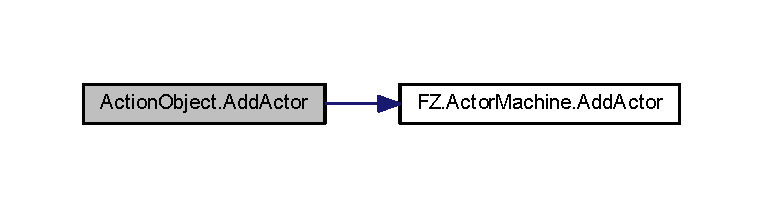
\includegraphics[width=350pt]{class_action_object_a56caea069fa424581114bd41b299944c_cgraph}
\end{center}
\end{figure}




이 함수를 호출하는 함수들에 대한 그래프입니다.\+:
\nopagebreak
\begin{figure}[H]
\begin{center}
\leavevmode
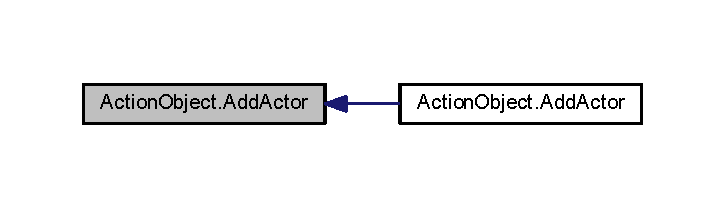
\includegraphics[width=348pt]{class_action_object_a56caea069fa424581114bd41b299944c_icgraph}
\end{center}
\end{figure}


\index{Action\+Object@{Action\+Object}!Add\+Actor@{Add\+Actor}}
\index{Add\+Actor@{Add\+Actor}!Action\+Object@{Action\+Object}}
\subsubsection[{\texorpdfstring{Add\+Actor(\+Actor\+Info info)}{AddActor(ActorInfo info)}}]{\setlength{\rightskip}{0pt plus 5cm}void Action\+Object.\+Add\+Actor (
\begin{DoxyParamCaption}
\item[{{\bf Actor\+Info}}]{info}
\end{DoxyParamCaption}
)}\hypertarget{class_action_object_a25c60d577ecf4dedb7d5af668fe1c8e7}{}\label{class_action_object_a25c60d577ecf4dedb7d5af668fe1c8e7}


Action\+Object.\+cs 파일의 27 번째 라인에서 정의되었습니다.


\begin{DoxyCode}
28     \{
29         Assembly assembly = Assembly.GetExecutingAssembly();
30         \textcolor{keywordflow}{try}
31         \{
32             Type actorType = assembly.GetType(info.\hyperlink{class_actor_info_a2e9e540cdc037f204d80622e47543410}{name});
33 
34             \hyperlink{namespace_f_z}{FZ}.\hyperlink{class_f_z_1_1_actor}{Actor} actor = (\hyperlink{namespace_f_z}{FZ}.\hyperlink{class_f_z_1_1_actor}{Actor})Activator.CreateInstance(actorType);
35 
36             \textcolor{keywordflow}{if} (actor != null)
37             \{
38                 actor.\hyperlink{class_f_z_1_1_actor_ac29de02b4c3cc1012143f6531f5809ed}{Initialize}(\textcolor{keyword}{this}, info.\hyperlink{class_actor_info_a25bb8e0eafab630572ffddea088a1f80}{weightName}, info.
      \hyperlink{class_actor_info_a1c5dd2d46e5ebc5a6483f2bcb55cb162}{weightValue});
39             \}
40 
41             this.\hyperlink{class_action_object_a56caea069fa424581114bd41b299944c}{AddActor}(actor);
42 
43 \textcolor{preprocessor}{#if UNITY\_EDITOR}
44             \textcolor{comment}{// 이건 디버깅용으로.. 무조껀 큐에 삽입한다.}
45             this.\hyperlink{class_action_object_a1aa21a0bbc88cf7456dd20005d55e972}{EnqueueActor}(actor.GetType());
46 \textcolor{preprocessor}{#endif}
47         \}
48         \textcolor{keywordflow}{catch} (Exception e)
49         \{
50             \textcolor{keywordflow}{throw} \textcolor{keyword}{new} UnityException(e.ToString());
51         \}
52     \}
\end{DoxyCode}


이 함수 내부에서 호출하는 함수들에 대한 그래프입니다.\+:
\nopagebreak
\begin{figure}[H]
\begin{center}
\leavevmode
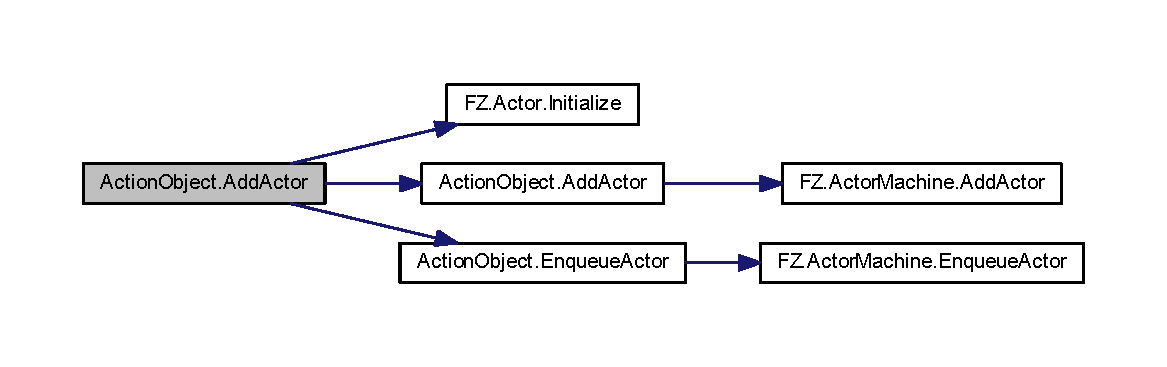
\includegraphics[width=350pt]{class_action_object_a25c60d577ecf4dedb7d5af668fe1c8e7_cgraph}
\end{center}
\end{figure}


\index{Action\+Object@{Action\+Object}!Attach@{Attach}}
\index{Attach@{Attach}!Action\+Object@{Action\+Object}}
\subsubsection[{\texorpdfstring{Attach(\+Tile tile)}{Attach(Tile tile)}}]{\setlength{\rightskip}{0pt plus 5cm}void Place\+Object.\+Attach (
\begin{DoxyParamCaption}
\item[{{\bf Tile}}]{tile}
\end{DoxyParamCaption}
)\hspace{0.3cm}{\ttfamily [inherited]}}\hypertarget{class_place_object_aa0f1a877d0abc20133e390d0964602ed}{}\label{class_place_object_aa0f1a877d0abc20133e390d0964602ed}


Place\+Object.\+cs 파일의 19 번째 라인에서 정의되었습니다.


\begin{DoxyCode}
20     \{
21         \textcolor{comment}{// 순환 참조 적용. 레퍼런스 관리에 신경 쓸 것}
22         \hyperlink{class_place_object_a2006d9f7ffcf8aba6f731ebfc9b0af35}{\_placedTile} = tile;
23 
24         \hyperlink{class_place_object_aee28273784ccccbc9df57c6bddead3fd}{Place}(tile);
25     \}
\end{DoxyCode}


이 함수 내부에서 호출하는 함수들에 대한 그래프입니다.\+:
\nopagebreak
\begin{figure}[H]
\begin{center}
\leavevmode
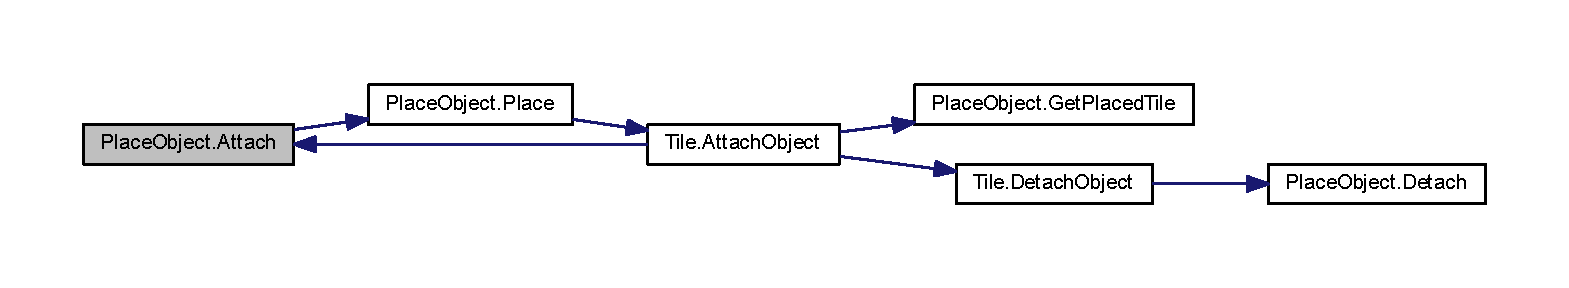
\includegraphics[width=350pt]{class_place_object_aa0f1a877d0abc20133e390d0964602ed_cgraph}
\end{center}
\end{figure}




이 함수를 호출하는 함수들에 대한 그래프입니다.\+:
\nopagebreak
\begin{figure}[H]
\begin{center}
\leavevmode
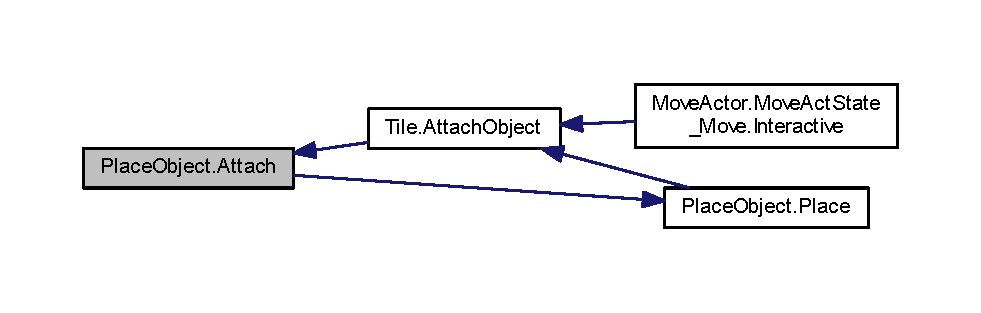
\includegraphics[width=350pt]{class_place_object_aa0f1a877d0abc20133e390d0964602ed_icgraph}
\end{center}
\end{figure}


\index{Action\+Object@{Action\+Object}!Dequeue\+Actor@{Dequeue\+Actor}}
\index{Dequeue\+Actor@{Dequeue\+Actor}!Action\+Object@{Action\+Object}}
\subsubsection[{\texorpdfstring{Dequeue\+Actor()}{DequeueActor()}}]{\setlength{\rightskip}{0pt plus 5cm}void Action\+Object.\+Dequeue\+Actor (
\begin{DoxyParamCaption}
{}
\end{DoxyParamCaption}
)}\hypertarget{class_action_object_a57bca80c5d001408121c21ee46422976}{}\label{class_action_object_a57bca80c5d001408121c21ee46422976}


\hyperlink{interface_f_z_1_1_i_actor_queue_a4299dfbeb2b3296677ccfc02fe0eaad7}{F\+Z.\+I\+Actor\+Queue}를 구현.



Action\+Object.\+cs 파일의 63 번째 라인에서 정의되었습니다.


\begin{DoxyCode}
64     \{
65         \hyperlink{class_action_object_a099f059d9ecf46cbf1a7d9e6fb035e03}{\_actorMachine}.\hyperlink{class_f_z_1_1_actor_machine_a469fc3e9b02b02a2a8efb3e4c1e4101d}{DequeueActor}();
66 
67 \textcolor{preprocessor}{#if UNITY\_EDITOR}
68         \_actorDebugQueue.RemoveAt(0);
69 \textcolor{preprocessor}{#endif}
70     \}
\end{DoxyCode}


이 함수 내부에서 호출하는 함수들에 대한 그래프입니다.\+:
\nopagebreak
\begin{figure}[H]
\begin{center}
\leavevmode
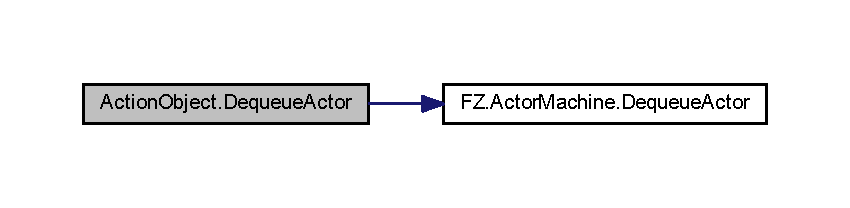
\includegraphics[width=350pt]{class_action_object_a57bca80c5d001408121c21ee46422976_cgraph}
\end{center}
\end{figure}


\index{Action\+Object@{Action\+Object}!Deselect@{Deselect}}
\index{Deselect@{Deselect}!Action\+Object@{Action\+Object}}
\subsubsection[{\texorpdfstring{Deselect()}{Deselect()}}]{\setlength{\rightskip}{0pt plus 5cm}void Place\+Object.\+Deselect (
\begin{DoxyParamCaption}
{}
\end{DoxyParamCaption}
)\hspace{0.3cm}{\ttfamily [inherited]}}\hypertarget{class_place_object_ad54985fa9ccaf2df149af83b4f17892e}{}\label{class_place_object_ad54985fa9ccaf2df149af83b4f17892e}


Place\+Object.\+cs 파일의 67 번째 라인에서 정의되었습니다.


\begin{DoxyCode}
68     \{
69         \hyperlink{class_game_manager}{GameManager}.\hyperlink{class_f_z_1_1_singletone_a8e7ba3cf5cff48b1101428beefcd76b4}{Instance}.SelectedObj = null;
70     \}
\end{DoxyCode}
\index{Action\+Object@{Action\+Object}!Detach@{Detach}}
\index{Detach@{Detach}!Action\+Object@{Action\+Object}}
\subsubsection[{\texorpdfstring{Detach()}{Detach()}}]{\setlength{\rightskip}{0pt plus 5cm}void Place\+Object.\+Detach (
\begin{DoxyParamCaption}
{}
\end{DoxyParamCaption}
)\hspace{0.3cm}{\ttfamily [inherited]}}\hypertarget{class_place_object_a5bcf3ff3fd935121fbd699a08da217e2}{}\label{class_place_object_a5bcf3ff3fd935121fbd699a08da217e2}


Place\+Object.\+cs 파일의 29 번째 라인에서 정의되었습니다.


\begin{DoxyCode}
30     \{
31         \hyperlink{class_place_object_a2006d9f7ffcf8aba6f731ebfc9b0af35}{\_placedTile} = null;
32     \}
\end{DoxyCode}


이 함수를 호출하는 함수들에 대한 그래프입니다.\+:
\nopagebreak
\begin{figure}[H]
\begin{center}
\leavevmode
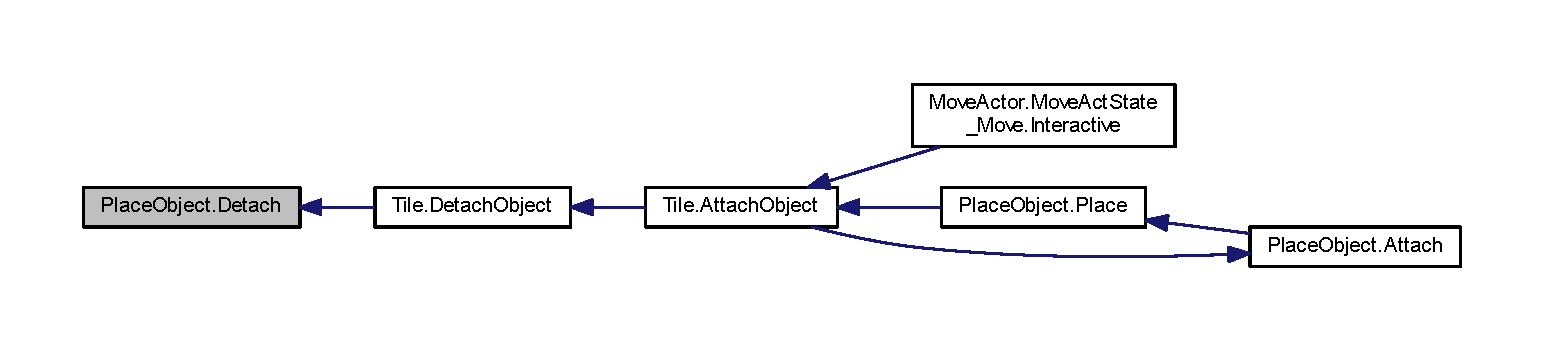
\includegraphics[width=350pt]{class_place_object_a5bcf3ff3fd935121fbd699a08da217e2_icgraph}
\end{center}
\end{figure}


\index{Action\+Object@{Action\+Object}!Dispose@{Dispose}}
\index{Dispose@{Dispose}!Action\+Object@{Action\+Object}}
\subsubsection[{\texorpdfstring{Dispose()}{Dispose()}}]{\setlength{\rightskip}{0pt plus 5cm}void Place\+Object.\+Dispose (
\begin{DoxyParamCaption}
{}
\end{DoxyParamCaption}
)\hspace{0.3cm}{\ttfamily [inherited]}}\hypertarget{class_place_object_aeac9db9685cc3134a90b6a2578046933}{}\label{class_place_object_aeac9db9685cc3134a90b6a2578046933}


Place\+Object.\+cs 파일의 39 번째 라인에서 정의되었습니다.


\begin{DoxyCode}
40     \{
41         \hyperlink{class_place_object_a2006d9f7ffcf8aba6f731ebfc9b0af35}{\_placedTile} = null;
42 
43         GameObject.Destroy(gameObject);
44     \}
\end{DoxyCode}


이 함수를 호출하는 함수들에 대한 그래프입니다.\+:
\nopagebreak
\begin{figure}[H]
\begin{center}
\leavevmode
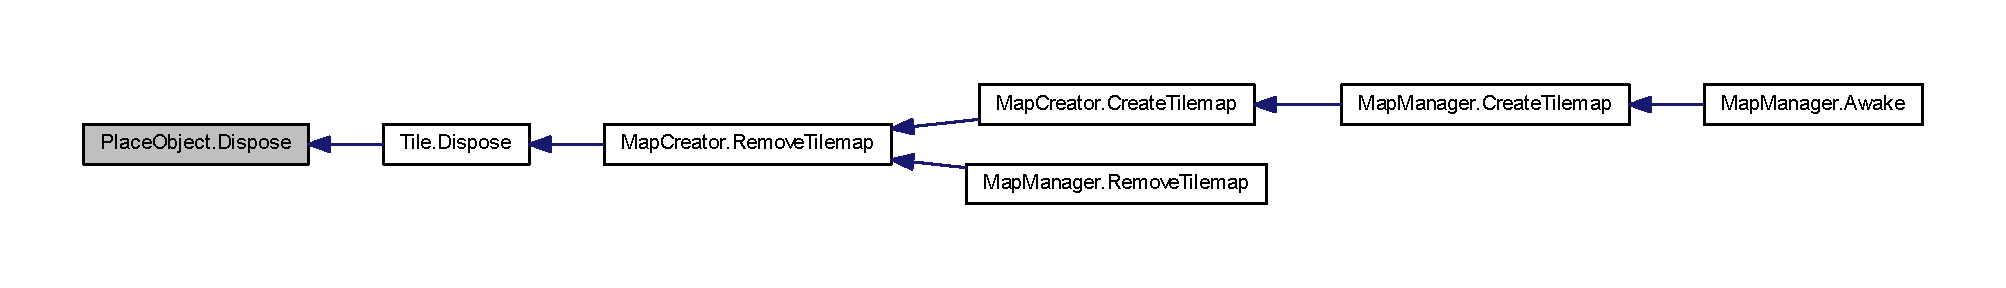
\includegraphics[width=350pt]{class_place_object_aeac9db9685cc3134a90b6a2578046933_icgraph}
\end{center}
\end{figure}


\index{Action\+Object@{Action\+Object}!Enqueue\+Actor@{Enqueue\+Actor}}
\index{Enqueue\+Actor@{Enqueue\+Actor}!Action\+Object@{Action\+Object}}
\subsubsection[{\texorpdfstring{Enqueue\+Actor(\+System.\+Type actor\+Type)}{EnqueueActor(System.Type actorType)}}]{\setlength{\rightskip}{0pt plus 5cm}void F\+Z.\+I\+Actor\+Queue.\+Enqueue\+Actor (
\begin{DoxyParamCaption}
\item[{System.\+Type}]{actor\+Type}
\end{DoxyParamCaption}
)\hspace{0.3cm}{\ttfamily [inherited]}}\hypertarget{interface_f_z_1_1_i_actor_queue_ad0ffa88154fd9f44e0a8828b31a10c03}{}\label{interface_f_z_1_1_i_actor_queue_ad0ffa88154fd9f44e0a8828b31a10c03}


\hyperlink{class_f_z_1_1_actor_machine_ac399a880001dbecdc39c1807f81e4eac}{F\+Z.\+Actor\+Machine}에서 구현되었습니다.

\index{Action\+Object@{Action\+Object}!Enqueue\+Actor@{Enqueue\+Actor}}
\index{Enqueue\+Actor@{Enqueue\+Actor}!Action\+Object@{Action\+Object}}
\subsubsection[{\texorpdfstring{Enqueue\+Actor(\+Type actor\+Type)}{EnqueueActor(Type actorType)}}]{\setlength{\rightskip}{0pt plus 5cm}void Action\+Object.\+Enqueue\+Actor (
\begin{DoxyParamCaption}
\item[{Type}]{actor\+Type}
\end{DoxyParamCaption}
)}\hypertarget{class_action_object_a1aa21a0bbc88cf7456dd20005d55e972}{}\label{class_action_object_a1aa21a0bbc88cf7456dd20005d55e972}


Action\+Object.\+cs 파일의 54 번째 라인에서 정의되었습니다.


\begin{DoxyCode}
55     \{
56         \hyperlink{class_action_object_a099f059d9ecf46cbf1a7d9e6fb035e03}{\_actorMachine}.\hyperlink{class_f_z_1_1_actor_machine_ac399a880001dbecdc39c1807f81e4eac}{EnqueueActor}(actorType);
57 
58 \textcolor{preprocessor}{#if UNITY\_EDITOR}
59         \_actorDebugQueue.Add(actorType.ToString());
60 \textcolor{preprocessor}{#endif}
61     \}
\end{DoxyCode}


이 함수 내부에서 호출하는 함수들에 대한 그래프입니다.\+:
\nopagebreak
\begin{figure}[H]
\begin{center}
\leavevmode
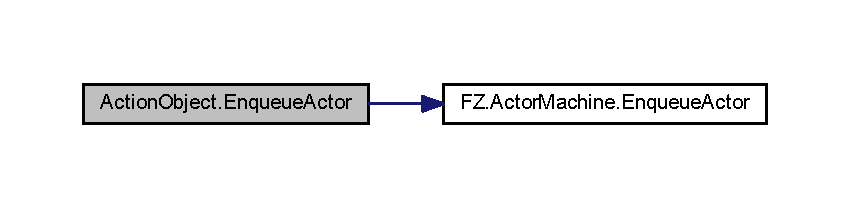
\includegraphics[width=350pt]{class_action_object_a1aa21a0bbc88cf7456dd20005d55e972_cgraph}
\end{center}
\end{figure}




이 함수를 호출하는 함수들에 대한 그래프입니다.\+:
\nopagebreak
\begin{figure}[H]
\begin{center}
\leavevmode
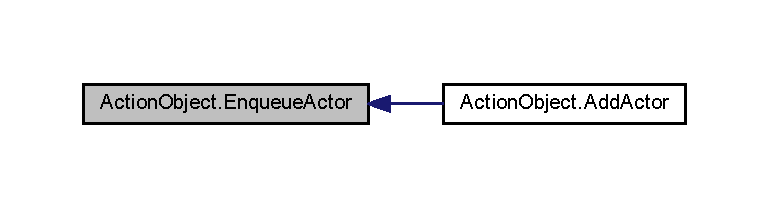
\includegraphics[width=350pt]{class_action_object_a1aa21a0bbc88cf7456dd20005d55e972_icgraph}
\end{center}
\end{figure}


\index{Action\+Object@{Action\+Object}!Get\+Placed\+Tile@{Get\+Placed\+Tile}}
\index{Get\+Placed\+Tile@{Get\+Placed\+Tile}!Action\+Object@{Action\+Object}}
\subsubsection[{\texorpdfstring{Get\+Placed\+Tile()}{GetPlacedTile()}}]{\setlength{\rightskip}{0pt plus 5cm}{\bf Tile} Place\+Object.\+Get\+Placed\+Tile (
\begin{DoxyParamCaption}
{}
\end{DoxyParamCaption}
)\hspace{0.3cm}{\ttfamily [inherited]}}\hypertarget{class_place_object_a55363002bd68063cf079185a5729b76c}{}\label{class_place_object_a55363002bd68063cf079185a5729b76c}


Place\+Object.\+cs 파일의 34 번째 라인에서 정의되었습니다.


\begin{DoxyCode}
35     \{
36         \textcolor{keywordflow}{return} \hyperlink{class_place_object_a2006d9f7ffcf8aba6f731ebfc9b0af35}{\_placedTile};
37     \}
\end{DoxyCode}


이 함수를 호출하는 함수들에 대한 그래프입니다.\+:
\nopagebreak
\begin{figure}[H]
\begin{center}
\leavevmode
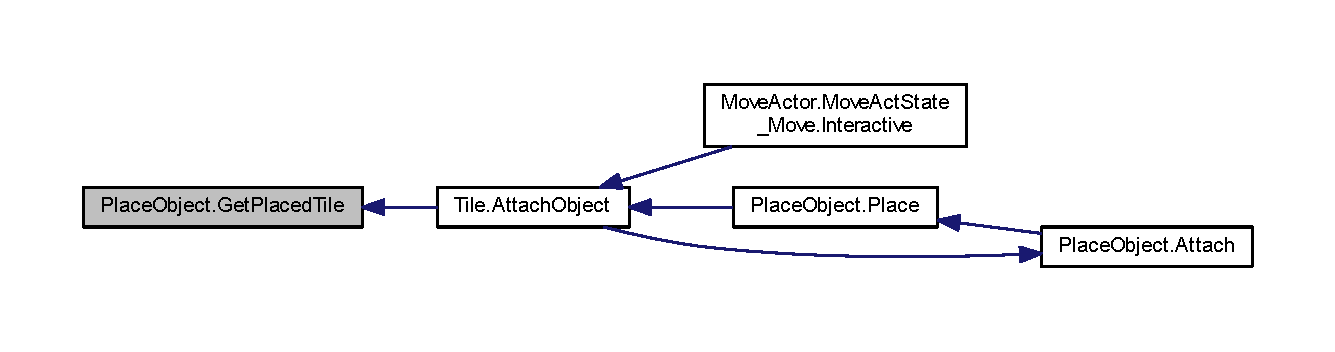
\includegraphics[width=350pt]{class_place_object_a55363002bd68063cf079185a5729b76c_icgraph}
\end{center}
\end{figure}


\index{Action\+Object@{Action\+Object}!Initialize@{Initialize}}
\index{Initialize@{Initialize}!Action\+Object@{Action\+Object}}
\subsubsection[{\texorpdfstring{Initialize(\+Data\+Object data)}{Initialize(DataObject data)}}]{\setlength{\rightskip}{0pt plus 5cm}override void Action\+Object.\+Initialize (
\begin{DoxyParamCaption}
\item[{{\bf Data\+Object}}]{data}
\end{DoxyParamCaption}
)\hspace{0.3cm}{\ttfamily [virtual]}}\hypertarget{class_action_object_afe93413cd4bfad308b8c357b4fd9dc30}{}\label{class_action_object_afe93413cd4bfad308b8c357b4fd9dc30}


\hyperlink{class_place_object_a57f8bb8f58e18a673e3114a8227697db}{Place\+Object}(으)로부터 재구현되었습니다.



\hyperlink{class_unit_object_acc70df752878272e4f9d0f0dc1f68f84}{Unit\+Object}에서 재구현되었습니다.



Action\+Object.\+cs 파일의 17 번째 라인에서 정의되었습니다.


\begin{DoxyCode}
18     \{
19 
20     \}
\end{DoxyCode}
\index{Action\+Object@{Action\+Object}!Interactive@{Interactive}}
\index{Interactive@{Interactive}!Action\+Object@{Action\+Object}}
\subsubsection[{\texorpdfstring{Interactive(\+Tactics\+Object interact\+Target)}{Interactive(TacticsObject interactTarget)}}]{\setlength{\rightskip}{0pt plus 5cm}override void Action\+Object.\+Interactive (
\begin{DoxyParamCaption}
\item[{{\bf Tactics\+Object}}]{interact\+Target}
\end{DoxyParamCaption}
)\hspace{0.3cm}{\ttfamily [virtual]}}\hypertarget{class_action_object_a82d2b5b3c03a27d913df32d2bb9e8406}{}\label{class_action_object_a82d2b5b3c03a27d913df32d2bb9e8406}


\hyperlink{class_tactics_object_a5f94ed01497a7072a2785163f4cbc57b}{Tactics\+Object}(으)로부터 재구현되었습니다.



Action\+Object.\+cs 파일의 73 번째 라인에서 정의되었습니다.


\begin{DoxyCode}
74     \{
75         var activeActor = \hyperlink{class_action_object_a099f059d9ecf46cbf1a7d9e6fb035e03}{\_actorMachine}.\hyperlink{class_f_z_1_1_actor_machine_a9f1efcf25b000d4634abcc97d361c629}{GetActiveActor}();
76         \textcolor{keywordflow}{if} (activeActor != null)
77         \{
78             activeActor.\hyperlink{class_f_z_1_1_actor_a1d5780d31a35893d38598d78c8f0c74a}{Interactive}(interactTarget);
79         \}
80     \}
\end{DoxyCode}


이 함수 내부에서 호출하는 함수들에 대한 그래프입니다.\+:
\nopagebreak
\begin{figure}[H]
\begin{center}
\leavevmode
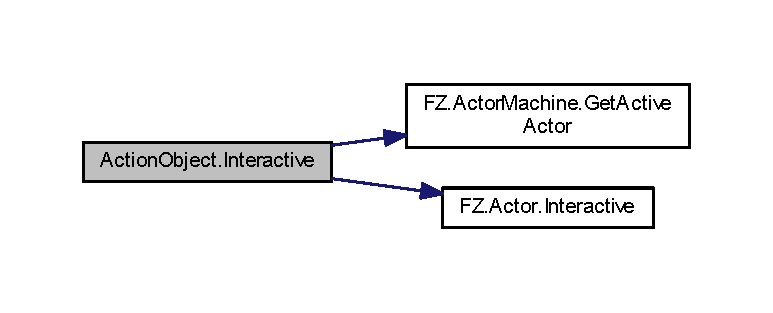
\includegraphics[width=350pt]{class_action_object_a82d2b5b3c03a27d913df32d2bb9e8406_cgraph}
\end{center}
\end{figure}


\index{Action\+Object@{Action\+Object}!Is\+Selected@{Is\+Selected}}
\index{Is\+Selected@{Is\+Selected}!Action\+Object@{Action\+Object}}
\subsubsection[{\texorpdfstring{Is\+Selected()}{IsSelected()}}]{\setlength{\rightskip}{0pt plus 5cm}bool Place\+Object.\+Is\+Selected (
\begin{DoxyParamCaption}
{}
\end{DoxyParamCaption}
)\hspace{0.3cm}{\ttfamily [inherited]}}\hypertarget{class_place_object_a55fd3f2bd6cccd98390c675371ab723e}{}\label{class_place_object_a55fd3f2bd6cccd98390c675371ab723e}


Place\+Object.\+cs 파일의 57 번째 라인에서 정의되었습니다.


\begin{DoxyCode}
58     \{
59         \textcolor{keywordflow}{return} \hyperlink{class_game_manager}{GameManager}.\hyperlink{class_f_z_1_1_singletone_a8e7ba3cf5cff48b1101428beefcd76b4}{Instance}.SelectedObj == \textcolor{keyword}{this};
60     \}
\end{DoxyCode}
\index{Action\+Object@{Action\+Object}!On\+Touch\+Event@{On\+Touch\+Event}}
\index{On\+Touch\+Event@{On\+Touch\+Event}!Action\+Object@{Action\+Object}}
\subsubsection[{\texorpdfstring{On\+Touch\+Event(e\+Touch\+Event touch)}{OnTouchEvent(eTouchEvent touch)}}]{\setlength{\rightskip}{0pt plus 5cm}override bool Action\+Object.\+On\+Touch\+Event (
\begin{DoxyParamCaption}
\item[{{\bf e\+Touch\+Event}}]{touch}
\end{DoxyParamCaption}
)\hspace{0.3cm}{\ttfamily [virtual]}}\hypertarget{class_action_object_a0f3ad33fd4ec0478fbe397aaa92c257e}{}\label{class_action_object_a0f3ad33fd4ec0478fbe397aaa92c257e}


\hyperlink{class_tactics_object_af34052e62ea471d21e4c601cc79ff717}{Tactics\+Object}(으)로부터 재구현되었습니다.



Action\+Object.\+cs 파일의 82 번째 라인에서 정의되었습니다.


\begin{DoxyCode}
83     \{
84         var activeActor = \hyperlink{class_action_object_a099f059d9ecf46cbf1a7d9e6fb035e03}{\_actorMachine}.\hyperlink{class_f_z_1_1_actor_machine_a9f1efcf25b000d4634abcc97d361c629}{GetActiveActor}();
85         \textcolor{keywordflow}{if} (activeActor != null)
86         \{
87             activeActor.\hyperlink{class_f_z_1_1_actor_a9f30b12f3615a447df054d48ef4e22c7}{OnTouchEvent}(touch);
88         \}
89 
90         \textcolor{keywordflow}{return} \textcolor{keyword}{true};
91     \}
\end{DoxyCode}


이 함수 내부에서 호출하는 함수들에 대한 그래프입니다.\+:
\nopagebreak
\begin{figure}[H]
\begin{center}
\leavevmode
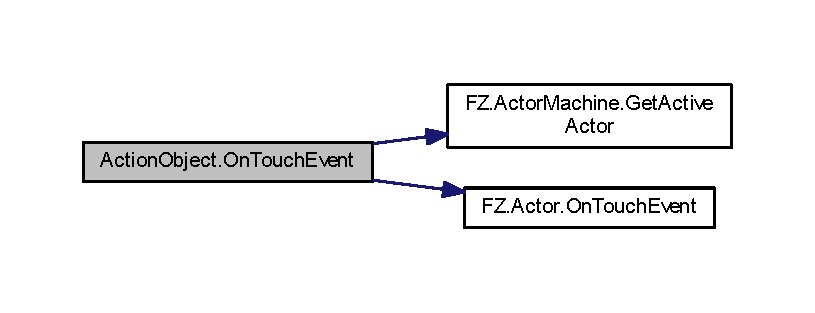
\includegraphics[width=350pt]{class_action_object_a0f3ad33fd4ec0478fbe397aaa92c257e_cgraph}
\end{center}
\end{figure}


\index{Action\+Object@{Action\+Object}!Select@{Select}}
\index{Select@{Select}!Action\+Object@{Action\+Object}}
\subsubsection[{\texorpdfstring{Select()}{Select()}}]{\setlength{\rightskip}{0pt plus 5cm}void Place\+Object.\+Select (
\begin{DoxyParamCaption}
{}
\end{DoxyParamCaption}
)\hspace{0.3cm}{\ttfamily [inherited]}}\hypertarget{class_place_object_a76b1b569fa2aa204ee8e2cb6a350694d}{}\label{class_place_object_a76b1b569fa2aa204ee8e2cb6a350694d}


Place\+Object.\+cs 파일의 62 번째 라인에서 정의되었습니다.


\begin{DoxyCode}
63     \{
64         \hyperlink{class_game_manager}{GameManager}.\hyperlink{class_f_z_1_1_singletone_a8e7ba3cf5cff48b1101428beefcd76b4}{Instance}.SelectedObj = \textcolor{keyword}{this};
65     \}
\end{DoxyCode}


\subsection{멤버 데이타 문서화}
\index{Action\+Object@{Action\+Object}!\+\_\+actor\+Machine@{\+\_\+actor\+Machine}}
\index{\+\_\+actor\+Machine@{\+\_\+actor\+Machine}!Action\+Object@{Action\+Object}}
\subsubsection[{\texorpdfstring{\+\_\+actor\+Machine}{_actorMachine}}]{\setlength{\rightskip}{0pt plus 5cm}{\bf Actor\+Machine} Action\+Object.\+\_\+actor\+Machine = new {\bf Actor\+Machine}()\hspace{0.3cm}{\ttfamily [private]}}\hypertarget{class_action_object_a099f059d9ecf46cbf1a7d9e6fb035e03}{}\label{class_action_object_a099f059d9ecf46cbf1a7d9e6fb035e03}


Action\+Object.\+cs 파일의 9 번째 라인에서 정의되었습니다.

\index{Action\+Object@{Action\+Object}!\+\_\+placed\+Tile@{\+\_\+placed\+Tile}}
\index{\+\_\+placed\+Tile@{\+\_\+placed\+Tile}!Action\+Object@{Action\+Object}}
\subsubsection[{\texorpdfstring{\+\_\+placed\+Tile}{_placedTile}}]{\setlength{\rightskip}{0pt plus 5cm}{\bf Tile} Place\+Object.\+\_\+placed\+Tile\hspace{0.3cm}{\ttfamily [protected]}, {\ttfamily [inherited]}}\hypertarget{class_place_object_a2006d9f7ffcf8aba6f731ebfc9b0af35}{}\label{class_place_object_a2006d9f7ffcf8aba6f731ebfc9b0af35}


Place\+Object.\+cs 파일의 10 번째 라인에서 정의되었습니다.



이 클래스에 대한 문서화 페이지는 다음의 파일로부터 생성되었습니다.\+:\begin{DoxyCompactItemize}
\item 
D\+:/\+Git\+Hub/\+M\+C\+N\+Tactics/\+Assets/\+Scripts/\+Objects/\hyperlink{_action_object_8cs}{Action\+Object.\+cs}\end{DoxyCompactItemize}

\hypertarget{class_f_z_1_1_act_obj_actor}{}\section{F\+Z.\+Act\+Obj\+Actor 클래스 참조}
\label{class_f_z_1_1_act_obj_actor}\index{F\+Z.\+Act\+Obj\+Actor@{F\+Z.\+Act\+Obj\+Actor}}


F\+Z.\+Act\+Obj\+Actor에 대한 상속 다이어그램 \+: 
% FIG 0


F\+Z.\+Act\+Obj\+Actor에 대한 협력 다이어그램\+:
% FIG 1
\subsection*{Public 멤버 함수}
\begin{DoxyCompactItemize}
\item 
bool \hyperlink{class_f_z_1_1_actor_aa78fa8d765cfc56474c3714d38bcc13b}{Check\+Absolute\+Weight\+Key} ()
\item 
void \hyperlink{class_f_z_1_1_actor_ac29de02b4c3cc1012143f6531f5809ed}{Initialize} (\hyperlink{interface_f_z_1_1_i_actor_queue}{I\+Actor\+Queue} act\+Target, List$<$ \hyperlink{class_f_z_1_1_string_int_pair}{String\+Int\+Pair} $>$ weights)
\item 
void \hyperlink{class_f_z_1_1_actor_a968a8b42fa52f121bdcc9c8ea8136eb9}{Initialize} (\hyperlink{interface_f_z_1_1_i_actor_queue}{I\+Actor\+Queue} act\+Target, List$<$ string $>$ weight\+Name, List$<$ int $>$ weight\+Value)
\item 
int \hyperlink{class_f_z_1_1_actor_ab6dee08c1296f3c020694fd9408b7c33}{Get\+Weight} (string key)
\item 
void \hyperlink{class_f_z_1_1_actor_a0f36cb598cc81fc94bf5de590382004e}{Set\+Weight} (string key, int weight)
\item 
void \hyperlink{class_f_z_1_1_actor_a6c257b538187513e247b92905da53954}{Set\+Weight} (\hyperlink{class_f_z_1_1_pair}{Pair}$<$ string, int $>$ info)
\item 
virtual void \hyperlink{class_f_z_1_1_actor_a1d5780d31a35893d38598d78c8f0c74a}{Interactive} (\hyperlink{class_tactics_object}{Tactics\+Object} interact\+Target)
\item 
virtual bool \hyperlink{class_f_z_1_1_actor_a9f30b12f3615a447df054d48ef4e22c7}{On\+Touch\+Event} (\hyperlink{_touch_manager_8cs_ae33e321a424fe84ba8b2fdb81ad40a68}{e\+Touch\+Event} touch)
\end{DoxyCompactItemize}
\subsection*{Protected 멤버 함수}
\begin{DoxyCompactItemize}
\item 
abstract string\mbox{[}$\,$\mbox{]} \hyperlink{class_f_z_1_1_actor_aade2d1f3a48ea90fe361a2e0e3ff9985}{Absolute\+Weight\+Key} ()
\item 
virtual void \hyperlink{class_f_z_1_1_actor_a57abd0487ac5f6b273d1a9e06b3087ef}{Initialize} ()
\item 
void \hyperlink{class_f_z_1_1_actor_a26e516ab18ada56bb6a9e26c8fd6b709}{Finish\+Actor} ()
\end{DoxyCompactItemize}
\subsection*{속성}
\begin{DoxyCompactItemize}
\item 
new \hyperlink{class_action_object}{Action\+Object} \hyperlink{class_f_z_1_1_act_obj_actor_abb12c3b4970b1e028a57e16f04065944}{Act\+Target}\hspace{0.3cm}{\ttfamily  \mbox{[}get\mbox{]}}
\end{DoxyCompactItemize}


\subsection{상세한 설명}


Actor.\+cs 파일의 128 번째 라인에서 정의되었습니다.



\subsection{멤버 함수 문서화}
\index{F\+Z\+::\+Act\+Obj\+Actor@{F\+Z\+::\+Act\+Obj\+Actor}!Absolute\+Weight\+Key@{Absolute\+Weight\+Key}}
\index{Absolute\+Weight\+Key@{Absolute\+Weight\+Key}!F\+Z\+::\+Act\+Obj\+Actor@{F\+Z\+::\+Act\+Obj\+Actor}}
\subsubsection[{\texorpdfstring{Absolute\+Weight\+Key()}{AbsoluteWeightKey()}}]{\setlength{\rightskip}{0pt plus 5cm}abstract string \mbox{[}$\,$\mbox{]} F\+Z.\+Actor.\+Absolute\+Weight\+Key (
\begin{DoxyParamCaption}
{}
\end{DoxyParamCaption}
)\hspace{0.3cm}{\ttfamily [protected]}, {\ttfamily [pure virtual]}, {\ttfamily [inherited]}}\hypertarget{class_f_z_1_1_actor_aade2d1f3a48ea90fe361a2e0e3ff9985}{}\label{class_f_z_1_1_actor_aade2d1f3a48ea90fe361a2e0e3ff9985}


\hyperlink{class_attack_actor_af120af42f4607f14a61928429f84eba5}{Attack\+Actor}, \hyperlink{class_move_actor_a1039b1d985874bc3aace417e85bf6676}{Move\+Actor}에서 구현되었습니다.

\index{F\+Z\+::\+Act\+Obj\+Actor@{F\+Z\+::\+Act\+Obj\+Actor}!Check\+Absolute\+Weight\+Key@{Check\+Absolute\+Weight\+Key}}
\index{Check\+Absolute\+Weight\+Key@{Check\+Absolute\+Weight\+Key}!F\+Z\+::\+Act\+Obj\+Actor@{F\+Z\+::\+Act\+Obj\+Actor}}
\subsubsection[{\texorpdfstring{Check\+Absolute\+Weight\+Key()}{CheckAbsoluteWeightKey()}}]{\setlength{\rightskip}{0pt plus 5cm}bool F\+Z.\+Actor.\+Check\+Absolute\+Weight\+Key (
\begin{DoxyParamCaption}
{}
\end{DoxyParamCaption}
)\hspace{0.3cm}{\ttfamily [inherited]}}\hypertarget{class_f_z_1_1_actor_aa78fa8d765cfc56474c3714d38bcc13b}{}\label{class_f_z_1_1_actor_aa78fa8d765cfc56474c3714d38bcc13b}


Actor.\+cs 파일의 29 번째 라인에서 정의되었습니다.


\begin{DoxyCode}
30         \{
31             \textcolor{keywordflow}{foreach} (var key \textcolor{keywordflow}{in} \hyperlink{class_f_z_1_1_actor_aade2d1f3a48ea90fe361a2e0e3ff9985}{AbsoluteWeightKey}())
32             \{
33                 \textcolor{keywordflow}{if} (\hyperlink{class_f_z_1_1_actor_a58087c82d2172b1edc4d6d7ec0786317}{\_weight} == null || !\hyperlink{class_f_z_1_1_actor_a58087c82d2172b1edc4d6d7ec0786317}{\_weight}.ContainsKey(key))
34                 \{
35                     \textcolor{keywordflow}{throw} \textcolor{keyword}{new} UnityException(\textcolor{keywordtype}{string}.Format(\textcolor{stringliteral}{"\{0\} is not available. because weight '\{1\}' key
       is not initialized."}, this.GetType().Name, key));
36                 \}
37             \}
38 
39             \textcolor{keywordflow}{return} \textcolor{keyword}{true};
40         \}
\end{DoxyCode}
\index{F\+Z\+::\+Act\+Obj\+Actor@{F\+Z\+::\+Act\+Obj\+Actor}!Finish\+Actor@{Finish\+Actor}}
\index{Finish\+Actor@{Finish\+Actor}!F\+Z\+::\+Act\+Obj\+Actor@{F\+Z\+::\+Act\+Obj\+Actor}}
\subsubsection[{\texorpdfstring{Finish\+Actor()}{FinishActor()}}]{\setlength{\rightskip}{0pt plus 5cm}void F\+Z.\+Actor.\+Finish\+Actor (
\begin{DoxyParamCaption}
{}
\end{DoxyParamCaption}
)\hspace{0.3cm}{\ttfamily [protected]}, {\ttfamily [inherited]}}\hypertarget{class_f_z_1_1_actor_a26e516ab18ada56bb6a9e26c8fd6b709}{}\label{class_f_z_1_1_actor_a26e516ab18ada56bb6a9e26c8fd6b709}


Actor.\+cs 파일의 87 번째 라인에서 정의되었습니다.


\begin{DoxyCode}
88         \{
89             \textcolor{keywordflow}{if} (\hyperlink{class_f_z_1_1_actor_add19d5c2a31b5c4482cbf9ba0a399ecd}{ActTarget} != null)
90             \{
91                 \hyperlink{class_f_z_1_1_actor_add19d5c2a31b5c4482cbf9ba0a399ecd}{ActTarget}.\hyperlink{interface_f_z_1_1_i_actor_queue_a4299dfbeb2b3296677ccfc02fe0eaad7}{DequeueActor}();
92             \}
93         \}
\end{DoxyCode}
\index{F\+Z\+::\+Act\+Obj\+Actor@{F\+Z\+::\+Act\+Obj\+Actor}!Get\+Weight@{Get\+Weight}}
\index{Get\+Weight@{Get\+Weight}!F\+Z\+::\+Act\+Obj\+Actor@{F\+Z\+::\+Act\+Obj\+Actor}}
\subsubsection[{\texorpdfstring{Get\+Weight(string key)}{GetWeight(string key)}}]{\setlength{\rightskip}{0pt plus 5cm}int F\+Z.\+Actor.\+Get\+Weight (
\begin{DoxyParamCaption}
\item[{string}]{key}
\end{DoxyParamCaption}
)\hspace{0.3cm}{\ttfamily [inherited]}}\hypertarget{class_f_z_1_1_actor_ab6dee08c1296f3c020694fd9408b7c33}{}\label{class_f_z_1_1_actor_ab6dee08c1296f3c020694fd9408b7c33}


Actor.\+cs 파일의 95 번째 라인에서 정의되었습니다.


\begin{DoxyCode}
96         \{
97             \textcolor{keywordflow}{if} (\hyperlink{class_f_z_1_1_actor_a58087c82d2172b1edc4d6d7ec0786317}{\_weight}.ContainsKey(key))
98             \{
99                 \textcolor{keywordflow}{return} \hyperlink{class_f_z_1_1_actor_a58087c82d2172b1edc4d6d7ec0786317}{\_weight}[key];
100             \}
101 
102             \textcolor{keywordflow}{return} 0;
103         \}
\end{DoxyCode}
\index{F\+Z\+::\+Act\+Obj\+Actor@{F\+Z\+::\+Act\+Obj\+Actor}!Initialize@{Initialize}}
\index{Initialize@{Initialize}!F\+Z\+::\+Act\+Obj\+Actor@{F\+Z\+::\+Act\+Obj\+Actor}}
\subsubsection[{\texorpdfstring{Initialize(\+I\+Actor\+Queue act\+Target, List$<$ String\+Int\+Pair $>$ weights)}{Initialize(IActorQueue actTarget, List< StringIntPair > weights)}}]{\setlength{\rightskip}{0pt plus 5cm}void F\+Z.\+Actor.\+Initialize (
\begin{DoxyParamCaption}
\item[{{\bf I\+Actor\+Queue}}]{act\+Target, }
\item[{List$<$ {\bf String\+Int\+Pair} $>$}]{weights}
\end{DoxyParamCaption}
)\hspace{0.3cm}{\ttfamily [inherited]}}\hypertarget{class_f_z_1_1_actor_ac29de02b4c3cc1012143f6531f5809ed}{}\label{class_f_z_1_1_actor_ac29de02b4c3cc1012143f6531f5809ed}


Actor.\+cs 파일의 42 번째 라인에서 정의되었습니다.


\begin{DoxyCode}
43         \{
44             \textcolor{keywordflow}{if} (actTarget == null)
45             \{
46                 \textcolor{keywordflow}{throw} \textcolor{keyword}{new} UnityException(\textcolor{stringliteral}{"Act Target is null."});
47             \}
48 
49             this.\hyperlink{class_f_z_1_1_actor_add19d5c2a31b5c4482cbf9ba0a399ecd}{ActTarget} = actTarget;
50 
51             \textcolor{keywordflow}{foreach} (var actorWeight \textcolor{keywordflow}{in} weights)
52             \{
53                 \hyperlink{class_f_z_1_1_actor_a0f36cb598cc81fc94bf5de590382004e}{SetWeight}(actorWeight);
54             \}
55 
56             \hyperlink{class_f_z_1_1_actor_a57abd0487ac5f6b273d1a9e06b3087ef}{Initialize}();
57         \}
\end{DoxyCode}


이 함수를 호출하는 함수들에 대한 그래프입니다.\+:
% FIG 2


\index{F\+Z\+::\+Act\+Obj\+Actor@{F\+Z\+::\+Act\+Obj\+Actor}!Initialize@{Initialize}}
\index{Initialize@{Initialize}!F\+Z\+::\+Act\+Obj\+Actor@{F\+Z\+::\+Act\+Obj\+Actor}}
\subsubsection[{\texorpdfstring{Initialize(\+I\+Actor\+Queue act\+Target, List$<$ string $>$ weight\+Name, List$<$ int $>$ weight\+Value)}{Initialize(IActorQueue actTarget, List< string > weightName, List< int > weightValue)}}]{\setlength{\rightskip}{0pt plus 5cm}void F\+Z.\+Actor.\+Initialize (
\begin{DoxyParamCaption}
\item[{{\bf I\+Actor\+Queue}}]{act\+Target, }
\item[{List$<$ string $>$}]{weight\+Name, }
\item[{List$<$ int $>$}]{weight\+Value}
\end{DoxyParamCaption}
)\hspace{0.3cm}{\ttfamily [inherited]}}\hypertarget{class_f_z_1_1_actor_a968a8b42fa52f121bdcc9c8ea8136eb9}{}\label{class_f_z_1_1_actor_a968a8b42fa52f121bdcc9c8ea8136eb9}


Actor.\+cs 파일의 59 번째 라인에서 정의되었습니다.


\begin{DoxyCode}
60         \{
61             \textcolor{keywordflow}{if} (actTarget == null)
62             \{
63                 \textcolor{keywordflow}{throw} \textcolor{keyword}{new} UnityException(\textcolor{stringliteral}{"Act Target is null."});
64             \}
65 
66             this.\hyperlink{class_f_z_1_1_actor_add19d5c2a31b5c4482cbf9ba0a399ecd}{ActTarget} = actTarget;
67 
68             \textcolor{keywordflow}{for} (\textcolor{keywordtype}{int} i = 0; i < weightName.Count; ++i)
69             \{
70                 var pair = \textcolor{keyword}{new} StringIntPair();
71 
72                 pair.key = weightName[i];
73 
74                 \textcolor{keywordflow}{if} (weightValue.Count > i)
75                 \{
76                     pair.value = weightValue[i];
77                 \}
78 
79                 \hyperlink{class_f_z_1_1_actor_a0f36cb598cc81fc94bf5de590382004e}{SetWeight}(pair);
80             \}
81 
82             \hyperlink{class_f_z_1_1_actor_a57abd0487ac5f6b273d1a9e06b3087ef}{Initialize}();
83         \}
\end{DoxyCode}
\index{F\+Z\+::\+Act\+Obj\+Actor@{F\+Z\+::\+Act\+Obj\+Actor}!Initialize@{Initialize}}
\index{Initialize@{Initialize}!F\+Z\+::\+Act\+Obj\+Actor@{F\+Z\+::\+Act\+Obj\+Actor}}
\subsubsection[{\texorpdfstring{Initialize()}{Initialize()}}]{\setlength{\rightskip}{0pt plus 5cm}virtual void F\+Z.\+Actor.\+Initialize (
\begin{DoxyParamCaption}
{}
\end{DoxyParamCaption}
)\hspace{0.3cm}{\ttfamily [protected]}, {\ttfamily [virtual]}, {\ttfamily [inherited]}}\hypertarget{class_f_z_1_1_actor_a57abd0487ac5f6b273d1a9e06b3087ef}{}\label{class_f_z_1_1_actor_a57abd0487ac5f6b273d1a9e06b3087ef}


\hyperlink{class_attack_actor_a6ecde7d8728f53eb75e5f5547deeec8e}{Attack\+Actor}, \hyperlink{class_move_actor_a5dadb0f5c892440b6a884da7ef56b538}{Move\+Actor}에서 재구현되었습니다.



Actor.\+cs 파일의 85 번째 라인에서 정의되었습니다.


\begin{DoxyCode}
85 \{ \}
\end{DoxyCode}
\index{F\+Z\+::\+Act\+Obj\+Actor@{F\+Z\+::\+Act\+Obj\+Actor}!Interactive@{Interactive}}
\index{Interactive@{Interactive}!F\+Z\+::\+Act\+Obj\+Actor@{F\+Z\+::\+Act\+Obj\+Actor}}
\subsubsection[{\texorpdfstring{Interactive(\+Tactics\+Object interact\+Target)}{Interactive(TacticsObject interactTarget)}}]{\setlength{\rightskip}{0pt plus 5cm}virtual void F\+Z.\+Actor.\+Interactive (
\begin{DoxyParamCaption}
\item[{{\bf Tactics\+Object}}]{interact\+Target}
\end{DoxyParamCaption}
)\hspace{0.3cm}{\ttfamily [virtual]}, {\ttfamily [inherited]}}\hypertarget{class_f_z_1_1_actor_a1d5780d31a35893d38598d78c8f0c74a}{}\label{class_f_z_1_1_actor_a1d5780d31a35893d38598d78c8f0c74a}


\hyperlink{class_attack_actor_a766e164877bf499175dfb091967198a5}{Attack\+Actor}, \hyperlink{class_move_actor_ade9f1263ef53ad85968cf6cae50d6139}{Move\+Actor}에서 재구현되었습니다.



Actor.\+cs 파일의 123 번째 라인에서 정의되었습니다.


\begin{DoxyCode}
123 \{ \}
\end{DoxyCode}


이 함수를 호출하는 함수들에 대한 그래프입니다.\+:
% FIG 3


\index{F\+Z\+::\+Act\+Obj\+Actor@{F\+Z\+::\+Act\+Obj\+Actor}!On\+Touch\+Event@{On\+Touch\+Event}}
\index{On\+Touch\+Event@{On\+Touch\+Event}!F\+Z\+::\+Act\+Obj\+Actor@{F\+Z\+::\+Act\+Obj\+Actor}}
\subsubsection[{\texorpdfstring{On\+Touch\+Event(e\+Touch\+Event touch)}{OnTouchEvent(eTouchEvent touch)}}]{\setlength{\rightskip}{0pt plus 5cm}virtual bool F\+Z.\+Actor.\+On\+Touch\+Event (
\begin{DoxyParamCaption}
\item[{{\bf e\+Touch\+Event}}]{touch}
\end{DoxyParamCaption}
)\hspace{0.3cm}{\ttfamily [virtual]}, {\ttfamily [inherited]}}\hypertarget{class_f_z_1_1_actor_a9f30b12f3615a447df054d48ef4e22c7}{}\label{class_f_z_1_1_actor_a9f30b12f3615a447df054d48ef4e22c7}


\hyperlink{class_attack_actor_a471c22dd21a49e9676a0e9d276cba709}{Attack\+Actor}, \hyperlink{class_move_actor_abbb2fe6a87e45fe6a4f7eeec674558d6}{Move\+Actor}에서 재구현되었습니다.



Actor.\+cs 파일의 125 번째 라인에서 정의되었습니다.


\begin{DoxyCode}
125 \{ \textcolor{keywordflow}{return} \textcolor{keyword}{true}; \}
\end{DoxyCode}


이 함수를 호출하는 함수들에 대한 그래프입니다.\+:
% FIG 4


\index{F\+Z\+::\+Act\+Obj\+Actor@{F\+Z\+::\+Act\+Obj\+Actor}!Set\+Weight@{Set\+Weight}}
\index{Set\+Weight@{Set\+Weight}!F\+Z\+::\+Act\+Obj\+Actor@{F\+Z\+::\+Act\+Obj\+Actor}}
\subsubsection[{\texorpdfstring{Set\+Weight(string key, int weight)}{SetWeight(string key, int weight)}}]{\setlength{\rightskip}{0pt plus 5cm}void F\+Z.\+Actor.\+Set\+Weight (
\begin{DoxyParamCaption}
\item[{string}]{key, }
\item[{int}]{weight}
\end{DoxyParamCaption}
)\hspace{0.3cm}{\ttfamily [inherited]}}\hypertarget{class_f_z_1_1_actor_a0f36cb598cc81fc94bf5de590382004e}{}\label{class_f_z_1_1_actor_a0f36cb598cc81fc94bf5de590382004e}


Actor.\+cs 파일의 105 번째 라인에서 정의되었습니다.


\begin{DoxyCode}
106         \{
107             \hyperlink{class_f_z_1_1_actor_a58087c82d2172b1edc4d6d7ec0786317}{\_weight}[key] = weight;
108         \}
\end{DoxyCode}
\index{F\+Z\+::\+Act\+Obj\+Actor@{F\+Z\+::\+Act\+Obj\+Actor}!Set\+Weight@{Set\+Weight}}
\index{Set\+Weight@{Set\+Weight}!F\+Z\+::\+Act\+Obj\+Actor@{F\+Z\+::\+Act\+Obj\+Actor}}
\subsubsection[{\texorpdfstring{Set\+Weight(\+Pair$<$ string, int $>$ info)}{SetWeight(Pair< string, int > info)}}]{\setlength{\rightskip}{0pt plus 5cm}void F\+Z.\+Actor.\+Set\+Weight (
\begin{DoxyParamCaption}
\item[{{\bf Pair}$<$ string, int $>$}]{info}
\end{DoxyParamCaption}
)\hspace{0.3cm}{\ttfamily [inherited]}}\hypertarget{class_f_z_1_1_actor_a6c257b538187513e247b92905da53954}{}\label{class_f_z_1_1_actor_a6c257b538187513e247b92905da53954}


Actor.\+cs 파일의 110 번째 라인에서 정의되었습니다.


\begin{DoxyCode}
111         \{
112             \textcolor{keywordflow}{if} (info != null)
113             \{
114                 \textcolor{keywordflow}{if} (\hyperlink{class_f_z_1_1_actor_a58087c82d2172b1edc4d6d7ec0786317}{\_weight} == null)
115                 \{
116                     \hyperlink{class_f_z_1_1_actor_a58087c82d2172b1edc4d6d7ec0786317}{\_weight} = \textcolor{keyword}{new} Dictionary<string, int>();
117                 \}
118 
119                 \hyperlink{class_f_z_1_1_actor_a58087c82d2172b1edc4d6d7ec0786317}{\_weight}[info.\hyperlink{class_f_z_1_1_pair_a36d4b7c90f0a247dff54da733701a53a}{key}] = info.\hyperlink{class_f_z_1_1_pair_a548bd4cfb4d1587016f1f53be6fac5b8}{value};
120             \}
121         \}
\end{DoxyCode}


\subsection{속성 문서화}
\index{F\+Z\+::\+Act\+Obj\+Actor@{F\+Z\+::\+Act\+Obj\+Actor}!Act\+Target@{Act\+Target}}
\index{Act\+Target@{Act\+Target}!F\+Z\+::\+Act\+Obj\+Actor@{F\+Z\+::\+Act\+Obj\+Actor}}
\subsubsection[{\texorpdfstring{Act\+Target}{ActTarget}}]{\setlength{\rightskip}{0pt plus 5cm}new {\bf Action\+Object} F\+Z.\+Act\+Obj\+Actor.\+Act\+Target\hspace{0.3cm}{\ttfamily [get]}, {\ttfamily [protected]}}\hypertarget{class_f_z_1_1_act_obj_actor_abb12c3b4970b1e028a57e16f04065944}{}\label{class_f_z_1_1_act_obj_actor_abb12c3b4970b1e028a57e16f04065944}


Actor.\+cs 파일의 131 번째 라인에서 정의되었습니다.



이 클래스에 대한 문서화 페이지는 다음의 파일로부터 생성되었습니다.\+:\begin{DoxyCompactItemize}
\item 
D\+:/\+Git\+Hub/\+M\+C\+N\+Tactics/\+Assets/\+Scripts/\+Core/\hyperlink{_actor_8cs}{Actor.\+cs}\end{DoxyCompactItemize}

\hypertarget{class_f_z_1_1_actor}{}\section{F\+Z.\+Actor 클래스 참조}
\label{class_f_z_1_1_actor}\index{F\+Z.\+Actor@{F\+Z.\+Actor}}


F\+Z.\+Actor에 대한 상속 다이어그램 \+: 
% FIG 0


F\+Z.\+Actor에 대한 협력 다이어그램\+:
% FIG 1
\subsection*{Public 멤버 함수}
\begin{DoxyCompactItemize}
\item 
\hyperlink{class_f_z_1_1_actor_aff143f814855a85dd0668ef12f46ef21}{Actor} ()
\item 
bool \hyperlink{class_f_z_1_1_actor_aa78fa8d765cfc56474c3714d38bcc13b}{Check\+Absolute\+Weight\+Key} ()
\item 
void \hyperlink{class_f_z_1_1_actor_ac29de02b4c3cc1012143f6531f5809ed}{Initialize} (\hyperlink{interface_f_z_1_1_i_actor_queue}{I\+Actor\+Queue} act\+Target, List$<$ \hyperlink{class_f_z_1_1_string_int_pair}{String\+Int\+Pair} $>$ weights)
\item 
void \hyperlink{class_f_z_1_1_actor_a968a8b42fa52f121bdcc9c8ea8136eb9}{Initialize} (\hyperlink{interface_f_z_1_1_i_actor_queue}{I\+Actor\+Queue} act\+Target, List$<$ string $>$ weight\+Name, List$<$ int $>$ weight\+Value)
\item 
int \hyperlink{class_f_z_1_1_actor_ab6dee08c1296f3c020694fd9408b7c33}{Get\+Weight} (string key)
\item 
void \hyperlink{class_f_z_1_1_actor_a0f36cb598cc81fc94bf5de590382004e}{Set\+Weight} (string key, int weight)
\item 
void \hyperlink{class_f_z_1_1_actor_a6c257b538187513e247b92905da53954}{Set\+Weight} (\hyperlink{class_f_z_1_1_pair}{Pair}$<$ string, int $>$ info)
\item 
virtual void \hyperlink{class_f_z_1_1_actor_a1d5780d31a35893d38598d78c8f0c74a}{Interactive} (\hyperlink{class_tactics_object}{Tactics\+Object} interact\+Target)
\item 
virtual bool \hyperlink{class_f_z_1_1_actor_a9f30b12f3615a447df054d48ef4e22c7}{On\+Touch\+Event} (\hyperlink{_touch_manager_8cs_ae33e321a424fe84ba8b2fdb81ad40a68}{e\+Touch\+Event} touch)
\end{DoxyCompactItemize}
\subsection*{Protected 멤버 함수}
\begin{DoxyCompactItemize}
\item 
abstract string\mbox{[}$\,$\mbox{]} \hyperlink{class_f_z_1_1_actor_aade2d1f3a48ea90fe361a2e0e3ff9985}{Absolute\+Weight\+Key} ()
\item 
virtual void \hyperlink{class_f_z_1_1_actor_a57abd0487ac5f6b273d1a9e06b3087ef}{Initialize} ()
\item 
void \hyperlink{class_f_z_1_1_actor_a26e516ab18ada56bb6a9e26c8fd6b709}{Finish\+Actor} ()
\end{DoxyCompactItemize}
\subsection*{속성}
\begin{DoxyCompactItemize}
\item 
\hyperlink{interface_f_z_1_1_i_actor_queue}{I\+Actor\+Queue} \hyperlink{class_f_z_1_1_actor_add19d5c2a31b5c4482cbf9ba0a399ecd}{Act\+Target}\hspace{0.3cm}{\ttfamily  \mbox{[}get, private set\mbox{]}}
\end{DoxyCompactItemize}
\subsection*{Private 속성}
\begin{DoxyCompactItemize}
\item 
Dictionary$<$ string, int $>$ \hyperlink{class_f_z_1_1_actor_a58087c82d2172b1edc4d6d7ec0786317}{\+\_\+weight}
\end{DoxyCompactItemize}


\subsection{상세한 설명}


Actor.\+cs 파일의 16 번째 라인에서 정의되었습니다.



\subsection{생성자 \& 소멸자 문서화}
\index{F\+Z\+::\+Actor@{F\+Z\+::\+Actor}!Actor@{Actor}}
\index{Actor@{Actor}!F\+Z\+::\+Actor@{F\+Z\+::\+Actor}}
\subsubsection[{\texorpdfstring{Actor()}{Actor()}}]{\setlength{\rightskip}{0pt plus 5cm}F\+Z.\+Actor.\+Actor (
\begin{DoxyParamCaption}
{}
\end{DoxyParamCaption}
)}\hypertarget{class_f_z_1_1_actor_aff143f814855a85dd0668ef12f46ef21}{}\label{class_f_z_1_1_actor_aff143f814855a85dd0668ef12f46ef21}


Actor.\+cs 파일의 27 번째 라인에서 정의되었습니다.


\begin{DoxyCode}
27 \{ \}
\end{DoxyCode}


\subsection{멤버 함수 문서화}
\index{F\+Z\+::\+Actor@{F\+Z\+::\+Actor}!Absolute\+Weight\+Key@{Absolute\+Weight\+Key}}
\index{Absolute\+Weight\+Key@{Absolute\+Weight\+Key}!F\+Z\+::\+Actor@{F\+Z\+::\+Actor}}
\subsubsection[{\texorpdfstring{Absolute\+Weight\+Key()}{AbsoluteWeightKey()}}]{\setlength{\rightskip}{0pt plus 5cm}abstract string \mbox{[}$\,$\mbox{]} F\+Z.\+Actor.\+Absolute\+Weight\+Key (
\begin{DoxyParamCaption}
{}
\end{DoxyParamCaption}
)\hspace{0.3cm}{\ttfamily [protected]}, {\ttfamily [pure virtual]}}\hypertarget{class_f_z_1_1_actor_aade2d1f3a48ea90fe361a2e0e3ff9985}{}\label{class_f_z_1_1_actor_aade2d1f3a48ea90fe361a2e0e3ff9985}


\hyperlink{class_attack_actor_af120af42f4607f14a61928429f84eba5}{Attack\+Actor}, \hyperlink{class_move_actor_a1039b1d985874bc3aace417e85bf6676}{Move\+Actor}에서 구현되었습니다.

\index{F\+Z\+::\+Actor@{F\+Z\+::\+Actor}!Check\+Absolute\+Weight\+Key@{Check\+Absolute\+Weight\+Key}}
\index{Check\+Absolute\+Weight\+Key@{Check\+Absolute\+Weight\+Key}!F\+Z\+::\+Actor@{F\+Z\+::\+Actor}}
\subsubsection[{\texorpdfstring{Check\+Absolute\+Weight\+Key()}{CheckAbsoluteWeightKey()}}]{\setlength{\rightskip}{0pt plus 5cm}bool F\+Z.\+Actor.\+Check\+Absolute\+Weight\+Key (
\begin{DoxyParamCaption}
{}
\end{DoxyParamCaption}
)}\hypertarget{class_f_z_1_1_actor_aa78fa8d765cfc56474c3714d38bcc13b}{}\label{class_f_z_1_1_actor_aa78fa8d765cfc56474c3714d38bcc13b}


Actor.\+cs 파일의 29 번째 라인에서 정의되었습니다.


\begin{DoxyCode}
30         \{
31             \textcolor{keywordflow}{foreach} (var key \textcolor{keywordflow}{in} \hyperlink{class_f_z_1_1_actor_aade2d1f3a48ea90fe361a2e0e3ff9985}{AbsoluteWeightKey}())
32             \{
33                 \textcolor{keywordflow}{if} (\hyperlink{class_f_z_1_1_actor_a58087c82d2172b1edc4d6d7ec0786317}{\_weight} == null || !\hyperlink{class_f_z_1_1_actor_a58087c82d2172b1edc4d6d7ec0786317}{\_weight}.ContainsKey(key))
34                 \{
35                     \textcolor{keywordflow}{throw} \textcolor{keyword}{new} UnityException(\textcolor{keywordtype}{string}.Format(\textcolor{stringliteral}{"\{0\} is not available. because weight '\{1\}' key
       is not initialized."}, this.GetType().Name, key));
36                 \}
37             \}
38 
39             \textcolor{keywordflow}{return} \textcolor{keyword}{true};
40         \}
\end{DoxyCode}
\index{F\+Z\+::\+Actor@{F\+Z\+::\+Actor}!Finish\+Actor@{Finish\+Actor}}
\index{Finish\+Actor@{Finish\+Actor}!F\+Z\+::\+Actor@{F\+Z\+::\+Actor}}
\subsubsection[{\texorpdfstring{Finish\+Actor()}{FinishActor()}}]{\setlength{\rightskip}{0pt plus 5cm}void F\+Z.\+Actor.\+Finish\+Actor (
\begin{DoxyParamCaption}
{}
\end{DoxyParamCaption}
)\hspace{0.3cm}{\ttfamily [protected]}}\hypertarget{class_f_z_1_1_actor_a26e516ab18ada56bb6a9e26c8fd6b709}{}\label{class_f_z_1_1_actor_a26e516ab18ada56bb6a9e26c8fd6b709}


Actor.\+cs 파일의 87 번째 라인에서 정의되었습니다.


\begin{DoxyCode}
88         \{
89             \textcolor{keywordflow}{if} (\hyperlink{class_f_z_1_1_actor_add19d5c2a31b5c4482cbf9ba0a399ecd}{ActTarget} != null)
90             \{
91                 \hyperlink{class_f_z_1_1_actor_add19d5c2a31b5c4482cbf9ba0a399ecd}{ActTarget}.\hyperlink{interface_f_z_1_1_i_actor_queue_a4299dfbeb2b3296677ccfc02fe0eaad7}{DequeueActor}();
92             \}
93         \}
\end{DoxyCode}
\index{F\+Z\+::\+Actor@{F\+Z\+::\+Actor}!Get\+Weight@{Get\+Weight}}
\index{Get\+Weight@{Get\+Weight}!F\+Z\+::\+Actor@{F\+Z\+::\+Actor}}
\subsubsection[{\texorpdfstring{Get\+Weight(string key)}{GetWeight(string key)}}]{\setlength{\rightskip}{0pt plus 5cm}int F\+Z.\+Actor.\+Get\+Weight (
\begin{DoxyParamCaption}
\item[{string}]{key}
\end{DoxyParamCaption}
)}\hypertarget{class_f_z_1_1_actor_ab6dee08c1296f3c020694fd9408b7c33}{}\label{class_f_z_1_1_actor_ab6dee08c1296f3c020694fd9408b7c33}


Actor.\+cs 파일의 95 번째 라인에서 정의되었습니다.


\begin{DoxyCode}
96         \{
97             \textcolor{keywordflow}{if} (\hyperlink{class_f_z_1_1_actor_a58087c82d2172b1edc4d6d7ec0786317}{\_weight}.ContainsKey(key))
98             \{
99                 \textcolor{keywordflow}{return} \hyperlink{class_f_z_1_1_actor_a58087c82d2172b1edc4d6d7ec0786317}{\_weight}[key];
100             \}
101 
102             \textcolor{keywordflow}{return} 0;
103         \}
\end{DoxyCode}
\index{F\+Z\+::\+Actor@{F\+Z\+::\+Actor}!Initialize@{Initialize}}
\index{Initialize@{Initialize}!F\+Z\+::\+Actor@{F\+Z\+::\+Actor}}
\subsubsection[{\texorpdfstring{Initialize(\+I\+Actor\+Queue act\+Target, List$<$ String\+Int\+Pair $>$ weights)}{Initialize(IActorQueue actTarget, List< StringIntPair > weights)}}]{\setlength{\rightskip}{0pt plus 5cm}void F\+Z.\+Actor.\+Initialize (
\begin{DoxyParamCaption}
\item[{{\bf I\+Actor\+Queue}}]{act\+Target, }
\item[{List$<$ {\bf String\+Int\+Pair} $>$}]{weights}
\end{DoxyParamCaption}
)}\hypertarget{class_f_z_1_1_actor_ac29de02b4c3cc1012143f6531f5809ed}{}\label{class_f_z_1_1_actor_ac29de02b4c3cc1012143f6531f5809ed}


Actor.\+cs 파일의 42 번째 라인에서 정의되었습니다.


\begin{DoxyCode}
43         \{
44             \textcolor{keywordflow}{if} (actTarget == null)
45             \{
46                 \textcolor{keywordflow}{throw} \textcolor{keyword}{new} UnityException(\textcolor{stringliteral}{"Act Target is null."});
47             \}
48 
49             this.\hyperlink{class_f_z_1_1_actor_add19d5c2a31b5c4482cbf9ba0a399ecd}{ActTarget} = actTarget;
50 
51             \textcolor{keywordflow}{foreach} (var actorWeight \textcolor{keywordflow}{in} weights)
52             \{
53                 \hyperlink{class_f_z_1_1_actor_a0f36cb598cc81fc94bf5de590382004e}{SetWeight}(actorWeight);
54             \}
55 
56             \hyperlink{class_f_z_1_1_actor_a57abd0487ac5f6b273d1a9e06b3087ef}{Initialize}();
57         \}
\end{DoxyCode}


이 함수를 호출하는 함수들에 대한 그래프입니다.\+:
% FIG 2


\index{F\+Z\+::\+Actor@{F\+Z\+::\+Actor}!Initialize@{Initialize}}
\index{Initialize@{Initialize}!F\+Z\+::\+Actor@{F\+Z\+::\+Actor}}
\subsubsection[{\texorpdfstring{Initialize(\+I\+Actor\+Queue act\+Target, List$<$ string $>$ weight\+Name, List$<$ int $>$ weight\+Value)}{Initialize(IActorQueue actTarget, List< string > weightName, List< int > weightValue)}}]{\setlength{\rightskip}{0pt plus 5cm}void F\+Z.\+Actor.\+Initialize (
\begin{DoxyParamCaption}
\item[{{\bf I\+Actor\+Queue}}]{act\+Target, }
\item[{List$<$ string $>$}]{weight\+Name, }
\item[{List$<$ int $>$}]{weight\+Value}
\end{DoxyParamCaption}
)}\hypertarget{class_f_z_1_1_actor_a968a8b42fa52f121bdcc9c8ea8136eb9}{}\label{class_f_z_1_1_actor_a968a8b42fa52f121bdcc9c8ea8136eb9}


Actor.\+cs 파일의 59 번째 라인에서 정의되었습니다.


\begin{DoxyCode}
60         \{
61             \textcolor{keywordflow}{if} (actTarget == null)
62             \{
63                 \textcolor{keywordflow}{throw} \textcolor{keyword}{new} UnityException(\textcolor{stringliteral}{"Act Target is null."});
64             \}
65 
66             this.\hyperlink{class_f_z_1_1_actor_add19d5c2a31b5c4482cbf9ba0a399ecd}{ActTarget} = actTarget;
67 
68             \textcolor{keywordflow}{for} (\textcolor{keywordtype}{int} i = 0; i < weightName.Count; ++i)
69             \{
70                 var pair = \textcolor{keyword}{new} StringIntPair();
71 
72                 pair.key = weightName[i];
73 
74                 \textcolor{keywordflow}{if} (weightValue.Count > i)
75                 \{
76                     pair.value = weightValue[i];
77                 \}
78 
79                 \hyperlink{class_f_z_1_1_actor_a0f36cb598cc81fc94bf5de590382004e}{SetWeight}(pair);
80             \}
81 
82             \hyperlink{class_f_z_1_1_actor_a57abd0487ac5f6b273d1a9e06b3087ef}{Initialize}();
83         \}
\end{DoxyCode}
\index{F\+Z\+::\+Actor@{F\+Z\+::\+Actor}!Initialize@{Initialize}}
\index{Initialize@{Initialize}!F\+Z\+::\+Actor@{F\+Z\+::\+Actor}}
\subsubsection[{\texorpdfstring{Initialize()}{Initialize()}}]{\setlength{\rightskip}{0pt plus 5cm}virtual void F\+Z.\+Actor.\+Initialize (
\begin{DoxyParamCaption}
{}
\end{DoxyParamCaption}
)\hspace{0.3cm}{\ttfamily [protected]}, {\ttfamily [virtual]}}\hypertarget{class_f_z_1_1_actor_a57abd0487ac5f6b273d1a9e06b3087ef}{}\label{class_f_z_1_1_actor_a57abd0487ac5f6b273d1a9e06b3087ef}


\hyperlink{class_attack_actor_a6ecde7d8728f53eb75e5f5547deeec8e}{Attack\+Actor}, \hyperlink{class_move_actor_a5dadb0f5c892440b6a884da7ef56b538}{Move\+Actor}에서 재구현되었습니다.



Actor.\+cs 파일의 85 번째 라인에서 정의되었습니다.


\begin{DoxyCode}
85 \{ \}
\end{DoxyCode}
\index{F\+Z\+::\+Actor@{F\+Z\+::\+Actor}!Interactive@{Interactive}}
\index{Interactive@{Interactive}!F\+Z\+::\+Actor@{F\+Z\+::\+Actor}}
\subsubsection[{\texorpdfstring{Interactive(\+Tactics\+Object interact\+Target)}{Interactive(TacticsObject interactTarget)}}]{\setlength{\rightskip}{0pt plus 5cm}virtual void F\+Z.\+Actor.\+Interactive (
\begin{DoxyParamCaption}
\item[{{\bf Tactics\+Object}}]{interact\+Target}
\end{DoxyParamCaption}
)\hspace{0.3cm}{\ttfamily [virtual]}}\hypertarget{class_f_z_1_1_actor_a1d5780d31a35893d38598d78c8f0c74a}{}\label{class_f_z_1_1_actor_a1d5780d31a35893d38598d78c8f0c74a}


\hyperlink{class_attack_actor_a766e164877bf499175dfb091967198a5}{Attack\+Actor}, \hyperlink{class_move_actor_ade9f1263ef53ad85968cf6cae50d6139}{Move\+Actor}에서 재구현되었습니다.



Actor.\+cs 파일의 123 번째 라인에서 정의되었습니다.


\begin{DoxyCode}
123 \{ \}
\end{DoxyCode}


이 함수를 호출하는 함수들에 대한 그래프입니다.\+:
% FIG 3


\index{F\+Z\+::\+Actor@{F\+Z\+::\+Actor}!On\+Touch\+Event@{On\+Touch\+Event}}
\index{On\+Touch\+Event@{On\+Touch\+Event}!F\+Z\+::\+Actor@{F\+Z\+::\+Actor}}
\subsubsection[{\texorpdfstring{On\+Touch\+Event(e\+Touch\+Event touch)}{OnTouchEvent(eTouchEvent touch)}}]{\setlength{\rightskip}{0pt plus 5cm}virtual bool F\+Z.\+Actor.\+On\+Touch\+Event (
\begin{DoxyParamCaption}
\item[{{\bf e\+Touch\+Event}}]{touch}
\end{DoxyParamCaption}
)\hspace{0.3cm}{\ttfamily [virtual]}}\hypertarget{class_f_z_1_1_actor_a9f30b12f3615a447df054d48ef4e22c7}{}\label{class_f_z_1_1_actor_a9f30b12f3615a447df054d48ef4e22c7}


\hyperlink{class_attack_actor_a471c22dd21a49e9676a0e9d276cba709}{Attack\+Actor}, \hyperlink{class_move_actor_abbb2fe6a87e45fe6a4f7eeec674558d6}{Move\+Actor}에서 재구현되었습니다.



Actor.\+cs 파일의 125 번째 라인에서 정의되었습니다.


\begin{DoxyCode}
125 \{ \textcolor{keywordflow}{return} \textcolor{keyword}{true}; \}
\end{DoxyCode}


이 함수를 호출하는 함수들에 대한 그래프입니다.\+:
% FIG 4


\index{F\+Z\+::\+Actor@{F\+Z\+::\+Actor}!Set\+Weight@{Set\+Weight}}
\index{Set\+Weight@{Set\+Weight}!F\+Z\+::\+Actor@{F\+Z\+::\+Actor}}
\subsubsection[{\texorpdfstring{Set\+Weight(string key, int weight)}{SetWeight(string key, int weight)}}]{\setlength{\rightskip}{0pt plus 5cm}void F\+Z.\+Actor.\+Set\+Weight (
\begin{DoxyParamCaption}
\item[{string}]{key, }
\item[{int}]{weight}
\end{DoxyParamCaption}
)}\hypertarget{class_f_z_1_1_actor_a0f36cb598cc81fc94bf5de590382004e}{}\label{class_f_z_1_1_actor_a0f36cb598cc81fc94bf5de590382004e}


Actor.\+cs 파일의 105 번째 라인에서 정의되었습니다.


\begin{DoxyCode}
106         \{
107             \hyperlink{class_f_z_1_1_actor_a58087c82d2172b1edc4d6d7ec0786317}{\_weight}[key] = weight;
108         \}
\end{DoxyCode}
\index{F\+Z\+::\+Actor@{F\+Z\+::\+Actor}!Set\+Weight@{Set\+Weight}}
\index{Set\+Weight@{Set\+Weight}!F\+Z\+::\+Actor@{F\+Z\+::\+Actor}}
\subsubsection[{\texorpdfstring{Set\+Weight(\+Pair$<$ string, int $>$ info)}{SetWeight(Pair< string, int > info)}}]{\setlength{\rightskip}{0pt plus 5cm}void F\+Z.\+Actor.\+Set\+Weight (
\begin{DoxyParamCaption}
\item[{{\bf Pair}$<$ string, int $>$}]{info}
\end{DoxyParamCaption}
)}\hypertarget{class_f_z_1_1_actor_a6c257b538187513e247b92905da53954}{}\label{class_f_z_1_1_actor_a6c257b538187513e247b92905da53954}


Actor.\+cs 파일의 110 번째 라인에서 정의되었습니다.


\begin{DoxyCode}
111         \{
112             \textcolor{keywordflow}{if} (info != null)
113             \{
114                 \textcolor{keywordflow}{if} (\hyperlink{class_f_z_1_1_actor_a58087c82d2172b1edc4d6d7ec0786317}{\_weight} == null)
115                 \{
116                     \hyperlink{class_f_z_1_1_actor_a58087c82d2172b1edc4d6d7ec0786317}{\_weight} = \textcolor{keyword}{new} Dictionary<string, int>();
117                 \}
118 
119                 \hyperlink{class_f_z_1_1_actor_a58087c82d2172b1edc4d6d7ec0786317}{\_weight}[info.\hyperlink{class_f_z_1_1_pair_a36d4b7c90f0a247dff54da733701a53a}{key}] = info.\hyperlink{class_f_z_1_1_pair_a548bd4cfb4d1587016f1f53be6fac5b8}{value};
120             \}
121         \}
\end{DoxyCode}


\subsection{멤버 데이타 문서화}
\index{F\+Z\+::\+Actor@{F\+Z\+::\+Actor}!\+\_\+weight@{\+\_\+weight}}
\index{\+\_\+weight@{\+\_\+weight}!F\+Z\+::\+Actor@{F\+Z\+::\+Actor}}
\subsubsection[{\texorpdfstring{\+\_\+weight}{_weight}}]{\setlength{\rightskip}{0pt plus 5cm}Dictionary$<$string, int$>$ F\+Z.\+Actor.\+\_\+weight\hspace{0.3cm}{\ttfamily [private]}}\hypertarget{class_f_z_1_1_actor_a58087c82d2172b1edc4d6d7ec0786317}{}\label{class_f_z_1_1_actor_a58087c82d2172b1edc4d6d7ec0786317}


Actor.\+cs 파일의 21 번째 라인에서 정의되었습니다.



\subsection{속성 문서화}
\index{F\+Z\+::\+Actor@{F\+Z\+::\+Actor}!Act\+Target@{Act\+Target}}
\index{Act\+Target@{Act\+Target}!F\+Z\+::\+Actor@{F\+Z\+::\+Actor}}
\subsubsection[{\texorpdfstring{Act\+Target}{ActTarget}}]{\setlength{\rightskip}{0pt plus 5cm}{\bf I\+Actor\+Queue} F\+Z.\+Actor.\+Act\+Target\hspace{0.3cm}{\ttfamily [get]}, {\ttfamily [private set]}, {\ttfamily [protected]}}\hypertarget{class_f_z_1_1_actor_add19d5c2a31b5c4482cbf9ba0a399ecd}{}\label{class_f_z_1_1_actor_add19d5c2a31b5c4482cbf9ba0a399ecd}


Actor.\+cs 파일의 23 번째 라인에서 정의되었습니다.



이 클래스에 대한 문서화 페이지는 다음의 파일로부터 생성되었습니다.\+:\begin{DoxyCompactItemize}
\item 
D\+:/\+Git\+Hub/\+M\+C\+N\+Tactics/\+Assets/\+Scripts/\+Core/\hyperlink{_actor_8cs}{Actor.\+cs}\end{DoxyCompactItemize}

\hypertarget{class_actor_info}{}\section{Actor\+Info 클래스 참조}
\label{class_actor_info}\index{Actor\+Info@{Actor\+Info}}


Actor\+Info에 대한 협력 다이어그램\+:\nopagebreak
\begin{figure}[H]
\begin{center}
\leavevmode
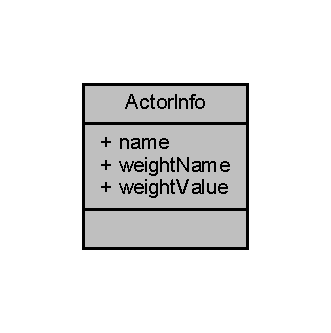
\includegraphics[width=159pt]{class_actor_info__coll__graph}
\end{center}
\end{figure}
\subsection*{Public 속성}
\begin{DoxyCompactItemize}
\item 
string \hyperlink{class_actor_info_a2e9e540cdc037f204d80622e47543410}{name}
\item 
List$<$ string $>$ \hyperlink{class_actor_info_a25bb8e0eafab630572ffddea088a1f80}{weight\+Name}
\item 
List$<$ int $>$ \hyperlink{class_actor_info_a1c5dd2d46e5ebc5a6483f2bcb55cb162}{weight\+Value}
\end{DoxyCompactItemize}


\subsection{상세한 설명}


Unit\+Actor\+Data.\+cs 파일의 24 번째 라인에서 정의되었습니다.



\subsection{멤버 데이타 문서화}
\index{Actor\+Info@{Actor\+Info}!name@{name}}
\index{name@{name}!Actor\+Info@{Actor\+Info}}
\subsubsection[{\texorpdfstring{name}{name}}]{\setlength{\rightskip}{0pt plus 5cm}string Actor\+Info.\+name}\hypertarget{class_actor_info_a2e9e540cdc037f204d80622e47543410}{}\label{class_actor_info_a2e9e540cdc037f204d80622e47543410}


Unit\+Actor\+Data.\+cs 파일의 26 번째 라인에서 정의되었습니다.

\index{Actor\+Info@{Actor\+Info}!weight\+Name@{weight\+Name}}
\index{weight\+Name@{weight\+Name}!Actor\+Info@{Actor\+Info}}
\subsubsection[{\texorpdfstring{weight\+Name}{weightName}}]{\setlength{\rightskip}{0pt plus 5cm}List$<$string$>$ Actor\+Info.\+weight\+Name}\hypertarget{class_actor_info_a25bb8e0eafab630572ffddea088a1f80}{}\label{class_actor_info_a25bb8e0eafab630572ffddea088a1f80}


Unit\+Actor\+Data.\+cs 파일의 27 번째 라인에서 정의되었습니다.

\index{Actor\+Info@{Actor\+Info}!weight\+Value@{weight\+Value}}
\index{weight\+Value@{weight\+Value}!Actor\+Info@{Actor\+Info}}
\subsubsection[{\texorpdfstring{weight\+Value}{weightValue}}]{\setlength{\rightskip}{0pt plus 5cm}List$<$int$>$ Actor\+Info.\+weight\+Value}\hypertarget{class_actor_info_a1c5dd2d46e5ebc5a6483f2bcb55cb162}{}\label{class_actor_info_a1c5dd2d46e5ebc5a6483f2bcb55cb162}


Unit\+Actor\+Data.\+cs 파일의 28 번째 라인에서 정의되었습니다.



이 클래스에 대한 문서화 페이지는 다음의 파일로부터 생성되었습니다.\+:\begin{DoxyCompactItemize}
\item 
D\+:/\+Git\+Hub/\+M\+C\+N\+Tactics/\+Assets/\+Scripts/\+Data/\hyperlink{_unit_actor_data_8cs}{Unit\+Actor\+Data.\+cs}\end{DoxyCompactItemize}

\hypertarget{class_f_z_1_1_actor_machine}{}\section{F\+Z.\+Actor\+Machine 클래스 참조}
\label{class_f_z_1_1_actor_machine}\index{F\+Z.\+Actor\+Machine@{F\+Z.\+Actor\+Machine}}


F\+Z.\+Actor\+Machine에 대한 상속 다이어그램 \+: 
% FIG 0


F\+Z.\+Actor\+Machine에 대한 협력 다이어그램\+:
% FIG 1
\subsection*{Public 멤버 함수}
\begin{DoxyCompactItemize}
\item 
void \hyperlink{class_f_z_1_1_actor_machine_abf6949bf5213c6b7eb9f7b2d0c677a23}{Add\+Actor} (\hyperlink{class_f_z_1_1_actor}{F\+Z.\+Actor} actor)
\item 
void \hyperlink{class_f_z_1_1_actor_machine_ac399a880001dbecdc39c1807f81e4eac}{Enqueue\+Actor} (System.\+Type actor\+Type)
\item 
\hyperlink{class_f_z_1_1_actor}{F\+Z.\+Actor} \hyperlink{class_f_z_1_1_actor_machine_a9f1efcf25b000d4634abcc97d361c629}{Get\+Active\+Actor} ()
\item 
void \hyperlink{class_f_z_1_1_actor_machine_a469fc3e9b02b02a2a8efb3e4c1e4101d}{Dequeue\+Actor} ()
\end{DoxyCompactItemize}
\subsection*{Private 속성}
\begin{DoxyCompactItemize}
\item 
Linked\+List$<$ \hyperlink{class_f_z_1_1_actor}{F\+Z.\+Actor} $>$ \hyperlink{class_f_z_1_1_actor_machine_a826fc2f6d597a9bca608d75bae961c0b}{\+\_\+actor\+Queue} = new Linked\+List$<$\hyperlink{class_f_z_1_1_actor}{F\+Z.\+Actor}$>$()
\item 
Dictionary$<$ string, \hyperlink{class_f_z_1_1_actor}{F\+Z.\+Actor} $>$ \hyperlink{class_f_z_1_1_actor_machine_a4c843d618b443f77c4ff40286f03f6b5}{\+\_\+actors} = new Dictionary$<$string, \hyperlink{class_f_z_1_1_actor}{F\+Z.\+Actor}$>$()
\end{DoxyCompactItemize}


\subsection{상세한 설명}


Actor.\+cs 파일의 160 번째 라인에서 정의되었습니다.



\subsection{멤버 함수 문서화}
\index{F\+Z\+::\+Actor\+Machine@{F\+Z\+::\+Actor\+Machine}!Add\+Actor@{Add\+Actor}}
\index{Add\+Actor@{Add\+Actor}!F\+Z\+::\+Actor\+Machine@{F\+Z\+::\+Actor\+Machine}}
\subsubsection[{\texorpdfstring{Add\+Actor(\+F\+Z.\+Actor actor)}{AddActor(FZ.Actor actor)}}]{\setlength{\rightskip}{0pt plus 5cm}void F\+Z.\+Actor\+Machine.\+Add\+Actor (
\begin{DoxyParamCaption}
\item[{{\bf F\+Z.\+Actor}}]{actor}
\end{DoxyParamCaption}
)}\hypertarget{class_f_z_1_1_actor_machine_abf6949bf5213c6b7eb9f7b2d0c677a23}{}\label{class_f_z_1_1_actor_machine_abf6949bf5213c6b7eb9f7b2d0c677a23}


\hyperlink{interface_f_z_1_1_i_actor_queue_a913b199f922223b26cf05efa96c14139}{F\+Z.\+I\+Actor\+Queue}를 구현.



Actor.\+cs 파일의 168 번째 라인에서 정의되었습니다.


\begin{DoxyCode}
169         \{
170             \textcolor{keywordflow}{if} (actor.CheckAbsoluteWeightKey())
171             \{
172                 \hyperlink{class_f_z_1_1_actor_machine_a4c843d618b443f77c4ff40286f03f6b5}{\_actors}.Add(actor.GetType().ToString(), actor);
173             \}
174         \}
\end{DoxyCode}


이 함수를 호출하는 함수들에 대한 그래프입니다.\+:
% FIG 2


\index{F\+Z\+::\+Actor\+Machine@{F\+Z\+::\+Actor\+Machine}!Dequeue\+Actor@{Dequeue\+Actor}}
\index{Dequeue\+Actor@{Dequeue\+Actor}!F\+Z\+::\+Actor\+Machine@{F\+Z\+::\+Actor\+Machine}}
\subsubsection[{\texorpdfstring{Dequeue\+Actor()}{DequeueActor()}}]{\setlength{\rightskip}{0pt plus 5cm}void F\+Z.\+Actor\+Machine.\+Dequeue\+Actor (
\begin{DoxyParamCaption}
{}
\end{DoxyParamCaption}
)}\hypertarget{class_f_z_1_1_actor_machine_a469fc3e9b02b02a2a8efb3e4c1e4101d}{}\label{class_f_z_1_1_actor_machine_a469fc3e9b02b02a2a8efb3e4c1e4101d}


\hyperlink{interface_f_z_1_1_i_actor_queue_a4299dfbeb2b3296677ccfc02fe0eaad7}{F\+Z.\+I\+Actor\+Queue}를 구현.



Actor.\+cs 파일의 199 번째 라인에서 정의되었습니다.


\begin{DoxyCode}
200         \{
201             \textcolor{keywordflow}{if} (\hyperlink{class_f_z_1_1_actor_machine_a826fc2f6d597a9bca608d75bae961c0b}{\_actorQueue}.Count > 0)
202             \{
203                 \hyperlink{class_f_z_1_1_actor_machine_a826fc2f6d597a9bca608d75bae961c0b}{\_actorQueue}.RemoveFirst();
204             \}
205         \}
\end{DoxyCode}


이 함수를 호출하는 함수들에 대한 그래프입니다.\+:
% FIG 3


\index{F\+Z\+::\+Actor\+Machine@{F\+Z\+::\+Actor\+Machine}!Enqueue\+Actor@{Enqueue\+Actor}}
\index{Enqueue\+Actor@{Enqueue\+Actor}!F\+Z\+::\+Actor\+Machine@{F\+Z\+::\+Actor\+Machine}}
\subsubsection[{\texorpdfstring{Enqueue\+Actor(\+System.\+Type actor\+Type)}{EnqueueActor(System.Type actorType)}}]{\setlength{\rightskip}{0pt plus 5cm}void F\+Z.\+Actor\+Machine.\+Enqueue\+Actor (
\begin{DoxyParamCaption}
\item[{System.\+Type}]{actor\+Type}
\end{DoxyParamCaption}
)}\hypertarget{class_f_z_1_1_actor_machine_ac399a880001dbecdc39c1807f81e4eac}{}\label{class_f_z_1_1_actor_machine_ac399a880001dbecdc39c1807f81e4eac}


\hyperlink{interface_f_z_1_1_i_actor_queue_ad0ffa88154fd9f44e0a8828b31a10c03}{F\+Z.\+I\+Actor\+Queue}를 구현.



Actor.\+cs 파일의 176 번째 라인에서 정의되었습니다.


\begin{DoxyCode}
177         \{
178             \textcolor{keywordflow}{if} (!actorType.IsSubclassOf(typeof(\hyperlink{namespace_f_z}{FZ}.\hyperlink{class_f_z_1_1_actor}{Actor})) ||
179                !\hyperlink{class_f_z_1_1_actor_machine_a4c843d618b443f77c4ff40286f03f6b5}{\_actors}.ContainsKey(actorType.ToString()))
180             \{
181                 \textcolor{keywordflow}{throw} \textcolor{keyword}{new} UnityException(\textcolor{stringliteral}{"Actor's type is not correct."});
182             \}
183 
184             \hyperlink{class_f_z_1_1_actor_machine_a826fc2f6d597a9bca608d75bae961c0b}{\_actorQueue}.AddLast(\hyperlink{class_f_z_1_1_actor_machine_a4c843d618b443f77c4ff40286f03f6b5}{\_actors}[actorType.ToString()]);
185         \}
\end{DoxyCode}


이 함수를 호출하는 함수들에 대한 그래프입니다.\+:
% FIG 4


\index{F\+Z\+::\+Actor\+Machine@{F\+Z\+::\+Actor\+Machine}!Get\+Active\+Actor@{Get\+Active\+Actor}}
\index{Get\+Active\+Actor@{Get\+Active\+Actor}!F\+Z\+::\+Actor\+Machine@{F\+Z\+::\+Actor\+Machine}}
\subsubsection[{\texorpdfstring{Get\+Active\+Actor()}{GetActiveActor()}}]{\setlength{\rightskip}{0pt plus 5cm}{\bf F\+Z.\+Actor} F\+Z.\+Actor\+Machine.\+Get\+Active\+Actor (
\begin{DoxyParamCaption}
{}
\end{DoxyParamCaption}
)}\hypertarget{class_f_z_1_1_actor_machine_a9f1efcf25b000d4634abcc97d361c629}{}\label{class_f_z_1_1_actor_machine_a9f1efcf25b000d4634abcc97d361c629}


Actor.\+cs 파일의 187 번째 라인에서 정의되었습니다.


\begin{DoxyCode}
188         \{
189             \textcolor{keywordflow}{if} (\hyperlink{class_f_z_1_1_actor_machine_a826fc2f6d597a9bca608d75bae961c0b}{\_actorQueue}.Count > 0)
190             \{
191                 var actor = \hyperlink{class_f_z_1_1_actor_machine_a826fc2f6d597a9bca608d75bae961c0b}{\_actorQueue}.First.Value;
192 
193                 \textcolor{keywordflow}{return} actor;
194             \}
195 
196             \textcolor{keywordflow}{return} null;
197         \}
\end{DoxyCode}


이 함수를 호출하는 함수들에 대한 그래프입니다.\+:
% FIG 5




\subsection{멤버 데이타 문서화}
\index{F\+Z\+::\+Actor\+Machine@{F\+Z\+::\+Actor\+Machine}!\+\_\+actor\+Queue@{\+\_\+actor\+Queue}}
\index{\+\_\+actor\+Queue@{\+\_\+actor\+Queue}!F\+Z\+::\+Actor\+Machine@{F\+Z\+::\+Actor\+Machine}}
\subsubsection[{\texorpdfstring{\+\_\+actor\+Queue}{_actorQueue}}]{\setlength{\rightskip}{0pt plus 5cm}Linked\+List$<${\bf F\+Z.\+Actor}$>$ F\+Z.\+Actor\+Machine.\+\_\+actor\+Queue = new Linked\+List$<${\bf F\+Z.\+Actor}$>$()\hspace{0.3cm}{\ttfamily [private]}}\hypertarget{class_f_z_1_1_actor_machine_a826fc2f6d597a9bca608d75bae961c0b}{}\label{class_f_z_1_1_actor_machine_a826fc2f6d597a9bca608d75bae961c0b}


Actor.\+cs 파일의 163 번째 라인에서 정의되었습니다.

\index{F\+Z\+::\+Actor\+Machine@{F\+Z\+::\+Actor\+Machine}!\+\_\+actors@{\+\_\+actors}}
\index{\+\_\+actors@{\+\_\+actors}!F\+Z\+::\+Actor\+Machine@{F\+Z\+::\+Actor\+Machine}}
\subsubsection[{\texorpdfstring{\+\_\+actors}{_actors}}]{\setlength{\rightskip}{0pt plus 5cm}Dictionary$<$string, {\bf F\+Z.\+Actor}$>$ F\+Z.\+Actor\+Machine.\+\_\+actors = new Dictionary$<$string, {\bf F\+Z.\+Actor}$>$()\hspace{0.3cm}{\ttfamily [private]}}\hypertarget{class_f_z_1_1_actor_machine_a4c843d618b443f77c4ff40286f03f6b5}{}\label{class_f_z_1_1_actor_machine_a4c843d618b443f77c4ff40286f03f6b5}


Actor.\+cs 파일의 166 번째 라인에서 정의되었습니다.



이 클래스에 대한 문서화 페이지는 다음의 파일로부터 생성되었습니다.\+:\begin{DoxyCompactItemize}
\item 
D\+:/\+Git\+Hub/\+M\+C\+N\+Tactics/\+Assets/\+Scripts/\+Core/\hyperlink{_actor_8cs}{Actor.\+cs}\end{DoxyCompactItemize}

\hypertarget{class_attack_actor}{}\section{Attack\+Actor 클래스 참조}
\label{class_attack_actor}\index{Attack\+Actor@{Attack\+Actor}}


Attack\+Actor에 대한 상속 다이어그램 \+: 
\nopagebreak
\begin{figure}[H]
\begin{center}
\leavevmode
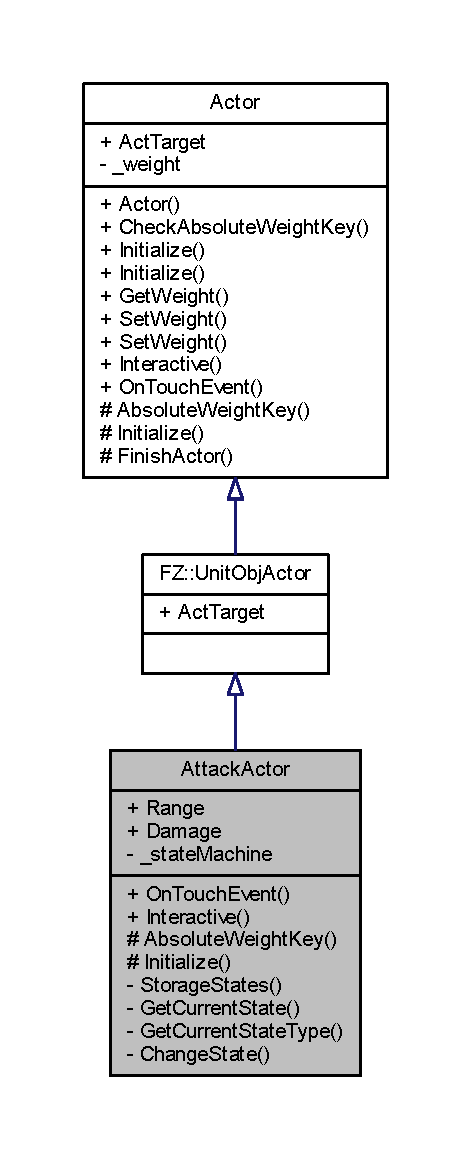
\includegraphics[width=226pt]{class_attack_actor__inherit__graph}
\end{center}
\end{figure}


Attack\+Actor에 대한 협력 다이어그램\+:
\nopagebreak
\begin{figure}[H]
\begin{center}
\leavevmode
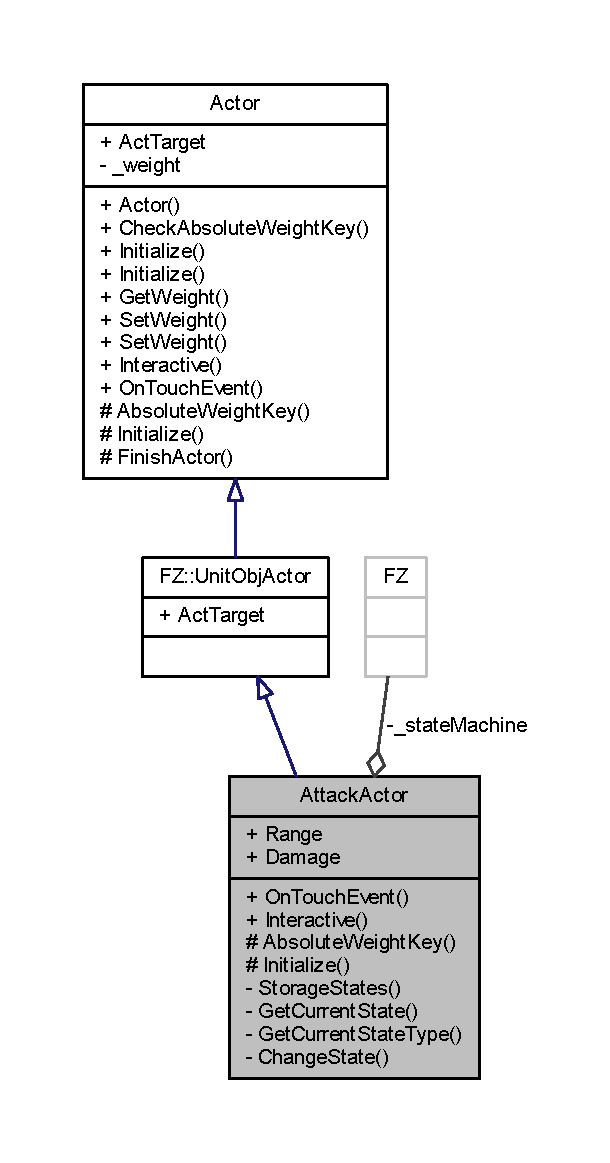
\includegraphics[width=303pt]{class_attack_actor__coll__graph}
\end{center}
\end{figure}
\subsection*{클래스}
\begin{DoxyCompactItemize}
\item 
class \hyperlink{class_attack_actor_1_1_attack_act_state}{Attack\+Act\+State}
\item 
class \hyperlink{class_attack_actor_1_1_attack_act_state___attack}{Attack\+Act\+State\+\_\+\+Attack}
\item 
class \hyperlink{class_attack_actor_1_1_attack_act_state___done}{Attack\+Act\+State\+\_\+\+Done}
\item 
class \hyperlink{class_attack_actor_1_1_attack_act_state___normal}{Attack\+Act\+State\+\_\+\+Normal}
\end{DoxyCompactItemize}
\subsection*{Public 멤버 함수}
\begin{DoxyCompactItemize}
\item 
override bool \hyperlink{class_attack_actor_a471c22dd21a49e9676a0e9d276cba709}{On\+Touch\+Event} (\hyperlink{_touch_manager_8cs_ae33e321a424fe84ba8b2fdb81ad40a68}{e\+Touch\+Event} touch)
\item 
override void \hyperlink{class_attack_actor_a766e164877bf499175dfb091967198a5}{Interactive} (\hyperlink{class_tactics_object}{Tactics\+Object} interact\+Target)
\item 
bool \hyperlink{class_m_c_n_1_1_actor_a493bb0a37cb9fc5b1aa8507ec69b04ac}{Check\+Absolute\+Weight\+Key} ()
\item 
void \hyperlink{class_m_c_n_1_1_actor_a27b307fecbbbf3aa53f8b5683de7ff36}{Initialize} (I\+Actor\+Queue act\+Target, List$<$ String\+Int\+Pair $>$ weights)
\item 
void \hyperlink{class_m_c_n_1_1_actor_ae5856541ad65c2c0ecc055414d20df0f}{Initialize} (I\+Actor\+Queue act\+Target, List$<$ string $>$ weight\+Name, List$<$ int $>$ weight\+Value)
\item 
int \hyperlink{class_m_c_n_1_1_actor_af264703ef93c3c77b5b7062aef828205}{Get\+Weight} (string key)
\item 
void \hyperlink{class_m_c_n_1_1_actor_a8d8020782aefa7fff625f5f8e09f7539}{Set\+Weight} (string key, int weight)
\item 
void \hyperlink{class_m_c_n_1_1_actor_a4337ef4d88c2086f18db4f2e6415eddd}{Set\+Weight} (Pair$<$ string, int $>$ info)
\end{DoxyCompactItemize}
\subsection*{Protected 멤버 함수}
\begin{DoxyCompactItemize}
\item 
override string\mbox{[}$\,$\mbox{]} \hyperlink{class_attack_actor_af120af42f4607f14a61928429f84eba5}{Absolute\+Weight\+Key} ()
\item 
override void \hyperlink{class_attack_actor_a6ecde7d8728f53eb75e5f5547deeec8e}{Initialize} ()
\item 
void \hyperlink{class_m_c_n_1_1_actor_ae86279ca7d290707cd010bc411f38966}{Finish\+Actor} ()
\end{DoxyCompactItemize}
\subsection*{속성}
\begin{DoxyCompactItemize}
\item 
int \hyperlink{class_attack_actor_aa331a3d1fbebd46a2458c64b209af927}{Range}\hspace{0.3cm}{\ttfamily  \mbox{[}get\mbox{]}}
\item 
int \hyperlink{class_attack_actor_aaa126531b12eeb6d03311d761697cc84}{Damage}\hspace{0.3cm}{\ttfamily  \mbox{[}get\mbox{]}}
\item 
I\+Actor\+Queue \hyperlink{class_m_c_n_1_1_actor_a1d809d2994dcccb6a8fcc665afa1ca6f}{Act\+Target}\hspace{0.3cm}{\ttfamily  \mbox{[}get, private set\mbox{]}}
\end{DoxyCompactItemize}
\subsection*{Private 멤버 함수}
\begin{DoxyCompactItemize}
\item 
void \hyperlink{class_attack_actor_a4c1408e09de62ad12b42bee3251556ba}{Storage\+States} ()
\item 
\hyperlink{class_attack_actor_1_1_attack_act_state}{Attack\+Act\+State} \hyperlink{class_attack_actor_ac231e370a4747dc36886f4158b289898}{Get\+Current\+State} ()
\item 
\hyperlink{_attack_actor_8cs_a10659ce944335df4ded984f6bc41f31b}{e\+Attack\+Act\+Type} \hyperlink{class_attack_actor_aab8bdc29ed7dae173129dbb09c9b8913}{Get\+Current\+State\+Type} ()
\item 
void \hyperlink{class_attack_actor_a97035efd9d67dd78cfa55cf321426567}{Change\+State} (\hyperlink{_attack_actor_8cs_a10659ce944335df4ded984f6bc41f31b}{e\+Attack\+Act\+Type} type)
\end{DoxyCompactItemize}
\subsection*{Private 속성}
\begin{DoxyCompactItemize}
\item 
\hyperlink{class_m_c_n_1_1_state_machine}{M\+C\+N.\+State\+Machine}$<$ \hyperlink{class_attack_actor_1_1_attack_act_state}{Attack\+Act\+State} $>$ \hyperlink{class_attack_actor_aefebe59645532f127c1504abb12ffac8}{\+\_\+state\+Machine} = new \hyperlink{class_m_c_n_1_1_state_machine}{M\+C\+N.\+State\+Machine}$<$\hyperlink{class_attack_actor_1_1_attack_act_state}{Attack\+Act\+State}$>$()
\end{DoxyCompactItemize}


\subsection{상세한 설명}


Attack\+Actor.\+cs 파일의 12 번째 라인에서 정의되었습니다.



\subsection{멤버 함수 문서화}
\index{Attack\+Actor@{Attack\+Actor}!Absolute\+Weight\+Key@{Absolute\+Weight\+Key}}
\index{Absolute\+Weight\+Key@{Absolute\+Weight\+Key}!Attack\+Actor@{Attack\+Actor}}
\subsubsection[{\texorpdfstring{Absolute\+Weight\+Key()}{AbsoluteWeightKey()}}]{\setlength{\rightskip}{0pt plus 5cm}override string \mbox{[}$\,$\mbox{]} Attack\+Actor.\+Absolute\+Weight\+Key (
\begin{DoxyParamCaption}
{}
\end{DoxyParamCaption}
)\hspace{0.3cm}{\ttfamily [protected]}, {\ttfamily [virtual]}}\hypertarget{class_attack_actor_af120af42f4607f14a61928429f84eba5}{}\label{class_attack_actor_af120af42f4607f14a61928429f84eba5}


\hyperlink{class_m_c_n_1_1_actor_a54340ddb597852fbb6e9f2a35663bbc5}{M\+C\+N.\+Actor}를 구현.



Attack\+Actor.\+cs 파일의 38 번째 라인에서 정의되었습니다.


\begin{DoxyCode}
39     \{
40         \textcolor{keywordflow}{return} \textcolor{keyword}{new} \textcolor{keywordtype}{string}[] \{ \textcolor{stringliteral}{"range"}, \textcolor{stringliteral}{"damage"} \};
41     \}
\end{DoxyCode}
\index{Attack\+Actor@{Attack\+Actor}!Change\+State@{Change\+State}}
\index{Change\+State@{Change\+State}!Attack\+Actor@{Attack\+Actor}}
\subsubsection[{\texorpdfstring{Change\+State(e\+Attack\+Act\+Type type)}{ChangeState(eAttackActType type)}}]{\setlength{\rightskip}{0pt plus 5cm}void Attack\+Actor.\+Change\+State (
\begin{DoxyParamCaption}
\item[{{\bf e\+Attack\+Act\+Type}}]{type}
\end{DoxyParamCaption}
)\hspace{0.3cm}{\ttfamily [private]}}\hypertarget{class_attack_actor_a97035efd9d67dd78cfa55cf321426567}{}\label{class_attack_actor_a97035efd9d67dd78cfa55cf321426567}


Attack\+Actor.\+cs 파일의 238 번째 라인에서 정의되었습니다.


\begin{DoxyCode}
239     \{
240         \textcolor{keywordflow}{if} (\hyperlink{class_attack_actor_aefebe59645532f127c1504abb12ffac8}{\_stateMachine} != null)
241         \{
242             \hyperlink{class_attack_actor_aefebe59645532f127c1504abb12ffac8}{\_stateMachine}.ChangeState(type.ToString());
243         \}
244     \}
\end{DoxyCode}


이 함수를 호출하는 함수들에 대한 그래프입니다.\+:
\nopagebreak
\begin{figure}[H]
\begin{center}
\leavevmode
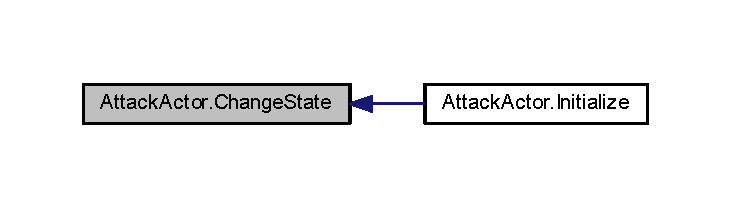
\includegraphics[width=350pt]{class_attack_actor_a97035efd9d67dd78cfa55cf321426567_icgraph}
\end{center}
\end{figure}


\index{Attack\+Actor@{Attack\+Actor}!Check\+Absolute\+Weight\+Key@{Check\+Absolute\+Weight\+Key}}
\index{Check\+Absolute\+Weight\+Key@{Check\+Absolute\+Weight\+Key}!Attack\+Actor@{Attack\+Actor}}
\subsubsection[{\texorpdfstring{Check\+Absolute\+Weight\+Key()}{CheckAbsoluteWeightKey()}}]{\setlength{\rightskip}{0pt plus 5cm}bool M\+C\+N.\+Actor.\+Check\+Absolute\+Weight\+Key (
\begin{DoxyParamCaption}
{}
\end{DoxyParamCaption}
)\hspace{0.3cm}{\ttfamily [inherited]}}\hypertarget{class_m_c_n_1_1_actor_a493bb0a37cb9fc5b1aa8507ec69b04ac}{}\label{class_m_c_n_1_1_actor_a493bb0a37cb9fc5b1aa8507ec69b04ac}


Actor.\+cs 파일의 29 번째 라인에서 정의되었습니다.


\begin{DoxyCode}
30         \{
31             \textcolor{keywordflow}{foreach} (var key \textcolor{keywordflow}{in} \hyperlink{class_m_c_n_1_1_actor_a54340ddb597852fbb6e9f2a35663bbc5}{AbsoluteWeightKey}())
32             \{
33                 \textcolor{keywordflow}{if} (\hyperlink{class_m_c_n_1_1_actor_abf0c60f05e2a904b0b225b4839a7296d}{\_weight} == null || !\hyperlink{class_m_c_n_1_1_actor_abf0c60f05e2a904b0b225b4839a7296d}{\_weight}.ContainsKey(key))
34                 \{
35                     \textcolor{keywordflow}{throw} \textcolor{keyword}{new} UnityException(\textcolor{keywordtype}{string}.Format(\textcolor{stringliteral}{"\{0\} is not available. because weight '\{1\}' key
       is not initialized."}, this.GetType().Name, key));
36                 \}
37             \}
38 
39             \textcolor{keywordflow}{return} \textcolor{keyword}{true};
40         \}
\end{DoxyCode}
\index{Attack\+Actor@{Attack\+Actor}!Finish\+Actor@{Finish\+Actor}}
\index{Finish\+Actor@{Finish\+Actor}!Attack\+Actor@{Attack\+Actor}}
\subsubsection[{\texorpdfstring{Finish\+Actor()}{FinishActor()}}]{\setlength{\rightskip}{0pt plus 5cm}void M\+C\+N.\+Actor.\+Finish\+Actor (
\begin{DoxyParamCaption}
{}
\end{DoxyParamCaption}
)\hspace{0.3cm}{\ttfamily [protected]}, {\ttfamily [inherited]}}\hypertarget{class_m_c_n_1_1_actor_ae86279ca7d290707cd010bc411f38966}{}\label{class_m_c_n_1_1_actor_ae86279ca7d290707cd010bc411f38966}


Actor.\+cs 파일의 87 번째 라인에서 정의되었습니다.


\begin{DoxyCode}
88         \{
89             \textcolor{keywordflow}{if} (\hyperlink{class_m_c_n_1_1_actor_a1d809d2994dcccb6a8fcc665afa1ca6f}{ActTarget} != null)
90             \{
91                 \hyperlink{class_m_c_n_1_1_actor_a1d809d2994dcccb6a8fcc665afa1ca6f}{ActTarget}.\hyperlink{interface_m_c_n_1_1_i_actor_queue_ad99049ac93213b4a4f0e2d9aa76f6029}{DequeueActor}();
92             \}
93         \}
\end{DoxyCode}
\index{Attack\+Actor@{Attack\+Actor}!Get\+Current\+State@{Get\+Current\+State}}
\index{Get\+Current\+State@{Get\+Current\+State}!Attack\+Actor@{Attack\+Actor}}
\subsubsection[{\texorpdfstring{Get\+Current\+State()}{GetCurrentState()}}]{\setlength{\rightskip}{0pt plus 5cm}{\bf Attack\+Act\+State} Attack\+Actor.\+Get\+Current\+State (
\begin{DoxyParamCaption}
{}
\end{DoxyParamCaption}
)\hspace{0.3cm}{\ttfamily [private]}}\hypertarget{class_attack_actor_ac231e370a4747dc36886f4158b289898}{}\label{class_attack_actor_ac231e370a4747dc36886f4158b289898}


Attack\+Actor.\+cs 파일의 215 번째 라인에서 정의되었습니다.


\begin{DoxyCode}
216     \{
217         var state = \hyperlink{class_attack_actor_aefebe59645532f127c1504abb12ffac8}{\_stateMachine}.GetCurrentState();
218         \textcolor{keywordflow}{if} (state != null && state is AttackActState)
219         \{
220             \textcolor{keywordflow}{return} state as AttackActState;
221         \}
222 
223         \textcolor{keywordflow}{throw} \textcolor{keyword}{new} UnityException(\textcolor{stringliteral}{"don't have attackAct state."});
224     \}
\end{DoxyCode}


이 함수 내부에서 호출하는 함수들에 대한 그래프입니다.\+:
\nopagebreak
\begin{figure}[H]
\begin{center}
\leavevmode
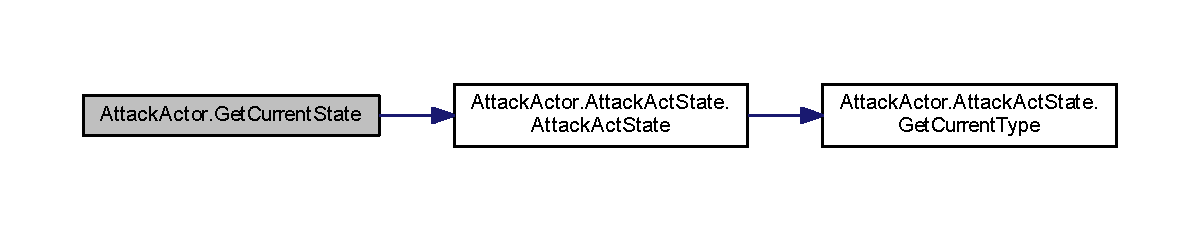
\includegraphics[width=350pt]{class_attack_actor_ac231e370a4747dc36886f4158b289898_cgraph}
\end{center}
\end{figure}




이 함수를 호출하는 함수들에 대한 그래프입니다.\+:
\nopagebreak
\begin{figure}[H]
\begin{center}
\leavevmode
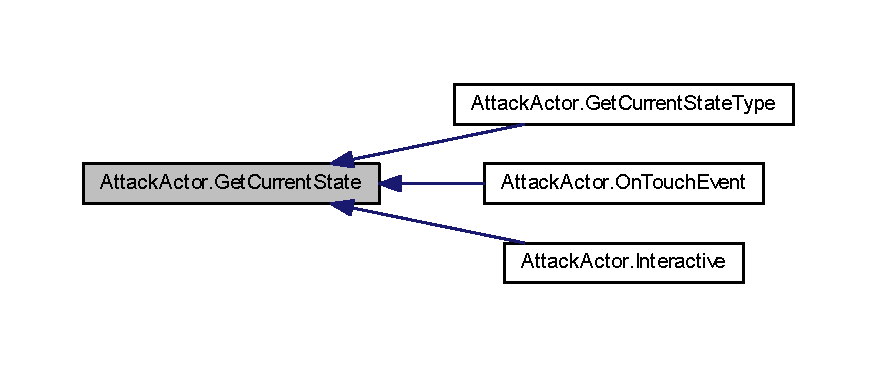
\includegraphics[width=350pt]{class_attack_actor_ac231e370a4747dc36886f4158b289898_icgraph}
\end{center}
\end{figure}


\index{Attack\+Actor@{Attack\+Actor}!Get\+Current\+State\+Type@{Get\+Current\+State\+Type}}
\index{Get\+Current\+State\+Type@{Get\+Current\+State\+Type}!Attack\+Actor@{Attack\+Actor}}
\subsubsection[{\texorpdfstring{Get\+Current\+State\+Type()}{GetCurrentStateType()}}]{\setlength{\rightskip}{0pt plus 5cm}{\bf e\+Attack\+Act\+Type} Attack\+Actor.\+Get\+Current\+State\+Type (
\begin{DoxyParamCaption}
{}
\end{DoxyParamCaption}
)\hspace{0.3cm}{\ttfamily [private]}}\hypertarget{class_attack_actor_aab8bdc29ed7dae173129dbb09c9b8913}{}\label{class_attack_actor_aab8bdc29ed7dae173129dbb09c9b8913}


Attack\+Actor.\+cs 파일의 226 번째 라인에서 정의되었습니다.


\begin{DoxyCode}
227     \{
228         var state = \hyperlink{class_attack_actor_ac231e370a4747dc36886f4158b289898}{GetCurrentState}();
229 
230         \textcolor{keywordflow}{if} (state != null)
231         \{
232             \textcolor{keywordflow}{return} state.GetCurrentType();
233         \}
234 
235         \textcolor{keywordflow}{throw} \textcolor{keyword}{new} UnityException(\textcolor{stringliteral}{"don't have attackAct state."});
236     \}
\end{DoxyCode}


이 함수 내부에서 호출하는 함수들에 대한 그래프입니다.\+:
\nopagebreak
\begin{figure}[H]
\begin{center}
\leavevmode
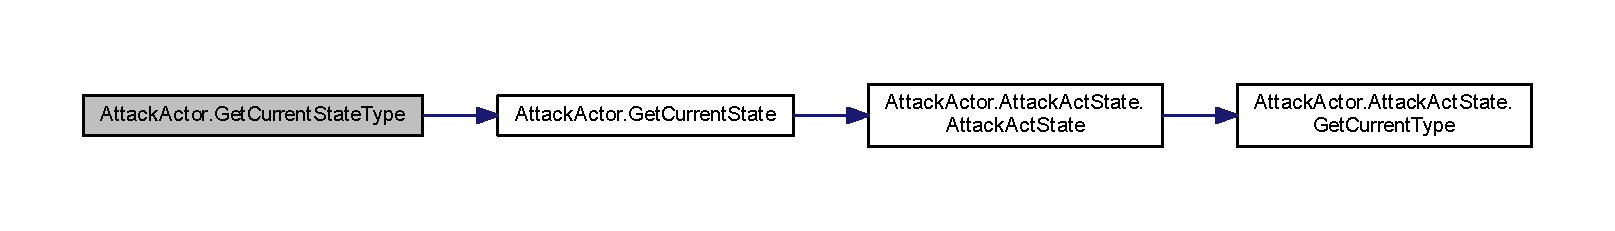
\includegraphics[width=350pt]{class_attack_actor_aab8bdc29ed7dae173129dbb09c9b8913_cgraph}
\end{center}
\end{figure}


\index{Attack\+Actor@{Attack\+Actor}!Get\+Weight@{Get\+Weight}}
\index{Get\+Weight@{Get\+Weight}!Attack\+Actor@{Attack\+Actor}}
\subsubsection[{\texorpdfstring{Get\+Weight(string key)}{GetWeight(string key)}}]{\setlength{\rightskip}{0pt plus 5cm}int M\+C\+N.\+Actor.\+Get\+Weight (
\begin{DoxyParamCaption}
\item[{string}]{key}
\end{DoxyParamCaption}
)\hspace{0.3cm}{\ttfamily [inherited]}}\hypertarget{class_m_c_n_1_1_actor_af264703ef93c3c77b5b7062aef828205}{}\label{class_m_c_n_1_1_actor_af264703ef93c3c77b5b7062aef828205}


Actor.\+cs 파일의 95 번째 라인에서 정의되었습니다.


\begin{DoxyCode}
96         \{
97             \textcolor{keywordflow}{if} (\hyperlink{class_m_c_n_1_1_actor_abf0c60f05e2a904b0b225b4839a7296d}{\_weight}.ContainsKey(key))
98             \{
99                 \textcolor{keywordflow}{return} \hyperlink{class_m_c_n_1_1_actor_abf0c60f05e2a904b0b225b4839a7296d}{\_weight}[key];
100             \}
101 
102             \textcolor{keywordflow}{return} 0;
103         \}
\end{DoxyCode}
\index{Attack\+Actor@{Attack\+Actor}!Initialize@{Initialize}}
\index{Initialize@{Initialize}!Attack\+Actor@{Attack\+Actor}}
\subsubsection[{\texorpdfstring{Initialize(\+I\+Actor\+Queue act\+Target, List$<$ String\+Int\+Pair $>$ weights)}{Initialize(IActorQueue actTarget, List< StringIntPair > weights)}}]{\setlength{\rightskip}{0pt plus 5cm}void M\+C\+N.\+Actor.\+Initialize (
\begin{DoxyParamCaption}
\item[{{\bf I\+Actor\+Queue}}]{act\+Target, }
\item[{List$<$ {\bf String\+Int\+Pair} $>$}]{weights}
\end{DoxyParamCaption}
)\hspace{0.3cm}{\ttfamily [inherited]}}\hypertarget{class_m_c_n_1_1_actor_a27b307fecbbbf3aa53f8b5683de7ff36}{}\label{class_m_c_n_1_1_actor_a27b307fecbbbf3aa53f8b5683de7ff36}


Actor.\+cs 파일의 42 번째 라인에서 정의되었습니다.


\begin{DoxyCode}
43         \{
44             \textcolor{keywordflow}{if} (actTarget == null)
45             \{
46                 \textcolor{keywordflow}{throw} \textcolor{keyword}{new} UnityException(\textcolor{stringliteral}{"Act Target is null."});
47             \}
48 
49             this.\hyperlink{class_m_c_n_1_1_actor_a1d809d2994dcccb6a8fcc665afa1ca6f}{ActTarget} = actTarget;
50 
51             \textcolor{keywordflow}{foreach} (var actorWeight \textcolor{keywordflow}{in} weights)
52             \{
53                 \hyperlink{class_m_c_n_1_1_actor_a8d8020782aefa7fff625f5f8e09f7539}{SetWeight}(actorWeight);
54             \}
55 
56             \hyperlink{class_m_c_n_1_1_actor_a37e76fad4625e138478764ae6c5ce959}{Initialize}();
57         \}
\end{DoxyCode}


이 함수를 호출하는 함수들에 대한 그래프입니다.\+:
\nopagebreak
\begin{figure}[H]
\begin{center}
\leavevmode
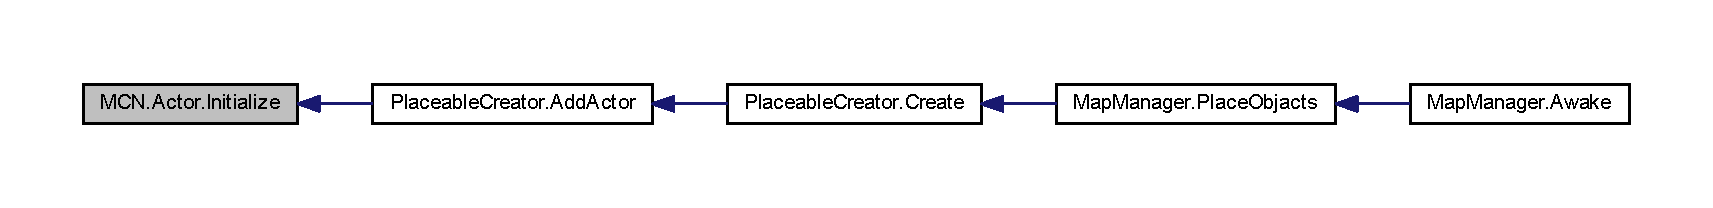
\includegraphics[width=350pt]{class_m_c_n_1_1_actor_a27b307fecbbbf3aa53f8b5683de7ff36_icgraph}
\end{center}
\end{figure}


\index{Attack\+Actor@{Attack\+Actor}!Initialize@{Initialize}}
\index{Initialize@{Initialize}!Attack\+Actor@{Attack\+Actor}}
\subsubsection[{\texorpdfstring{Initialize(\+I\+Actor\+Queue act\+Target, List$<$ string $>$ weight\+Name, List$<$ int $>$ weight\+Value)}{Initialize(IActorQueue actTarget, List< string > weightName, List< int > weightValue)}}]{\setlength{\rightskip}{0pt plus 5cm}void M\+C\+N.\+Actor.\+Initialize (
\begin{DoxyParamCaption}
\item[{{\bf I\+Actor\+Queue}}]{act\+Target, }
\item[{List$<$ string $>$}]{weight\+Name, }
\item[{List$<$ int $>$}]{weight\+Value}
\end{DoxyParamCaption}
)\hspace{0.3cm}{\ttfamily [inherited]}}\hypertarget{class_m_c_n_1_1_actor_ae5856541ad65c2c0ecc055414d20df0f}{}\label{class_m_c_n_1_1_actor_ae5856541ad65c2c0ecc055414d20df0f}


Actor.\+cs 파일의 59 번째 라인에서 정의되었습니다.


\begin{DoxyCode}
60         \{
61             \textcolor{keywordflow}{if} (actTarget == null)
62             \{
63                 \textcolor{keywordflow}{throw} \textcolor{keyword}{new} UnityException(\textcolor{stringliteral}{"Act Target is null."});
64             \}
65 
66             this.\hyperlink{class_m_c_n_1_1_actor_a1d809d2994dcccb6a8fcc665afa1ca6f}{ActTarget} = actTarget;
67 
68             \textcolor{keywordflow}{for} (\textcolor{keywordtype}{int} i = 0; i < weightName.Count; ++i)
69             \{
70                 var pair = \textcolor{keyword}{new} StringIntPair();
71 
72                 pair.key = weightName[i];
73 
74                 \textcolor{keywordflow}{if} (weightValue.Count > i)
75                 \{
76                     pair.value = weightValue[i];
77                 \}
78 
79                 \hyperlink{class_m_c_n_1_1_actor_a8d8020782aefa7fff625f5f8e09f7539}{SetWeight}(pair);
80             \}
81 
82             \hyperlink{class_m_c_n_1_1_actor_a37e76fad4625e138478764ae6c5ce959}{Initialize}();
83         \}
\end{DoxyCode}
\index{Attack\+Actor@{Attack\+Actor}!Initialize@{Initialize}}
\index{Initialize@{Initialize}!Attack\+Actor@{Attack\+Actor}}
\subsubsection[{\texorpdfstring{Initialize()}{Initialize()}}]{\setlength{\rightskip}{0pt plus 5cm}override void Attack\+Actor.\+Initialize (
\begin{DoxyParamCaption}
{}
\end{DoxyParamCaption}
)\hspace{0.3cm}{\ttfamily [protected]}, {\ttfamily [virtual]}}\hypertarget{class_attack_actor_a6ecde7d8728f53eb75e5f5547deeec8e}{}\label{class_attack_actor_a6ecde7d8728f53eb75e5f5547deeec8e}


\hyperlink{class_m_c_n_1_1_actor_a37e76fad4625e138478764ae6c5ce959}{M\+C\+N.\+Actor}(으)로부터 재구현되었습니다.



Attack\+Actor.\+cs 파일의 199 번째 라인에서 정의되었습니다.


\begin{DoxyCode}
200     \{
201         base.Initialize();
202 
203         \hyperlink{class_attack_actor_a4c1408e09de62ad12b42bee3251556ba}{StorageStates}();
204 
205         \hyperlink{class_attack_actor_a97035efd9d67dd78cfa55cf321426567}{ChangeState}(\hyperlink{_attack_actor_8cs_a10659ce944335df4ded984f6bc41f31b}{eAttackActType}.NORMAL);
206     \}
\end{DoxyCode}


이 함수 내부에서 호출하는 함수들에 대한 그래프입니다.\+:
\nopagebreak
\begin{figure}[H]
\begin{center}
\leavevmode
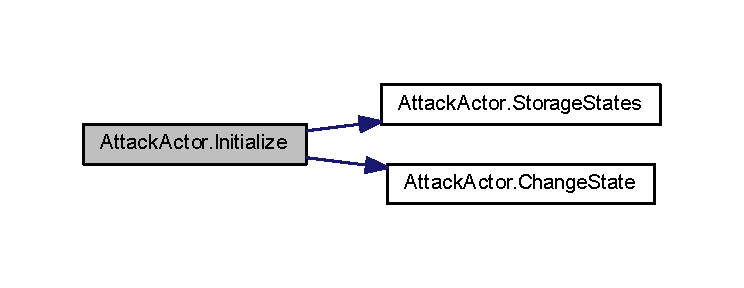
\includegraphics[width=350pt]{class_attack_actor_a6ecde7d8728f53eb75e5f5547deeec8e_cgraph}
\end{center}
\end{figure}


\index{Attack\+Actor@{Attack\+Actor}!Interactive@{Interactive}}
\index{Interactive@{Interactive}!Attack\+Actor@{Attack\+Actor}}
\subsubsection[{\texorpdfstring{Interactive(\+Tactics\+Object interact\+Target)}{Interactive(TacticsObject interactTarget)}}]{\setlength{\rightskip}{0pt plus 5cm}override void Attack\+Actor.\+Interactive (
\begin{DoxyParamCaption}
\item[{{\bf Tactics\+Object}}]{interact\+Target}
\end{DoxyParamCaption}
)\hspace{0.3cm}{\ttfamily [virtual]}}\hypertarget{class_attack_actor_a766e164877bf499175dfb091967198a5}{}\label{class_attack_actor_a766e164877bf499175dfb091967198a5}


\hyperlink{class_m_c_n_1_1_actor_a8ca8f46410f6ee9557e529e22fd6f6d1}{M\+C\+N.\+Actor}(으)로부터 재구현되었습니다.



Attack\+Actor.\+cs 파일의 260 번째 라인에서 정의되었습니다.


\begin{DoxyCode}
261     \{
262         base.Interactive(interactTarget);
263 
264         var tile = interactTarget as \hyperlink{class_tile}{Tile};
265 
266         \textcolor{keywordflow}{if} (tile != null)
267         \{
268             var state = \hyperlink{class_attack_actor_ac231e370a4747dc36886f4158b289898}{GetCurrentState}();
269 
270             \textcolor{keywordflow}{if} (state != null)
271             \{
272                 state.Interactive(tile);
273 
274                 \textcolor{keywordflow}{return};
275             \}
276         \}
277 
278         \textcolor{keywordflow}{throw} \textcolor{keyword}{new} UnityException(\textcolor{stringliteral}{"don't have attackAct state."});
279     \}
\end{DoxyCode}


이 함수 내부에서 호출하는 함수들에 대한 그래프입니다.\+:
\nopagebreak
\begin{figure}[H]
\begin{center}
\leavevmode
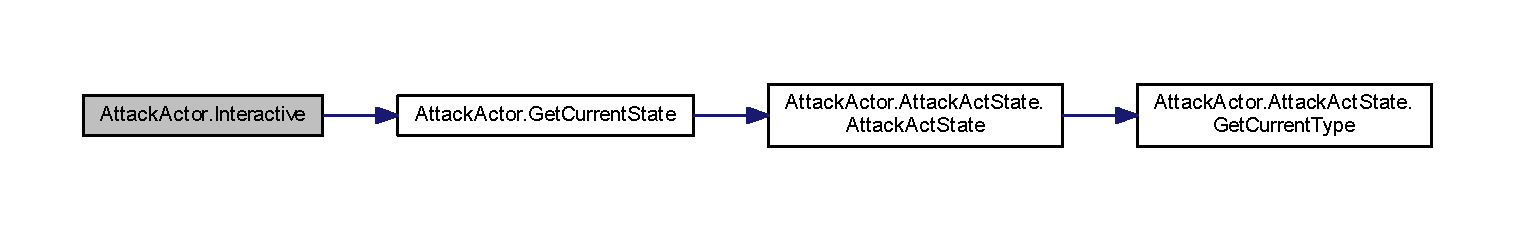
\includegraphics[width=350pt]{class_attack_actor_a766e164877bf499175dfb091967198a5_cgraph}
\end{center}
\end{figure}


\index{Attack\+Actor@{Attack\+Actor}!On\+Touch\+Event@{On\+Touch\+Event}}
\index{On\+Touch\+Event@{On\+Touch\+Event}!Attack\+Actor@{Attack\+Actor}}
\subsubsection[{\texorpdfstring{On\+Touch\+Event(e\+Touch\+Event touch)}{OnTouchEvent(eTouchEvent touch)}}]{\setlength{\rightskip}{0pt plus 5cm}override bool Attack\+Actor.\+On\+Touch\+Event (
\begin{DoxyParamCaption}
\item[{{\bf e\+Touch\+Event}}]{touch}
\end{DoxyParamCaption}
)\hspace{0.3cm}{\ttfamily [virtual]}}\hypertarget{class_attack_actor_a471c22dd21a49e9676a0e9d276cba709}{}\label{class_attack_actor_a471c22dd21a49e9676a0e9d276cba709}


\hyperlink{class_m_c_n_1_1_actor_a4891cf321e2a9ee25fd618c19b785331}{M\+C\+N.\+Actor}(으)로부터 재구현되었습니다.



Attack\+Actor.\+cs 파일의 246 번째 라인에서 정의되었습니다.


\begin{DoxyCode}
247     \{
248         base.OnTouchEvent(touch);
249 
250         var state = \hyperlink{class_attack_actor_ac231e370a4747dc36886f4158b289898}{GetCurrentState}();
251 
252         \textcolor{keywordflow}{if} (state != null)
253         \{
254             \textcolor{keywordflow}{return} state.OnTouchEvent();
255         \}
256 
257         \textcolor{keywordflow}{throw} \textcolor{keyword}{new} UnityException(\textcolor{stringliteral}{"don't have attackAct state."});
258     \}
\end{DoxyCode}


이 함수 내부에서 호출하는 함수들에 대한 그래프입니다.\+:
\nopagebreak
\begin{figure}[H]
\begin{center}
\leavevmode
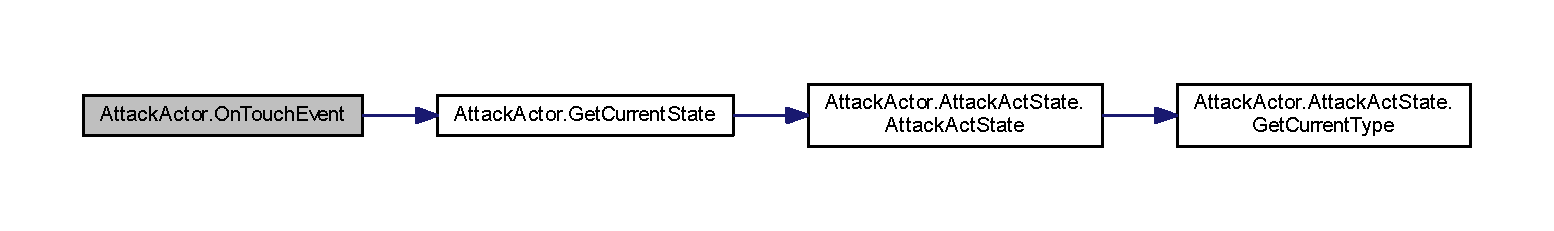
\includegraphics[width=350pt]{class_attack_actor_a471c22dd21a49e9676a0e9d276cba709_cgraph}
\end{center}
\end{figure}


\index{Attack\+Actor@{Attack\+Actor}!Set\+Weight@{Set\+Weight}}
\index{Set\+Weight@{Set\+Weight}!Attack\+Actor@{Attack\+Actor}}
\subsubsection[{\texorpdfstring{Set\+Weight(string key, int weight)}{SetWeight(string key, int weight)}}]{\setlength{\rightskip}{0pt plus 5cm}void M\+C\+N.\+Actor.\+Set\+Weight (
\begin{DoxyParamCaption}
\item[{string}]{key, }
\item[{int}]{weight}
\end{DoxyParamCaption}
)\hspace{0.3cm}{\ttfamily [inherited]}}\hypertarget{class_m_c_n_1_1_actor_a8d8020782aefa7fff625f5f8e09f7539}{}\label{class_m_c_n_1_1_actor_a8d8020782aefa7fff625f5f8e09f7539}


Actor.\+cs 파일의 105 번째 라인에서 정의되었습니다.


\begin{DoxyCode}
106         \{
107             \hyperlink{class_m_c_n_1_1_actor_abf0c60f05e2a904b0b225b4839a7296d}{\_weight}[key] = weight;
108         \}
\end{DoxyCode}
\index{Attack\+Actor@{Attack\+Actor}!Set\+Weight@{Set\+Weight}}
\index{Set\+Weight@{Set\+Weight}!Attack\+Actor@{Attack\+Actor}}
\subsubsection[{\texorpdfstring{Set\+Weight(\+Pair$<$ string, int $>$ info)}{SetWeight(Pair< string, int > info)}}]{\setlength{\rightskip}{0pt plus 5cm}void M\+C\+N.\+Actor.\+Set\+Weight (
\begin{DoxyParamCaption}
\item[{{\bf Pair}$<$ string, int $>$}]{info}
\end{DoxyParamCaption}
)\hspace{0.3cm}{\ttfamily [inherited]}}\hypertarget{class_m_c_n_1_1_actor_a4337ef4d88c2086f18db4f2e6415eddd}{}\label{class_m_c_n_1_1_actor_a4337ef4d88c2086f18db4f2e6415eddd}


Actor.\+cs 파일의 110 번째 라인에서 정의되었습니다.


\begin{DoxyCode}
111         \{
112             \textcolor{keywordflow}{if} (info != null)
113             \{
114                 \textcolor{keywordflow}{if} (\hyperlink{class_m_c_n_1_1_actor_abf0c60f05e2a904b0b225b4839a7296d}{\_weight} == null)
115                 \{
116                     \hyperlink{class_m_c_n_1_1_actor_abf0c60f05e2a904b0b225b4839a7296d}{\_weight} = \textcolor{keyword}{new} Dictionary<string, int>();
117                 \}
118 
119                 \hyperlink{class_m_c_n_1_1_actor_abf0c60f05e2a904b0b225b4839a7296d}{\_weight}[info.\hyperlink{class_m_c_n_1_1_pair_a62c546d3829b8819a65f8c9d64200338}{key}] = info.\hyperlink{class_m_c_n_1_1_pair_a1980bbf37b60fcbfea22382f71250e84}{value};
120             \}
121         \}
\end{DoxyCode}
\index{Attack\+Actor@{Attack\+Actor}!Storage\+States@{Storage\+States}}
\index{Storage\+States@{Storage\+States}!Attack\+Actor@{Attack\+Actor}}
\subsubsection[{\texorpdfstring{Storage\+States()}{StorageStates()}}]{\setlength{\rightskip}{0pt plus 5cm}void Attack\+Actor.\+Storage\+States (
\begin{DoxyParamCaption}
{}
\end{DoxyParamCaption}
)\hspace{0.3cm}{\ttfamily [private]}}\hypertarget{class_attack_actor_a4c1408e09de62ad12b42bee3251556ba}{}\label{class_attack_actor_a4c1408e09de62ad12b42bee3251556ba}


Attack\+Actor.\+cs 파일의 208 번째 라인에서 정의되었습니다.


\begin{DoxyCode}
209     \{
210         \textcolor{keyword}{new} AttackActState\_Normal(\textcolor{keyword}{this});
211         \textcolor{keyword}{new} AttackActState\_Attack(\textcolor{keyword}{this});
212         \textcolor{keyword}{new} AttackActState\_Done(\textcolor{keyword}{this});
213     \}
\end{DoxyCode}


이 함수를 호출하는 함수들에 대한 그래프입니다.\+:
\nopagebreak
\begin{figure}[H]
\begin{center}
\leavevmode
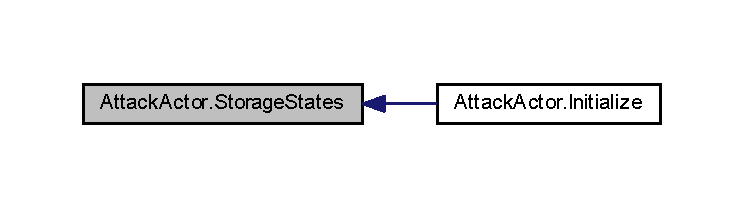
\includegraphics[width=350pt]{class_attack_actor_a4c1408e09de62ad12b42bee3251556ba_icgraph}
\end{center}
\end{figure}




\subsection{멤버 데이타 문서화}
\index{Attack\+Actor@{Attack\+Actor}!\+\_\+state\+Machine@{\+\_\+state\+Machine}}
\index{\+\_\+state\+Machine@{\+\_\+state\+Machine}!Attack\+Actor@{Attack\+Actor}}
\subsubsection[{\texorpdfstring{\+\_\+state\+Machine}{_stateMachine}}]{\setlength{\rightskip}{0pt plus 5cm}{\bf M\+C\+N.\+State\+Machine}$<${\bf Attack\+Act\+State}$>$ Attack\+Actor.\+\_\+state\+Machine = new {\bf M\+C\+N.\+State\+Machine}$<${\bf Attack\+Act\+State}$>$()\hspace{0.3cm}{\ttfamily [private]}}\hypertarget{class_attack_actor_aefebe59645532f127c1504abb12ffac8}{}\label{class_attack_actor_aefebe59645532f127c1504abb12ffac8}


Attack\+Actor.\+cs 파일의 45 번째 라인에서 정의되었습니다.



\subsection{속성 문서화}
\index{Attack\+Actor@{Attack\+Actor}!Act\+Target@{Act\+Target}}
\index{Act\+Target@{Act\+Target}!Attack\+Actor@{Attack\+Actor}}
\subsubsection[{\texorpdfstring{Act\+Target}{ActTarget}}]{\setlength{\rightskip}{0pt plus 5cm}I\+Actor\+Queue M\+C\+N.\+Actor.\+Act\+Target\hspace{0.3cm}{\ttfamily [get]}, {\ttfamily [private set]}, {\ttfamily [protected]}, {\ttfamily [inherited]}}\hypertarget{class_m_c_n_1_1_actor_a1d809d2994dcccb6a8fcc665afa1ca6f}{}\label{class_m_c_n_1_1_actor_a1d809d2994dcccb6a8fcc665afa1ca6f}


Actor.\+cs 파일의 23 번째 라인에서 정의되었습니다.

\index{Attack\+Actor@{Attack\+Actor}!Damage@{Damage}}
\index{Damage@{Damage}!Attack\+Actor@{Attack\+Actor}}
\subsubsection[{\texorpdfstring{Damage}{Damage}}]{\setlength{\rightskip}{0pt plus 5cm}int Attack\+Actor.\+Damage\hspace{0.3cm}{\ttfamily [get]}}\hypertarget{class_attack_actor_aaa126531b12eeb6d03311d761697cc84}{}\label{class_attack_actor_aaa126531b12eeb6d03311d761697cc84}


Attack\+Actor.\+cs 파일의 24 번째 라인에서 정의되었습니다.

\index{Attack\+Actor@{Attack\+Actor}!Range@{Range}}
\index{Range@{Range}!Attack\+Actor@{Attack\+Actor}}
\subsubsection[{\texorpdfstring{Range}{Range}}]{\setlength{\rightskip}{0pt plus 5cm}int Attack\+Actor.\+Range\hspace{0.3cm}{\ttfamily [get]}}\hypertarget{class_attack_actor_aa331a3d1fbebd46a2458c64b209af927}{}\label{class_attack_actor_aa331a3d1fbebd46a2458c64b209af927}


Attack\+Actor.\+cs 파일의 16 번째 라인에서 정의되었습니다.



이 클래스에 대한 문서화 페이지는 다음의 파일로부터 생성되었습니다.\+:\begin{DoxyCompactItemize}
\item 
D\+:/\+Git\+Hub/\+M\+C\+N\+Tactics/\+Assets/\+Scripts/\+Objects/\+Actor/\hyperlink{_attack_actor_8cs}{Attack\+Actor.\+cs}\end{DoxyCompactItemize}

\hypertarget{class_attack_actor_1_1_attack_act_state}{}\section{Attack\+Actor.\+Attack\+Act\+State 클래스 참조}
\label{class_attack_actor_1_1_attack_act_state}\index{Attack\+Actor.\+Attack\+Act\+State@{Attack\+Actor.\+Attack\+Act\+State}}


Attack\+Actor.\+Attack\+Act\+State에 대한 상속 다이어그램 \+: 
\nopagebreak
\begin{figure}[H]
\begin{center}
\leavevmode
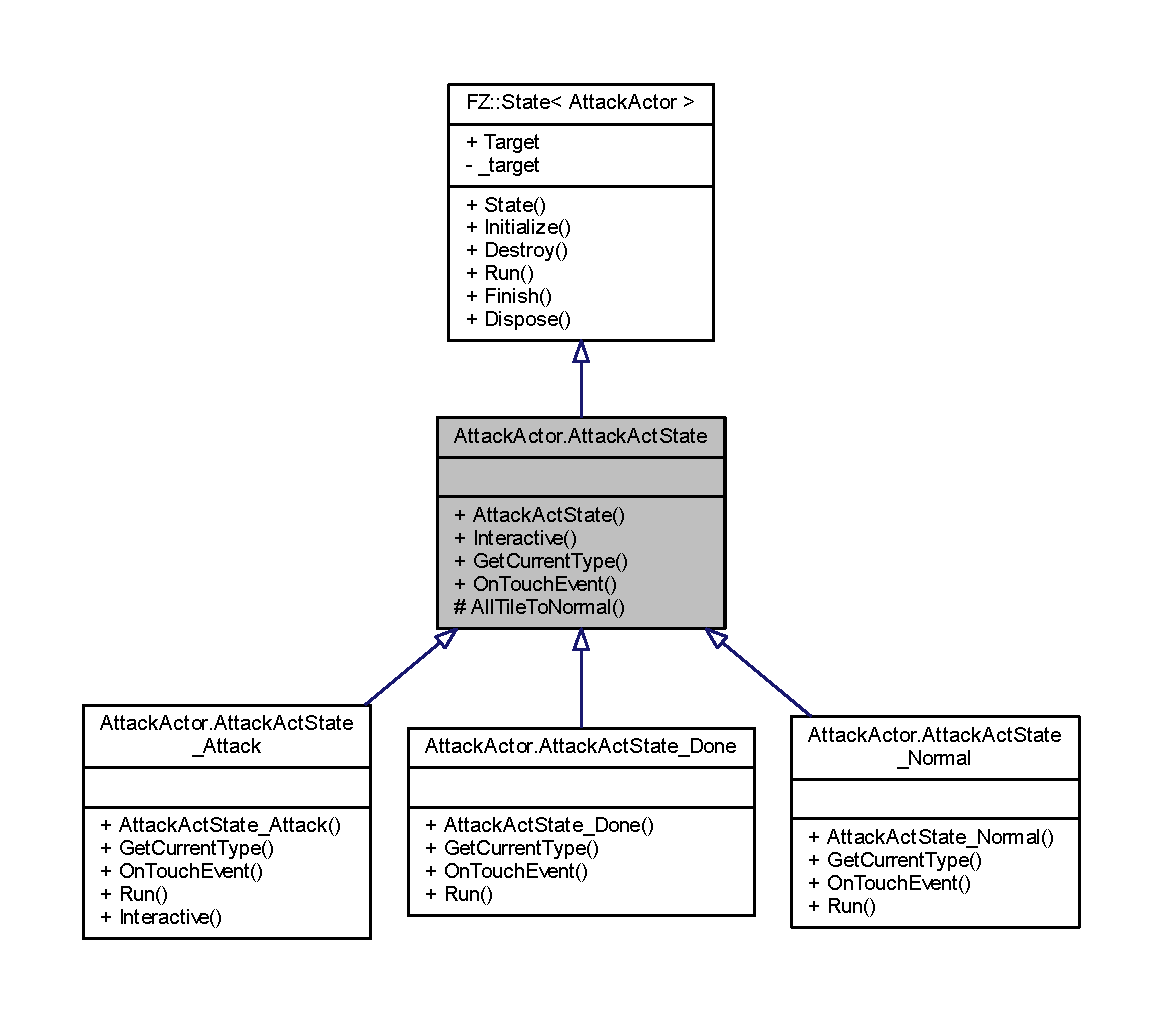
\includegraphics[width=350pt]{class_attack_actor_1_1_attack_act_state__inherit__graph}
\end{center}
\end{figure}


Attack\+Actor.\+Attack\+Act\+State에 대한 협력 다이어그램\+:
\nopagebreak
\begin{figure}[H]
\begin{center}
\leavevmode
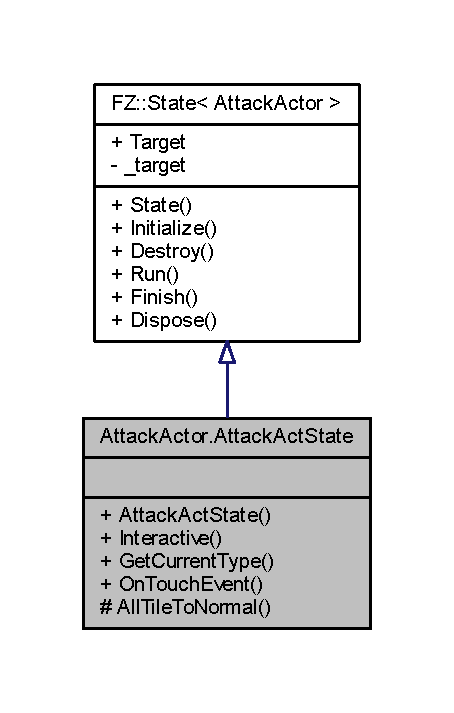
\includegraphics[width=218pt]{class_attack_actor_1_1_attack_act_state__coll__graph}
\end{center}
\end{figure}
\subsection*{Public 멤버 함수}
\begin{DoxyCompactItemize}
\item 
\hyperlink{class_attack_actor_1_1_attack_act_state_ab084b28b7bfaec2033a5102a48303af5}{Attack\+Act\+State} (\hyperlink{class_attack_actor}{Attack\+Actor} target)
\item 
virtual void \hyperlink{class_attack_actor_1_1_attack_act_state_a2ae9dd2f7ec8db76d25d7ad7ed58b89d}{Interactive} (\hyperlink{class_tile}{Tile} active\+Tile)
\item 
abstract \hyperlink{_attack_actor_8cs_a10659ce944335df4ded984f6bc41f31b}{e\+Attack\+Act\+Type} \hyperlink{class_attack_actor_1_1_attack_act_state_a8657ce92996ace441bb68b9e3002aa56}{Get\+Current\+Type} ()
\item 
abstract bool \hyperlink{class_attack_actor_1_1_attack_act_state_aa5e1794a3ede54c3b71a1463bf5b79a4}{On\+Touch\+Event} ()
\item 
virtual void \hyperlink{class_m_c_n_1_1_state_a8eabaffe047e6dccd5c5d8aed7bf218a}{Initialize} ()
\item 
virtual void \hyperlink{class_m_c_n_1_1_state_a32af22a6a0a979d3b3a80225426aa839}{Destroy} ()
\item 
abstract void \hyperlink{class_m_c_n_1_1_state_a8adfea67c55997e5c0eefbae1e429f4d}{Run} ()
\item 
virtual void \hyperlink{class_m_c_n_1_1_state_a6de4f94b23916fcd05f589759da9ac3f}{Finish} ()
\item 
void \hyperlink{class_m_c_n_1_1_state_a6c53b2eda47e718ff469fd76a95cf02a}{Dispose} ()
\end{DoxyCompactItemize}
\subsection*{Protected 멤버 함수}
\begin{DoxyCompactItemize}
\item 
void \hyperlink{class_attack_actor_1_1_attack_act_state_a993762ec959af926e416f03fa7b71203}{All\+Tile\+To\+Normal} ()
\end{DoxyCompactItemize}
\subsection*{속성}
\begin{DoxyCompactItemize}
\item 
T \hyperlink{class_m_c_n_1_1_state_a93ba2fd920292031bd6e65b1dc505cb3}{Target}\hspace{0.3cm}{\ttfamily  \mbox{[}get\mbox{]}}
\end{DoxyCompactItemize}


\subsection{상세한 설명}


Attack\+Actor.\+cs 파일의 47 번째 라인에서 정의되었습니다.



\subsection{생성자 \& 소멸자 문서화}
\index{Attack\+Actor\+::\+Attack\+Act\+State@{Attack\+Actor\+::\+Attack\+Act\+State}!Attack\+Act\+State@{Attack\+Act\+State}}
\index{Attack\+Act\+State@{Attack\+Act\+State}!Attack\+Actor\+::\+Attack\+Act\+State@{Attack\+Actor\+::\+Attack\+Act\+State}}
\subsubsection[{\texorpdfstring{Attack\+Act\+State(\+Attack\+Actor target)}{AttackActState(AttackActor target)}}]{\setlength{\rightskip}{0pt plus 5cm}Attack\+Actor.\+Attack\+Act\+State.\+Attack\+Act\+State (
\begin{DoxyParamCaption}
\item[{{\bf Attack\+Actor}}]{target}
\end{DoxyParamCaption}
)}\hypertarget{class_attack_actor_1_1_attack_act_state_ab084b28b7bfaec2033a5102a48303af5}{}\label{class_attack_actor_1_1_attack_act_state_ab084b28b7bfaec2033a5102a48303af5}


Attack\+Actor.\+cs 파일의 49 번째 라인에서 정의되었습니다.


\begin{DoxyCode}
49                                                   : base(target)
50         \{
51             \textcolor{keywordflow}{if} (\hyperlink{class_m_c_n_1_1_state_a93ba2fd920292031bd6e65b1dc505cb3}{Target} != null && \hyperlink{class_m_c_n_1_1_state_a93ba2fd920292031bd6e65b1dc505cb3}{Target}.\_stateMachine != null)
52             \{
53                 \hyperlink{class_m_c_n_1_1_state_a93ba2fd920292031bd6e65b1dc505cb3}{Target}.\_stateMachine.StorageState(\hyperlink{class_attack_actor_1_1_attack_act_state_a8657ce92996ace441bb68b9e3002aa56}{GetCurrentType}().ToString(), \textcolor{keyword}{this});
54             \}
55         \}
\end{DoxyCode}


이 함수 내부에서 호출하는 함수들에 대한 그래프입니다.\+:
\nopagebreak
\begin{figure}[H]
\begin{center}
\leavevmode
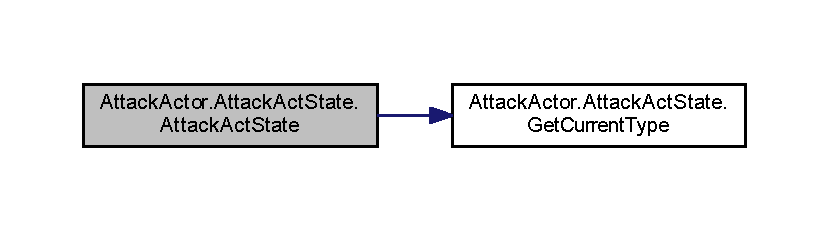
\includegraphics[width=350pt]{class_attack_actor_1_1_attack_act_state_ab084b28b7bfaec2033a5102a48303af5_cgraph}
\end{center}
\end{figure}




이 함수를 호출하는 함수들에 대한 그래프입니다.\+:
\nopagebreak
\begin{figure}[H]
\begin{center}
\leavevmode
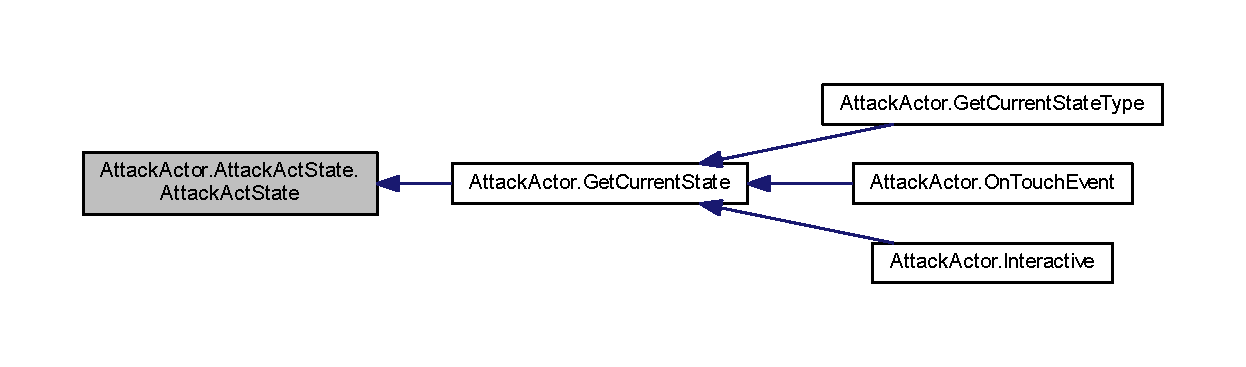
\includegraphics[width=350pt]{class_attack_actor_1_1_attack_act_state_ab084b28b7bfaec2033a5102a48303af5_icgraph}
\end{center}
\end{figure}




\subsection{멤버 함수 문서화}
\index{Attack\+Actor\+::\+Attack\+Act\+State@{Attack\+Actor\+::\+Attack\+Act\+State}!All\+Tile\+To\+Normal@{All\+Tile\+To\+Normal}}
\index{All\+Tile\+To\+Normal@{All\+Tile\+To\+Normal}!Attack\+Actor\+::\+Attack\+Act\+State@{Attack\+Actor\+::\+Attack\+Act\+State}}
\subsubsection[{\texorpdfstring{All\+Tile\+To\+Normal()}{AllTileToNormal()}}]{\setlength{\rightskip}{0pt plus 5cm}void Attack\+Actor.\+Attack\+Act\+State.\+All\+Tile\+To\+Normal (
\begin{DoxyParamCaption}
{}
\end{DoxyParamCaption}
)\hspace{0.3cm}{\ttfamily [protected]}}\hypertarget{class_attack_actor_1_1_attack_act_state_a993762ec959af926e416f03fa7b71203}{}\label{class_attack_actor_1_1_attack_act_state_a993762ec959af926e416f03fa7b71203}


Attack\+Actor.\+cs 파일의 63 번째 라인에서 정의되었습니다.


\begin{DoxyCode}
64         \{
65             \textcolor{keywordflow}{if} (\hyperlink{class_m_c_n_1_1_state_a93ba2fd920292031bd6e65b1dc505cb3}{Target} != null)
66             \{
67                 var placeable = \hyperlink{class_m_c_n_1_1_state_a93ba2fd920292031bd6e65b1dc505cb3}{Target}.ActTarget as \hyperlink{class_placeable_object}{PlaceableObject};
68 
69                 \textcolor{keywordflow}{if} (placeable != null)
70                 \{
71                     placeable.\hyperlink{class_placeable_object_a0c1248b1f9981ddbf68e6f70a6498f3d}{Deselect}();
72 
73                     \hyperlink{class_map_manager}{MapManager}.\hyperlink{class_m_c_n_1_1_mono_singletone_aa50c027cca64cf4ad30c1ee5c83e0b78}{Instance}.ChangeAllTileState(
      \hyperlink{_tile_8cs_a271bc07be325bca511bcb747e0ff2fda}{eTileType}.NORMAL);
74                 \}
75             \}
76         \}
\end{DoxyCode}


이 함수 내부에서 호출하는 함수들에 대한 그래프입니다.\+:
\nopagebreak
\begin{figure}[H]
\begin{center}
\leavevmode
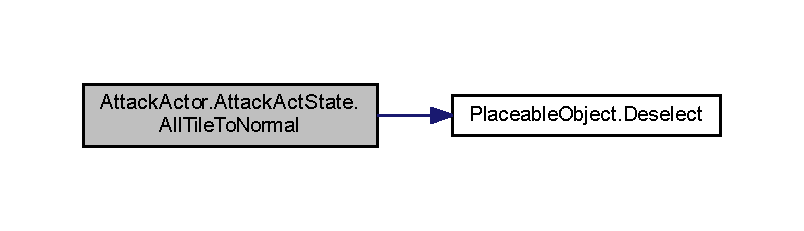
\includegraphics[width=350pt]{class_attack_actor_1_1_attack_act_state_a993762ec959af926e416f03fa7b71203_cgraph}
\end{center}
\end{figure}




이 함수를 호출하는 함수들에 대한 그래프입니다.\+:
\nopagebreak
\begin{figure}[H]
\begin{center}
\leavevmode
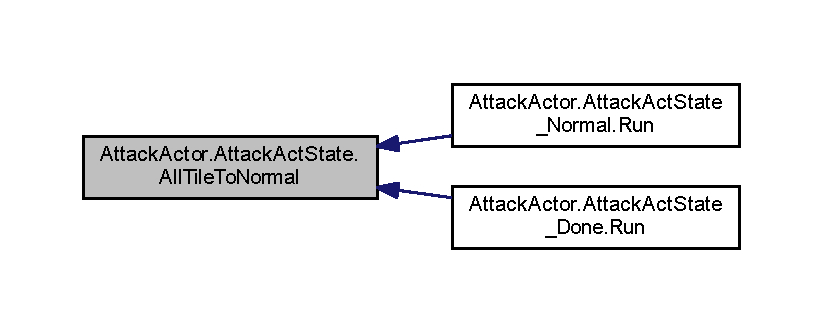
\includegraphics[width=350pt]{class_attack_actor_1_1_attack_act_state_a993762ec959af926e416f03fa7b71203_icgraph}
\end{center}
\end{figure}


\index{Attack\+Actor\+::\+Attack\+Act\+State@{Attack\+Actor\+::\+Attack\+Act\+State}!Destroy@{Destroy}}
\index{Destroy@{Destroy}!Attack\+Actor\+::\+Attack\+Act\+State@{Attack\+Actor\+::\+Attack\+Act\+State}}
\subsubsection[{\texorpdfstring{Destroy()}{Destroy()}}]{\setlength{\rightskip}{0pt plus 5cm}virtual void {\bf M\+C\+N.\+State}$<$ T $>$.Destroy (
\begin{DoxyParamCaption}
{}
\end{DoxyParamCaption}
)\hspace{0.3cm}{\ttfamily [virtual]}, {\ttfamily [inherited]}}\hypertarget{class_m_c_n_1_1_state_a32af22a6a0a979d3b3a80225426aa839}{}\label{class_m_c_n_1_1_state_a32af22a6a0a979d3b3a80225426aa839}


State.\+cs 파일의 47 번째 라인에서 정의되었습니다.


\begin{DoxyCode}
47 \{ \}
\end{DoxyCode}
\index{Attack\+Actor\+::\+Attack\+Act\+State@{Attack\+Actor\+::\+Attack\+Act\+State}!Dispose@{Dispose}}
\index{Dispose@{Dispose}!Attack\+Actor\+::\+Attack\+Act\+State@{Attack\+Actor\+::\+Attack\+Act\+State}}
\subsubsection[{\texorpdfstring{Dispose()}{Dispose()}}]{\setlength{\rightskip}{0pt plus 5cm}void {\bf M\+C\+N.\+State}$<$ T $>$.Dispose (
\begin{DoxyParamCaption}
{}
\end{DoxyParamCaption}
)\hspace{0.3cm}{\ttfamily [inherited]}}\hypertarget{class_m_c_n_1_1_state_a6c53b2eda47e718ff469fd76a95cf02a}{}\label{class_m_c_n_1_1_state_a6c53b2eda47e718ff469fd76a95cf02a}


State.\+cs 파일의 52 번째 라인에서 정의되었습니다.


\begin{DoxyCode}
53         \{
54             \hyperlink{class_m_c_n_1_1_state_ab759357c7d076cf62dd0016b743d762e}{\_target} = \textcolor{keywordflow}{default}(T);
55         \}
\end{DoxyCode}
\index{Attack\+Actor\+::\+Attack\+Act\+State@{Attack\+Actor\+::\+Attack\+Act\+State}!Finish@{Finish}}
\index{Finish@{Finish}!Attack\+Actor\+::\+Attack\+Act\+State@{Attack\+Actor\+::\+Attack\+Act\+State}}
\subsubsection[{\texorpdfstring{Finish()}{Finish()}}]{\setlength{\rightskip}{0pt plus 5cm}virtual void {\bf M\+C\+N.\+State}$<$ T $>$.Finish (
\begin{DoxyParamCaption}
{}
\end{DoxyParamCaption}
)\hspace{0.3cm}{\ttfamily [virtual]}, {\ttfamily [inherited]}}\hypertarget{class_m_c_n_1_1_state_a6de4f94b23916fcd05f589759da9ac3f}{}\label{class_m_c_n_1_1_state_a6de4f94b23916fcd05f589759da9ac3f}


State.\+cs 파일의 50 번째 라인에서 정의되었습니다.


\begin{DoxyCode}
50 \{ \}
\end{DoxyCode}
\index{Attack\+Actor\+::\+Attack\+Act\+State@{Attack\+Actor\+::\+Attack\+Act\+State}!Get\+Current\+Type@{Get\+Current\+Type}}
\index{Get\+Current\+Type@{Get\+Current\+Type}!Attack\+Actor\+::\+Attack\+Act\+State@{Attack\+Actor\+::\+Attack\+Act\+State}}
\subsubsection[{\texorpdfstring{Get\+Current\+Type()}{GetCurrentType()}}]{\setlength{\rightskip}{0pt plus 5cm}abstract {\bf e\+Attack\+Act\+Type} Attack\+Actor.\+Attack\+Act\+State.\+Get\+Current\+Type (
\begin{DoxyParamCaption}
{}
\end{DoxyParamCaption}
)\hspace{0.3cm}{\ttfamily [pure virtual]}}\hypertarget{class_attack_actor_1_1_attack_act_state_a8657ce92996ace441bb68b9e3002aa56}{}\label{class_attack_actor_1_1_attack_act_state_a8657ce92996ace441bb68b9e3002aa56}


\hyperlink{class_attack_actor_1_1_attack_act_state___done_aa72d89d74242db3347ae95f317a6268e}{Attack\+Actor.\+Attack\+Act\+State\+\_\+\+Done}, \hyperlink{class_attack_actor_1_1_attack_act_state___attack_a6622c1356f5d7384b9914bb9611ad285}{Attack\+Actor.\+Attack\+Act\+State\+\_\+\+Attack}, \hyperlink{class_attack_actor_1_1_attack_act_state___normal_a82484dc7be509e6a7a761c3c2b24a64a}{Attack\+Actor.\+Attack\+Act\+State\+\_\+\+Normal}에서 구현되었습니다.



이 함수를 호출하는 함수들에 대한 그래프입니다.\+:
\nopagebreak
\begin{figure}[H]
\begin{center}
\leavevmode
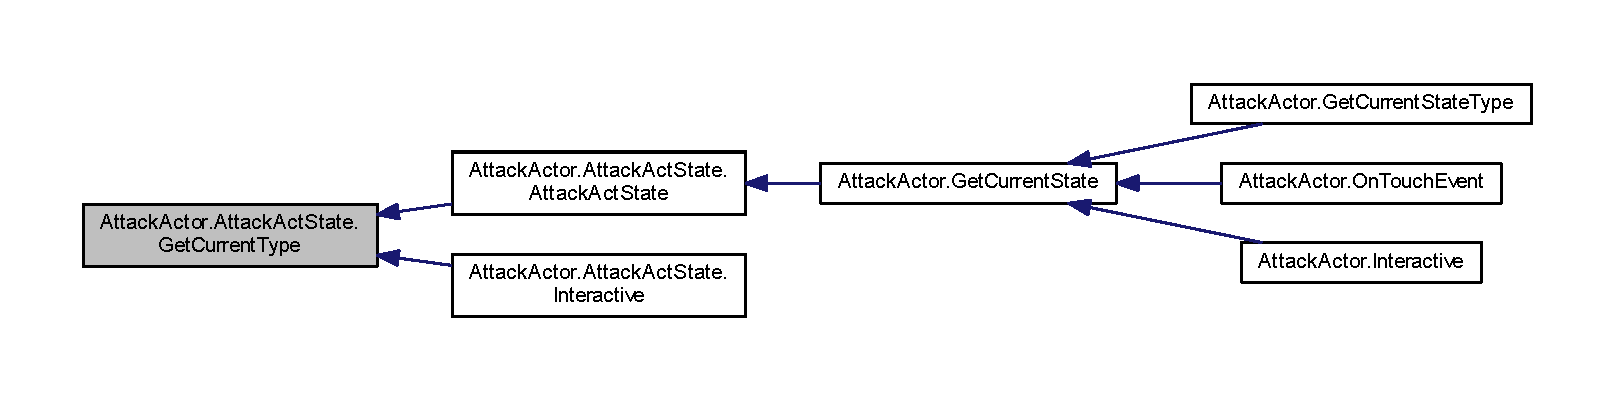
\includegraphics[width=350pt]{class_attack_actor_1_1_attack_act_state_a8657ce92996ace441bb68b9e3002aa56_icgraph}
\end{center}
\end{figure}


\index{Attack\+Actor\+::\+Attack\+Act\+State@{Attack\+Actor\+::\+Attack\+Act\+State}!Initialize@{Initialize}}
\index{Initialize@{Initialize}!Attack\+Actor\+::\+Attack\+Act\+State@{Attack\+Actor\+::\+Attack\+Act\+State}}
\subsubsection[{\texorpdfstring{Initialize()}{Initialize()}}]{\setlength{\rightskip}{0pt plus 5cm}virtual void {\bf M\+C\+N.\+State}$<$ T $>$.Initialize (
\begin{DoxyParamCaption}
{}
\end{DoxyParamCaption}
)\hspace{0.3cm}{\ttfamily [virtual]}, {\ttfamily [inherited]}}\hypertarget{class_m_c_n_1_1_state_a8eabaffe047e6dccd5c5d8aed7bf218a}{}\label{class_m_c_n_1_1_state_a8eabaffe047e6dccd5c5d8aed7bf218a}


State.\+cs 파일의 46 번째 라인에서 정의되었습니다.


\begin{DoxyCode}
46 \{ \}
\end{DoxyCode}
\index{Attack\+Actor\+::\+Attack\+Act\+State@{Attack\+Actor\+::\+Attack\+Act\+State}!Interactive@{Interactive}}
\index{Interactive@{Interactive}!Attack\+Actor\+::\+Attack\+Act\+State@{Attack\+Actor\+::\+Attack\+Act\+State}}
\subsubsection[{\texorpdfstring{Interactive(\+Tile active\+Tile)}{Interactive(Tile activeTile)}}]{\setlength{\rightskip}{0pt plus 5cm}virtual void Attack\+Actor.\+Attack\+Act\+State.\+Interactive (
\begin{DoxyParamCaption}
\item[{{\bf Tile}}]{active\+Tile}
\end{DoxyParamCaption}
)\hspace{0.3cm}{\ttfamily [virtual]}}\hypertarget{class_attack_actor_1_1_attack_act_state_a2ae9dd2f7ec8db76d25d7ad7ed58b89d}{}\label{class_attack_actor_1_1_attack_act_state_a2ae9dd2f7ec8db76d25d7ad7ed58b89d}


\hyperlink{class_attack_actor_1_1_attack_act_state___attack_a59a3f2e994baeddabb870446b5df1641}{Attack\+Actor.\+Attack\+Act\+State\+\_\+\+Attack}에서 재구현되었습니다.



Attack\+Actor.\+cs 파일의 57 번째 라인에서 정의되었습니다.


\begin{DoxyCode}
57 \{ \}
\end{DoxyCode}


이 함수 내부에서 호출하는 함수들에 대한 그래프입니다.\+:
\nopagebreak
\begin{figure}[H]
\begin{center}
\leavevmode
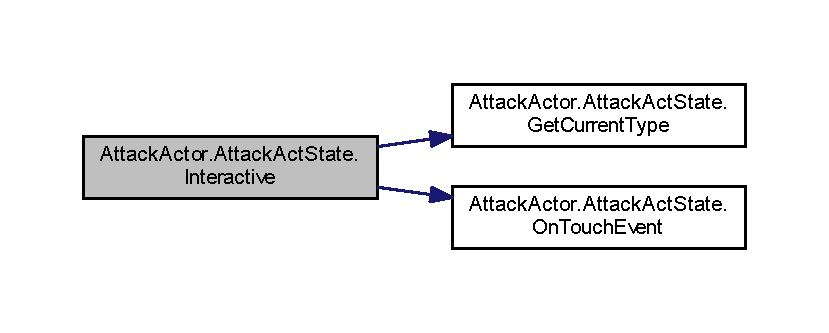
\includegraphics[width=350pt]{class_attack_actor_1_1_attack_act_state_a2ae9dd2f7ec8db76d25d7ad7ed58b89d_cgraph}
\end{center}
\end{figure}


\index{Attack\+Actor\+::\+Attack\+Act\+State@{Attack\+Actor\+::\+Attack\+Act\+State}!On\+Touch\+Event@{On\+Touch\+Event}}
\index{On\+Touch\+Event@{On\+Touch\+Event}!Attack\+Actor\+::\+Attack\+Act\+State@{Attack\+Actor\+::\+Attack\+Act\+State}}
\subsubsection[{\texorpdfstring{On\+Touch\+Event()}{OnTouchEvent()}}]{\setlength{\rightskip}{0pt plus 5cm}abstract bool Attack\+Actor.\+Attack\+Act\+State.\+On\+Touch\+Event (
\begin{DoxyParamCaption}
{}
\end{DoxyParamCaption}
)\hspace{0.3cm}{\ttfamily [pure virtual]}}\hypertarget{class_attack_actor_1_1_attack_act_state_aa5e1794a3ede54c3b71a1463bf5b79a4}{}\label{class_attack_actor_1_1_attack_act_state_aa5e1794a3ede54c3b71a1463bf5b79a4}


\hyperlink{class_attack_actor_1_1_attack_act_state___done_ae982c0e989161fdb1481d799c4e48369}{Attack\+Actor.\+Attack\+Act\+State\+\_\+\+Done}, \hyperlink{class_attack_actor_1_1_attack_act_state___attack_aedb0e05d966cc6b98f92a72f9e5e673a}{Attack\+Actor.\+Attack\+Act\+State\+\_\+\+Attack}, \hyperlink{class_attack_actor_1_1_attack_act_state___normal_ac68685fce5e63f5b1d5fc3e8e74a5621}{Attack\+Actor.\+Attack\+Act\+State\+\_\+\+Normal}에서 구현되었습니다.



이 함수를 호출하는 함수들에 대한 그래프입니다.\+:
\nopagebreak
\begin{figure}[H]
\begin{center}
\leavevmode
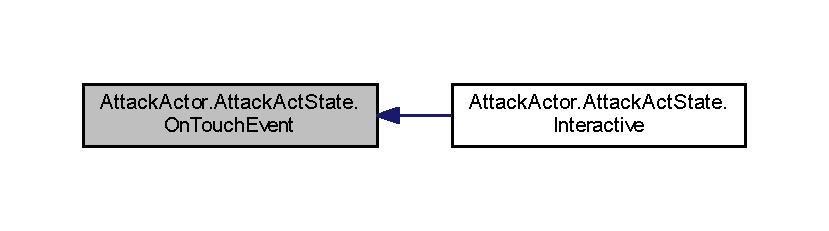
\includegraphics[width=350pt]{class_attack_actor_1_1_attack_act_state_aa5e1794a3ede54c3b71a1463bf5b79a4_icgraph}
\end{center}
\end{figure}


\index{Attack\+Actor\+::\+Attack\+Act\+State@{Attack\+Actor\+::\+Attack\+Act\+State}!Run@{Run}}
\index{Run@{Run}!Attack\+Actor\+::\+Attack\+Act\+State@{Attack\+Actor\+::\+Attack\+Act\+State}}
\subsubsection[{\texorpdfstring{Run()}{Run()}}]{\setlength{\rightskip}{0pt plus 5cm}abstract void {\bf M\+C\+N.\+State}$<$ T $>$.Run (
\begin{DoxyParamCaption}
{}
\end{DoxyParamCaption}
)\hspace{0.3cm}{\ttfamily [pure virtual]}, {\ttfamily [inherited]}}\hypertarget{class_m_c_n_1_1_state_a8adfea67c55997e5c0eefbae1e429f4d}{}\label{class_m_c_n_1_1_state_a8adfea67c55997e5c0eefbae1e429f4d}


\hyperlink{class_attack_actor_1_1_attack_act_state___done_a87dc9fe06b7132e7eff68fce885c2cd2}{Attack\+Actor.\+Attack\+Act\+State\+\_\+\+Done}, \hyperlink{class_attack_actor_1_1_attack_act_state___attack_a2755f4dae2cf1f80a94b6bcc973d1bfd}{Attack\+Actor.\+Attack\+Act\+State\+\_\+\+Attack}, \hyperlink{class_attack_actor_1_1_attack_act_state___normal_a7d6644fed269325b8f62138d8adb50f5}{Attack\+Actor.\+Attack\+Act\+State\+\_\+\+Normal}에서 구현되었습니다.



\subsection{속성 문서화}
\index{Attack\+Actor\+::\+Attack\+Act\+State@{Attack\+Actor\+::\+Attack\+Act\+State}!Target@{Target}}
\index{Target@{Target}!Attack\+Actor\+::\+Attack\+Act\+State@{Attack\+Actor\+::\+Attack\+Act\+State}}
\subsubsection[{\texorpdfstring{Target}{Target}}]{\setlength{\rightskip}{0pt plus 5cm}T {\bf M\+C\+N.\+State}$<$ T $>$.Target\hspace{0.3cm}{\ttfamily [get]}, {\ttfamily [protected]}, {\ttfamily [inherited]}}\hypertarget{class_m_c_n_1_1_state_a93ba2fd920292031bd6e65b1dc505cb3}{}\label{class_m_c_n_1_1_state_a93ba2fd920292031bd6e65b1dc505cb3}


State.\+cs 파일의 32 번째 라인에서 정의되었습니다.



이 클래스에 대한 문서화 페이지는 다음의 파일로부터 생성되었습니다.\+:\begin{DoxyCompactItemize}
\item 
D\+:/\+Git\+Hub/\+M\+C\+N\+Tactics/\+Assets/\+Scripts/\+Objects/\+Actor/\hyperlink{_attack_actor_8cs}{Attack\+Actor.\+cs}\end{DoxyCompactItemize}

\hypertarget{class_attack_actor_1_1_attack_act_state___attack}{}\section{Attack\+Actor.\+Attack\+Act\+State\+\_\+\+Attack 클래스 참조}
\label{class_attack_actor_1_1_attack_act_state___attack}\index{Attack\+Actor.\+Attack\+Act\+State\+\_\+\+Attack@{Attack\+Actor.\+Attack\+Act\+State\+\_\+\+Attack}}


Attack\+Actor.\+Attack\+Act\+State\+\_\+\+Attack에 대한 상속 다이어그램 \+: 
\nopagebreak
\begin{figure}[H]
\begin{center}
\leavevmode
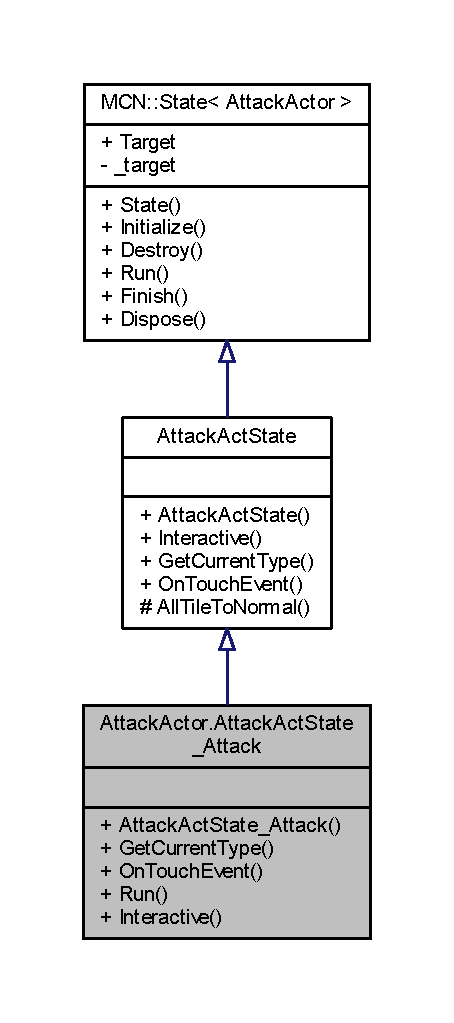
\includegraphics[width=218pt]{class_attack_actor_1_1_attack_act_state___attack__inherit__graph}
\end{center}
\end{figure}


Attack\+Actor.\+Attack\+Act\+State\+\_\+\+Attack에 대한 협력 다이어그램\+:
\nopagebreak
\begin{figure}[H]
\begin{center}
\leavevmode
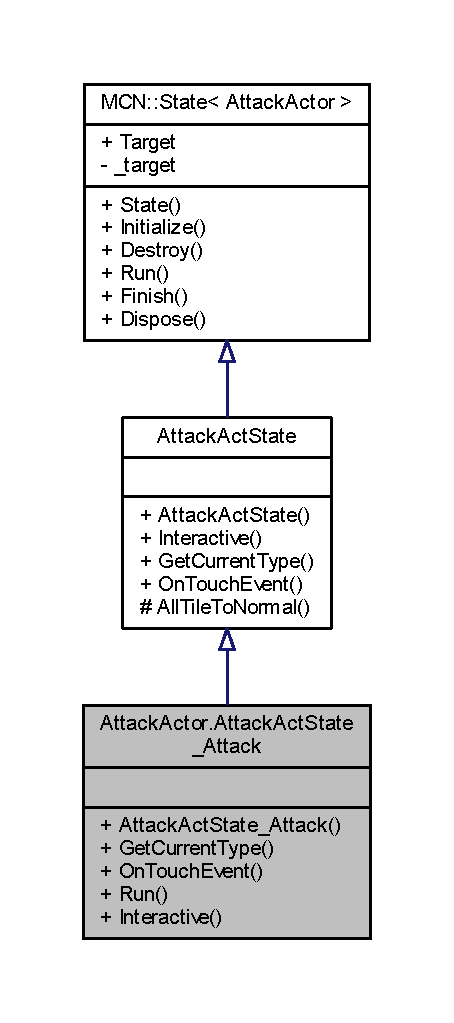
\includegraphics[width=218pt]{class_attack_actor_1_1_attack_act_state___attack__coll__graph}
\end{center}
\end{figure}
\subsection*{Public 멤버 함수}
\begin{DoxyCompactItemize}
\item 
\hyperlink{class_attack_actor_1_1_attack_act_state___attack_a2503cf96e99f943f0be13c3a87e7dd12}{Attack\+Act\+State\+\_\+\+Attack} (\hyperlink{class_attack_actor}{Attack\+Actor} target)
\item 
override \hyperlink{_attack_actor_8cs_a10659ce944335df4ded984f6bc41f31b}{e\+Attack\+Act\+Type} \hyperlink{class_attack_actor_1_1_attack_act_state___attack_a6622c1356f5d7384b9914bb9611ad285}{Get\+Current\+Type} ()
\item 
override bool \hyperlink{class_attack_actor_1_1_attack_act_state___attack_aedb0e05d966cc6b98f92a72f9e5e673a}{On\+Touch\+Event} ()
\item 
override void \hyperlink{class_attack_actor_1_1_attack_act_state___attack_a2755f4dae2cf1f80a94b6bcc973d1bfd}{Run} ()
\item 
override void \hyperlink{class_attack_actor_1_1_attack_act_state___attack_a59a3f2e994baeddabb870446b5df1641}{Interactive} (\hyperlink{class_tile}{Tile} active\+Tile)
\item 
virtual void \hyperlink{class_f_z_1_1_state_a27ac6fd2e844476017b35aa781d73c8c}{Initialize} ()
\item 
virtual void \hyperlink{class_f_z_1_1_state_aa85fdf4a5495d6d5d3ed4aeda3497c8a}{Destroy} ()
\item 
virtual void \hyperlink{class_f_z_1_1_state_a288bb8c3fceee4bf03f01e295dcef1be}{Finish} ()
\item 
void \hyperlink{class_f_z_1_1_state_a598887d3fbb412fada132dc1c079b25b}{Dispose} ()
\end{DoxyCompactItemize}
\subsection*{Protected 멤버 함수}
\begin{DoxyCompactItemize}
\item 
void \hyperlink{class_attack_actor_1_1_attack_act_state_a993762ec959af926e416f03fa7b71203}{All\+Tile\+To\+Normal} ()
\end{DoxyCompactItemize}
\subsection*{속성}
\begin{DoxyCompactItemize}
\item 
T \hyperlink{class_f_z_1_1_state_a6927f5c9f2517052f9dc5596188e9d95}{Target}\hspace{0.3cm}{\ttfamily  \mbox{[}get\mbox{]}}
\end{DoxyCompactItemize}


\subsection{상세한 설명}


Attack\+Actor.\+cs 파일의 100 번째 라인에서 정의되었습니다.



\subsection{생성자 \& 소멸자 문서화}
\index{Attack\+Actor\+::\+Attack\+Act\+State\+\_\+\+Attack@{Attack\+Actor\+::\+Attack\+Act\+State\+\_\+\+Attack}!Attack\+Act\+State\+\_\+\+Attack@{Attack\+Act\+State\+\_\+\+Attack}}
\index{Attack\+Act\+State\+\_\+\+Attack@{Attack\+Act\+State\+\_\+\+Attack}!Attack\+Actor\+::\+Attack\+Act\+State\+\_\+\+Attack@{Attack\+Actor\+::\+Attack\+Act\+State\+\_\+\+Attack}}
\subsubsection[{\texorpdfstring{Attack\+Act\+State\+\_\+\+Attack(\+Attack\+Actor target)}{AttackActState_Attack(AttackActor target)}}]{\setlength{\rightskip}{0pt plus 5cm}Attack\+Actor.\+Attack\+Act\+State\+\_\+\+Attack.\+Attack\+Act\+State\+\_\+\+Attack (
\begin{DoxyParamCaption}
\item[{{\bf Attack\+Actor}}]{target}
\end{DoxyParamCaption}
)}\hypertarget{class_attack_actor_1_1_attack_act_state___attack_a2503cf96e99f943f0be13c3a87e7dd12}{}\label{class_attack_actor_1_1_attack_act_state___attack_a2503cf96e99f943f0be13c3a87e7dd12}


Attack\+Actor.\+cs 파일의 102 번째 라인에서 정의되었습니다.


\begin{DoxyCode}
102 : base(target) \{ \}
\end{DoxyCode}


\subsection{멤버 함수 문서화}
\index{Attack\+Actor\+::\+Attack\+Act\+State\+\_\+\+Attack@{Attack\+Actor\+::\+Attack\+Act\+State\+\_\+\+Attack}!All\+Tile\+To\+Normal@{All\+Tile\+To\+Normal}}
\index{All\+Tile\+To\+Normal@{All\+Tile\+To\+Normal}!Attack\+Actor\+::\+Attack\+Act\+State\+\_\+\+Attack@{Attack\+Actor\+::\+Attack\+Act\+State\+\_\+\+Attack}}
\subsubsection[{\texorpdfstring{All\+Tile\+To\+Normal()}{AllTileToNormal()}}]{\setlength{\rightskip}{0pt plus 5cm}void Attack\+Actor.\+Attack\+Act\+State.\+All\+Tile\+To\+Normal (
\begin{DoxyParamCaption}
{}
\end{DoxyParamCaption}
)\hspace{0.3cm}{\ttfamily [protected]}, {\ttfamily [inherited]}}\hypertarget{class_attack_actor_1_1_attack_act_state_a993762ec959af926e416f03fa7b71203}{}\label{class_attack_actor_1_1_attack_act_state_a993762ec959af926e416f03fa7b71203}


Attack\+Actor.\+cs 파일의 58 번째 라인에서 정의되었습니다.


\begin{DoxyCode}
59         \{
60             \textcolor{keywordflow}{if} (\hyperlink{class_f_z_1_1_state_a6927f5c9f2517052f9dc5596188e9d95}{Target} != null)
61             \{
62                 \hyperlink{class_f_z_1_1_state_a6927f5c9f2517052f9dc5596188e9d95}{Target}.ActTarget.Deselect();
63 
64                 \hyperlink{class_map_manager}{MapManager}.\hyperlink{class_f_z_1_1_mono_singletone_a39e34129d25a9664576949259e7dfd5f}{Instance}.ChangeAllTileState(
      \hyperlink{_tile_8cs_a271bc07be325bca511bcb747e0ff2fda}{eTileType}.NORMAL);
65             \}
66         \}
\end{DoxyCode}


이 함수를 호출하는 함수들에 대한 그래프입니다.\+:\nopagebreak
\begin{figure}[H]
\begin{center}
\leavevmode
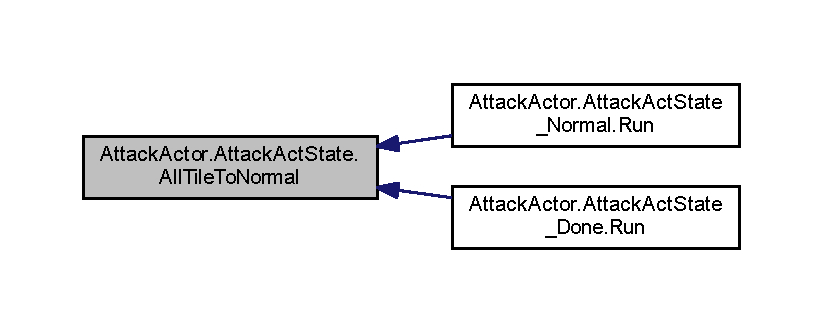
\includegraphics[width=350pt]{class_attack_actor_1_1_attack_act_state_a993762ec959af926e416f03fa7b71203_icgraph}
\end{center}
\end{figure}


\index{Attack\+Actor\+::\+Attack\+Act\+State\+\_\+\+Attack@{Attack\+Actor\+::\+Attack\+Act\+State\+\_\+\+Attack}!Destroy@{Destroy}}
\index{Destroy@{Destroy}!Attack\+Actor\+::\+Attack\+Act\+State\+\_\+\+Attack@{Attack\+Actor\+::\+Attack\+Act\+State\+\_\+\+Attack}}
\subsubsection[{\texorpdfstring{Destroy()}{Destroy()}}]{\setlength{\rightskip}{0pt plus 5cm}virtual void {\bf F\+Z.\+State}$<$ T $>$.Destroy (
\begin{DoxyParamCaption}
{}
\end{DoxyParamCaption}
)\hspace{0.3cm}{\ttfamily [virtual]}, {\ttfamily [inherited]}}\hypertarget{class_f_z_1_1_state_aa85fdf4a5495d6d5d3ed4aeda3497c8a}{}\label{class_f_z_1_1_state_aa85fdf4a5495d6d5d3ed4aeda3497c8a}


State.\+cs 파일의 47 번째 라인에서 정의되었습니다.


\begin{DoxyCode}
47 \{ \}
\end{DoxyCode}
\index{Attack\+Actor\+::\+Attack\+Act\+State\+\_\+\+Attack@{Attack\+Actor\+::\+Attack\+Act\+State\+\_\+\+Attack}!Dispose@{Dispose}}
\index{Dispose@{Dispose}!Attack\+Actor\+::\+Attack\+Act\+State\+\_\+\+Attack@{Attack\+Actor\+::\+Attack\+Act\+State\+\_\+\+Attack}}
\subsubsection[{\texorpdfstring{Dispose()}{Dispose()}}]{\setlength{\rightskip}{0pt plus 5cm}void {\bf F\+Z.\+State}$<$ T $>$.Dispose (
\begin{DoxyParamCaption}
{}
\end{DoxyParamCaption}
)\hspace{0.3cm}{\ttfamily [inherited]}}\hypertarget{class_f_z_1_1_state_a598887d3fbb412fada132dc1c079b25b}{}\label{class_f_z_1_1_state_a598887d3fbb412fada132dc1c079b25b}


State.\+cs 파일의 52 번째 라인에서 정의되었습니다.


\begin{DoxyCode}
53         \{
54             \hyperlink{class_f_z_1_1_state_aff2ae4a7940bd3e363e98e3c0d76d011}{\_target} = \textcolor{keywordflow}{default}(T);
55         \}
\end{DoxyCode}
\index{Attack\+Actor\+::\+Attack\+Act\+State\+\_\+\+Attack@{Attack\+Actor\+::\+Attack\+Act\+State\+\_\+\+Attack}!Finish@{Finish}}
\index{Finish@{Finish}!Attack\+Actor\+::\+Attack\+Act\+State\+\_\+\+Attack@{Attack\+Actor\+::\+Attack\+Act\+State\+\_\+\+Attack}}
\subsubsection[{\texorpdfstring{Finish()}{Finish()}}]{\setlength{\rightskip}{0pt plus 5cm}virtual void {\bf F\+Z.\+State}$<$ T $>$.Finish (
\begin{DoxyParamCaption}
{}
\end{DoxyParamCaption}
)\hspace{0.3cm}{\ttfamily [virtual]}, {\ttfamily [inherited]}}\hypertarget{class_f_z_1_1_state_a288bb8c3fceee4bf03f01e295dcef1be}{}\label{class_f_z_1_1_state_a288bb8c3fceee4bf03f01e295dcef1be}


State.\+cs 파일의 50 번째 라인에서 정의되었습니다.


\begin{DoxyCode}
50 \{ \}
\end{DoxyCode}
\index{Attack\+Actor\+::\+Attack\+Act\+State\+\_\+\+Attack@{Attack\+Actor\+::\+Attack\+Act\+State\+\_\+\+Attack}!Get\+Current\+Type@{Get\+Current\+Type}}
\index{Get\+Current\+Type@{Get\+Current\+Type}!Attack\+Actor\+::\+Attack\+Act\+State\+\_\+\+Attack@{Attack\+Actor\+::\+Attack\+Act\+State\+\_\+\+Attack}}
\subsubsection[{\texorpdfstring{Get\+Current\+Type()}{GetCurrentType()}}]{\setlength{\rightskip}{0pt plus 5cm}override {\bf e\+Attack\+Act\+Type} Attack\+Actor.\+Attack\+Act\+State\+\_\+\+Attack.\+Get\+Current\+Type (
\begin{DoxyParamCaption}
{}
\end{DoxyParamCaption}
)\hspace{0.3cm}{\ttfamily [virtual]}}\hypertarget{class_attack_actor_1_1_attack_act_state___attack_a6622c1356f5d7384b9914bb9611ad285}{}\label{class_attack_actor_1_1_attack_act_state___attack_a6622c1356f5d7384b9914bb9611ad285}


\hyperlink{class_attack_actor_1_1_attack_act_state_a8657ce92996ace441bb68b9e3002aa56}{Attack\+Actor.\+Attack\+Act\+State}를 구현.



Attack\+Actor.\+cs 파일의 104 번째 라인에서 정의되었습니다.


\begin{DoxyCode}
105         \{
106             \textcolor{keywordflow}{return} \hyperlink{_attack_actor_8cs_a10659ce944335df4ded984f6bc41f31b}{eAttackActType}.ATTACK;
107         \}
\end{DoxyCode}
\index{Attack\+Actor\+::\+Attack\+Act\+State\+\_\+\+Attack@{Attack\+Actor\+::\+Attack\+Act\+State\+\_\+\+Attack}!Initialize@{Initialize}}
\index{Initialize@{Initialize}!Attack\+Actor\+::\+Attack\+Act\+State\+\_\+\+Attack@{Attack\+Actor\+::\+Attack\+Act\+State\+\_\+\+Attack}}
\subsubsection[{\texorpdfstring{Initialize()}{Initialize()}}]{\setlength{\rightskip}{0pt plus 5cm}virtual void {\bf F\+Z.\+State}$<$ T $>$.Initialize (
\begin{DoxyParamCaption}
{}
\end{DoxyParamCaption}
)\hspace{0.3cm}{\ttfamily [virtual]}, {\ttfamily [inherited]}}\hypertarget{class_f_z_1_1_state_a27ac6fd2e844476017b35aa781d73c8c}{}\label{class_f_z_1_1_state_a27ac6fd2e844476017b35aa781d73c8c}


State.\+cs 파일의 46 번째 라인에서 정의되었습니다.


\begin{DoxyCode}
46 \{ \}
\end{DoxyCode}
\index{Attack\+Actor\+::\+Attack\+Act\+State\+\_\+\+Attack@{Attack\+Actor\+::\+Attack\+Act\+State\+\_\+\+Attack}!Interactive@{Interactive}}
\index{Interactive@{Interactive}!Attack\+Actor\+::\+Attack\+Act\+State\+\_\+\+Attack@{Attack\+Actor\+::\+Attack\+Act\+State\+\_\+\+Attack}}
\subsubsection[{\texorpdfstring{Interactive(\+Tile active\+Tile)}{Interactive(Tile activeTile)}}]{\setlength{\rightskip}{0pt plus 5cm}override void Attack\+Actor.\+Attack\+Act\+State\+\_\+\+Attack.\+Interactive (
\begin{DoxyParamCaption}
\item[{{\bf Tile}}]{active\+Tile}
\end{DoxyParamCaption}
)\hspace{0.3cm}{\ttfamily [virtual]}}\hypertarget{class_attack_actor_1_1_attack_act_state___attack_a59a3f2e994baeddabb870446b5df1641}{}\label{class_attack_actor_1_1_attack_act_state___attack_a59a3f2e994baeddabb870446b5df1641}


\hyperlink{class_attack_actor_1_1_attack_act_state_a2ae9dd2f7ec8db76d25d7ad7ed58b89d}{Attack\+Actor.\+Attack\+Act\+State}(으)로부터 재구현되었습니다.



Attack\+Actor.\+cs 파일의 145 번째 라인에서 정의되었습니다.


\begin{DoxyCode}
146         \{
147             \textcolor{keywordflow}{if} (\hyperlink{class_f_z_1_1_state_a6927f5c9f2517052f9dc5596188e9d95}{Target} != null)
148             \{
149                 var damagedTarget = activeTile.\hyperlink{class_tile_a955e550fb4df0be4245223e9520c9559}{GetAttachObject}() as 
      \hyperlink{class_unit_object}{UnitObject};
150 
151                 \textcolor{keywordflow}{if} (damagedTarget != null)
152                 \{
153                     damagedTarget.\hyperlink{class_unit_object_a36511c5c48346ec7aba58e0150b3d462}{Damaged}(\hyperlink{class_f_z_1_1_state_a6927f5c9f2517052f9dc5596188e9d95}{Target});
154 
155                     \hyperlink{class_f_z_1_1_state_a6927f5c9f2517052f9dc5596188e9d95}{Target}.ChangeState(\hyperlink{_attack_actor_8cs_a10659ce944335df4ded984f6bc41f31b}{eAttackActType}.DONE);
156                 \}
157             \}
158         \}
\end{DoxyCode}


이 함수 내부에서 호출하는 함수들에 대한 그래프입니다.\+:
\nopagebreak
\begin{figure}[H]
\begin{center}
\leavevmode
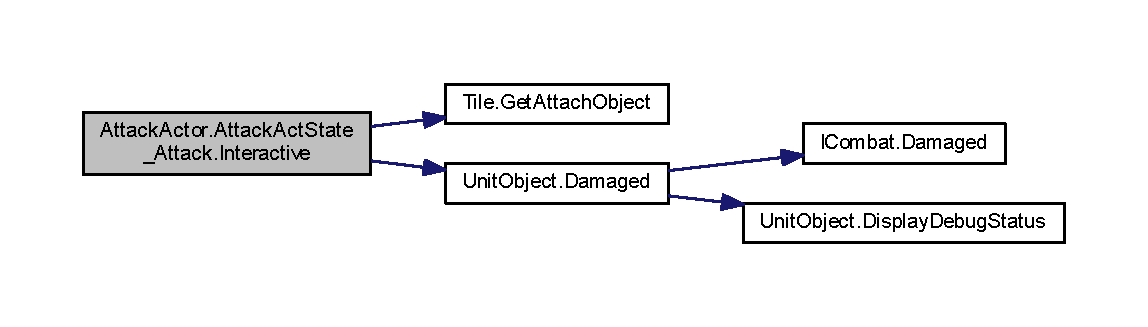
\includegraphics[width=350pt]{class_attack_actor_1_1_attack_act_state___attack_a59a3f2e994baeddabb870446b5df1641_cgraph}
\end{center}
\end{figure}


\index{Attack\+Actor\+::\+Attack\+Act\+State\+\_\+\+Attack@{Attack\+Actor\+::\+Attack\+Act\+State\+\_\+\+Attack}!On\+Touch\+Event@{On\+Touch\+Event}}
\index{On\+Touch\+Event@{On\+Touch\+Event}!Attack\+Actor\+::\+Attack\+Act\+State\+\_\+\+Attack@{Attack\+Actor\+::\+Attack\+Act\+State\+\_\+\+Attack}}
\subsubsection[{\texorpdfstring{On\+Touch\+Event()}{OnTouchEvent()}}]{\setlength{\rightskip}{0pt plus 5cm}override bool Attack\+Actor.\+Attack\+Act\+State\+\_\+\+Attack.\+On\+Touch\+Event (
\begin{DoxyParamCaption}
{}
\end{DoxyParamCaption}
)\hspace{0.3cm}{\ttfamily [virtual]}}\hypertarget{class_attack_actor_1_1_attack_act_state___attack_aedb0e05d966cc6b98f92a72f9e5e673a}{}\label{class_attack_actor_1_1_attack_act_state___attack_aedb0e05d966cc6b98f92a72f9e5e673a}


\hyperlink{class_attack_actor_1_1_attack_act_state_aa5e1794a3ede54c3b71a1463bf5b79a4}{Attack\+Actor.\+Attack\+Act\+State}를 구현.



Attack\+Actor.\+cs 파일의 109 번째 라인에서 정의되었습니다.


\begin{DoxyCode}
110         \{
111             \textcolor{keywordflow}{if} (\hyperlink{class_f_z_1_1_state_a6927f5c9f2517052f9dc5596188e9d95}{Target} != null)
112             \{
113                 \textcolor{keywordflow}{if} (\hyperlink{class_f_z_1_1_state_a6927f5c9f2517052f9dc5596188e9d95}{Target}.ActTarget.IsSelected())
114                 \{
115                     \hyperlink{class_f_z_1_1_state_a6927f5c9f2517052f9dc5596188e9d95}{Target}.ChangeState(\hyperlink{_attack_actor_8cs_a10659ce944335df4ded984f6bc41f31b}{eAttackActType}.NORMAL);
116                 \}
117             \}
118 
119             \textcolor{keywordflow}{return} \textcolor{keyword}{false};
120         \}
\end{DoxyCode}
\index{Attack\+Actor\+::\+Attack\+Act\+State\+\_\+\+Attack@{Attack\+Actor\+::\+Attack\+Act\+State\+\_\+\+Attack}!Run@{Run}}
\index{Run@{Run}!Attack\+Actor\+::\+Attack\+Act\+State\+\_\+\+Attack@{Attack\+Actor\+::\+Attack\+Act\+State\+\_\+\+Attack}}
\subsubsection[{\texorpdfstring{Run()}{Run()}}]{\setlength{\rightskip}{0pt plus 5cm}override void Attack\+Actor.\+Attack\+Act\+State\+\_\+\+Attack.\+Run (
\begin{DoxyParamCaption}
{}
\end{DoxyParamCaption}
)\hspace{0.3cm}{\ttfamily [virtual]}}\hypertarget{class_attack_actor_1_1_attack_act_state___attack_a2755f4dae2cf1f80a94b6bcc973d1bfd}{}\label{class_attack_actor_1_1_attack_act_state___attack_a2755f4dae2cf1f80a94b6bcc973d1bfd}


\hyperlink{class_f_z_1_1_state_acaf1584680a2e69e2a4da20574723981}{F\+Z.\+State$<$ Attack\+Actor $>$}를 구현.



Attack\+Actor.\+cs 파일의 122 번째 라인에서 정의되었습니다.


\begin{DoxyCode}
123         \{
124             \textcolor{keywordflow}{if} (\hyperlink{class_f_z_1_1_state_a6927f5c9f2517052f9dc5596188e9d95}{Target} != null)
125             \{
126                 \hyperlink{class_f_z_1_1_state_a6927f5c9f2517052f9dc5596188e9d95}{Target}.ActTarget.Select();
127 
128                 \textcolor{keywordflow}{if} (\hyperlink{class_f_z_1_1_state_a6927f5c9f2517052f9dc5596188e9d95}{Target}.ActTarget.GetPlacedTile() != null)
129                 \{
130                     \hyperlink{class_map_manager}{MapManager}.\hyperlink{class_f_z_1_1_mono_singletone_a39e34129d25a9664576949259e7dfd5f}{Instance}.ChangeAllTileState(
      \hyperlink{_tile_8cs_a271bc07be325bca511bcb747e0ff2fda}{eTileType}.DEACTIVE);
131 
132                     var placedTile = \hyperlink{class_f_z_1_1_state_a6927f5c9f2517052f9dc5596188e9d95}{Target}.ActTarget.GetPlacedTile();
133 
134                     Func<Tile, bool> tileDeactiveCond = (\hyperlink{class_tile}{Tile} tile) =>
135                     \{
136                         \textcolor{keywordflow}{return} (tile.GetAttachObject() != null && !(tile.GetAttachObject() is 
      \hyperlink{class_unit_object}{UnitObject})) ||
137                                (tile.GetAttachObject() is \hyperlink{class_unit_object}{UnitObject} && (tile.GetAttachObject() 
      as \hyperlink{class_unit_object}{UnitObject}).Team == \hyperlink{class_f_z_1_1_state_a6927f5c9f2517052f9dc5596188e9d95}{Target}.ActTarget.Team);
138                     \};
139 
140                     placedTile.ShowChainActiveTile(\hyperlink{class_f_z_1_1_state_a6927f5c9f2517052f9dc5596188e9d95}{Target}.Range, tileDeactiveCond);
141                 \}
142             \}
143         \}
\end{DoxyCode}


\subsection{속성 문서화}
\index{Attack\+Actor\+::\+Attack\+Act\+State\+\_\+\+Attack@{Attack\+Actor\+::\+Attack\+Act\+State\+\_\+\+Attack}!Target@{Target}}
\index{Target@{Target}!Attack\+Actor\+::\+Attack\+Act\+State\+\_\+\+Attack@{Attack\+Actor\+::\+Attack\+Act\+State\+\_\+\+Attack}}
\subsubsection[{\texorpdfstring{Target}{Target}}]{\setlength{\rightskip}{0pt plus 5cm}T {\bf F\+Z.\+State}$<$ T $>$.Target\hspace{0.3cm}{\ttfamily [get]}, {\ttfamily [protected]}, {\ttfamily [inherited]}}\hypertarget{class_f_z_1_1_state_a6927f5c9f2517052f9dc5596188e9d95}{}\label{class_f_z_1_1_state_a6927f5c9f2517052f9dc5596188e9d95}


State.\+cs 파일의 32 번째 라인에서 정의되었습니다.



이 클래스에 대한 문서화 페이지는 다음의 파일로부터 생성되었습니다.\+:\begin{DoxyCompactItemize}
\item 
D\+:/\+Git\+Hub/\+M\+C\+N\+Tactics/\+Assets/\+Scripts/\+Objects/\+Actor/\hyperlink{_attack_actor_8cs}{Attack\+Actor.\+cs}\end{DoxyCompactItemize}

\hypertarget{class_attack_actor_1_1_attack_act_state___done}{}\section{Attack\+Actor.\+Attack\+Act\+State\+\_\+\+Done 클래스 참조}
\label{class_attack_actor_1_1_attack_act_state___done}\index{Attack\+Actor.\+Attack\+Act\+State\+\_\+\+Done@{Attack\+Actor.\+Attack\+Act\+State\+\_\+\+Done}}


Attack\+Actor.\+Attack\+Act\+State\+\_\+\+Done에 대한 상속 다이어그램 \+: 
\nopagebreak
\begin{figure}[H]
\begin{center}
\leavevmode
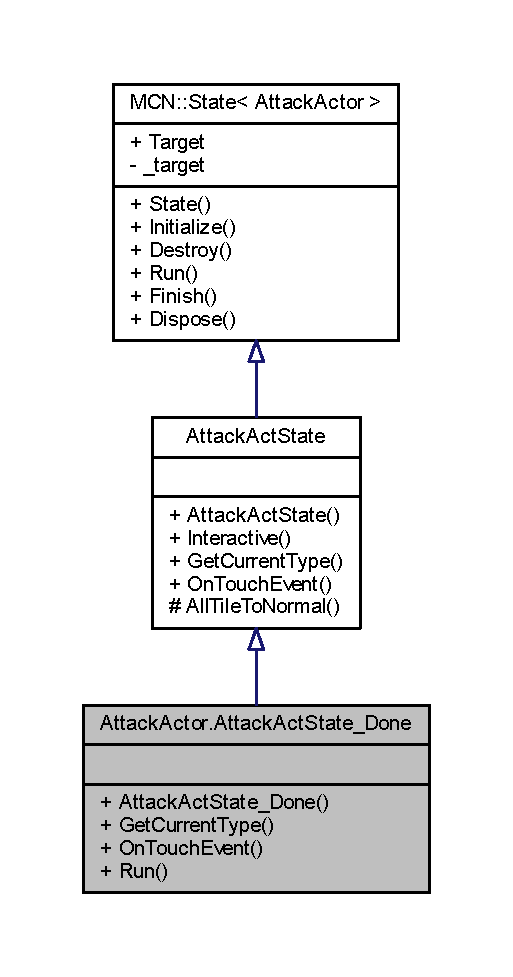
\includegraphics[width=246pt]{class_attack_actor_1_1_attack_act_state___done__inherit__graph}
\end{center}
\end{figure}


Attack\+Actor.\+Attack\+Act\+State\+\_\+\+Done에 대한 협력 다이어그램\+:
\nopagebreak
\begin{figure}[H]
\begin{center}
\leavevmode
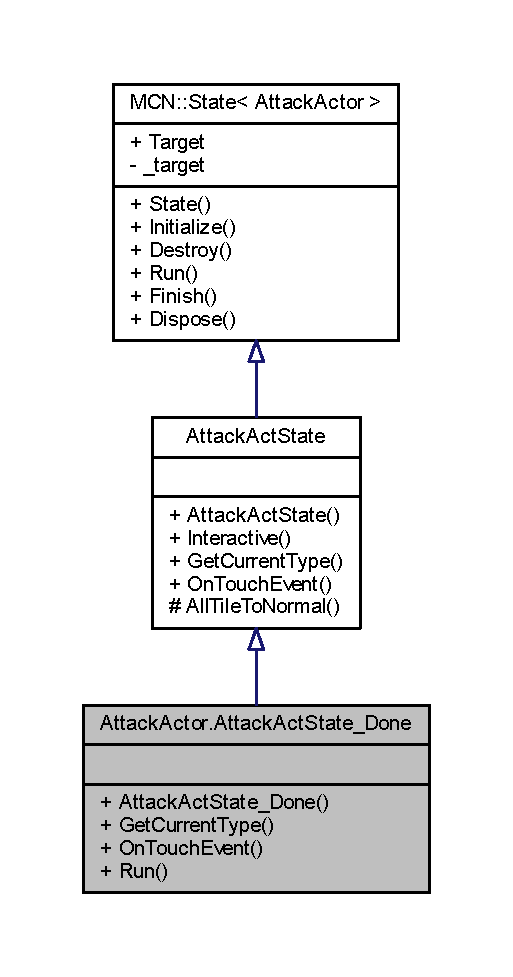
\includegraphics[width=246pt]{class_attack_actor_1_1_attack_act_state___done__coll__graph}
\end{center}
\end{figure}
\subsection*{Public 멤버 함수}
\begin{DoxyCompactItemize}
\item 
\hyperlink{class_attack_actor_1_1_attack_act_state___done_a57cc20f4a46c32a80eed29122c71c2e0}{Attack\+Act\+State\+\_\+\+Done} (\hyperlink{class_attack_actor}{Attack\+Actor} target)
\item 
override \hyperlink{_attack_actor_8cs_a10659ce944335df4ded984f6bc41f31b}{e\+Attack\+Act\+Type} \hyperlink{class_attack_actor_1_1_attack_act_state___done_aa72d89d74242db3347ae95f317a6268e}{Get\+Current\+Type} ()
\item 
override bool \hyperlink{class_attack_actor_1_1_attack_act_state___done_ae982c0e989161fdb1481d799c4e48369}{On\+Touch\+Event} ()
\item 
override void \hyperlink{class_attack_actor_1_1_attack_act_state___done_a87dc9fe06b7132e7eff68fce885c2cd2}{Run} ()
\item 
virtual void \hyperlink{class_attack_actor_1_1_attack_act_state_a2ae9dd2f7ec8db76d25d7ad7ed58b89d}{Interactive} (\hyperlink{class_tile}{Tile} active\+Tile)
\item 
virtual void \hyperlink{class_m_c_n_1_1_state_a8eabaffe047e6dccd5c5d8aed7bf218a}{Initialize} ()
\item 
virtual void \hyperlink{class_m_c_n_1_1_state_a32af22a6a0a979d3b3a80225426aa839}{Destroy} ()
\item 
virtual void \hyperlink{class_m_c_n_1_1_state_a6de4f94b23916fcd05f589759da9ac3f}{Finish} ()
\item 
void \hyperlink{class_m_c_n_1_1_state_a6c53b2eda47e718ff469fd76a95cf02a}{Dispose} ()
\end{DoxyCompactItemize}
\subsection*{Protected 멤버 함수}
\begin{DoxyCompactItemize}
\item 
void \hyperlink{class_attack_actor_1_1_attack_act_state_a993762ec959af926e416f03fa7b71203}{All\+Tile\+To\+Normal} ()
\end{DoxyCompactItemize}
\subsection*{속성}
\begin{DoxyCompactItemize}
\item 
T \hyperlink{class_m_c_n_1_1_state_a93ba2fd920292031bd6e65b1dc505cb3}{Target}\hspace{0.3cm}{\ttfamily  \mbox{[}get\mbox{]}}
\end{DoxyCompactItemize}


\subsection{상세한 설명}


Attack\+Actor.\+cs 파일의 176 번째 라인에서 정의되었습니다.



\subsection{생성자 \& 소멸자 문서화}
\index{Attack\+Actor\+::\+Attack\+Act\+State\+\_\+\+Done@{Attack\+Actor\+::\+Attack\+Act\+State\+\_\+\+Done}!Attack\+Act\+State\+\_\+\+Done@{Attack\+Act\+State\+\_\+\+Done}}
\index{Attack\+Act\+State\+\_\+\+Done@{Attack\+Act\+State\+\_\+\+Done}!Attack\+Actor\+::\+Attack\+Act\+State\+\_\+\+Done@{Attack\+Actor\+::\+Attack\+Act\+State\+\_\+\+Done}}
\subsubsection[{\texorpdfstring{Attack\+Act\+State\+\_\+\+Done(\+Attack\+Actor target)}{AttackActState_Done(AttackActor target)}}]{\setlength{\rightskip}{0pt plus 5cm}Attack\+Actor.\+Attack\+Act\+State\+\_\+\+Done.\+Attack\+Act\+State\+\_\+\+Done (
\begin{DoxyParamCaption}
\item[{{\bf Attack\+Actor}}]{target}
\end{DoxyParamCaption}
)}\hypertarget{class_attack_actor_1_1_attack_act_state___done_a57cc20f4a46c32a80eed29122c71c2e0}{}\label{class_attack_actor_1_1_attack_act_state___done_a57cc20f4a46c32a80eed29122c71c2e0}


Attack\+Actor.\+cs 파일의 178 번째 라인에서 정의되었습니다.


\begin{DoxyCode}
178 : base(target) \{ \}
\end{DoxyCode}


\subsection{멤버 함수 문서화}
\index{Attack\+Actor\+::\+Attack\+Act\+State\+\_\+\+Done@{Attack\+Actor\+::\+Attack\+Act\+State\+\_\+\+Done}!All\+Tile\+To\+Normal@{All\+Tile\+To\+Normal}}
\index{All\+Tile\+To\+Normal@{All\+Tile\+To\+Normal}!Attack\+Actor\+::\+Attack\+Act\+State\+\_\+\+Done@{Attack\+Actor\+::\+Attack\+Act\+State\+\_\+\+Done}}
\subsubsection[{\texorpdfstring{All\+Tile\+To\+Normal()}{AllTileToNormal()}}]{\setlength{\rightskip}{0pt plus 5cm}void Attack\+Actor.\+Attack\+Act\+State.\+All\+Tile\+To\+Normal (
\begin{DoxyParamCaption}
{}
\end{DoxyParamCaption}
)\hspace{0.3cm}{\ttfamily [protected]}, {\ttfamily [inherited]}}\hypertarget{class_attack_actor_1_1_attack_act_state_a993762ec959af926e416f03fa7b71203}{}\label{class_attack_actor_1_1_attack_act_state_a993762ec959af926e416f03fa7b71203}


Attack\+Actor.\+cs 파일의 63 번째 라인에서 정의되었습니다.


\begin{DoxyCode}
64         \{
65             \textcolor{keywordflow}{if} (\hyperlink{class_m_c_n_1_1_state_a93ba2fd920292031bd6e65b1dc505cb3}{Target} != null)
66             \{
67                 var placeable = \hyperlink{class_m_c_n_1_1_state_a93ba2fd920292031bd6e65b1dc505cb3}{Target}.ActTarget as \hyperlink{class_placeable_object}{PlaceableObject};
68 
69                 \textcolor{keywordflow}{if} (placeable != null)
70                 \{
71                     placeable.\hyperlink{class_placeable_object_a0c1248b1f9981ddbf68e6f70a6498f3d}{Deselect}();
72 
73                     \hyperlink{class_map_manager}{MapManager}.\hyperlink{class_m_c_n_1_1_mono_singletone_aa50c027cca64cf4ad30c1ee5c83e0b78}{Instance}.ChangeAllTileState(
      \hyperlink{_tile_8cs_a271bc07be325bca511bcb747e0ff2fda}{eTileType}.NORMAL);
74                 \}
75             \}
76         \}
\end{DoxyCode}


이 함수 내부에서 호출하는 함수들에 대한 그래프입니다.\+:
\nopagebreak
\begin{figure}[H]
\begin{center}
\leavevmode
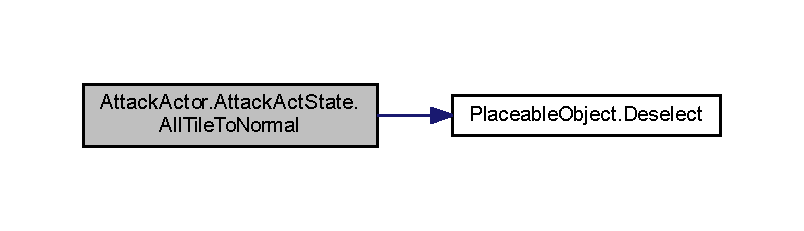
\includegraphics[width=350pt]{class_attack_actor_1_1_attack_act_state_a993762ec959af926e416f03fa7b71203_cgraph}
\end{center}
\end{figure}




이 함수를 호출하는 함수들에 대한 그래프입니다.\+:
\nopagebreak
\begin{figure}[H]
\begin{center}
\leavevmode
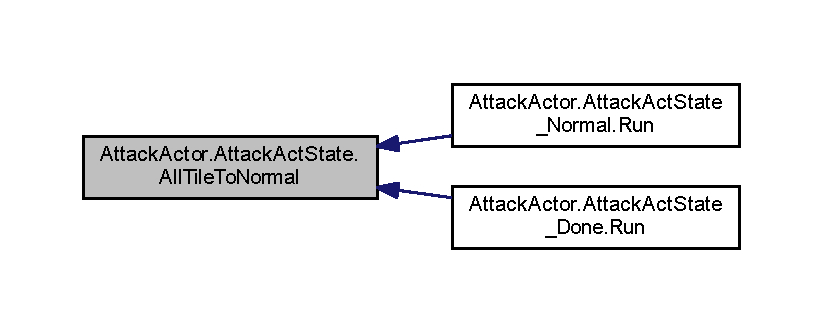
\includegraphics[width=350pt]{class_attack_actor_1_1_attack_act_state_a993762ec959af926e416f03fa7b71203_icgraph}
\end{center}
\end{figure}


\index{Attack\+Actor\+::\+Attack\+Act\+State\+\_\+\+Done@{Attack\+Actor\+::\+Attack\+Act\+State\+\_\+\+Done}!Destroy@{Destroy}}
\index{Destroy@{Destroy}!Attack\+Actor\+::\+Attack\+Act\+State\+\_\+\+Done@{Attack\+Actor\+::\+Attack\+Act\+State\+\_\+\+Done}}
\subsubsection[{\texorpdfstring{Destroy()}{Destroy()}}]{\setlength{\rightskip}{0pt plus 5cm}virtual void {\bf M\+C\+N.\+State}$<$ T $>$.Destroy (
\begin{DoxyParamCaption}
{}
\end{DoxyParamCaption}
)\hspace{0.3cm}{\ttfamily [virtual]}, {\ttfamily [inherited]}}\hypertarget{class_m_c_n_1_1_state_a32af22a6a0a979d3b3a80225426aa839}{}\label{class_m_c_n_1_1_state_a32af22a6a0a979d3b3a80225426aa839}


State.\+cs 파일의 47 번째 라인에서 정의되었습니다.


\begin{DoxyCode}
47 \{ \}
\end{DoxyCode}
\index{Attack\+Actor\+::\+Attack\+Act\+State\+\_\+\+Done@{Attack\+Actor\+::\+Attack\+Act\+State\+\_\+\+Done}!Dispose@{Dispose}}
\index{Dispose@{Dispose}!Attack\+Actor\+::\+Attack\+Act\+State\+\_\+\+Done@{Attack\+Actor\+::\+Attack\+Act\+State\+\_\+\+Done}}
\subsubsection[{\texorpdfstring{Dispose()}{Dispose()}}]{\setlength{\rightskip}{0pt plus 5cm}void {\bf M\+C\+N.\+State}$<$ T $>$.Dispose (
\begin{DoxyParamCaption}
{}
\end{DoxyParamCaption}
)\hspace{0.3cm}{\ttfamily [inherited]}}\hypertarget{class_m_c_n_1_1_state_a6c53b2eda47e718ff469fd76a95cf02a}{}\label{class_m_c_n_1_1_state_a6c53b2eda47e718ff469fd76a95cf02a}


State.\+cs 파일의 52 번째 라인에서 정의되었습니다.


\begin{DoxyCode}
53         \{
54             \hyperlink{class_m_c_n_1_1_state_ab759357c7d076cf62dd0016b743d762e}{\_target} = \textcolor{keywordflow}{default}(T);
55         \}
\end{DoxyCode}
\index{Attack\+Actor\+::\+Attack\+Act\+State\+\_\+\+Done@{Attack\+Actor\+::\+Attack\+Act\+State\+\_\+\+Done}!Finish@{Finish}}
\index{Finish@{Finish}!Attack\+Actor\+::\+Attack\+Act\+State\+\_\+\+Done@{Attack\+Actor\+::\+Attack\+Act\+State\+\_\+\+Done}}
\subsubsection[{\texorpdfstring{Finish()}{Finish()}}]{\setlength{\rightskip}{0pt plus 5cm}virtual void {\bf M\+C\+N.\+State}$<$ T $>$.Finish (
\begin{DoxyParamCaption}
{}
\end{DoxyParamCaption}
)\hspace{0.3cm}{\ttfamily [virtual]}, {\ttfamily [inherited]}}\hypertarget{class_m_c_n_1_1_state_a6de4f94b23916fcd05f589759da9ac3f}{}\label{class_m_c_n_1_1_state_a6de4f94b23916fcd05f589759da9ac3f}


State.\+cs 파일의 50 번째 라인에서 정의되었습니다.


\begin{DoxyCode}
50 \{ \}
\end{DoxyCode}
\index{Attack\+Actor\+::\+Attack\+Act\+State\+\_\+\+Done@{Attack\+Actor\+::\+Attack\+Act\+State\+\_\+\+Done}!Get\+Current\+Type@{Get\+Current\+Type}}
\index{Get\+Current\+Type@{Get\+Current\+Type}!Attack\+Actor\+::\+Attack\+Act\+State\+\_\+\+Done@{Attack\+Actor\+::\+Attack\+Act\+State\+\_\+\+Done}}
\subsubsection[{\texorpdfstring{Get\+Current\+Type()}{GetCurrentType()}}]{\setlength{\rightskip}{0pt plus 5cm}override {\bf e\+Attack\+Act\+Type} Attack\+Actor.\+Attack\+Act\+State\+\_\+\+Done.\+Get\+Current\+Type (
\begin{DoxyParamCaption}
{}
\end{DoxyParamCaption}
)\hspace{0.3cm}{\ttfamily [virtual]}}\hypertarget{class_attack_actor_1_1_attack_act_state___done_aa72d89d74242db3347ae95f317a6268e}{}\label{class_attack_actor_1_1_attack_act_state___done_aa72d89d74242db3347ae95f317a6268e}


\hyperlink{class_attack_actor_1_1_attack_act_state_a8657ce92996ace441bb68b9e3002aa56}{Attack\+Actor.\+Attack\+Act\+State}를 구현.



Attack\+Actor.\+cs 파일의 180 번째 라인에서 정의되었습니다.


\begin{DoxyCode}
181         \{
182             \textcolor{keywordflow}{return} \hyperlink{_attack_actor_8cs_a10659ce944335df4ded984f6bc41f31b}{eAttackActType}.DONE;
183         \}
\end{DoxyCode}
\index{Attack\+Actor\+::\+Attack\+Act\+State\+\_\+\+Done@{Attack\+Actor\+::\+Attack\+Act\+State\+\_\+\+Done}!Initialize@{Initialize}}
\index{Initialize@{Initialize}!Attack\+Actor\+::\+Attack\+Act\+State\+\_\+\+Done@{Attack\+Actor\+::\+Attack\+Act\+State\+\_\+\+Done}}
\subsubsection[{\texorpdfstring{Initialize()}{Initialize()}}]{\setlength{\rightskip}{0pt plus 5cm}virtual void {\bf M\+C\+N.\+State}$<$ T $>$.Initialize (
\begin{DoxyParamCaption}
{}
\end{DoxyParamCaption}
)\hspace{0.3cm}{\ttfamily [virtual]}, {\ttfamily [inherited]}}\hypertarget{class_m_c_n_1_1_state_a8eabaffe047e6dccd5c5d8aed7bf218a}{}\label{class_m_c_n_1_1_state_a8eabaffe047e6dccd5c5d8aed7bf218a}


State.\+cs 파일의 46 번째 라인에서 정의되었습니다.


\begin{DoxyCode}
46 \{ \}
\end{DoxyCode}
\index{Attack\+Actor\+::\+Attack\+Act\+State\+\_\+\+Done@{Attack\+Actor\+::\+Attack\+Act\+State\+\_\+\+Done}!Interactive@{Interactive}}
\index{Interactive@{Interactive}!Attack\+Actor\+::\+Attack\+Act\+State\+\_\+\+Done@{Attack\+Actor\+::\+Attack\+Act\+State\+\_\+\+Done}}
\subsubsection[{\texorpdfstring{Interactive(\+Tile active\+Tile)}{Interactive(Tile activeTile)}}]{\setlength{\rightskip}{0pt plus 5cm}virtual void Attack\+Actor.\+Attack\+Act\+State.\+Interactive (
\begin{DoxyParamCaption}
\item[{{\bf Tile}}]{active\+Tile}
\end{DoxyParamCaption}
)\hspace{0.3cm}{\ttfamily [virtual]}, {\ttfamily [inherited]}}\hypertarget{class_attack_actor_1_1_attack_act_state_a2ae9dd2f7ec8db76d25d7ad7ed58b89d}{}\label{class_attack_actor_1_1_attack_act_state_a2ae9dd2f7ec8db76d25d7ad7ed58b89d}


\hyperlink{class_attack_actor_1_1_attack_act_state___attack_a59a3f2e994baeddabb870446b5df1641}{Attack\+Actor.\+Attack\+Act\+State\+\_\+\+Attack}에서 재구현되었습니다.



Attack\+Actor.\+cs 파일의 57 번째 라인에서 정의되었습니다.


\begin{DoxyCode}
57 \{ \}
\end{DoxyCode}


이 함수 내부에서 호출하는 함수들에 대한 그래프입니다.\+:
\nopagebreak
\begin{figure}[H]
\begin{center}
\leavevmode
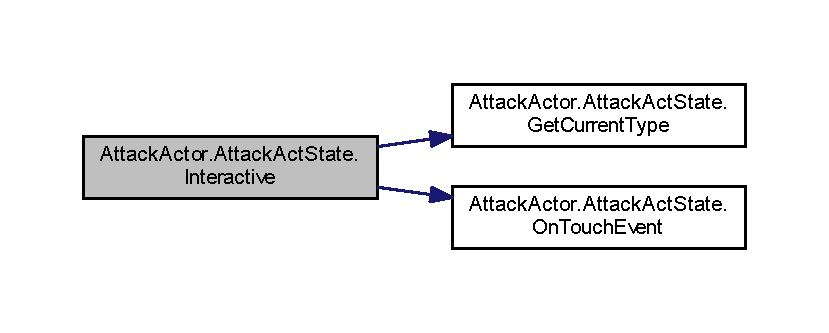
\includegraphics[width=350pt]{class_attack_actor_1_1_attack_act_state_a2ae9dd2f7ec8db76d25d7ad7ed58b89d_cgraph}
\end{center}
\end{figure}


\index{Attack\+Actor\+::\+Attack\+Act\+State\+\_\+\+Done@{Attack\+Actor\+::\+Attack\+Act\+State\+\_\+\+Done}!On\+Touch\+Event@{On\+Touch\+Event}}
\index{On\+Touch\+Event@{On\+Touch\+Event}!Attack\+Actor\+::\+Attack\+Act\+State\+\_\+\+Done@{Attack\+Actor\+::\+Attack\+Act\+State\+\_\+\+Done}}
\subsubsection[{\texorpdfstring{On\+Touch\+Event()}{OnTouchEvent()}}]{\setlength{\rightskip}{0pt plus 5cm}override bool Attack\+Actor.\+Attack\+Act\+State\+\_\+\+Done.\+On\+Touch\+Event (
\begin{DoxyParamCaption}
{}
\end{DoxyParamCaption}
)\hspace{0.3cm}{\ttfamily [virtual]}}\hypertarget{class_attack_actor_1_1_attack_act_state___done_ae982c0e989161fdb1481d799c4e48369}{}\label{class_attack_actor_1_1_attack_act_state___done_ae982c0e989161fdb1481d799c4e48369}


\hyperlink{class_attack_actor_1_1_attack_act_state_aa5e1794a3ede54c3b71a1463bf5b79a4}{Attack\+Actor.\+Attack\+Act\+State}를 구현.



Attack\+Actor.\+cs 파일의 185 번째 라인에서 정의되었습니다.


\begin{DoxyCode}
186         \{
187             \textcolor{keywordflow}{return} \textcolor{keyword}{true};
188         \}
\end{DoxyCode}
\index{Attack\+Actor\+::\+Attack\+Act\+State\+\_\+\+Done@{Attack\+Actor\+::\+Attack\+Act\+State\+\_\+\+Done}!Run@{Run}}
\index{Run@{Run}!Attack\+Actor\+::\+Attack\+Act\+State\+\_\+\+Done@{Attack\+Actor\+::\+Attack\+Act\+State\+\_\+\+Done}}
\subsubsection[{\texorpdfstring{Run()}{Run()}}]{\setlength{\rightskip}{0pt plus 5cm}override void Attack\+Actor.\+Attack\+Act\+State\+\_\+\+Done.\+Run (
\begin{DoxyParamCaption}
{}
\end{DoxyParamCaption}
)\hspace{0.3cm}{\ttfamily [virtual]}}\hypertarget{class_attack_actor_1_1_attack_act_state___done_a87dc9fe06b7132e7eff68fce885c2cd2}{}\label{class_attack_actor_1_1_attack_act_state___done_a87dc9fe06b7132e7eff68fce885c2cd2}


\hyperlink{class_m_c_n_1_1_state_a8adfea67c55997e5c0eefbae1e429f4d}{M\+C\+N.\+State$<$ Attack\+Actor $>$}를 구현.



Attack\+Actor.\+cs 파일의 190 번째 라인에서 정의되었습니다.


\begin{DoxyCode}
191         \{
192             \hyperlink{class_attack_actor_1_1_attack_act_state_a993762ec959af926e416f03fa7b71203}{AllTileToNormal}();
193 
194             \hyperlink{class_m_c_n_1_1_state_a93ba2fd920292031bd6e65b1dc505cb3}{Target}.FinishActor();
195         \}
\end{DoxyCode}


이 함수 내부에서 호출하는 함수들에 대한 그래프입니다.\+:
\nopagebreak
\begin{figure}[H]
\begin{center}
\leavevmode
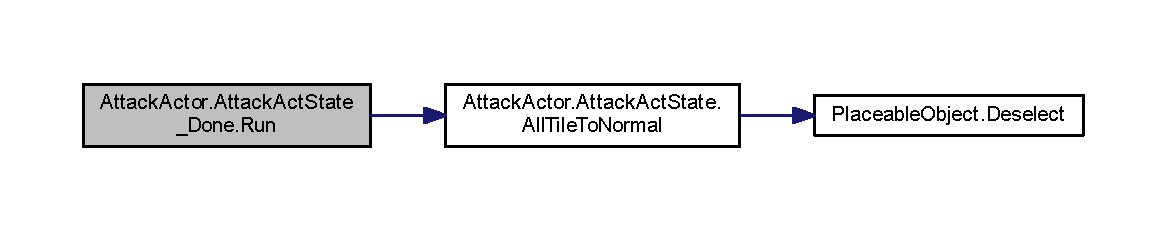
\includegraphics[width=350pt]{class_attack_actor_1_1_attack_act_state___done_a87dc9fe06b7132e7eff68fce885c2cd2_cgraph}
\end{center}
\end{figure}




\subsection{속성 문서화}
\index{Attack\+Actor\+::\+Attack\+Act\+State\+\_\+\+Done@{Attack\+Actor\+::\+Attack\+Act\+State\+\_\+\+Done}!Target@{Target}}
\index{Target@{Target}!Attack\+Actor\+::\+Attack\+Act\+State\+\_\+\+Done@{Attack\+Actor\+::\+Attack\+Act\+State\+\_\+\+Done}}
\subsubsection[{\texorpdfstring{Target}{Target}}]{\setlength{\rightskip}{0pt plus 5cm}T {\bf M\+C\+N.\+State}$<$ T $>$.Target\hspace{0.3cm}{\ttfamily [get]}, {\ttfamily [protected]}, {\ttfamily [inherited]}}\hypertarget{class_m_c_n_1_1_state_a93ba2fd920292031bd6e65b1dc505cb3}{}\label{class_m_c_n_1_1_state_a93ba2fd920292031bd6e65b1dc505cb3}


State.\+cs 파일의 32 번째 라인에서 정의되었습니다.



이 클래스에 대한 문서화 페이지는 다음의 파일로부터 생성되었습니다.\+:\begin{DoxyCompactItemize}
\item 
D\+:/\+Git\+Hub/\+M\+C\+N\+Tactics/\+Assets/\+Scripts/\+Objects/\+Actor/\hyperlink{_attack_actor_8cs}{Attack\+Actor.\+cs}\end{DoxyCompactItemize}

\hypertarget{class_attack_actor_1_1_attack_act_state___normal}{}\section{Attack\+Actor.\+Attack\+Act\+State\+\_\+\+Normal 클래스 참조}
\label{class_attack_actor_1_1_attack_act_state___normal}\index{Attack\+Actor.\+Attack\+Act\+State\+\_\+\+Normal@{Attack\+Actor.\+Attack\+Act\+State\+\_\+\+Normal}}


Attack\+Actor.\+Attack\+Act\+State\+\_\+\+Normal에 대한 상속 다이어그램 \+: 
\nopagebreak
\begin{figure}[H]
\begin{center}
\leavevmode
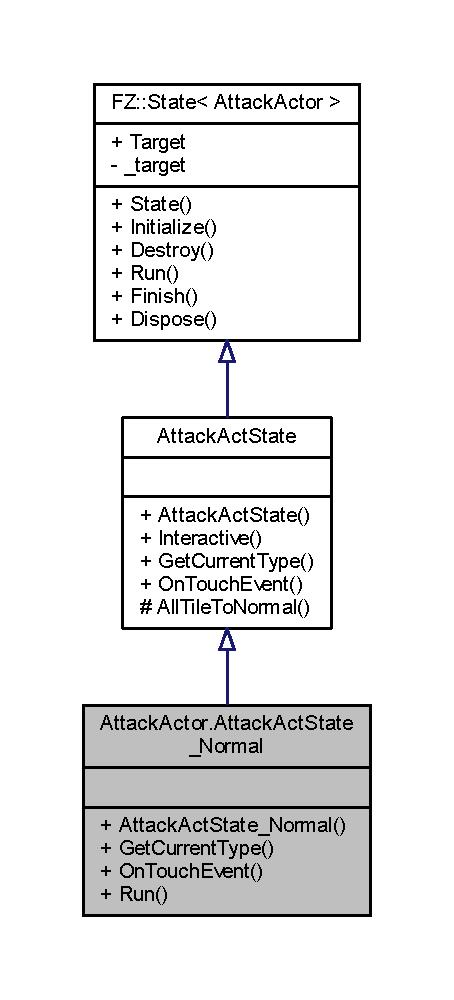
\includegraphics[width=218pt]{class_attack_actor_1_1_attack_act_state___normal__inherit__graph}
\end{center}
\end{figure}


Attack\+Actor.\+Attack\+Act\+State\+\_\+\+Normal에 대한 협력 다이어그램\+:
\nopagebreak
\begin{figure}[H]
\begin{center}
\leavevmode
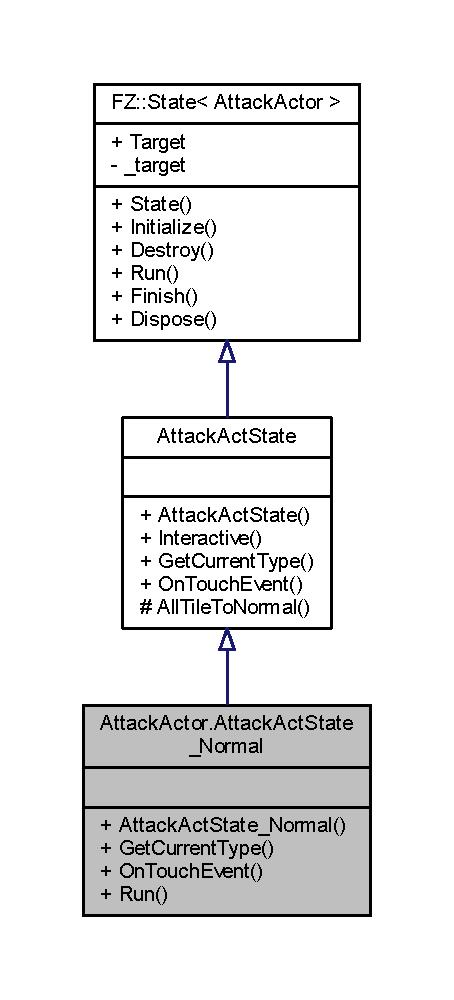
\includegraphics[width=218pt]{class_attack_actor_1_1_attack_act_state___normal__coll__graph}
\end{center}
\end{figure}
\subsection*{Public 멤버 함수}
\begin{DoxyCompactItemize}
\item 
\hyperlink{class_attack_actor_1_1_attack_act_state___normal_ab68b0ac3deec2c36e132dd8d635eef94}{Attack\+Act\+State\+\_\+\+Normal} (\hyperlink{class_attack_actor}{Attack\+Actor} target)
\item 
override \hyperlink{_attack_actor_8cs_a10659ce944335df4ded984f6bc41f31b}{e\+Attack\+Act\+Type} \hyperlink{class_attack_actor_1_1_attack_act_state___normal_a82484dc7be509e6a7a761c3c2b24a64a}{Get\+Current\+Type} ()
\item 
override bool \hyperlink{class_attack_actor_1_1_attack_act_state___normal_ac68685fce5e63f5b1d5fc3e8e74a5621}{On\+Touch\+Event} ()
\item 
override void \hyperlink{class_attack_actor_1_1_attack_act_state___normal_a7d6644fed269325b8f62138d8adb50f5}{Run} ()
\item 
virtual void \hyperlink{class_attack_actor_1_1_attack_act_state_a2ae9dd2f7ec8db76d25d7ad7ed58b89d}{Interactive} (\hyperlink{class_tile}{Tile} active\+Tile)
\item 
virtual void \hyperlink{class_m_c_n_1_1_state_a8eabaffe047e6dccd5c5d8aed7bf218a}{Initialize} ()
\item 
virtual void \hyperlink{class_m_c_n_1_1_state_a32af22a6a0a979d3b3a80225426aa839}{Destroy} ()
\item 
virtual void \hyperlink{class_m_c_n_1_1_state_a6de4f94b23916fcd05f589759da9ac3f}{Finish} ()
\item 
void \hyperlink{class_m_c_n_1_1_state_a6c53b2eda47e718ff469fd76a95cf02a}{Dispose} ()
\end{DoxyCompactItemize}
\subsection*{Protected 멤버 함수}
\begin{DoxyCompactItemize}
\item 
void \hyperlink{class_attack_actor_1_1_attack_act_state_a993762ec959af926e416f03fa7b71203}{All\+Tile\+To\+Normal} ()
\end{DoxyCompactItemize}
\subsection*{속성}
\begin{DoxyCompactItemize}
\item 
T \hyperlink{class_m_c_n_1_1_state_a93ba2fd920292031bd6e65b1dc505cb3}{Target}\hspace{0.3cm}{\ttfamily  \mbox{[}get\mbox{]}}
\end{DoxyCompactItemize}


\subsection{상세한 설명}


Attack\+Actor.\+cs 파일의 79 번째 라인에서 정의되었습니다.



\subsection{생성자 \& 소멸자 문서화}
\index{Attack\+Actor\+::\+Attack\+Act\+State\+\_\+\+Normal@{Attack\+Actor\+::\+Attack\+Act\+State\+\_\+\+Normal}!Attack\+Act\+State\+\_\+\+Normal@{Attack\+Act\+State\+\_\+\+Normal}}
\index{Attack\+Act\+State\+\_\+\+Normal@{Attack\+Act\+State\+\_\+\+Normal}!Attack\+Actor\+::\+Attack\+Act\+State\+\_\+\+Normal@{Attack\+Actor\+::\+Attack\+Act\+State\+\_\+\+Normal}}
\subsubsection[{\texorpdfstring{Attack\+Act\+State\+\_\+\+Normal(\+Attack\+Actor target)}{AttackActState_Normal(AttackActor target)}}]{\setlength{\rightskip}{0pt plus 5cm}Attack\+Actor.\+Attack\+Act\+State\+\_\+\+Normal.\+Attack\+Act\+State\+\_\+\+Normal (
\begin{DoxyParamCaption}
\item[{{\bf Attack\+Actor}}]{target}
\end{DoxyParamCaption}
)}\hypertarget{class_attack_actor_1_1_attack_act_state___normal_ab68b0ac3deec2c36e132dd8d635eef94}{}\label{class_attack_actor_1_1_attack_act_state___normal_ab68b0ac3deec2c36e132dd8d635eef94}


Attack\+Actor.\+cs 파일의 81 번째 라인에서 정의되었습니다.


\begin{DoxyCode}
81 : base(target) \{ \}
\end{DoxyCode}


\subsection{멤버 함수 문서화}
\index{Attack\+Actor\+::\+Attack\+Act\+State\+\_\+\+Normal@{Attack\+Actor\+::\+Attack\+Act\+State\+\_\+\+Normal}!All\+Tile\+To\+Normal@{All\+Tile\+To\+Normal}}
\index{All\+Tile\+To\+Normal@{All\+Tile\+To\+Normal}!Attack\+Actor\+::\+Attack\+Act\+State\+\_\+\+Normal@{Attack\+Actor\+::\+Attack\+Act\+State\+\_\+\+Normal}}
\subsubsection[{\texorpdfstring{All\+Tile\+To\+Normal()}{AllTileToNormal()}}]{\setlength{\rightskip}{0pt plus 5cm}void Attack\+Actor.\+Attack\+Act\+State.\+All\+Tile\+To\+Normal (
\begin{DoxyParamCaption}
{}
\end{DoxyParamCaption}
)\hspace{0.3cm}{\ttfamily [protected]}, {\ttfamily [inherited]}}\hypertarget{class_attack_actor_1_1_attack_act_state_a993762ec959af926e416f03fa7b71203}{}\label{class_attack_actor_1_1_attack_act_state_a993762ec959af926e416f03fa7b71203}


Attack\+Actor.\+cs 파일의 63 번째 라인에서 정의되었습니다.


\begin{DoxyCode}
64         \{
65             \textcolor{keywordflow}{if} (\hyperlink{class_m_c_n_1_1_state_a93ba2fd920292031bd6e65b1dc505cb3}{Target} != null)
66             \{
67                 var placeable = \hyperlink{class_m_c_n_1_1_state_a93ba2fd920292031bd6e65b1dc505cb3}{Target}.ActTarget as \hyperlink{class_placeable_object}{PlaceableObject};
68 
69                 \textcolor{keywordflow}{if} (placeable != null)
70                 \{
71                     placeable.\hyperlink{class_placeable_object_a0c1248b1f9981ddbf68e6f70a6498f3d}{Deselect}();
72 
73                     \hyperlink{class_map_manager}{MapManager}.\hyperlink{class_m_c_n_1_1_mono_singletone_aa50c027cca64cf4ad30c1ee5c83e0b78}{Instance}.ChangeAllTileState(
      \hyperlink{_tile_8cs_a271bc07be325bca511bcb747e0ff2fda}{eTileType}.NORMAL);
74                 \}
75             \}
76         \}
\end{DoxyCode}


이 함수 내부에서 호출하는 함수들에 대한 그래프입니다.\+:
\nopagebreak
\begin{figure}[H]
\begin{center}
\leavevmode
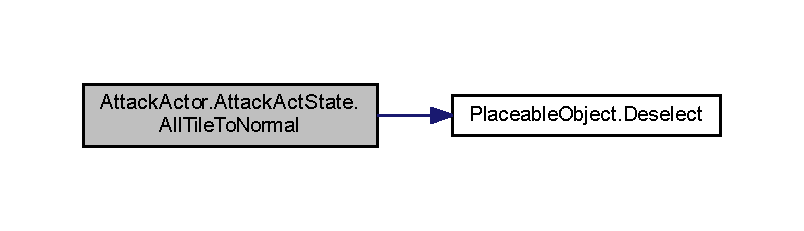
\includegraphics[width=350pt]{class_attack_actor_1_1_attack_act_state_a993762ec959af926e416f03fa7b71203_cgraph}
\end{center}
\end{figure}




이 함수를 호출하는 함수들에 대한 그래프입니다.\+:
\nopagebreak
\begin{figure}[H]
\begin{center}
\leavevmode
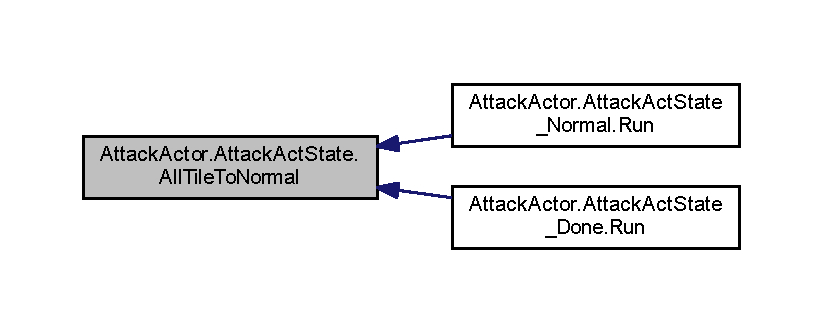
\includegraphics[width=350pt]{class_attack_actor_1_1_attack_act_state_a993762ec959af926e416f03fa7b71203_icgraph}
\end{center}
\end{figure}


\index{Attack\+Actor\+::\+Attack\+Act\+State\+\_\+\+Normal@{Attack\+Actor\+::\+Attack\+Act\+State\+\_\+\+Normal}!Destroy@{Destroy}}
\index{Destroy@{Destroy}!Attack\+Actor\+::\+Attack\+Act\+State\+\_\+\+Normal@{Attack\+Actor\+::\+Attack\+Act\+State\+\_\+\+Normal}}
\subsubsection[{\texorpdfstring{Destroy()}{Destroy()}}]{\setlength{\rightskip}{0pt plus 5cm}virtual void {\bf M\+C\+N.\+State}$<$ T $>$.Destroy (
\begin{DoxyParamCaption}
{}
\end{DoxyParamCaption}
)\hspace{0.3cm}{\ttfamily [virtual]}, {\ttfamily [inherited]}}\hypertarget{class_m_c_n_1_1_state_a32af22a6a0a979d3b3a80225426aa839}{}\label{class_m_c_n_1_1_state_a32af22a6a0a979d3b3a80225426aa839}


State.\+cs 파일의 47 번째 라인에서 정의되었습니다.


\begin{DoxyCode}
47 \{ \}
\end{DoxyCode}
\index{Attack\+Actor\+::\+Attack\+Act\+State\+\_\+\+Normal@{Attack\+Actor\+::\+Attack\+Act\+State\+\_\+\+Normal}!Dispose@{Dispose}}
\index{Dispose@{Dispose}!Attack\+Actor\+::\+Attack\+Act\+State\+\_\+\+Normal@{Attack\+Actor\+::\+Attack\+Act\+State\+\_\+\+Normal}}
\subsubsection[{\texorpdfstring{Dispose()}{Dispose()}}]{\setlength{\rightskip}{0pt plus 5cm}void {\bf M\+C\+N.\+State}$<$ T $>$.Dispose (
\begin{DoxyParamCaption}
{}
\end{DoxyParamCaption}
)\hspace{0.3cm}{\ttfamily [inherited]}}\hypertarget{class_m_c_n_1_1_state_a6c53b2eda47e718ff469fd76a95cf02a}{}\label{class_m_c_n_1_1_state_a6c53b2eda47e718ff469fd76a95cf02a}


State.\+cs 파일의 52 번째 라인에서 정의되었습니다.


\begin{DoxyCode}
53         \{
54             \hyperlink{class_m_c_n_1_1_state_ab759357c7d076cf62dd0016b743d762e}{\_target} = \textcolor{keywordflow}{default}(T);
55         \}
\end{DoxyCode}
\index{Attack\+Actor\+::\+Attack\+Act\+State\+\_\+\+Normal@{Attack\+Actor\+::\+Attack\+Act\+State\+\_\+\+Normal}!Finish@{Finish}}
\index{Finish@{Finish}!Attack\+Actor\+::\+Attack\+Act\+State\+\_\+\+Normal@{Attack\+Actor\+::\+Attack\+Act\+State\+\_\+\+Normal}}
\subsubsection[{\texorpdfstring{Finish()}{Finish()}}]{\setlength{\rightskip}{0pt plus 5cm}virtual void {\bf M\+C\+N.\+State}$<$ T $>$.Finish (
\begin{DoxyParamCaption}
{}
\end{DoxyParamCaption}
)\hspace{0.3cm}{\ttfamily [virtual]}, {\ttfamily [inherited]}}\hypertarget{class_m_c_n_1_1_state_a6de4f94b23916fcd05f589759da9ac3f}{}\label{class_m_c_n_1_1_state_a6de4f94b23916fcd05f589759da9ac3f}


State.\+cs 파일의 50 번째 라인에서 정의되었습니다.


\begin{DoxyCode}
50 \{ \}
\end{DoxyCode}
\index{Attack\+Actor\+::\+Attack\+Act\+State\+\_\+\+Normal@{Attack\+Actor\+::\+Attack\+Act\+State\+\_\+\+Normal}!Get\+Current\+Type@{Get\+Current\+Type}}
\index{Get\+Current\+Type@{Get\+Current\+Type}!Attack\+Actor\+::\+Attack\+Act\+State\+\_\+\+Normal@{Attack\+Actor\+::\+Attack\+Act\+State\+\_\+\+Normal}}
\subsubsection[{\texorpdfstring{Get\+Current\+Type()}{GetCurrentType()}}]{\setlength{\rightskip}{0pt plus 5cm}override {\bf e\+Attack\+Act\+Type} Attack\+Actor.\+Attack\+Act\+State\+\_\+\+Normal.\+Get\+Current\+Type (
\begin{DoxyParamCaption}
{}
\end{DoxyParamCaption}
)\hspace{0.3cm}{\ttfamily [virtual]}}\hypertarget{class_attack_actor_1_1_attack_act_state___normal_a82484dc7be509e6a7a761c3c2b24a64a}{}\label{class_attack_actor_1_1_attack_act_state___normal_a82484dc7be509e6a7a761c3c2b24a64a}


\hyperlink{class_attack_actor_1_1_attack_act_state_a8657ce92996ace441bb68b9e3002aa56}{Attack\+Actor.\+Attack\+Act\+State}를 구현.



Attack\+Actor.\+cs 파일의 83 번째 라인에서 정의되었습니다.


\begin{DoxyCode}
84         \{
85             \textcolor{keywordflow}{return} \hyperlink{_attack_actor_8cs_a10659ce944335df4ded984f6bc41f31b}{eAttackActType}.NORMAL;
86         \}
\end{DoxyCode}
\index{Attack\+Actor\+::\+Attack\+Act\+State\+\_\+\+Normal@{Attack\+Actor\+::\+Attack\+Act\+State\+\_\+\+Normal}!Initialize@{Initialize}}
\index{Initialize@{Initialize}!Attack\+Actor\+::\+Attack\+Act\+State\+\_\+\+Normal@{Attack\+Actor\+::\+Attack\+Act\+State\+\_\+\+Normal}}
\subsubsection[{\texorpdfstring{Initialize()}{Initialize()}}]{\setlength{\rightskip}{0pt plus 5cm}virtual void {\bf M\+C\+N.\+State}$<$ T $>$.Initialize (
\begin{DoxyParamCaption}
{}
\end{DoxyParamCaption}
)\hspace{0.3cm}{\ttfamily [virtual]}, {\ttfamily [inherited]}}\hypertarget{class_m_c_n_1_1_state_a8eabaffe047e6dccd5c5d8aed7bf218a}{}\label{class_m_c_n_1_1_state_a8eabaffe047e6dccd5c5d8aed7bf218a}


State.\+cs 파일의 46 번째 라인에서 정의되었습니다.


\begin{DoxyCode}
46 \{ \}
\end{DoxyCode}
\index{Attack\+Actor\+::\+Attack\+Act\+State\+\_\+\+Normal@{Attack\+Actor\+::\+Attack\+Act\+State\+\_\+\+Normal}!Interactive@{Interactive}}
\index{Interactive@{Interactive}!Attack\+Actor\+::\+Attack\+Act\+State\+\_\+\+Normal@{Attack\+Actor\+::\+Attack\+Act\+State\+\_\+\+Normal}}
\subsubsection[{\texorpdfstring{Interactive(\+Tile active\+Tile)}{Interactive(Tile activeTile)}}]{\setlength{\rightskip}{0pt plus 5cm}virtual void Attack\+Actor.\+Attack\+Act\+State.\+Interactive (
\begin{DoxyParamCaption}
\item[{{\bf Tile}}]{active\+Tile}
\end{DoxyParamCaption}
)\hspace{0.3cm}{\ttfamily [virtual]}, {\ttfamily [inherited]}}\hypertarget{class_attack_actor_1_1_attack_act_state_a2ae9dd2f7ec8db76d25d7ad7ed58b89d}{}\label{class_attack_actor_1_1_attack_act_state_a2ae9dd2f7ec8db76d25d7ad7ed58b89d}


\hyperlink{class_attack_actor_1_1_attack_act_state___attack_a59a3f2e994baeddabb870446b5df1641}{Attack\+Actor.\+Attack\+Act\+State\+\_\+\+Attack}에서 재구현되었습니다.



Attack\+Actor.\+cs 파일의 57 번째 라인에서 정의되었습니다.


\begin{DoxyCode}
57 \{ \}
\end{DoxyCode}


이 함수 내부에서 호출하는 함수들에 대한 그래프입니다.\+:
\nopagebreak
\begin{figure}[H]
\begin{center}
\leavevmode
\includegraphics[width=350pt]{class_attack_actor_1_1_attack_act_state_a2ae9dd2f7ec8db76d25d7ad7ed58b89d_cgraph}
\end{center}
\end{figure}


\index{Attack\+Actor\+::\+Attack\+Act\+State\+\_\+\+Normal@{Attack\+Actor\+::\+Attack\+Act\+State\+\_\+\+Normal}!On\+Touch\+Event@{On\+Touch\+Event}}
\index{On\+Touch\+Event@{On\+Touch\+Event}!Attack\+Actor\+::\+Attack\+Act\+State\+\_\+\+Normal@{Attack\+Actor\+::\+Attack\+Act\+State\+\_\+\+Normal}}
\subsubsection[{\texorpdfstring{On\+Touch\+Event()}{OnTouchEvent()}}]{\setlength{\rightskip}{0pt plus 5cm}override bool Attack\+Actor.\+Attack\+Act\+State\+\_\+\+Normal.\+On\+Touch\+Event (
\begin{DoxyParamCaption}
{}
\end{DoxyParamCaption}
)\hspace{0.3cm}{\ttfamily [virtual]}}\hypertarget{class_attack_actor_1_1_attack_act_state___normal_ac68685fce5e63f5b1d5fc3e8e74a5621}{}\label{class_attack_actor_1_1_attack_act_state___normal_ac68685fce5e63f5b1d5fc3e8e74a5621}


\hyperlink{class_attack_actor_1_1_attack_act_state_aa5e1794a3ede54c3b71a1463bf5b79a4}{Attack\+Actor.\+Attack\+Act\+State}를 구현.



Attack\+Actor.\+cs 파일의 88 번째 라인에서 정의되었습니다.


\begin{DoxyCode}
89         \{
90             \textcolor{keywordflow}{if} (\hyperlink{class_m_c_n_1_1_state_a93ba2fd920292031bd6e65b1dc505cb3}{Target} != null)
91             \{
92                 \textcolor{keywordflow}{if} (\hyperlink{class_m_c_n_1_1_state_a93ba2fd920292031bd6e65b1dc505cb3}{Target}.GetCurrentStateType() != \hyperlink{_attack_actor_8cs_a10659ce944335df4ded984f6bc41f31b}{eAttackActType}.DONE)
93                 \{
94                     \textcolor{keywordflow}{if} (\hyperlink{class_game_manager}{GameManager}.\hyperlink{class_m_c_n_1_1_singletone_a46dbbebd93e96a9592a9803c51f35602}{Instance}.SelectedObj == null)
95                     \{
96                         \hyperlink{class_m_c_n_1_1_state_a93ba2fd920292031bd6e65b1dc505cb3}{Target}.ChangeState(\hyperlink{_attack_actor_8cs_a10659ce944335df4ded984f6bc41f31b}{eAttackActType}.ATTACK);
97                     \}
98                 \}
99             \}
100 
101             \textcolor{keywordflow}{return} \textcolor{keyword}{false};
102         \}
\end{DoxyCode}
\index{Attack\+Actor\+::\+Attack\+Act\+State\+\_\+\+Normal@{Attack\+Actor\+::\+Attack\+Act\+State\+\_\+\+Normal}!Run@{Run}}
\index{Run@{Run}!Attack\+Actor\+::\+Attack\+Act\+State\+\_\+\+Normal@{Attack\+Actor\+::\+Attack\+Act\+State\+\_\+\+Normal}}
\subsubsection[{\texorpdfstring{Run()}{Run()}}]{\setlength{\rightskip}{0pt plus 5cm}override void Attack\+Actor.\+Attack\+Act\+State\+\_\+\+Normal.\+Run (
\begin{DoxyParamCaption}
{}
\end{DoxyParamCaption}
)\hspace{0.3cm}{\ttfamily [virtual]}}\hypertarget{class_attack_actor_1_1_attack_act_state___normal_a7d6644fed269325b8f62138d8adb50f5}{}\label{class_attack_actor_1_1_attack_act_state___normal_a7d6644fed269325b8f62138d8adb50f5}


\hyperlink{class_m_c_n_1_1_state_a8adfea67c55997e5c0eefbae1e429f4d}{M\+C\+N.\+State$<$ Attack\+Actor $>$}를 구현.



Attack\+Actor.\+cs 파일의 104 번째 라인에서 정의되었습니다.


\begin{DoxyCode}
105         \{
106             \hyperlink{class_attack_actor_1_1_attack_act_state_a993762ec959af926e416f03fa7b71203}{AllTileToNormal}();
107         \}
\end{DoxyCode}


이 함수 내부에서 호출하는 함수들에 대한 그래프입니다.\+:
\nopagebreak
\begin{figure}[H]
\begin{center}
\leavevmode
\includegraphics[width=350pt]{class_attack_actor_1_1_attack_act_state___normal_a7d6644fed269325b8f62138d8adb50f5_cgraph}
\end{center}
\end{figure}




\subsection{속성 문서화}
\index{Attack\+Actor\+::\+Attack\+Act\+State\+\_\+\+Normal@{Attack\+Actor\+::\+Attack\+Act\+State\+\_\+\+Normal}!Target@{Target}}
\index{Target@{Target}!Attack\+Actor\+::\+Attack\+Act\+State\+\_\+\+Normal@{Attack\+Actor\+::\+Attack\+Act\+State\+\_\+\+Normal}}
\subsubsection[{\texorpdfstring{Target}{Target}}]{\setlength{\rightskip}{0pt plus 5cm}T {\bf M\+C\+N.\+State}$<$ T $>$.Target\hspace{0.3cm}{\ttfamily [get]}, {\ttfamily [protected]}, {\ttfamily [inherited]}}\hypertarget{class_m_c_n_1_1_state_a93ba2fd920292031bd6e65b1dc505cb3}{}\label{class_m_c_n_1_1_state_a93ba2fd920292031bd6e65b1dc505cb3}


State.\+cs 파일의 32 번째 라인에서 정의되었습니다.



이 클래스에 대한 문서화 페이지는 다음의 파일로부터 생성되었습니다.\+:\begin{DoxyCompactItemize}
\item 
D\+:/\+Git\+Hub/\+M\+C\+N\+Tactics/\+Assets/\+Scripts/\+Objects/\+Actor/\hyperlink{_attack_actor_8cs}{Attack\+Actor.\+cs}\end{DoxyCompactItemize}

\hypertarget{class_combat_added_deco}{}\section{Combat\+Added\+Deco 클래스 참조}
\label{class_combat_added_deco}\index{Combat\+Added\+Deco@{Combat\+Added\+Deco}}


Combat\+Added\+Deco에 대한 상속 다이어그램 \+: 
\nopagebreak
\begin{figure}[H]
\begin{center}
\leavevmode
\includegraphics[width=312pt]{class_combat_added_deco__inherit__graph}
\end{center}
\end{figure}


Combat\+Added\+Deco에 대한 협력 다이어그램\+:
\nopagebreak
\begin{figure}[H]
\begin{center}
\leavevmode
\includegraphics[width=312pt]{class_combat_added_deco__coll__graph}
\end{center}
\end{figure}
\subsection*{Public 멤버 함수}
\begin{DoxyCompactItemize}
\item 
\hyperlink{class_combat_added_deco_a18e349f5ae6041f6b2d1d1844b59987a}{Combat\+Added\+Deco} (\hyperlink{interface_i_combat}{I\+Combat} target, \hyperlink{struct_status}{Status} added\+Status)
\item 
void \hyperlink{class_combat_added_deco_a3f1bc69d50b10571339d651eaa093a43}{Damaged} (\hyperlink{class_attack_actor}{Attack\+Actor} actor)
\end{DoxyCompactItemize}
\subsection*{Protected 속성}
\begin{DoxyCompactItemize}
\item 
T \hyperlink{class_f_z_1_1_decorator_adce2c6d288dcfa08b899f3e233190210}{\+\_\+deco\+Target}
\end{DoxyCompactItemize}
\subsection*{속성}
\begin{DoxyCompactItemize}
\item 
int \hyperlink{class_combat_added_deco_aeb5992435525404a992ee9f028a2cf0d}{Atk}\hspace{0.3cm}{\ttfamily  \mbox{[}get\mbox{]}}
\item 
int \hyperlink{class_combat_added_deco_ac3d7d042df2e8c8cbec3d6cbcb85ae96}{Def}\hspace{0.3cm}{\ttfamily  \mbox{[}get\mbox{]}}
\item 
int \hyperlink{class_combat_added_deco_a6810b0a4d852d7f8dc61145e2c7c9fc4}{Hp}\hspace{0.3cm}{\ttfamily  \mbox{[}get\mbox{]}}
\item 
int \hyperlink{class_combat_added_deco_aac41784d0f685c5db6107affca78d089}{Sp}\hspace{0.3cm}{\ttfamily  \mbox{[}get\mbox{]}}
\item 
int \hyperlink{class_combat_added_deco_a6e24be83c5d6b04b0d900103bb398d2e}{Max\+Hp}\hspace{0.3cm}{\ttfamily  \mbox{[}get\mbox{]}}
\item 
int \hyperlink{class_combat_added_deco_aa1dde14484472ac5d8b42d3ee9b745f2}{Max\+Sp}\hspace{0.3cm}{\ttfamily  \mbox{[}get\mbox{]}}
\item 
\hyperlink{_unit_object_8cs_ae6d9f4a8ae9fffcdf1a546168a44f917}{e\+Combat\+State} \hyperlink{class_combat_added_deco_a16e7a3ae7dc8751d25ef0b6ee0ce5531}{Combat\+State}\hspace{0.3cm}{\ttfamily  \mbox{[}get\mbox{]}}
\end{DoxyCompactItemize}
\subsection*{Private 속성}
\begin{DoxyCompactItemize}
\item 
int \hyperlink{class_combat_added_deco_ae3e4d0cbbf900b51cadf756154b9cd80}{\+\_\+added\+Atk}
\item 
int \hyperlink{class_combat_added_deco_abb40c78d41f1f133a285415b70506940}{\+\_\+added\+Def}
\item 
int \hyperlink{class_combat_added_deco_aa6d7287956c39e242ed254faf29e6a3b}{\+\_\+added\+Hp}
\item 
int \hyperlink{class_combat_added_deco_a02d5c40dcf180b1ad7086856dfa83929}{\+\_\+added\+Sp}
\end{DoxyCompactItemize}


\subsection{상세한 설명}


Combat\+Added\+Deco.\+cs 파일의 3 번째 라인에서 정의되었습니다.



\subsection{생성자 \& 소멸자 문서화}
\index{Combat\+Added\+Deco@{Combat\+Added\+Deco}!Combat\+Added\+Deco@{Combat\+Added\+Deco}}
\index{Combat\+Added\+Deco@{Combat\+Added\+Deco}!Combat\+Added\+Deco@{Combat\+Added\+Deco}}
\subsubsection[{\texorpdfstring{Combat\+Added\+Deco(\+I\+Combat target, Status added\+Status)}{CombatAddedDeco(ICombat target, Status addedStatus)}}]{\setlength{\rightskip}{0pt plus 5cm}Combat\+Added\+Deco.\+Combat\+Added\+Deco (
\begin{DoxyParamCaption}
\item[{{\bf I\+Combat}}]{target, }
\item[{{\bf Status}}]{added\+Status}
\end{DoxyParamCaption}
)}\hypertarget{class_combat_added_deco_a18e349f5ae6041f6b2d1d1844b59987a}{}\label{class_combat_added_deco_a18e349f5ae6041f6b2d1d1844b59987a}


Combat\+Added\+Deco.\+cs 파일의 10 번째 라인에서 정의되었습니다.


\begin{DoxyCode}
10                                                                : base(target)
11     \{
12         this.\hyperlink{class_combat_added_deco_ae3e4d0cbbf900b51cadf756154b9cd80}{\_addedAtk} = addedStatus.\hyperlink{struct_status_a60abcd71f2c5226ae8466b01b1fa56e6}{Atk};
13         this.\hyperlink{class_combat_added_deco_abb40c78d41f1f133a285415b70506940}{\_addedDef} = addedStatus.\hyperlink{struct_status_a57d7e201d642441114f0426e449f6b45}{Def};
14         this.\hyperlink{class_combat_added_deco_aa6d7287956c39e242ed254faf29e6a3b}{\_addedHp} = addedStatus.\hyperlink{struct_status_a81b0c200ac8f8285e57cd4cc7bfd1fbf}{Hp};
15         this.\hyperlink{class_combat_added_deco_a02d5c40dcf180b1ad7086856dfa83929}{\_addedSp} = addedStatus.\hyperlink{struct_status_a71c109a2932f2f43a780485f6bf1209d}{Sp};
16     \}
\end{DoxyCode}


\subsection{멤버 함수 문서화}
\index{Combat\+Added\+Deco@{Combat\+Added\+Deco}!Damaged@{Damaged}}
\index{Damaged@{Damaged}!Combat\+Added\+Deco@{Combat\+Added\+Deco}}
\subsubsection[{\texorpdfstring{Damaged(\+Attack\+Actor actor)}{Damaged(AttackActor actor)}}]{\setlength{\rightskip}{0pt plus 5cm}void Combat\+Added\+Deco.\+Damaged (
\begin{DoxyParamCaption}
\item[{{\bf Attack\+Actor}}]{actor}
\end{DoxyParamCaption}
)}\hypertarget{class_combat_added_deco_a3f1bc69d50b10571339d651eaa093a43}{}\label{class_combat_added_deco_a3f1bc69d50b10571339d651eaa093a43}


\hyperlink{interface_i_combat_ab8df637ef6ddd1c4a0689cafba32f3b9}{I\+Combat}를 구현.



Combat\+Added\+Deco.\+cs 파일의 32 번째 라인에서 정의되었습니다.


\begin{DoxyCode}
33     \{
34         \hyperlink{class_f_z_1_1_decorator_adce2c6d288dcfa08b899f3e233190210}{\_decoTarget}.Damaged(actor);
35     \}
\end{DoxyCode}


\subsection{멤버 데이타 문서화}
\index{Combat\+Added\+Deco@{Combat\+Added\+Deco}!\+\_\+added\+Atk@{\+\_\+added\+Atk}}
\index{\+\_\+added\+Atk@{\+\_\+added\+Atk}!Combat\+Added\+Deco@{Combat\+Added\+Deco}}
\subsubsection[{\texorpdfstring{\+\_\+added\+Atk}{_addedAtk}}]{\setlength{\rightskip}{0pt plus 5cm}int Combat\+Added\+Deco.\+\_\+added\+Atk\hspace{0.3cm}{\ttfamily [private]}}\hypertarget{class_combat_added_deco_ae3e4d0cbbf900b51cadf756154b9cd80}{}\label{class_combat_added_deco_ae3e4d0cbbf900b51cadf756154b9cd80}


Combat\+Added\+Deco.\+cs 파일의 5 번째 라인에서 정의되었습니다.

\index{Combat\+Added\+Deco@{Combat\+Added\+Deco}!\+\_\+added\+Def@{\+\_\+added\+Def}}
\index{\+\_\+added\+Def@{\+\_\+added\+Def}!Combat\+Added\+Deco@{Combat\+Added\+Deco}}
\subsubsection[{\texorpdfstring{\+\_\+added\+Def}{_addedDef}}]{\setlength{\rightskip}{0pt plus 5cm}int Combat\+Added\+Deco.\+\_\+added\+Def\hspace{0.3cm}{\ttfamily [private]}}\hypertarget{class_combat_added_deco_abb40c78d41f1f133a285415b70506940}{}\label{class_combat_added_deco_abb40c78d41f1f133a285415b70506940}


Combat\+Added\+Deco.\+cs 파일의 6 번째 라인에서 정의되었습니다.

\index{Combat\+Added\+Deco@{Combat\+Added\+Deco}!\+\_\+added\+Hp@{\+\_\+added\+Hp}}
\index{\+\_\+added\+Hp@{\+\_\+added\+Hp}!Combat\+Added\+Deco@{Combat\+Added\+Deco}}
\subsubsection[{\texorpdfstring{\+\_\+added\+Hp}{_addedHp}}]{\setlength{\rightskip}{0pt plus 5cm}int Combat\+Added\+Deco.\+\_\+added\+Hp\hspace{0.3cm}{\ttfamily [private]}}\hypertarget{class_combat_added_deco_aa6d7287956c39e242ed254faf29e6a3b}{}\label{class_combat_added_deco_aa6d7287956c39e242ed254faf29e6a3b}


Combat\+Added\+Deco.\+cs 파일의 7 번째 라인에서 정의되었습니다.

\index{Combat\+Added\+Deco@{Combat\+Added\+Deco}!\+\_\+added\+Sp@{\+\_\+added\+Sp}}
\index{\+\_\+added\+Sp@{\+\_\+added\+Sp}!Combat\+Added\+Deco@{Combat\+Added\+Deco}}
\subsubsection[{\texorpdfstring{\+\_\+added\+Sp}{_addedSp}}]{\setlength{\rightskip}{0pt plus 5cm}int Combat\+Added\+Deco.\+\_\+added\+Sp\hspace{0.3cm}{\ttfamily [private]}}\hypertarget{class_combat_added_deco_a02d5c40dcf180b1ad7086856dfa83929}{}\label{class_combat_added_deco_a02d5c40dcf180b1ad7086856dfa83929}


Combat\+Added\+Deco.\+cs 파일의 8 번째 라인에서 정의되었습니다.

\index{Combat\+Added\+Deco@{Combat\+Added\+Deco}!\+\_\+deco\+Target@{\+\_\+deco\+Target}}
\index{\+\_\+deco\+Target@{\+\_\+deco\+Target}!Combat\+Added\+Deco@{Combat\+Added\+Deco}}
\subsubsection[{\texorpdfstring{\+\_\+deco\+Target}{_decoTarget}}]{\setlength{\rightskip}{0pt plus 5cm}T {\bf F\+Z.\+Decorator}$<$ T $>$.\+\_\+deco\+Target\hspace{0.3cm}{\ttfamily [protected]}, {\ttfamily [inherited]}}\hypertarget{class_f_z_1_1_decorator_adce2c6d288dcfa08b899f3e233190210}{}\label{class_f_z_1_1_decorator_adce2c6d288dcfa08b899f3e233190210}


Decorator.\+cs 파일의 9 번째 라인에서 정의되었습니다.



\subsection{속성 문서화}
\index{Combat\+Added\+Deco@{Combat\+Added\+Deco}!Atk@{Atk}}
\index{Atk@{Atk}!Combat\+Added\+Deco@{Combat\+Added\+Deco}}
\subsubsection[{\texorpdfstring{Atk}{Atk}}]{\setlength{\rightskip}{0pt plus 5cm}int Combat\+Added\+Deco.\+Atk\hspace{0.3cm}{\ttfamily [get]}}\hypertarget{class_combat_added_deco_aeb5992435525404a992ee9f028a2cf0d}{}\label{class_combat_added_deco_aeb5992435525404a992ee9f028a2cf0d}


Combat\+Added\+Deco.\+cs 파일의 18 번째 라인에서 정의되었습니다.

\index{Combat\+Added\+Deco@{Combat\+Added\+Deco}!Combat\+State@{Combat\+State}}
\index{Combat\+State@{Combat\+State}!Combat\+Added\+Deco@{Combat\+Added\+Deco}}
\subsubsection[{\texorpdfstring{Combat\+State}{CombatState}}]{\setlength{\rightskip}{0pt plus 5cm}{\bf e\+Combat\+State} Combat\+Added\+Deco.\+Combat\+State\hspace{0.3cm}{\ttfamily [get]}}\hypertarget{class_combat_added_deco_a16e7a3ae7dc8751d25ef0b6ee0ce5531}{}\label{class_combat_added_deco_a16e7a3ae7dc8751d25ef0b6ee0ce5531}


Combat\+Added\+Deco.\+cs 파일의 30 번째 라인에서 정의되었습니다.

\index{Combat\+Added\+Deco@{Combat\+Added\+Deco}!Def@{Def}}
\index{Def@{Def}!Combat\+Added\+Deco@{Combat\+Added\+Deco}}
\subsubsection[{\texorpdfstring{Def}{Def}}]{\setlength{\rightskip}{0pt plus 5cm}int Combat\+Added\+Deco.\+Def\hspace{0.3cm}{\ttfamily [get]}}\hypertarget{class_combat_added_deco_ac3d7d042df2e8c8cbec3d6cbcb85ae96}{}\label{class_combat_added_deco_ac3d7d042df2e8c8cbec3d6cbcb85ae96}


Combat\+Added\+Deco.\+cs 파일의 20 번째 라인에서 정의되었습니다.

\index{Combat\+Added\+Deco@{Combat\+Added\+Deco}!Hp@{Hp}}
\index{Hp@{Hp}!Combat\+Added\+Deco@{Combat\+Added\+Deco}}
\subsubsection[{\texorpdfstring{Hp}{Hp}}]{\setlength{\rightskip}{0pt plus 5cm}int Combat\+Added\+Deco.\+Hp\hspace{0.3cm}{\ttfamily [get]}}\hypertarget{class_combat_added_deco_a6810b0a4d852d7f8dc61145e2c7c9fc4}{}\label{class_combat_added_deco_a6810b0a4d852d7f8dc61145e2c7c9fc4}


Combat\+Added\+Deco.\+cs 파일의 22 번째 라인에서 정의되었습니다.

\index{Combat\+Added\+Deco@{Combat\+Added\+Deco}!Max\+Hp@{Max\+Hp}}
\index{Max\+Hp@{Max\+Hp}!Combat\+Added\+Deco@{Combat\+Added\+Deco}}
\subsubsection[{\texorpdfstring{Max\+Hp}{MaxHp}}]{\setlength{\rightskip}{0pt plus 5cm}int Combat\+Added\+Deco.\+Max\+Hp\hspace{0.3cm}{\ttfamily [get]}}\hypertarget{class_combat_added_deco_a6e24be83c5d6b04b0d900103bb398d2e}{}\label{class_combat_added_deco_a6e24be83c5d6b04b0d900103bb398d2e}


Combat\+Added\+Deco.\+cs 파일의 26 번째 라인에서 정의되었습니다.

\index{Combat\+Added\+Deco@{Combat\+Added\+Deco}!Max\+Sp@{Max\+Sp}}
\index{Max\+Sp@{Max\+Sp}!Combat\+Added\+Deco@{Combat\+Added\+Deco}}
\subsubsection[{\texorpdfstring{Max\+Sp}{MaxSp}}]{\setlength{\rightskip}{0pt plus 5cm}int Combat\+Added\+Deco.\+Max\+Sp\hspace{0.3cm}{\ttfamily [get]}}\hypertarget{class_combat_added_deco_aa1dde14484472ac5d8b42d3ee9b745f2}{}\label{class_combat_added_deco_aa1dde14484472ac5d8b42d3ee9b745f2}


Combat\+Added\+Deco.\+cs 파일의 28 번째 라인에서 정의되었습니다.

\index{Combat\+Added\+Deco@{Combat\+Added\+Deco}!Sp@{Sp}}
\index{Sp@{Sp}!Combat\+Added\+Deco@{Combat\+Added\+Deco}}
\subsubsection[{\texorpdfstring{Sp}{Sp}}]{\setlength{\rightskip}{0pt plus 5cm}int Combat\+Added\+Deco.\+Sp\hspace{0.3cm}{\ttfamily [get]}}\hypertarget{class_combat_added_deco_aac41784d0f685c5db6107affca78d089}{}\label{class_combat_added_deco_aac41784d0f685c5db6107affca78d089}


Combat\+Added\+Deco.\+cs 파일의 24 번째 라인에서 정의되었습니다.



이 클래스에 대한 문서화 페이지는 다음의 파일로부터 생성되었습니다.\+:\begin{DoxyCompactItemize}
\item 
D\+:/\+Git\+Hub/\+M\+C\+N\+Tactics/\+Assets/\+Scripts/\+Objects/\+Decorator/\hyperlink{_combat_added_deco_8cs}{Combat\+Added\+Deco.\+cs}\end{DoxyCompactItemize}

\hypertarget{class_combat_instance}{}\section{Combat\+Instance 클래스 참조}
\label{class_combat_instance}\index{Combat\+Instance@{Combat\+Instance}}


Combat\+Instance에 대한 상속 다이어그램 \+: 
\nopagebreak
\begin{figure}[H]
\begin{center}
\leavevmode
\includegraphics[width=182pt]{class_combat_instance__inherit__graph}
\end{center}
\end{figure}


Combat\+Instance에 대한 협력 다이어그램\+:
\nopagebreak
\begin{figure}[H]
\begin{center}
\leavevmode
\includegraphics[width=182pt]{class_combat_instance__coll__graph}
\end{center}
\end{figure}
\subsection*{Public 멤버 함수}
\begin{DoxyCompactItemize}
\item 
\hyperlink{class_combat_instance_a613a6f5a211954d3f5f0d621cab88606}{Combat\+Instance} (\hyperlink{struct_status}{Status} status)
\item 
void \hyperlink{class_combat_instance_a612a867750ddfc0da7306e73752225b7}{Damaged} (\hyperlink{class_attack_actor}{Attack\+Actor} actor)
\end{DoxyCompactItemize}
\subsection*{속성}
\begin{DoxyCompactItemize}
\item 
\hyperlink{_combat_object_8cs_ae6d9f4a8ae9fffcdf1a546168a44f917}{e\+Combat\+State} \hyperlink{class_combat_instance_a149d2068f3dc0ec72f3461d101dcebab}{Combat\+State}\hspace{0.3cm}{\ttfamily  \mbox{[}get\mbox{]}}
\item 
int \hyperlink{class_combat_instance_ae4682b727ea05a59141f747341877eb6}{Hp}\hspace{0.3cm}{\ttfamily  \mbox{[}get\mbox{]}}
\item 
int \hyperlink{class_combat_instance_a120995296719b1fb1fa4cc55721ddba4}{Sp}\hspace{0.3cm}{\ttfamily  \mbox{[}get\mbox{]}}
\item 
int \hyperlink{class_combat_instance_a9de7c50888b56d9854709d132e69baa9}{Atk}\hspace{0.3cm}{\ttfamily  \mbox{[}get\mbox{]}}
\item 
int \hyperlink{class_combat_instance_ab52acfd86a70be3647d2f092e6816190}{Def}\hspace{0.3cm}{\ttfamily  \mbox{[}get\mbox{]}}
\item 
int \hyperlink{class_combat_instance_a33c5218456253d1a5c457fe6364b10d7}{Max\+Hp}\hspace{0.3cm}{\ttfamily  \mbox{[}get\mbox{]}}
\item 
int \hyperlink{class_combat_instance_ad1d6d4d72223021bd0130b069437463d}{Max\+Sp}\hspace{0.3cm}{\ttfamily  \mbox{[}get\mbox{]}}
\end{DoxyCompactItemize}
\subsection*{Private 속성}
\begin{DoxyCompactItemize}
\item 
int \hyperlink{class_combat_instance_a392329b865aa88f2a579fcb7e7a0a99b}{\+\_\+hp}
\item 
int \hyperlink{class_combat_instance_a3a9ee2ea52b19b5150386b52396621f9}{\+\_\+sp}
\item 
int \hyperlink{class_combat_instance_afce9395cdf3a359fb6eb982c0bf7f063}{\+\_\+max\+Hp}
\item 
int \hyperlink{class_combat_instance_a2489b1182b81f028cfd45f26fb2a7af0}{\+\_\+max\+Sp}
\item 
int \hyperlink{class_combat_instance_a7107dad81ca2638ed2ad30de391029e6}{\+\_\+atk}
\item 
int \hyperlink{class_combat_instance_a1c2bc3e91c7e2fee8b5d5f489eaa3d40}{\+\_\+def}
\item 
\hyperlink{_combat_object_8cs_ae6d9f4a8ae9fffcdf1a546168a44f917}{e\+Combat\+State} \hyperlink{class_combat_instance_a6352b66ef39484c9d76b03df56d26ee4}{\+\_\+combat\+State}
\end{DoxyCompactItemize}


\subsection{상세한 설명}


Combat\+Instance.\+cs 파일의 4 번째 라인에서 정의되었습니다.



\subsection{생성자 \& 소멸자 문서화}
\index{Combat\+Instance@{Combat\+Instance}!Combat\+Instance@{Combat\+Instance}}
\index{Combat\+Instance@{Combat\+Instance}!Combat\+Instance@{Combat\+Instance}}
\subsubsection[{\texorpdfstring{Combat\+Instance(\+Status status)}{CombatInstance(Status status)}}]{\setlength{\rightskip}{0pt plus 5cm}Combat\+Instance.\+Combat\+Instance (
\begin{DoxyParamCaption}
\item[{{\bf Status}}]{status}
\end{DoxyParamCaption}
)}\hypertarget{class_combat_instance_a613a6f5a211954d3f5f0d621cab88606}{}\label{class_combat_instance_a613a6f5a211954d3f5f0d621cab88606}


Combat\+Instance.\+cs 파일의 38 번째 라인에서 정의되었습니다.


\begin{DoxyCode}
39     \{
40         \hyperlink{class_combat_instance_a6352b66ef39484c9d76b03df56d26ee4}{\_combatState} = \hyperlink{_combat_object_8cs_ae6d9f4a8ae9fffcdf1a546168a44f917}{eCombatState}.ALIVE;
41 
42         \hyperlink{class_combat_instance_a392329b865aa88f2a579fcb7e7a0a99b}{\_hp} = status.\hyperlink{struct_status_a6912591952ae3178114200d6383919df}{hp};
43         \hyperlink{class_combat_instance_a3a9ee2ea52b19b5150386b52396621f9}{\_sp} = status.\hyperlink{struct_status_a685aa4b12faa74a48a3b57f69e94084c}{sp};
44 
45         \hyperlink{class_combat_instance_afce9395cdf3a359fb6eb982c0bf7f063}{\_maxHp} = status.\hyperlink{struct_status_a6912591952ae3178114200d6383919df}{hp};
46         \hyperlink{class_combat_instance_a2489b1182b81f028cfd45f26fb2a7af0}{\_maxSp} = status.\hyperlink{struct_status_a685aa4b12faa74a48a3b57f69e94084c}{sp};
47 
48         \hyperlink{class_combat_instance_a7107dad81ca2638ed2ad30de391029e6}{\_atk} = status.\hyperlink{struct_status_aeaf2f82dd6fbce2adf2219b7a6b8227f}{atk};
49         \hyperlink{class_combat_instance_a1c2bc3e91c7e2fee8b5d5f489eaa3d40}{\_def} = status.\hyperlink{struct_status_a95a2f2a23ef79f2e0ced04621c4593c9}{def};
50     \}
\end{DoxyCode}


\subsection{멤버 함수 문서화}
\index{Combat\+Instance@{Combat\+Instance}!Damaged@{Damaged}}
\index{Damaged@{Damaged}!Combat\+Instance@{Combat\+Instance}}
\subsubsection[{\texorpdfstring{Damaged(\+Attack\+Actor actor)}{Damaged(AttackActor actor)}}]{\setlength{\rightskip}{0pt plus 5cm}void Combat\+Instance.\+Damaged (
\begin{DoxyParamCaption}
\item[{{\bf Attack\+Actor}}]{actor}
\end{DoxyParamCaption}
)}\hypertarget{class_combat_instance_a612a867750ddfc0da7306e73752225b7}{}\label{class_combat_instance_a612a867750ddfc0da7306e73752225b7}


\hyperlink{interface_i_combat_ab8df637ef6ddd1c4a0689cafba32f3b9}{I\+Combat}를 구현.



Combat\+Instance.\+cs 파일의 52 번째 라인에서 정의되었습니다.


\begin{DoxyCode}
53     \{
54         \hyperlink{class_combat_instance_a392329b865aa88f2a579fcb7e7a0a99b}{\_hp} -= actor.\hyperlink{class_attack_actor_aaa126531b12eeb6d03311d761697cc84}{Damage};
55 
56         \textcolor{keywordflow}{if}(\hyperlink{class_combat_instance_ae4682b727ea05a59141f747341877eb6}{Hp} < 0)
57         \{
58             \hyperlink{class_combat_instance_a6352b66ef39484c9d76b03df56d26ee4}{\_combatState} = \hyperlink{_combat_object_8cs_ae6d9f4a8ae9fffcdf1a546168a44f917}{eCombatState}.DEAD;
59         \}
60     \}
\end{DoxyCode}


\subsection{멤버 데이타 문서화}
\index{Combat\+Instance@{Combat\+Instance}!\+\_\+atk@{\+\_\+atk}}
\index{\+\_\+atk@{\+\_\+atk}!Combat\+Instance@{Combat\+Instance}}
\subsubsection[{\texorpdfstring{\+\_\+atk}{_atk}}]{\setlength{\rightskip}{0pt plus 5cm}int Combat\+Instance.\+\_\+atk\hspace{0.3cm}{\ttfamily [private]}}\hypertarget{class_combat_instance_a7107dad81ca2638ed2ad30de391029e6}{}\label{class_combat_instance_a7107dad81ca2638ed2ad30de391029e6}


Combat\+Instance.\+cs 파일의 12 번째 라인에서 정의되었습니다.

\index{Combat\+Instance@{Combat\+Instance}!\+\_\+combat\+State@{\+\_\+combat\+State}}
\index{\+\_\+combat\+State@{\+\_\+combat\+State}!Combat\+Instance@{Combat\+Instance}}
\subsubsection[{\texorpdfstring{\+\_\+combat\+State}{_combatState}}]{\setlength{\rightskip}{0pt plus 5cm}{\bf e\+Combat\+State} Combat\+Instance.\+\_\+combat\+State\hspace{0.3cm}{\ttfamily [private]}}\hypertarget{class_combat_instance_a6352b66ef39484c9d76b03df56d26ee4}{}\label{class_combat_instance_a6352b66ef39484c9d76b03df56d26ee4}


Combat\+Instance.\+cs 파일의 15 번째 라인에서 정의되었습니다.

\index{Combat\+Instance@{Combat\+Instance}!\+\_\+def@{\+\_\+def}}
\index{\+\_\+def@{\+\_\+def}!Combat\+Instance@{Combat\+Instance}}
\subsubsection[{\texorpdfstring{\+\_\+def}{_def}}]{\setlength{\rightskip}{0pt plus 5cm}int Combat\+Instance.\+\_\+def\hspace{0.3cm}{\ttfamily [private]}}\hypertarget{class_combat_instance_a1c2bc3e91c7e2fee8b5d5f489eaa3d40}{}\label{class_combat_instance_a1c2bc3e91c7e2fee8b5d5f489eaa3d40}


Combat\+Instance.\+cs 파일의 13 번째 라인에서 정의되었습니다.

\index{Combat\+Instance@{Combat\+Instance}!\+\_\+hp@{\+\_\+hp}}
\index{\+\_\+hp@{\+\_\+hp}!Combat\+Instance@{Combat\+Instance}}
\subsubsection[{\texorpdfstring{\+\_\+hp}{_hp}}]{\setlength{\rightskip}{0pt plus 5cm}int Combat\+Instance.\+\_\+hp\hspace{0.3cm}{\ttfamily [private]}}\hypertarget{class_combat_instance_a392329b865aa88f2a579fcb7e7a0a99b}{}\label{class_combat_instance_a392329b865aa88f2a579fcb7e7a0a99b}


Combat\+Instance.\+cs 파일의 6 번째 라인에서 정의되었습니다.

\index{Combat\+Instance@{Combat\+Instance}!\+\_\+max\+Hp@{\+\_\+max\+Hp}}
\index{\+\_\+max\+Hp@{\+\_\+max\+Hp}!Combat\+Instance@{Combat\+Instance}}
\subsubsection[{\texorpdfstring{\+\_\+max\+Hp}{_maxHp}}]{\setlength{\rightskip}{0pt plus 5cm}int Combat\+Instance.\+\_\+max\+Hp\hspace{0.3cm}{\ttfamily [private]}}\hypertarget{class_combat_instance_afce9395cdf3a359fb6eb982c0bf7f063}{}\label{class_combat_instance_afce9395cdf3a359fb6eb982c0bf7f063}


Combat\+Instance.\+cs 파일의 9 번째 라인에서 정의되었습니다.

\index{Combat\+Instance@{Combat\+Instance}!\+\_\+max\+Sp@{\+\_\+max\+Sp}}
\index{\+\_\+max\+Sp@{\+\_\+max\+Sp}!Combat\+Instance@{Combat\+Instance}}
\subsubsection[{\texorpdfstring{\+\_\+max\+Sp}{_maxSp}}]{\setlength{\rightskip}{0pt plus 5cm}int Combat\+Instance.\+\_\+max\+Sp\hspace{0.3cm}{\ttfamily [private]}}\hypertarget{class_combat_instance_a2489b1182b81f028cfd45f26fb2a7af0}{}\label{class_combat_instance_a2489b1182b81f028cfd45f26fb2a7af0}


Combat\+Instance.\+cs 파일의 10 번째 라인에서 정의되었습니다.

\index{Combat\+Instance@{Combat\+Instance}!\+\_\+sp@{\+\_\+sp}}
\index{\+\_\+sp@{\+\_\+sp}!Combat\+Instance@{Combat\+Instance}}
\subsubsection[{\texorpdfstring{\+\_\+sp}{_sp}}]{\setlength{\rightskip}{0pt plus 5cm}int Combat\+Instance.\+\_\+sp\hspace{0.3cm}{\ttfamily [private]}}\hypertarget{class_combat_instance_a3a9ee2ea52b19b5150386b52396621f9}{}\label{class_combat_instance_a3a9ee2ea52b19b5150386b52396621f9}


Combat\+Instance.\+cs 파일의 7 번째 라인에서 정의되었습니다.



\subsection{속성 문서화}
\index{Combat\+Instance@{Combat\+Instance}!Atk@{Atk}}
\index{Atk@{Atk}!Combat\+Instance@{Combat\+Instance}}
\subsubsection[{\texorpdfstring{Atk}{Atk}}]{\setlength{\rightskip}{0pt plus 5cm}int Combat\+Instance.\+Atk\hspace{0.3cm}{\ttfamily [get]}}\hypertarget{class_combat_instance_a9de7c50888b56d9854709d132e69baa9}{}\label{class_combat_instance_a9de7c50888b56d9854709d132e69baa9}


Combat\+Instance.\+cs 파일의 32 번째 라인에서 정의되었습니다.

\index{Combat\+Instance@{Combat\+Instance}!Combat\+State@{Combat\+State}}
\index{Combat\+State@{Combat\+State}!Combat\+Instance@{Combat\+Instance}}
\subsubsection[{\texorpdfstring{Combat\+State}{CombatState}}]{\setlength{\rightskip}{0pt plus 5cm}{\bf e\+Combat\+State} Combat\+Instance.\+Combat\+State\hspace{0.3cm}{\ttfamily [get]}}\hypertarget{class_combat_instance_a149d2068f3dc0ec72f3461d101dcebab}{}\label{class_combat_instance_a149d2068f3dc0ec72f3461d101dcebab}


Combat\+Instance.\+cs 파일의 16 번째 라인에서 정의되었습니다.

\index{Combat\+Instance@{Combat\+Instance}!Def@{Def}}
\index{Def@{Def}!Combat\+Instance@{Combat\+Instance}}
\subsubsection[{\texorpdfstring{Def}{Def}}]{\setlength{\rightskip}{0pt plus 5cm}int Combat\+Instance.\+Def\hspace{0.3cm}{\ttfamily [get]}}\hypertarget{class_combat_instance_ab52acfd86a70be3647d2f092e6816190}{}\label{class_combat_instance_ab52acfd86a70be3647d2f092e6816190}


Combat\+Instance.\+cs 파일의 33 번째 라인에서 정의되었습니다.

\index{Combat\+Instance@{Combat\+Instance}!Hp@{Hp}}
\index{Hp@{Hp}!Combat\+Instance@{Combat\+Instance}}
\subsubsection[{\texorpdfstring{Hp}{Hp}}]{\setlength{\rightskip}{0pt plus 5cm}int Combat\+Instance.\+Hp\hspace{0.3cm}{\ttfamily [get]}}\hypertarget{class_combat_instance_ae4682b727ea05a59141f747341877eb6}{}\label{class_combat_instance_ae4682b727ea05a59141f747341877eb6}


Combat\+Instance.\+cs 파일의 19 번째 라인에서 정의되었습니다.

\index{Combat\+Instance@{Combat\+Instance}!Max\+Hp@{Max\+Hp}}
\index{Max\+Hp@{Max\+Hp}!Combat\+Instance@{Combat\+Instance}}
\subsubsection[{\texorpdfstring{Max\+Hp}{MaxHp}}]{\setlength{\rightskip}{0pt plus 5cm}int Combat\+Instance.\+Max\+Hp\hspace{0.3cm}{\ttfamily [get]}}\hypertarget{class_combat_instance_a33c5218456253d1a5c457fe6364b10d7}{}\label{class_combat_instance_a33c5218456253d1a5c457fe6364b10d7}


Combat\+Instance.\+cs 파일의 35 번째 라인에서 정의되었습니다.

\index{Combat\+Instance@{Combat\+Instance}!Max\+Sp@{Max\+Sp}}
\index{Max\+Sp@{Max\+Sp}!Combat\+Instance@{Combat\+Instance}}
\subsubsection[{\texorpdfstring{Max\+Sp}{MaxSp}}]{\setlength{\rightskip}{0pt plus 5cm}int Combat\+Instance.\+Max\+Sp\hspace{0.3cm}{\ttfamily [get]}}\hypertarget{class_combat_instance_ad1d6d4d72223021bd0130b069437463d}{}\label{class_combat_instance_ad1d6d4d72223021bd0130b069437463d}


Combat\+Instance.\+cs 파일의 36 번째 라인에서 정의되었습니다.

\index{Combat\+Instance@{Combat\+Instance}!Sp@{Sp}}
\index{Sp@{Sp}!Combat\+Instance@{Combat\+Instance}}
\subsubsection[{\texorpdfstring{Sp}{Sp}}]{\setlength{\rightskip}{0pt plus 5cm}int Combat\+Instance.\+Sp\hspace{0.3cm}{\ttfamily [get]}}\hypertarget{class_combat_instance_a120995296719b1fb1fa4cc55721ddba4}{}\label{class_combat_instance_a120995296719b1fb1fa4cc55721ddba4}


Combat\+Instance.\+cs 파일의 30 번째 라인에서 정의되었습니다.



이 클래스에 대한 문서화 페이지는 다음의 파일로부터 생성되었습니다.\+:\begin{DoxyCompactItemize}
\item 
D\+:/\+Git\+Hub/\+M\+C\+N\+Tactics/\+Assets/\+Scripts/\+Objects/\+Decorator/\hyperlink{_combat_instance_8cs}{Combat\+Instance.\+cs}\end{DoxyCompactItemize}

\hypertarget{class_data_factory}{}\section{Data\+Factory 클래스 참조}
\label{class_data_factory}\index{Data\+Factory@{Data\+Factory}}


Data\+Factory에 대한 상속 다이어그램 \+: 
\nopagebreak
\begin{figure}[H]
\begin{center}
\leavevmode
\includegraphics[width=172pt]{class_data_factory__inherit__graph}
\end{center}
\end{figure}


Data\+Factory에 대한 협력 다이어그램\+:
\nopagebreak
\begin{figure}[H]
\begin{center}
\leavevmode
\includegraphics[width=172pt]{class_data_factory__coll__graph}
\end{center}
\end{figure}
\subsection*{클래스}
\begin{DoxyCompactItemize}
\item 
class \hyperlink{class_data_factory_1_1_json_parser}{Json\+Parser}
\end{DoxyCompactItemize}
\subsection*{Public 멤버 함수}
\begin{DoxyCompactItemize}
\item 
abstract \hyperlink{class_data_manager_ac9cb5bf021d3ebcc7f3eaa4bf5393408}{Data\+Manager.\+Data\+Type} \hyperlink{class_data_factory_a801f5669364ffcfd2a926022d5aef950}{Get\+Data\+Type} ()
\item 
abstract \hyperlink{class_data_object}{Data\+Object} \hyperlink{class_data_factory_a8ed29ae4a917c15aa824bb7f56418cbf}{Load\+Datas} ()
\end{DoxyCompactItemize}
\subsection*{Protected 멤버 함수}
\begin{DoxyCompactItemize}
\item 
abstract string \hyperlink{class_data_factory_af66cb0238bd7b6fc0b675ac48ced0eea}{Get\+Name} ()
\item 
string \hyperlink{class_data_factory_a5f040ba1715a670e29f45e07d22b4d5b}{Get\+Json\+String} ()
\end{DoxyCompactItemize}


\subsection{상세한 설명}


Data\+Manager.\+cs 파일의 42 번째 라인에서 정의되었습니다.



\subsection{멤버 함수 문서화}
\index{Data\+Factory@{Data\+Factory}!Get\+Data\+Type@{Get\+Data\+Type}}
\index{Get\+Data\+Type@{Get\+Data\+Type}!Data\+Factory@{Data\+Factory}}
\subsubsection[{\texorpdfstring{Get\+Data\+Type()}{GetDataType()}}]{\setlength{\rightskip}{0pt plus 5cm}abstract {\bf Data\+Manager.\+Data\+Type} Data\+Factory.\+Get\+Data\+Type (
\begin{DoxyParamCaption}
{}
\end{DoxyParamCaption}
)\hspace{0.3cm}{\ttfamily [pure virtual]}}\hypertarget{class_data_factory_a801f5669364ffcfd2a926022d5aef950}{}\label{class_data_factory_a801f5669364ffcfd2a926022d5aef950}


\hyperlink{class_unit_data_factory_af028480546af2388352b306060033720}{Unit\+Data\+Factory}에서 구현되었습니다.



이 함수를 호출하는 함수들에 대한 그래프입니다.\+:
\nopagebreak
\begin{figure}[H]
\begin{center}
\leavevmode
\includegraphics[width=350pt]{class_data_factory_a801f5669364ffcfd2a926022d5aef950_icgraph}
\end{center}
\end{figure}


\index{Data\+Factory@{Data\+Factory}!Get\+Json\+String@{Get\+Json\+String}}
\index{Get\+Json\+String@{Get\+Json\+String}!Data\+Factory@{Data\+Factory}}
\subsubsection[{\texorpdfstring{Get\+Json\+String()}{GetJsonString()}}]{\setlength{\rightskip}{0pt plus 5cm}string Data\+Factory.\+Get\+Json\+String (
\begin{DoxyParamCaption}
{}
\end{DoxyParamCaption}
)\hspace{0.3cm}{\ttfamily [protected]}}\hypertarget{class_data_factory_a5f040ba1715a670e29f45e07d22b4d5b}{}\label{class_data_factory_a5f040ba1715a670e29f45e07d22b4d5b}


Data\+Manager.\+cs 파일의 68 번째 라인에서 정의되었습니다.


\begin{DoxyCode}
69     \{
70         var textAsset = Resources.Load(\textcolor{keywordtype}{string}.Format(\textcolor{stringliteral}{"Data/\{0\}"}, \hyperlink{class_data_factory_af66cb0238bd7b6fc0b675ac48ced0eea}{GetName}())) as TextAsset;
71         \textcolor{keywordflow}{if} (textAsset != null)
72         \{
73             \textcolor{keywordflow}{return} textAsset.text;
74         \}
75         \textcolor{keywordflow}{else}
76         \{
77             \textcolor{keywordflow}{throw} \textcolor{keyword}{new} UnityException(\textcolor{stringliteral}{"DataFactory : DataPath is not available."});
78         \}
79     \}
\end{DoxyCode}


이 함수를 호출하는 함수들에 대한 그래프입니다.\+:
\nopagebreak
\begin{figure}[H]
\begin{center}
\leavevmode
\includegraphics[width=350pt]{class_data_factory_a5f040ba1715a670e29f45e07d22b4d5b_icgraph}
\end{center}
\end{figure}


\index{Data\+Factory@{Data\+Factory}!Get\+Name@{Get\+Name}}
\index{Get\+Name@{Get\+Name}!Data\+Factory@{Data\+Factory}}
\subsubsection[{\texorpdfstring{Get\+Name()}{GetName()}}]{\setlength{\rightskip}{0pt plus 5cm}abstract string Data\+Factory.\+Get\+Name (
\begin{DoxyParamCaption}
{}
\end{DoxyParamCaption}
)\hspace{0.3cm}{\ttfamily [protected]}, {\ttfamily [pure virtual]}}\hypertarget{class_data_factory_af66cb0238bd7b6fc0b675ac48ced0eea}{}\label{class_data_factory_af66cb0238bd7b6fc0b675ac48ced0eea}


\hyperlink{class_unit_data_factory_a52113bfa2f284502f8f6a2daf9ec5352}{Unit\+Data\+Factory}에서 구현되었습니다.

\index{Data\+Factory@{Data\+Factory}!Load\+Datas@{Load\+Datas}}
\index{Load\+Datas@{Load\+Datas}!Data\+Factory@{Data\+Factory}}
\subsubsection[{\texorpdfstring{Load\+Datas()}{LoadDatas()}}]{\setlength{\rightskip}{0pt plus 5cm}abstract {\bf Data\+Object} Data\+Factory.\+Load\+Datas (
\begin{DoxyParamCaption}
{}
\end{DoxyParamCaption}
)\hspace{0.3cm}{\ttfamily [pure virtual]}}\hypertarget{class_data_factory_a8ed29ae4a917c15aa824bb7f56418cbf}{}\label{class_data_factory_a8ed29ae4a917c15aa824bb7f56418cbf}


\hyperlink{class_unit_data_factory_a048e5ca3d28d88eddf55537a4930f1df}{Unit\+Data\+Factory}에서 구현되었습니다.



이 함수를 호출하는 함수들에 대한 그래프입니다.\+:
\nopagebreak
\begin{figure}[H]
\begin{center}
\leavevmode
\includegraphics[width=350pt]{class_data_factory_a8ed29ae4a917c15aa824bb7f56418cbf_icgraph}
\end{center}
\end{figure}




이 클래스에 대한 문서화 페이지는 다음의 파일로부터 생성되었습니다.\+:\begin{DoxyCompactItemize}
\item 
D\+:/\+Git\+Hub/\+M\+C\+N\+Tactics/\+Assets/\+Scripts/\+Manager/\hyperlink{_data_manager_8cs}{Data\+Manager.\+cs}\end{DoxyCompactItemize}

\hypertarget{class_data_manager}{}\section{Data\+Manager 클래스 참조}
\label{class_data_manager}\index{Data\+Manager@{Data\+Manager}}


Data\+Manager에 대한 상속 다이어그램 \+: 
\nopagebreak
\begin{figure}[H]
\begin{center}
\leavevmode
\includegraphics[width=246pt]{class_data_manager__inherit__graph}
\end{center}
\end{figure}


Data\+Manager에 대한 협력 다이어그램\+:
\nopagebreak
\begin{figure}[H]
\begin{center}
\leavevmode
\includegraphics[width=246pt]{class_data_manager__coll__graph}
\end{center}
\end{figure}
\subsection*{Public 타입}
\begin{DoxyCompactItemize}
\item 
enum \hyperlink{class_data_manager_ac9cb5bf021d3ebcc7f3eaa4bf5393408}{Data\+Type} \{ \hyperlink{class_data_manager_ac9cb5bf021d3ebcc7f3eaa4bf5393408aec8fc2c42b9c76effd648a14b311411f}{Data\+Type.\+U\+N\+IT}
 \}
\end{DoxyCompactItemize}
\subsection*{Public 멤버 함수}
\begin{DoxyCompactItemize}
\item 
void \hyperlink{class_data_manager_a00011c93858e3f4ff45ee740b62a6035}{Load\+Datas} ()
\item 
void \hyperlink{class_data_manager_a458b89dc0fc8d8f2e744ec90e5c43a89}{Load\+Data} (\hyperlink{class_data_factory}{Data\+Factory} factory)
\item 
\hyperlink{class_data_object}{Data\+Object} \hyperlink{class_data_manager_ae2b53c25ded2918f2f0aa62ca0a6cee9}{Get\+Data} (\hyperlink{class_data_manager_ac9cb5bf021d3ebcc7f3eaa4bf5393408}{Data\+Type} type)
\end{DoxyCompactItemize}
\subsection*{정적 Protected 속성}
\begin{DoxyCompactItemize}
\item 
static T \hyperlink{class_m_c_n_1_1_singletone_a267e8a9e6e7c073b988cda4f95e26eb1}{\+\_\+instance}
\end{DoxyCompactItemize}
\subsection*{속성}
\begin{DoxyCompactItemize}
\item 
static T \hyperlink{class_m_c_n_1_1_singletone_a46dbbebd93e96a9592a9803c51f35602}{Instance}\hspace{0.3cm}{\ttfamily  \mbox{[}get\mbox{]}}
\end{DoxyCompactItemize}
\subsection*{Private 멤버 함수}
\begin{DoxyCompactItemize}
\item 
\hyperlink{class_data_manager_a35770e76737b1bdbcfdab3d2e5d652e4}{Data\+Manager} ()
\end{DoxyCompactItemize}
\subsection*{Private 속성}
\begin{DoxyCompactItemize}
\item 
Dictionary$<$ \hyperlink{class_data_manager_ac9cb5bf021d3ebcc7f3eaa4bf5393408}{Data\+Type}, \hyperlink{class_data_object}{Data\+Object} $>$ \hyperlink{class_data_manager_a01ff3ff6f614ac0840d1209110710666}{\+\_\+datas} = new Dictionary$<$\hyperlink{class_data_manager_ac9cb5bf021d3ebcc7f3eaa4bf5393408}{Data\+Type}, \hyperlink{class_data_object}{Data\+Object}$>$()
\end{DoxyCompactItemize}


\subsection{상세한 설명}


Data\+Manager.\+cs 파일의 6 번째 라인에서 정의되었습니다.



\subsection{멤버 열거형 문서화}
\index{Data\+Manager@{Data\+Manager}!Data\+Type@{Data\+Type}}
\index{Data\+Type@{Data\+Type}!Data\+Manager@{Data\+Manager}}
\subsubsection[{\texorpdfstring{Data\+Type}{DataType}}]{\setlength{\rightskip}{0pt plus 5cm}enum {\bf Data\+Manager.\+Data\+Type}\hspace{0.3cm}{\ttfamily [strong]}}\hypertarget{class_data_manager_ac9cb5bf021d3ebcc7f3eaa4bf5393408}{}\label{class_data_manager_ac9cb5bf021d3ebcc7f3eaa4bf5393408}
\begin{Desc}
\item[열거형 멤버]\par
\begin{description}
\index{U\+N\+IT@{U\+N\+IT}!Data\+Manager@{Data\+Manager}}\index{Data\+Manager@{Data\+Manager}!U\+N\+IT@{U\+N\+IT}}\item[{\em 
U\+N\+IT\hypertarget{class_data_manager_ac9cb5bf021d3ebcc7f3eaa4bf5393408aec8fc2c42b9c76effd648a14b311411f}{}\label{class_data_manager_ac9cb5bf021d3ebcc7f3eaa4bf5393408aec8fc2c42b9c76effd648a14b311411f}
}]\end{description}
\end{Desc}


Data\+Manager.\+cs 파일의 8 번째 라인에서 정의되었습니다.


\begin{DoxyCode}
9     \{
10         UNIT
11     \}
\end{DoxyCode}


\subsection{생성자 \& 소멸자 문서화}
\index{Data\+Manager@{Data\+Manager}!Data\+Manager@{Data\+Manager}}
\index{Data\+Manager@{Data\+Manager}!Data\+Manager@{Data\+Manager}}
\subsubsection[{\texorpdfstring{Data\+Manager()}{DataManager()}}]{\setlength{\rightskip}{0pt plus 5cm}Data\+Manager.\+Data\+Manager (
\begin{DoxyParamCaption}
{}
\end{DoxyParamCaption}
)\hspace{0.3cm}{\ttfamily [private]}}\hypertarget{class_data_manager_a35770e76737b1bdbcfdab3d2e5d652e4}{}\label{class_data_manager_a35770e76737b1bdbcfdab3d2e5d652e4}


Data\+Manager.\+cs 파일의 13 번째 라인에서 정의되었습니다.


\begin{DoxyCode}
13 \{ \}
\end{DoxyCode}


\subsection{멤버 함수 문서화}
\index{Data\+Manager@{Data\+Manager}!Get\+Data@{Get\+Data}}
\index{Get\+Data@{Get\+Data}!Data\+Manager@{Data\+Manager}}
\subsubsection[{\texorpdfstring{Get\+Data(\+Data\+Type type)}{GetData(DataType type)}}]{\setlength{\rightskip}{0pt plus 5cm}{\bf Data\+Object} Data\+Manager.\+Get\+Data (
\begin{DoxyParamCaption}
\item[{{\bf Data\+Type}}]{type}
\end{DoxyParamCaption}
)}\hypertarget{class_data_manager_ae2b53c25ded2918f2f0aa62ca0a6cee9}{}\label{class_data_manager_ae2b53c25ded2918f2f0aa62ca0a6cee9}


Data\+Manager.\+cs 파일의 29 번째 라인에서 정의되었습니다.


\begin{DoxyCode}
30     \{
31         \textcolor{keywordflow}{if} (\hyperlink{class_data_manager_a01ff3ff6f614ac0840d1209110710666}{\_datas}.ContainsKey(type))
32         \{
33             \textcolor{keywordflow}{return} \hyperlink{class_data_manager_a01ff3ff6f614ac0840d1209110710666}{\_datas}[type];
34         \}
35 
36         \textcolor{keywordflow}{return} null;
37     \}
\end{DoxyCode}
\index{Data\+Manager@{Data\+Manager}!Load\+Data@{Load\+Data}}
\index{Load\+Data@{Load\+Data}!Data\+Manager@{Data\+Manager}}
\subsubsection[{\texorpdfstring{Load\+Data(\+Data\+Factory factory)}{LoadData(DataFactory factory)}}]{\setlength{\rightskip}{0pt plus 5cm}void Data\+Manager.\+Load\+Data (
\begin{DoxyParamCaption}
\item[{{\bf Data\+Factory}}]{factory}
\end{DoxyParamCaption}
)}\hypertarget{class_data_manager_a458b89dc0fc8d8f2e744ec90e5c43a89}{}\label{class_data_manager_a458b89dc0fc8d8f2e744ec90e5c43a89}


Data\+Manager.\+cs 파일의 24 번째 라인에서 정의되었습니다.


\begin{DoxyCode}
25     \{
26         \hyperlink{class_data_manager_a01ff3ff6f614ac0840d1209110710666}{\_datas}.Add(factory.\hyperlink{class_data_factory_a801f5669364ffcfd2a926022d5aef950}{GetDataType}(), factory.\hyperlink{class_data_factory_a8ed29ae4a917c15aa824bb7f56418cbf}{LoadDatas}());
27     \}
\end{DoxyCode}


이 함수 내부에서 호출하는 함수들에 대한 그래프입니다.\+:
\nopagebreak
\begin{figure}[H]
\begin{center}
\leavevmode
\includegraphics[width=350pt]{class_data_manager_a458b89dc0fc8d8f2e744ec90e5c43a89_cgraph}
\end{center}
\end{figure}




이 함수를 호출하는 함수들에 대한 그래프입니다.\+:
\nopagebreak
\begin{figure}[H]
\begin{center}
\leavevmode
\includegraphics[width=350pt]{class_data_manager_a458b89dc0fc8d8f2e744ec90e5c43a89_icgraph}
\end{center}
\end{figure}


\index{Data\+Manager@{Data\+Manager}!Load\+Datas@{Load\+Datas}}
\index{Load\+Datas@{Load\+Datas}!Data\+Manager@{Data\+Manager}}
\subsubsection[{\texorpdfstring{Load\+Datas()}{LoadDatas()}}]{\setlength{\rightskip}{0pt plus 5cm}void Data\+Manager.\+Load\+Datas (
\begin{DoxyParamCaption}
{}
\end{DoxyParamCaption}
)}\hypertarget{class_data_manager_a00011c93858e3f4ff45ee740b62a6035}{}\label{class_data_manager_a00011c93858e3f4ff45ee740b62a6035}


Data\+Manager.\+cs 파일의 17 번째 라인에서 정의되었습니다.


\begin{DoxyCode}
18     \{
19         \textcolor{comment}{// TODO : 나은 위치에서 로드하게 수정}
20         \textcolor{comment}{// 리플랙션을 사용해서 데이터들을 로드하게 하는 건 어떨지?}
21         \hyperlink{class_data_manager_a458b89dc0fc8d8f2e744ec90e5c43a89}{LoadData}(\textcolor{keyword}{new} \hyperlink{class_unit_data_factory}{UnitDataFactory}());
22     \}
\end{DoxyCode}


이 함수 내부에서 호출하는 함수들에 대한 그래프입니다.\+:
\nopagebreak
\begin{figure}[H]
\begin{center}
\leavevmode
\includegraphics[width=350pt]{class_data_manager_a00011c93858e3f4ff45ee740b62a6035_cgraph}
\end{center}
\end{figure}




이 함수를 호출하는 함수들에 대한 그래프입니다.\+:
\nopagebreak
\begin{figure}[H]
\begin{center}
\leavevmode
\includegraphics[width=350pt]{class_data_manager_a00011c93858e3f4ff45ee740b62a6035_icgraph}
\end{center}
\end{figure}




\subsection{멤버 데이타 문서화}
\index{Data\+Manager@{Data\+Manager}!\+\_\+datas@{\+\_\+datas}}
\index{\+\_\+datas@{\+\_\+datas}!Data\+Manager@{Data\+Manager}}
\subsubsection[{\texorpdfstring{\+\_\+datas}{_datas}}]{\setlength{\rightskip}{0pt plus 5cm}Dictionary$<${\bf Data\+Type}, {\bf Data\+Object}$>$ Data\+Manager.\+\_\+datas = new Dictionary$<${\bf Data\+Type}, {\bf Data\+Object}$>$()\hspace{0.3cm}{\ttfamily [private]}}\hypertarget{class_data_manager_a01ff3ff6f614ac0840d1209110710666}{}\label{class_data_manager_a01ff3ff6f614ac0840d1209110710666}


Data\+Manager.\+cs 파일의 15 번째 라인에서 정의되었습니다.

\index{Data\+Manager@{Data\+Manager}!\+\_\+instance@{\+\_\+instance}}
\index{\+\_\+instance@{\+\_\+instance}!Data\+Manager@{Data\+Manager}}
\subsubsection[{\texorpdfstring{\+\_\+instance}{_instance}}]{\setlength{\rightskip}{0pt plus 5cm}T {\bf M\+C\+N.\+Singletone}$<$ T $>$.\+\_\+instance\hspace{0.3cm}{\ttfamily [static]}, {\ttfamily [protected]}, {\ttfamily [inherited]}}\hypertarget{class_m_c_n_1_1_singletone_a267e8a9e6e7c073b988cda4f95e26eb1}{}\label{class_m_c_n_1_1_singletone_a267e8a9e6e7c073b988cda4f95e26eb1}


Singletone.\+cs 파일의 15 번째 라인에서 정의되었습니다.



\subsection{속성 문서화}
\index{Data\+Manager@{Data\+Manager}!Instance@{Instance}}
\index{Instance@{Instance}!Data\+Manager@{Data\+Manager}}
\subsubsection[{\texorpdfstring{Instance}{Instance}}]{\setlength{\rightskip}{0pt plus 5cm}T {\bf M\+C\+N.\+Singletone}$<$ T $>$.Instance\hspace{0.3cm}{\ttfamily [static]}, {\ttfamily [get]}, {\ttfamily [inherited]}}\hypertarget{class_m_c_n_1_1_singletone_a46dbbebd93e96a9592a9803c51f35602}{}\label{class_m_c_n_1_1_singletone_a46dbbebd93e96a9592a9803c51f35602}


Singletone.\+cs 파일의 18 번째 라인에서 정의되었습니다.



이 클래스에 대한 문서화 페이지는 다음의 파일로부터 생성되었습니다.\+:\begin{DoxyCompactItemize}
\item 
D\+:/\+Git\+Hub/\+M\+C\+N\+Tactics/\+Assets/\+Scripts/\+Manager/\hyperlink{_data_manager_8cs}{Data\+Manager.\+cs}\end{DoxyCompactItemize}

\hypertarget{class_data_object}{}\section{Data\+Object 클래스 참조}
\label{class_data_object}\index{Data\+Object@{Data\+Object}}


Data\+Object에 대한 상속 다이어그램 \+: 
\nopagebreak
\begin{figure}[H]
\begin{center}
\leavevmode
\includegraphics[width=350pt]{class_data_object__inherit__graph}
\end{center}
\end{figure}


Data\+Object에 대한 협력 다이어그램\+:\nopagebreak
\begin{figure}[H]
\begin{center}
\leavevmode
\includegraphics[width=145pt]{class_data_object__coll__graph}
\end{center}
\end{figure}


\subsection{상세한 설명}


Data\+Object.\+cs 파일의 5 번째 라인에서 정의되었습니다.



이 클래스에 대한 문서화 페이지는 다음의 파일로부터 생성되었습니다.\+:\begin{DoxyCompactItemize}
\item 
D\+:/\+Git\+Hub/\+M\+C\+N\+Tactics/\+Assets/\+Scripts/\+Data/\hyperlink{_data_object_8cs}{Data\+Object.\+cs}\end{DoxyCompactItemize}

\hypertarget{class_f_z_1_1_decorator}{}\section{F\+Z.\+Decorator$<$ T $>$ 클래스 템플릿 참조}
\label{class_f_z_1_1_decorator}\index{F\+Z.\+Decorator$<$ T $>$@{F\+Z.\+Decorator$<$ T $>$}}


F\+Z.\+Decorator$<$ T $>$에 대한 협력 다이어그램\+:
% FIG 0
\subsection*{Public 멤버 함수}
\begin{DoxyCompactItemize}
\item 
\hyperlink{class_f_z_1_1_decorator_a8a373dcaae04ba00ecb2d38652088b61}{Decorator} (T target)
\end{DoxyCompactItemize}
\subsection*{Protected 속성}
\begin{DoxyCompactItemize}
\item 
T \hyperlink{class_f_z_1_1_decorator_adce2c6d288dcfa08b899f3e233190210}{\+\_\+deco\+Target}
\end{DoxyCompactItemize}


\subsection{상세한 설명}


Decorator.\+cs 파일의 7 번째 라인에서 정의되었습니다.



\subsection{생성자 \& 소멸자 문서화}
\index{F\+Z\+::\+Decorator@{F\+Z\+::\+Decorator}!Decorator@{Decorator}}
\index{Decorator@{Decorator}!F\+Z\+::\+Decorator@{F\+Z\+::\+Decorator}}
\subsubsection[{\texorpdfstring{Decorator(\+T target)}{Decorator(T target)}}]{\setlength{\rightskip}{0pt plus 5cm}{\bf F\+Z.\+Decorator}$<$ T $>$.{\bf Decorator} (
\begin{DoxyParamCaption}
\item[{T}]{target}
\end{DoxyParamCaption}
)}\hypertarget{class_f_z_1_1_decorator_a8a373dcaae04ba00ecb2d38652088b61}{}\label{class_f_z_1_1_decorator_a8a373dcaae04ba00ecb2d38652088b61}


Decorator.\+cs 파일의 11 번째 라인에서 정의되었습니다.


\begin{DoxyCode}
11 \{ \hyperlink{class_f_z_1_1_decorator_adce2c6d288dcfa08b899f3e233190210}{\_decoTarget} = target; \}
\end{DoxyCode}


\subsection{멤버 데이타 문서화}
\index{F\+Z\+::\+Decorator@{F\+Z\+::\+Decorator}!\+\_\+deco\+Target@{\+\_\+deco\+Target}}
\index{\+\_\+deco\+Target@{\+\_\+deco\+Target}!F\+Z\+::\+Decorator@{F\+Z\+::\+Decorator}}
\subsubsection[{\texorpdfstring{\+\_\+deco\+Target}{_decoTarget}}]{\setlength{\rightskip}{0pt plus 5cm}T {\bf F\+Z.\+Decorator}$<$ T $>$.\+\_\+deco\+Target\hspace{0.3cm}{\ttfamily [protected]}}\hypertarget{class_f_z_1_1_decorator_adce2c6d288dcfa08b899f3e233190210}{}\label{class_f_z_1_1_decorator_adce2c6d288dcfa08b899f3e233190210}


Decorator.\+cs 파일의 9 번째 라인에서 정의되었습니다.



이 클래스에 대한 문서화 페이지는 다음의 파일로부터 생성되었습니다.\+:\begin{DoxyCompactItemize}
\item 
D\+:/\+Git\+Hub/\+M\+C\+N\+Tactics/\+Assets/\+Scripts/\+Core/\hyperlink{_decorator_8cs}{Decorator.\+cs}\end{DoxyCompactItemize}

\hypertarget{class_game_manager}{}\section{Game\+Manager 클래스 참조}
\label{class_game_manager}\index{Game\+Manager@{Game\+Manager}}


Game\+Manager에 대한 상속 다이어그램 \+: \nopagebreak
\begin{figure}[H]
\begin{center}
\leavevmode
\includegraphics[width=252pt]{class_game_manager__inherit__graph}
\end{center}
\end{figure}


Game\+Manager에 대한 협력 다이어그램\+:\nopagebreak
\begin{figure}[H]
\begin{center}
\leavevmode
\includegraphics[width=350pt]{class_game_manager__coll__graph}
\end{center}
\end{figure}
\subsection*{정적 Protected 속성}
\begin{DoxyCompactItemize}
\item 
static T \hyperlink{class_m_c_n_1_1_singletone_a267e8a9e6e7c073b988cda4f95e26eb1}{\+\_\+instance}
\end{DoxyCompactItemize}
\subsection*{속성}
\begin{DoxyCompactItemize}
\item 
\hyperlink{class_tactics_object}{Tactics\+Object} \hyperlink{class_game_manager_a708d9fb61ea9f34e4c3a55d34c31acf2}{Selected\+Obj}\hspace{0.3cm}{\ttfamily  \mbox{[}get, set\mbox{]}}
\item 
static T \hyperlink{class_m_c_n_1_1_singletone_a46dbbebd93e96a9592a9803c51f35602}{Instance}\hspace{0.3cm}{\ttfamily  \mbox{[}get\mbox{]}}
\end{DoxyCompactItemize}
\subsection*{Private 멤버 함수}
\begin{DoxyCompactItemize}
\item 
\hyperlink{class_game_manager_aba36fa5d78b798e6707bd23c5ee55f19}{Game\+Manager} ()
\end{DoxyCompactItemize}
\subsection*{Private 속성}
\begin{DoxyCompactItemize}
\item 
\hyperlink{class_tactics_object}{Tactics\+Object} \hyperlink{class_game_manager_a5a9b1c2a22af163ddb89c8a55d2f1603}{\+\_\+selected\+Obj}
\end{DoxyCompactItemize}


\subsection{상세한 설명}


Game\+Manager.\+cs 파일의 4 번째 라인에서 정의되었습니다.



\subsection{생성자 \& 소멸자 문서화}
\index{Game\+Manager@{Game\+Manager}!Game\+Manager@{Game\+Manager}}
\index{Game\+Manager@{Game\+Manager}!Game\+Manager@{Game\+Manager}}
\subsubsection[{\texorpdfstring{Game\+Manager()}{GameManager()}}]{\setlength{\rightskip}{0pt plus 5cm}Game\+Manager.\+Game\+Manager (
\begin{DoxyParamCaption}
{}
\end{DoxyParamCaption}
)\hspace{0.3cm}{\ttfamily [private]}}\hypertarget{class_game_manager_aba36fa5d78b798e6707bd23c5ee55f19}{}\label{class_game_manager_aba36fa5d78b798e6707bd23c5ee55f19}


Game\+Manager.\+cs 파일의 21 번째 라인에서 정의되었습니다.


\begin{DoxyCode}
21 \{\}
\end{DoxyCode}


\subsection{멤버 데이타 문서화}
\index{Game\+Manager@{Game\+Manager}!\+\_\+instance@{\+\_\+instance}}
\index{\+\_\+instance@{\+\_\+instance}!Game\+Manager@{Game\+Manager}}
\subsubsection[{\texorpdfstring{\+\_\+instance}{_instance}}]{\setlength{\rightskip}{0pt plus 5cm}T {\bf M\+C\+N.\+Singletone}$<$ T $>$.\+\_\+instance\hspace{0.3cm}{\ttfamily [static]}, {\ttfamily [protected]}, {\ttfamily [inherited]}}\hypertarget{class_m_c_n_1_1_singletone_a267e8a9e6e7c073b988cda4f95e26eb1}{}\label{class_m_c_n_1_1_singletone_a267e8a9e6e7c073b988cda4f95e26eb1}


Singletone.\+cs 파일의 15 번째 라인에서 정의되었습니다.

\index{Game\+Manager@{Game\+Manager}!\+\_\+selected\+Obj@{\+\_\+selected\+Obj}}
\index{\+\_\+selected\+Obj@{\+\_\+selected\+Obj}!Game\+Manager@{Game\+Manager}}
\subsubsection[{\texorpdfstring{\+\_\+selected\+Obj}{_selectedObj}}]{\setlength{\rightskip}{0pt plus 5cm}{\bf Tactics\+Object} Game\+Manager.\+\_\+selected\+Obj\hspace{0.3cm}{\ttfamily [private]}}\hypertarget{class_game_manager_a5a9b1c2a22af163ddb89c8a55d2f1603}{}\label{class_game_manager_a5a9b1c2a22af163ddb89c8a55d2f1603}


Game\+Manager.\+cs 파일의 6 번째 라인에서 정의되었습니다.



\subsection{속성 문서화}
\index{Game\+Manager@{Game\+Manager}!Instance@{Instance}}
\index{Instance@{Instance}!Game\+Manager@{Game\+Manager}}
\subsubsection[{\texorpdfstring{Instance}{Instance}}]{\setlength{\rightskip}{0pt plus 5cm}T {\bf M\+C\+N.\+Singletone}$<$ T $>$.Instance\hspace{0.3cm}{\ttfamily [static]}, {\ttfamily [get]}, {\ttfamily [inherited]}}\hypertarget{class_m_c_n_1_1_singletone_a46dbbebd93e96a9592a9803c51f35602}{}\label{class_m_c_n_1_1_singletone_a46dbbebd93e96a9592a9803c51f35602}


Singletone.\+cs 파일의 18 번째 라인에서 정의되었습니다.

\index{Game\+Manager@{Game\+Manager}!Selected\+Obj@{Selected\+Obj}}
\index{Selected\+Obj@{Selected\+Obj}!Game\+Manager@{Game\+Manager}}
\subsubsection[{\texorpdfstring{Selected\+Obj}{SelectedObj}}]{\setlength{\rightskip}{0pt plus 5cm}{\bf Tactics\+Object} Game\+Manager.\+Selected\+Obj\hspace{0.3cm}{\ttfamily [get]}, {\ttfamily [set]}}\hypertarget{class_game_manager_a708d9fb61ea9f34e4c3a55d34c31acf2}{}\label{class_game_manager_a708d9fb61ea9f34e4c3a55d34c31acf2}


Game\+Manager.\+cs 파일의 9 번째 라인에서 정의되었습니다.



이 클래스에 대한 문서화 페이지는 다음의 파일로부터 생성되었습니다.\+:\begin{DoxyCompactItemize}
\item 
D\+:/\+Git\+Hub/\+M\+C\+N\+Tactics/\+Assets/\+Scripts/\+Manager/\hyperlink{_game_manager_8cs}{Game\+Manager.\+cs}\end{DoxyCompactItemize}

\hypertarget{interface_f_z_1_1_i_actor_queue}{}\section{F\+Z.\+I\+Actor\+Queue 인터페이스 참조}
\label{interface_f_z_1_1_i_actor_queue}\index{F\+Z.\+I\+Actor\+Queue@{F\+Z.\+I\+Actor\+Queue}}


F\+Z.\+I\+Actor\+Queue에 대한 상속 다이어그램 \+: 
% FIG 0


F\+Z.\+I\+Actor\+Queue에 대한 협력 다이어그램\+:
% FIG 1
\subsection*{Public 멤버 함수}
\begin{DoxyCompactItemize}
\item 
void \hyperlink{interface_f_z_1_1_i_actor_queue_a913b199f922223b26cf05efa96c14139}{Add\+Actor} (\hyperlink{class_f_z_1_1_actor}{F\+Z.\+Actor} actor)
\item 
void \hyperlink{interface_f_z_1_1_i_actor_queue_ad0ffa88154fd9f44e0a8828b31a10c03}{Enqueue\+Actor} (System.\+Type actor\+Type)
\item 
void \hyperlink{interface_f_z_1_1_i_actor_queue_a4299dfbeb2b3296677ccfc02fe0eaad7}{Dequeue\+Actor} ()
\end{DoxyCompactItemize}


\subsection{상세한 설명}


Actor.\+cs 파일의 7 번째 라인에서 정의되었습니다.



\subsection{멤버 함수 문서화}
\index{F\+Z\+::\+I\+Actor\+Queue@{F\+Z\+::\+I\+Actor\+Queue}!Add\+Actor@{Add\+Actor}}
\index{Add\+Actor@{Add\+Actor}!F\+Z\+::\+I\+Actor\+Queue@{F\+Z\+::\+I\+Actor\+Queue}}
\subsubsection[{\texorpdfstring{Add\+Actor(\+F\+Z.\+Actor actor)}{AddActor(FZ.Actor actor)}}]{\setlength{\rightskip}{0pt plus 5cm}void F\+Z.\+I\+Actor\+Queue.\+Add\+Actor (
\begin{DoxyParamCaption}
\item[{{\bf F\+Z.\+Actor}}]{actor}
\end{DoxyParamCaption}
)}\hypertarget{interface_f_z_1_1_i_actor_queue_a913b199f922223b26cf05efa96c14139}{}\label{interface_f_z_1_1_i_actor_queue_a913b199f922223b26cf05efa96c14139}


\hyperlink{class_f_z_1_1_actor_machine_abf6949bf5213c6b7eb9f7b2d0c677a23}{F\+Z.\+Actor\+Machine}에서 구현되었습니다.

\index{F\+Z\+::\+I\+Actor\+Queue@{F\+Z\+::\+I\+Actor\+Queue}!Dequeue\+Actor@{Dequeue\+Actor}}
\index{Dequeue\+Actor@{Dequeue\+Actor}!F\+Z\+::\+I\+Actor\+Queue@{F\+Z\+::\+I\+Actor\+Queue}}
\subsubsection[{\texorpdfstring{Dequeue\+Actor()}{DequeueActor()}}]{\setlength{\rightskip}{0pt plus 5cm}void F\+Z.\+I\+Actor\+Queue.\+Dequeue\+Actor (
\begin{DoxyParamCaption}
{}
\end{DoxyParamCaption}
)}\hypertarget{interface_f_z_1_1_i_actor_queue_a4299dfbeb2b3296677ccfc02fe0eaad7}{}\label{interface_f_z_1_1_i_actor_queue_a4299dfbeb2b3296677ccfc02fe0eaad7}


\hyperlink{class_f_z_1_1_actor_machine_a469fc3e9b02b02a2a8efb3e4c1e4101d}{F\+Z.\+Actor\+Machine}, \hyperlink{class_action_object_a57bca80c5d001408121c21ee46422976}{Action\+Object}에서 구현되었습니다.

\index{F\+Z\+::\+I\+Actor\+Queue@{F\+Z\+::\+I\+Actor\+Queue}!Enqueue\+Actor@{Enqueue\+Actor}}
\index{Enqueue\+Actor@{Enqueue\+Actor}!F\+Z\+::\+I\+Actor\+Queue@{F\+Z\+::\+I\+Actor\+Queue}}
\subsubsection[{\texorpdfstring{Enqueue\+Actor(\+System.\+Type actor\+Type)}{EnqueueActor(System.Type actorType)}}]{\setlength{\rightskip}{0pt plus 5cm}void F\+Z.\+I\+Actor\+Queue.\+Enqueue\+Actor (
\begin{DoxyParamCaption}
\item[{System.\+Type}]{actor\+Type}
\end{DoxyParamCaption}
)}\hypertarget{interface_f_z_1_1_i_actor_queue_ad0ffa88154fd9f44e0a8828b31a10c03}{}\label{interface_f_z_1_1_i_actor_queue_ad0ffa88154fd9f44e0a8828b31a10c03}


\hyperlink{class_f_z_1_1_actor_machine_ac399a880001dbecdc39c1807f81e4eac}{F\+Z.\+Actor\+Machine}에서 구현되었습니다.



이 인터페이스에 대한 문서화 페이지는 다음의 파일로부터 생성되었습니다.\+:\begin{DoxyCompactItemize}
\item 
D\+:/\+Git\+Hub/\+M\+C\+N\+Tactics/\+Assets/\+Scripts/\+Core/\hyperlink{_actor_8cs}{Actor.\+cs}\end{DoxyCompactItemize}

\hypertarget{interface_i_combat}{}\section{I\+Combat 인터페이스 참조}
\label{interface_i_combat}\index{I\+Combat@{I\+Combat}}


I\+Combat에 대한 상속 다이어그램 \+: 
% FIG 0


I\+Combat에 대한 협력 다이어그램\+:
% FIG 1
\subsection*{Public 멤버 함수}
\begin{DoxyCompactItemize}
\item 
void \hyperlink{interface_i_combat_ab8df637ef6ddd1c4a0689cafba32f3b9}{Damaged} (\hyperlink{class_attack_actor}{Attack\+Actor} actor)
\end{DoxyCompactItemize}
\subsection*{속성}
\begin{DoxyCompactItemize}
\item 
int \hyperlink{interface_i_combat_aa9d63fa3662b41ec000a73b9bfa663c4}{Hp}\hspace{0.3cm}{\ttfamily  \mbox{[}get\mbox{]}}
\item 
int \hyperlink{interface_i_combat_a833ef74923f764476c432b48be18ac90}{Sp}\hspace{0.3cm}{\ttfamily  \mbox{[}get\mbox{]}}
\item 
int \hyperlink{interface_i_combat_a63d4002359409bac694aecdff0120c43}{Atk}\hspace{0.3cm}{\ttfamily  \mbox{[}get\mbox{]}}
\item 
int \hyperlink{interface_i_combat_a7d659a107f8e0f610cd74f1da0218e43}{Def}\hspace{0.3cm}{\ttfamily  \mbox{[}get\mbox{]}}
\item 
int \hyperlink{interface_i_combat_a5c6ed297759d86d674077ee495226cc3}{Max\+Hp}\hspace{0.3cm}{\ttfamily  \mbox{[}get\mbox{]}}
\item 
int \hyperlink{interface_i_combat_ab40a631d18b8bff65e84be84f0061708}{Max\+Sp}\hspace{0.3cm}{\ttfamily  \mbox{[}get\mbox{]}}
\item 
\hyperlink{_combat_object_8cs_ae6d9f4a8ae9fffcdf1a546168a44f917}{e\+Combat\+State} \hyperlink{interface_i_combat_aef944c90874b03051f60395f3c8532e4}{Combat\+State}\hspace{0.3cm}{\ttfamily  \mbox{[}get\mbox{]}}
\end{DoxyCompactItemize}


\subsection{상세한 설명}


I\+Combat.\+cs 파일의 4 번째 라인에서 정의되었습니다.



\subsection{멤버 함수 문서화}
\index{I\+Combat@{I\+Combat}!Damaged@{Damaged}}
\index{Damaged@{Damaged}!I\+Combat@{I\+Combat}}
\subsubsection[{\texorpdfstring{Damaged(\+Attack\+Actor actor)}{Damaged(AttackActor actor)}}]{\setlength{\rightskip}{0pt plus 5cm}void I\+Combat.\+Damaged (
\begin{DoxyParamCaption}
\item[{{\bf Attack\+Actor}}]{actor}
\end{DoxyParamCaption}
)}\hypertarget{interface_i_combat_ab8df637ef6ddd1c4a0689cafba32f3b9}{}\label{interface_i_combat_ab8df637ef6ddd1c4a0689cafba32f3b9}


\hyperlink{class_combat_object_afeda914f613cec31214bf41233d5cb1e}{Combat\+Object}, \hyperlink{class_combat_instance_a612a867750ddfc0da7306e73752225b7}{Combat\+Instance}, \hyperlink{class_combat_added_deco_a3f1bc69d50b10571339d651eaa093a43}{Combat\+Added\+Deco}에서 구현되었습니다.



이 함수를 호출하는 함수들에 대한 그래프입니다.\+:
% FIG 2




\subsection{속성 문서화}
\index{I\+Combat@{I\+Combat}!Atk@{Atk}}
\index{Atk@{Atk}!I\+Combat@{I\+Combat}}
\subsubsection[{\texorpdfstring{Atk}{Atk}}]{\setlength{\rightskip}{0pt plus 5cm}int I\+Combat.\+Atk\hspace{0.3cm}{\ttfamily [get]}}\hypertarget{interface_i_combat_a63d4002359409bac694aecdff0120c43}{}\label{interface_i_combat_a63d4002359409bac694aecdff0120c43}


I\+Combat.\+cs 파일의 9 번째 라인에서 정의되었습니다.

\index{I\+Combat@{I\+Combat}!Combat\+State@{Combat\+State}}
\index{Combat\+State@{Combat\+State}!I\+Combat@{I\+Combat}}
\subsubsection[{\texorpdfstring{Combat\+State}{CombatState}}]{\setlength{\rightskip}{0pt plus 5cm}{\bf e\+Combat\+State} I\+Combat.\+Combat\+State\hspace{0.3cm}{\ttfamily [get]}}\hypertarget{interface_i_combat_aef944c90874b03051f60395f3c8532e4}{}\label{interface_i_combat_aef944c90874b03051f60395f3c8532e4}


I\+Combat.\+cs 파일의 15 번째 라인에서 정의되었습니다.

\index{I\+Combat@{I\+Combat}!Def@{Def}}
\index{Def@{Def}!I\+Combat@{I\+Combat}}
\subsubsection[{\texorpdfstring{Def}{Def}}]{\setlength{\rightskip}{0pt plus 5cm}int I\+Combat.\+Def\hspace{0.3cm}{\ttfamily [get]}}\hypertarget{interface_i_combat_a7d659a107f8e0f610cd74f1da0218e43}{}\label{interface_i_combat_a7d659a107f8e0f610cd74f1da0218e43}


I\+Combat.\+cs 파일의 10 번째 라인에서 정의되었습니다.

\index{I\+Combat@{I\+Combat}!Hp@{Hp}}
\index{Hp@{Hp}!I\+Combat@{I\+Combat}}
\subsubsection[{\texorpdfstring{Hp}{Hp}}]{\setlength{\rightskip}{0pt plus 5cm}int I\+Combat.\+Hp\hspace{0.3cm}{\ttfamily [get]}}\hypertarget{interface_i_combat_aa9d63fa3662b41ec000a73b9bfa663c4}{}\label{interface_i_combat_aa9d63fa3662b41ec000a73b9bfa663c4}


I\+Combat.\+cs 파일의 6 번째 라인에서 정의되었습니다.

\index{I\+Combat@{I\+Combat}!Max\+Hp@{Max\+Hp}}
\index{Max\+Hp@{Max\+Hp}!I\+Combat@{I\+Combat}}
\subsubsection[{\texorpdfstring{Max\+Hp}{MaxHp}}]{\setlength{\rightskip}{0pt plus 5cm}int I\+Combat.\+Max\+Hp\hspace{0.3cm}{\ttfamily [get]}}\hypertarget{interface_i_combat_a5c6ed297759d86d674077ee495226cc3}{}\label{interface_i_combat_a5c6ed297759d86d674077ee495226cc3}


I\+Combat.\+cs 파일의 12 번째 라인에서 정의되었습니다.

\index{I\+Combat@{I\+Combat}!Max\+Sp@{Max\+Sp}}
\index{Max\+Sp@{Max\+Sp}!I\+Combat@{I\+Combat}}
\subsubsection[{\texorpdfstring{Max\+Sp}{MaxSp}}]{\setlength{\rightskip}{0pt plus 5cm}int I\+Combat.\+Max\+Sp\hspace{0.3cm}{\ttfamily [get]}}\hypertarget{interface_i_combat_ab40a631d18b8bff65e84be84f0061708}{}\label{interface_i_combat_ab40a631d18b8bff65e84be84f0061708}


I\+Combat.\+cs 파일의 13 번째 라인에서 정의되었습니다.

\index{I\+Combat@{I\+Combat}!Sp@{Sp}}
\index{Sp@{Sp}!I\+Combat@{I\+Combat}}
\subsubsection[{\texorpdfstring{Sp}{Sp}}]{\setlength{\rightskip}{0pt plus 5cm}int I\+Combat.\+Sp\hspace{0.3cm}{\ttfamily [get]}}\hypertarget{interface_i_combat_a833ef74923f764476c432b48be18ac90}{}\label{interface_i_combat_a833ef74923f764476c432b48be18ac90}


I\+Combat.\+cs 파일의 7 번째 라인에서 정의되었습니다.



이 인터페이스에 대한 문서화 페이지는 다음의 파일로부터 생성되었습니다.\+:\begin{DoxyCompactItemize}
\item 
D\+:/\+Git\+Hub/\+M\+C\+N\+Tactics/\+Assets/\+Scripts/\+Objects/\+Decorator/\hyperlink{_i_combat_8cs}{I\+Combat.\+cs}\end{DoxyCompactItemize}

\hypertarget{interface_f_z_1_1_i_observable}{}\section{F\+Z.\+I\+Observable$<$ T $>$ 인터페이스 템플릿 참조}
\label{interface_f_z_1_1_i_observable}\index{F\+Z.\+I\+Observable$<$ T $>$@{F\+Z.\+I\+Observable$<$ T $>$}}


옵저버 관리자 인터페이스  




F\+Z.\+I\+Observable$<$ T $>$에 대한 협력 다이어그램\+:
% FIG 0
\subsection*{Public 멤버 함수}
\begin{DoxyCompactItemize}
\item 
void \hyperlink{interface_f_z_1_1_i_observable_a9d81fb0fd7c697a9e78cf0ac8ce4d233}{Subscribe} (\hyperlink{interface_f_z_1_1_i_observer}{I\+Observer}$<$ T $>$ observer)
\begin{DoxyCompactList}\small\item\em 옵저버 등록 메소드 \end{DoxyCompactList}\item 
void \hyperlink{interface_f_z_1_1_i_observable_a52b72c2bdfb0fe164945d7fe74cec386}{Unsubscribe} (\hyperlink{interface_f_z_1_1_i_observer}{I\+Observer}$<$ T $>$ observer)
\begin{DoxyCompactList}\small\item\em 옵저버 등록 해제 메소드 \end{DoxyCompactList}\end{DoxyCompactItemize}


\subsection{상세한 설명}
옵저버 관리자 인터페이스 

옵저버 패턴에서 관찰자들을 관리하는 관리자 인터페이스. \begin{DoxyAuthor}{작성자}
Delight 
\end{DoxyAuthor}


I\+Observable.\+cs 파일의 10 번째 라인에서 정의되었습니다.



\subsection{멤버 함수 문서화}
\index{F\+Z\+::\+I\+Observable@{F\+Z\+::\+I\+Observable}!Subscribe@{Subscribe}}
\index{Subscribe@{Subscribe}!F\+Z\+::\+I\+Observable@{F\+Z\+::\+I\+Observable}}
\subsubsection[{\texorpdfstring{Subscribe(\+I\+Observer$<$ T $>$ observer)}{Subscribe(IObserver< T > observer)}}]{\setlength{\rightskip}{0pt plus 5cm}void {\bf F\+Z.\+I\+Observable}$<$ T $>$.Subscribe (
\begin{DoxyParamCaption}
\item[{{\bf I\+Observer}$<$ T $>$}]{observer}
\end{DoxyParamCaption}
)}\hypertarget{interface_f_z_1_1_i_observable_a9d81fb0fd7c697a9e78cf0ac8ce4d233}{}\label{interface_f_z_1_1_i_observable_a9d81fb0fd7c697a9e78cf0ac8ce4d233}


옵저버 등록 메소드 

구현시에는 리스트 등을 활용하여 observer를 등록해둔다. \index{F\+Z\+::\+I\+Observable@{F\+Z\+::\+I\+Observable}!Unsubscribe@{Unsubscribe}}
\index{Unsubscribe@{Unsubscribe}!F\+Z\+::\+I\+Observable@{F\+Z\+::\+I\+Observable}}
\subsubsection[{\texorpdfstring{Unsubscribe(\+I\+Observer$<$ T $>$ observer)}{Unsubscribe(IObserver< T > observer)}}]{\setlength{\rightskip}{0pt plus 5cm}void {\bf F\+Z.\+I\+Observable}$<$ T $>$.Unsubscribe (
\begin{DoxyParamCaption}
\item[{{\bf I\+Observer}$<$ T $>$}]{observer}
\end{DoxyParamCaption}
)}\hypertarget{interface_f_z_1_1_i_observable_a52b72c2bdfb0fe164945d7fe74cec386}{}\label{interface_f_z_1_1_i_observable_a52b72c2bdfb0fe164945d7fe74cec386}


옵저버 등록 해제 메소드 

등록된 리스트 등에서 해당 observer를 해제한다. 

이 인터페이스에 대한 문서화 페이지는 다음의 파일로부터 생성되었습니다.\+:\begin{DoxyCompactItemize}
\item 
D\+:/\+Git\+Hub/\+M\+C\+N\+Tactics/\+Assets/\+Scripts/\+Core/\hyperlink{_i_observable_8cs}{I\+Observable.\+cs}\end{DoxyCompactItemize}

\hypertarget{interface_f_z_1_1_i_observer}{}\section{F\+Z.\+I\+Observer$<$ T $>$ 인터페이스 템플릿 참조}
\label{interface_f_z_1_1_i_observer}\index{F\+Z.\+I\+Observer$<$ T $>$@{F\+Z.\+I\+Observer$<$ T $>$}}


옵저버 인터페이스  




F\+Z.\+I\+Observer$<$ T $>$에 대한 협력 다이어그램\+:
% FIG 0
\subsection*{Public 멤버 함수}
\begin{DoxyCompactItemize}
\item 
void \hyperlink{interface_f_z_1_1_i_observer_aab88ac452adbaa1746b09a47eba97cd6}{On\+Next} (T data)
\begin{DoxyCompactList}\small\item\em 변경 통지 메소드 \end{DoxyCompactList}\end{DoxyCompactItemize}


\subsection{상세한 설명}
옵저버 인터페이스 

옵저버 패턴에서 관찰자 인터페이스 \begin{DoxyAuthor}{작성자}
Delight 
\end{DoxyAuthor}


I\+Observable.\+cs 파일의 30 번째 라인에서 정의되었습니다.



\subsection{멤버 함수 문서화}
\index{F\+Z\+::\+I\+Observer@{F\+Z\+::\+I\+Observer}!On\+Next@{On\+Next}}
\index{On\+Next@{On\+Next}!F\+Z\+::\+I\+Observer@{F\+Z\+::\+I\+Observer}}
\subsubsection[{\texorpdfstring{On\+Next(\+T data)}{OnNext(T data)}}]{\setlength{\rightskip}{0pt plus 5cm}void {\bf F\+Z.\+I\+Observer}$<$ T $>$.On\+Next (
\begin{DoxyParamCaption}
\item[{T}]{data}
\end{DoxyParamCaption}
)}\hypertarget{interface_f_z_1_1_i_observer_aab88ac452adbaa1746b09a47eba97cd6}{}\label{interface_f_z_1_1_i_observer_aab88ac452adbaa1746b09a47eba97cd6}


변경 통지 메소드 

subject의 변경이 통지되는 메소드. subject의 정보가 매개변수로 전달된다. 

이 인터페이스에 대한 문서화 페이지는 다음의 파일로부터 생성되었습니다.\+:\begin{DoxyCompactItemize}
\item 
D\+:/\+Git\+Hub/\+M\+C\+N\+Tactics/\+Assets/\+Scripts/\+Core/\hyperlink{_i_observable_8cs}{I\+Observable.\+cs}\end{DoxyCompactItemize}

\hypertarget{interface_f_z_1_1_i_state}{}\section{F\+Z.\+I\+State 인터페이스 참조}
\label{interface_f_z_1_1_i_state}\index{F\+Z.\+I\+State@{F\+Z.\+I\+State}}


상태 인터페이스  




F\+Z.\+I\+State에 대한 상속 다이어그램 \+: 
% FIG 0


F\+Z.\+I\+State에 대한 협력 다이어그램\+:
% FIG 1
\subsection*{Public 멤버 함수}
\begin{DoxyCompactItemize}
\item 
void \hyperlink{interface_f_z_1_1_i_state_a50d2b2c2d8f2db6caf017e58e0909d98}{Initialize} ()
\item 
void \hyperlink{interface_f_z_1_1_i_state_a504c9e0cab335b8fa8f1ae5a4735eb6b}{Destroy} ()
\item 
void \hyperlink{interface_f_z_1_1_i_state_af263144a3596421bc9550799d4444ca4}{Run} ()
\item 
void \hyperlink{interface_f_z_1_1_i_state_a790472e7289534bd51e7f4e948a21766}{Finish} ()
\end{DoxyCompactItemize}


\subsection{상세한 설명}
상태 인터페이스 

\hyperlink{class_f_z_1_1_state}{State} 패턴을 구현하기 위한 인터페이스 State$<$\+T$>$ 제네릭 클래스가 구현한다. \begin{DoxyAuthor}{작성자}
Delight 
\end{DoxyAuthor}


State.\+cs 파일의 14 번째 라인에서 정의되었습니다.



\subsection{멤버 함수 문서화}
\index{F\+Z\+::\+I\+State@{F\+Z\+::\+I\+State}!Destroy@{Destroy}}
\index{Destroy@{Destroy}!F\+Z\+::\+I\+State@{F\+Z\+::\+I\+State}}
\subsubsection[{\texorpdfstring{Destroy()}{Destroy()}}]{\setlength{\rightskip}{0pt plus 5cm}void F\+Z.\+I\+State.\+Destroy (
\begin{DoxyParamCaption}
{}
\end{DoxyParamCaption}
)}\hypertarget{interface_f_z_1_1_i_state_a504c9e0cab335b8fa8f1ae5a4735eb6b}{}\label{interface_f_z_1_1_i_state_a504c9e0cab335b8fa8f1ae5a4735eb6b}


\hyperlink{class_f_z_1_1_state_aa85fdf4a5495d6d5d3ed4aeda3497c8a}{F\+Z.\+State$<$ T $>$}에서 구현되었습니다.

\index{F\+Z\+::\+I\+State@{F\+Z\+::\+I\+State}!Finish@{Finish}}
\index{Finish@{Finish}!F\+Z\+::\+I\+State@{F\+Z\+::\+I\+State}}
\subsubsection[{\texorpdfstring{Finish()}{Finish()}}]{\setlength{\rightskip}{0pt plus 5cm}void F\+Z.\+I\+State.\+Finish (
\begin{DoxyParamCaption}
{}
\end{DoxyParamCaption}
)}\hypertarget{interface_f_z_1_1_i_state_a790472e7289534bd51e7f4e948a21766}{}\label{interface_f_z_1_1_i_state_a790472e7289534bd51e7f4e948a21766}


\hyperlink{class_f_z_1_1_state_a288bb8c3fceee4bf03f01e295dcef1be}{F\+Z.\+State$<$ T $>$}에서 구현되었습니다.

\index{F\+Z\+::\+I\+State@{F\+Z\+::\+I\+State}!Initialize@{Initialize}}
\index{Initialize@{Initialize}!F\+Z\+::\+I\+State@{F\+Z\+::\+I\+State}}
\subsubsection[{\texorpdfstring{Initialize()}{Initialize()}}]{\setlength{\rightskip}{0pt plus 5cm}void F\+Z.\+I\+State.\+Initialize (
\begin{DoxyParamCaption}
{}
\end{DoxyParamCaption}
)}\hypertarget{interface_f_z_1_1_i_state_a50d2b2c2d8f2db6caf017e58e0909d98}{}\label{interface_f_z_1_1_i_state_a50d2b2c2d8f2db6caf017e58e0909d98}


\hyperlink{class_f_z_1_1_state_a27ac6fd2e844476017b35aa781d73c8c}{F\+Z.\+State$<$ T $>$}에서 구현되었습니다.



이 함수를 호출하는 함수들에 대한 그래프입니다.\+:
% FIG 2


\index{F\+Z\+::\+I\+State@{F\+Z\+::\+I\+State}!Run@{Run}}
\index{Run@{Run}!F\+Z\+::\+I\+State@{F\+Z\+::\+I\+State}}
\subsubsection[{\texorpdfstring{Run()}{Run()}}]{\setlength{\rightskip}{0pt plus 5cm}void F\+Z.\+I\+State.\+Run (
\begin{DoxyParamCaption}
{}
\end{DoxyParamCaption}
)}\hypertarget{interface_f_z_1_1_i_state_af263144a3596421bc9550799d4444ca4}{}\label{interface_f_z_1_1_i_state_af263144a3596421bc9550799d4444ca4}


\hyperlink{class_f_z_1_1_state_acaf1584680a2e69e2a4da20574723981}{F\+Z.\+State$<$ T $>$}에서 구현되었습니다.



이 함수를 호출하는 함수들에 대한 그래프입니다.\+:
% FIG 3




이 인터페이스에 대한 문서화 페이지는 다음의 파일로부터 생성되었습니다.\+:\begin{DoxyCompactItemize}
\item 
D\+:/\+Git\+Hub/\+M\+C\+N\+Tactics/\+Assets/\+Scripts/\+Core/\hyperlink{_state_8cs}{State.\+cs}\end{DoxyCompactItemize}

\hypertarget{class_data_factory_1_1_json_parser}{}\section{Data\+Factory.\+Json\+Parser$<$ T $>$ 클래스 템플릿 참조}
\label{class_data_factory_1_1_json_parser}\index{Data\+Factory.\+Json\+Parser$<$ T $>$@{Data\+Factory.\+Json\+Parser$<$ T $>$}}


Data\+Factory.\+Json\+Parser$<$ T $>$에 대한 협력 다이어그램\+:\nopagebreak
\begin{figure}[H]
\begin{center}
\leavevmode
\includegraphics[width=225pt]{class_data_factory_1_1_json_parser__coll__graph}
\end{center}
\end{figure}
\subsection*{Public 멤버 함수}
\begin{DoxyCompactItemize}
\item 
T \hyperlink{class_data_factory_1_1_json_parser_aef625d66ef24c990b9ddde3a3b3af73d}{Load\+Datas} (\hyperlink{class_data_factory}{Data\+Factory} factory)
\end{DoxyCompactItemize}


\subsection{상세한 설명}


Data\+Manager.\+cs 파일의 46 번째 라인에서 정의되었습니다.



\subsection{멤버 함수 문서화}
\index{Data\+Factory\+::\+Json\+Parser@{Data\+Factory\+::\+Json\+Parser}!Load\+Datas@{Load\+Datas}}
\index{Load\+Datas@{Load\+Datas}!Data\+Factory\+::\+Json\+Parser@{Data\+Factory\+::\+Json\+Parser}}
\subsubsection[{\texorpdfstring{Load\+Datas(\+Data\+Factory factory)}{LoadDatas(DataFactory factory)}}]{\setlength{\rightskip}{0pt plus 5cm}T {\bf Data\+Factory.\+Json\+Parser}$<$ T $>$.Load\+Datas (
\begin{DoxyParamCaption}
\item[{{\bf Data\+Factory}}]{factory}
\end{DoxyParamCaption}
)}\hypertarget{class_data_factory_1_1_json_parser_aef625d66ef24c990b9ddde3a3b3af73d}{}\label{class_data_factory_1_1_json_parser_aef625d66ef24c990b9ddde3a3b3af73d}


Data\+Manager.\+cs 파일의 48 번째 라인에서 정의되었습니다.


\begin{DoxyCode}
49         \{
50             T datas;
51             \textcolor{keywordflow}{try}
52             \{
53                 \textcolor{comment}{// 직렬화된 클래스들은 반드시 변수명까지 json 형식과 일치해야 한다.}
54                 datas = JsonUtility.FromJson<T>(factory.\hyperlink{class_data_factory_a5f040ba1715a670e29f45e07d22b4d5b}{GetJsonString}());
55             \}
56             \textcolor{keywordflow}{catch} (Exception e)
57             \{
58                 \textcolor{keywordflow}{throw} \textcolor{keyword}{new} UnityException(typeof(T) + \textcolor{stringliteral}{" : "} + e.ToString());
59             \}
60 
61             \textcolor{keywordflow}{return} datas;
62         \}
\end{DoxyCode}


이 함수 내부에서 호출하는 함수들에 대한 그래프입니다.\+:\nopagebreak
\begin{figure}[H]
\begin{center}
\leavevmode
\includegraphics[width=350pt]{class_data_factory_1_1_json_parser_aef625d66ef24c990b9ddde3a3b3af73d_cgraph}
\end{center}
\end{figure}




이 클래스에 대한 문서화 페이지는 다음의 파일로부터 생성되었습니다.\+:\begin{DoxyCompactItemize}
\item 
D\+:/\+Git\+Hub/\+M\+C\+N\+Tactics/\+Assets/\+Scripts/\+Manager/\hyperlink{_data_manager_8cs}{Data\+Manager.\+cs}\end{DoxyCompactItemize}

\hypertarget{class_map_creator}{}\section{Map\+Creator 클래스 참조}
\label{class_map_creator}\index{Map\+Creator@{Map\+Creator}}


Map\+Creator에 대한 협력 다이어그램\+:\nopagebreak
\begin{figure}[H]
\begin{center}
\leavevmode
\includegraphics[width=180pt]{class_map_creator__coll__graph}
\end{center}
\end{figure}
\subsection*{Public 멤버 함수}
\begin{DoxyCompactItemize}
\item 
void \hyperlink{class_map_creator_a80d7f9ebca92a02da259157958929a6d}{Create\+Tilemap} (Vector2 map\+Size, ref Dictionary$<$ Vector2, \hyperlink{class_tile}{Tile} $>$ result\+Tilemap)
\item 
Game\+Object \hyperlink{class_map_creator_aa7308965858123141f44438bb017acc8}{Get\+Root} ()
\item 
void \hyperlink{class_map_creator_afb12afa9a9ca8fe04701af4b494e1c8a}{Remove\+Tilemap} (ref Dictionary$<$ Vector2, \hyperlink{class_tile}{Tile} $>$ tilemap)
\end{DoxyCompactItemize}
\subsection*{Private 멤버 함수}
\begin{DoxyCompactItemize}
\item 
void \hyperlink{class_map_creator_aff7c3fbefa2dd4f091ded379ca000a23}{Create\+Tiles} (Vector2 map\+Size, ref Dictionary$<$ Vector2, \hyperlink{class_tile}{Tile} $>$ tilemap)
\end{DoxyCompactItemize}


\subsection{상세한 설명}


Map\+Creator.\+cs 파일의 6 번째 라인에서 정의되었습니다.



\subsection{멤버 함수 문서화}
\index{Map\+Creator@{Map\+Creator}!Create\+Tilemap@{Create\+Tilemap}}
\index{Create\+Tilemap@{Create\+Tilemap}!Map\+Creator@{Map\+Creator}}
\subsubsection[{\texorpdfstring{Create\+Tilemap(\+Vector2 map\+Size, ref Dictionary$<$ Vector2, Tile $>$ result\+Tilemap)}{CreateTilemap(Vector2 mapSize, ref Dictionary< Vector2, Tile > resultTilemap)}}]{\setlength{\rightskip}{0pt plus 5cm}void Map\+Creator.\+Create\+Tilemap (
\begin{DoxyParamCaption}
\item[{Vector2}]{map\+Size, }
\item[{ref Dictionary$<$ Vector2, {\bf Tile} $>$}]{result\+Tilemap}
\end{DoxyParamCaption}
)}\hypertarget{class_map_creator_a80d7f9ebca92a02da259157958929a6d}{}\label{class_map_creator_a80d7f9ebca92a02da259157958929a6d}


Map\+Creator.\+cs 파일의 8 번째 라인에서 정의되었습니다.


\begin{DoxyCode}
9     \{
10         \hyperlink{class_map_creator_afb12afa9a9ca8fe04701af4b494e1c8a}{RemoveTilemap}(ref resultTilemap);
11 
12         \hyperlink{class_map_creator_aff7c3fbefa2dd4f091ded379ca000a23}{CreateTiles}(mapSize, ref resultTilemap);
13     \}
\end{DoxyCode}


이 함수 내부에서 호출하는 함수들에 대한 그래프입니다.\+:
% FIG 0




이 함수를 호출하는 함수들에 대한 그래프입니다.\+:\nopagebreak
\begin{figure}[H]
\begin{center}
\leavevmode
\includegraphics[width=350pt]{class_map_creator_a80d7f9ebca92a02da259157958929a6d_icgraph}
\end{center}
\end{figure}


\index{Map\+Creator@{Map\+Creator}!Create\+Tiles@{Create\+Tiles}}
\index{Create\+Tiles@{Create\+Tiles}!Map\+Creator@{Map\+Creator}}
\subsubsection[{\texorpdfstring{Create\+Tiles(\+Vector2 map\+Size, ref Dictionary$<$ Vector2, Tile $>$ tilemap)}{CreateTiles(Vector2 mapSize, ref Dictionary< Vector2, Tile > tilemap)}}]{\setlength{\rightskip}{0pt plus 5cm}void Map\+Creator.\+Create\+Tiles (
\begin{DoxyParamCaption}
\item[{Vector2}]{map\+Size, }
\item[{ref Dictionary$<$ Vector2, {\bf Tile} $>$}]{tilemap}
\end{DoxyParamCaption}
)\hspace{0.3cm}{\ttfamily [private]}}\hypertarget{class_map_creator_aff7c3fbefa2dd4f091ded379ca000a23}{}\label{class_map_creator_aff7c3fbefa2dd4f091ded379ca000a23}


Map\+Creator.\+cs 파일의 48 번째 라인에서 정의되었습니다.


\begin{DoxyCode}
49     \{
50         \textcolor{keywordflow}{if} (mapSize.x <= 0 && mapSize.y <= 0)
51         \{
52             \textcolor{keywordflow}{return};
53         \}
54 
55         \textcolor{keywordflow}{if} (tilemap == null)
56         \{
57             tilemap = \textcolor{keyword}{new} Dictionary<Vector2, Tile>();
58         \}
59 
60         var offset = 0.03f;
61 
62         \textcolor{keywordflow}{for} (\textcolor{keywordtype}{int} i = 0; i < mapSize.x; ++i)
63         \{
64             \textcolor{keywordflow}{for} (\textcolor{keywordtype}{int} j = 0; j < mapSize.y; ++j)
65             \{
66                 var tilePosition = \textcolor{keyword}{new} Vector2(i, j);
67 
68                 var tile = \hyperlink{class_tile}{Tile}.\hyperlink{class_tile_aec3cdb55a67f4c12d3056355c15bdba2}{CreateTile}(tilePosition);
69 
70                 tile.transform.position = \textcolor{keyword}{new} Vector3(i * (\hyperlink{class_tile}{Tile}.\hyperlink{class_tile_a51b7dea4344573ba12a461a32517e683}{TILE\_SIZE} + offset), 0, j * (
      \hyperlink{class_tile}{Tile}.\hyperlink{class_tile_a51b7dea4344573ba12a461a32517e683}{TILE\_SIZE} + offset));
71 
72                 tile.transform.parent = \hyperlink{class_map_creator_aa7308965858123141f44438bb017acc8}{GetRoot}().transform;
73 
74                 tilemap[tilePosition] = tile.GetComponent<\hyperlink{class_tile}{Tile}>();
75                 tilemap[tilePosition].\hyperlink{class_tile_a4d7a81b36513066aad741ed675164690}{SetPosition}(tilePosition);
76             \}
77         \}
78     \}
\end{DoxyCode}


이 함수 내부에서 호출하는 함수들에 대한 그래프입니다.\+:\nopagebreak
\begin{figure}[H]
\begin{center}
\leavevmode
\includegraphics[width=341pt]{class_map_creator_aff7c3fbefa2dd4f091ded379ca000a23_cgraph}
\end{center}
\end{figure}




이 함수를 호출하는 함수들에 대한 그래프입니다.\+:\nopagebreak
\begin{figure}[H]
\begin{center}
\leavevmode
\includegraphics[width=350pt]{class_map_creator_aff7c3fbefa2dd4f091ded379ca000a23_icgraph}
\end{center}
\end{figure}


\index{Map\+Creator@{Map\+Creator}!Get\+Root@{Get\+Root}}
\index{Get\+Root@{Get\+Root}!Map\+Creator@{Map\+Creator}}
\subsubsection[{\texorpdfstring{Get\+Root()}{GetRoot()}}]{\setlength{\rightskip}{0pt plus 5cm}Game\+Object Map\+Creator.\+Get\+Root (
\begin{DoxyParamCaption}
{}
\end{DoxyParamCaption}
)}\hypertarget{class_map_creator_aa7308965858123141f44438bb017acc8}{}\label{class_map_creator_aa7308965858123141f44438bb017acc8}


Map\+Creator.\+cs 파일의 15 번째 라인에서 정의되었습니다.


\begin{DoxyCode}
16     \{
17         var root = GameObject.Find(\textcolor{stringliteral}{"Tilemap"});
18 
19         \textcolor{keywordflow}{if} (root == null)
20         \{
21             root = \textcolor{keyword}{new} GameObject(\textcolor{stringliteral}{"Tilemap"});
22             root.transform.position = Vector3.up * -1;
23         \}
24 
25         \textcolor{keywordflow}{return} root;
26     \}
\end{DoxyCode}


이 함수를 호출하는 함수들에 대한 그래프입니다.\+:\nopagebreak
\begin{figure}[H]
\begin{center}
\leavevmode
\includegraphics[width=350pt]{class_map_creator_aa7308965858123141f44438bb017acc8_icgraph}
\end{center}
\end{figure}


\index{Map\+Creator@{Map\+Creator}!Remove\+Tilemap@{Remove\+Tilemap}}
\index{Remove\+Tilemap@{Remove\+Tilemap}!Map\+Creator@{Map\+Creator}}
\subsubsection[{\texorpdfstring{Remove\+Tilemap(ref Dictionary$<$ Vector2, Tile $>$ tilemap)}{RemoveTilemap(ref Dictionary< Vector2, Tile > tilemap)}}]{\setlength{\rightskip}{0pt plus 5cm}void Map\+Creator.\+Remove\+Tilemap (
\begin{DoxyParamCaption}
\item[{ref Dictionary$<$ Vector2, {\bf Tile} $>$}]{tilemap}
\end{DoxyParamCaption}
)}\hypertarget{class_map_creator_afb12afa9a9ca8fe04701af4b494e1c8a}{}\label{class_map_creator_afb12afa9a9ca8fe04701af4b494e1c8a}


Map\+Creator.\+cs 파일의 28 번째 라인에서 정의되었습니다.


\begin{DoxyCode}
29     \{
30         \textcolor{keywordflow}{if}(tilemap == null)
31         \{
32             \textcolor{keywordflow}{return};
33         \}
34 
35         \textcolor{keywordflow}{foreach} (var tilePair \textcolor{keywordflow}{in} tilemap)
36         \{
37             var tile = tilePair.Value.GetComponent<\hyperlink{class_tile}{Tile}>();
38 
39             \textcolor{keywordflow}{if} (tile != null)
40             \{
41                 tile.\hyperlink{class_tile_a6e8a801e95a29156cbf32024e45c6596}{Dispose}();
42             \}
43         \}
44 
45         tilemap.Clear();
46     \}
\end{DoxyCode}


이 함수 내부에서 호출하는 함수들에 대한 그래프입니다.\+:
% FIG 1




이 함수를 호출하는 함수들에 대한 그래프입니다.\+:\nopagebreak
\begin{figure}[H]
\begin{center}
\leavevmode
\includegraphics[width=350pt]{class_map_creator_afb12afa9a9ca8fe04701af4b494e1c8a_icgraph}
\end{center}
\end{figure}




이 클래스에 대한 문서화 페이지는 다음의 파일로부터 생성되었습니다.\+:\begin{DoxyCompactItemize}
\item 
D\+:/\+Git\+Hub/\+M\+C\+N\+Tactics/\+Assets/\+Scripts/\+Manager/\hyperlink{_map_creator_8cs}{Map\+Creator.\+cs}\end{DoxyCompactItemize}

\hypertarget{class_map_manager}{}\section{Map\+Manager 클래스 참조}
\label{class_map_manager}\index{Map\+Manager@{Map\+Manager}}


Map\+Manager에 대한 상속 다이어그램 \+: \nopagebreak
\begin{figure}[H]
\begin{center}
\leavevmode
\includegraphics[width=199pt]{class_map_manager__inherit__graph}
\end{center}
\end{figure}


Map\+Manager에 대한 협력 다이어그램\+:\nopagebreak
\begin{figure}[H]
\begin{center}
\leavevmode
\includegraphics[width=318pt]{class_map_manager__coll__graph}
\end{center}
\end{figure}
\subsection*{클래스}
\begin{DoxyCompactItemize}
\item 
class \hyperlink{class_map_manager_1_1_place_info}{Place\+Info}
\end{DoxyCompactItemize}
\subsection*{Public 멤버 함수}
\begin{DoxyCompactItemize}
\item 
void \hyperlink{class_map_manager_aa6125f2ca4b3c4e8858f73f5e65d385b}{Create\+Tilemap} ()
\item 
void \hyperlink{class_map_manager_aac20afabde4946e32ce1e719c72e0f50}{Remove\+Tilemap} ()
\item 
bool \hyperlink{class_map_manager_a504d7a68ace64557bc3c3254a8b1cddc}{Is\+In\+Map\+Size} (Vector2 pos)
\item 
void \hyperlink{class_map_manager_a4213ccbaa1a81d0a47884de50a28de32}{Place\+Objacts} ()
\item 
bool \hyperlink{class_map_manager_a9a18efae73b0d690d2bc6c8ac8703a02}{Is\+Exist\+Map} ()
\item 
\hyperlink{class_tile}{Tile} \hyperlink{class_map_manager_ae457099efdd1a804add3b851b2bc7691}{Get\+Tile} (Vector2 position)
\item 
void \hyperlink{class_map_manager_ab8cbf46e369a9c59ff183a1b6c3b20bb}{Attach\+Object} (Vector2 pos, \hyperlink{class_placeable_object}{Placeable\+Object} obj)
\item 
void \hyperlink{class_map_manager_a68f796431393b7239320ab1f5200213a}{Change\+All\+Tile\+State} (\hyperlink{_tile_8cs_a271bc07be325bca511bcb747e0ff2fda}{e\+Tile\+Type} state)
\end{DoxyCompactItemize}
\subsection*{Protected 멤버 함수}
\begin{DoxyCompactItemize}
\item 
override string \hyperlink{class_map_manager_aa3459a9fe2d748c6e9f2c3da8a6273cd}{Created\+Object\+Name} ()
\end{DoxyCompactItemize}
\subsection*{속성}
\begin{DoxyCompactItemize}
\item 
static T \hyperlink{class_m_c_n_1_1_mono_singletone_aa50c027cca64cf4ad30c1ee5c83e0b78}{Instance}\hspace{0.3cm}{\ttfamily  \mbox{[}get\mbox{]}}
\end{DoxyCompactItemize}
\subsection*{Private 멤버 함수}
\begin{DoxyCompactItemize}
\item 
void \hyperlink{class_map_manager_ad633984007048c7d63eab44aaeb0c32d}{Awake} ()
\item 
void \hyperlink{class_map_manager_aeaf61c0a498d98a5ac778db479353d77}{Update} ()
\end{DoxyCompactItemize}
\subsection*{Private 속성}
\begin{DoxyCompactItemize}
\item 
Vector2 \hyperlink{class_map_manager_a960f398cc92f569f620ddc8c0140a5c7}{\+\_\+map\+Size}
\item 
List$<$ \hyperlink{class_map_manager_1_1_place_info}{Place\+Info} $>$ \hyperlink{class_map_manager_ab581d2c754246f74999a0b744ba2b14f}{\+\_\+place\+Obj\+Infos}
\item 
\hyperlink{class_map_creator}{Map\+Creator} \hyperlink{class_map_manager_aa837a852f355a33b263c1bb07c6c4ece}{\+\_\+map\+Creator}
\item 
Dictionary$<$ Vector2, \hyperlink{class_tile}{Tile} $>$ \hyperlink{class_map_manager_a58f7635d8e19795f3845a3f85e2b4ac3}{\+\_\+tilemap}
\end{DoxyCompactItemize}


\subsection{상세한 설명}


Map\+Manager.\+cs 파일의 5 번째 라인에서 정의되었습니다.



\subsection{멤버 함수 문서화}
\index{Map\+Manager@{Map\+Manager}!Attach\+Object@{Attach\+Object}}
\index{Attach\+Object@{Attach\+Object}!Map\+Manager@{Map\+Manager}}
\subsubsection[{\texorpdfstring{Attach\+Object(\+Vector2 pos, Placeable\+Object obj)}{AttachObject(Vector2 pos, PlaceableObject obj)}}]{\setlength{\rightskip}{0pt plus 5cm}void Map\+Manager.\+Attach\+Object (
\begin{DoxyParamCaption}
\item[{Vector2}]{pos, }
\item[{{\bf Placeable\+Object}}]{obj}
\end{DoxyParamCaption}
)}\hypertarget{class_map_manager_ab8cbf46e369a9c59ff183a1b6c3b20bb}{}\label{class_map_manager_ab8cbf46e369a9c59ff183a1b6c3b20bb}


Map\+Manager.\+cs 파일의 145 번째 라인에서 정의되었습니다.


\begin{DoxyCode}
146     \{
147         var tile = \hyperlink{class_map_manager_ae457099efdd1a804add3b851b2bc7691}{GetTile}(pos);
148 
149         \textcolor{keywordflow}{if} (tile != null)
150         \{
151             tile.AttachObject(obj);
152         \}
153     \}
\end{DoxyCode}


이 함수 내부에서 호출하는 함수들에 대한 그래프입니다.\+:\nopagebreak
\begin{figure}[H]
\begin{center}
\leavevmode
\includegraphics[width=350pt]{class_map_manager_ab8cbf46e369a9c59ff183a1b6c3b20bb_cgraph}
\end{center}
\end{figure}




이 함수를 호출하는 함수들에 대한 그래프입니다.\+:\nopagebreak
\begin{figure}[H]
\begin{center}
\leavevmode
\includegraphics[width=350pt]{class_map_manager_ab8cbf46e369a9c59ff183a1b6c3b20bb_icgraph}
\end{center}
\end{figure}


\index{Map\+Manager@{Map\+Manager}!Awake@{Awake}}
\index{Awake@{Awake}!Map\+Manager@{Map\+Manager}}
\subsubsection[{\texorpdfstring{Awake()}{Awake()}}]{\setlength{\rightskip}{0pt plus 5cm}void Map\+Manager.\+Awake (
\begin{DoxyParamCaption}
{}
\end{DoxyParamCaption}
)\hspace{0.3cm}{\ttfamily [private]}}\hypertarget{class_map_manager_ad633984007048c7d63eab44aaeb0c32d}{}\label{class_map_manager_ad633984007048c7d63eab44aaeb0c32d}


Map\+Manager.\+cs 파일의 49 번째 라인에서 정의되었습니다.


\begin{DoxyCode}
50     \{
51         \textcolor{keywordflow}{if} (\hyperlink{class_map_manager_aa837a852f355a33b263c1bb07c6c4ece}{\_mapCreator} == null)
52         \{
53             \hyperlink{class_map_manager_aa837a852f355a33b263c1bb07c6c4ece}{\_mapCreator} = \textcolor{keyword}{new} \hyperlink{class_map_creator}{MapCreator}();
54         \}
55 
56         \textcolor{keywordflow}{if} (\hyperlink{class_map_manager_ab581d2c754246f74999a0b744ba2b14f}{\_placeObjInfos} == null)
57         \{
58             \hyperlink{class_map_manager_ab581d2c754246f74999a0b744ba2b14f}{\_placeObjInfos} = \textcolor{keyword}{new} List<PlaceInfo>();
59         \}
60 
61 \textcolor{preprocessor}{#if UNITY\_EDITOR}
62         \_debug = \textcolor{keyword}{new} DebugMapManager();
63         \_debug.CreateTilemap(\textcolor{keyword}{this});
64 \textcolor{preprocessor}{#else}
65         \hyperlink{class_map_manager_aa6125f2ca4b3c4e8858f73f5e65d385b}{CreateTilemap}();
66 
67         \hyperlink{class_map_manager_a4213ccbaa1a81d0a47884de50a28de32}{PlaceObjacts}();
68 \textcolor{preprocessor}{#endif}
69     \}
\end{DoxyCode}


이 함수 내부에서 호출하는 함수들에 대한 그래프입니다.\+:\nopagebreak
\begin{figure}[H]
\begin{center}
\leavevmode
\includegraphics[width=350pt]{class_map_manager_ad633984007048c7d63eab44aaeb0c32d_cgraph}
\end{center}
\end{figure}


\index{Map\+Manager@{Map\+Manager}!Change\+All\+Tile\+State@{Change\+All\+Tile\+State}}
\index{Change\+All\+Tile\+State@{Change\+All\+Tile\+State}!Map\+Manager@{Map\+Manager}}
\subsubsection[{\texorpdfstring{Change\+All\+Tile\+State(e\+Tile\+Type state)}{ChangeAllTileState(eTileType state)}}]{\setlength{\rightskip}{0pt plus 5cm}void Map\+Manager.\+Change\+All\+Tile\+State (
\begin{DoxyParamCaption}
\item[{{\bf e\+Tile\+Type}}]{state}
\end{DoxyParamCaption}
)}\hypertarget{class_map_manager_a68f796431393b7239320ab1f5200213a}{}\label{class_map_manager_a68f796431393b7239320ab1f5200213a}


Map\+Manager.\+cs 파일의 155 번째 라인에서 정의되었습니다.


\begin{DoxyCode}
156     \{
157         \textcolor{keywordflow}{foreach}(var tile \textcolor{keywordflow}{in} \hyperlink{class_map_manager_a58f7635d8e19795f3845a3f85e2b4ac3}{\_tilemap})
158         \{
159             tile.Value.ChangeState(state);
160         \}
161     \}
\end{DoxyCode}
\index{Map\+Manager@{Map\+Manager}!Created\+Object\+Name@{Created\+Object\+Name}}
\index{Created\+Object\+Name@{Created\+Object\+Name}!Map\+Manager@{Map\+Manager}}
\subsubsection[{\texorpdfstring{Created\+Object\+Name()}{CreatedObjectName()}}]{\setlength{\rightskip}{0pt plus 5cm}override string Map\+Manager.\+Created\+Object\+Name (
\begin{DoxyParamCaption}
{}
\end{DoxyParamCaption}
)\hspace{0.3cm}{\ttfamily [protected]}, {\ttfamily [virtual]}}\hypertarget{class_map_manager_aa3459a9fe2d748c6e9f2c3da8a6273cd}{}\label{class_map_manager_aa3459a9fe2d748c6e9f2c3da8a6273cd}


\hyperlink{class_m_c_n_1_1_mono_singletone_a3dde6c2c7e6a3723102f059a043aed22}{M\+C\+N.\+Mono\+Singletone$<$ Map\+Manager $>$}를 구현.



Map\+Manager.\+cs 파일의 44 번째 라인에서 정의되었습니다.


\begin{DoxyCode}
45     \{
46         \textcolor{keywordflow}{return} \textcolor{stringliteral}{"MapManager"};
47     \}
\end{DoxyCode}
\index{Map\+Manager@{Map\+Manager}!Create\+Tilemap@{Create\+Tilemap}}
\index{Create\+Tilemap@{Create\+Tilemap}!Map\+Manager@{Map\+Manager}}
\subsubsection[{\texorpdfstring{Create\+Tilemap()}{CreateTilemap()}}]{\setlength{\rightskip}{0pt plus 5cm}void Map\+Manager.\+Create\+Tilemap (
\begin{DoxyParamCaption}
{}
\end{DoxyParamCaption}
)}\hypertarget{class_map_manager_aa6125f2ca4b3c4e8858f73f5e65d385b}{}\label{class_map_manager_aa6125f2ca4b3c4e8858f73f5e65d385b}


Map\+Manager.\+cs 파일의 78 번째 라인에서 정의되었습니다.


\begin{DoxyCode}
79     \{
80         \textcolor{keywordflow}{if} (\hyperlink{class_map_manager_aa837a852f355a33b263c1bb07c6c4ece}{\_mapCreator} != null)
81         \{
82             \hyperlink{class_map_manager_aa837a852f355a33b263c1bb07c6c4ece}{\_mapCreator}.\hyperlink{class_map_creator_a80d7f9ebca92a02da259157958929a6d}{CreateTilemap}(\hyperlink{class_map_manager_a960f398cc92f569f620ddc8c0140a5c7}{\_mapSize}, ref 
      \hyperlink{class_map_manager_a58f7635d8e19795f3845a3f85e2b4ac3}{\_tilemap});
83         \}
84     \}
\end{DoxyCode}


이 함수 내부에서 호출하는 함수들에 대한 그래프입니다.\+:\nopagebreak
\begin{figure}[H]
\begin{center}
\leavevmode
\includegraphics[width=350pt]{class_map_manager_aa6125f2ca4b3c4e8858f73f5e65d385b_cgraph}
\end{center}
\end{figure}




이 함수를 호출하는 함수들에 대한 그래프입니다.\+:\nopagebreak
\begin{figure}[H]
\begin{center}
\leavevmode
\includegraphics[width=350pt]{class_map_manager_aa6125f2ca4b3c4e8858f73f5e65d385b_icgraph}
\end{center}
\end{figure}


\index{Map\+Manager@{Map\+Manager}!Get\+Tile@{Get\+Tile}}
\index{Get\+Tile@{Get\+Tile}!Map\+Manager@{Map\+Manager}}
\subsubsection[{\texorpdfstring{Get\+Tile(\+Vector2 position)}{GetTile(Vector2 position)}}]{\setlength{\rightskip}{0pt plus 5cm}{\bf Tile} Map\+Manager.\+Get\+Tile (
\begin{DoxyParamCaption}
\item[{Vector2}]{position}
\end{DoxyParamCaption}
)}\hypertarget{class_map_manager_ae457099efdd1a804add3b851b2bc7691}{}\label{class_map_manager_ae457099efdd1a804add3b851b2bc7691}


Map\+Manager.\+cs 파일의 128 번째 라인에서 정의되었습니다.


\begin{DoxyCode}
129     \{
130         \textcolor{keywordflow}{if} (\hyperlink{class_map_manager_a9a18efae73b0d690d2bc6c8ac8703a02}{IsExistMap}())
131         \{
132             \textcolor{keywordflow}{if} (\hyperlink{class_map_manager_a504d7a68ace64557bc3c3254a8b1cddc}{IsInMapSize}(position))
133             \{
134                 \textcolor{keywordflow}{return} \hyperlink{class_map_manager_a58f7635d8e19795f3845a3f85e2b4ac3}{\_tilemap}[position];
135             \}
136 
137             \textcolor{keywordflow}{return} null;
138         \}
139         \textcolor{keywordflow}{else}
140         \{
141             \textcolor{keywordflow}{throw} \textcolor{keyword}{new} UnityException(\textcolor{stringliteral}{"Tilemap is not exist."});
142         \}
143     \}
\end{DoxyCode}


이 함수 내부에서 호출하는 함수들에 대한 그래프입니다.\+:\nopagebreak
\begin{figure}[H]
\begin{center}
\leavevmode
\includegraphics[width=350pt]{class_map_manager_ae457099efdd1a804add3b851b2bc7691_cgraph}
\end{center}
\end{figure}




이 함수를 호출하는 함수들에 대한 그래프입니다.\+:\nopagebreak
\begin{figure}[H]
\begin{center}
\leavevmode
\includegraphics[width=350pt]{class_map_manager_ae457099efdd1a804add3b851b2bc7691_icgraph}
\end{center}
\end{figure}


\index{Map\+Manager@{Map\+Manager}!Is\+Exist\+Map@{Is\+Exist\+Map}}
\index{Is\+Exist\+Map@{Is\+Exist\+Map}!Map\+Manager@{Map\+Manager}}
\subsubsection[{\texorpdfstring{Is\+Exist\+Map()}{IsExistMap()}}]{\setlength{\rightskip}{0pt plus 5cm}bool Map\+Manager.\+Is\+Exist\+Map (
\begin{DoxyParamCaption}
{}
\end{DoxyParamCaption}
)}\hypertarget{class_map_manager_a9a18efae73b0d690d2bc6c8ac8703a02}{}\label{class_map_manager_a9a18efae73b0d690d2bc6c8ac8703a02}


Map\+Manager.\+cs 파일의 123 번째 라인에서 정의되었습니다.


\begin{DoxyCode}
124     \{
125         \textcolor{keywordflow}{return} \hyperlink{class_map_manager_a58f7635d8e19795f3845a3f85e2b4ac3}{\_tilemap} == null ? \textcolor{keyword}{false} : \textcolor{keyword}{true};
126     \}
\end{DoxyCode}


이 함수를 호출하는 함수들에 대한 그래프입니다.\+:\nopagebreak
\begin{figure}[H]
\begin{center}
\leavevmode
\includegraphics[width=350pt]{class_map_manager_a9a18efae73b0d690d2bc6c8ac8703a02_icgraph}
\end{center}
\end{figure}


\index{Map\+Manager@{Map\+Manager}!Is\+In\+Map\+Size@{Is\+In\+Map\+Size}}
\index{Is\+In\+Map\+Size@{Is\+In\+Map\+Size}!Map\+Manager@{Map\+Manager}}
\subsubsection[{\texorpdfstring{Is\+In\+Map\+Size(\+Vector2 pos)}{IsInMapSize(Vector2 pos)}}]{\setlength{\rightskip}{0pt plus 5cm}bool Map\+Manager.\+Is\+In\+Map\+Size (
\begin{DoxyParamCaption}
\item[{Vector2}]{pos}
\end{DoxyParamCaption}
)}\hypertarget{class_map_manager_a504d7a68ace64557bc3c3254a8b1cddc}{}\label{class_map_manager_a504d7a68ace64557bc3c3254a8b1cddc}


Map\+Manager.\+cs 파일의 94 번째 라인에서 정의되었습니다.


\begin{DoxyCode}
95     \{
96         \textcolor{keywordflow}{return} \hyperlink{class_map_manager_a960f398cc92f569f620ddc8c0140a5c7}{\_mapSize}.x > pos.x && \hyperlink{class_map_manager_a960f398cc92f569f620ddc8c0140a5c7}{\_mapSize}.y > pos.y;
97     \}
\end{DoxyCode}


이 함수를 호출하는 함수들에 대한 그래프입니다.\+:\nopagebreak
\begin{figure}[H]
\begin{center}
\leavevmode
\includegraphics[width=350pt]{class_map_manager_a504d7a68ace64557bc3c3254a8b1cddc_icgraph}
\end{center}
\end{figure}


\index{Map\+Manager@{Map\+Manager}!Place\+Objacts@{Place\+Objacts}}
\index{Place\+Objacts@{Place\+Objacts}!Map\+Manager@{Map\+Manager}}
\subsubsection[{\texorpdfstring{Place\+Objacts()}{PlaceObjacts()}}]{\setlength{\rightskip}{0pt plus 5cm}void Map\+Manager.\+Place\+Objacts (
\begin{DoxyParamCaption}
{}
\end{DoxyParamCaption}
)}\hypertarget{class_map_manager_a4213ccbaa1a81d0a47884de50a28de32}{}\label{class_map_manager_a4213ccbaa1a81d0a47884de50a28de32}


Map\+Manager.\+cs 파일의 99 번째 라인에서 정의되었습니다.


\begin{DoxyCode}
100     \{
101         \textcolor{keywordflow}{foreach} (var objInfo \textcolor{keywordflow}{in} \hyperlink{class_map_manager_ab581d2c754246f74999a0b744ba2b14f}{\_placeObjInfos})
102         \{
103             \textcolor{keywordflow}{if} (\hyperlink{class_map_manager_a504d7a68ace64557bc3c3254a8b1cddc}{IsInMapSize}(objInfo.pos))
104             \{
105                 var targetObj = Instantiate(Resources.Load(\textcolor{keywordtype}{string}.Format(\textcolor{stringliteral}{"Prefabs/\{0\}"}, objInfo.prefabName)
      , typeof(GameObject))) as GameObject;
106                 if (targetObj != null)
107                 \{
108                     var placeableObj = targetObj.GetComponent<\hyperlink{class_placeable_object}{PlaceableObject}>() as 
      \hyperlink{class_placeable_object}{PlaceableObject};
109 
110                     \textcolor{keywordflow}{if} (placeableObj != null)
111                     \{
112                         this.\hyperlink{class_map_manager_ab8cbf46e369a9c59ff183a1b6c3b20bb}{AttachObject}(objInfo.pos, placeableObj);
113                     \}
114                     \textcolor{keywordflow}{else}
115                     \{
116                         Debug.LogWarning(\textcolor{keywordtype}{string}.Format(\textcolor{stringliteral}{"Prefab \{0\} don't have 'PlaceableObject'"}, objInfo.
      prefabName));
117                     \}
118                 \}
119             \}
120         \}
121     \}
\end{DoxyCode}


이 함수 내부에서 호출하는 함수들에 대한 그래프입니다.\+:\nopagebreak
\begin{figure}[H]
\begin{center}
\leavevmode
\includegraphics[width=350pt]{class_map_manager_a4213ccbaa1a81d0a47884de50a28de32_cgraph}
\end{center}
\end{figure}




이 함수를 호출하는 함수들에 대한 그래프입니다.\+:\nopagebreak
\begin{figure}[H]
\begin{center}
\leavevmode
\includegraphics[width=350pt]{class_map_manager_a4213ccbaa1a81d0a47884de50a28de32_icgraph}
\end{center}
\end{figure}


\index{Map\+Manager@{Map\+Manager}!Remove\+Tilemap@{Remove\+Tilemap}}
\index{Remove\+Tilemap@{Remove\+Tilemap}!Map\+Manager@{Map\+Manager}}
\subsubsection[{\texorpdfstring{Remove\+Tilemap()}{RemoveTilemap()}}]{\setlength{\rightskip}{0pt plus 5cm}void Map\+Manager.\+Remove\+Tilemap (
\begin{DoxyParamCaption}
{}
\end{DoxyParamCaption}
)}\hypertarget{class_map_manager_aac20afabde4946e32ce1e719c72e0f50}{}\label{class_map_manager_aac20afabde4946e32ce1e719c72e0f50}


Map\+Manager.\+cs 파일의 86 번째 라인에서 정의되었습니다.


\begin{DoxyCode}
87     \{
88         \textcolor{keywordflow}{if} (\hyperlink{class_map_manager_aa837a852f355a33b263c1bb07c6c4ece}{\_mapCreator} != null)
89         \{
90             \hyperlink{class_map_manager_aa837a852f355a33b263c1bb07c6c4ece}{\_mapCreator}.\hyperlink{class_map_creator_afb12afa9a9ca8fe04701af4b494e1c8a}{RemoveTilemap}(ref \hyperlink{class_map_manager_a58f7635d8e19795f3845a3f85e2b4ac3}{\_tilemap});
91         \}
92     \}
\end{DoxyCode}


이 함수 내부에서 호출하는 함수들에 대한 그래프입니다.\+:\nopagebreak
\begin{figure}[H]
\begin{center}
\leavevmode
\includegraphics[width=350pt]{class_map_manager_aac20afabde4946e32ce1e719c72e0f50_cgraph}
\end{center}
\end{figure}


\index{Map\+Manager@{Map\+Manager}!Update@{Update}}
\index{Update@{Update}!Map\+Manager@{Map\+Manager}}
\subsubsection[{\texorpdfstring{Update()}{Update()}}]{\setlength{\rightskip}{0pt plus 5cm}void Map\+Manager.\+Update (
\begin{DoxyParamCaption}
{}
\end{DoxyParamCaption}
)\hspace{0.3cm}{\ttfamily [private]}}\hypertarget{class_map_manager_aeaf61c0a498d98a5ac778db479353d77}{}\label{class_map_manager_aeaf61c0a498d98a5ac778db479353d77}


Map\+Manager.\+cs 파일의 71 번째 라인에서 정의되었습니다.


\begin{DoxyCode}
72     \{
73 \textcolor{preprocessor}{#if UNITY\_EDITOR}
74         \_debug.CreateTilemap(\textcolor{keyword}{this});
75 \textcolor{preprocessor}{#endif}
76     \}
\end{DoxyCode}


\subsection{멤버 데이타 문서화}
\index{Map\+Manager@{Map\+Manager}!\+\_\+map\+Creator@{\+\_\+map\+Creator}}
\index{\+\_\+map\+Creator@{\+\_\+map\+Creator}!Map\+Manager@{Map\+Manager}}
\subsubsection[{\texorpdfstring{\+\_\+map\+Creator}{_mapCreator}}]{\setlength{\rightskip}{0pt plus 5cm}{\bf Map\+Creator} Map\+Manager.\+\_\+map\+Creator\hspace{0.3cm}{\ttfamily [private]}}\hypertarget{class_map_manager_aa837a852f355a33b263c1bb07c6c4ece}{}\label{class_map_manager_aa837a852f355a33b263c1bb07c6c4ece}


Map\+Manager.\+cs 파일의 40 번째 라인에서 정의되었습니다.

\index{Map\+Manager@{Map\+Manager}!\+\_\+map\+Size@{\+\_\+map\+Size}}
\index{\+\_\+map\+Size@{\+\_\+map\+Size}!Map\+Manager@{Map\+Manager}}
\subsubsection[{\texorpdfstring{\+\_\+map\+Size}{_mapSize}}]{\setlength{\rightskip}{0pt plus 5cm}Vector2 Map\+Manager.\+\_\+map\+Size\hspace{0.3cm}{\ttfamily [private]}}\hypertarget{class_map_manager_a960f398cc92f569f620ddc8c0140a5c7}{}\label{class_map_manager_a960f398cc92f569f620ddc8c0140a5c7}


Map\+Manager.\+cs 파일의 7 번째 라인에서 정의되었습니다.

\index{Map\+Manager@{Map\+Manager}!\+\_\+place\+Obj\+Infos@{\+\_\+place\+Obj\+Infos}}
\index{\+\_\+place\+Obj\+Infos@{\+\_\+place\+Obj\+Infos}!Map\+Manager@{Map\+Manager}}
\subsubsection[{\texorpdfstring{\+\_\+place\+Obj\+Infos}{_placeObjInfos}}]{\setlength{\rightskip}{0pt plus 5cm}List$<${\bf Place\+Info}$>$ Map\+Manager.\+\_\+place\+Obj\+Infos\hspace{0.3cm}{\ttfamily [private]}}\hypertarget{class_map_manager_ab581d2c754246f74999a0b744ba2b14f}{}\label{class_map_manager_ab581d2c754246f74999a0b744ba2b14f}


Map\+Manager.\+cs 파일의 10 번째 라인에서 정의되었습니다.

\index{Map\+Manager@{Map\+Manager}!\+\_\+tilemap@{\+\_\+tilemap}}
\index{\+\_\+tilemap@{\+\_\+tilemap}!Map\+Manager@{Map\+Manager}}
\subsubsection[{\texorpdfstring{\+\_\+tilemap}{_tilemap}}]{\setlength{\rightskip}{0pt plus 5cm}Dictionary$<$Vector2, {\bf Tile}$>$ Map\+Manager.\+\_\+tilemap\hspace{0.3cm}{\ttfamily [private]}}\hypertarget{class_map_manager_a58f7635d8e19795f3845a3f85e2b4ac3}{}\label{class_map_manager_a58f7635d8e19795f3845a3f85e2b4ac3}


Map\+Manager.\+cs 파일의 42 번째 라인에서 정의되었습니다.



\subsection{속성 문서화}
\index{Map\+Manager@{Map\+Manager}!Instance@{Instance}}
\index{Instance@{Instance}!Map\+Manager@{Map\+Manager}}
\subsubsection[{\texorpdfstring{Instance}{Instance}}]{\setlength{\rightskip}{0pt plus 5cm}T {\bf M\+C\+N.\+Mono\+Singletone}$<$ T $>$.Instance\hspace{0.3cm}{\ttfamily [static]}, {\ttfamily [get]}, {\ttfamily [inherited]}}\hypertarget{class_m_c_n_1_1_mono_singletone_aa50c027cca64cf4ad30c1ee5c83e0b78}{}\label{class_m_c_n_1_1_mono_singletone_aa50c027cca64cf4ad30c1ee5c83e0b78}


Singletone.\+cs 파일의 58 번째 라인에서 정의되었습니다.



이 클래스에 대한 문서화 페이지는 다음의 파일로부터 생성되었습니다.\+:\begin{DoxyCompactItemize}
\item 
D\+:/\+Git\+Hub/\+M\+C\+N\+Tactics/\+Assets/\+Scripts/\+Manager/\hyperlink{_map_manager_8cs}{Map\+Manager.\+cs}\end{DoxyCompactItemize}

\hypertarget{class_f_z_1_1_mono_singletone}{}\section{F\+Z.\+Mono\+Singletone$<$ T $>$ 클래스 템플릿 참조}
\label{class_f_z_1_1_mono_singletone}\index{F\+Z.\+Mono\+Singletone$<$ T $>$@{F\+Z.\+Mono\+Singletone$<$ T $>$}}


모노 싱글톤 추상 클래스  




F\+Z.\+Mono\+Singletone$<$ T $>$에 대한 상속 다이어그램 \+: 
% FIG 0


F\+Z.\+Mono\+Singletone$<$ T $>$에 대한 협력 다이어그램\+:
% FIG 1
\subsection*{Protected 멤버 함수}
\begin{DoxyCompactItemize}
\item 
abstract string \hyperlink{class_f_z_1_1_mono_singletone_acc57ab6be46d2b0d7cd9ee4eb5df2b38}{Created\+Object\+Name} ()
\begin{DoxyCompactList}\small\item\em 모노 싱글톤의 오브젝트 이름 \end{DoxyCompactList}\end{DoxyCompactItemize}
\subsection*{속성}
\begin{DoxyCompactItemize}
\item 
static T \hyperlink{class_f_z_1_1_mono_singletone_a39e34129d25a9664576949259e7dfd5f}{Instance}\hspace{0.3cm}{\ttfamily  \mbox{[}get\mbox{]}}
\end{DoxyCompactItemize}
\subsection*{정적 Private 속성}
\begin{DoxyCompactItemize}
\item 
static T \hyperlink{class_f_z_1_1_mono_singletone_ad6822c95bf3a117cd4cceb793eef5ed7}{\+\_\+instance}
\end{DoxyCompactItemize}


\subsection{상세한 설명}
모노 싱글톤 추상 클래스 

템플릿 T에 해당하는 클래스가 이 추상 클래스를 상속받을 시 모노 싱글톤 클래스로 구현된다. Mono\+Behaviour를 상속받아야 하는 클래스가 싱글톤으로 구현되어야 할 시 이 추상 클래스를 상속받는다. \begin{DoxyAuthor}{작성자}
Delight 
\end{DoxyAuthor}
\begin{Desc}
\item[타입 한정자들]\begin{description}
\item[{\em T} : {\em \hyperlink{class_f_z_1_1_mono_singletone}{Mono\+Singletone}$<$T$>$}]\end{description}
\end{Desc}


Singletone.\+cs 파일의 53 번째 라인에서 정의되었습니다.



\subsection{멤버 함수 문서화}
\index{F\+Z\+::\+Mono\+Singletone@{F\+Z\+::\+Mono\+Singletone}!Created\+Object\+Name@{Created\+Object\+Name}}
\index{Created\+Object\+Name@{Created\+Object\+Name}!F\+Z\+::\+Mono\+Singletone@{F\+Z\+::\+Mono\+Singletone}}
\subsubsection[{\texorpdfstring{Created\+Object\+Name()}{CreatedObjectName()}}]{\setlength{\rightskip}{0pt plus 5cm}abstract string {\bf F\+Z.\+Mono\+Singletone}$<$ T $>$.Created\+Object\+Name (
\begin{DoxyParamCaption}
{}
\end{DoxyParamCaption}
)\hspace{0.3cm}{\ttfamily [protected]}, {\ttfamily [pure virtual]}}\hypertarget{class_f_z_1_1_mono_singletone_acc57ab6be46d2b0d7cd9ee4eb5df2b38}{}\label{class_f_z_1_1_mono_singletone_acc57ab6be46d2b0d7cd9ee4eb5df2b38}


모노 싱글톤의 오브젝트 이름 

싱글톤 객체가 생성될 때 생성되는 Game\+Object의 객체 이름을 리턴한다. 

\hyperlink{class_touch_manager_a8fb5460d8904a0c1a6453b5c49dc3cb4}{Touch\+Manager}, \hyperlink{class_map_manager_aa3459a9fe2d748c6e9f2c3da8a6273cd}{Map\+Manager}에서 구현되었습니다.



\subsection{멤버 데이타 문서화}
\index{F\+Z\+::\+Mono\+Singletone@{F\+Z\+::\+Mono\+Singletone}!\+\_\+instance@{\+\_\+instance}}
\index{\+\_\+instance@{\+\_\+instance}!F\+Z\+::\+Mono\+Singletone@{F\+Z\+::\+Mono\+Singletone}}
\subsubsection[{\texorpdfstring{\+\_\+instance}{_instance}}]{\setlength{\rightskip}{0pt plus 5cm}T {\bf F\+Z.\+Mono\+Singletone}$<$ T $>$.\+\_\+instance\hspace{0.3cm}{\ttfamily [static]}, {\ttfamily [private]}}\hypertarget{class_f_z_1_1_mono_singletone_ad6822c95bf3a117cd4cceb793eef5ed7}{}\label{class_f_z_1_1_mono_singletone_ad6822c95bf3a117cd4cceb793eef5ed7}


Singletone.\+cs 파일의 55 번째 라인에서 정의되었습니다.



\subsection{속성 문서화}
\index{F\+Z\+::\+Mono\+Singletone@{F\+Z\+::\+Mono\+Singletone}!Instance@{Instance}}
\index{Instance@{Instance}!F\+Z\+::\+Mono\+Singletone@{F\+Z\+::\+Mono\+Singletone}}
\subsubsection[{\texorpdfstring{Instance}{Instance}}]{\setlength{\rightskip}{0pt plus 5cm}T {\bf F\+Z.\+Mono\+Singletone}$<$ T $>$.Instance\hspace{0.3cm}{\ttfamily [static]}, {\ttfamily [get]}}\hypertarget{class_f_z_1_1_mono_singletone_a39e34129d25a9664576949259e7dfd5f}{}\label{class_f_z_1_1_mono_singletone_a39e34129d25a9664576949259e7dfd5f}


Singletone.\+cs 파일의 58 번째 라인에서 정의되었습니다.



이 클래스에 대한 문서화 페이지는 다음의 파일로부터 생성되었습니다.\+:\begin{DoxyCompactItemize}
\item 
D\+:/\+Git\+Hub/\+M\+C\+N\+Tactics/\+Assets/\+Scripts/\+Core/\hyperlink{_singletone_8cs}{Singletone.\+cs}\end{DoxyCompactItemize}

\hypertarget{class_move_actor}{}\section{Move\+Actor 클래스 참조}
\label{class_move_actor}\index{Move\+Actor@{Move\+Actor}}


Move\+Actor에 대한 상속 다이어그램 \+: 
% FIG 0


Move\+Actor에 대한 협력 다이어그램\+:
% FIG 1
\subsection*{클래스}
\begin{DoxyCompactItemize}
\item 
class \hyperlink{class_move_actor_1_1_move_act_state}{Move\+Act\+State}
\item 
class \hyperlink{class_move_actor_1_1_move_act_state___done}{Move\+Act\+State\+\_\+\+Done}
\item 
class \hyperlink{class_move_actor_1_1_move_act_state___move}{Move\+Act\+State\+\_\+\+Move}
\item 
class \hyperlink{class_move_actor_1_1_move_act_state___normal}{Move\+Act\+State\+\_\+\+Normal}
\end{DoxyCompactItemize}
\subsection*{Public 멤버 함수}
\begin{DoxyCompactItemize}
\item 
override bool \hyperlink{class_move_actor_abbb2fe6a87e45fe6a4f7eeec674558d6}{On\+Touch\+Event} (\hyperlink{_touch_manager_8cs_ae33e321a424fe84ba8b2fdb81ad40a68}{e\+Touch\+Event} touch)
\item 
override void \hyperlink{class_move_actor_ade9f1263ef53ad85968cf6cae50d6139}{Interactive} (\hyperlink{class_tactics_object}{Tactics\+Object} interact\+Target)
\item 
bool \hyperlink{class_f_z_1_1_actor_aa78fa8d765cfc56474c3714d38bcc13b}{Check\+Absolute\+Weight\+Key} ()
\item 
void \hyperlink{class_f_z_1_1_actor_ac29de02b4c3cc1012143f6531f5809ed}{Initialize} (I\+Actor\+Queue act\+Target, List$<$ String\+Int\+Pair $>$ weights)
\item 
void \hyperlink{class_f_z_1_1_actor_a968a8b42fa52f121bdcc9c8ea8136eb9}{Initialize} (I\+Actor\+Queue act\+Target, List$<$ string $>$ weight\+Name, List$<$ int $>$ weight\+Value)
\item 
int \hyperlink{class_f_z_1_1_actor_ab6dee08c1296f3c020694fd9408b7c33}{Get\+Weight} (string key)
\item 
void \hyperlink{class_f_z_1_1_actor_a0f36cb598cc81fc94bf5de590382004e}{Set\+Weight} (string key, int weight)
\item 
void \hyperlink{class_f_z_1_1_actor_a6c257b538187513e247b92905da53954}{Set\+Weight} (Pair$<$ string, int $>$ info)
\end{DoxyCompactItemize}
\subsection*{Protected 멤버 함수}
\begin{DoxyCompactItemize}
\item 
override string\mbox{[}$\,$\mbox{]} \hyperlink{class_move_actor_a1039b1d985874bc3aace417e85bf6676}{Absolute\+Weight\+Key} ()
\item 
override void \hyperlink{class_move_actor_a5dadb0f5c892440b6a884da7ef56b538}{Initialize} ()
\item 
void \hyperlink{class_f_z_1_1_actor_a26e516ab18ada56bb6a9e26c8fd6b709}{Finish\+Actor} ()
\end{DoxyCompactItemize}
\subsection*{속성}
\begin{DoxyCompactItemize}
\item 
int \hyperlink{class_move_actor_a4473f7867a074c8ca605220086c5d8fd}{Range}\hspace{0.3cm}{\ttfamily  \mbox{[}get\mbox{]}}
\item 
new \hyperlink{class_action_object}{Action\+Object} \hyperlink{class_f_z_1_1_act_obj_actor_abb12c3b4970b1e028a57e16f04065944}{Act\+Target}\hspace{0.3cm}{\ttfamily  \mbox{[}get\mbox{]}}
\end{DoxyCompactItemize}
\subsection*{Private 멤버 함수}
\begin{DoxyCompactItemize}
\item 
void \hyperlink{class_move_actor_a34b9e1ec5019892f38a8d5087bd5c2fe}{Storage\+States} ()
\item 
\hyperlink{class_move_actor_1_1_move_act_state}{Move\+Act\+State} \hyperlink{class_move_actor_afb5993f5f72725ebd6e1bc58470e5621}{Get\+Current\+State} ()
\item 
\hyperlink{_move_actor_8cs_a1df5a2532cc7e6bde40a57d2dcbe23fe}{e\+Move\+Act\+Type} \hyperlink{class_move_actor_a91d32dcea30abc30c8e04641244e8c09}{Get\+Current\+State\+Type} ()
\item 
void \hyperlink{class_move_actor_a5f441e674d4ce71a460930e395f0966b}{Change\+State} (\hyperlink{_move_actor_8cs_a1df5a2532cc7e6bde40a57d2dcbe23fe}{e\+Move\+Act\+Type} type)
\end{DoxyCompactItemize}
\subsection*{Private 속성}
\begin{DoxyCompactItemize}
\item 
\hyperlink{class_f_z_1_1_state_machine}{F\+Z.\+State\+Machine}$<$ \hyperlink{class_move_actor_1_1_move_act_state}{Move\+Act\+State} $>$ \hyperlink{class_move_actor_a7680d49ed42369702af8a01c058caeb5}{\+\_\+state\+Machine} = new \hyperlink{class_f_z_1_1_state_machine}{F\+Z.\+State\+Machine}$<$\hyperlink{class_move_actor_1_1_move_act_state}{Move\+Act\+State}$>$()
\end{DoxyCompactItemize}


\subsection{상세한 설명}


Move\+Actor.\+cs 파일의 12 번째 라인에서 정의되었습니다.



\subsection{멤버 함수 문서화}
\index{Move\+Actor@{Move\+Actor}!Absolute\+Weight\+Key@{Absolute\+Weight\+Key}}
\index{Absolute\+Weight\+Key@{Absolute\+Weight\+Key}!Move\+Actor@{Move\+Actor}}
\subsubsection[{\texorpdfstring{Absolute\+Weight\+Key()}{AbsoluteWeightKey()}}]{\setlength{\rightskip}{0pt plus 5cm}override string \mbox{[}$\,$\mbox{]} Move\+Actor.\+Absolute\+Weight\+Key (
\begin{DoxyParamCaption}
{}
\end{DoxyParamCaption}
)\hspace{0.3cm}{\ttfamily [protected]}, {\ttfamily [virtual]}}\hypertarget{class_move_actor_a1039b1d985874bc3aace417e85bf6676}{}\label{class_move_actor_a1039b1d985874bc3aace417e85bf6676}


\hyperlink{class_f_z_1_1_actor_aade2d1f3a48ea90fe361a2e0e3ff9985}{F\+Z.\+Actor}를 구현.



Move\+Actor.\+cs 파일의 23 번째 라인에서 정의되었습니다.


\begin{DoxyCode}
24     \{
25         \textcolor{keywordflow}{return} \textcolor{keyword}{new} \textcolor{keywordtype}{string}[] \{ \textcolor{stringliteral}{"range"} \};
26     \}
\end{DoxyCode}
\index{Move\+Actor@{Move\+Actor}!Change\+State@{Change\+State}}
\index{Change\+State@{Change\+State}!Move\+Actor@{Move\+Actor}}
\subsubsection[{\texorpdfstring{Change\+State(e\+Move\+Act\+Type type)}{ChangeState(eMoveActType type)}}]{\setlength{\rightskip}{0pt plus 5cm}void Move\+Actor.\+Change\+State (
\begin{DoxyParamCaption}
\item[{{\bf e\+Move\+Act\+Type}}]{type}
\end{DoxyParamCaption}
)\hspace{0.3cm}{\ttfamily [private]}}\hypertarget{class_move_actor_a5f441e674d4ce71a460930e395f0966b}{}\label{class_move_actor_a5f441e674d4ce71a460930e395f0966b}


Move\+Actor.\+cs 파일의 211 번째 라인에서 정의되었습니다.


\begin{DoxyCode}
212     \{
213         \textcolor{keywordflow}{if} (\hyperlink{class_move_actor_a7680d49ed42369702af8a01c058caeb5}{\_stateMachine} != null)
214         \{
215             \hyperlink{class_move_actor_a7680d49ed42369702af8a01c058caeb5}{\_stateMachine}.ChangeState(type.ToString());
216         \}
217     \}
\end{DoxyCode}


이 함수를 호출하는 함수들에 대한 그래프입니다.\+:\nopagebreak
\begin{figure}[H]
\begin{center}
\leavevmode
\includegraphics[width=339pt]{class_move_actor_a5f441e674d4ce71a460930e395f0966b_icgraph}
\end{center}
\end{figure}


\index{Move\+Actor@{Move\+Actor}!Check\+Absolute\+Weight\+Key@{Check\+Absolute\+Weight\+Key}}
\index{Check\+Absolute\+Weight\+Key@{Check\+Absolute\+Weight\+Key}!Move\+Actor@{Move\+Actor}}
\subsubsection[{\texorpdfstring{Check\+Absolute\+Weight\+Key()}{CheckAbsoluteWeightKey()}}]{\setlength{\rightskip}{0pt plus 5cm}bool F\+Z.\+Actor.\+Check\+Absolute\+Weight\+Key (
\begin{DoxyParamCaption}
{}
\end{DoxyParamCaption}
)\hspace{0.3cm}{\ttfamily [inherited]}}\hypertarget{class_f_z_1_1_actor_aa78fa8d765cfc56474c3714d38bcc13b}{}\label{class_f_z_1_1_actor_aa78fa8d765cfc56474c3714d38bcc13b}


Actor.\+cs 파일의 29 번째 라인에서 정의되었습니다.


\begin{DoxyCode}
30         \{
31             \textcolor{keywordflow}{foreach} (var key \textcolor{keywordflow}{in} \hyperlink{class_f_z_1_1_actor_aade2d1f3a48ea90fe361a2e0e3ff9985}{AbsoluteWeightKey}())
32             \{
33                 \textcolor{keywordflow}{if} (\hyperlink{class_f_z_1_1_actor_a58087c82d2172b1edc4d6d7ec0786317}{\_weight} == null || !\hyperlink{class_f_z_1_1_actor_a58087c82d2172b1edc4d6d7ec0786317}{\_weight}.ContainsKey(key))
34                 \{
35                     \textcolor{keywordflow}{throw} \textcolor{keyword}{new} UnityException(\textcolor{keywordtype}{string}.Format(\textcolor{stringliteral}{"\{0\} is not available. because weight '\{1\}' key
       is not initialized."}, this.GetType().Name, key));
36                 \}
37             \}
38 
39             \textcolor{keywordflow}{return} \textcolor{keyword}{true};
40         \}
\end{DoxyCode}
\index{Move\+Actor@{Move\+Actor}!Finish\+Actor@{Finish\+Actor}}
\index{Finish\+Actor@{Finish\+Actor}!Move\+Actor@{Move\+Actor}}
\subsubsection[{\texorpdfstring{Finish\+Actor()}{FinishActor()}}]{\setlength{\rightskip}{0pt plus 5cm}void F\+Z.\+Actor.\+Finish\+Actor (
\begin{DoxyParamCaption}
{}
\end{DoxyParamCaption}
)\hspace{0.3cm}{\ttfamily [protected]}, {\ttfamily [inherited]}}\hypertarget{class_f_z_1_1_actor_a26e516ab18ada56bb6a9e26c8fd6b709}{}\label{class_f_z_1_1_actor_a26e516ab18ada56bb6a9e26c8fd6b709}


Actor.\+cs 파일의 87 번째 라인에서 정의되었습니다.


\begin{DoxyCode}
88         \{
89             \textcolor{keywordflow}{if} (\hyperlink{class_f_z_1_1_actor_add19d5c2a31b5c4482cbf9ba0a399ecd}{ActTarget} != null)
90             \{
91                 \hyperlink{class_f_z_1_1_actor_add19d5c2a31b5c4482cbf9ba0a399ecd}{ActTarget}.\hyperlink{interface_f_z_1_1_i_actor_queue_a4299dfbeb2b3296677ccfc02fe0eaad7}{DequeueActor}();
92             \}
93         \}
\end{DoxyCode}
\index{Move\+Actor@{Move\+Actor}!Get\+Current\+State@{Get\+Current\+State}}
\index{Get\+Current\+State@{Get\+Current\+State}!Move\+Actor@{Move\+Actor}}
\subsubsection[{\texorpdfstring{Get\+Current\+State()}{GetCurrentState()}}]{\setlength{\rightskip}{0pt plus 5cm}{\bf Move\+Act\+State} Move\+Actor.\+Get\+Current\+State (
\begin{DoxyParamCaption}
{}
\end{DoxyParamCaption}
)\hspace{0.3cm}{\ttfamily [private]}}\hypertarget{class_move_actor_afb5993f5f72725ebd6e1bc58470e5621}{}\label{class_move_actor_afb5993f5f72725ebd6e1bc58470e5621}


Move\+Actor.\+cs 파일의 188 번째 라인에서 정의되었습니다.


\begin{DoxyCode}
189     \{
190         var state = \hyperlink{class_move_actor_a7680d49ed42369702af8a01c058caeb5}{\_stateMachine}.GetCurrentState();
191         \textcolor{keywordflow}{if} (state != null && state is MoveActState)
192         \{
193             \textcolor{keywordflow}{return} state as MoveActState;
194         \}
195 
196         \textcolor{keywordflow}{throw} \textcolor{keyword}{new} UnityException(\textcolor{stringliteral}{"don't have moveAct state."});
197     \}
\end{DoxyCode}


이 함수 내부에서 호출하는 함수들에 대한 그래프입니다.\+:\nopagebreak
\begin{figure}[H]
\begin{center}
\leavevmode
\includegraphics[width=350pt]{class_move_actor_afb5993f5f72725ebd6e1bc58470e5621_cgraph}
\end{center}
\end{figure}




이 함수를 호출하는 함수들에 대한 그래프입니다.\+:\nopagebreak
\begin{figure}[H]
\begin{center}
\leavevmode
\includegraphics[width=350pt]{class_move_actor_afb5993f5f72725ebd6e1bc58470e5621_icgraph}
\end{center}
\end{figure}


\index{Move\+Actor@{Move\+Actor}!Get\+Current\+State\+Type@{Get\+Current\+State\+Type}}
\index{Get\+Current\+State\+Type@{Get\+Current\+State\+Type}!Move\+Actor@{Move\+Actor}}
\subsubsection[{\texorpdfstring{Get\+Current\+State\+Type()}{GetCurrentStateType()}}]{\setlength{\rightskip}{0pt plus 5cm}{\bf e\+Move\+Act\+Type} Move\+Actor.\+Get\+Current\+State\+Type (
\begin{DoxyParamCaption}
{}
\end{DoxyParamCaption}
)\hspace{0.3cm}{\ttfamily [private]}}\hypertarget{class_move_actor_a91d32dcea30abc30c8e04641244e8c09}{}\label{class_move_actor_a91d32dcea30abc30c8e04641244e8c09}


Move\+Actor.\+cs 파일의 199 번째 라인에서 정의되었습니다.


\begin{DoxyCode}
200     \{
201         var state = \hyperlink{class_move_actor_afb5993f5f72725ebd6e1bc58470e5621}{GetCurrentState}();
202 
203         \textcolor{keywordflow}{if} (state != null)
204         \{
205             \textcolor{keywordflow}{return} state.GetCurrentType();
206         \}
207 
208         \textcolor{keywordflow}{throw} \textcolor{keyword}{new} UnityException(\textcolor{stringliteral}{"don't have moveAct state."});
209     \}
\end{DoxyCode}


이 함수 내부에서 호출하는 함수들에 대한 그래프입니다.\+:\nopagebreak
\begin{figure}[H]
\begin{center}
\leavevmode
\includegraphics[width=350pt]{class_move_actor_a91d32dcea30abc30c8e04641244e8c09_cgraph}
\end{center}
\end{figure}


\index{Move\+Actor@{Move\+Actor}!Get\+Weight@{Get\+Weight}}
\index{Get\+Weight@{Get\+Weight}!Move\+Actor@{Move\+Actor}}
\subsubsection[{\texorpdfstring{Get\+Weight(string key)}{GetWeight(string key)}}]{\setlength{\rightskip}{0pt plus 5cm}int F\+Z.\+Actor.\+Get\+Weight (
\begin{DoxyParamCaption}
\item[{string}]{key}
\end{DoxyParamCaption}
)\hspace{0.3cm}{\ttfamily [inherited]}}\hypertarget{class_f_z_1_1_actor_ab6dee08c1296f3c020694fd9408b7c33}{}\label{class_f_z_1_1_actor_ab6dee08c1296f3c020694fd9408b7c33}


Actor.\+cs 파일의 95 번째 라인에서 정의되었습니다.


\begin{DoxyCode}
96         \{
97             \textcolor{keywordflow}{if} (\hyperlink{class_f_z_1_1_actor_a58087c82d2172b1edc4d6d7ec0786317}{\_weight}.ContainsKey(key))
98             \{
99                 \textcolor{keywordflow}{return} \hyperlink{class_f_z_1_1_actor_a58087c82d2172b1edc4d6d7ec0786317}{\_weight}[key];
100             \}
101 
102             \textcolor{keywordflow}{return} 0;
103         \}
\end{DoxyCode}
\index{Move\+Actor@{Move\+Actor}!Initialize@{Initialize}}
\index{Initialize@{Initialize}!Move\+Actor@{Move\+Actor}}
\subsubsection[{\texorpdfstring{Initialize(\+I\+Actor\+Queue act\+Target, List$<$ String\+Int\+Pair $>$ weights)}{Initialize(IActorQueue actTarget, List< StringIntPair > weights)}}]{\setlength{\rightskip}{0pt plus 5cm}void F\+Z.\+Actor.\+Initialize (
\begin{DoxyParamCaption}
\item[{{\bf I\+Actor\+Queue}}]{act\+Target, }
\item[{List$<$ {\bf String\+Int\+Pair} $>$}]{weights}
\end{DoxyParamCaption}
)\hspace{0.3cm}{\ttfamily [inherited]}}\hypertarget{class_f_z_1_1_actor_ac29de02b4c3cc1012143f6531f5809ed}{}\label{class_f_z_1_1_actor_ac29de02b4c3cc1012143f6531f5809ed}


Actor.\+cs 파일의 42 번째 라인에서 정의되었습니다.


\begin{DoxyCode}
43         \{
44             \textcolor{keywordflow}{if} (actTarget == null)
45             \{
46                 \textcolor{keywordflow}{throw} \textcolor{keyword}{new} UnityException(\textcolor{stringliteral}{"Act Target is null."});
47             \}
48 
49             this.\hyperlink{class_f_z_1_1_actor_add19d5c2a31b5c4482cbf9ba0a399ecd}{ActTarget} = actTarget;
50 
51             \textcolor{keywordflow}{foreach} (var actorWeight \textcolor{keywordflow}{in} weights)
52             \{
53                 \hyperlink{class_f_z_1_1_actor_a0f36cb598cc81fc94bf5de590382004e}{SetWeight}(actorWeight);
54             \}
55 
56             \hyperlink{class_f_z_1_1_actor_a57abd0487ac5f6b273d1a9e06b3087ef}{Initialize}();
57         \}
\end{DoxyCode}


이 함수를 호출하는 함수들에 대한 그래프입니다.\+:
% FIG 2


\index{Move\+Actor@{Move\+Actor}!Initialize@{Initialize}}
\index{Initialize@{Initialize}!Move\+Actor@{Move\+Actor}}
\subsubsection[{\texorpdfstring{Initialize(\+I\+Actor\+Queue act\+Target, List$<$ string $>$ weight\+Name, List$<$ int $>$ weight\+Value)}{Initialize(IActorQueue actTarget, List< string > weightName, List< int > weightValue)}}]{\setlength{\rightskip}{0pt plus 5cm}void F\+Z.\+Actor.\+Initialize (
\begin{DoxyParamCaption}
\item[{{\bf I\+Actor\+Queue}}]{act\+Target, }
\item[{List$<$ string $>$}]{weight\+Name, }
\item[{List$<$ int $>$}]{weight\+Value}
\end{DoxyParamCaption}
)\hspace{0.3cm}{\ttfamily [inherited]}}\hypertarget{class_f_z_1_1_actor_a968a8b42fa52f121bdcc9c8ea8136eb9}{}\label{class_f_z_1_1_actor_a968a8b42fa52f121bdcc9c8ea8136eb9}


Actor.\+cs 파일의 59 번째 라인에서 정의되었습니다.


\begin{DoxyCode}
60         \{
61             \textcolor{keywordflow}{if} (actTarget == null)
62             \{
63                 \textcolor{keywordflow}{throw} \textcolor{keyword}{new} UnityException(\textcolor{stringliteral}{"Act Target is null."});
64             \}
65 
66             this.\hyperlink{class_f_z_1_1_actor_add19d5c2a31b5c4482cbf9ba0a399ecd}{ActTarget} = actTarget;
67 
68             \textcolor{keywordflow}{for} (\textcolor{keywordtype}{int} i = 0; i < weightName.Count; ++i)
69             \{
70                 var pair = \textcolor{keyword}{new} StringIntPair();
71 
72                 pair.key = weightName[i];
73 
74                 \textcolor{keywordflow}{if} (weightValue.Count > i)
75                 \{
76                     pair.value = weightValue[i];
77                 \}
78 
79                 \hyperlink{class_f_z_1_1_actor_a0f36cb598cc81fc94bf5de590382004e}{SetWeight}(pair);
80             \}
81 
82             \hyperlink{class_f_z_1_1_actor_a57abd0487ac5f6b273d1a9e06b3087ef}{Initialize}();
83         \}
\end{DoxyCode}
\index{Move\+Actor@{Move\+Actor}!Initialize@{Initialize}}
\index{Initialize@{Initialize}!Move\+Actor@{Move\+Actor}}
\subsubsection[{\texorpdfstring{Initialize()}{Initialize()}}]{\setlength{\rightskip}{0pt plus 5cm}override void Move\+Actor.\+Initialize (
\begin{DoxyParamCaption}
{}
\end{DoxyParamCaption}
)\hspace{0.3cm}{\ttfamily [protected]}, {\ttfamily [virtual]}}\hypertarget{class_move_actor_a5dadb0f5c892440b6a884da7ef56b538}{}\label{class_move_actor_a5dadb0f5c892440b6a884da7ef56b538}


\hyperlink{class_f_z_1_1_actor_a57abd0487ac5f6b273d1a9e06b3087ef}{F\+Z.\+Actor}(으)로부터 재구현되었습니다.



Move\+Actor.\+cs 파일의 172 번째 라인에서 정의되었습니다.


\begin{DoxyCode}
173     \{
174         base.Initialize();
175 
176         \hyperlink{class_move_actor_a34b9e1ec5019892f38a8d5087bd5c2fe}{StorageStates}();
177 
178         \hyperlink{class_move_actor_a5f441e674d4ce71a460930e395f0966b}{ChangeState}(\hyperlink{_move_actor_8cs_a1df5a2532cc7e6bde40a57d2dcbe23fe}{eMoveActType}.NORMAL);
179     \}
\end{DoxyCode}


이 함수 내부에서 호출하는 함수들에 대한 그래프입니다.\+:\nopagebreak
\begin{figure}[H]
\begin{center}
\leavevmode
\includegraphics[width=345pt]{class_move_actor_a5dadb0f5c892440b6a884da7ef56b538_cgraph}
\end{center}
\end{figure}


\index{Move\+Actor@{Move\+Actor}!Interactive@{Interactive}}
\index{Interactive@{Interactive}!Move\+Actor@{Move\+Actor}}
\subsubsection[{\texorpdfstring{Interactive(\+Tactics\+Object interact\+Target)}{Interactive(TacticsObject interactTarget)}}]{\setlength{\rightskip}{0pt plus 5cm}override void Move\+Actor.\+Interactive (
\begin{DoxyParamCaption}
\item[{{\bf Tactics\+Object}}]{interact\+Target}
\end{DoxyParamCaption}
)\hspace{0.3cm}{\ttfamily [virtual]}}\hypertarget{class_move_actor_ade9f1263ef53ad85968cf6cae50d6139}{}\label{class_move_actor_ade9f1263ef53ad85968cf6cae50d6139}


\hyperlink{class_f_z_1_1_actor_a1d5780d31a35893d38598d78c8f0c74a}{F\+Z.\+Actor}(으)로부터 재구현되었습니다.



Move\+Actor.\+cs 파일의 233 번째 라인에서 정의되었습니다.


\begin{DoxyCode}
234     \{
235         base.Interactive(interactTarget);
236 
237         var tile = interactTarget as \hyperlink{class_tile}{Tile};
238 
239         \textcolor{keywordflow}{if} (tile != null)
240         \{
241             var state = \hyperlink{class_move_actor_afb5993f5f72725ebd6e1bc58470e5621}{GetCurrentState}();
242 
243             \textcolor{keywordflow}{if} (state != null)
244             \{
245                 state.Interactive(tile);
246 
247                 \textcolor{keywordflow}{return};
248             \}
249         \}
250 
251         \textcolor{keywordflow}{throw} \textcolor{keyword}{new} UnityException(\textcolor{stringliteral}{"don't have moveAct state."});
252     \}
\end{DoxyCode}


이 함수 내부에서 호출하는 함수들에 대한 그래프입니다.\+:\nopagebreak
\begin{figure}[H]
\begin{center}
\leavevmode
\includegraphics[width=350pt]{class_move_actor_ade9f1263ef53ad85968cf6cae50d6139_cgraph}
\end{center}
\end{figure}


\index{Move\+Actor@{Move\+Actor}!On\+Touch\+Event@{On\+Touch\+Event}}
\index{On\+Touch\+Event@{On\+Touch\+Event}!Move\+Actor@{Move\+Actor}}
\subsubsection[{\texorpdfstring{On\+Touch\+Event(e\+Touch\+Event touch)}{OnTouchEvent(eTouchEvent touch)}}]{\setlength{\rightskip}{0pt plus 5cm}override bool Move\+Actor.\+On\+Touch\+Event (
\begin{DoxyParamCaption}
\item[{{\bf e\+Touch\+Event}}]{touch}
\end{DoxyParamCaption}
)\hspace{0.3cm}{\ttfamily [virtual]}}\hypertarget{class_move_actor_abbb2fe6a87e45fe6a4f7eeec674558d6}{}\label{class_move_actor_abbb2fe6a87e45fe6a4f7eeec674558d6}


\hyperlink{class_f_z_1_1_actor_a9f30b12f3615a447df054d48ef4e22c7}{F\+Z.\+Actor}(으)로부터 재구현되었습니다.



Move\+Actor.\+cs 파일의 219 번째 라인에서 정의되었습니다.


\begin{DoxyCode}
220     \{
221         base.OnTouchEvent(touch);
222 
223         var state = \hyperlink{class_move_actor_afb5993f5f72725ebd6e1bc58470e5621}{GetCurrentState}();
224 
225         \textcolor{keywordflow}{if} (state != null)
226         \{
227             \textcolor{keywordflow}{return} state.OnTouchEvent();
228         \}
229 
230         \textcolor{keywordflow}{throw} \textcolor{keyword}{new} UnityException(\textcolor{stringliteral}{"don't have moveAct state."});
231     \}
\end{DoxyCode}


이 함수 내부에서 호출하는 함수들에 대한 그래프입니다.\+:\nopagebreak
\begin{figure}[H]
\begin{center}
\leavevmode
\includegraphics[width=350pt]{class_move_actor_abbb2fe6a87e45fe6a4f7eeec674558d6_cgraph}
\end{center}
\end{figure}


\index{Move\+Actor@{Move\+Actor}!Set\+Weight@{Set\+Weight}}
\index{Set\+Weight@{Set\+Weight}!Move\+Actor@{Move\+Actor}}
\subsubsection[{\texorpdfstring{Set\+Weight(string key, int weight)}{SetWeight(string key, int weight)}}]{\setlength{\rightskip}{0pt plus 5cm}void F\+Z.\+Actor.\+Set\+Weight (
\begin{DoxyParamCaption}
\item[{string}]{key, }
\item[{int}]{weight}
\end{DoxyParamCaption}
)\hspace{0.3cm}{\ttfamily [inherited]}}\hypertarget{class_f_z_1_1_actor_a0f36cb598cc81fc94bf5de590382004e}{}\label{class_f_z_1_1_actor_a0f36cb598cc81fc94bf5de590382004e}


Actor.\+cs 파일의 105 번째 라인에서 정의되었습니다.


\begin{DoxyCode}
106         \{
107             \hyperlink{class_f_z_1_1_actor_a58087c82d2172b1edc4d6d7ec0786317}{\_weight}[key] = weight;
108         \}
\end{DoxyCode}
\index{Move\+Actor@{Move\+Actor}!Set\+Weight@{Set\+Weight}}
\index{Set\+Weight@{Set\+Weight}!Move\+Actor@{Move\+Actor}}
\subsubsection[{\texorpdfstring{Set\+Weight(\+Pair$<$ string, int $>$ info)}{SetWeight(Pair< string, int > info)}}]{\setlength{\rightskip}{0pt plus 5cm}void F\+Z.\+Actor.\+Set\+Weight (
\begin{DoxyParamCaption}
\item[{{\bf Pair}$<$ string, int $>$}]{info}
\end{DoxyParamCaption}
)\hspace{0.3cm}{\ttfamily [inherited]}}\hypertarget{class_f_z_1_1_actor_a6c257b538187513e247b92905da53954}{}\label{class_f_z_1_1_actor_a6c257b538187513e247b92905da53954}


Actor.\+cs 파일의 110 번째 라인에서 정의되었습니다.


\begin{DoxyCode}
111         \{
112             \textcolor{keywordflow}{if} (info != null)
113             \{
114                 \textcolor{keywordflow}{if} (\hyperlink{class_f_z_1_1_actor_a58087c82d2172b1edc4d6d7ec0786317}{\_weight} == null)
115                 \{
116                     \hyperlink{class_f_z_1_1_actor_a58087c82d2172b1edc4d6d7ec0786317}{\_weight} = \textcolor{keyword}{new} Dictionary<string, int>();
117                 \}
118 
119                 \hyperlink{class_f_z_1_1_actor_a58087c82d2172b1edc4d6d7ec0786317}{\_weight}[info.\hyperlink{class_f_z_1_1_pair_a36d4b7c90f0a247dff54da733701a53a}{key}] = info.\hyperlink{class_f_z_1_1_pair_a548bd4cfb4d1587016f1f53be6fac5b8}{value};
120             \}
121         \}
\end{DoxyCode}
\index{Move\+Actor@{Move\+Actor}!Storage\+States@{Storage\+States}}
\index{Storage\+States@{Storage\+States}!Move\+Actor@{Move\+Actor}}
\subsubsection[{\texorpdfstring{Storage\+States()}{StorageStates()}}]{\setlength{\rightskip}{0pt plus 5cm}void Move\+Actor.\+Storage\+States (
\begin{DoxyParamCaption}
{}
\end{DoxyParamCaption}
)\hspace{0.3cm}{\ttfamily [private]}}\hypertarget{class_move_actor_a34b9e1ec5019892f38a8d5087bd5c2fe}{}\label{class_move_actor_a34b9e1ec5019892f38a8d5087bd5c2fe}


Move\+Actor.\+cs 파일의 181 번째 라인에서 정의되었습니다.


\begin{DoxyCode}
182     \{
183         \textcolor{keyword}{new} MoveActState\_Normal(\textcolor{keyword}{this});
184         \textcolor{keyword}{new} MoveActState\_Move(\textcolor{keyword}{this});
185         \textcolor{keyword}{new} MoveActState\_Done(\textcolor{keyword}{this});
186     \}
\end{DoxyCode}


이 함수를 호출하는 함수들에 대한 그래프입니다.\+:\nopagebreak
\begin{figure}[H]
\begin{center}
\leavevmode
\includegraphics[width=345pt]{class_move_actor_a34b9e1ec5019892f38a8d5087bd5c2fe_icgraph}
\end{center}
\end{figure}




\subsection{멤버 데이타 문서화}
\index{Move\+Actor@{Move\+Actor}!\+\_\+state\+Machine@{\+\_\+state\+Machine}}
\index{\+\_\+state\+Machine@{\+\_\+state\+Machine}!Move\+Actor@{Move\+Actor}}
\subsubsection[{\texorpdfstring{\+\_\+state\+Machine}{_stateMachine}}]{\setlength{\rightskip}{0pt plus 5cm}{\bf F\+Z.\+State\+Machine}$<${\bf Move\+Act\+State}$>$ Move\+Actor.\+\_\+state\+Machine = new {\bf F\+Z.\+State\+Machine}$<${\bf Move\+Act\+State}$>$()\hspace{0.3cm}{\ttfamily [private]}}\hypertarget{class_move_actor_a7680d49ed42369702af8a01c058caeb5}{}\label{class_move_actor_a7680d49ed42369702af8a01c058caeb5}


Move\+Actor.\+cs 파일의 30 번째 라인에서 정의되었습니다.



\subsection{속성 문서화}
\index{Move\+Actor@{Move\+Actor}!Act\+Target@{Act\+Target}}
\index{Act\+Target@{Act\+Target}!Move\+Actor@{Move\+Actor}}
\subsubsection[{\texorpdfstring{Act\+Target}{ActTarget}}]{\setlength{\rightskip}{0pt plus 5cm}new {\bf Action\+Object} F\+Z.\+Act\+Obj\+Actor.\+Act\+Target\hspace{0.3cm}{\ttfamily [get]}, {\ttfamily [protected]}, {\ttfamily [inherited]}}\hypertarget{class_f_z_1_1_act_obj_actor_abb12c3b4970b1e028a57e16f04065944}{}\label{class_f_z_1_1_act_obj_actor_abb12c3b4970b1e028a57e16f04065944}


Actor.\+cs 파일의 131 번째 라인에서 정의되었습니다.

\index{Move\+Actor@{Move\+Actor}!Range@{Range}}
\index{Range@{Range}!Move\+Actor@{Move\+Actor}}
\subsubsection[{\texorpdfstring{Range}{Range}}]{\setlength{\rightskip}{0pt plus 5cm}int Move\+Actor.\+Range\hspace{0.3cm}{\ttfamily [get]}}\hypertarget{class_move_actor_a4473f7867a074c8ca605220086c5d8fd}{}\label{class_move_actor_a4473f7867a074c8ca605220086c5d8fd}


Move\+Actor.\+cs 파일의 16 번째 라인에서 정의되었습니다.



이 클래스에 대한 문서화 페이지는 다음의 파일로부터 생성되었습니다.\+:\begin{DoxyCompactItemize}
\item 
D\+:/\+Git\+Hub/\+M\+C\+N\+Tactics/\+Assets/\+Scripts/\+Objects/\+Actor/\hyperlink{_move_actor_8cs}{Move\+Actor.\+cs}\end{DoxyCompactItemize}

\hypertarget{class_move_actor_1_1_move_act_state}{}\section{Move\+Actor.\+Move\+Act\+State 클래스 참조}
\label{class_move_actor_1_1_move_act_state}\index{Move\+Actor.\+Move\+Act\+State@{Move\+Actor.\+Move\+Act\+State}}


Move\+Actor.\+Move\+Act\+State에 대한 상속 다이어그램 \+: 
% FIG 0


Move\+Actor.\+Move\+Act\+State에 대한 협력 다이어그램\+:
% FIG 1
\subsection*{Public 멤버 함수}
\begin{DoxyCompactItemize}
\item 
\hyperlink{class_move_actor_1_1_move_act_state_a3b5151984b49ac01bce197ec80e299b1}{Move\+Act\+State} (\hyperlink{class_move_actor}{Move\+Actor} target)
\item 
virtual void \hyperlink{class_move_actor_1_1_move_act_state_ae43bc38159d36bd83eaf172d946c0415}{Interactive} (\hyperlink{class_tile}{Tile} active\+Tile)
\item 
abstract \hyperlink{_move_actor_8cs_a1df5a2532cc7e6bde40a57d2dcbe23fe}{e\+Move\+Act\+Type} \hyperlink{class_move_actor_1_1_move_act_state_a21d1c989ddf24ff492600353ed8e7682}{Get\+Current\+Type} ()
\item 
abstract bool \hyperlink{class_move_actor_1_1_move_act_state_a5f459cc7bafbc01d915e5bdb01d9f715}{On\+Touch\+Event} ()
\item 
virtual void \hyperlink{class_m_c_n_1_1_state_a8eabaffe047e6dccd5c5d8aed7bf218a}{Initialize} ()
\item 
virtual void \hyperlink{class_m_c_n_1_1_state_a32af22a6a0a979d3b3a80225426aa839}{Destroy} ()
\item 
abstract void \hyperlink{class_m_c_n_1_1_state_a8adfea67c55997e5c0eefbae1e429f4d}{Run} ()
\item 
virtual void \hyperlink{class_m_c_n_1_1_state_a6de4f94b23916fcd05f589759da9ac3f}{Finish} ()
\item 
void \hyperlink{class_m_c_n_1_1_state_a6c53b2eda47e718ff469fd76a95cf02a}{Dispose} ()
\end{DoxyCompactItemize}
\subsection*{Protected 멤버 함수}
\begin{DoxyCompactItemize}
\item 
void \hyperlink{class_move_actor_1_1_move_act_state_a8e1d5e7942d4f9de8c8e0732964c554b}{All\+Tile\+To\+Normal} ()
\end{DoxyCompactItemize}
\subsection*{속성}
\begin{DoxyCompactItemize}
\item 
T \hyperlink{class_m_c_n_1_1_state_a93ba2fd920292031bd6e65b1dc505cb3}{Target}\hspace{0.3cm}{\ttfamily  \mbox{[}get\mbox{]}}
\end{DoxyCompactItemize}


\subsection{상세한 설명}


Move\+Actor.\+cs 파일의 32 번째 라인에서 정의되었습니다.



\subsection{생성자 \& 소멸자 문서화}
\index{Move\+Actor\+::\+Move\+Act\+State@{Move\+Actor\+::\+Move\+Act\+State}!Move\+Act\+State@{Move\+Act\+State}}
\index{Move\+Act\+State@{Move\+Act\+State}!Move\+Actor\+::\+Move\+Act\+State@{Move\+Actor\+::\+Move\+Act\+State}}
\subsubsection[{\texorpdfstring{Move\+Act\+State(\+Move\+Actor target)}{MoveActState(MoveActor target)}}]{\setlength{\rightskip}{0pt plus 5cm}Move\+Actor.\+Move\+Act\+State.\+Move\+Act\+State (
\begin{DoxyParamCaption}
\item[{{\bf Move\+Actor}}]{target}
\end{DoxyParamCaption}
)}\hypertarget{class_move_actor_1_1_move_act_state_a3b5151984b49ac01bce197ec80e299b1}{}\label{class_move_actor_1_1_move_act_state_a3b5151984b49ac01bce197ec80e299b1}


Move\+Actor.\+cs 파일의 34 번째 라인에서 정의되었습니다.


\begin{DoxyCode}
34                                               : base(target)
35         \{
36             \textcolor{keywordflow}{if} (\hyperlink{class_m_c_n_1_1_state_a93ba2fd920292031bd6e65b1dc505cb3}{Target} != null && \hyperlink{class_m_c_n_1_1_state_a93ba2fd920292031bd6e65b1dc505cb3}{Target}.\_stateMachine != null)
37             \{
38                 \hyperlink{class_m_c_n_1_1_state_a93ba2fd920292031bd6e65b1dc505cb3}{Target}.\_stateMachine.StorageState(\hyperlink{class_move_actor_1_1_move_act_state_a21d1c989ddf24ff492600353ed8e7682}{GetCurrentType}().ToString(), \textcolor{keyword}{this});
39             \}
40         \}
\end{DoxyCode}


이 함수 내부에서 호출하는 함수들에 대한 그래프입니다.\+:
% FIG 2




이 함수를 호출하는 함수들에 대한 그래프입니다.\+:
% FIG 3




\subsection{멤버 함수 문서화}
\index{Move\+Actor\+::\+Move\+Act\+State@{Move\+Actor\+::\+Move\+Act\+State}!All\+Tile\+To\+Normal@{All\+Tile\+To\+Normal}}
\index{All\+Tile\+To\+Normal@{All\+Tile\+To\+Normal}!Move\+Actor\+::\+Move\+Act\+State@{Move\+Actor\+::\+Move\+Act\+State}}
\subsubsection[{\texorpdfstring{All\+Tile\+To\+Normal()}{AllTileToNormal()}}]{\setlength{\rightskip}{0pt plus 5cm}void Move\+Actor.\+Move\+Act\+State.\+All\+Tile\+To\+Normal (
\begin{DoxyParamCaption}
{}
\end{DoxyParamCaption}
)\hspace{0.3cm}{\ttfamily [protected]}}\hypertarget{class_move_actor_1_1_move_act_state_a8e1d5e7942d4f9de8c8e0732964c554b}{}\label{class_move_actor_1_1_move_act_state_a8e1d5e7942d4f9de8c8e0732964c554b}


Move\+Actor.\+cs 파일의 48 번째 라인에서 정의되었습니다.


\begin{DoxyCode}
49         \{
50             \textcolor{keywordflow}{if} (\hyperlink{class_m_c_n_1_1_state_a93ba2fd920292031bd6e65b1dc505cb3}{Target} != null)
51             \{
52                 var placeable = \hyperlink{class_m_c_n_1_1_state_a93ba2fd920292031bd6e65b1dc505cb3}{Target}.ActTarget as \hyperlink{class_placeable_object}{PlaceableObject};
53 
54                 \textcolor{keywordflow}{if} (placeable != null)
55                 \{
56                     placeable.\hyperlink{class_placeable_object_a0c1248b1f9981ddbf68e6f70a6498f3d}{Deselect}();
57 
58                     \hyperlink{class_map_manager}{MapManager}.\hyperlink{class_m_c_n_1_1_mono_singletone_aa50c027cca64cf4ad30c1ee5c83e0b78}{Instance}.ChangeAllTileState(
      \hyperlink{_tile_8cs_a271bc07be325bca511bcb747e0ff2fda}{eTileType}.NORMAL);
59                 \}
60             \}
61         \}
\end{DoxyCode}


이 함수 내부에서 호출하는 함수들에 대한 그래프입니다.\+:
% FIG 4




이 함수를 호출하는 함수들에 대한 그래프입니다.\+:
% FIG 5


\index{Move\+Actor\+::\+Move\+Act\+State@{Move\+Actor\+::\+Move\+Act\+State}!Destroy@{Destroy}}
\index{Destroy@{Destroy}!Move\+Actor\+::\+Move\+Act\+State@{Move\+Actor\+::\+Move\+Act\+State}}
\subsubsection[{\texorpdfstring{Destroy()}{Destroy()}}]{\setlength{\rightskip}{0pt plus 5cm}virtual void {\bf M\+C\+N.\+State}$<$ T $>$.Destroy (
\begin{DoxyParamCaption}
{}
\end{DoxyParamCaption}
)\hspace{0.3cm}{\ttfamily [virtual]}, {\ttfamily [inherited]}}\hypertarget{class_m_c_n_1_1_state_a32af22a6a0a979d3b3a80225426aa839}{}\label{class_m_c_n_1_1_state_a32af22a6a0a979d3b3a80225426aa839}


State.\+cs 파일의 47 번째 라인에서 정의되었습니다.


\begin{DoxyCode}
47 \{ \}
\end{DoxyCode}
\index{Move\+Actor\+::\+Move\+Act\+State@{Move\+Actor\+::\+Move\+Act\+State}!Dispose@{Dispose}}
\index{Dispose@{Dispose}!Move\+Actor\+::\+Move\+Act\+State@{Move\+Actor\+::\+Move\+Act\+State}}
\subsubsection[{\texorpdfstring{Dispose()}{Dispose()}}]{\setlength{\rightskip}{0pt plus 5cm}void {\bf M\+C\+N.\+State}$<$ T $>$.Dispose (
\begin{DoxyParamCaption}
{}
\end{DoxyParamCaption}
)\hspace{0.3cm}{\ttfamily [inherited]}}\hypertarget{class_m_c_n_1_1_state_a6c53b2eda47e718ff469fd76a95cf02a}{}\label{class_m_c_n_1_1_state_a6c53b2eda47e718ff469fd76a95cf02a}


State.\+cs 파일의 52 번째 라인에서 정의되었습니다.


\begin{DoxyCode}
53         \{
54             \hyperlink{class_m_c_n_1_1_state_ab759357c7d076cf62dd0016b743d762e}{\_target} = \textcolor{keywordflow}{default}(T);
55         \}
\end{DoxyCode}
\index{Move\+Actor\+::\+Move\+Act\+State@{Move\+Actor\+::\+Move\+Act\+State}!Finish@{Finish}}
\index{Finish@{Finish}!Move\+Actor\+::\+Move\+Act\+State@{Move\+Actor\+::\+Move\+Act\+State}}
\subsubsection[{\texorpdfstring{Finish()}{Finish()}}]{\setlength{\rightskip}{0pt plus 5cm}virtual void {\bf M\+C\+N.\+State}$<$ T $>$.Finish (
\begin{DoxyParamCaption}
{}
\end{DoxyParamCaption}
)\hspace{0.3cm}{\ttfamily [virtual]}, {\ttfamily [inherited]}}\hypertarget{class_m_c_n_1_1_state_a6de4f94b23916fcd05f589759da9ac3f}{}\label{class_m_c_n_1_1_state_a6de4f94b23916fcd05f589759da9ac3f}


State.\+cs 파일의 50 번째 라인에서 정의되었습니다.


\begin{DoxyCode}
50 \{ \}
\end{DoxyCode}
\index{Move\+Actor\+::\+Move\+Act\+State@{Move\+Actor\+::\+Move\+Act\+State}!Get\+Current\+Type@{Get\+Current\+Type}}
\index{Get\+Current\+Type@{Get\+Current\+Type}!Move\+Actor\+::\+Move\+Act\+State@{Move\+Actor\+::\+Move\+Act\+State}}
\subsubsection[{\texorpdfstring{Get\+Current\+Type()}{GetCurrentType()}}]{\setlength{\rightskip}{0pt plus 5cm}abstract {\bf e\+Move\+Act\+Type} Move\+Actor.\+Move\+Act\+State.\+Get\+Current\+Type (
\begin{DoxyParamCaption}
{}
\end{DoxyParamCaption}
)\hspace{0.3cm}{\ttfamily [pure virtual]}}\hypertarget{class_move_actor_1_1_move_act_state_a21d1c989ddf24ff492600353ed8e7682}{}\label{class_move_actor_1_1_move_act_state_a21d1c989ddf24ff492600353ed8e7682}


\hyperlink{class_move_actor_1_1_move_act_state___done_a5c487d834573da3e3a5cf3a751ee0c02}{Move\+Actor.\+Move\+Act\+State\+\_\+\+Done}, \hyperlink{class_move_actor_1_1_move_act_state___move_a73427cca28d6ef331ac92a94cc68a4d7}{Move\+Actor.\+Move\+Act\+State\+\_\+\+Move}, \hyperlink{class_move_actor_1_1_move_act_state___normal_a468c609527da80cb60e43c4ae99feb6d}{Move\+Actor.\+Move\+Act\+State\+\_\+\+Normal}에서 구현되었습니다.



이 함수를 호출하는 함수들에 대한 그래프입니다.\+:
% FIG 6


\index{Move\+Actor\+::\+Move\+Act\+State@{Move\+Actor\+::\+Move\+Act\+State}!Initialize@{Initialize}}
\index{Initialize@{Initialize}!Move\+Actor\+::\+Move\+Act\+State@{Move\+Actor\+::\+Move\+Act\+State}}
\subsubsection[{\texorpdfstring{Initialize()}{Initialize()}}]{\setlength{\rightskip}{0pt plus 5cm}virtual void {\bf M\+C\+N.\+State}$<$ T $>$.Initialize (
\begin{DoxyParamCaption}
{}
\end{DoxyParamCaption}
)\hspace{0.3cm}{\ttfamily [virtual]}, {\ttfamily [inherited]}}\hypertarget{class_m_c_n_1_1_state_a8eabaffe047e6dccd5c5d8aed7bf218a}{}\label{class_m_c_n_1_1_state_a8eabaffe047e6dccd5c5d8aed7bf218a}


State.\+cs 파일의 46 번째 라인에서 정의되었습니다.


\begin{DoxyCode}
46 \{ \}
\end{DoxyCode}
\index{Move\+Actor\+::\+Move\+Act\+State@{Move\+Actor\+::\+Move\+Act\+State}!Interactive@{Interactive}}
\index{Interactive@{Interactive}!Move\+Actor\+::\+Move\+Act\+State@{Move\+Actor\+::\+Move\+Act\+State}}
\subsubsection[{\texorpdfstring{Interactive(\+Tile active\+Tile)}{Interactive(Tile activeTile)}}]{\setlength{\rightskip}{0pt plus 5cm}virtual void Move\+Actor.\+Move\+Act\+State.\+Interactive (
\begin{DoxyParamCaption}
\item[{{\bf Tile}}]{active\+Tile}
\end{DoxyParamCaption}
)\hspace{0.3cm}{\ttfamily [virtual]}}\hypertarget{class_move_actor_1_1_move_act_state_ae43bc38159d36bd83eaf172d946c0415}{}\label{class_move_actor_1_1_move_act_state_ae43bc38159d36bd83eaf172d946c0415}


\hyperlink{class_move_actor_1_1_move_act_state___move_a82e0eb4bd7a3e7eae9bbe9897d75a516}{Move\+Actor.\+Move\+Act\+State\+\_\+\+Move}에서 재구현되었습니다.



Move\+Actor.\+cs 파일의 42 번째 라인에서 정의되었습니다.


\begin{DoxyCode}
42 \{ \}
\end{DoxyCode}


이 함수 내부에서 호출하는 함수들에 대한 그래프입니다.\+:
% FIG 7


\index{Move\+Actor\+::\+Move\+Act\+State@{Move\+Actor\+::\+Move\+Act\+State}!On\+Touch\+Event@{On\+Touch\+Event}}
\index{On\+Touch\+Event@{On\+Touch\+Event}!Move\+Actor\+::\+Move\+Act\+State@{Move\+Actor\+::\+Move\+Act\+State}}
\subsubsection[{\texorpdfstring{On\+Touch\+Event()}{OnTouchEvent()}}]{\setlength{\rightskip}{0pt plus 5cm}abstract bool Move\+Actor.\+Move\+Act\+State.\+On\+Touch\+Event (
\begin{DoxyParamCaption}
{}
\end{DoxyParamCaption}
)\hspace{0.3cm}{\ttfamily [pure virtual]}}\hypertarget{class_move_actor_1_1_move_act_state_a5f459cc7bafbc01d915e5bdb01d9f715}{}\label{class_move_actor_1_1_move_act_state_a5f459cc7bafbc01d915e5bdb01d9f715}


\hyperlink{class_move_actor_1_1_move_act_state___done_aed4a067b6d21ce96d826ecd67e7666da}{Move\+Actor.\+Move\+Act\+State\+\_\+\+Done}, \hyperlink{class_move_actor_1_1_move_act_state___move_a1479015d5a3fde396b2c480bfb1bcffb}{Move\+Actor.\+Move\+Act\+State\+\_\+\+Move}, \hyperlink{class_move_actor_1_1_move_act_state___normal_a56d413f30e45ab6b2d3a22b972588e95}{Move\+Actor.\+Move\+Act\+State\+\_\+\+Normal}에서 구현되었습니다.



이 함수를 호출하는 함수들에 대한 그래프입니다.\+:
% FIG 8


\index{Move\+Actor\+::\+Move\+Act\+State@{Move\+Actor\+::\+Move\+Act\+State}!Run@{Run}}
\index{Run@{Run}!Move\+Actor\+::\+Move\+Act\+State@{Move\+Actor\+::\+Move\+Act\+State}}
\subsubsection[{\texorpdfstring{Run()}{Run()}}]{\setlength{\rightskip}{0pt plus 5cm}abstract void {\bf M\+C\+N.\+State}$<$ T $>$.Run (
\begin{DoxyParamCaption}
{}
\end{DoxyParamCaption}
)\hspace{0.3cm}{\ttfamily [pure virtual]}, {\ttfamily [inherited]}}\hypertarget{class_m_c_n_1_1_state_a8adfea67c55997e5c0eefbae1e429f4d}{}\label{class_m_c_n_1_1_state_a8adfea67c55997e5c0eefbae1e429f4d}


\hyperlink{class_move_actor_1_1_move_act_state___done_a50f24c5382008b0205b7d5280880600f}{Move\+Actor.\+Move\+Act\+State\+\_\+\+Done}, \hyperlink{class_move_actor_1_1_move_act_state___move_a8eb57e77a4d5d6e1e0b2f6ccf8532d73}{Move\+Actor.\+Move\+Act\+State\+\_\+\+Move}, \hyperlink{class_move_actor_1_1_move_act_state___normal_ac679d09107c9471774c30ffc169b5ad0}{Move\+Actor.\+Move\+Act\+State\+\_\+\+Normal}에서 구현되었습니다.



\subsection{속성 문서화}
\index{Move\+Actor\+::\+Move\+Act\+State@{Move\+Actor\+::\+Move\+Act\+State}!Target@{Target}}
\index{Target@{Target}!Move\+Actor\+::\+Move\+Act\+State@{Move\+Actor\+::\+Move\+Act\+State}}
\subsubsection[{\texorpdfstring{Target}{Target}}]{\setlength{\rightskip}{0pt plus 5cm}T {\bf M\+C\+N.\+State}$<$ T $>$.Target\hspace{0.3cm}{\ttfamily [get]}, {\ttfamily [protected]}, {\ttfamily [inherited]}}\hypertarget{class_m_c_n_1_1_state_a93ba2fd920292031bd6e65b1dc505cb3}{}\label{class_m_c_n_1_1_state_a93ba2fd920292031bd6e65b1dc505cb3}


State.\+cs 파일의 32 번째 라인에서 정의되었습니다.



이 클래스에 대한 문서화 페이지는 다음의 파일로부터 생성되었습니다.\+:\begin{DoxyCompactItemize}
\item 
D\+:/\+Git\+Hub/\+M\+C\+N\+Tactics/\+Assets/\+Scripts/\+Objects/\+Actor/\hyperlink{_move_actor_8cs}{Move\+Actor.\+cs}\end{DoxyCompactItemize}

\hypertarget{class_move_actor_1_1_move_act_state___done}{}\section{Move\+Actor.\+Move\+Act\+State\+\_\+\+Done 클래스 참조}
\label{class_move_actor_1_1_move_act_state___done}\index{Move\+Actor.\+Move\+Act\+State\+\_\+\+Done@{Move\+Actor.\+Move\+Act\+State\+\_\+\+Done}}


Move\+Actor.\+Move\+Act\+State\+\_\+\+Done에 대한 상속 다이어그램 \+: 
% FIG 0


Move\+Actor.\+Move\+Act\+State\+\_\+\+Done에 대한 협력 다이어그램\+:
% FIG 1
\subsection*{Public 멤버 함수}
\begin{DoxyCompactItemize}
\item 
\hyperlink{class_move_actor_1_1_move_act_state___done_a9b6320c0503f3e898508c8fd500926af}{Move\+Act\+State\+\_\+\+Done} (\hyperlink{class_move_actor}{Move\+Actor} target)
\item 
override \hyperlink{_move_actor_8cs_a1df5a2532cc7e6bde40a57d2dcbe23fe}{e\+Move\+Act\+Type} \hyperlink{class_move_actor_1_1_move_act_state___done_a5c487d834573da3e3a5cf3a751ee0c02}{Get\+Current\+Type} ()
\item 
override bool \hyperlink{class_move_actor_1_1_move_act_state___done_aed4a067b6d21ce96d826ecd67e7666da}{On\+Touch\+Event} ()
\item 
override void \hyperlink{class_move_actor_1_1_move_act_state___done_a50f24c5382008b0205b7d5280880600f}{Run} ()
\item 
virtual void \hyperlink{class_move_actor_1_1_move_act_state_ae43bc38159d36bd83eaf172d946c0415}{Interactive} (\hyperlink{class_tile}{Tile} active\+Tile)
\item 
virtual void \hyperlink{class_m_c_n_1_1_state_a8eabaffe047e6dccd5c5d8aed7bf218a}{Initialize} ()
\item 
virtual void \hyperlink{class_m_c_n_1_1_state_a32af22a6a0a979d3b3a80225426aa839}{Destroy} ()
\item 
virtual void \hyperlink{class_m_c_n_1_1_state_a6de4f94b23916fcd05f589759da9ac3f}{Finish} ()
\item 
void \hyperlink{class_m_c_n_1_1_state_a6c53b2eda47e718ff469fd76a95cf02a}{Dispose} ()
\end{DoxyCompactItemize}
\subsection*{Protected 멤버 함수}
\begin{DoxyCompactItemize}
\item 
void \hyperlink{class_move_actor_1_1_move_act_state_a8e1d5e7942d4f9de8c8e0732964c554b}{All\+Tile\+To\+Normal} ()
\end{DoxyCompactItemize}
\subsection*{속성}
\begin{DoxyCompactItemize}
\item 
T \hyperlink{class_m_c_n_1_1_state_a93ba2fd920292031bd6e65b1dc505cb3}{Target}\hspace{0.3cm}{\ttfamily  \mbox{[}get\mbox{]}}
\end{DoxyCompactItemize}


\subsection{상세한 설명}


Move\+Actor.\+cs 파일의 166 번째 라인에서 정의되었습니다.



\subsection{생성자 \& 소멸자 문서화}
\index{Move\+Actor\+::\+Move\+Act\+State\+\_\+\+Done@{Move\+Actor\+::\+Move\+Act\+State\+\_\+\+Done}!Move\+Act\+State\+\_\+\+Done@{Move\+Act\+State\+\_\+\+Done}}
\index{Move\+Act\+State\+\_\+\+Done@{Move\+Act\+State\+\_\+\+Done}!Move\+Actor\+::\+Move\+Act\+State\+\_\+\+Done@{Move\+Actor\+::\+Move\+Act\+State\+\_\+\+Done}}
\subsubsection[{\texorpdfstring{Move\+Act\+State\+\_\+\+Done(\+Move\+Actor target)}{MoveActState_Done(MoveActor target)}}]{\setlength{\rightskip}{0pt plus 5cm}Move\+Actor.\+Move\+Act\+State\+\_\+\+Done.\+Move\+Act\+State\+\_\+\+Done (
\begin{DoxyParamCaption}
\item[{{\bf Move\+Actor}}]{target}
\end{DoxyParamCaption}
)}\hypertarget{class_move_actor_1_1_move_act_state___done_a9b6320c0503f3e898508c8fd500926af}{}\label{class_move_actor_1_1_move_act_state___done_a9b6320c0503f3e898508c8fd500926af}


Move\+Actor.\+cs 파일의 168 번째 라인에서 정의되었습니다.


\begin{DoxyCode}
168 : base(target) \{ \}
\end{DoxyCode}


\subsection{멤버 함수 문서화}
\index{Move\+Actor\+::\+Move\+Act\+State\+\_\+\+Done@{Move\+Actor\+::\+Move\+Act\+State\+\_\+\+Done}!All\+Tile\+To\+Normal@{All\+Tile\+To\+Normal}}
\index{All\+Tile\+To\+Normal@{All\+Tile\+To\+Normal}!Move\+Actor\+::\+Move\+Act\+State\+\_\+\+Done@{Move\+Actor\+::\+Move\+Act\+State\+\_\+\+Done}}
\subsubsection[{\texorpdfstring{All\+Tile\+To\+Normal()}{AllTileToNormal()}}]{\setlength{\rightskip}{0pt plus 5cm}void Move\+Actor.\+Move\+Act\+State.\+All\+Tile\+To\+Normal (
\begin{DoxyParamCaption}
{}
\end{DoxyParamCaption}
)\hspace{0.3cm}{\ttfamily [protected]}, {\ttfamily [inherited]}}\hypertarget{class_move_actor_1_1_move_act_state_a8e1d5e7942d4f9de8c8e0732964c554b}{}\label{class_move_actor_1_1_move_act_state_a8e1d5e7942d4f9de8c8e0732964c554b}


Move\+Actor.\+cs 파일의 48 번째 라인에서 정의되었습니다.


\begin{DoxyCode}
49         \{
50             \textcolor{keywordflow}{if} (\hyperlink{class_m_c_n_1_1_state_a93ba2fd920292031bd6e65b1dc505cb3}{Target} != null)
51             \{
52                 var placeable = \hyperlink{class_m_c_n_1_1_state_a93ba2fd920292031bd6e65b1dc505cb3}{Target}.ActTarget as \hyperlink{class_placeable_object}{PlaceableObject};
53 
54                 \textcolor{keywordflow}{if} (placeable != null)
55                 \{
56                     placeable.\hyperlink{class_placeable_object_a0c1248b1f9981ddbf68e6f70a6498f3d}{Deselect}();
57 
58                     \hyperlink{class_map_manager}{MapManager}.\hyperlink{class_m_c_n_1_1_mono_singletone_aa50c027cca64cf4ad30c1ee5c83e0b78}{Instance}.ChangeAllTileState(
      \hyperlink{_tile_8cs_a271bc07be325bca511bcb747e0ff2fda}{eTileType}.NORMAL);
59                 \}
60             \}
61         \}
\end{DoxyCode}


이 함수 내부에서 호출하는 함수들에 대한 그래프입니다.\+:
% FIG 2




이 함수를 호출하는 함수들에 대한 그래프입니다.\+:
% FIG 3


\index{Move\+Actor\+::\+Move\+Act\+State\+\_\+\+Done@{Move\+Actor\+::\+Move\+Act\+State\+\_\+\+Done}!Destroy@{Destroy}}
\index{Destroy@{Destroy}!Move\+Actor\+::\+Move\+Act\+State\+\_\+\+Done@{Move\+Actor\+::\+Move\+Act\+State\+\_\+\+Done}}
\subsubsection[{\texorpdfstring{Destroy()}{Destroy()}}]{\setlength{\rightskip}{0pt plus 5cm}virtual void {\bf M\+C\+N.\+State}$<$ T $>$.Destroy (
\begin{DoxyParamCaption}
{}
\end{DoxyParamCaption}
)\hspace{0.3cm}{\ttfamily [virtual]}, {\ttfamily [inherited]}}\hypertarget{class_m_c_n_1_1_state_a32af22a6a0a979d3b3a80225426aa839}{}\label{class_m_c_n_1_1_state_a32af22a6a0a979d3b3a80225426aa839}


State.\+cs 파일의 47 번째 라인에서 정의되었습니다.


\begin{DoxyCode}
47 \{ \}
\end{DoxyCode}
\index{Move\+Actor\+::\+Move\+Act\+State\+\_\+\+Done@{Move\+Actor\+::\+Move\+Act\+State\+\_\+\+Done}!Dispose@{Dispose}}
\index{Dispose@{Dispose}!Move\+Actor\+::\+Move\+Act\+State\+\_\+\+Done@{Move\+Actor\+::\+Move\+Act\+State\+\_\+\+Done}}
\subsubsection[{\texorpdfstring{Dispose()}{Dispose()}}]{\setlength{\rightskip}{0pt plus 5cm}void {\bf M\+C\+N.\+State}$<$ T $>$.Dispose (
\begin{DoxyParamCaption}
{}
\end{DoxyParamCaption}
)\hspace{0.3cm}{\ttfamily [inherited]}}\hypertarget{class_m_c_n_1_1_state_a6c53b2eda47e718ff469fd76a95cf02a}{}\label{class_m_c_n_1_1_state_a6c53b2eda47e718ff469fd76a95cf02a}


State.\+cs 파일의 52 번째 라인에서 정의되었습니다.


\begin{DoxyCode}
53         \{
54             \hyperlink{class_m_c_n_1_1_state_ab759357c7d076cf62dd0016b743d762e}{\_target} = \textcolor{keywordflow}{default}(T);
55         \}
\end{DoxyCode}
\index{Move\+Actor\+::\+Move\+Act\+State\+\_\+\+Done@{Move\+Actor\+::\+Move\+Act\+State\+\_\+\+Done}!Finish@{Finish}}
\index{Finish@{Finish}!Move\+Actor\+::\+Move\+Act\+State\+\_\+\+Done@{Move\+Actor\+::\+Move\+Act\+State\+\_\+\+Done}}
\subsubsection[{\texorpdfstring{Finish()}{Finish()}}]{\setlength{\rightskip}{0pt plus 5cm}virtual void {\bf M\+C\+N.\+State}$<$ T $>$.Finish (
\begin{DoxyParamCaption}
{}
\end{DoxyParamCaption}
)\hspace{0.3cm}{\ttfamily [virtual]}, {\ttfamily [inherited]}}\hypertarget{class_m_c_n_1_1_state_a6de4f94b23916fcd05f589759da9ac3f}{}\label{class_m_c_n_1_1_state_a6de4f94b23916fcd05f589759da9ac3f}


State.\+cs 파일의 50 번째 라인에서 정의되었습니다.


\begin{DoxyCode}
50 \{ \}
\end{DoxyCode}
\index{Move\+Actor\+::\+Move\+Act\+State\+\_\+\+Done@{Move\+Actor\+::\+Move\+Act\+State\+\_\+\+Done}!Get\+Current\+Type@{Get\+Current\+Type}}
\index{Get\+Current\+Type@{Get\+Current\+Type}!Move\+Actor\+::\+Move\+Act\+State\+\_\+\+Done@{Move\+Actor\+::\+Move\+Act\+State\+\_\+\+Done}}
\subsubsection[{\texorpdfstring{Get\+Current\+Type()}{GetCurrentType()}}]{\setlength{\rightskip}{0pt plus 5cm}override {\bf e\+Move\+Act\+Type} Move\+Actor.\+Move\+Act\+State\+\_\+\+Done.\+Get\+Current\+Type (
\begin{DoxyParamCaption}
{}
\end{DoxyParamCaption}
)\hspace{0.3cm}{\ttfamily [virtual]}}\hypertarget{class_move_actor_1_1_move_act_state___done_a5c487d834573da3e3a5cf3a751ee0c02}{}\label{class_move_actor_1_1_move_act_state___done_a5c487d834573da3e3a5cf3a751ee0c02}


\hyperlink{class_move_actor_1_1_move_act_state_a21d1c989ddf24ff492600353ed8e7682}{Move\+Actor.\+Move\+Act\+State}를 구현.



Move\+Actor.\+cs 파일의 170 번째 라인에서 정의되었습니다.


\begin{DoxyCode}
171         \{
172             \textcolor{keywordflow}{return} \hyperlink{_move_actor_8cs_a1df5a2532cc7e6bde40a57d2dcbe23fe}{eMoveActType}.DONE;
173         \}
\end{DoxyCode}
\index{Move\+Actor\+::\+Move\+Act\+State\+\_\+\+Done@{Move\+Actor\+::\+Move\+Act\+State\+\_\+\+Done}!Initialize@{Initialize}}
\index{Initialize@{Initialize}!Move\+Actor\+::\+Move\+Act\+State\+\_\+\+Done@{Move\+Actor\+::\+Move\+Act\+State\+\_\+\+Done}}
\subsubsection[{\texorpdfstring{Initialize()}{Initialize()}}]{\setlength{\rightskip}{0pt plus 5cm}virtual void {\bf M\+C\+N.\+State}$<$ T $>$.Initialize (
\begin{DoxyParamCaption}
{}
\end{DoxyParamCaption}
)\hspace{0.3cm}{\ttfamily [virtual]}, {\ttfamily [inherited]}}\hypertarget{class_m_c_n_1_1_state_a8eabaffe047e6dccd5c5d8aed7bf218a}{}\label{class_m_c_n_1_1_state_a8eabaffe047e6dccd5c5d8aed7bf218a}


State.\+cs 파일의 46 번째 라인에서 정의되었습니다.


\begin{DoxyCode}
46 \{ \}
\end{DoxyCode}
\index{Move\+Actor\+::\+Move\+Act\+State\+\_\+\+Done@{Move\+Actor\+::\+Move\+Act\+State\+\_\+\+Done}!Interactive@{Interactive}}
\index{Interactive@{Interactive}!Move\+Actor\+::\+Move\+Act\+State\+\_\+\+Done@{Move\+Actor\+::\+Move\+Act\+State\+\_\+\+Done}}
\subsubsection[{\texorpdfstring{Interactive(\+Tile active\+Tile)}{Interactive(Tile activeTile)}}]{\setlength{\rightskip}{0pt plus 5cm}virtual void Move\+Actor.\+Move\+Act\+State.\+Interactive (
\begin{DoxyParamCaption}
\item[{{\bf Tile}}]{active\+Tile}
\end{DoxyParamCaption}
)\hspace{0.3cm}{\ttfamily [virtual]}, {\ttfamily [inherited]}}\hypertarget{class_move_actor_1_1_move_act_state_ae43bc38159d36bd83eaf172d946c0415}{}\label{class_move_actor_1_1_move_act_state_ae43bc38159d36bd83eaf172d946c0415}


\hyperlink{class_move_actor_1_1_move_act_state___move_a82e0eb4bd7a3e7eae9bbe9897d75a516}{Move\+Actor.\+Move\+Act\+State\+\_\+\+Move}에서 재구현되었습니다.



Move\+Actor.\+cs 파일의 42 번째 라인에서 정의되었습니다.


\begin{DoxyCode}
42 \{ \}
\end{DoxyCode}


이 함수 내부에서 호출하는 함수들에 대한 그래프입니다.\+:
% FIG 4


\index{Move\+Actor\+::\+Move\+Act\+State\+\_\+\+Done@{Move\+Actor\+::\+Move\+Act\+State\+\_\+\+Done}!On\+Touch\+Event@{On\+Touch\+Event}}
\index{On\+Touch\+Event@{On\+Touch\+Event}!Move\+Actor\+::\+Move\+Act\+State\+\_\+\+Done@{Move\+Actor\+::\+Move\+Act\+State\+\_\+\+Done}}
\subsubsection[{\texorpdfstring{On\+Touch\+Event()}{OnTouchEvent()}}]{\setlength{\rightskip}{0pt plus 5cm}override bool Move\+Actor.\+Move\+Act\+State\+\_\+\+Done.\+On\+Touch\+Event (
\begin{DoxyParamCaption}
{}
\end{DoxyParamCaption}
)\hspace{0.3cm}{\ttfamily [virtual]}}\hypertarget{class_move_actor_1_1_move_act_state___done_aed4a067b6d21ce96d826ecd67e7666da}{}\label{class_move_actor_1_1_move_act_state___done_aed4a067b6d21ce96d826ecd67e7666da}


\hyperlink{class_move_actor_1_1_move_act_state_a5f459cc7bafbc01d915e5bdb01d9f715}{Move\+Actor.\+Move\+Act\+State}를 구현.



Move\+Actor.\+cs 파일의 175 번째 라인에서 정의되었습니다.


\begin{DoxyCode}
176         \{
177             \textcolor{keywordflow}{return} \textcolor{keyword}{true};
178         \}
\end{DoxyCode}
\index{Move\+Actor\+::\+Move\+Act\+State\+\_\+\+Done@{Move\+Actor\+::\+Move\+Act\+State\+\_\+\+Done}!Run@{Run}}
\index{Run@{Run}!Move\+Actor\+::\+Move\+Act\+State\+\_\+\+Done@{Move\+Actor\+::\+Move\+Act\+State\+\_\+\+Done}}
\subsubsection[{\texorpdfstring{Run()}{Run()}}]{\setlength{\rightskip}{0pt plus 5cm}override void Move\+Actor.\+Move\+Act\+State\+\_\+\+Done.\+Run (
\begin{DoxyParamCaption}
{}
\end{DoxyParamCaption}
)\hspace{0.3cm}{\ttfamily [virtual]}}\hypertarget{class_move_actor_1_1_move_act_state___done_a50f24c5382008b0205b7d5280880600f}{}\label{class_move_actor_1_1_move_act_state___done_a50f24c5382008b0205b7d5280880600f}


\hyperlink{class_m_c_n_1_1_state_a8adfea67c55997e5c0eefbae1e429f4d}{M\+C\+N.\+State$<$ Move\+Actor $>$}를 구현.



Move\+Actor.\+cs 파일의 180 번째 라인에서 정의되었습니다.


\begin{DoxyCode}
181         \{
182             \hyperlink{class_move_actor_1_1_move_act_state_a8e1d5e7942d4f9de8c8e0732964c554b}{AllTileToNormal}();
183 
184             \hyperlink{class_m_c_n_1_1_state_a93ba2fd920292031bd6e65b1dc505cb3}{Target}.FinishActor();
185         \}
\end{DoxyCode}


이 함수 내부에서 호출하는 함수들에 대한 그래프입니다.\+:
% FIG 5




\subsection{속성 문서화}
\index{Move\+Actor\+::\+Move\+Act\+State\+\_\+\+Done@{Move\+Actor\+::\+Move\+Act\+State\+\_\+\+Done}!Target@{Target}}
\index{Target@{Target}!Move\+Actor\+::\+Move\+Act\+State\+\_\+\+Done@{Move\+Actor\+::\+Move\+Act\+State\+\_\+\+Done}}
\subsubsection[{\texorpdfstring{Target}{Target}}]{\setlength{\rightskip}{0pt plus 5cm}T {\bf M\+C\+N.\+State}$<$ T $>$.Target\hspace{0.3cm}{\ttfamily [get]}, {\ttfamily [protected]}, {\ttfamily [inherited]}}\hypertarget{class_m_c_n_1_1_state_a93ba2fd920292031bd6e65b1dc505cb3}{}\label{class_m_c_n_1_1_state_a93ba2fd920292031bd6e65b1dc505cb3}


State.\+cs 파일의 32 번째 라인에서 정의되었습니다.



이 클래스에 대한 문서화 페이지는 다음의 파일로부터 생성되었습니다.\+:\begin{DoxyCompactItemize}
\item 
D\+:/\+Git\+Hub/\+M\+C\+N\+Tactics/\+Assets/\+Scripts/\+Objects/\+Actor/\hyperlink{_move_actor_8cs}{Move\+Actor.\+cs}\end{DoxyCompactItemize}

\hypertarget{class_move_actor_1_1_move_act_state___move}{}\section{Move\+Actor.\+Move\+Act\+State\+\_\+\+Move 클래스 참조}
\label{class_move_actor_1_1_move_act_state___move}\index{Move\+Actor.\+Move\+Act\+State\+\_\+\+Move@{Move\+Actor.\+Move\+Act\+State\+\_\+\+Move}}


Move\+Actor.\+Move\+Act\+State\+\_\+\+Move에 대한 상속 다이어그램 \+: 
% FIG 0


Move\+Actor.\+Move\+Act\+State\+\_\+\+Move에 대한 협력 다이어그램\+:
% FIG 1
\subsection*{Public 멤버 함수}
\begin{DoxyCompactItemize}
\item 
\hyperlink{class_move_actor_1_1_move_act_state___move_a6ddbd333a6e1257b76f216b0ce0aa346}{Move\+Act\+State\+\_\+\+Move} (\hyperlink{class_move_actor}{Move\+Actor} target)
\item 
override \hyperlink{_move_actor_8cs_a1df5a2532cc7e6bde40a57d2dcbe23fe}{e\+Move\+Act\+Type} \hyperlink{class_move_actor_1_1_move_act_state___move_a73427cca28d6ef331ac92a94cc68a4d7}{Get\+Current\+Type} ()
\item 
override bool \hyperlink{class_move_actor_1_1_move_act_state___move_a1479015d5a3fde396b2c480bfb1bcffb}{On\+Touch\+Event} ()
\item 
override void \hyperlink{class_move_actor_1_1_move_act_state___move_a8eb57e77a4d5d6e1e0b2f6ccf8532d73}{Run} ()
\item 
override void \hyperlink{class_move_actor_1_1_move_act_state___move_a82e0eb4bd7a3e7eae9bbe9897d75a516}{Interactive} (\hyperlink{class_tile}{Tile} active\+Tile)
\item 
virtual void \hyperlink{class_f_z_1_1_state_a27ac6fd2e844476017b35aa781d73c8c}{Initialize} ()
\item 
virtual void \hyperlink{class_f_z_1_1_state_aa85fdf4a5495d6d5d3ed4aeda3497c8a}{Destroy} ()
\item 
virtual void \hyperlink{class_f_z_1_1_state_a288bb8c3fceee4bf03f01e295dcef1be}{Finish} ()
\item 
void \hyperlink{class_f_z_1_1_state_a598887d3fbb412fada132dc1c079b25b}{Dispose} ()
\end{DoxyCompactItemize}
\subsection*{Protected 멤버 함수}
\begin{DoxyCompactItemize}
\item 
void \hyperlink{class_move_actor_1_1_move_act_state_a8e1d5e7942d4f9de8c8e0732964c554b}{All\+Tile\+To\+Normal} ()
\end{DoxyCompactItemize}
\subsection*{속성}
\begin{DoxyCompactItemize}
\item 
T \hyperlink{class_f_z_1_1_state_a6927f5c9f2517052f9dc5596188e9d95}{Target}\hspace{0.3cm}{\ttfamily  \mbox{[}get\mbox{]}}
\end{DoxyCompactItemize}


\subsection{상세한 설명}


Move\+Actor.\+cs 파일의 90 번째 라인에서 정의되었습니다.



\subsection{생성자 \& 소멸자 문서화}
\index{Move\+Actor\+::\+Move\+Act\+State\+\_\+\+Move@{Move\+Actor\+::\+Move\+Act\+State\+\_\+\+Move}!Move\+Act\+State\+\_\+\+Move@{Move\+Act\+State\+\_\+\+Move}}
\index{Move\+Act\+State\+\_\+\+Move@{Move\+Act\+State\+\_\+\+Move}!Move\+Actor\+::\+Move\+Act\+State\+\_\+\+Move@{Move\+Actor\+::\+Move\+Act\+State\+\_\+\+Move}}
\subsubsection[{\texorpdfstring{Move\+Act\+State\+\_\+\+Move(\+Move\+Actor target)}{MoveActState_Move(MoveActor target)}}]{\setlength{\rightskip}{0pt plus 5cm}Move\+Actor.\+Move\+Act\+State\+\_\+\+Move.\+Move\+Act\+State\+\_\+\+Move (
\begin{DoxyParamCaption}
\item[{{\bf Move\+Actor}}]{target}
\end{DoxyParamCaption}
)}\hypertarget{class_move_actor_1_1_move_act_state___move_a6ddbd333a6e1257b76f216b0ce0aa346}{}\label{class_move_actor_1_1_move_act_state___move_a6ddbd333a6e1257b76f216b0ce0aa346}


Move\+Actor.\+cs 파일의 92 번째 라인에서 정의되었습니다.


\begin{DoxyCode}
92 : base(target) \{ \}
\end{DoxyCode}


\subsection{멤버 함수 문서화}
\index{Move\+Actor\+::\+Move\+Act\+State\+\_\+\+Move@{Move\+Actor\+::\+Move\+Act\+State\+\_\+\+Move}!All\+Tile\+To\+Normal@{All\+Tile\+To\+Normal}}
\index{All\+Tile\+To\+Normal@{All\+Tile\+To\+Normal}!Move\+Actor\+::\+Move\+Act\+State\+\_\+\+Move@{Move\+Actor\+::\+Move\+Act\+State\+\_\+\+Move}}
\subsubsection[{\texorpdfstring{All\+Tile\+To\+Normal()}{AllTileToNormal()}}]{\setlength{\rightskip}{0pt plus 5cm}void Move\+Actor.\+Move\+Act\+State.\+All\+Tile\+To\+Normal (
\begin{DoxyParamCaption}
{}
\end{DoxyParamCaption}
)\hspace{0.3cm}{\ttfamily [protected]}, {\ttfamily [inherited]}}\hypertarget{class_move_actor_1_1_move_act_state_a8e1d5e7942d4f9de8c8e0732964c554b}{}\label{class_move_actor_1_1_move_act_state_a8e1d5e7942d4f9de8c8e0732964c554b}


Move\+Actor.\+cs 파일의 48 번째 라인에서 정의되었습니다.


\begin{DoxyCode}
49         \{
50             \textcolor{keywordflow}{if} (\hyperlink{class_f_z_1_1_state_a6927f5c9f2517052f9dc5596188e9d95}{Target} != null)
51             \{
52                 \hyperlink{class_f_z_1_1_state_a6927f5c9f2517052f9dc5596188e9d95}{Target}.ActTarget.Deselect();
53 
54                 \hyperlink{class_map_manager}{MapManager}.\hyperlink{class_f_z_1_1_mono_singletone_a39e34129d25a9664576949259e7dfd5f}{Instance}.ChangeAllTileState(
      \hyperlink{_tile_8cs_a271bc07be325bca511bcb747e0ff2fda}{eTileType}.NORMAL);
55             \}
56         \}
\end{DoxyCode}


이 함수를 호출하는 함수들에 대한 그래프입니다.\+:\nopagebreak
\begin{figure}[H]
\begin{center}
\leavevmode
\includegraphics[width=350pt]{class_move_actor_1_1_move_act_state_a8e1d5e7942d4f9de8c8e0732964c554b_icgraph}
\end{center}
\end{figure}


\index{Move\+Actor\+::\+Move\+Act\+State\+\_\+\+Move@{Move\+Actor\+::\+Move\+Act\+State\+\_\+\+Move}!Destroy@{Destroy}}
\index{Destroy@{Destroy}!Move\+Actor\+::\+Move\+Act\+State\+\_\+\+Move@{Move\+Actor\+::\+Move\+Act\+State\+\_\+\+Move}}
\subsubsection[{\texorpdfstring{Destroy()}{Destroy()}}]{\setlength{\rightskip}{0pt plus 5cm}virtual void {\bf F\+Z.\+State}$<$ T $>$.Destroy (
\begin{DoxyParamCaption}
{}
\end{DoxyParamCaption}
)\hspace{0.3cm}{\ttfamily [virtual]}, {\ttfamily [inherited]}}\hypertarget{class_f_z_1_1_state_aa85fdf4a5495d6d5d3ed4aeda3497c8a}{}\label{class_f_z_1_1_state_aa85fdf4a5495d6d5d3ed4aeda3497c8a}


State.\+cs 파일의 47 번째 라인에서 정의되었습니다.


\begin{DoxyCode}
47 \{ \}
\end{DoxyCode}
\index{Move\+Actor\+::\+Move\+Act\+State\+\_\+\+Move@{Move\+Actor\+::\+Move\+Act\+State\+\_\+\+Move}!Dispose@{Dispose}}
\index{Dispose@{Dispose}!Move\+Actor\+::\+Move\+Act\+State\+\_\+\+Move@{Move\+Actor\+::\+Move\+Act\+State\+\_\+\+Move}}
\subsubsection[{\texorpdfstring{Dispose()}{Dispose()}}]{\setlength{\rightskip}{0pt plus 5cm}void {\bf F\+Z.\+State}$<$ T $>$.Dispose (
\begin{DoxyParamCaption}
{}
\end{DoxyParamCaption}
)\hspace{0.3cm}{\ttfamily [inherited]}}\hypertarget{class_f_z_1_1_state_a598887d3fbb412fada132dc1c079b25b}{}\label{class_f_z_1_1_state_a598887d3fbb412fada132dc1c079b25b}


State.\+cs 파일의 52 번째 라인에서 정의되었습니다.


\begin{DoxyCode}
53         \{
54             \hyperlink{class_f_z_1_1_state_aff2ae4a7940bd3e363e98e3c0d76d011}{\_target} = \textcolor{keywordflow}{default}(T);
55         \}
\end{DoxyCode}
\index{Move\+Actor\+::\+Move\+Act\+State\+\_\+\+Move@{Move\+Actor\+::\+Move\+Act\+State\+\_\+\+Move}!Finish@{Finish}}
\index{Finish@{Finish}!Move\+Actor\+::\+Move\+Act\+State\+\_\+\+Move@{Move\+Actor\+::\+Move\+Act\+State\+\_\+\+Move}}
\subsubsection[{\texorpdfstring{Finish()}{Finish()}}]{\setlength{\rightskip}{0pt plus 5cm}virtual void {\bf F\+Z.\+State}$<$ T $>$.Finish (
\begin{DoxyParamCaption}
{}
\end{DoxyParamCaption}
)\hspace{0.3cm}{\ttfamily [virtual]}, {\ttfamily [inherited]}}\hypertarget{class_f_z_1_1_state_a288bb8c3fceee4bf03f01e295dcef1be}{}\label{class_f_z_1_1_state_a288bb8c3fceee4bf03f01e295dcef1be}


State.\+cs 파일의 50 번째 라인에서 정의되었습니다.


\begin{DoxyCode}
50 \{ \}
\end{DoxyCode}
\index{Move\+Actor\+::\+Move\+Act\+State\+\_\+\+Move@{Move\+Actor\+::\+Move\+Act\+State\+\_\+\+Move}!Get\+Current\+Type@{Get\+Current\+Type}}
\index{Get\+Current\+Type@{Get\+Current\+Type}!Move\+Actor\+::\+Move\+Act\+State\+\_\+\+Move@{Move\+Actor\+::\+Move\+Act\+State\+\_\+\+Move}}
\subsubsection[{\texorpdfstring{Get\+Current\+Type()}{GetCurrentType()}}]{\setlength{\rightskip}{0pt plus 5cm}override {\bf e\+Move\+Act\+Type} Move\+Actor.\+Move\+Act\+State\+\_\+\+Move.\+Get\+Current\+Type (
\begin{DoxyParamCaption}
{}
\end{DoxyParamCaption}
)\hspace{0.3cm}{\ttfamily [virtual]}}\hypertarget{class_move_actor_1_1_move_act_state___move_a73427cca28d6ef331ac92a94cc68a4d7}{}\label{class_move_actor_1_1_move_act_state___move_a73427cca28d6ef331ac92a94cc68a4d7}


\hyperlink{class_move_actor_1_1_move_act_state_a21d1c989ddf24ff492600353ed8e7682}{Move\+Actor.\+Move\+Act\+State}를 구현.



Move\+Actor.\+cs 파일의 94 번째 라인에서 정의되었습니다.


\begin{DoxyCode}
95         \{
96             \textcolor{keywordflow}{return} \hyperlink{_move_actor_8cs_a1df5a2532cc7e6bde40a57d2dcbe23fe}{eMoveActType}.MOVE;
97         \}
\end{DoxyCode}
\index{Move\+Actor\+::\+Move\+Act\+State\+\_\+\+Move@{Move\+Actor\+::\+Move\+Act\+State\+\_\+\+Move}!Initialize@{Initialize}}
\index{Initialize@{Initialize}!Move\+Actor\+::\+Move\+Act\+State\+\_\+\+Move@{Move\+Actor\+::\+Move\+Act\+State\+\_\+\+Move}}
\subsubsection[{\texorpdfstring{Initialize()}{Initialize()}}]{\setlength{\rightskip}{0pt plus 5cm}virtual void {\bf F\+Z.\+State}$<$ T $>$.Initialize (
\begin{DoxyParamCaption}
{}
\end{DoxyParamCaption}
)\hspace{0.3cm}{\ttfamily [virtual]}, {\ttfamily [inherited]}}\hypertarget{class_f_z_1_1_state_a27ac6fd2e844476017b35aa781d73c8c}{}\label{class_f_z_1_1_state_a27ac6fd2e844476017b35aa781d73c8c}


State.\+cs 파일의 46 번째 라인에서 정의되었습니다.


\begin{DoxyCode}
46 \{ \}
\end{DoxyCode}
\index{Move\+Actor\+::\+Move\+Act\+State\+\_\+\+Move@{Move\+Actor\+::\+Move\+Act\+State\+\_\+\+Move}!Interactive@{Interactive}}
\index{Interactive@{Interactive}!Move\+Actor\+::\+Move\+Act\+State\+\_\+\+Move@{Move\+Actor\+::\+Move\+Act\+State\+\_\+\+Move}}
\subsubsection[{\texorpdfstring{Interactive(\+Tile active\+Tile)}{Interactive(Tile activeTile)}}]{\setlength{\rightskip}{0pt plus 5cm}override void Move\+Actor.\+Move\+Act\+State\+\_\+\+Move.\+Interactive (
\begin{DoxyParamCaption}
\item[{{\bf Tile}}]{active\+Tile}
\end{DoxyParamCaption}
)\hspace{0.3cm}{\ttfamily [virtual]}}\hypertarget{class_move_actor_1_1_move_act_state___move_a82e0eb4bd7a3e7eae9bbe9897d75a516}{}\label{class_move_actor_1_1_move_act_state___move_a82e0eb4bd7a3e7eae9bbe9897d75a516}


\hyperlink{class_move_actor_1_1_move_act_state_ae43bc38159d36bd83eaf172d946c0415}{Move\+Actor.\+Move\+Act\+State}(으)로부터 재구현되었습니다.



Move\+Actor.\+cs 파일의 129 번째 라인에서 정의되었습니다.


\begin{DoxyCode}
130         \{
131             \textcolor{keywordflow}{if} (\hyperlink{class_f_z_1_1_state_a6927f5c9f2517052f9dc5596188e9d95}{Target} != null)
132             \{
133                 \textcolor{keywordtype}{bool} isSuccess = activeTile.\hyperlink{class_tile_a220ad1a57b9ba94701483822ba349891}{AttachObject}(\hyperlink{class_f_z_1_1_state_a6927f5c9f2517052f9dc5596188e9d95}{Target}.ActTarget);
134 
135                 \textcolor{keywordflow}{if} (isSuccess)
136                 \{
137                     \textcolor{keywordflow}{if} (\hyperlink{class_f_z_1_1_state_a6927f5c9f2517052f9dc5596188e9d95}{Target} != null)
138                     \{
139                         \hyperlink{class_f_z_1_1_state_a6927f5c9f2517052f9dc5596188e9d95}{Target}.ChangeState(\hyperlink{_move_actor_8cs_a1df5a2532cc7e6bde40a57d2dcbe23fe}{eMoveActType}.DONE);
140                     \}
141                 \}
142             \}
143         \}
\end{DoxyCode}


이 함수 내부에서 호출하는 함수들에 대한 그래프입니다.\+:
% FIG 2


\index{Move\+Actor\+::\+Move\+Act\+State\+\_\+\+Move@{Move\+Actor\+::\+Move\+Act\+State\+\_\+\+Move}!On\+Touch\+Event@{On\+Touch\+Event}}
\index{On\+Touch\+Event@{On\+Touch\+Event}!Move\+Actor\+::\+Move\+Act\+State\+\_\+\+Move@{Move\+Actor\+::\+Move\+Act\+State\+\_\+\+Move}}
\subsubsection[{\texorpdfstring{On\+Touch\+Event()}{OnTouchEvent()}}]{\setlength{\rightskip}{0pt plus 5cm}override bool Move\+Actor.\+Move\+Act\+State\+\_\+\+Move.\+On\+Touch\+Event (
\begin{DoxyParamCaption}
{}
\end{DoxyParamCaption}
)\hspace{0.3cm}{\ttfamily [virtual]}}\hypertarget{class_move_actor_1_1_move_act_state___move_a1479015d5a3fde396b2c480bfb1bcffb}{}\label{class_move_actor_1_1_move_act_state___move_a1479015d5a3fde396b2c480bfb1bcffb}


\hyperlink{class_move_actor_1_1_move_act_state_a5f459cc7bafbc01d915e5bdb01d9f715}{Move\+Actor.\+Move\+Act\+State}를 구현.



Move\+Actor.\+cs 파일의 99 번째 라인에서 정의되었습니다.


\begin{DoxyCode}
100         \{
101             \textcolor{keywordflow}{if} (\hyperlink{class_f_z_1_1_state_a6927f5c9f2517052f9dc5596188e9d95}{Target} != null)
102             \{
103                 \textcolor{keywordflow}{if} (\hyperlink{class_f_z_1_1_state_a6927f5c9f2517052f9dc5596188e9d95}{Target}.ActTarget.IsSelected())
104                 \{
105                     \hyperlink{class_f_z_1_1_state_a6927f5c9f2517052f9dc5596188e9d95}{Target}.ChangeState(\hyperlink{_move_actor_8cs_a1df5a2532cc7e6bde40a57d2dcbe23fe}{eMoveActType}.NORMAL);
106                 \}
107             \}
108 
109             \textcolor{keywordflow}{return} \textcolor{keyword}{false};
110         \}
\end{DoxyCode}
\index{Move\+Actor\+::\+Move\+Act\+State\+\_\+\+Move@{Move\+Actor\+::\+Move\+Act\+State\+\_\+\+Move}!Run@{Run}}
\index{Run@{Run}!Move\+Actor\+::\+Move\+Act\+State\+\_\+\+Move@{Move\+Actor\+::\+Move\+Act\+State\+\_\+\+Move}}
\subsubsection[{\texorpdfstring{Run()}{Run()}}]{\setlength{\rightskip}{0pt plus 5cm}override void Move\+Actor.\+Move\+Act\+State\+\_\+\+Move.\+Run (
\begin{DoxyParamCaption}
{}
\end{DoxyParamCaption}
)\hspace{0.3cm}{\ttfamily [virtual]}}\hypertarget{class_move_actor_1_1_move_act_state___move_a8eb57e77a4d5d6e1e0b2f6ccf8532d73}{}\label{class_move_actor_1_1_move_act_state___move_a8eb57e77a4d5d6e1e0b2f6ccf8532d73}


\hyperlink{class_f_z_1_1_state_acaf1584680a2e69e2a4da20574723981}{F\+Z.\+State$<$ Move\+Actor $>$}를 구현.



Move\+Actor.\+cs 파일의 112 번째 라인에서 정의되었습니다.


\begin{DoxyCode}
113         \{
114             \textcolor{keywordflow}{if} (\hyperlink{class_f_z_1_1_state_a6927f5c9f2517052f9dc5596188e9d95}{Target} != null)
115             \{
116                 \hyperlink{class_f_z_1_1_state_a6927f5c9f2517052f9dc5596188e9d95}{Target}.ActTarget.Select();
117 
118                 \textcolor{keywordflow}{if} (\hyperlink{class_f_z_1_1_state_a6927f5c9f2517052f9dc5596188e9d95}{Target}.ActTarget.GetPlacedTile() != null)
119                 \{
120                     \hyperlink{class_map_manager}{MapManager}.\hyperlink{class_f_z_1_1_mono_singletone_a39e34129d25a9664576949259e7dfd5f}{Instance}.ChangeAllTileState(
      \hyperlink{_tile_8cs_a271bc07be325bca511bcb747e0ff2fda}{eTileType}.DEACTIVE);
121 
122                     var placedTile = \hyperlink{class_f_z_1_1_state_a6927f5c9f2517052f9dc5596188e9d95}{Target}.ActTarget.GetPlacedTile();
123 
124                     placedTile.ShowChainActiveTile(\hyperlink{class_f_z_1_1_state_a6927f5c9f2517052f9dc5596188e9d95}{Target}.Range, (\hyperlink{class_tile}{Tile} tile) => \{ return tile.Get
      AttachObject() != null; \});
125                 \}
126             \}
127         \}
\end{DoxyCode}


\subsection{속성 문서화}
\index{Move\+Actor\+::\+Move\+Act\+State\+\_\+\+Move@{Move\+Actor\+::\+Move\+Act\+State\+\_\+\+Move}!Target@{Target}}
\index{Target@{Target}!Move\+Actor\+::\+Move\+Act\+State\+\_\+\+Move@{Move\+Actor\+::\+Move\+Act\+State\+\_\+\+Move}}
\subsubsection[{\texorpdfstring{Target}{Target}}]{\setlength{\rightskip}{0pt plus 5cm}T {\bf F\+Z.\+State}$<$ T $>$.Target\hspace{0.3cm}{\ttfamily [get]}, {\ttfamily [protected]}, {\ttfamily [inherited]}}\hypertarget{class_f_z_1_1_state_a6927f5c9f2517052f9dc5596188e9d95}{}\label{class_f_z_1_1_state_a6927f5c9f2517052f9dc5596188e9d95}


State.\+cs 파일의 32 번째 라인에서 정의되었습니다.



이 클래스에 대한 문서화 페이지는 다음의 파일로부터 생성되었습니다.\+:\begin{DoxyCompactItemize}
\item 
D\+:/\+Git\+Hub/\+M\+C\+N\+Tactics/\+Assets/\+Scripts/\+Objects/\+Actor/\hyperlink{_move_actor_8cs}{Move\+Actor.\+cs}\end{DoxyCompactItemize}

\hypertarget{class_move_actor_1_1_move_act_state___normal}{}\section{Move\+Actor.\+Move\+Act\+State\+\_\+\+Normal 클래스 참조}
\label{class_move_actor_1_1_move_act_state___normal}\index{Move\+Actor.\+Move\+Act\+State\+\_\+\+Normal@{Move\+Actor.\+Move\+Act\+State\+\_\+\+Normal}}


Move\+Actor.\+Move\+Act\+State\+\_\+\+Normal에 대한 상속 다이어그램 \+: 
% FIG 0


Move\+Actor.\+Move\+Act\+State\+\_\+\+Normal에 대한 협력 다이어그램\+:
% FIG 1
\subsection*{Public 멤버 함수}
\begin{DoxyCompactItemize}
\item 
\hyperlink{class_move_actor_1_1_move_act_state___normal_a43d9a631de0e6f95d31f7b1894c7cbd7}{Move\+Act\+State\+\_\+\+Normal} (\hyperlink{class_move_actor}{Move\+Actor} target)
\item 
override \hyperlink{_move_actor_8cs_a1df5a2532cc7e6bde40a57d2dcbe23fe}{e\+Move\+Act\+Type} \hyperlink{class_move_actor_1_1_move_act_state___normal_a468c609527da80cb60e43c4ae99feb6d}{Get\+Current\+Type} ()
\item 
override bool \hyperlink{class_move_actor_1_1_move_act_state___normal_a56d413f30e45ab6b2d3a22b972588e95}{On\+Touch\+Event} ()
\item 
override void \hyperlink{class_move_actor_1_1_move_act_state___normal_ac679d09107c9471774c30ffc169b5ad0}{Run} ()
\item 
virtual void \hyperlink{class_move_actor_1_1_move_act_state_ae43bc38159d36bd83eaf172d946c0415}{Interactive} (\hyperlink{class_tile}{Tile} active\+Tile)
\item 
virtual void \hyperlink{class_f_z_1_1_state_a27ac6fd2e844476017b35aa781d73c8c}{Initialize} ()
\item 
virtual void \hyperlink{class_f_z_1_1_state_aa85fdf4a5495d6d5d3ed4aeda3497c8a}{Destroy} ()
\item 
virtual void \hyperlink{class_f_z_1_1_state_a288bb8c3fceee4bf03f01e295dcef1be}{Finish} ()
\item 
void \hyperlink{class_f_z_1_1_state_a598887d3fbb412fada132dc1c079b25b}{Dispose} ()
\end{DoxyCompactItemize}
\subsection*{Protected 멤버 함수}
\begin{DoxyCompactItemize}
\item 
void \hyperlink{class_move_actor_1_1_move_act_state_a8e1d5e7942d4f9de8c8e0732964c554b}{All\+Tile\+To\+Normal} ()
\end{DoxyCompactItemize}
\subsection*{속성}
\begin{DoxyCompactItemize}
\item 
T \hyperlink{class_f_z_1_1_state_a6927f5c9f2517052f9dc5596188e9d95}{Target}\hspace{0.3cm}{\ttfamily  \mbox{[}get\mbox{]}}
\end{DoxyCompactItemize}


\subsection{상세한 설명}


Move\+Actor.\+cs 파일의 59 번째 라인에서 정의되었습니다.



\subsection{생성자 \& 소멸자 문서화}
\index{Move\+Actor\+::\+Move\+Act\+State\+\_\+\+Normal@{Move\+Actor\+::\+Move\+Act\+State\+\_\+\+Normal}!Move\+Act\+State\+\_\+\+Normal@{Move\+Act\+State\+\_\+\+Normal}}
\index{Move\+Act\+State\+\_\+\+Normal@{Move\+Act\+State\+\_\+\+Normal}!Move\+Actor\+::\+Move\+Act\+State\+\_\+\+Normal@{Move\+Actor\+::\+Move\+Act\+State\+\_\+\+Normal}}
\subsubsection[{\texorpdfstring{Move\+Act\+State\+\_\+\+Normal(\+Move\+Actor target)}{MoveActState_Normal(MoveActor target)}}]{\setlength{\rightskip}{0pt plus 5cm}Move\+Actor.\+Move\+Act\+State\+\_\+\+Normal.\+Move\+Act\+State\+\_\+\+Normal (
\begin{DoxyParamCaption}
\item[{{\bf Move\+Actor}}]{target}
\end{DoxyParamCaption}
)}\hypertarget{class_move_actor_1_1_move_act_state___normal_a43d9a631de0e6f95d31f7b1894c7cbd7}{}\label{class_move_actor_1_1_move_act_state___normal_a43d9a631de0e6f95d31f7b1894c7cbd7}


Move\+Actor.\+cs 파일의 61 번째 라인에서 정의되었습니다.


\begin{DoxyCode}
61 : base(target) \{ \}
\end{DoxyCode}


\subsection{멤버 함수 문서화}
\index{Move\+Actor\+::\+Move\+Act\+State\+\_\+\+Normal@{Move\+Actor\+::\+Move\+Act\+State\+\_\+\+Normal}!All\+Tile\+To\+Normal@{All\+Tile\+To\+Normal}}
\index{All\+Tile\+To\+Normal@{All\+Tile\+To\+Normal}!Move\+Actor\+::\+Move\+Act\+State\+\_\+\+Normal@{Move\+Actor\+::\+Move\+Act\+State\+\_\+\+Normal}}
\subsubsection[{\texorpdfstring{All\+Tile\+To\+Normal()}{AllTileToNormal()}}]{\setlength{\rightskip}{0pt plus 5cm}void Move\+Actor.\+Move\+Act\+State.\+All\+Tile\+To\+Normal (
\begin{DoxyParamCaption}
{}
\end{DoxyParamCaption}
)\hspace{0.3cm}{\ttfamily [protected]}, {\ttfamily [inherited]}}\hypertarget{class_move_actor_1_1_move_act_state_a8e1d5e7942d4f9de8c8e0732964c554b}{}\label{class_move_actor_1_1_move_act_state_a8e1d5e7942d4f9de8c8e0732964c554b}


Move\+Actor.\+cs 파일의 48 번째 라인에서 정의되었습니다.


\begin{DoxyCode}
49         \{
50             \textcolor{keywordflow}{if} (\hyperlink{class_f_z_1_1_state_a6927f5c9f2517052f9dc5596188e9d95}{Target} != null)
51             \{
52                 \hyperlink{class_f_z_1_1_state_a6927f5c9f2517052f9dc5596188e9d95}{Target}.ActTarget.Deselect();
53 
54                 \hyperlink{class_map_manager}{MapManager}.\hyperlink{class_f_z_1_1_mono_singletone_a39e34129d25a9664576949259e7dfd5f}{Instance}.ChangeAllTileState(
      \hyperlink{_tile_8cs_a271bc07be325bca511bcb747e0ff2fda}{eTileType}.NORMAL);
55             \}
56         \}
\end{DoxyCode}


이 함수를 호출하는 함수들에 대한 그래프입니다.\+:\nopagebreak
\begin{figure}[H]
\begin{center}
\leavevmode
\includegraphics[width=350pt]{class_move_actor_1_1_move_act_state_a8e1d5e7942d4f9de8c8e0732964c554b_icgraph}
\end{center}
\end{figure}


\index{Move\+Actor\+::\+Move\+Act\+State\+\_\+\+Normal@{Move\+Actor\+::\+Move\+Act\+State\+\_\+\+Normal}!Destroy@{Destroy}}
\index{Destroy@{Destroy}!Move\+Actor\+::\+Move\+Act\+State\+\_\+\+Normal@{Move\+Actor\+::\+Move\+Act\+State\+\_\+\+Normal}}
\subsubsection[{\texorpdfstring{Destroy()}{Destroy()}}]{\setlength{\rightskip}{0pt plus 5cm}virtual void {\bf F\+Z.\+State}$<$ T $>$.Destroy (
\begin{DoxyParamCaption}
{}
\end{DoxyParamCaption}
)\hspace{0.3cm}{\ttfamily [virtual]}, {\ttfamily [inherited]}}\hypertarget{class_f_z_1_1_state_aa85fdf4a5495d6d5d3ed4aeda3497c8a}{}\label{class_f_z_1_1_state_aa85fdf4a5495d6d5d3ed4aeda3497c8a}


State.\+cs 파일의 47 번째 라인에서 정의되었습니다.


\begin{DoxyCode}
47 \{ \}
\end{DoxyCode}
\index{Move\+Actor\+::\+Move\+Act\+State\+\_\+\+Normal@{Move\+Actor\+::\+Move\+Act\+State\+\_\+\+Normal}!Dispose@{Dispose}}
\index{Dispose@{Dispose}!Move\+Actor\+::\+Move\+Act\+State\+\_\+\+Normal@{Move\+Actor\+::\+Move\+Act\+State\+\_\+\+Normal}}
\subsubsection[{\texorpdfstring{Dispose()}{Dispose()}}]{\setlength{\rightskip}{0pt plus 5cm}void {\bf F\+Z.\+State}$<$ T $>$.Dispose (
\begin{DoxyParamCaption}
{}
\end{DoxyParamCaption}
)\hspace{0.3cm}{\ttfamily [inherited]}}\hypertarget{class_f_z_1_1_state_a598887d3fbb412fada132dc1c079b25b}{}\label{class_f_z_1_1_state_a598887d3fbb412fada132dc1c079b25b}


State.\+cs 파일의 52 번째 라인에서 정의되었습니다.


\begin{DoxyCode}
53         \{
54             \hyperlink{class_f_z_1_1_state_aff2ae4a7940bd3e363e98e3c0d76d011}{\_target} = \textcolor{keywordflow}{default}(T);
55         \}
\end{DoxyCode}
\index{Move\+Actor\+::\+Move\+Act\+State\+\_\+\+Normal@{Move\+Actor\+::\+Move\+Act\+State\+\_\+\+Normal}!Finish@{Finish}}
\index{Finish@{Finish}!Move\+Actor\+::\+Move\+Act\+State\+\_\+\+Normal@{Move\+Actor\+::\+Move\+Act\+State\+\_\+\+Normal}}
\subsubsection[{\texorpdfstring{Finish()}{Finish()}}]{\setlength{\rightskip}{0pt plus 5cm}virtual void {\bf F\+Z.\+State}$<$ T $>$.Finish (
\begin{DoxyParamCaption}
{}
\end{DoxyParamCaption}
)\hspace{0.3cm}{\ttfamily [virtual]}, {\ttfamily [inherited]}}\hypertarget{class_f_z_1_1_state_a288bb8c3fceee4bf03f01e295dcef1be}{}\label{class_f_z_1_1_state_a288bb8c3fceee4bf03f01e295dcef1be}


State.\+cs 파일의 50 번째 라인에서 정의되었습니다.


\begin{DoxyCode}
50 \{ \}
\end{DoxyCode}
\index{Move\+Actor\+::\+Move\+Act\+State\+\_\+\+Normal@{Move\+Actor\+::\+Move\+Act\+State\+\_\+\+Normal}!Get\+Current\+Type@{Get\+Current\+Type}}
\index{Get\+Current\+Type@{Get\+Current\+Type}!Move\+Actor\+::\+Move\+Act\+State\+\_\+\+Normal@{Move\+Actor\+::\+Move\+Act\+State\+\_\+\+Normal}}
\subsubsection[{\texorpdfstring{Get\+Current\+Type()}{GetCurrentType()}}]{\setlength{\rightskip}{0pt plus 5cm}override {\bf e\+Move\+Act\+Type} Move\+Actor.\+Move\+Act\+State\+\_\+\+Normal.\+Get\+Current\+Type (
\begin{DoxyParamCaption}
{}
\end{DoxyParamCaption}
)\hspace{0.3cm}{\ttfamily [virtual]}}\hypertarget{class_move_actor_1_1_move_act_state___normal_a468c609527da80cb60e43c4ae99feb6d}{}\label{class_move_actor_1_1_move_act_state___normal_a468c609527da80cb60e43c4ae99feb6d}


\hyperlink{class_move_actor_1_1_move_act_state_a21d1c989ddf24ff492600353ed8e7682}{Move\+Actor.\+Move\+Act\+State}를 구현.



Move\+Actor.\+cs 파일의 63 번째 라인에서 정의되었습니다.


\begin{DoxyCode}
64         \{
65             \textcolor{keywordflow}{return} \hyperlink{_move_actor_8cs_a1df5a2532cc7e6bde40a57d2dcbe23fe}{eMoveActType}.NORMAL;
66         \}
\end{DoxyCode}
\index{Move\+Actor\+::\+Move\+Act\+State\+\_\+\+Normal@{Move\+Actor\+::\+Move\+Act\+State\+\_\+\+Normal}!Initialize@{Initialize}}
\index{Initialize@{Initialize}!Move\+Actor\+::\+Move\+Act\+State\+\_\+\+Normal@{Move\+Actor\+::\+Move\+Act\+State\+\_\+\+Normal}}
\subsubsection[{\texorpdfstring{Initialize()}{Initialize()}}]{\setlength{\rightskip}{0pt plus 5cm}virtual void {\bf F\+Z.\+State}$<$ T $>$.Initialize (
\begin{DoxyParamCaption}
{}
\end{DoxyParamCaption}
)\hspace{0.3cm}{\ttfamily [virtual]}, {\ttfamily [inherited]}}\hypertarget{class_f_z_1_1_state_a27ac6fd2e844476017b35aa781d73c8c}{}\label{class_f_z_1_1_state_a27ac6fd2e844476017b35aa781d73c8c}


State.\+cs 파일의 46 번째 라인에서 정의되었습니다.


\begin{DoxyCode}
46 \{ \}
\end{DoxyCode}
\index{Move\+Actor\+::\+Move\+Act\+State\+\_\+\+Normal@{Move\+Actor\+::\+Move\+Act\+State\+\_\+\+Normal}!Interactive@{Interactive}}
\index{Interactive@{Interactive}!Move\+Actor\+::\+Move\+Act\+State\+\_\+\+Normal@{Move\+Actor\+::\+Move\+Act\+State\+\_\+\+Normal}}
\subsubsection[{\texorpdfstring{Interactive(\+Tile active\+Tile)}{Interactive(Tile activeTile)}}]{\setlength{\rightskip}{0pt plus 5cm}virtual void Move\+Actor.\+Move\+Act\+State.\+Interactive (
\begin{DoxyParamCaption}
\item[{{\bf Tile}}]{active\+Tile}
\end{DoxyParamCaption}
)\hspace{0.3cm}{\ttfamily [virtual]}, {\ttfamily [inherited]}}\hypertarget{class_move_actor_1_1_move_act_state_ae43bc38159d36bd83eaf172d946c0415}{}\label{class_move_actor_1_1_move_act_state_ae43bc38159d36bd83eaf172d946c0415}


\hyperlink{class_move_actor_1_1_move_act_state___move_a82e0eb4bd7a3e7eae9bbe9897d75a516}{Move\+Actor.\+Move\+Act\+State\+\_\+\+Move}에서 재구현되었습니다.



Move\+Actor.\+cs 파일의 42 번째 라인에서 정의되었습니다.


\begin{DoxyCode}
42 \{ \}
\end{DoxyCode}


이 함수 내부에서 호출하는 함수들에 대한 그래프입니다.\+:\nopagebreak
\begin{figure}[H]
\begin{center}
\leavevmode
\includegraphics[width=350pt]{class_move_actor_1_1_move_act_state_ae43bc38159d36bd83eaf172d946c0415_cgraph}
\end{center}
\end{figure}


\index{Move\+Actor\+::\+Move\+Act\+State\+\_\+\+Normal@{Move\+Actor\+::\+Move\+Act\+State\+\_\+\+Normal}!On\+Touch\+Event@{On\+Touch\+Event}}
\index{On\+Touch\+Event@{On\+Touch\+Event}!Move\+Actor\+::\+Move\+Act\+State\+\_\+\+Normal@{Move\+Actor\+::\+Move\+Act\+State\+\_\+\+Normal}}
\subsubsection[{\texorpdfstring{On\+Touch\+Event()}{OnTouchEvent()}}]{\setlength{\rightskip}{0pt plus 5cm}override bool Move\+Actor.\+Move\+Act\+State\+\_\+\+Normal.\+On\+Touch\+Event (
\begin{DoxyParamCaption}
{}
\end{DoxyParamCaption}
)\hspace{0.3cm}{\ttfamily [virtual]}}\hypertarget{class_move_actor_1_1_move_act_state___normal_a56d413f30e45ab6b2d3a22b972588e95}{}\label{class_move_actor_1_1_move_act_state___normal_a56d413f30e45ab6b2d3a22b972588e95}


\hyperlink{class_move_actor_1_1_move_act_state_a5f459cc7bafbc01d915e5bdb01d9f715}{Move\+Actor.\+Move\+Act\+State}를 구현.



Move\+Actor.\+cs 파일의 68 번째 라인에서 정의되었습니다.


\begin{DoxyCode}
69         \{
70             \textcolor{keywordflow}{if} (\hyperlink{class_f_z_1_1_state_a6927f5c9f2517052f9dc5596188e9d95}{Target} != null)
71             \{
72                 \textcolor{keywordflow}{if} (\hyperlink{class_f_z_1_1_state_a6927f5c9f2517052f9dc5596188e9d95}{Target}.GetCurrentStateType() != \hyperlink{_move_actor_8cs_a1df5a2532cc7e6bde40a57d2dcbe23fe}{eMoveActType}.DONE)
73                 \{
74                     \textcolor{keywordflow}{if} (\hyperlink{class_game_manager}{GameManager}.\hyperlink{class_f_z_1_1_singletone_a8e7ba3cf5cff48b1101428beefcd76b4}{Instance}.SelectedObj == null)
75                     \{
76                         \hyperlink{class_f_z_1_1_state_a6927f5c9f2517052f9dc5596188e9d95}{Target}.ChangeState(\hyperlink{_move_actor_8cs_a1df5a2532cc7e6bde40a57d2dcbe23fe}{eMoveActType}.MOVE);
77                     \}
78                 \}
79             \}
80 
81             \textcolor{keywordflow}{return} \textcolor{keyword}{false};
82         \}
\end{DoxyCode}
\index{Move\+Actor\+::\+Move\+Act\+State\+\_\+\+Normal@{Move\+Actor\+::\+Move\+Act\+State\+\_\+\+Normal}!Run@{Run}}
\index{Run@{Run}!Move\+Actor\+::\+Move\+Act\+State\+\_\+\+Normal@{Move\+Actor\+::\+Move\+Act\+State\+\_\+\+Normal}}
\subsubsection[{\texorpdfstring{Run()}{Run()}}]{\setlength{\rightskip}{0pt plus 5cm}override void Move\+Actor.\+Move\+Act\+State\+\_\+\+Normal.\+Run (
\begin{DoxyParamCaption}
{}
\end{DoxyParamCaption}
)\hspace{0.3cm}{\ttfamily [virtual]}}\hypertarget{class_move_actor_1_1_move_act_state___normal_ac679d09107c9471774c30ffc169b5ad0}{}\label{class_move_actor_1_1_move_act_state___normal_ac679d09107c9471774c30ffc169b5ad0}


\hyperlink{class_f_z_1_1_state_acaf1584680a2e69e2a4da20574723981}{F\+Z.\+State$<$ Move\+Actor $>$}를 구현.



Move\+Actor.\+cs 파일의 84 번째 라인에서 정의되었습니다.


\begin{DoxyCode}
85         \{
86             \hyperlink{class_move_actor_1_1_move_act_state_a8e1d5e7942d4f9de8c8e0732964c554b}{AllTileToNormal}();
87         \}
\end{DoxyCode}


이 함수 내부에서 호출하는 함수들에 대한 그래프입니다.\+:
% FIG 2




\subsection{속성 문서화}
\index{Move\+Actor\+::\+Move\+Act\+State\+\_\+\+Normal@{Move\+Actor\+::\+Move\+Act\+State\+\_\+\+Normal}!Target@{Target}}
\index{Target@{Target}!Move\+Actor\+::\+Move\+Act\+State\+\_\+\+Normal@{Move\+Actor\+::\+Move\+Act\+State\+\_\+\+Normal}}
\subsubsection[{\texorpdfstring{Target}{Target}}]{\setlength{\rightskip}{0pt plus 5cm}T {\bf F\+Z.\+State}$<$ T $>$.Target\hspace{0.3cm}{\ttfamily [get]}, {\ttfamily [protected]}, {\ttfamily [inherited]}}\hypertarget{class_f_z_1_1_state_a6927f5c9f2517052f9dc5596188e9d95}{}\label{class_f_z_1_1_state_a6927f5c9f2517052f9dc5596188e9d95}


State.\+cs 파일의 32 번째 라인에서 정의되었습니다.



이 클래스에 대한 문서화 페이지는 다음의 파일로부터 생성되었습니다.\+:\begin{DoxyCompactItemize}
\item 
D\+:/\+Git\+Hub/\+M\+C\+N\+Tactics/\+Assets/\+Scripts/\+Objects/\+Actor/\hyperlink{_move_actor_8cs}{Move\+Actor.\+cs}\end{DoxyCompactItemize}

\hypertarget{class_f_z_1_1_pair}{}\section{F\+Z.\+Pair$<$ T, T2 $>$ 클래스 템플릿 참조}
\label{class_f_z_1_1_pair}\index{F\+Z.\+Pair$<$ T, T2 $>$@{F\+Z.\+Pair$<$ T, T2 $>$}}


F\+Z.\+Pair$<$ T, T2 $>$에 대한 협력 다이어그램\+:
% FIG 0
\subsection*{Public 속성}
\begin{DoxyCompactItemize}
\item 
T \hyperlink{class_f_z_1_1_pair_a36d4b7c90f0a247dff54da733701a53a}{key}
\item 
T2 \hyperlink{class_f_z_1_1_pair_a548bd4cfb4d1587016f1f53be6fac5b8}{value}
\end{DoxyCompactItemize}


\subsection{상세한 설명}


Structure.\+cs 파일의 16 번째 라인에서 정의되었습니다.



\subsection{멤버 데이타 문서화}
\index{F\+Z\+::\+Pair@{F\+Z\+::\+Pair}!key@{key}}
\index{key@{key}!F\+Z\+::\+Pair@{F\+Z\+::\+Pair}}
\subsubsection[{\texorpdfstring{key}{key}}]{\setlength{\rightskip}{0pt plus 5cm}T {\bf F\+Z.\+Pair}$<$ T, T2 $>$.key}\hypertarget{class_f_z_1_1_pair_a36d4b7c90f0a247dff54da733701a53a}{}\label{class_f_z_1_1_pair_a36d4b7c90f0a247dff54da733701a53a}


Structure.\+cs 파일의 18 번째 라인에서 정의되었습니다.

\index{F\+Z\+::\+Pair@{F\+Z\+::\+Pair}!value@{value}}
\index{value@{value}!F\+Z\+::\+Pair@{F\+Z\+::\+Pair}}
\subsubsection[{\texorpdfstring{value}{value}}]{\setlength{\rightskip}{0pt plus 5cm}T2 {\bf F\+Z.\+Pair}$<$ T, T2 $>$.value}\hypertarget{class_f_z_1_1_pair_a548bd4cfb4d1587016f1f53be6fac5b8}{}\label{class_f_z_1_1_pair_a548bd4cfb4d1587016f1f53be6fac5b8}


Structure.\+cs 파일의 19 번째 라인에서 정의되었습니다.



이 클래스에 대한 문서화 페이지는 다음의 파일로부터 생성되었습니다.\+:\begin{DoxyCompactItemize}
\item 
D\+:/\+Git\+Hub/\+M\+C\+N\+Tactics/\+Assets/\+Scripts/\+Core/\hyperlink{_structure_8cs}{Structure.\+cs}\end{DoxyCompactItemize}

\hypertarget{class_f_z_1_1_place_info}{}\section{F\+Z.\+Place\+Info 클래스 참조}
\label{class_f_z_1_1_place_info}\index{F\+Z.\+Place\+Info@{F\+Z.\+Place\+Info}}


F\+Z.\+Place\+Info에 대한 협력 다이어그램\+:
% FIG 0
\subsection*{Public 속성}
\begin{DoxyCompactItemize}
\item 
Vector2 \hyperlink{class_f_z_1_1_place_info_adae5129a51ccdd7f4d1c51df12e02237}{pos}
\item 
\hyperlink{_unit_object_8cs_a833537ff3bed216464ac08315287fb12}{e\+Combat\+Team} \hyperlink{class_f_z_1_1_place_info_a4c4273b5ac4af33a2e2bf30bf3df95e2}{team}
\item 
string \hyperlink{class_f_z_1_1_place_info_abd92beeaae0520e38d1ed26698db2d05}{unit\+Name}
\end{DoxyCompactItemize}


\subsection{상세한 설명}


Structure.\+cs 파일의 8 번째 라인에서 정의되었습니다.



\subsection{멤버 데이타 문서화}
\index{F\+Z\+::\+Place\+Info@{F\+Z\+::\+Place\+Info}!pos@{pos}}
\index{pos@{pos}!F\+Z\+::\+Place\+Info@{F\+Z\+::\+Place\+Info}}
\subsubsection[{\texorpdfstring{pos}{pos}}]{\setlength{\rightskip}{0pt plus 5cm}Vector2 F\+Z.\+Place\+Info.\+pos}\hypertarget{class_f_z_1_1_place_info_adae5129a51ccdd7f4d1c51df12e02237}{}\label{class_f_z_1_1_place_info_adae5129a51ccdd7f4d1c51df12e02237}


Structure.\+cs 파일의 10 번째 라인에서 정의되었습니다.

\index{F\+Z\+::\+Place\+Info@{F\+Z\+::\+Place\+Info}!team@{team}}
\index{team@{team}!F\+Z\+::\+Place\+Info@{F\+Z\+::\+Place\+Info}}
\subsubsection[{\texorpdfstring{team}{team}}]{\setlength{\rightskip}{0pt plus 5cm}{\bf e\+Combat\+Team} F\+Z.\+Place\+Info.\+team}\hypertarget{class_f_z_1_1_place_info_a4c4273b5ac4af33a2e2bf30bf3df95e2}{}\label{class_f_z_1_1_place_info_a4c4273b5ac4af33a2e2bf30bf3df95e2}


Structure.\+cs 파일의 11 번째 라인에서 정의되었습니다.

\index{F\+Z\+::\+Place\+Info@{F\+Z\+::\+Place\+Info}!unit\+Name@{unit\+Name}}
\index{unit\+Name@{unit\+Name}!F\+Z\+::\+Place\+Info@{F\+Z\+::\+Place\+Info}}
\subsubsection[{\texorpdfstring{unit\+Name}{unitName}}]{\setlength{\rightskip}{0pt plus 5cm}string F\+Z.\+Place\+Info.\+unit\+Name}\hypertarget{class_f_z_1_1_place_info_abd92beeaae0520e38d1ed26698db2d05}{}\label{class_f_z_1_1_place_info_abd92beeaae0520e38d1ed26698db2d05}


Structure.\+cs 파일의 12 번째 라인에서 정의되었습니다.



이 클래스에 대한 문서화 페이지는 다음의 파일로부터 생성되었습니다.\+:\begin{DoxyCompactItemize}
\item 
D\+:/\+Git\+Hub/\+M\+C\+N\+Tactics/\+Assets/\+Scripts/\+Core/\hyperlink{_structure_8cs}{Structure.\+cs}\end{DoxyCompactItemize}

\hypertarget{class_place_object}{}\section{Place\+Object 클래스 참조}
\label{class_place_object}\index{Place\+Object@{Place\+Object}}


Place\+Object에 대한 상속 다이어그램 \+: 
% FIG 0


Place\+Object에 대한 협력 다이어그램\+:
% FIG 1
\subsection*{Public 멤버 함수}
\begin{DoxyCompactItemize}
\item 
virtual void \hyperlink{class_place_object_a57f8bb8f58e18a673e3114a8227697db}{Initialize} (\hyperlink{class_data_object}{Data\+Object} data)
\item 
void \hyperlink{class_place_object_aa0f1a877d0abc20133e390d0964602ed}{Attach} (\hyperlink{class_tile}{Tile} tile)
\item 
void \hyperlink{class_place_object_a5bcf3ff3fd935121fbd699a08da217e2}{Detach} ()
\item 
\hyperlink{class_tile}{Tile} \hyperlink{class_place_object_a55363002bd68063cf079185a5729b76c}{Get\+Placed\+Tile} ()
\item 
void \hyperlink{class_place_object_aeac9db9685cc3134a90b6a2578046933}{Dispose} ()
\item 
bool \hyperlink{class_place_object_a55fd3f2bd6cccd98390c675371ab723e}{Is\+Selected} ()
\item 
void \hyperlink{class_place_object_a76b1b569fa2aa204ee8e2cb6a350694d}{Select} ()
\item 
void \hyperlink{class_place_object_ad54985fa9ccaf2df149af83b4f17892e}{Deselect} ()
\item 
virtual void \hyperlink{class_tactics_object_a5f94ed01497a7072a2785163f4cbc57b}{Interactive} (\hyperlink{class_tactics_object}{Tactics\+Object} interact\+Target)
\item 
virtual bool \hyperlink{class_tactics_object_af34052e62ea471d21e4c601cc79ff717}{On\+Touch\+Event} (\hyperlink{_touch_manager_8cs_ae33e321a424fe84ba8b2fdb81ad40a68}{e\+Touch\+Event} touch)
\end{DoxyCompactItemize}
\subsection*{Protected 속성}
\begin{DoxyCompactItemize}
\item 
\hyperlink{class_tile}{Tile} \hyperlink{class_place_object_a2006d9f7ffcf8aba6f731ebfc9b0af35}{\+\_\+placed\+Tile}
\end{DoxyCompactItemize}
\subsection*{Private 멤버 함수}
\begin{DoxyCompactItemize}
\item 
void \hyperlink{class_place_object_aee28273784ccccbc9df57c6bddead3fd}{Place} (\hyperlink{class_tile}{Tile} tile)
\end{DoxyCompactItemize}


\subsection{상세한 설명}


Place\+Object.\+cs 파일의 8 번째 라인에서 정의되었습니다.



\subsection{멤버 함수 문서화}
\index{Place\+Object@{Place\+Object}!Attach@{Attach}}
\index{Attach@{Attach}!Place\+Object@{Place\+Object}}
\subsubsection[{\texorpdfstring{Attach(\+Tile tile)}{Attach(Tile tile)}}]{\setlength{\rightskip}{0pt plus 5cm}void Place\+Object.\+Attach (
\begin{DoxyParamCaption}
\item[{{\bf Tile}}]{tile}
\end{DoxyParamCaption}
)}\hypertarget{class_place_object_aa0f1a877d0abc20133e390d0964602ed}{}\label{class_place_object_aa0f1a877d0abc20133e390d0964602ed}


Place\+Object.\+cs 파일의 19 번째 라인에서 정의되었습니다.


\begin{DoxyCode}
20     \{
21         \textcolor{comment}{// 순환 참조 적용. 레퍼런스 관리에 신경 쓸 것}
22         \hyperlink{class_place_object_a2006d9f7ffcf8aba6f731ebfc9b0af35}{\_placedTile} = tile;
23 
24         \hyperlink{class_place_object_aee28273784ccccbc9df57c6bddead3fd}{Place}(tile);
25     \}
\end{DoxyCode}


이 함수 내부에서 호출하는 함수들에 대한 그래프입니다.\+:
% FIG 2




이 함수를 호출하는 함수들에 대한 그래프입니다.\+:
% FIG 3


\index{Place\+Object@{Place\+Object}!Deselect@{Deselect}}
\index{Deselect@{Deselect}!Place\+Object@{Place\+Object}}
\subsubsection[{\texorpdfstring{Deselect()}{Deselect()}}]{\setlength{\rightskip}{0pt plus 5cm}void Place\+Object.\+Deselect (
\begin{DoxyParamCaption}
{}
\end{DoxyParamCaption}
)}\hypertarget{class_place_object_ad54985fa9ccaf2df149af83b4f17892e}{}\label{class_place_object_ad54985fa9ccaf2df149af83b4f17892e}


Place\+Object.\+cs 파일의 67 번째 라인에서 정의되었습니다.


\begin{DoxyCode}
68     \{
69         \hyperlink{class_game_manager}{GameManager}.\hyperlink{class_f_z_1_1_singletone_a8e7ba3cf5cff48b1101428beefcd76b4}{Instance}.SelectedObj = null;
70     \}
\end{DoxyCode}
\index{Place\+Object@{Place\+Object}!Detach@{Detach}}
\index{Detach@{Detach}!Place\+Object@{Place\+Object}}
\subsubsection[{\texorpdfstring{Detach()}{Detach()}}]{\setlength{\rightskip}{0pt plus 5cm}void Place\+Object.\+Detach (
\begin{DoxyParamCaption}
{}
\end{DoxyParamCaption}
)}\hypertarget{class_place_object_a5bcf3ff3fd935121fbd699a08da217e2}{}\label{class_place_object_a5bcf3ff3fd935121fbd699a08da217e2}


Place\+Object.\+cs 파일의 29 번째 라인에서 정의되었습니다.


\begin{DoxyCode}
30     \{
31         \hyperlink{class_place_object_a2006d9f7ffcf8aba6f731ebfc9b0af35}{\_placedTile} = null;
32     \}
\end{DoxyCode}


이 함수를 호출하는 함수들에 대한 그래프입니다.\+:
% FIG 4


\index{Place\+Object@{Place\+Object}!Dispose@{Dispose}}
\index{Dispose@{Dispose}!Place\+Object@{Place\+Object}}
\subsubsection[{\texorpdfstring{Dispose()}{Dispose()}}]{\setlength{\rightskip}{0pt plus 5cm}void Place\+Object.\+Dispose (
\begin{DoxyParamCaption}
{}
\end{DoxyParamCaption}
)}\hypertarget{class_place_object_aeac9db9685cc3134a90b6a2578046933}{}\label{class_place_object_aeac9db9685cc3134a90b6a2578046933}


Place\+Object.\+cs 파일의 39 번째 라인에서 정의되었습니다.


\begin{DoxyCode}
40     \{
41         \hyperlink{class_place_object_a2006d9f7ffcf8aba6f731ebfc9b0af35}{\_placedTile} = null;
42 
43         GameObject.Destroy(gameObject);
44     \}
\end{DoxyCode}


이 함수를 호출하는 함수들에 대한 그래프입니다.\+:
% FIG 5


\index{Place\+Object@{Place\+Object}!Get\+Placed\+Tile@{Get\+Placed\+Tile}}
\index{Get\+Placed\+Tile@{Get\+Placed\+Tile}!Place\+Object@{Place\+Object}}
\subsubsection[{\texorpdfstring{Get\+Placed\+Tile()}{GetPlacedTile()}}]{\setlength{\rightskip}{0pt plus 5cm}{\bf Tile} Place\+Object.\+Get\+Placed\+Tile (
\begin{DoxyParamCaption}
{}
\end{DoxyParamCaption}
)}\hypertarget{class_place_object_a55363002bd68063cf079185a5729b76c}{}\label{class_place_object_a55363002bd68063cf079185a5729b76c}


Place\+Object.\+cs 파일의 34 번째 라인에서 정의되었습니다.


\begin{DoxyCode}
35     \{
36         \textcolor{keywordflow}{return} \hyperlink{class_place_object_a2006d9f7ffcf8aba6f731ebfc9b0af35}{\_placedTile};
37     \}
\end{DoxyCode}


이 함수를 호출하는 함수들에 대한 그래프입니다.\+:
% FIG 6


\index{Place\+Object@{Place\+Object}!Initialize@{Initialize}}
\index{Initialize@{Initialize}!Place\+Object@{Place\+Object}}
\subsubsection[{\texorpdfstring{Initialize(\+Data\+Object data)}{Initialize(DataObject data)}}]{\setlength{\rightskip}{0pt plus 5cm}virtual void Place\+Object.\+Initialize (
\begin{DoxyParamCaption}
\item[{{\bf Data\+Object}}]{data}
\end{DoxyParamCaption}
)\hspace{0.3cm}{\ttfamily [virtual]}}\hypertarget{class_place_object_a57f8bb8f58e18a673e3114a8227697db}{}\label{class_place_object_a57f8bb8f58e18a673e3114a8227697db}


\hyperlink{class_unit_object_acc70df752878272e4f9d0f0dc1f68f84}{Unit\+Object}, \hyperlink{class_action_object_afe93413cd4bfad308b8c357b4fd9dc30}{Action\+Object}에서 재구현되었습니다.



Place\+Object.\+cs 파일의 12 번째 라인에서 정의되었습니다.


\begin{DoxyCode}
13     \{
14         
15     \}
\end{DoxyCode}
\index{Place\+Object@{Place\+Object}!Interactive@{Interactive}}
\index{Interactive@{Interactive}!Place\+Object@{Place\+Object}}
\subsubsection[{\texorpdfstring{Interactive(\+Tactics\+Object interact\+Target)}{Interactive(TacticsObject interactTarget)}}]{\setlength{\rightskip}{0pt plus 5cm}virtual void Tactics\+Object.\+Interactive (
\begin{DoxyParamCaption}
\item[{{\bf Tactics\+Object}}]{interact\+Target}
\end{DoxyParamCaption}
)\hspace{0.3cm}{\ttfamily [virtual]}, {\ttfamily [inherited]}}\hypertarget{class_tactics_object_a5f94ed01497a7072a2785163f4cbc57b}{}\label{class_tactics_object_a5f94ed01497a7072a2785163f4cbc57b}


\hyperlink{class_action_object_a82d2b5b3c03a27d913df32d2bb9e8406}{Action\+Object}에서 재구현되었습니다.



Tactics\+Object.\+cs 파일의 8 번째 라인에서 정의되었습니다.


\begin{DoxyCode}
8 \{ \}
\end{DoxyCode}
\index{Place\+Object@{Place\+Object}!Is\+Selected@{Is\+Selected}}
\index{Is\+Selected@{Is\+Selected}!Place\+Object@{Place\+Object}}
\subsubsection[{\texorpdfstring{Is\+Selected()}{IsSelected()}}]{\setlength{\rightskip}{0pt plus 5cm}bool Place\+Object.\+Is\+Selected (
\begin{DoxyParamCaption}
{}
\end{DoxyParamCaption}
)}\hypertarget{class_place_object_a55fd3f2bd6cccd98390c675371ab723e}{}\label{class_place_object_a55fd3f2bd6cccd98390c675371ab723e}


Place\+Object.\+cs 파일의 57 번째 라인에서 정의되었습니다.


\begin{DoxyCode}
58     \{
59         \textcolor{keywordflow}{return} \hyperlink{class_game_manager}{GameManager}.\hyperlink{class_f_z_1_1_singletone_a8e7ba3cf5cff48b1101428beefcd76b4}{Instance}.SelectedObj == \textcolor{keyword}{this};
60     \}
\end{DoxyCode}
\index{Place\+Object@{Place\+Object}!On\+Touch\+Event@{On\+Touch\+Event}}
\index{On\+Touch\+Event@{On\+Touch\+Event}!Place\+Object@{Place\+Object}}
\subsubsection[{\texorpdfstring{On\+Touch\+Event(e\+Touch\+Event touch)}{OnTouchEvent(eTouchEvent touch)}}]{\setlength{\rightskip}{0pt plus 5cm}virtual bool Tactics\+Object.\+On\+Touch\+Event (
\begin{DoxyParamCaption}
\item[{{\bf e\+Touch\+Event}}]{touch}
\end{DoxyParamCaption}
)\hspace{0.3cm}{\ttfamily [virtual]}, {\ttfamily [inherited]}}\hypertarget{class_tactics_object_af34052e62ea471d21e4c601cc79ff717}{}\label{class_tactics_object_af34052e62ea471d21e4c601cc79ff717}


\hyperlink{class_action_object_a0f3ad33fd4ec0478fbe397aaa92c257e}{Action\+Object}에서 재구현되었습니다.



Tactics\+Object.\+cs 파일의 10 번째 라인에서 정의되었습니다.


\begin{DoxyCode}
10 \{ \textcolor{keywordflow}{return} \textcolor{keyword}{true}; \}
\end{DoxyCode}


이 함수를 호출하는 함수들에 대한 그래프입니다.\+:\nopagebreak
\begin{figure}[H]
\begin{center}
\leavevmode
\includegraphics[width=350pt]{class_tactics_object_af34052e62ea471d21e4c601cc79ff717_icgraph}
\end{center}
\end{figure}


\index{Place\+Object@{Place\+Object}!Place@{Place}}
\index{Place@{Place}!Place\+Object@{Place\+Object}}
\subsubsection[{\texorpdfstring{Place(\+Tile tile)}{Place(Tile tile)}}]{\setlength{\rightskip}{0pt plus 5cm}void Place\+Object.\+Place (
\begin{DoxyParamCaption}
\item[{{\bf Tile}}]{tile}
\end{DoxyParamCaption}
)\hspace{0.3cm}{\ttfamily [private]}}\hypertarget{class_place_object_aee28273784ccccbc9df57c6bddead3fd}{}\label{class_place_object_aee28273784ccccbc9df57c6bddead3fd}


Place\+Object.\+cs 파일의 46 번째 라인에서 정의되었습니다.


\begin{DoxyCode}
47     \{
48         \textcolor{keywordflow}{if} (tile != null)
49         \{
50             transform.parent = tile.transform;
51             transform.localPosition = \textcolor{keyword}{new} Vector3(0, transform.localScale.y / 2, 0);
52 
53             tile.\hyperlink{class_tile_a220ad1a57b9ba94701483822ba349891}{AttachObject}(\textcolor{keyword}{this});
54         \}
55     \}
\end{DoxyCode}


이 함수 내부에서 호출하는 함수들에 대한 그래프입니다.\+:
% FIG 7




이 함수를 호출하는 함수들에 대한 그래프입니다.\+:
% FIG 8


\index{Place\+Object@{Place\+Object}!Select@{Select}}
\index{Select@{Select}!Place\+Object@{Place\+Object}}
\subsubsection[{\texorpdfstring{Select()}{Select()}}]{\setlength{\rightskip}{0pt plus 5cm}void Place\+Object.\+Select (
\begin{DoxyParamCaption}
{}
\end{DoxyParamCaption}
)}\hypertarget{class_place_object_a76b1b569fa2aa204ee8e2cb6a350694d}{}\label{class_place_object_a76b1b569fa2aa204ee8e2cb6a350694d}


Place\+Object.\+cs 파일의 62 번째 라인에서 정의되었습니다.


\begin{DoxyCode}
63     \{
64         \hyperlink{class_game_manager}{GameManager}.\hyperlink{class_f_z_1_1_singletone_a8e7ba3cf5cff48b1101428beefcd76b4}{Instance}.SelectedObj = \textcolor{keyword}{this};
65     \}
\end{DoxyCode}


\subsection{멤버 데이타 문서화}
\index{Place\+Object@{Place\+Object}!\+\_\+placed\+Tile@{\+\_\+placed\+Tile}}
\index{\+\_\+placed\+Tile@{\+\_\+placed\+Tile}!Place\+Object@{Place\+Object}}
\subsubsection[{\texorpdfstring{\+\_\+placed\+Tile}{_placedTile}}]{\setlength{\rightskip}{0pt plus 5cm}{\bf Tile} Place\+Object.\+\_\+placed\+Tile\hspace{0.3cm}{\ttfamily [protected]}}\hypertarget{class_place_object_a2006d9f7ffcf8aba6f731ebfc9b0af35}{}\label{class_place_object_a2006d9f7ffcf8aba6f731ebfc9b0af35}


Place\+Object.\+cs 파일의 10 번째 라인에서 정의되었습니다.



이 클래스에 대한 문서화 페이지는 다음의 파일로부터 생성되었습니다.\+:\begin{DoxyCompactItemize}
\item 
D\+:/\+Git\+Hub/\+M\+C\+N\+Tactics/\+Assets/\+Scripts/\+Objects/\hyperlink{_place_object_8cs}{Place\+Object.\+cs}\end{DoxyCompactItemize}

\hypertarget{class_f_z_1_1_singletone}{}\section{F\+Z.\+Singletone$<$ T $>$ 클래스 템플릿 참조}
\label{class_f_z_1_1_singletone}\index{F\+Z.\+Singletone$<$ T $>$@{F\+Z.\+Singletone$<$ T $>$}}


싱글톤 추상 클래스  




F\+Z.\+Singletone$<$ T $>$에 대한 협력 다이어그램\+:
% FIG 0
\subsection*{정적 Protected 속성}
\begin{DoxyCompactItemize}
\item 
static T \hyperlink{class_f_z_1_1_singletone_a1da3d44c1904d88e6fc0252c9333c221}{\+\_\+instance} = null
\end{DoxyCompactItemize}
\subsection*{속성}
\begin{DoxyCompactItemize}
\item 
static T \hyperlink{class_f_z_1_1_singletone_a8e7ba3cf5cff48b1101428beefcd76b4}{Instance}\hspace{0.3cm}{\ttfamily  \mbox{[}get\mbox{]}}
\end{DoxyCompactItemize}
\subsection*{정적 Private 멤버 함수}
\begin{DoxyCompactItemize}
\item 
static void \hyperlink{class_f_z_1_1_singletone_a9e386b925c431c4ddd71a0c4e86e8a08}{Create\+Instance} ()
\end{DoxyCompactItemize}


\subsection{상세한 설명}
싱글톤 추상 클래스 

템플릿 T에 해당하는 클래스가 이 추상 클래스를 상속받을 시 싱글톤 클래스로 구현된다. 반드시 생성자는 private로 지정해 주어야 한다. \begin{DoxyAuthor}{작성자}
Delight 
\end{DoxyAuthor}
\begin{Desc}
\item[타입 한정자들]\begin{description}
\item[{\em T} : {\em class}]\end{description}
\end{Desc}


Singletone.\+cs 파일의 13 번째 라인에서 정의되었습니다.



\subsection{멤버 함수 문서화}
\index{F\+Z\+::\+Singletone@{F\+Z\+::\+Singletone}!Create\+Instance@{Create\+Instance}}
\index{Create\+Instance@{Create\+Instance}!F\+Z\+::\+Singletone@{F\+Z\+::\+Singletone}}
\subsubsection[{\texorpdfstring{Create\+Instance()}{CreateInstance()}}]{\setlength{\rightskip}{0pt plus 5cm}static void {\bf F\+Z.\+Singletone}$<$ T $>$.Create\+Instance (
\begin{DoxyParamCaption}
{}
\end{DoxyParamCaption}
)\hspace{0.3cm}{\ttfamily [static]}, {\ttfamily [private]}}\hypertarget{class_f_z_1_1_singletone_a9e386b925c431c4ddd71a0c4e86e8a08}{}\label{class_f_z_1_1_singletone_a9e386b925c431c4ddd71a0c4e86e8a08}


Singletone.\+cs 파일의 29 번째 라인에서 정의되었습니다.


\begin{DoxyCode}
30         \{
31             \textcolor{keywordflow}{if} (\hyperlink{class_f_z_1_1_singletone_a1da3d44c1904d88e6fc0252c9333c221}{\_instance} == null)
32             \{
33                 Type t = typeof(T);
34 
35                 ConstructorInfo[] ctors = t.GetConstructors();
36 
37                 \textcolor{keywordflow}{if} (ctors.Length > 0)
38                 \{
39                     \textcolor{keywordflow}{throw} \textcolor{keyword}{new} InvalidOperationException(String.Format(\textcolor{stringliteral}{"\{0\} has at least one accesible ctor
       making it impossible to enforce singleton behaviour"}, t.Name));
40                 \}
41 
42                 \hyperlink{class_f_z_1_1_singletone_a1da3d44c1904d88e6fc0252c9333c221}{\_instance} = (T)Activator.CreateInstance(t, \textcolor{keyword}{true});
43             \}
44         \}
\end{DoxyCode}


\subsection{멤버 데이타 문서화}
\index{F\+Z\+::\+Singletone@{F\+Z\+::\+Singletone}!\+\_\+instance@{\+\_\+instance}}
\index{\+\_\+instance@{\+\_\+instance}!F\+Z\+::\+Singletone@{F\+Z\+::\+Singletone}}
\subsubsection[{\texorpdfstring{\+\_\+instance}{_instance}}]{\setlength{\rightskip}{0pt plus 5cm}T {\bf F\+Z.\+Singletone}$<$ T $>$.\+\_\+instance = null\hspace{0.3cm}{\ttfamily [static]}, {\ttfamily [protected]}}\hypertarget{class_f_z_1_1_singletone_a1da3d44c1904d88e6fc0252c9333c221}{}\label{class_f_z_1_1_singletone_a1da3d44c1904d88e6fc0252c9333c221}


Singletone.\+cs 파일의 15 번째 라인에서 정의되었습니다.



\subsection{속성 문서화}
\index{F\+Z\+::\+Singletone@{F\+Z\+::\+Singletone}!Instance@{Instance}}
\index{Instance@{Instance}!F\+Z\+::\+Singletone@{F\+Z\+::\+Singletone}}
\subsubsection[{\texorpdfstring{Instance}{Instance}}]{\setlength{\rightskip}{0pt plus 5cm}T {\bf F\+Z.\+Singletone}$<$ T $>$.Instance\hspace{0.3cm}{\ttfamily [static]}, {\ttfamily [get]}}\hypertarget{class_f_z_1_1_singletone_a8e7ba3cf5cff48b1101428beefcd76b4}{}\label{class_f_z_1_1_singletone_a8e7ba3cf5cff48b1101428beefcd76b4}


Singletone.\+cs 파일의 18 번째 라인에서 정의되었습니다.



이 클래스에 대한 문서화 페이지는 다음의 파일로부터 생성되었습니다.\+:\begin{DoxyCompactItemize}
\item 
D\+:/\+Git\+Hub/\+M\+C\+N\+Tactics/\+Assets/\+Scripts/\+Core/\hyperlink{_singletone_8cs}{Singletone.\+cs}\end{DoxyCompactItemize}

\hypertarget{class_f_z_1_1_state}{}\section{F\+Z.\+State$<$ T $>$ 클래스 템플릿 참조}
\label{class_f_z_1_1_state}\index{F\+Z.\+State$<$ T $>$@{F\+Z.\+State$<$ T $>$}}


상태 추상 클래스  




F\+Z.\+State$<$ T $>$에 대한 상속 다이어그램 \+: 
% FIG 0


F\+Z.\+State$<$ T $>$에 대한 협력 다이어그램\+:
% FIG 1
\subsection*{Public 멤버 함수}
\begin{DoxyCompactItemize}
\item 
\hyperlink{class_f_z_1_1_state_af41ff99fa6cd69f1b8e11ca329c73f27}{State} (T target)
\item 
virtual void \hyperlink{class_f_z_1_1_state_a27ac6fd2e844476017b35aa781d73c8c}{Initialize} ()
\item 
virtual void \hyperlink{class_f_z_1_1_state_aa85fdf4a5495d6d5d3ed4aeda3497c8a}{Destroy} ()
\item 
abstract void \hyperlink{class_f_z_1_1_state_acaf1584680a2e69e2a4da20574723981}{Run} ()
\item 
virtual void \hyperlink{class_f_z_1_1_state_a288bb8c3fceee4bf03f01e295dcef1be}{Finish} ()
\item 
void \hyperlink{class_f_z_1_1_state_a598887d3fbb412fada132dc1c079b25b}{Dispose} ()
\end{DoxyCompactItemize}
\subsection*{속성}
\begin{DoxyCompactItemize}
\item 
T \hyperlink{class_f_z_1_1_state_a6927f5c9f2517052f9dc5596188e9d95}{Target}\hspace{0.3cm}{\ttfamily  \mbox{[}get\mbox{]}}
\end{DoxyCompactItemize}
\subsection*{Private 속성}
\begin{DoxyCompactItemize}
\item 
T \hyperlink{class_f_z_1_1_state_aff2ae4a7940bd3e363e98e3c0d76d011}{\+\_\+target}
\end{DoxyCompactItemize}


\subsection{상세한 설명}
상태 추상 클래스 

\hyperlink{class_f_z_1_1_state}{State} 패턴을 구현하기 위한 추상 클래스. \hyperlink{class_f_z_1_1_state_machine}{State\+Machine} 객체를 통하여 조작된다. \begin{DoxyAuthor}{작성자}
Delight 
\end{DoxyAuthor}


State.\+cs 파일의 29 번째 라인에서 정의되었습니다.



\subsection{생성자 \& 소멸자 문서화}
\index{F\+Z\+::\+State@{F\+Z\+::\+State}!State@{State}}
\index{State@{State}!F\+Z\+::\+State@{F\+Z\+::\+State}}
\subsubsection[{\texorpdfstring{State(\+T target)}{State(T target)}}]{\setlength{\rightskip}{0pt plus 5cm}{\bf F\+Z.\+State}$<$ T $>$.{\bf State} (
\begin{DoxyParamCaption}
\item[{T}]{target}
\end{DoxyParamCaption}
)}\hypertarget{class_f_z_1_1_state_af41ff99fa6cd69f1b8e11ca329c73f27}{}\label{class_f_z_1_1_state_af41ff99fa6cd69f1b8e11ca329c73f27}


State.\+cs 파일의 39 번째 라인에서 정의되었습니다.


\begin{DoxyCode}
40         \{
41             \hyperlink{class_f_z_1_1_state_aff2ae4a7940bd3e363e98e3c0d76d011}{\_target} = target;
42 
43             \hyperlink{class_f_z_1_1_state_a27ac6fd2e844476017b35aa781d73c8c}{Initialize}();
44         \}
\end{DoxyCode}


\subsection{멤버 함수 문서화}
\index{F\+Z\+::\+State@{F\+Z\+::\+State}!Destroy@{Destroy}}
\index{Destroy@{Destroy}!F\+Z\+::\+State@{F\+Z\+::\+State}}
\subsubsection[{\texorpdfstring{Destroy()}{Destroy()}}]{\setlength{\rightskip}{0pt plus 5cm}virtual void {\bf F\+Z.\+State}$<$ T $>$.Destroy (
\begin{DoxyParamCaption}
{}
\end{DoxyParamCaption}
)\hspace{0.3cm}{\ttfamily [virtual]}}\hypertarget{class_f_z_1_1_state_aa85fdf4a5495d6d5d3ed4aeda3497c8a}{}\label{class_f_z_1_1_state_aa85fdf4a5495d6d5d3ed4aeda3497c8a}


\hyperlink{interface_f_z_1_1_i_state_a504c9e0cab335b8fa8f1ae5a4735eb6b}{F\+Z.\+I\+State}를 구현.



State.\+cs 파일의 47 번째 라인에서 정의되었습니다.


\begin{DoxyCode}
47 \{ \}
\end{DoxyCode}


이 함수를 호출하는 함수들에 대한 그래프입니다.\+:
% FIG 2


\index{F\+Z\+::\+State@{F\+Z\+::\+State}!Dispose@{Dispose}}
\index{Dispose@{Dispose}!F\+Z\+::\+State@{F\+Z\+::\+State}}
\subsubsection[{\texorpdfstring{Dispose()}{Dispose()}}]{\setlength{\rightskip}{0pt plus 5cm}void {\bf F\+Z.\+State}$<$ T $>$.Dispose (
\begin{DoxyParamCaption}
{}
\end{DoxyParamCaption}
)}\hypertarget{class_f_z_1_1_state_a598887d3fbb412fada132dc1c079b25b}{}\label{class_f_z_1_1_state_a598887d3fbb412fada132dc1c079b25b}


State.\+cs 파일의 52 번째 라인에서 정의되었습니다.


\begin{DoxyCode}
53         \{
54             \hyperlink{class_f_z_1_1_state_aff2ae4a7940bd3e363e98e3c0d76d011}{\_target} = \textcolor{keywordflow}{default}(T);
55         \}
\end{DoxyCode}


이 함수를 호출하는 함수들에 대한 그래프입니다.\+:
% FIG 3


\index{F\+Z\+::\+State@{F\+Z\+::\+State}!Finish@{Finish}}
\index{Finish@{Finish}!F\+Z\+::\+State@{F\+Z\+::\+State}}
\subsubsection[{\texorpdfstring{Finish()}{Finish()}}]{\setlength{\rightskip}{0pt plus 5cm}virtual void {\bf F\+Z.\+State}$<$ T $>$.Finish (
\begin{DoxyParamCaption}
{}
\end{DoxyParamCaption}
)\hspace{0.3cm}{\ttfamily [virtual]}}\hypertarget{class_f_z_1_1_state_a288bb8c3fceee4bf03f01e295dcef1be}{}\label{class_f_z_1_1_state_a288bb8c3fceee4bf03f01e295dcef1be}


\hyperlink{interface_f_z_1_1_i_state_a790472e7289534bd51e7f4e948a21766}{F\+Z.\+I\+State}를 구현.



State.\+cs 파일의 50 번째 라인에서 정의되었습니다.


\begin{DoxyCode}
50 \{ \}
\end{DoxyCode}
\index{F\+Z\+::\+State@{F\+Z\+::\+State}!Initialize@{Initialize}}
\index{Initialize@{Initialize}!F\+Z\+::\+State@{F\+Z\+::\+State}}
\subsubsection[{\texorpdfstring{Initialize()}{Initialize()}}]{\setlength{\rightskip}{0pt plus 5cm}virtual void {\bf F\+Z.\+State}$<$ T $>$.Initialize (
\begin{DoxyParamCaption}
{}
\end{DoxyParamCaption}
)\hspace{0.3cm}{\ttfamily [virtual]}}\hypertarget{class_f_z_1_1_state_a27ac6fd2e844476017b35aa781d73c8c}{}\label{class_f_z_1_1_state_a27ac6fd2e844476017b35aa781d73c8c}


\hyperlink{interface_f_z_1_1_i_state_a50d2b2c2d8f2db6caf017e58e0909d98}{F\+Z.\+I\+State}를 구현.



State.\+cs 파일의 46 번째 라인에서 정의되었습니다.


\begin{DoxyCode}
46 \{ \}
\end{DoxyCode}
\index{F\+Z\+::\+State@{F\+Z\+::\+State}!Run@{Run}}
\index{Run@{Run}!F\+Z\+::\+State@{F\+Z\+::\+State}}
\subsubsection[{\texorpdfstring{Run()}{Run()}}]{\setlength{\rightskip}{0pt plus 5cm}abstract void {\bf F\+Z.\+State}$<$ T $>$.Run (
\begin{DoxyParamCaption}
{}
\end{DoxyParamCaption}
)\hspace{0.3cm}{\ttfamily [pure virtual]}}\hypertarget{class_f_z_1_1_state_acaf1584680a2e69e2a4da20574723981}{}\label{class_f_z_1_1_state_acaf1584680a2e69e2a4da20574723981}


\hyperlink{interface_f_z_1_1_i_state_af263144a3596421bc9550799d4444ca4}{F\+Z.\+I\+State}를 구현.



\hyperlink{class_attack_actor_1_1_attack_act_state___done_a87dc9fe06b7132e7eff68fce885c2cd2}{Attack\+Actor.\+Attack\+Act\+State\+\_\+\+Done}, \hyperlink{class_move_actor_1_1_move_act_state___done_a50f24c5382008b0205b7d5280880600f}{Move\+Actor.\+Move\+Act\+State\+\_\+\+Done}, \hyperlink{class_attack_actor_1_1_attack_act_state___attack_a2755f4dae2cf1f80a94b6bcc973d1bfd}{Attack\+Actor.\+Attack\+Act\+State\+\_\+\+Attack}, \hyperlink{class_tile_1_1_tile_state___deactive_a806c5dbc5eb43903ad41d448f3d25c61}{Tile.\+Tile\+State\+\_\+\+Deactive}, \hyperlink{class_move_actor_1_1_move_act_state___move_a8eb57e77a4d5d6e1e0b2f6ccf8532d73}{Move\+Actor.\+Move\+Act\+State\+\_\+\+Move}, \hyperlink{class_attack_actor_1_1_attack_act_state___normal_a7d6644fed269325b8f62138d8adb50f5}{Attack\+Actor.\+Attack\+Act\+State\+\_\+\+Normal}, \hyperlink{class_move_actor_1_1_move_act_state___normal_ac679d09107c9471774c30ffc169b5ad0}{Move\+Actor.\+Move\+Act\+State\+\_\+\+Normal}, \hyperlink{class_tile_1_1_tile_state___active_ab53c7c818d65122d6d36c9681ca53bf9}{Tile.\+Tile\+State\+\_\+\+Active}, \hyperlink{class_tile_1_1_tile_state___normal_acf613382b6ddeff2fcc226d8caeb0b53}{Tile.\+Tile\+State\+\_\+\+Normal}에서 구현되었습니다.



\subsection{멤버 데이타 문서화}
\index{F\+Z\+::\+State@{F\+Z\+::\+State}!\+\_\+target@{\+\_\+target}}
\index{\+\_\+target@{\+\_\+target}!F\+Z\+::\+State@{F\+Z\+::\+State}}
\subsubsection[{\texorpdfstring{\+\_\+target}{_target}}]{\setlength{\rightskip}{0pt plus 5cm}T {\bf F\+Z.\+State}$<$ T $>$.\+\_\+target\hspace{0.3cm}{\ttfamily [private]}}\hypertarget{class_f_z_1_1_state_aff2ae4a7940bd3e363e98e3c0d76d011}{}\label{class_f_z_1_1_state_aff2ae4a7940bd3e363e98e3c0d76d011}


State.\+cs 파일의 31 번째 라인에서 정의되었습니다.



\subsection{속성 문서화}
\index{F\+Z\+::\+State@{F\+Z\+::\+State}!Target@{Target}}
\index{Target@{Target}!F\+Z\+::\+State@{F\+Z\+::\+State}}
\subsubsection[{\texorpdfstring{Target}{Target}}]{\setlength{\rightskip}{0pt plus 5cm}T {\bf F\+Z.\+State}$<$ T $>$.Target\hspace{0.3cm}{\ttfamily [get]}, {\ttfamily [protected]}}\hypertarget{class_f_z_1_1_state_a6927f5c9f2517052f9dc5596188e9d95}{}\label{class_f_z_1_1_state_a6927f5c9f2517052f9dc5596188e9d95}


State.\+cs 파일의 32 번째 라인에서 정의되었습니다.



이 클래스에 대한 문서화 페이지는 다음의 파일로부터 생성되었습니다.\+:\begin{DoxyCompactItemize}
\item 
D\+:/\+Git\+Hub/\+M\+C\+N\+Tactics/\+Assets/\+Scripts/\+Core/\hyperlink{_state_8cs}{State.\+cs}\end{DoxyCompactItemize}

\hypertarget{class_f_z_1_1_state_machine}{}\section{F\+Z.\+State\+Machine$<$ T $>$ 클래스 템플릿 참조}
\label{class_f_z_1_1_state_machine}\index{F\+Z.\+State\+Machine$<$ T $>$@{F\+Z.\+State\+Machine$<$ T $>$}}


상태 머신 클래스  




F\+Z.\+State\+Machine$<$ T $>$에 대한 협력 다이어그램\+:
% FIG 0
\subsection*{Public 멤버 함수}
\begin{DoxyCompactItemize}
\item 
void \hyperlink{class_f_z_1_1_state_machine_aeaffed122a66905daa001170cde557b2}{Storage\+State} (string state\+Name, T state)
\item 
T \hyperlink{class_f_z_1_1_state_machine_ad85bc1c80792ce8c766fab8ec4c9eac3}{Get\+Current\+State} ()
\item 
void \hyperlink{class_f_z_1_1_state_machine_ab275998adcf7e25994116544f56c829d}{Change\+State} (string state\+Name)
\item 
void \hyperlink{class_f_z_1_1_state_machine_aceccdcc753e18d4886b319c6abcb78b3}{Dispose} ()
\end{DoxyCompactItemize}
\subsection*{Private 속성}
\begin{DoxyCompactItemize}
\item 
Dictionary$<$ string, T $>$ \hyperlink{class_f_z_1_1_state_machine_a9b898e40ec3b434b5a60ef1e4d51cc80}{\+\_\+states} = new Dictionary$<$string, T$>$()
\item 
T \hyperlink{class_f_z_1_1_state_machine_a71de6122cd9b9d84048f679b1bb47c9f}{\+\_\+current\+State}
\end{DoxyCompactItemize}


\subsection{상세한 설명}
상태 머신 클래스 

\hyperlink{class_f_z_1_1_state}{State} 패턴을 조작하기 위한 has a 클래스. \hyperlink{class_f_z_1_1_state}{State} 패턴이 필요한 클래스는 해당 클래스의 인스턴스를 지역 변수로 가진다. \begin{DoxyAuthor}{작성자}
Delight 
\end{DoxyAuthor}
\begin{Desc}
\item[타입 한정자들]\begin{description}
\item[{\em T} : {\em \hyperlink{interface_f_z_1_1_i_state}{I\+State}}]\item[{\em T} : {\em I\+Disposable}]\end{description}
\end{Desc}


State.\+cs 파일의 64 번째 라인에서 정의되었습니다.



\subsection{멤버 함수 문서화}
\index{F\+Z\+::\+State\+Machine@{F\+Z\+::\+State\+Machine}!Change\+State@{Change\+State}}
\index{Change\+State@{Change\+State}!F\+Z\+::\+State\+Machine@{F\+Z\+::\+State\+Machine}}
\subsubsection[{\texorpdfstring{Change\+State(string state\+Name)}{ChangeState(string stateName)}}]{\setlength{\rightskip}{0pt plus 5cm}void {\bf F\+Z.\+State\+Machine}$<$ T $>$.Change\+State (
\begin{DoxyParamCaption}
\item[{string}]{state\+Name}
\end{DoxyParamCaption}
)}\hypertarget{class_f_z_1_1_state_machine_ab275998adcf7e25994116544f56c829d}{}\label{class_f_z_1_1_state_machine_ab275998adcf7e25994116544f56c829d}


State.\+cs 파일의 79 번째 라인에서 정의되었습니다.


\begin{DoxyCode}
80         \{
81             \textcolor{keywordflow}{if}(\hyperlink{class_f_z_1_1_state_machine_a71de6122cd9b9d84048f679b1bb47c9f}{\_currentState} != null)
82             \{
83                 \hyperlink{class_f_z_1_1_state_machine_a71de6122cd9b9d84048f679b1bb47c9f}{\_currentState}.Finish();
84             \}
85 
86             \hyperlink{class_f_z_1_1_state_machine_a71de6122cd9b9d84048f679b1bb47c9f}{\_currentState} = \hyperlink{class_f_z_1_1_state_machine_a9b898e40ec3b434b5a60ef1e4d51cc80}{\_states}[stateName];
87 
88             \textcolor{keywordflow}{if}(\hyperlink{class_f_z_1_1_state_machine_a71de6122cd9b9d84048f679b1bb47c9f}{\_currentState} != null)
89             \{
90                 \hyperlink{class_f_z_1_1_state_machine_a71de6122cd9b9d84048f679b1bb47c9f}{\_currentState}.Run();
91             \}
92         \}
\end{DoxyCode}
\index{F\+Z\+::\+State\+Machine@{F\+Z\+::\+State\+Machine}!Dispose@{Dispose}}
\index{Dispose@{Dispose}!F\+Z\+::\+State\+Machine@{F\+Z\+::\+State\+Machine}}
\subsubsection[{\texorpdfstring{Dispose()}{Dispose()}}]{\setlength{\rightskip}{0pt plus 5cm}void {\bf F\+Z.\+State\+Machine}$<$ T $>$.Dispose (
\begin{DoxyParamCaption}
{}
\end{DoxyParamCaption}
)}\hypertarget{class_f_z_1_1_state_machine_aceccdcc753e18d4886b319c6abcb78b3}{}\label{class_f_z_1_1_state_machine_aceccdcc753e18d4886b319c6abcb78b3}


State.\+cs 파일의 94 번째 라인에서 정의되었습니다.


\begin{DoxyCode}
95         \{
96             \textcolor{keywordflow}{foreach}(var state \textcolor{keywordflow}{in} \hyperlink{class_f_z_1_1_state_machine_a9b898e40ec3b434b5a60ef1e4d51cc80}{\_states})
97             \{
98                 \textcolor{keywordflow}{if}(state.Value != null)
99                 \{
100                     state.Value.Dispose();
101                 \}
102             \}
103 
104             \_states.Clear();
105         \}
\end{DoxyCode}
\index{F\+Z\+::\+State\+Machine@{F\+Z\+::\+State\+Machine}!Get\+Current\+State@{Get\+Current\+State}}
\index{Get\+Current\+State@{Get\+Current\+State}!F\+Z\+::\+State\+Machine@{F\+Z\+::\+State\+Machine}}
\subsubsection[{\texorpdfstring{Get\+Current\+State()}{GetCurrentState()}}]{\setlength{\rightskip}{0pt plus 5cm}T {\bf F\+Z.\+State\+Machine}$<$ T $>$.Get\+Current\+State (
\begin{DoxyParamCaption}
{}
\end{DoxyParamCaption}
)}\hypertarget{class_f_z_1_1_state_machine_ad85bc1c80792ce8c766fab8ec4c9eac3}{}\label{class_f_z_1_1_state_machine_ad85bc1c80792ce8c766fab8ec4c9eac3}


State.\+cs 파일의 74 번째 라인에서 정의되었습니다.


\begin{DoxyCode}
75         \{
76             \textcolor{keywordflow}{return} \hyperlink{class_f_z_1_1_state_machine_a71de6122cd9b9d84048f679b1bb47c9f}{\_currentState};
77         \}
\end{DoxyCode}
\index{F\+Z\+::\+State\+Machine@{F\+Z\+::\+State\+Machine}!Storage\+State@{Storage\+State}}
\index{Storage\+State@{Storage\+State}!F\+Z\+::\+State\+Machine@{F\+Z\+::\+State\+Machine}}
\subsubsection[{\texorpdfstring{Storage\+State(string state\+Name, T state)}{StorageState(string stateName, T state)}}]{\setlength{\rightskip}{0pt plus 5cm}void {\bf F\+Z.\+State\+Machine}$<$ T $>$.Storage\+State (
\begin{DoxyParamCaption}
\item[{string}]{state\+Name, }
\item[{T}]{state}
\end{DoxyParamCaption}
)}\hypertarget{class_f_z_1_1_state_machine_aeaffed122a66905daa001170cde557b2}{}\label{class_f_z_1_1_state_machine_aeaffed122a66905daa001170cde557b2}


State.\+cs 파일의 69 번째 라인에서 정의되었습니다.


\begin{DoxyCode}
70         \{
71             \hyperlink{class_f_z_1_1_state_machine_a9b898e40ec3b434b5a60ef1e4d51cc80}{\_states}.Add(stateName, state);
72         \}
\end{DoxyCode}


\subsection{멤버 데이타 문서화}
\index{F\+Z\+::\+State\+Machine@{F\+Z\+::\+State\+Machine}!\+\_\+current\+State@{\+\_\+current\+State}}
\index{\+\_\+current\+State@{\+\_\+current\+State}!F\+Z\+::\+State\+Machine@{F\+Z\+::\+State\+Machine}}
\subsubsection[{\texorpdfstring{\+\_\+current\+State}{_currentState}}]{\setlength{\rightskip}{0pt plus 5cm}T {\bf F\+Z.\+State\+Machine}$<$ T $>$.\+\_\+current\+State\hspace{0.3cm}{\ttfamily [private]}}\hypertarget{class_f_z_1_1_state_machine_a71de6122cd9b9d84048f679b1bb47c9f}{}\label{class_f_z_1_1_state_machine_a71de6122cd9b9d84048f679b1bb47c9f}


State.\+cs 파일의 67 번째 라인에서 정의되었습니다.

\index{F\+Z\+::\+State\+Machine@{F\+Z\+::\+State\+Machine}!\+\_\+states@{\+\_\+states}}
\index{\+\_\+states@{\+\_\+states}!F\+Z\+::\+State\+Machine@{F\+Z\+::\+State\+Machine}}
\subsubsection[{\texorpdfstring{\+\_\+states}{_states}}]{\setlength{\rightskip}{0pt plus 5cm}Dictionary$<$string, T$>$ {\bf F\+Z.\+State\+Machine}$<$ T $>$.\+\_\+states = new Dictionary$<$string, T$>$()\hspace{0.3cm}{\ttfamily [private]}}\hypertarget{class_f_z_1_1_state_machine_a9b898e40ec3b434b5a60ef1e4d51cc80}{}\label{class_f_z_1_1_state_machine_a9b898e40ec3b434b5a60ef1e4d51cc80}


State.\+cs 파일의 66 번째 라인에서 정의되었습니다.



이 클래스에 대한 문서화 페이지는 다음의 파일로부터 생성되었습니다.\+:\begin{DoxyCompactItemize}
\item 
D\+:/\+Git\+Hub/\+M\+C\+N\+Tactics/\+Assets/\+Scripts/\+Core/\hyperlink{_state_8cs}{State.\+cs}\end{DoxyCompactItemize}

\hypertarget{struct_status}{}\section{Status 구조체 참조}
\label{struct_status}\index{Status@{Status}}


Status에 대한 협력 다이어그램\+:
% FIG 0
\subsection*{Public 속성}
\begin{DoxyCompactItemize}
\item 
int \hyperlink{struct_status_a6912591952ae3178114200d6383919df}{hp}
\item 
int \hyperlink{struct_status_a685aa4b12faa74a48a3b57f69e94084c}{sp}
\item 
int \hyperlink{struct_status_aeaf2f82dd6fbce2adf2219b7a6b8227f}{atk}
\item 
int \hyperlink{struct_status_a95a2f2a23ef79f2e0ced04621c4593c9}{def}
\end{DoxyCompactItemize}


\subsection{상세한 설명}


Combat\+Object.\+cs 파일의 5 번째 라인에서 정의되었습니다.



\subsection{멤버 데이타 문서화}
\index{Status@{Status}!atk@{atk}}
\index{atk@{atk}!Status@{Status}}
\subsubsection[{\texorpdfstring{atk}{atk}}]{\setlength{\rightskip}{0pt plus 5cm}int Status.\+atk}\hypertarget{struct_status_aeaf2f82dd6fbce2adf2219b7a6b8227f}{}\label{struct_status_aeaf2f82dd6fbce2adf2219b7a6b8227f}


Combat\+Object.\+cs 파일의 9 번째 라인에서 정의되었습니다.

\index{Status@{Status}!def@{def}}
\index{def@{def}!Status@{Status}}
\subsubsection[{\texorpdfstring{def}{def}}]{\setlength{\rightskip}{0pt plus 5cm}int Status.\+def}\hypertarget{struct_status_a95a2f2a23ef79f2e0ced04621c4593c9}{}\label{struct_status_a95a2f2a23ef79f2e0ced04621c4593c9}


Combat\+Object.\+cs 파일의 10 번째 라인에서 정의되었습니다.

\index{Status@{Status}!hp@{hp}}
\index{hp@{hp}!Status@{Status}}
\subsubsection[{\texorpdfstring{hp}{hp}}]{\setlength{\rightskip}{0pt plus 5cm}int Status.\+hp}\hypertarget{struct_status_a6912591952ae3178114200d6383919df}{}\label{struct_status_a6912591952ae3178114200d6383919df}


Combat\+Object.\+cs 파일의 7 번째 라인에서 정의되었습니다.

\index{Status@{Status}!sp@{sp}}
\index{sp@{sp}!Status@{Status}}
\subsubsection[{\texorpdfstring{sp}{sp}}]{\setlength{\rightskip}{0pt plus 5cm}int Status.\+sp}\hypertarget{struct_status_a685aa4b12faa74a48a3b57f69e94084c}{}\label{struct_status_a685aa4b12faa74a48a3b57f69e94084c}


Combat\+Object.\+cs 파일의 8 번째 라인에서 정의되었습니다.



이 구조체에 대한 문서화 페이지는 다음의 파일로부터 생성되었습니다.\+:\begin{DoxyCompactItemize}
\item 
D\+:/\+Git\+Hub/\+M\+C\+N\+Tactics/\+Assets/\+Scripts/\+Objects/\hyperlink{_combat_object_8cs}{Combat\+Object.\+cs}\end{DoxyCompactItemize}

\hypertarget{class_f_z_1_1_string_int_pair}{}\section{F\+Z.\+String\+Int\+Pair 클래스 참조}
\label{class_f_z_1_1_string_int_pair}\index{F\+Z.\+String\+Int\+Pair@{F\+Z.\+String\+Int\+Pair}}


F\+Z.\+String\+Int\+Pair에 대한 상속 다이어그램 \+: 
% FIG 0


F\+Z.\+String\+Int\+Pair에 대한 협력 다이어그램\+:
% FIG 1
\subsection*{Public 속성}
\begin{DoxyCompactItemize}
\item 
T \hyperlink{class_f_z_1_1_pair_a36d4b7c90f0a247dff54da733701a53a}{key}
\item 
T2 \hyperlink{class_f_z_1_1_pair_a548bd4cfb4d1587016f1f53be6fac5b8}{value}
\end{DoxyCompactItemize}


\subsection{상세한 설명}


Structure.\+cs 파일의 23 번째 라인에서 정의되었습니다.



\subsection{멤버 데이타 문서화}
\index{F\+Z\+::\+String\+Int\+Pair@{F\+Z\+::\+String\+Int\+Pair}!key@{key}}
\index{key@{key}!F\+Z\+::\+String\+Int\+Pair@{F\+Z\+::\+String\+Int\+Pair}}
\subsubsection[{\texorpdfstring{key}{key}}]{\setlength{\rightskip}{0pt plus 5cm}T {\bf F\+Z.\+Pair}$<$ T, T2 $>$.key\hspace{0.3cm}{\ttfamily [inherited]}}\hypertarget{class_f_z_1_1_pair_a36d4b7c90f0a247dff54da733701a53a}{}\label{class_f_z_1_1_pair_a36d4b7c90f0a247dff54da733701a53a}


Structure.\+cs 파일의 18 번째 라인에서 정의되었습니다.

\index{F\+Z\+::\+String\+Int\+Pair@{F\+Z\+::\+String\+Int\+Pair}!value@{value}}
\index{value@{value}!F\+Z\+::\+String\+Int\+Pair@{F\+Z\+::\+String\+Int\+Pair}}
\subsubsection[{\texorpdfstring{value}{value}}]{\setlength{\rightskip}{0pt plus 5cm}T2 {\bf F\+Z.\+Pair}$<$ T, T2 $>$.value\hspace{0.3cm}{\ttfamily [inherited]}}\hypertarget{class_f_z_1_1_pair_a548bd4cfb4d1587016f1f53be6fac5b8}{}\label{class_f_z_1_1_pair_a548bd4cfb4d1587016f1f53be6fac5b8}


Structure.\+cs 파일의 19 번째 라인에서 정의되었습니다.



이 클래스에 대한 문서화 페이지는 다음의 파일로부터 생성되었습니다.\+:\begin{DoxyCompactItemize}
\item 
D\+:/\+Git\+Hub/\+M\+C\+N\+Tactics/\+Assets/\+Scripts/\+Core/\hyperlink{_structure_8cs}{Structure.\+cs}\end{DoxyCompactItemize}

\hypertarget{class_tactics_object}{}\section{Tactics\+Object 클래스 참조}
\label{class_tactics_object}\index{Tactics\+Object@{Tactics\+Object}}


Tactics\+Object에 대한 상속 다이어그램 \+: 
% FIG 0


Tactics\+Object에 대한 협력 다이어그램\+:\nopagebreak
\begin{figure}[H]
\begin{center}
\leavevmode
\includegraphics[width=175pt]{class_tactics_object__coll__graph}
\end{center}
\end{figure}
\subsection*{Public 멤버 함수}
\begin{DoxyCompactItemize}
\item 
virtual void \hyperlink{class_tactics_object_a5f94ed01497a7072a2785163f4cbc57b}{Interactive} (\hyperlink{class_tactics_object}{Tactics\+Object} interact\+Target)
\item 
virtual bool \hyperlink{class_tactics_object_af34052e62ea471d21e4c601cc79ff717}{On\+Touch\+Event} (\hyperlink{_touch_manager_8cs_ae33e321a424fe84ba8b2fdb81ad40a68}{e\+Touch\+Event} touch)
\end{DoxyCompactItemize}


\subsection{상세한 설명}


Tactics\+Object.\+cs 파일의 6 번째 라인에서 정의되었습니다.



\subsection{멤버 함수 문서화}
\index{Tactics\+Object@{Tactics\+Object}!Interactive@{Interactive}}
\index{Interactive@{Interactive}!Tactics\+Object@{Tactics\+Object}}
\subsubsection[{\texorpdfstring{Interactive(\+Tactics\+Object interact\+Target)}{Interactive(TacticsObject interactTarget)}}]{\setlength{\rightskip}{0pt plus 5cm}virtual void Tactics\+Object.\+Interactive (
\begin{DoxyParamCaption}
\item[{{\bf Tactics\+Object}}]{interact\+Target}
\end{DoxyParamCaption}
)\hspace{0.3cm}{\ttfamily [virtual]}}\hypertarget{class_tactics_object_a5f94ed01497a7072a2785163f4cbc57b}{}\label{class_tactics_object_a5f94ed01497a7072a2785163f4cbc57b}


\hyperlink{class_action_object_a82d2b5b3c03a27d913df32d2bb9e8406}{Action\+Object}에서 재구현되었습니다.



Tactics\+Object.\+cs 파일의 8 번째 라인에서 정의되었습니다.


\begin{DoxyCode}
8 \{ \}
\end{DoxyCode}
\index{Tactics\+Object@{Tactics\+Object}!On\+Touch\+Event@{On\+Touch\+Event}}
\index{On\+Touch\+Event@{On\+Touch\+Event}!Tactics\+Object@{Tactics\+Object}}
\subsubsection[{\texorpdfstring{On\+Touch\+Event(e\+Touch\+Event touch)}{OnTouchEvent(eTouchEvent touch)}}]{\setlength{\rightskip}{0pt plus 5cm}virtual bool Tactics\+Object.\+On\+Touch\+Event (
\begin{DoxyParamCaption}
\item[{{\bf e\+Touch\+Event}}]{touch}
\end{DoxyParamCaption}
)\hspace{0.3cm}{\ttfamily [virtual]}}\hypertarget{class_tactics_object_af34052e62ea471d21e4c601cc79ff717}{}\label{class_tactics_object_af34052e62ea471d21e4c601cc79ff717}


\hyperlink{class_action_object_a0f3ad33fd4ec0478fbe397aaa92c257e}{Action\+Object}에서 재구현되었습니다.



Tactics\+Object.\+cs 파일의 10 번째 라인에서 정의되었습니다.


\begin{DoxyCode}
10 \{ \textcolor{keywordflow}{return} \textcolor{keyword}{true}; \}
\end{DoxyCode}


이 함수를 호출하는 함수들에 대한 그래프입니다.\+:\nopagebreak
\begin{figure}[H]
\begin{center}
\leavevmode
\includegraphics[width=350pt]{class_tactics_object_af34052e62ea471d21e4c601cc79ff717_icgraph}
\end{center}
\end{figure}




이 클래스에 대한 문서화 페이지는 다음의 파일로부터 생성되었습니다.\+:\begin{DoxyCompactItemize}
\item 
D\+:/\+Git\+Hub/\+M\+C\+N\+Tactics/\+Assets/\+Scripts/\+Objects/\hyperlink{_tactics_object_8cs}{Tactics\+Object.\+cs}\end{DoxyCompactItemize}

\hypertarget{class_tile}{}\section{Tile 클래스 참조}
\label{class_tile}\index{Tile@{Tile}}


Tile에 대한 상속 다이어그램 \+: 
% FIG 0


Tile에 대한 협력 다이어그램\+:
% FIG 1
\subsection*{클래스}
\begin{DoxyCompactItemize}
\item 
class \hyperlink{class_tile_1_1_tile_state}{Tile\+State}
\item 
class \hyperlink{class_tile_1_1_tile_state___active}{Tile\+State\+\_\+\+Active}
\item 
class \hyperlink{class_tile_1_1_tile_state___deactive}{Tile\+State\+\_\+\+Deactive}
\item 
class \hyperlink{class_tile_1_1_tile_state___normal}{Tile\+State\+\_\+\+Normal}
\end{DoxyCompactItemize}
\subsection*{Public 멤버 함수}
\begin{DoxyCompactItemize}
\item 
void \hyperlink{class_tile_a6e8a801e95a29156cbf32024e45c6596}{Dispose} ()
\item 
void \hyperlink{class_tile_a4d7a81b36513066aad741ed675164690}{Set\+Position} (Vector2 pos)
\item 
\hyperlink{class_place_object}{Place\+Object} \hyperlink{class_tile_a955e550fb4df0be4245223e9520c9559}{Get\+Attach\+Object} ()
\item 
bool \hyperlink{class_tile_a220ad1a57b9ba94701483822ba349891}{Attach\+Object} (\hyperlink{class_place_object}{Place\+Object} obj)
\item 
void \hyperlink{class_tile_ab8ab187ab674cfb222f761feac3b20b3}{Detach\+Object} ()
\item 
\hyperlink{class_tile}{Tile}\mbox{[}$\,$\mbox{]} \hyperlink{class_tile_a38b9f5c215f16448118e83e0d10aed05}{Get\+Closed\+Tiles} ()
\item 
\hyperlink{class_tile}{Tile} \hyperlink{class_tile_a838aaa6a94321629d04e944ed3bf8b9f}{Get\+Closed\+Tile} (\hyperlink{_tile_8cs_a082f743a62d2d8e13dac8fd38af246d7}{e\+Tile\+Direct} direct)
\item 
void \hyperlink{class_tile_a844c290ed92a538452ef9de1af64ef8e}{Show\+Chain\+Active\+Tile} (int range, Func$<$ \hyperlink{class_tile}{Tile}, bool $>$ ignore\+Condition)
\item 
void \hyperlink{class_tile_a2da9865ff4d9af18c0c00d70c08d5951}{Show\+Chain\+Active\+Tile} (int range, \hyperlink{class_tactics_object}{Tactics\+Object} started\+Obj, Func$<$ \hyperlink{class_tile}{Tile}, bool $>$ ignore\+Condition)
\item 
void \hyperlink{class_tile_a2bb5c747e9483b803ea65b4341ce5af6}{Change\+State} (\hyperlink{_tile_8cs_a271bc07be325bca511bcb747e0ff2fda}{e\+Tile\+Type} interaction)
\item 
void \hyperlink{class_tile_a6133171796d47353aa5d57cd336e0a07}{On\+Next} (\hyperlink{_touch_manager_8cs_ae33e321a424fe84ba8b2fdb81ad40a68}{e\+Touch\+Event} touch)
\item 
virtual void \hyperlink{class_tactics_object_a5f94ed01497a7072a2785163f4cbc57b}{Interactive} (\hyperlink{class_tactics_object}{Tactics\+Object} interact\+Target)
\item 
virtual bool \hyperlink{class_tactics_object_af34052e62ea471d21e4c601cc79ff717}{On\+Touch\+Event} (\hyperlink{_touch_manager_8cs_ae33e321a424fe84ba8b2fdb81ad40a68}{e\+Touch\+Event} touch)
\item 
void \hyperlink{interface_f_z_1_1_i_observer_aab88ac452adbaa1746b09a47eba97cd6}{On\+Next} (T data)
\begin{DoxyCompactList}\small\item\em 변경 통지 메소드 \end{DoxyCompactList}\end{DoxyCompactItemize}
\subsection*{정적 Public 멤버 함수}
\begin{DoxyCompactItemize}
\item 
static Game\+Object \hyperlink{class_tile_aec3cdb55a67f4c12d3056355c15bdba2}{Create\+Tile} (Vector2 pos)
\end{DoxyCompactItemize}
\subsection*{정적 Public 속성}
\begin{DoxyCompactItemize}
\item 
static readonly float \hyperlink{class_tile_a51b7dea4344573ba12a461a32517e683}{T\+I\+L\+E\+\_\+\+S\+I\+ZE} = 1
\end{DoxyCompactItemize}
\subsection*{Private 멤버 함수}
\begin{DoxyCompactItemize}
\item 
\hyperlink{class_tile_a7684d2e86beeb06d844ebb7819b11b33}{Tile} ()
\item 
void \hyperlink{class_tile_a4fbf82b2a26cdeb792dc78192d7247dc}{Awake} ()
\item 
void \hyperlink{class_tile_a6cb69a9fad04bee1fa3473aec22428de}{Storage\+States} ()
\item 
int \hyperlink{class_tile_a81b4dd833bdeade289583aabbdcaff73}{Get\+Chain\+Active\+Tile\+Cost} (\hyperlink{class_tactics_object}{Tactics\+Object} started\+Obj)
\item 
\hyperlink{class_tile_1_1_tile_state}{Tile\+State} \hyperlink{class_tile_ae37e08e39263e766fdc612de94fb7a0d}{Get\+Current\+State} ()
\end{DoxyCompactItemize}
\subsection*{Private 속성}
\begin{DoxyCompactItemize}
\item 
Vector2 \hyperlink{class_tile_a56d02616cede51da0afdceff82ca958d}{\+\_\+position}
\item 
\hyperlink{class_place_object}{Place\+Object} \hyperlink{class_tile_aa6874cba770df8eeb24e2ac47c749389}{\+\_\+attached}
\item 
\hyperlink{class_f_z_1_1_state_machine}{F\+Z.\+State\+Machine}$<$ \hyperlink{class_tile_1_1_tile_state}{Tile\+State} $>$ \hyperlink{class_tile_a6e1fc020bb66550bfe40c40a18e56910}{\+\_\+state\+Machine} = new \hyperlink{class_f_z_1_1_state_machine}{F\+Z.\+State\+Machine}$<$\hyperlink{class_tile_1_1_tile_state}{Tile\+State}$>$()
\end{DoxyCompactItemize}


\subsection{상세한 설명}


Tile.\+cs 파일의 20 번째 라인에서 정의되었습니다.



\subsection{생성자 \& 소멸자 문서화}
\index{Tile@{Tile}!Tile@{Tile}}
\index{Tile@{Tile}!Tile@{Tile}}
\subsubsection[{\texorpdfstring{Tile()}{Tile()}}]{\setlength{\rightskip}{0pt plus 5cm}Tile.\+Tile (
\begin{DoxyParamCaption}
{}
\end{DoxyParamCaption}
)\hspace{0.3cm}{\ttfamily [private]}}\hypertarget{class_tile_a7684d2e86beeb06d844ebb7819b11b33}{}\label{class_tile_a7684d2e86beeb06d844ebb7819b11b33}


Tile.\+cs 파일의 146 번째 라인에서 정의되었습니다.


\begin{DoxyCode}
146 \{ \}
\end{DoxyCode}


이 함수를 호출하는 함수들에 대한 그래프입니다.\+:\nopagebreak
\begin{figure}[H]
\begin{center}
\leavevmode
\includegraphics[width=350pt]{class_tile_a7684d2e86beeb06d844ebb7819b11b33_icgraph}
\end{center}
\end{figure}




\subsection{멤버 함수 문서화}
\index{Tile@{Tile}!Attach\+Object@{Attach\+Object}}
\index{Attach\+Object@{Attach\+Object}!Tile@{Tile}}
\subsubsection[{\texorpdfstring{Attach\+Object(\+Place\+Object obj)}{AttachObject(PlaceObject obj)}}]{\setlength{\rightskip}{0pt plus 5cm}bool Tile.\+Attach\+Object (
\begin{DoxyParamCaption}
\item[{{\bf Place\+Object}}]{obj}
\end{DoxyParamCaption}
)}\hypertarget{class_tile_a220ad1a57b9ba94701483822ba349891}{}\label{class_tile_a220ad1a57b9ba94701483822ba349891}


Tile.\+cs 파일의 219 번째 라인에서 정의되었습니다.


\begin{DoxyCode}
220     \{
221         \textcolor{keywordflow}{if} (\hyperlink{class_tile_aa6874cba770df8eeb24e2ac47c749389}{\_attached} == null)
222         \{
223             var prevTile = obj.\hyperlink{class_place_object_a55363002bd68063cf079185a5729b76c}{GetPlacedTile}();
224 
225             \textcolor{keywordflow}{if}(prevTile != null)
226             \{
227                 prevTile.\hyperlink{class_tile_ab8ab187ab674cfb222f761feac3b20b3}{DetachObject}();
228             \}
229 
230             \textcolor{comment}{// 순환 참조 적용. 레퍼런스 관리에 신경 쓸 것}
231             \hyperlink{class_tile_aa6874cba770df8eeb24e2ac47c749389}{\_attached} = obj;
232 
233             obj.\hyperlink{class_place_object_aa0f1a877d0abc20133e390d0964602ed}{Attach}(\textcolor{keyword}{this});
234 
235             \textcolor{keywordflow}{return} \textcolor{keyword}{true};
236         \}
237 
238         \textcolor{keywordflow}{return} \textcolor{keyword}{false};
239     \}
\end{DoxyCode}


이 함수 내부에서 호출하는 함수들에 대한 그래프입니다.\+:
% FIG 2




이 함수를 호출하는 함수들에 대한 그래프입니다.\+:
% FIG 3


\index{Tile@{Tile}!Awake@{Awake}}
\index{Awake@{Awake}!Tile@{Tile}}
\subsubsection[{\texorpdfstring{Awake()}{Awake()}}]{\setlength{\rightskip}{0pt plus 5cm}void Tile.\+Awake (
\begin{DoxyParamCaption}
{}
\end{DoxyParamCaption}
)\hspace{0.3cm}{\ttfamily [private]}}\hypertarget{class_tile_a4fbf82b2a26cdeb792dc78192d7247dc}{}\label{class_tile_a4fbf82b2a26cdeb792dc78192d7247dc}


Tile.\+cs 파일의 190 번째 라인에서 정의되었습니다.


\begin{DoxyCode}
191     \{
192         \hyperlink{class_tile_a6cb69a9fad04bee1fa3473aec22428de}{StorageStates}();
193 
194         \hyperlink{class_tile_a2bb5c747e9483b803ea65b4341ce5af6}{ChangeState}(\hyperlink{_tile_8cs_a271bc07be325bca511bcb747e0ff2fda}{eTileType}.NORMAL);
195     \}
\end{DoxyCode}


이 함수 내부에서 호출하는 함수들에 대한 그래프입니다.\+:\nopagebreak
\begin{figure}[H]
\begin{center}
\leavevmode
\includegraphics[width=277pt]{class_tile_a4fbf82b2a26cdeb792dc78192d7247dc_cgraph}
\end{center}
\end{figure}


\index{Tile@{Tile}!Change\+State@{Change\+State}}
\index{Change\+State@{Change\+State}!Tile@{Tile}}
\subsubsection[{\texorpdfstring{Change\+State(e\+Tile\+Type interaction)}{ChangeState(eTileType interaction)}}]{\setlength{\rightskip}{0pt plus 5cm}void Tile.\+Change\+State (
\begin{DoxyParamCaption}
\item[{{\bf e\+Tile\+Type}}]{interaction}
\end{DoxyParamCaption}
)}\hypertarget{class_tile_a2bb5c747e9483b803ea65b4341ce5af6}{}\label{class_tile_a2bb5c747e9483b803ea65b4341ce5af6}


Tile.\+cs 파일의 351 번째 라인에서 정의되었습니다.


\begin{DoxyCode}
352     \{
353         \textcolor{keywordflow}{if} (\hyperlink{class_tile_a6e1fc020bb66550bfe40c40a18e56910}{\_stateMachine} != null)
354         \{
355             \hyperlink{class_tile_a6e1fc020bb66550bfe40c40a18e56910}{\_stateMachine}.ChangeState(interaction.ToString());
356         \}
357     \}
\end{DoxyCode}


이 함수를 호출하는 함수들에 대한 그래프입니다.\+:\nopagebreak
\begin{figure}[H]
\begin{center}
\leavevmode
\includegraphics[width=271pt]{class_tile_a2bb5c747e9483b803ea65b4341ce5af6_icgraph}
\end{center}
\end{figure}


\index{Tile@{Tile}!Create\+Tile@{Create\+Tile}}
\index{Create\+Tile@{Create\+Tile}!Tile@{Tile}}
\subsubsection[{\texorpdfstring{Create\+Tile(\+Vector2 pos)}{CreateTile(Vector2 pos)}}]{\setlength{\rightskip}{0pt plus 5cm}static Game\+Object Tile.\+Create\+Tile (
\begin{DoxyParamCaption}
\item[{Vector2}]{pos}
\end{DoxyParamCaption}
)\hspace{0.3cm}{\ttfamily [static]}}\hypertarget{class_tile_aec3cdb55a67f4c12d3056355c15bdba2}{}\label{class_tile_aec3cdb55a67f4c12d3056355c15bdba2}


Tile.\+cs 파일의 148 번째 라인에서 정의되었습니다.


\begin{DoxyCode}
149     \{
150         var tile = GameObject.CreatePrimitive(PrimitiveType.Cube);
151         tile.name = String.Format(\textcolor{stringliteral}{"\{0\}\_\{1\}"}, pos.x, pos.y);
152 
153         var material = Resources.Load(\textcolor{stringliteral}{"Material/Notthing"}, typeof(Material)) as Material;
154 
155         var renderer = tile.GetComponent<Renderer>();
156         renderer.material = material;
157 
158         tile.transform.localScale = \textcolor{keyword}{new} Vector3(\hyperlink{class_tile_a51b7dea4344573ba12a461a32517e683}{TILE\_SIZE}, 0.05f, 
      \hyperlink{class_tile_a51b7dea4344573ba12a461a32517e683}{TILE\_SIZE});
159 
160         var tileComp = tile.AddComponent<\hyperlink{class_tile}{Tile}>();
161         \hyperlink{class_touch_manager}{TouchManager}.\hyperlink{class_f_z_1_1_mono_singletone_a39e34129d25a9664576949259e7dfd5f}{Instance}.Subscribe(tileComp);
162 
163         \textcolor{keywordflow}{return} tile;
164     \}
\end{DoxyCode}


이 함수를 호출하는 함수들에 대한 그래프입니다.\+:\nopagebreak
\begin{figure}[H]
\begin{center}
\leavevmode
\includegraphics[width=350pt]{class_tile_aec3cdb55a67f4c12d3056355c15bdba2_icgraph}
\end{center}
\end{figure}


\index{Tile@{Tile}!Detach\+Object@{Detach\+Object}}
\index{Detach\+Object@{Detach\+Object}!Tile@{Tile}}
\subsubsection[{\texorpdfstring{Detach\+Object()}{DetachObject()}}]{\setlength{\rightskip}{0pt plus 5cm}void Tile.\+Detach\+Object (
\begin{DoxyParamCaption}
{}
\end{DoxyParamCaption}
)}\hypertarget{class_tile_ab8ab187ab674cfb222f761feac3b20b3}{}\label{class_tile_ab8ab187ab674cfb222f761feac3b20b3}


Tile.\+cs 파일의 241 번째 라인에서 정의되었습니다.


\begin{DoxyCode}
242     \{
243         \textcolor{keywordflow}{if}(\hyperlink{class_tile_aa6874cba770df8eeb24e2ac47c749389}{\_attached} != null)
244         \{
245             \hyperlink{class_tile_aa6874cba770df8eeb24e2ac47c749389}{\_attached}.\hyperlink{class_place_object_a5bcf3ff3fd935121fbd699a08da217e2}{Detach}();
246 
247             \hyperlink{class_tile_aa6874cba770df8eeb24e2ac47c749389}{\_attached} = null;
248         \}
249     \}
\end{DoxyCode}


이 함수 내부에서 호출하는 함수들에 대한 그래프입니다.\+:
% FIG 4




이 함수를 호출하는 함수들에 대한 그래프입니다.\+:
% FIG 5


\index{Tile@{Tile}!Dispose@{Dispose}}
\index{Dispose@{Dispose}!Tile@{Tile}}
\subsubsection[{\texorpdfstring{Dispose()}{Dispose()}}]{\setlength{\rightskip}{0pt plus 5cm}void Tile.\+Dispose (
\begin{DoxyParamCaption}
{}
\end{DoxyParamCaption}
)}\hypertarget{class_tile_a6e8a801e95a29156cbf32024e45c6596}{}\label{class_tile_a6e8a801e95a29156cbf32024e45c6596}


Tile.\+cs 파일의 166 번째 라인에서 정의되었습니다.


\begin{DoxyCode}
167     \{
168         \textcolor{keywordflow}{if} (\hyperlink{class_tile_aa6874cba770df8eeb24e2ac47c749389}{\_attached} != null)
169         \{
170             var placeable = \hyperlink{class_tile_aa6874cba770df8eeb24e2ac47c749389}{\_attached}.GetComponent<\hyperlink{class_place_object}{PlaceObject}>();
171 
172             \textcolor{keywordflow}{if} (placeable != null)
173             \{
174                 placeable.\hyperlink{class_place_object_aeac9db9685cc3134a90b6a2578046933}{Dispose}();
175             \}
176 
177             \hyperlink{class_tile_aa6874cba770df8eeb24e2ac47c749389}{\_attached} = null;
178         \}
179 
180         \textcolor{keywordflow}{if}(\hyperlink{class_tile_a6e1fc020bb66550bfe40c40a18e56910}{\_stateMachine} != null)
181         \{
182             \hyperlink{class_tile_a6e1fc020bb66550bfe40c40a18e56910}{\_stateMachine}.Dispose();
183 
184             \hyperlink{class_tile_a6e1fc020bb66550bfe40c40a18e56910}{\_stateMachine} = null;
185         \}
186 
187         GameObject.Destroy(gameObject);
188     \}
\end{DoxyCode}


이 함수 내부에서 호출하는 함수들에 대한 그래프입니다.\+:
% FIG 6




이 함수를 호출하는 함수들에 대한 그래프입니다.\+:\nopagebreak
\begin{figure}[H]
\begin{center}
\leavevmode
\includegraphics[width=350pt]{class_tile_a6e8a801e95a29156cbf32024e45c6596_icgraph}
\end{center}
\end{figure}


\index{Tile@{Tile}!Get\+Attach\+Object@{Get\+Attach\+Object}}
\index{Get\+Attach\+Object@{Get\+Attach\+Object}!Tile@{Tile}}
\subsubsection[{\texorpdfstring{Get\+Attach\+Object()}{GetAttachObject()}}]{\setlength{\rightskip}{0pt plus 5cm}{\bf Place\+Object} Tile.\+Get\+Attach\+Object (
\begin{DoxyParamCaption}
{}
\end{DoxyParamCaption}
)}\hypertarget{class_tile_a955e550fb4df0be4245223e9520c9559}{}\label{class_tile_a955e550fb4df0be4245223e9520c9559}


Tile.\+cs 파일의 209 번째 라인에서 정의되었습니다.


\begin{DoxyCode}
210     \{
211         \textcolor{keywordflow}{if} (\hyperlink{class_tile_aa6874cba770df8eeb24e2ac47c749389}{\_attached} != null)
212         \{
213             \textcolor{keywordflow}{return} \hyperlink{class_tile_aa6874cba770df8eeb24e2ac47c749389}{\_attached};
214         \}
215 
216         \textcolor{keywordflow}{return} null;
217     \}
\end{DoxyCode}


이 함수를 호출하는 함수들에 대한 그래프입니다.\+:
% FIG 7


\index{Tile@{Tile}!Get\+Chain\+Active\+Tile\+Cost@{Get\+Chain\+Active\+Tile\+Cost}}
\index{Get\+Chain\+Active\+Tile\+Cost@{Get\+Chain\+Active\+Tile\+Cost}!Tile@{Tile}}
\subsubsection[{\texorpdfstring{Get\+Chain\+Active\+Tile\+Cost(\+Tactics\+Object started\+Obj)}{GetChainActiveTileCost(TacticsObject startedObj)}}]{\setlength{\rightskip}{0pt plus 5cm}int Tile.\+Get\+Chain\+Active\+Tile\+Cost (
\begin{DoxyParamCaption}
\item[{{\bf Tactics\+Object}}]{started\+Obj}
\end{DoxyParamCaption}
)\hspace{0.3cm}{\ttfamily [private]}}\hypertarget{class_tile_a81b4dd833bdeade289583aabbdcaff73}{}\label{class_tile_a81b4dd833bdeade289583aabbdcaff73}


Tile.\+cs 파일의 328 번째 라인에서 정의되었습니다.


\begin{DoxyCode}
329     \{
330         var closedTiles = this.\hyperlink{class_tile_a38b9f5c215f16448118e83e0d10aed05}{GetClosedTiles}();
331 
332         \textcolor{keywordtype}{int} obstacleCost = 0;
333 
334         \textcolor{keywordflow}{if} (this.\hyperlink{class_tile_a955e550fb4df0be4245223e9520c9559}{GetAttachObject}() != startedObj)
335         \{
336             \textcolor{keywordflow}{foreach} (var closedTile \textcolor{keywordflow}{in} closedTiles)
337             \{
338                 \textcolor{keywordflow}{if} (closedTile != null)
339                 \{
340                     \textcolor{keywordflow}{if} (closedTile.GetAttachObject() != null && closedTile.GetAttachObject() != startedObj)
341                     \{
342                         ++obstacleCost;
343                     \}
344                 \}
345             \}
346         \}
347 
348         \textcolor{keywordflow}{return} obstacleCost;
349     \}
\end{DoxyCode}


이 함수 내부에서 호출하는 함수들에 대한 그래프입니다.\+:
% FIG 8




이 함수를 호출하는 함수들에 대한 그래프입니다.\+:
% FIG 9


\index{Tile@{Tile}!Get\+Closed\+Tile@{Get\+Closed\+Tile}}
\index{Get\+Closed\+Tile@{Get\+Closed\+Tile}!Tile@{Tile}}
\subsubsection[{\texorpdfstring{Get\+Closed\+Tile(e\+Tile\+Direct direct)}{GetClosedTile(eTileDirect direct)}}]{\setlength{\rightskip}{0pt plus 5cm}{\bf Tile} Tile.\+Get\+Closed\+Tile (
\begin{DoxyParamCaption}
\item[{{\bf e\+Tile\+Direct}}]{direct}
\end{DoxyParamCaption}
)}\hypertarget{class_tile_a838aaa6a94321629d04e944ed3bf8b9f}{}\label{class_tile_a838aaa6a94321629d04e944ed3bf8b9f}


Tile.\+cs 파일의 263 번째 라인에서 정의되었습니다.


\begin{DoxyCode}
264     \{
265         Vector2 closedTilePos = this.\hyperlink{class_tile_a56d02616cede51da0afdceff82ca958d}{\_position};
266 
267         \textcolor{keywordflow}{switch} (direct)
268         \{
269             \textcolor{keywordflow}{case} \hyperlink{_tile_8cs_a082f743a62d2d8e13dac8fd38af246d7}{eTileDirect}.UP:
270                 closedTilePos += \textcolor{keyword}{new} Vector2(0, 1);
271                 \textcolor{keywordflow}{break};
272             \textcolor{keywordflow}{case} \hyperlink{_tile_8cs_a082f743a62d2d8e13dac8fd38af246d7}{eTileDirect}.DOWN:
273                 closedTilePos += \textcolor{keyword}{new} Vector2(0, -1);
274                 \textcolor{keywordflow}{break};
275             \textcolor{keywordflow}{case} \hyperlink{_tile_8cs_a082f743a62d2d8e13dac8fd38af246d7}{eTileDirect}.RIGHT:
276                 closedTilePos += \textcolor{keyword}{new} Vector2(1, 0);
277                 \textcolor{keywordflow}{break};
278             \textcolor{keywordflow}{case} \hyperlink{_tile_8cs_a082f743a62d2d8e13dac8fd38af246d7}{eTileDirect}.LEFT:
279                 closedTilePos += \textcolor{keyword}{new} Vector2(-1, 0);
280                 \textcolor{keywordflow}{break};
281         \}
282 
283         \textcolor{keywordflow}{if} (closedTilePos.x >= 0 && closedTilePos.y >= 0)
284         \{
285             \textcolor{keywordflow}{if} (\hyperlink{class_map_manager}{MapManager}.\hyperlink{class_f_z_1_1_mono_singletone_a39e34129d25a9664576949259e7dfd5f}{Instance}.IsExistMap())
286             \{
287                 \textcolor{keywordflow}{return} \hyperlink{class_map_manager}{MapManager}.\hyperlink{class_f_z_1_1_mono_singletone_a39e34129d25a9664576949259e7dfd5f}{Instance}.GetTile(closedTilePos);
288             \}
289         \}
290 
291         \textcolor{keywordflow}{return} null;
292     \}
\end{DoxyCode}


이 함수를 호출하는 함수들에 대한 그래프입니다.\+:
% FIG 10


\index{Tile@{Tile}!Get\+Closed\+Tiles@{Get\+Closed\+Tiles}}
\index{Get\+Closed\+Tiles@{Get\+Closed\+Tiles}!Tile@{Tile}}
\subsubsection[{\texorpdfstring{Get\+Closed\+Tiles()}{GetClosedTiles()}}]{\setlength{\rightskip}{0pt plus 5cm}{\bf Tile} \mbox{[}$\,$\mbox{]} Tile.\+Get\+Closed\+Tiles (
\begin{DoxyParamCaption}
{}
\end{DoxyParamCaption}
)}\hypertarget{class_tile_a38b9f5c215f16448118e83e0d10aed05}{}\label{class_tile_a38b9f5c215f16448118e83e0d10aed05}


Tile.\+cs 파일의 251 번째 라인에서 정의되었습니다.


\begin{DoxyCode}
252     \{
253         \hyperlink{class_tile}{Tile}[] closedTiles = \textcolor{keyword}{new} \hyperlink{class_tile}{Tile}[4];
254 
255         closedTiles[0] = \hyperlink{class_tile_a838aaa6a94321629d04e944ed3bf8b9f}{GetClosedTile}(\hyperlink{_tile_8cs_a082f743a62d2d8e13dac8fd38af246d7}{eTileDirect}.UP);
256         closedTiles[1] = \hyperlink{class_tile_a838aaa6a94321629d04e944ed3bf8b9f}{GetClosedTile}(\hyperlink{_tile_8cs_a082f743a62d2d8e13dac8fd38af246d7}{eTileDirect}.DOWN);
257         closedTiles[2] = \hyperlink{class_tile_a838aaa6a94321629d04e944ed3bf8b9f}{GetClosedTile}(\hyperlink{_tile_8cs_a082f743a62d2d8e13dac8fd38af246d7}{eTileDirect}.LEFT);
258         closedTiles[3] = \hyperlink{class_tile_a838aaa6a94321629d04e944ed3bf8b9f}{GetClosedTile}(\hyperlink{_tile_8cs_a082f743a62d2d8e13dac8fd38af246d7}{eTileDirect}.RIGHT);
259 
260         \textcolor{keywordflow}{return} closedTiles;
261     \}
\end{DoxyCode}


이 함수 내부에서 호출하는 함수들에 대한 그래프입니다.\+:\nopagebreak
\begin{figure}[H]
\begin{center}
\leavevmode
\includegraphics[width=312pt]{class_tile_a38b9f5c215f16448118e83e0d10aed05_cgraph}
\end{center}
\end{figure}




이 함수를 호출하는 함수들에 대한 그래프입니다.\+:
% FIG 11


\index{Tile@{Tile}!Get\+Current\+State@{Get\+Current\+State}}
\index{Get\+Current\+State@{Get\+Current\+State}!Tile@{Tile}}
\subsubsection[{\texorpdfstring{Get\+Current\+State()}{GetCurrentState()}}]{\setlength{\rightskip}{0pt plus 5cm}{\bf Tile\+State} Tile.\+Get\+Current\+State (
\begin{DoxyParamCaption}
{}
\end{DoxyParamCaption}
)\hspace{0.3cm}{\ttfamily [private]}}\hypertarget{class_tile_ae37e08e39263e766fdc612de94fb7a0d}{}\label{class_tile_ae37e08e39263e766fdc612de94fb7a0d}


Tile.\+cs 파일의 359 번째 라인에서 정의되었습니다.


\begin{DoxyCode}
360     \{
361         \textcolor{keywordflow}{if}(\hyperlink{class_tile_a6e1fc020bb66550bfe40c40a18e56910}{\_stateMachine} != null)
362         \{
363             var tileState = \hyperlink{class_tile_a6e1fc020bb66550bfe40c40a18e56910}{\_stateMachine}.GetCurrentState() as TileState;
364 
365             \textcolor{keywordflow}{if}(tileState != null)
366             \{
367                 \textcolor{keywordflow}{return} tileState;
368             \}
369 
370             \textcolor{keywordflow}{throw} \textcolor{keyword}{new} UnityException(\textcolor{stringliteral}{"tileState isn't."});
371         \}
372 
373         \textcolor{keywordflow}{throw} \textcolor{keyword}{new} UnityException(\textcolor{stringliteral}{"\_stateMachine is null."});
374     \}
\end{DoxyCode}


이 함수 내부에서 호출하는 함수들에 대한 그래프입니다.\+:\nopagebreak
\begin{figure}[H]
\begin{center}
\leavevmode
\includegraphics[width=350pt]{class_tile_ae37e08e39263e766fdc612de94fb7a0d_cgraph}
\end{center}
\end{figure}




이 함수를 호출하는 함수들에 대한 그래프입니다.\+:\nopagebreak
\begin{figure}[H]
\begin{center}
\leavevmode
\includegraphics[width=289pt]{class_tile_ae37e08e39263e766fdc612de94fb7a0d_icgraph}
\end{center}
\end{figure}


\index{Tile@{Tile}!Interactive@{Interactive}}
\index{Interactive@{Interactive}!Tile@{Tile}}
\subsubsection[{\texorpdfstring{Interactive(\+Tactics\+Object interact\+Target)}{Interactive(TacticsObject interactTarget)}}]{\setlength{\rightskip}{0pt plus 5cm}virtual void Tactics\+Object.\+Interactive (
\begin{DoxyParamCaption}
\item[{{\bf Tactics\+Object}}]{interact\+Target}
\end{DoxyParamCaption}
)\hspace{0.3cm}{\ttfamily [virtual]}, {\ttfamily [inherited]}}\hypertarget{class_tactics_object_a5f94ed01497a7072a2785163f4cbc57b}{}\label{class_tactics_object_a5f94ed01497a7072a2785163f4cbc57b}


\hyperlink{class_action_object_a82d2b5b3c03a27d913df32d2bb9e8406}{Action\+Object}에서 재구현되었습니다.



Tactics\+Object.\+cs 파일의 8 번째 라인에서 정의되었습니다.


\begin{DoxyCode}
8 \{ \}
\end{DoxyCode}
\index{Tile@{Tile}!On\+Next@{On\+Next}}
\index{On\+Next@{On\+Next}!Tile@{Tile}}
\subsubsection[{\texorpdfstring{On\+Next(\+T data)}{OnNext(T data)}}]{\setlength{\rightskip}{0pt plus 5cm}void {\bf F\+Z.\+I\+Observer}$<$ T $>$.On\+Next (
\begin{DoxyParamCaption}
\item[{T}]{data}
\end{DoxyParamCaption}
)\hspace{0.3cm}{\ttfamily [inherited]}}\hypertarget{interface_f_z_1_1_i_observer_aab88ac452adbaa1746b09a47eba97cd6}{}\label{interface_f_z_1_1_i_observer_aab88ac452adbaa1746b09a47eba97cd6}


변경 통지 메소드 

subject의 변경이 통지되는 메소드. subject의 정보가 매개변수로 전달된다. \index{Tile@{Tile}!On\+Next@{On\+Next}}
\index{On\+Next@{On\+Next}!Tile@{Tile}}
\subsubsection[{\texorpdfstring{On\+Next(e\+Touch\+Event touch)}{OnNext(eTouchEvent touch)}}]{\setlength{\rightskip}{0pt plus 5cm}void Tile.\+On\+Next (
\begin{DoxyParamCaption}
\item[{{\bf e\+Touch\+Event}}]{touch}
\end{DoxyParamCaption}
)}\hypertarget{class_tile_a6133171796d47353aa5d57cd336e0a07}{}\label{class_tile_a6133171796d47353aa5d57cd336e0a07}


Tile.\+cs 파일의 378 번째 라인에서 정의되었습니다.


\begin{DoxyCode}
379     \{
380         \textcolor{keywordflow}{if} (\hyperlink{class_tile_ae37e08e39263e766fdc612de94fb7a0d}{GetCurrentState}().\hyperlink{class_tactics_object_af34052e62ea471d21e4c601cc79ff717}{OnTouchEvent}(touch))
381         \{
382             \textcolor{keywordflow}{if} (\hyperlink{class_tile_a955e550fb4df0be4245223e9520c9559}{GetAttachObject}() != null)
383             \{
384                 \hyperlink{class_tile_a955e550fb4df0be4245223e9520c9559}{GetAttachObject}().\hyperlink{class_tactics_object_af34052e62ea471d21e4c601cc79ff717}{OnTouchEvent}(touch);
385             \}
386         \}
387     \}
\end{DoxyCode}


이 함수 내부에서 호출하는 함수들에 대한 그래프입니다.\+:
% FIG 12


\index{Tile@{Tile}!On\+Touch\+Event@{On\+Touch\+Event}}
\index{On\+Touch\+Event@{On\+Touch\+Event}!Tile@{Tile}}
\subsubsection[{\texorpdfstring{On\+Touch\+Event(e\+Touch\+Event touch)}{OnTouchEvent(eTouchEvent touch)}}]{\setlength{\rightskip}{0pt plus 5cm}virtual bool Tactics\+Object.\+On\+Touch\+Event (
\begin{DoxyParamCaption}
\item[{{\bf e\+Touch\+Event}}]{touch}
\end{DoxyParamCaption}
)\hspace{0.3cm}{\ttfamily [virtual]}, {\ttfamily [inherited]}}\hypertarget{class_tactics_object_af34052e62ea471d21e4c601cc79ff717}{}\label{class_tactics_object_af34052e62ea471d21e4c601cc79ff717}


\hyperlink{class_action_object_a0f3ad33fd4ec0478fbe397aaa92c257e}{Action\+Object}에서 재구현되었습니다.



Tactics\+Object.\+cs 파일의 10 번째 라인에서 정의되었습니다.


\begin{DoxyCode}
10 \{ \textcolor{keywordflow}{return} \textcolor{keyword}{true}; \}
\end{DoxyCode}


이 함수를 호출하는 함수들에 대한 그래프입니다.\+:\nopagebreak
\begin{figure}[H]
\begin{center}
\leavevmode
\includegraphics[width=350pt]{class_tactics_object_af34052e62ea471d21e4c601cc79ff717_icgraph}
\end{center}
\end{figure}


\index{Tile@{Tile}!Set\+Position@{Set\+Position}}
\index{Set\+Position@{Set\+Position}!Tile@{Tile}}
\subsubsection[{\texorpdfstring{Set\+Position(\+Vector2 pos)}{SetPosition(Vector2 pos)}}]{\setlength{\rightskip}{0pt plus 5cm}void Tile.\+Set\+Position (
\begin{DoxyParamCaption}
\item[{Vector2}]{pos}
\end{DoxyParamCaption}
)}\hypertarget{class_tile_a4d7a81b36513066aad741ed675164690}{}\label{class_tile_a4d7a81b36513066aad741ed675164690}


Tile.\+cs 파일의 204 번째 라인에서 정의되었습니다.


\begin{DoxyCode}
205     \{
206         \hyperlink{class_tile_a56d02616cede51da0afdceff82ca958d}{\_position} = pos;
207     \}
\end{DoxyCode}


이 함수를 호출하는 함수들에 대한 그래프입니다.\+:\nopagebreak
\begin{figure}[H]
\begin{center}
\leavevmode
\includegraphics[width=350pt]{class_tile_a4d7a81b36513066aad741ed675164690_icgraph}
\end{center}
\end{figure}


\index{Tile@{Tile}!Show\+Chain\+Active\+Tile@{Show\+Chain\+Active\+Tile}}
\index{Show\+Chain\+Active\+Tile@{Show\+Chain\+Active\+Tile}!Tile@{Tile}}
\subsubsection[{\texorpdfstring{Show\+Chain\+Active\+Tile(int range, Func$<$ Tile, bool $>$ ignore\+Condition)}{ShowChainActiveTile(int range, Func< Tile, bool > ignoreCondition)}}]{\setlength{\rightskip}{0pt plus 5cm}void Tile.\+Show\+Chain\+Active\+Tile (
\begin{DoxyParamCaption}
\item[{int}]{range, }
\item[{Func$<$ {\bf Tile}, bool $>$}]{ignore\+Condition}
\end{DoxyParamCaption}
)}\hypertarget{class_tile_a844c290ed92a538452ef9de1af64ef8e}{}\label{class_tile_a844c290ed92a538452ef9de1af64ef8e}


Tile.\+cs 파일의 294 번째 라인에서 정의되었습니다.


\begin{DoxyCode}
295     \{
296         \textcolor{keywordflow}{if} (\hyperlink{class_tile_aa6874cba770df8eeb24e2ac47c749389}{\_attached} != null)
297         \{
298             \hyperlink{class_tile_a844c290ed92a538452ef9de1af64ef8e}{ShowChainActiveTile}(range, \hyperlink{class_tile_aa6874cba770df8eeb24e2ac47c749389}{\_attached}, ignoreCondition);
299         \}
300     \}
\end{DoxyCode}
\index{Tile@{Tile}!Show\+Chain\+Active\+Tile@{Show\+Chain\+Active\+Tile}}
\index{Show\+Chain\+Active\+Tile@{Show\+Chain\+Active\+Tile}!Tile@{Tile}}
\subsubsection[{\texorpdfstring{Show\+Chain\+Active\+Tile(int range, Tactics\+Object started\+Obj, Func$<$ Tile, bool $>$ ignore\+Condition)}{ShowChainActiveTile(int range, TacticsObject startedObj, Func< Tile, bool > ignoreCondition)}}]{\setlength{\rightskip}{0pt plus 5cm}void Tile.\+Show\+Chain\+Active\+Tile (
\begin{DoxyParamCaption}
\item[{int}]{range, }
\item[{{\bf Tactics\+Object}}]{started\+Obj, }
\item[{Func$<$ {\bf Tile}, bool $>$}]{ignore\+Condition}
\end{DoxyParamCaption}
)}\hypertarget{class_tile_a2da9865ff4d9af18c0c00d70c08d5951}{}\label{class_tile_a2da9865ff4d9af18c0c00d70c08d5951}


Tile.\+cs 파일의 302 번째 라인에서 정의되었습니다.


\begin{DoxyCode}
303     \{
304         \textcolor{keywordflow}{if} (range <= 0)
305         \{
306             \textcolor{keywordflow}{return};
307         \}
308 
309         var closedTiles = this.\hyperlink{class_tile_a38b9f5c215f16448118e83e0d10aed05}{GetClosedTiles}();
310 
311         \textcolor{keywordtype}{int} obstacleCost = \hyperlink{class_tile_a81b4dd833bdeade289583aabbdcaff73}{GetChainActiveTileCost}(startedObj);
312 
313         \textcolor{keywordflow}{foreach} (var closedTile \textcolor{keywordflow}{in} closedTiles)
314         \{
315             \textcolor{keywordflow}{if} (closedTile != null)
316             \{
317                 \textcolor{keywordflow}{if} (ignoreCondition != null && ignoreCondition(closedTile))
318                 \{
319                     \textcolor{keywordflow}{continue};
320                 \}
321 
322                 closedTile.ChangeState(\hyperlink{_tile_8cs_a271bc07be325bca511bcb747e0ff2fda}{eTileType}.ACTIVE);
323                 closedTile.ShowChainActiveTile(range - 1 - obstacleCost, startedObj, ignoreCondition);
324             \}
325         \}
326     \}
\end{DoxyCode}


이 함수 내부에서 호출하는 함수들에 대한 그래프입니다.\+:
% FIG 13


\index{Tile@{Tile}!Storage\+States@{Storage\+States}}
\index{Storage\+States@{Storage\+States}!Tile@{Tile}}
\subsubsection[{\texorpdfstring{Storage\+States()}{StorageStates()}}]{\setlength{\rightskip}{0pt plus 5cm}void Tile.\+Storage\+States (
\begin{DoxyParamCaption}
{}
\end{DoxyParamCaption}
)\hspace{0.3cm}{\ttfamily [private]}}\hypertarget{class_tile_a6cb69a9fad04bee1fa3473aec22428de}{}\label{class_tile_a6cb69a9fad04bee1fa3473aec22428de}


Tile.\+cs 파일의 197 번째 라인에서 정의되었습니다.


\begin{DoxyCode}
198     \{
199         \textcolor{keyword}{new} TileState\_Normal(\textcolor{keyword}{this});
200         \textcolor{keyword}{new} TileState\_Active(\textcolor{keyword}{this});
201         \textcolor{keyword}{new} TileState\_Deactive(\textcolor{keyword}{this});
202     \}
\end{DoxyCode}


이 함수를 호출하는 함수들에 대한 그래프입니다.\+:\nopagebreak
\begin{figure}[H]
\begin{center}
\leavevmode
\includegraphics[width=277pt]{class_tile_a6cb69a9fad04bee1fa3473aec22428de_icgraph}
\end{center}
\end{figure}




\subsection{멤버 데이타 문서화}
\index{Tile@{Tile}!\+\_\+attached@{\+\_\+attached}}
\index{\+\_\+attached@{\+\_\+attached}!Tile@{Tile}}
\subsubsection[{\texorpdfstring{\+\_\+attached}{_attached}}]{\setlength{\rightskip}{0pt plus 5cm}{\bf Place\+Object} Tile.\+\_\+attached\hspace{0.3cm}{\ttfamily [private]}}\hypertarget{class_tile_aa6874cba770df8eeb24e2ac47c749389}{}\label{class_tile_aa6874cba770df8eeb24e2ac47c749389}


Tile.\+cs 파일의 23 번째 라인에서 정의되었습니다.

\index{Tile@{Tile}!\+\_\+position@{\+\_\+position}}
\index{\+\_\+position@{\+\_\+position}!Tile@{Tile}}
\subsubsection[{\texorpdfstring{\+\_\+position}{_position}}]{\setlength{\rightskip}{0pt plus 5cm}Vector2 Tile.\+\_\+position\hspace{0.3cm}{\ttfamily [private]}}\hypertarget{class_tile_a56d02616cede51da0afdceff82ca958d}{}\label{class_tile_a56d02616cede51da0afdceff82ca958d}


Tile.\+cs 파일의 22 번째 라인에서 정의되었습니다.

\index{Tile@{Tile}!\+\_\+state\+Machine@{\+\_\+state\+Machine}}
\index{\+\_\+state\+Machine@{\+\_\+state\+Machine}!Tile@{Tile}}
\subsubsection[{\texorpdfstring{\+\_\+state\+Machine}{_stateMachine}}]{\setlength{\rightskip}{0pt plus 5cm}{\bf F\+Z.\+State\+Machine}$<${\bf Tile\+State}$>$ Tile.\+\_\+state\+Machine = new {\bf F\+Z.\+State\+Machine}$<${\bf Tile\+State}$>$()\hspace{0.3cm}{\ttfamily [private]}}\hypertarget{class_tile_a6e1fc020bb66550bfe40c40a18e56910}{}\label{class_tile_a6e1fc020bb66550bfe40c40a18e56910}


Tile.\+cs 파일의 28 번째 라인에서 정의되었습니다.

\index{Tile@{Tile}!T\+I\+L\+E\+\_\+\+S\+I\+ZE@{T\+I\+L\+E\+\_\+\+S\+I\+ZE}}
\index{T\+I\+L\+E\+\_\+\+S\+I\+ZE@{T\+I\+L\+E\+\_\+\+S\+I\+ZE}!Tile@{Tile}}
\subsubsection[{\texorpdfstring{T\+I\+L\+E\+\_\+\+S\+I\+ZE}{TILE_SIZE}}]{\setlength{\rightskip}{0pt plus 5cm}readonly float Tile.\+T\+I\+L\+E\+\_\+\+S\+I\+ZE = 1\hspace{0.3cm}{\ttfamily [static]}}\hypertarget{class_tile_a51b7dea4344573ba12a461a32517e683}{}\label{class_tile_a51b7dea4344573ba12a461a32517e683}


Tile.\+cs 파일의 25 번째 라인에서 정의되었습니다.



이 클래스에 대한 문서화 페이지는 다음의 파일로부터 생성되었습니다.\+:\begin{DoxyCompactItemize}
\item 
D\+:/\+Git\+Hub/\+M\+C\+N\+Tactics/\+Assets/\+Scripts/\+Objects/\hyperlink{_tile_8cs}{Tile.\+cs}\end{DoxyCompactItemize}

\hypertarget{class_tile_1_1_tile_state}{}\section{Tile.\+Tile\+State 클래스 참조}
\label{class_tile_1_1_tile_state}\index{Tile.\+Tile\+State@{Tile.\+Tile\+State}}


Tile.\+Tile\+State에 대한 상속 다이어그램 \+: 
% FIG 0


Tile.\+Tile\+State에 대한 협력 다이어그램\+:
% FIG 1
\subsection*{Public 멤버 함수}
\begin{DoxyCompactItemize}
\item 
\hyperlink{class_tile_1_1_tile_state_a074f350ff6dd6d5456fdb800b9402952}{Tile\+State} (\hyperlink{class_tactics_object}{Tactics\+Object} target)
\item 
abstract \hyperlink{_tile_8cs_a271bc07be325bca511bcb747e0ff2fda}{e\+Tile\+Type} \hyperlink{class_tile_1_1_tile_state_a9649a2b7b7cb3ae49eb35df6b6eef43e}{Get\+Current\+Type} ()
\item 
virtual bool \hyperlink{class_tile_1_1_tile_state_a8687f7cb0e2c1a436c5ac395f4f6d07a}{On\+Touch\+Event} (\hyperlink{_touch_manager_8cs_ae33e321a424fe84ba8b2fdb81ad40a68}{e\+Touch\+Event} touch)
\item 
virtual void \hyperlink{class_m_c_n_1_1_state_a5be59bc891e64cbbe4322d74a6746908}{Initialize} ()
\item 
virtual void \hyperlink{class_m_c_n_1_1_state_aebf48ef248bbf185d6aae91d9789459e}{Destroy} ()
\item 
abstract void \hyperlink{class_m_c_n_1_1_state_afdec72a816a8a8ec584cac758a027215}{Run} ()
\item 
virtual void \hyperlink{class_m_c_n_1_1_state_a2492ca731678b8216c02134dddeeb745}{Finish} ()
\item 
void \hyperlink{class_m_c_n_1_1_state_af6df0477e0dead784489688cb2c2093e}{Dispose} ()
\end{DoxyCompactItemize}
\subsection*{속성}
\begin{DoxyCompactItemize}
\item 
\hyperlink{class_tactics_object}{Tactics\+Object} \hyperlink{class_m_c_n_1_1_state_a79a563b32f183c9adc9a96679fc57eb8}{Target}\hspace{0.3cm}{\ttfamily  \mbox{[}get\mbox{]}}
\end{DoxyCompactItemize}


\subsection{상세한 설명}


Tile.\+cs 파일의 30 번째 라인에서 정의되었습니다.



\subsection{생성자 \& 소멸자 문서화}
\index{Tile\+::\+Tile\+State@{Tile\+::\+Tile\+State}!Tile\+State@{Tile\+State}}
\index{Tile\+State@{Tile\+State}!Tile\+::\+Tile\+State@{Tile\+::\+Tile\+State}}
\subsubsection[{\texorpdfstring{Tile\+State(\+Tactics\+Object target)}{TileState(TacticsObject target)}}]{\setlength{\rightskip}{0pt plus 5cm}Tile.\+Tile\+State.\+Tile\+State (
\begin{DoxyParamCaption}
\item[{{\bf Tactics\+Object}}]{target}
\end{DoxyParamCaption}
)}\hypertarget{class_tile_1_1_tile_state_a074f350ff6dd6d5456fdb800b9402952}{}\label{class_tile_1_1_tile_state_a074f350ff6dd6d5456fdb800b9402952}


Tile.\+cs 파일의 32 번째 라인에서 정의되었습니다.


\begin{DoxyCode}
32                                                : base(target)
33         \{
34             var tile = \hyperlink{class_m_c_n_1_1_state_a79a563b32f183c9adc9a96679fc57eb8}{Target} as \hyperlink{class_tile_a7684d2e86beeb06d844ebb7819b11b33}{Tile};
35             \textcolor{keywordflow}{if} (tile != null)
36             \{
37                 tile.\_stateMachine.StorageState(\hyperlink{class_tile_1_1_tile_state_a9649a2b7b7cb3ae49eb35df6b6eef43e}{GetCurrentType}().ToString(), \textcolor{keyword}{this});
38             \}
39         \}
\end{DoxyCode}


이 함수 내부에서 호출하는 함수들에 대한 그래프입니다.\+:
% FIG 2




이 함수를 호출하는 함수들에 대한 그래프입니다.\+:
% FIG 3




\subsection{멤버 함수 문서화}
\index{Tile\+::\+Tile\+State@{Tile\+::\+Tile\+State}!Destroy@{Destroy}}
\index{Destroy@{Destroy}!Tile\+::\+Tile\+State@{Tile\+::\+Tile\+State}}
\subsubsection[{\texorpdfstring{Destroy()}{Destroy()}}]{\setlength{\rightskip}{0pt plus 5cm}virtual void M\+C\+N.\+State.\+Destroy (
\begin{DoxyParamCaption}
{}
\end{DoxyParamCaption}
)\hspace{0.3cm}{\ttfamily [virtual]}, {\ttfamily [inherited]}}\hypertarget{class_m_c_n_1_1_state_aebf48ef248bbf185d6aae91d9789459e}{}\label{class_m_c_n_1_1_state_aebf48ef248bbf185d6aae91d9789459e}


State.\+cs 파일의 32 번째 라인에서 정의되었습니다.


\begin{DoxyCode}
32 \{ \}
\end{DoxyCode}


이 함수 내부에서 호출하는 함수들에 대한 그래프입니다.\+:\nopagebreak
\begin{figure}[H]
\begin{center}
\leavevmode
\includegraphics[width=302pt]{class_m_c_n_1_1_state_aebf48ef248bbf185d6aae91d9789459e_cgraph}
\end{center}
\end{figure}




이 함수를 호출하는 함수들에 대한 그래프입니다.\+:\nopagebreak
\begin{figure}[H]
\begin{center}
\leavevmode
\includegraphics[width=350pt]{class_m_c_n_1_1_state_aebf48ef248bbf185d6aae91d9789459e_icgraph}
\end{center}
\end{figure}


\index{Tile\+::\+Tile\+State@{Tile\+::\+Tile\+State}!Dispose@{Dispose}}
\index{Dispose@{Dispose}!Tile\+::\+Tile\+State@{Tile\+::\+Tile\+State}}
\subsubsection[{\texorpdfstring{Dispose()}{Dispose()}}]{\setlength{\rightskip}{0pt plus 5cm}void M\+C\+N.\+State.\+Dispose (
\begin{DoxyParamCaption}
{}
\end{DoxyParamCaption}
)\hspace{0.3cm}{\ttfamily [inherited]}}\hypertarget{class_m_c_n_1_1_state_af6df0477e0dead784489688cb2c2093e}{}\label{class_m_c_n_1_1_state_af6df0477e0dead784489688cb2c2093e}


State.\+cs 파일의 37 번째 라인에서 정의되었습니다.


\begin{DoxyCode}
38         \{
39             \hyperlink{class_m_c_n_1_1_state_a13fe398868da354cfde9ff644e12e9f2}{\_target} = null;
40         \}
\end{DoxyCode}


이 함수를 호출하는 함수들에 대한 그래프입니다.\+:\nopagebreak
\begin{figure}[H]
\begin{center}
\leavevmode
\includegraphics[width=350pt]{class_m_c_n_1_1_state_af6df0477e0dead784489688cb2c2093e_icgraph}
\end{center}
\end{figure}


\index{Tile\+::\+Tile\+State@{Tile\+::\+Tile\+State}!Finish@{Finish}}
\index{Finish@{Finish}!Tile\+::\+Tile\+State@{Tile\+::\+Tile\+State}}
\subsubsection[{\texorpdfstring{Finish()}{Finish()}}]{\setlength{\rightskip}{0pt plus 5cm}virtual void M\+C\+N.\+State.\+Finish (
\begin{DoxyParamCaption}
{}
\end{DoxyParamCaption}
)\hspace{0.3cm}{\ttfamily [virtual]}, {\ttfamily [inherited]}}\hypertarget{class_m_c_n_1_1_state_a2492ca731678b8216c02134dddeeb745}{}\label{class_m_c_n_1_1_state_a2492ca731678b8216c02134dddeeb745}


State.\+cs 파일의 35 번째 라인에서 정의되었습니다.


\begin{DoxyCode}
35 \{ \}
\end{DoxyCode}
\index{Tile\+::\+Tile\+State@{Tile\+::\+Tile\+State}!Get\+Current\+Type@{Get\+Current\+Type}}
\index{Get\+Current\+Type@{Get\+Current\+Type}!Tile\+::\+Tile\+State@{Tile\+::\+Tile\+State}}
\subsubsection[{\texorpdfstring{Get\+Current\+Type()}{GetCurrentType()}}]{\setlength{\rightskip}{0pt plus 5cm}abstract {\bf e\+Tile\+Type} Tile.\+Tile\+State.\+Get\+Current\+Type (
\begin{DoxyParamCaption}
{}
\end{DoxyParamCaption}
)\hspace{0.3cm}{\ttfamily [pure virtual]}}\hypertarget{class_tile_1_1_tile_state_a9649a2b7b7cb3ae49eb35df6b6eef43e}{}\label{class_tile_1_1_tile_state_a9649a2b7b7cb3ae49eb35df6b6eef43e}


\hyperlink{class_tile_1_1_tile_state___deactive_a1aed8e0336e11dcb55cb598119c53eda}{Tile.\+Tile\+State\+\_\+\+Deactive}, \hyperlink{class_tile_1_1_tile_state___active_afdc52754ce22e231c691a52d213dd92d}{Tile.\+Tile\+State\+\_\+\+Active}, \hyperlink{class_tile_1_1_tile_state___normal_ad649955a61ea5ca2158b3c379ea8c505}{Tile.\+Tile\+State\+\_\+\+Normal}에서 구현되었습니다.



이 함수를 호출하는 함수들에 대한 그래프입니다.\+:
% FIG 4


\index{Tile\+::\+Tile\+State@{Tile\+::\+Tile\+State}!Initialize@{Initialize}}
\index{Initialize@{Initialize}!Tile\+::\+Tile\+State@{Tile\+::\+Tile\+State}}
\subsubsection[{\texorpdfstring{Initialize()}{Initialize()}}]{\setlength{\rightskip}{0pt plus 5cm}virtual void M\+C\+N.\+State.\+Initialize (
\begin{DoxyParamCaption}
{}
\end{DoxyParamCaption}
)\hspace{0.3cm}{\ttfamily [virtual]}, {\ttfamily [inherited]}}\hypertarget{class_m_c_n_1_1_state_a5be59bc891e64cbbe4322d74a6746908}{}\label{class_m_c_n_1_1_state_a5be59bc891e64cbbe4322d74a6746908}


State.\+cs 파일의 31 번째 라인에서 정의되었습니다.


\begin{DoxyCode}
31 \{ \}
\end{DoxyCode}


이 함수를 호출하는 함수들에 대한 그래프입니다.\+:\nopagebreak
\begin{figure}[H]
\begin{center}
\leavevmode
\includegraphics[width=310pt]{class_m_c_n_1_1_state_a5be59bc891e64cbbe4322d74a6746908_icgraph}
\end{center}
\end{figure}


\index{Tile\+::\+Tile\+State@{Tile\+::\+Tile\+State}!On\+Touch\+Event@{On\+Touch\+Event}}
\index{On\+Touch\+Event@{On\+Touch\+Event}!Tile\+::\+Tile\+State@{Tile\+::\+Tile\+State}}
\subsubsection[{\texorpdfstring{On\+Touch\+Event(e\+Touch\+Event touch)}{OnTouchEvent(eTouchEvent touch)}}]{\setlength{\rightskip}{0pt plus 5cm}virtual bool Tile.\+Tile\+State.\+On\+Touch\+Event (
\begin{DoxyParamCaption}
\item[{{\bf e\+Touch\+Event}}]{touch}
\end{DoxyParamCaption}
)\hspace{0.3cm}{\ttfamily [virtual]}}\hypertarget{class_tile_1_1_tile_state_a8687f7cb0e2c1a436c5ac395f4f6d07a}{}\label{class_tile_1_1_tile_state_a8687f7cb0e2c1a436c5ac395f4f6d07a}


\hyperlink{class_tile_1_1_tile_state___active_a7a9e2832931f69884ee0d9917ab619a8}{Tile.\+Tile\+State\+\_\+\+Active}에서 재구현되었습니다.



Tile.\+cs 파일의 44 번째 라인에서 정의되었습니다.


\begin{DoxyCode}
44 \{ \textcolor{keywordflow}{return} \textcolor{keyword}{true}; \}
\end{DoxyCode}


이 함수를 호출하는 함수들에 대한 그래프입니다.\+:
% FIG 5


\index{Tile\+::\+Tile\+State@{Tile\+::\+Tile\+State}!Run@{Run}}
\index{Run@{Run}!Tile\+::\+Tile\+State@{Tile\+::\+Tile\+State}}
\subsubsection[{\texorpdfstring{Run()}{Run()}}]{\setlength{\rightskip}{0pt plus 5cm}abstract void M\+C\+N.\+State.\+Run (
\begin{DoxyParamCaption}
{}
\end{DoxyParamCaption}
)\hspace{0.3cm}{\ttfamily [pure virtual]}, {\ttfamily [inherited]}}\hypertarget{class_m_c_n_1_1_state_afdec72a816a8a8ec584cac758a027215}{}\label{class_m_c_n_1_1_state_afdec72a816a8a8ec584cac758a027215}


\hyperlink{class_move_decorator_1_1_moveable_state___normal_a9e4e591aa61c13840a15facffa2148d6}{Move\+Decorator.\+Moveable\+State\+\_\+\+Normal}, \hyperlink{class_tile_1_1_tile_state___deactive_a806c5dbc5eb43903ad41d448f3d25c61}{Tile.\+Tile\+State\+\_\+\+Deactive}, \hyperlink{class_tile_1_1_tile_state___active_ab53c7c818d65122d6d36c9681ca53bf9}{Tile.\+Tile\+State\+\_\+\+Active}, \hyperlink{class_move_decorator_1_1_moveable_state___move_ae1bb2c9ca5992373aa872788775d3e4a}{Move\+Decorator.\+Moveable\+State\+\_\+\+Move}, \hyperlink{class_tile_1_1_tile_state___normal_acf613382b6ddeff2fcc226d8caeb0b53}{Tile.\+Tile\+State\+\_\+\+Normal}에서 구현되었습니다.



이 함수를 호출하는 함수들에 대한 그래프입니다.\+:\nopagebreak
\begin{figure}[H]
\begin{center}
\leavevmode
\includegraphics[width=350pt]{class_m_c_n_1_1_state_afdec72a816a8a8ec584cac758a027215_icgraph}
\end{center}
\end{figure}




\subsection{속성 문서화}
\index{Tile\+::\+Tile\+State@{Tile\+::\+Tile\+State}!Target@{Target}}
\index{Target@{Target}!Tile\+::\+Tile\+State@{Tile\+::\+Tile\+State}}
\subsubsection[{\texorpdfstring{Target}{Target}}]{\setlength{\rightskip}{0pt plus 5cm}{\bf Tactics\+Object} M\+C\+N.\+State.\+Target\hspace{0.3cm}{\ttfamily [get]}, {\ttfamily [protected]}, {\ttfamily [inherited]}}\hypertarget{class_m_c_n_1_1_state_a79a563b32f183c9adc9a96679fc57eb8}{}\label{class_m_c_n_1_1_state_a79a563b32f183c9adc9a96679fc57eb8}


State.\+cs 파일의 17 번째 라인에서 정의되었습니다.



이 클래스에 대한 문서화 페이지는 다음의 파일로부터 생성되었습니다.\+:\begin{DoxyCompactItemize}
\item 
D\+:/\+Git\+Hub/\+M\+C\+N\+Tactics/\+Assets/\+Scripts/\+Objects/\hyperlink{_tile_8cs}{Tile.\+cs}\end{DoxyCompactItemize}

\hypertarget{class_tile_1_1_tile_state___active}{}\section{Tile.\+Tile\+State\+\_\+\+Active 클래스 참조}
\label{class_tile_1_1_tile_state___active}\index{Tile.\+Tile\+State\+\_\+\+Active@{Tile.\+Tile\+State\+\_\+\+Active}}


Tile.\+Tile\+State\+\_\+\+Active에 대한 상속 다이어그램 \+: \nopagebreak
\begin{figure}[H]
\begin{center}
\leavevmode
\includegraphics[height=550pt]{class_tile_1_1_tile_state___active__inherit__graph}
\end{center}
\end{figure}


Tile.\+Tile\+State\+\_\+\+Active에 대한 협력 다이어그램\+:\nopagebreak
\begin{figure}[H]
\begin{center}
\leavevmode
\includegraphics[height=550pt]{class_tile_1_1_tile_state___active__coll__graph}
\end{center}
\end{figure}
\subsection*{Public 멤버 함수}
\begin{DoxyCompactItemize}
\item 
\hyperlink{class_tile_1_1_tile_state___active_a8f5d4d3fe572b8cb2a97a333467662be}{Tile\+State\+\_\+\+Active} (\hyperlink{class_tactics_object}{Tactics\+Object} target)
\item 
override void \hyperlink{class_tile_1_1_tile_state___active_ab53c7c818d65122d6d36c9681ca53bf9}{Run} ()
\item 
override \hyperlink{_tile_8cs_a271bc07be325bca511bcb747e0ff2fda}{e\+Tile\+Type} \hyperlink{class_tile_1_1_tile_state___active_afdc52754ce22e231c691a52d213dd92d}{Get\+Current\+Type} ()
\item 
override bool \hyperlink{class_tile_1_1_tile_state___active_a7a9e2832931f69884ee0d9917ab619a8}{On\+Touch\+Event} (\hyperlink{_touch_manager_8cs_ae33e321a424fe84ba8b2fdb81ad40a68}{e\+Touch\+Event} touch)
\item 
virtual void \hyperlink{class_m_c_n_1_1_state_a5be59bc891e64cbbe4322d74a6746908}{Initialize} ()
\item 
virtual void \hyperlink{class_m_c_n_1_1_state_aebf48ef248bbf185d6aae91d9789459e}{Destroy} ()
\item 
virtual void \hyperlink{class_m_c_n_1_1_state_a2492ca731678b8216c02134dddeeb745}{Finish} ()
\item 
void \hyperlink{class_m_c_n_1_1_state_af6df0477e0dead784489688cb2c2093e}{Dispose} ()
\end{DoxyCompactItemize}
\subsection*{속성}
\begin{DoxyCompactItemize}
\item 
\hyperlink{class_tactics_object}{Tactics\+Object} \hyperlink{class_m_c_n_1_1_state_a79a563b32f183c9adc9a96679fc57eb8}{Target}\hspace{0.3cm}{\ttfamily  \mbox{[}get\mbox{]}}
\end{DoxyCompactItemize}
\subsection*{Private 멤버 함수}
\begin{DoxyCompactItemize}
\item 
void \hyperlink{class_tile_1_1_tile_state___active_a89a5859b28fa5ad021e8dcee572aacc9}{Set\+Tile\+Color} ()
\end{DoxyCompactItemize}


\subsection{상세한 설명}


Tile.\+cs 파일의 76 번째 라인에서 정의되었습니다.



\subsection{생성자 \& 소멸자 문서화}
\index{Tile\+::\+Tile\+State\+\_\+\+Active@{Tile\+::\+Tile\+State\+\_\+\+Active}!Tile\+State\+\_\+\+Active@{Tile\+State\+\_\+\+Active}}
\index{Tile\+State\+\_\+\+Active@{Tile\+State\+\_\+\+Active}!Tile\+::\+Tile\+State\+\_\+\+Active@{Tile\+::\+Tile\+State\+\_\+\+Active}}
\subsubsection[{\texorpdfstring{Tile\+State\+\_\+\+Active(\+Tactics\+Object target)}{TileState_Active(TacticsObject target)}}]{\setlength{\rightskip}{0pt plus 5cm}Tile.\+Tile\+State\+\_\+\+Active.\+Tile\+State\+\_\+\+Active (
\begin{DoxyParamCaption}
\item[{{\bf Tactics\+Object}}]{target}
\end{DoxyParamCaption}
)}\hypertarget{class_tile_1_1_tile_state___active_a8f5d4d3fe572b8cb2a97a333467662be}{}\label{class_tile_1_1_tile_state___active_a8f5d4d3fe572b8cb2a97a333467662be}


Tile.\+cs 파일의 78 번째 라인에서 정의되었습니다.


\begin{DoxyCode}
78 : base(target) \{ \}
\end{DoxyCode}


\subsection{멤버 함수 문서화}
\index{Tile\+::\+Tile\+State\+\_\+\+Active@{Tile\+::\+Tile\+State\+\_\+\+Active}!Destroy@{Destroy}}
\index{Destroy@{Destroy}!Tile\+::\+Tile\+State\+\_\+\+Active@{Tile\+::\+Tile\+State\+\_\+\+Active}}
\subsubsection[{\texorpdfstring{Destroy()}{Destroy()}}]{\setlength{\rightskip}{0pt plus 5cm}virtual void M\+C\+N.\+State.\+Destroy (
\begin{DoxyParamCaption}
{}
\end{DoxyParamCaption}
)\hspace{0.3cm}{\ttfamily [virtual]}, {\ttfamily [inherited]}}\hypertarget{class_m_c_n_1_1_state_aebf48ef248bbf185d6aae91d9789459e}{}\label{class_m_c_n_1_1_state_aebf48ef248bbf185d6aae91d9789459e}


State.\+cs 파일의 32 번째 라인에서 정의되었습니다.


\begin{DoxyCode}
32 \{ \}
\end{DoxyCode}


이 함수 내부에서 호출하는 함수들에 대한 그래프입니다.\+:\nopagebreak
\begin{figure}[H]
\begin{center}
\leavevmode
\includegraphics[width=302pt]{class_m_c_n_1_1_state_aebf48ef248bbf185d6aae91d9789459e_cgraph}
\end{center}
\end{figure}




이 함수를 호출하는 함수들에 대한 그래프입니다.\+:\nopagebreak
\begin{figure}[H]
\begin{center}
\leavevmode
\includegraphics[width=350pt]{class_m_c_n_1_1_state_aebf48ef248bbf185d6aae91d9789459e_icgraph}
\end{center}
\end{figure}


\index{Tile\+::\+Tile\+State\+\_\+\+Active@{Tile\+::\+Tile\+State\+\_\+\+Active}!Dispose@{Dispose}}
\index{Dispose@{Dispose}!Tile\+::\+Tile\+State\+\_\+\+Active@{Tile\+::\+Tile\+State\+\_\+\+Active}}
\subsubsection[{\texorpdfstring{Dispose()}{Dispose()}}]{\setlength{\rightskip}{0pt plus 5cm}void M\+C\+N.\+State.\+Dispose (
\begin{DoxyParamCaption}
{}
\end{DoxyParamCaption}
)\hspace{0.3cm}{\ttfamily [inherited]}}\hypertarget{class_m_c_n_1_1_state_af6df0477e0dead784489688cb2c2093e}{}\label{class_m_c_n_1_1_state_af6df0477e0dead784489688cb2c2093e}


State.\+cs 파일의 37 번째 라인에서 정의되었습니다.


\begin{DoxyCode}
38         \{
39             \hyperlink{class_m_c_n_1_1_state_a13fe398868da354cfde9ff644e12e9f2}{\_target} = null;
40         \}
\end{DoxyCode}


이 함수를 호출하는 함수들에 대한 그래프입니다.\+:\nopagebreak
\begin{figure}[H]
\begin{center}
\leavevmode
\includegraphics[width=350pt]{class_m_c_n_1_1_state_af6df0477e0dead784489688cb2c2093e_icgraph}
\end{center}
\end{figure}


\index{Tile\+::\+Tile\+State\+\_\+\+Active@{Tile\+::\+Tile\+State\+\_\+\+Active}!Finish@{Finish}}
\index{Finish@{Finish}!Tile\+::\+Tile\+State\+\_\+\+Active@{Tile\+::\+Tile\+State\+\_\+\+Active}}
\subsubsection[{\texorpdfstring{Finish()}{Finish()}}]{\setlength{\rightskip}{0pt plus 5cm}virtual void M\+C\+N.\+State.\+Finish (
\begin{DoxyParamCaption}
{}
\end{DoxyParamCaption}
)\hspace{0.3cm}{\ttfamily [virtual]}, {\ttfamily [inherited]}}\hypertarget{class_m_c_n_1_1_state_a2492ca731678b8216c02134dddeeb745}{}\label{class_m_c_n_1_1_state_a2492ca731678b8216c02134dddeeb745}


State.\+cs 파일의 35 번째 라인에서 정의되었습니다.


\begin{DoxyCode}
35 \{ \}
\end{DoxyCode}
\index{Tile\+::\+Tile\+State\+\_\+\+Active@{Tile\+::\+Tile\+State\+\_\+\+Active}!Get\+Current\+Type@{Get\+Current\+Type}}
\index{Get\+Current\+Type@{Get\+Current\+Type}!Tile\+::\+Tile\+State\+\_\+\+Active@{Tile\+::\+Tile\+State\+\_\+\+Active}}
\subsubsection[{\texorpdfstring{Get\+Current\+Type()}{GetCurrentType()}}]{\setlength{\rightskip}{0pt plus 5cm}override {\bf e\+Tile\+Type} Tile.\+Tile\+State\+\_\+\+Active.\+Get\+Current\+Type (
\begin{DoxyParamCaption}
{}
\end{DoxyParamCaption}
)\hspace{0.3cm}{\ttfamily [virtual]}}\hypertarget{class_tile_1_1_tile_state___active_afdc52754ce22e231c691a52d213dd92d}{}\label{class_tile_1_1_tile_state___active_afdc52754ce22e231c691a52d213dd92d}


\hyperlink{class_tile_1_1_tile_state_a9649a2b7b7cb3ae49eb35df6b6eef43e}{Tile.\+Tile\+State}를 구현.



Tile.\+cs 파일의 85 번째 라인에서 정의되었습니다.


\begin{DoxyCode}
86         \{
87             \textcolor{keywordflow}{return} \hyperlink{_tile_8cs_a271bc07be325bca511bcb747e0ff2fda}{eTileType}.ACTIVE;
88         \}
\end{DoxyCode}
\index{Tile\+::\+Tile\+State\+\_\+\+Active@{Tile\+::\+Tile\+State\+\_\+\+Active}!Initialize@{Initialize}}
\index{Initialize@{Initialize}!Tile\+::\+Tile\+State\+\_\+\+Active@{Tile\+::\+Tile\+State\+\_\+\+Active}}
\subsubsection[{\texorpdfstring{Initialize()}{Initialize()}}]{\setlength{\rightskip}{0pt plus 5cm}virtual void M\+C\+N.\+State.\+Initialize (
\begin{DoxyParamCaption}
{}
\end{DoxyParamCaption}
)\hspace{0.3cm}{\ttfamily [virtual]}, {\ttfamily [inherited]}}\hypertarget{class_m_c_n_1_1_state_a5be59bc891e64cbbe4322d74a6746908}{}\label{class_m_c_n_1_1_state_a5be59bc891e64cbbe4322d74a6746908}


State.\+cs 파일의 31 번째 라인에서 정의되었습니다.


\begin{DoxyCode}
31 \{ \}
\end{DoxyCode}


이 함수를 호출하는 함수들에 대한 그래프입니다.\+:\nopagebreak
\begin{figure}[H]
\begin{center}
\leavevmode
\includegraphics[width=310pt]{class_m_c_n_1_1_state_a5be59bc891e64cbbe4322d74a6746908_icgraph}
\end{center}
\end{figure}


\index{Tile\+::\+Tile\+State\+\_\+\+Active@{Tile\+::\+Tile\+State\+\_\+\+Active}!On\+Touch\+Event@{On\+Touch\+Event}}
\index{On\+Touch\+Event@{On\+Touch\+Event}!Tile\+::\+Tile\+State\+\_\+\+Active@{Tile\+::\+Tile\+State\+\_\+\+Active}}
\subsubsection[{\texorpdfstring{On\+Touch\+Event(e\+Touch\+Event touch)}{OnTouchEvent(eTouchEvent touch)}}]{\setlength{\rightskip}{0pt plus 5cm}override bool Tile.\+Tile\+State\+\_\+\+Active.\+On\+Touch\+Event (
\begin{DoxyParamCaption}
\item[{{\bf e\+Touch\+Event}}]{touch}
\end{DoxyParamCaption}
)\hspace{0.3cm}{\ttfamily [virtual]}}\hypertarget{class_tile_1_1_tile_state___active_a7a9e2832931f69884ee0d9917ab619a8}{}\label{class_tile_1_1_tile_state___active_a7a9e2832931f69884ee0d9917ab619a8}


\hyperlink{class_tile_1_1_tile_state_a8687f7cb0e2c1a436c5ac395f4f6d07a}{Tile.\+Tile\+State}(으)로부터 재구현되었습니다.



Tile.\+cs 파일의 104 번째 라인에서 정의되었습니다.


\begin{DoxyCode}
105         \{
106             \textcolor{keywordflow}{if} (touch == \hyperlink{_touch_manager_8cs_ae33e321a424fe84ba8b2fdb81ad40a68}{eTouchEvent}.TOUCH)
107             \{
108                 var selected = \hyperlink{class_game_manager}{GameManager}.\hyperlink{class_m_c_n_1_1_singletone_a46dbbebd93e96a9592a9803c51f35602}{Instance}.SelectedObj;
109 
110                 \textcolor{keywordflow}{if} (selected != null)
111                 \{
112                     selected.Interactive(\hyperlink{class_m_c_n_1_1_state_a79a563b32f183c9adc9a96679fc57eb8}{Target});
113 
114                     \textcolor{keywordflow}{return} \textcolor{keyword}{false};
115                 \}
116             \}
117 
118             \textcolor{keywordflow}{return} \textcolor{keyword}{true};
119         \}
\end{DoxyCode}
\index{Tile\+::\+Tile\+State\+\_\+\+Active@{Tile\+::\+Tile\+State\+\_\+\+Active}!Run@{Run}}
\index{Run@{Run}!Tile\+::\+Tile\+State\+\_\+\+Active@{Tile\+::\+Tile\+State\+\_\+\+Active}}
\subsubsection[{\texorpdfstring{Run()}{Run()}}]{\setlength{\rightskip}{0pt plus 5cm}override void Tile.\+Tile\+State\+\_\+\+Active.\+Run (
\begin{DoxyParamCaption}
{}
\end{DoxyParamCaption}
)\hspace{0.3cm}{\ttfamily [virtual]}}\hypertarget{class_tile_1_1_tile_state___active_ab53c7c818d65122d6d36c9681ca53bf9}{}\label{class_tile_1_1_tile_state___active_ab53c7c818d65122d6d36c9681ca53bf9}


\hyperlink{class_m_c_n_1_1_state_afdec72a816a8a8ec584cac758a027215}{M\+C\+N.\+State}를 구현.



Tile.\+cs 파일의 80 번째 라인에서 정의되었습니다.


\begin{DoxyCode}
81         \{
82             \hyperlink{class_tile_1_1_tile_state___active_a89a5859b28fa5ad021e8dcee572aacc9}{SetTileColor}();
83         \}
\end{DoxyCode}
\index{Tile\+::\+Tile\+State\+\_\+\+Active@{Tile\+::\+Tile\+State\+\_\+\+Active}!Set\+Tile\+Color@{Set\+Tile\+Color}}
\index{Set\+Tile\+Color@{Set\+Tile\+Color}!Tile\+::\+Tile\+State\+\_\+\+Active@{Tile\+::\+Tile\+State\+\_\+\+Active}}
\subsubsection[{\texorpdfstring{Set\+Tile\+Color()}{SetTileColor()}}]{\setlength{\rightskip}{0pt plus 5cm}void Tile.\+Tile\+State\+\_\+\+Active.\+Set\+Tile\+Color (
\begin{DoxyParamCaption}
{}
\end{DoxyParamCaption}
)\hspace{0.3cm}{\ttfamily [private]}}\hypertarget{class_tile_1_1_tile_state___active_a89a5859b28fa5ad021e8dcee572aacc9}{}\label{class_tile_1_1_tile_state___active_a89a5859b28fa5ad021e8dcee572aacc9}


Tile.\+cs 파일의 90 번째 라인에서 정의되었습니다.


\begin{DoxyCode}
91         \{
92             var tile = \hyperlink{class_m_c_n_1_1_state_a79a563b32f183c9adc9a96679fc57eb8}{Target} as \hyperlink{class_tile_a7684d2e86beeb06d844ebb7819b11b33}{Tile};
93 
94             \textcolor{keywordflow}{if} (tile != null)
95             \{
96                 var renderer = tile.transform.GetComponent<Renderer>();
97                 \textcolor{keywordflow}{if} (renderer != null)
98                 \{
99                     renderer.material.color = Color.red;
100                 \}
101             \}
102         \}
\end{DoxyCode}


이 함수 내부에서 호출하는 함수들에 대한 그래프입니다.\+:\nopagebreak
\begin{figure}[H]
\begin{center}
\leavevmode
\includegraphics[width=288pt]{class_tile_1_1_tile_state___active_a89a5859b28fa5ad021e8dcee572aacc9_cgraph}
\end{center}
\end{figure}




\subsection{속성 문서화}
\index{Tile\+::\+Tile\+State\+\_\+\+Active@{Tile\+::\+Tile\+State\+\_\+\+Active}!Target@{Target}}
\index{Target@{Target}!Tile\+::\+Tile\+State\+\_\+\+Active@{Tile\+::\+Tile\+State\+\_\+\+Active}}
\subsubsection[{\texorpdfstring{Target}{Target}}]{\setlength{\rightskip}{0pt plus 5cm}{\bf Tactics\+Object} M\+C\+N.\+State.\+Target\hspace{0.3cm}{\ttfamily [get]}, {\ttfamily [protected]}, {\ttfamily [inherited]}}\hypertarget{class_m_c_n_1_1_state_a79a563b32f183c9adc9a96679fc57eb8}{}\label{class_m_c_n_1_1_state_a79a563b32f183c9adc9a96679fc57eb8}


State.\+cs 파일의 17 번째 라인에서 정의되었습니다.



이 클래스에 대한 문서화 페이지는 다음의 파일로부터 생성되었습니다.\+:\begin{DoxyCompactItemize}
\item 
D\+:/\+Git\+Hub/\+M\+C\+N\+Tactics/\+Assets/\+Scripts/\+Objects/\hyperlink{_tile_8cs}{Tile.\+cs}\end{DoxyCompactItemize}

\hypertarget{class_tile_1_1_tile_state___deactive}{}\section{Tile.\+Tile\+State\+\_\+\+Deactive 클래스 참조}
\label{class_tile_1_1_tile_state___deactive}\index{Tile.\+Tile\+State\+\_\+\+Deactive@{Tile.\+Tile\+State\+\_\+\+Deactive}}


Tile.\+Tile\+State\+\_\+\+Deactive에 대한 상속 다이어그램 \+: 
% FIG 0


Tile.\+Tile\+State\+\_\+\+Deactive에 대한 협력 다이어그램\+:
% FIG 1
\subsection*{Public 멤버 함수}
\begin{DoxyCompactItemize}
\item 
\hyperlink{class_tile_1_1_tile_state___deactive_ac54bf790e9656300ad696f6d5bc3cb2b}{Tile\+State\+\_\+\+Deactive} (\hyperlink{class_tactics_object}{Tactics\+Object} target)
\item 
override void \hyperlink{class_tile_1_1_tile_state___deactive_a806c5dbc5eb43903ad41d448f3d25c61}{Run} ()
\item 
override \hyperlink{_tile_8cs_a271bc07be325bca511bcb747e0ff2fda}{e\+Tile\+Type} \hyperlink{class_tile_1_1_tile_state___deactive_a1aed8e0336e11dcb55cb598119c53eda}{Get\+Current\+Type} ()
\item 
virtual bool \hyperlink{class_tile_1_1_tile_state_a8687f7cb0e2c1a436c5ac395f4f6d07a}{On\+Touch\+Event} (\hyperlink{_touch_manager_8cs_ae33e321a424fe84ba8b2fdb81ad40a68}{e\+Touch\+Event} touch)
\item 
virtual void \hyperlink{class_m_c_n_1_1_state_a5be59bc891e64cbbe4322d74a6746908}{Initialize} ()
\item 
virtual void \hyperlink{class_m_c_n_1_1_state_aebf48ef248bbf185d6aae91d9789459e}{Destroy} ()
\item 
virtual void \hyperlink{class_m_c_n_1_1_state_a2492ca731678b8216c02134dddeeb745}{Finish} ()
\item 
void \hyperlink{class_m_c_n_1_1_state_af6df0477e0dead784489688cb2c2093e}{Dispose} ()
\end{DoxyCompactItemize}
\subsection*{속성}
\begin{DoxyCompactItemize}
\item 
\hyperlink{class_tactics_object}{Tactics\+Object} \hyperlink{class_m_c_n_1_1_state_a79a563b32f183c9adc9a96679fc57eb8}{Target}\hspace{0.3cm}{\ttfamily  \mbox{[}get\mbox{]}}
\end{DoxyCompactItemize}
\subsection*{Private 멤버 함수}
\begin{DoxyCompactItemize}
\item 
void \hyperlink{class_tile_1_1_tile_state___deactive_ac0b9d7d4a64b2c320eeb2679fc6ad459}{Set\+Tile\+Color} ()
\end{DoxyCompactItemize}


\subsection{상세한 설명}


Tile.\+cs 파일의 122 번째 라인에서 정의되었습니다.



\subsection{생성자 \& 소멸자 문서화}
\index{Tile\+::\+Tile\+State\+\_\+\+Deactive@{Tile\+::\+Tile\+State\+\_\+\+Deactive}!Tile\+State\+\_\+\+Deactive@{Tile\+State\+\_\+\+Deactive}}
\index{Tile\+State\+\_\+\+Deactive@{Tile\+State\+\_\+\+Deactive}!Tile\+::\+Tile\+State\+\_\+\+Deactive@{Tile\+::\+Tile\+State\+\_\+\+Deactive}}
\subsubsection[{\texorpdfstring{Tile\+State\+\_\+\+Deactive(\+Tactics\+Object target)}{TileState_Deactive(TacticsObject target)}}]{\setlength{\rightskip}{0pt plus 5cm}Tile.\+Tile\+State\+\_\+\+Deactive.\+Tile\+State\+\_\+\+Deactive (
\begin{DoxyParamCaption}
\item[{{\bf Tactics\+Object}}]{target}
\end{DoxyParamCaption}
)}\hypertarget{class_tile_1_1_tile_state___deactive_ac54bf790e9656300ad696f6d5bc3cb2b}{}\label{class_tile_1_1_tile_state___deactive_ac54bf790e9656300ad696f6d5bc3cb2b}


Tile.\+cs 파일의 124 번째 라인에서 정의되었습니다.


\begin{DoxyCode}
124 : base(target) \{ \}
\end{DoxyCode}


\subsection{멤버 함수 문서화}
\index{Tile\+::\+Tile\+State\+\_\+\+Deactive@{Tile\+::\+Tile\+State\+\_\+\+Deactive}!Destroy@{Destroy}}
\index{Destroy@{Destroy}!Tile\+::\+Tile\+State\+\_\+\+Deactive@{Tile\+::\+Tile\+State\+\_\+\+Deactive}}
\subsubsection[{\texorpdfstring{Destroy()}{Destroy()}}]{\setlength{\rightskip}{0pt plus 5cm}virtual void M\+C\+N.\+State.\+Destroy (
\begin{DoxyParamCaption}
{}
\end{DoxyParamCaption}
)\hspace{0.3cm}{\ttfamily [virtual]}, {\ttfamily [inherited]}}\hypertarget{class_m_c_n_1_1_state_aebf48ef248bbf185d6aae91d9789459e}{}\label{class_m_c_n_1_1_state_aebf48ef248bbf185d6aae91d9789459e}


State.\+cs 파일의 32 번째 라인에서 정의되었습니다.


\begin{DoxyCode}
32 \{ \}
\end{DoxyCode}


이 함수 내부에서 호출하는 함수들에 대한 그래프입니다.\+:\nopagebreak
\begin{figure}[H]
\begin{center}
\leavevmode
\includegraphics[width=302pt]{class_m_c_n_1_1_state_aebf48ef248bbf185d6aae91d9789459e_cgraph}
\end{center}
\end{figure}




이 함수를 호출하는 함수들에 대한 그래프입니다.\+:\nopagebreak
\begin{figure}[H]
\begin{center}
\leavevmode
\includegraphics[width=350pt]{class_m_c_n_1_1_state_aebf48ef248bbf185d6aae91d9789459e_icgraph}
\end{center}
\end{figure}


\index{Tile\+::\+Tile\+State\+\_\+\+Deactive@{Tile\+::\+Tile\+State\+\_\+\+Deactive}!Dispose@{Dispose}}
\index{Dispose@{Dispose}!Tile\+::\+Tile\+State\+\_\+\+Deactive@{Tile\+::\+Tile\+State\+\_\+\+Deactive}}
\subsubsection[{\texorpdfstring{Dispose()}{Dispose()}}]{\setlength{\rightskip}{0pt plus 5cm}void M\+C\+N.\+State.\+Dispose (
\begin{DoxyParamCaption}
{}
\end{DoxyParamCaption}
)\hspace{0.3cm}{\ttfamily [inherited]}}\hypertarget{class_m_c_n_1_1_state_af6df0477e0dead784489688cb2c2093e}{}\label{class_m_c_n_1_1_state_af6df0477e0dead784489688cb2c2093e}


State.\+cs 파일의 37 번째 라인에서 정의되었습니다.


\begin{DoxyCode}
38         \{
39             \hyperlink{class_m_c_n_1_1_state_a13fe398868da354cfde9ff644e12e9f2}{\_target} = null;
40         \}
\end{DoxyCode}


이 함수를 호출하는 함수들에 대한 그래프입니다.\+:\nopagebreak
\begin{figure}[H]
\begin{center}
\leavevmode
\includegraphics[width=350pt]{class_m_c_n_1_1_state_af6df0477e0dead784489688cb2c2093e_icgraph}
\end{center}
\end{figure}


\index{Tile\+::\+Tile\+State\+\_\+\+Deactive@{Tile\+::\+Tile\+State\+\_\+\+Deactive}!Finish@{Finish}}
\index{Finish@{Finish}!Tile\+::\+Tile\+State\+\_\+\+Deactive@{Tile\+::\+Tile\+State\+\_\+\+Deactive}}
\subsubsection[{\texorpdfstring{Finish()}{Finish()}}]{\setlength{\rightskip}{0pt plus 5cm}virtual void M\+C\+N.\+State.\+Finish (
\begin{DoxyParamCaption}
{}
\end{DoxyParamCaption}
)\hspace{0.3cm}{\ttfamily [virtual]}, {\ttfamily [inherited]}}\hypertarget{class_m_c_n_1_1_state_a2492ca731678b8216c02134dddeeb745}{}\label{class_m_c_n_1_1_state_a2492ca731678b8216c02134dddeeb745}


State.\+cs 파일의 35 번째 라인에서 정의되었습니다.


\begin{DoxyCode}
35 \{ \}
\end{DoxyCode}
\index{Tile\+::\+Tile\+State\+\_\+\+Deactive@{Tile\+::\+Tile\+State\+\_\+\+Deactive}!Get\+Current\+Type@{Get\+Current\+Type}}
\index{Get\+Current\+Type@{Get\+Current\+Type}!Tile\+::\+Tile\+State\+\_\+\+Deactive@{Tile\+::\+Tile\+State\+\_\+\+Deactive}}
\subsubsection[{\texorpdfstring{Get\+Current\+Type()}{GetCurrentType()}}]{\setlength{\rightskip}{0pt plus 5cm}override {\bf e\+Tile\+Type} Tile.\+Tile\+State\+\_\+\+Deactive.\+Get\+Current\+Type (
\begin{DoxyParamCaption}
{}
\end{DoxyParamCaption}
)\hspace{0.3cm}{\ttfamily [virtual]}}\hypertarget{class_tile_1_1_tile_state___deactive_a1aed8e0336e11dcb55cb598119c53eda}{}\label{class_tile_1_1_tile_state___deactive_a1aed8e0336e11dcb55cb598119c53eda}


\hyperlink{class_tile_1_1_tile_state_a9649a2b7b7cb3ae49eb35df6b6eef43e}{Tile.\+Tile\+State}를 구현.



Tile.\+cs 파일의 131 번째 라인에서 정의되었습니다.


\begin{DoxyCode}
132         \{
133             \textcolor{keywordflow}{return} \hyperlink{_tile_8cs_a271bc07be325bca511bcb747e0ff2fda}{eTileType}.DEACTIVE;
134         \}
\end{DoxyCode}
\index{Tile\+::\+Tile\+State\+\_\+\+Deactive@{Tile\+::\+Tile\+State\+\_\+\+Deactive}!Initialize@{Initialize}}
\index{Initialize@{Initialize}!Tile\+::\+Tile\+State\+\_\+\+Deactive@{Tile\+::\+Tile\+State\+\_\+\+Deactive}}
\subsubsection[{\texorpdfstring{Initialize()}{Initialize()}}]{\setlength{\rightskip}{0pt plus 5cm}virtual void M\+C\+N.\+State.\+Initialize (
\begin{DoxyParamCaption}
{}
\end{DoxyParamCaption}
)\hspace{0.3cm}{\ttfamily [virtual]}, {\ttfamily [inherited]}}\hypertarget{class_m_c_n_1_1_state_a5be59bc891e64cbbe4322d74a6746908}{}\label{class_m_c_n_1_1_state_a5be59bc891e64cbbe4322d74a6746908}


State.\+cs 파일의 31 번째 라인에서 정의되었습니다.


\begin{DoxyCode}
31 \{ \}
\end{DoxyCode}


이 함수를 호출하는 함수들에 대한 그래프입니다.\+:\nopagebreak
\begin{figure}[H]
\begin{center}
\leavevmode
\includegraphics[width=310pt]{class_m_c_n_1_1_state_a5be59bc891e64cbbe4322d74a6746908_icgraph}
\end{center}
\end{figure}


\index{Tile\+::\+Tile\+State\+\_\+\+Deactive@{Tile\+::\+Tile\+State\+\_\+\+Deactive}!On\+Touch\+Event@{On\+Touch\+Event}}
\index{On\+Touch\+Event@{On\+Touch\+Event}!Tile\+::\+Tile\+State\+\_\+\+Deactive@{Tile\+::\+Tile\+State\+\_\+\+Deactive}}
\subsubsection[{\texorpdfstring{On\+Touch\+Event(e\+Touch\+Event touch)}{OnTouchEvent(eTouchEvent touch)}}]{\setlength{\rightskip}{0pt plus 5cm}virtual bool Tile.\+Tile\+State.\+On\+Touch\+Event (
\begin{DoxyParamCaption}
\item[{{\bf e\+Touch\+Event}}]{touch}
\end{DoxyParamCaption}
)\hspace{0.3cm}{\ttfamily [virtual]}, {\ttfamily [inherited]}}\hypertarget{class_tile_1_1_tile_state_a8687f7cb0e2c1a436c5ac395f4f6d07a}{}\label{class_tile_1_1_tile_state_a8687f7cb0e2c1a436c5ac395f4f6d07a}


\hyperlink{class_tile_1_1_tile_state___active_a7a9e2832931f69884ee0d9917ab619a8}{Tile.\+Tile\+State\+\_\+\+Active}에서 재구현되었습니다.



Tile.\+cs 파일의 44 번째 라인에서 정의되었습니다.


\begin{DoxyCode}
44 \{ \textcolor{keywordflow}{return} \textcolor{keyword}{true}; \}
\end{DoxyCode}


이 함수를 호출하는 함수들에 대한 그래프입니다.\+:
% FIG 2


\index{Tile\+::\+Tile\+State\+\_\+\+Deactive@{Tile\+::\+Tile\+State\+\_\+\+Deactive}!Run@{Run}}
\index{Run@{Run}!Tile\+::\+Tile\+State\+\_\+\+Deactive@{Tile\+::\+Tile\+State\+\_\+\+Deactive}}
\subsubsection[{\texorpdfstring{Run()}{Run()}}]{\setlength{\rightskip}{0pt plus 5cm}override void Tile.\+Tile\+State\+\_\+\+Deactive.\+Run (
\begin{DoxyParamCaption}
{}
\end{DoxyParamCaption}
)\hspace{0.3cm}{\ttfamily [virtual]}}\hypertarget{class_tile_1_1_tile_state___deactive_a806c5dbc5eb43903ad41d448f3d25c61}{}\label{class_tile_1_1_tile_state___deactive_a806c5dbc5eb43903ad41d448f3d25c61}


\hyperlink{class_m_c_n_1_1_state_afdec72a816a8a8ec584cac758a027215}{M\+C\+N.\+State}를 구현.



Tile.\+cs 파일의 126 번째 라인에서 정의되었습니다.


\begin{DoxyCode}
127         \{
128             \hyperlink{class_tile_1_1_tile_state___deactive_ac0b9d7d4a64b2c320eeb2679fc6ad459}{SetTileColor}();
129         \}
\end{DoxyCode}
\index{Tile\+::\+Tile\+State\+\_\+\+Deactive@{Tile\+::\+Tile\+State\+\_\+\+Deactive}!Set\+Tile\+Color@{Set\+Tile\+Color}}
\index{Set\+Tile\+Color@{Set\+Tile\+Color}!Tile\+::\+Tile\+State\+\_\+\+Deactive@{Tile\+::\+Tile\+State\+\_\+\+Deactive}}
\subsubsection[{\texorpdfstring{Set\+Tile\+Color()}{SetTileColor()}}]{\setlength{\rightskip}{0pt plus 5cm}void Tile.\+Tile\+State\+\_\+\+Deactive.\+Set\+Tile\+Color (
\begin{DoxyParamCaption}
{}
\end{DoxyParamCaption}
)\hspace{0.3cm}{\ttfamily [private]}}\hypertarget{class_tile_1_1_tile_state___deactive_ac0b9d7d4a64b2c320eeb2679fc6ad459}{}\label{class_tile_1_1_tile_state___deactive_ac0b9d7d4a64b2c320eeb2679fc6ad459}


Tile.\+cs 파일의 136 번째 라인에서 정의되었습니다.


\begin{DoxyCode}
137         \{
138             var tile = \hyperlink{class_m_c_n_1_1_state_a79a563b32f183c9adc9a96679fc57eb8}{Target} as \hyperlink{class_tile_a7684d2e86beeb06d844ebb7819b11b33}{Tile};
139 
140             \textcolor{keywordflow}{if} (tile != null)
141             \{
142                 var renderer = tile.transform.GetComponent<Renderer>();
143                 \textcolor{keywordflow}{if} (renderer != null)
144                 \{
145                     renderer.material.color = Color.black;
146                 \}
147             \}
148         \}
\end{DoxyCode}


이 함수 내부에서 호출하는 함수들에 대한 그래프입니다.\+:
% FIG 3




\subsection{속성 문서화}
\index{Tile\+::\+Tile\+State\+\_\+\+Deactive@{Tile\+::\+Tile\+State\+\_\+\+Deactive}!Target@{Target}}
\index{Target@{Target}!Tile\+::\+Tile\+State\+\_\+\+Deactive@{Tile\+::\+Tile\+State\+\_\+\+Deactive}}
\subsubsection[{\texorpdfstring{Target}{Target}}]{\setlength{\rightskip}{0pt plus 5cm}{\bf Tactics\+Object} M\+C\+N.\+State.\+Target\hspace{0.3cm}{\ttfamily [get]}, {\ttfamily [protected]}, {\ttfamily [inherited]}}\hypertarget{class_m_c_n_1_1_state_a79a563b32f183c9adc9a96679fc57eb8}{}\label{class_m_c_n_1_1_state_a79a563b32f183c9adc9a96679fc57eb8}


State.\+cs 파일의 17 번째 라인에서 정의되었습니다.



이 클래스에 대한 문서화 페이지는 다음의 파일로부터 생성되었습니다.\+:\begin{DoxyCompactItemize}
\item 
D\+:/\+Git\+Hub/\+M\+C\+N\+Tactics/\+Assets/\+Scripts/\+Objects/\hyperlink{_tile_8cs}{Tile.\+cs}\end{DoxyCompactItemize}

\hypertarget{class_tile_1_1_tile_state___normal}{}\section{Tile.\+Tile\+State\+\_\+\+Normal 클래스 참조}
\label{class_tile_1_1_tile_state___normal}\index{Tile.\+Tile\+State\+\_\+\+Normal@{Tile.\+Tile\+State\+\_\+\+Normal}}


Tile.\+Tile\+State\+\_\+\+Normal에 대한 상속 다이어그램 \+: \nopagebreak
\begin{figure}[H]
\begin{center}
\leavevmode
\includegraphics[width=189pt]{class_tile_1_1_tile_state___normal__inherit__graph}
\end{center}
\end{figure}


Tile.\+Tile\+State\+\_\+\+Normal에 대한 협력 다이어그램\+:\nopagebreak
\begin{figure}[H]
\begin{center}
\leavevmode
\includegraphics[width=189pt]{class_tile_1_1_tile_state___normal__coll__graph}
\end{center}
\end{figure}
\subsection*{Public 멤버 함수}
\begin{DoxyCompactItemize}
\item 
\hyperlink{class_tile_1_1_tile_state___normal_a521cdb030b6ad4b3827cd37592a79406}{Tile\+State\+\_\+\+Normal} (\hyperlink{class_tile}{Tile} target)
\item 
override void \hyperlink{class_tile_1_1_tile_state___normal_acf613382b6ddeff2fcc226d8caeb0b53}{Run} ()
\item 
override \hyperlink{_tile_8cs_a271bc07be325bca511bcb747e0ff2fda}{e\+Tile\+Type} \hyperlink{class_tile_1_1_tile_state___normal_ad649955a61ea5ca2158b3c379ea8c505}{Get\+Current\+Type} ()
\item 
virtual bool \hyperlink{class_tile_1_1_tile_state_a8687f7cb0e2c1a436c5ac395f4f6d07a}{On\+Touch\+Event} (\hyperlink{_touch_manager_8cs_ae33e321a424fe84ba8b2fdb81ad40a68}{e\+Touch\+Event} touch)
\item 
virtual void \hyperlink{class_m_c_n_1_1_state_a8eabaffe047e6dccd5c5d8aed7bf218a}{Initialize} ()
\item 
virtual void \hyperlink{class_m_c_n_1_1_state_a32af22a6a0a979d3b3a80225426aa839}{Destroy} ()
\item 
virtual void \hyperlink{class_m_c_n_1_1_state_a6de4f94b23916fcd05f589759da9ac3f}{Finish} ()
\item 
void \hyperlink{class_m_c_n_1_1_state_a6c53b2eda47e718ff469fd76a95cf02a}{Dispose} ()
\end{DoxyCompactItemize}
\subsection*{속성}
\begin{DoxyCompactItemize}
\item 
T \hyperlink{class_m_c_n_1_1_state_a93ba2fd920292031bd6e65b1dc505cb3}{Target}\hspace{0.3cm}{\ttfamily  \mbox{[}get\mbox{]}}
\end{DoxyCompactItemize}
\subsection*{Private 멤버 함수}
\begin{DoxyCompactItemize}
\item 
void \hyperlink{class_tile_1_1_tile_state___normal_a81d8bc6e280e6143ff42a292e863307e}{Set\+Tile\+Color} ()
\end{DoxyCompactItemize}


\subsection{상세한 설명}


Tile.\+cs 파일의 47 번째 라인에서 정의되었습니다.



\subsection{생성자 \& 소멸자 문서화}
\index{Tile\+::\+Tile\+State\+\_\+\+Normal@{Tile\+::\+Tile\+State\+\_\+\+Normal}!Tile\+State\+\_\+\+Normal@{Tile\+State\+\_\+\+Normal}}
\index{Tile\+State\+\_\+\+Normal@{Tile\+State\+\_\+\+Normal}!Tile\+::\+Tile\+State\+\_\+\+Normal@{Tile\+::\+Tile\+State\+\_\+\+Normal}}
\subsubsection[{\texorpdfstring{Tile\+State\+\_\+\+Normal(\+Tile target)}{TileState_Normal(Tile target)}}]{\setlength{\rightskip}{0pt plus 5cm}Tile.\+Tile\+State\+\_\+\+Normal.\+Tile\+State\+\_\+\+Normal (
\begin{DoxyParamCaption}
\item[{{\bf Tile}}]{target}
\end{DoxyParamCaption}
)}\hypertarget{class_tile_1_1_tile_state___normal_a521cdb030b6ad4b3827cd37592a79406}{}\label{class_tile_1_1_tile_state___normal_a521cdb030b6ad4b3827cd37592a79406}


Tile.\+cs 파일의 49 번째 라인에서 정의되었습니다.


\begin{DoxyCode}
49 : base(target) \{ \}
\end{DoxyCode}


\subsection{멤버 함수 문서화}
\index{Tile\+::\+Tile\+State\+\_\+\+Normal@{Tile\+::\+Tile\+State\+\_\+\+Normal}!Destroy@{Destroy}}
\index{Destroy@{Destroy}!Tile\+::\+Tile\+State\+\_\+\+Normal@{Tile\+::\+Tile\+State\+\_\+\+Normal}}
\subsubsection[{\texorpdfstring{Destroy()}{Destroy()}}]{\setlength{\rightskip}{0pt plus 5cm}virtual void {\bf M\+C\+N.\+State}$<$ T $>$.Destroy (
\begin{DoxyParamCaption}
{}
\end{DoxyParamCaption}
)\hspace{0.3cm}{\ttfamily [virtual]}, {\ttfamily [inherited]}}\hypertarget{class_m_c_n_1_1_state_a32af22a6a0a979d3b3a80225426aa839}{}\label{class_m_c_n_1_1_state_a32af22a6a0a979d3b3a80225426aa839}


State.\+cs 파일의 47 번째 라인에서 정의되었습니다.


\begin{DoxyCode}
47 \{ \}
\end{DoxyCode}
\index{Tile\+::\+Tile\+State\+\_\+\+Normal@{Tile\+::\+Tile\+State\+\_\+\+Normal}!Dispose@{Dispose}}
\index{Dispose@{Dispose}!Tile\+::\+Tile\+State\+\_\+\+Normal@{Tile\+::\+Tile\+State\+\_\+\+Normal}}
\subsubsection[{\texorpdfstring{Dispose()}{Dispose()}}]{\setlength{\rightskip}{0pt plus 5cm}void {\bf M\+C\+N.\+State}$<$ T $>$.Dispose (
\begin{DoxyParamCaption}
{}
\end{DoxyParamCaption}
)\hspace{0.3cm}{\ttfamily [inherited]}}\hypertarget{class_m_c_n_1_1_state_a6c53b2eda47e718ff469fd76a95cf02a}{}\label{class_m_c_n_1_1_state_a6c53b2eda47e718ff469fd76a95cf02a}


State.\+cs 파일의 52 번째 라인에서 정의되었습니다.


\begin{DoxyCode}
53         \{
54             \hyperlink{class_m_c_n_1_1_state_ab759357c7d076cf62dd0016b743d762e}{\_target} = \textcolor{keywordflow}{default}(T);
55         \}
\end{DoxyCode}
\index{Tile\+::\+Tile\+State\+\_\+\+Normal@{Tile\+::\+Tile\+State\+\_\+\+Normal}!Finish@{Finish}}
\index{Finish@{Finish}!Tile\+::\+Tile\+State\+\_\+\+Normal@{Tile\+::\+Tile\+State\+\_\+\+Normal}}
\subsubsection[{\texorpdfstring{Finish()}{Finish()}}]{\setlength{\rightskip}{0pt plus 5cm}virtual void {\bf M\+C\+N.\+State}$<$ T $>$.Finish (
\begin{DoxyParamCaption}
{}
\end{DoxyParamCaption}
)\hspace{0.3cm}{\ttfamily [virtual]}, {\ttfamily [inherited]}}\hypertarget{class_m_c_n_1_1_state_a6de4f94b23916fcd05f589759da9ac3f}{}\label{class_m_c_n_1_1_state_a6de4f94b23916fcd05f589759da9ac3f}


State.\+cs 파일의 50 번째 라인에서 정의되었습니다.


\begin{DoxyCode}
50 \{ \}
\end{DoxyCode}
\index{Tile\+::\+Tile\+State\+\_\+\+Normal@{Tile\+::\+Tile\+State\+\_\+\+Normal}!Get\+Current\+Type@{Get\+Current\+Type}}
\index{Get\+Current\+Type@{Get\+Current\+Type}!Tile\+::\+Tile\+State\+\_\+\+Normal@{Tile\+::\+Tile\+State\+\_\+\+Normal}}
\subsubsection[{\texorpdfstring{Get\+Current\+Type()}{GetCurrentType()}}]{\setlength{\rightskip}{0pt plus 5cm}override {\bf e\+Tile\+Type} Tile.\+Tile\+State\+\_\+\+Normal.\+Get\+Current\+Type (
\begin{DoxyParamCaption}
{}
\end{DoxyParamCaption}
)\hspace{0.3cm}{\ttfamily [virtual]}}\hypertarget{class_tile_1_1_tile_state___normal_ad649955a61ea5ca2158b3c379ea8c505}{}\label{class_tile_1_1_tile_state___normal_ad649955a61ea5ca2158b3c379ea8c505}


\hyperlink{class_tile_1_1_tile_state_a9649a2b7b7cb3ae49eb35df6b6eef43e}{Tile.\+Tile\+State}를 구현.



Tile.\+cs 파일의 56 번째 라인에서 정의되었습니다.


\begin{DoxyCode}
57         \{
58             \textcolor{keywordflow}{return} \hyperlink{_tile_8cs_a271bc07be325bca511bcb747e0ff2fda}{eTileType}.NORMAL;
59         \}
\end{DoxyCode}
\index{Tile\+::\+Tile\+State\+\_\+\+Normal@{Tile\+::\+Tile\+State\+\_\+\+Normal}!Initialize@{Initialize}}
\index{Initialize@{Initialize}!Tile\+::\+Tile\+State\+\_\+\+Normal@{Tile\+::\+Tile\+State\+\_\+\+Normal}}
\subsubsection[{\texorpdfstring{Initialize()}{Initialize()}}]{\setlength{\rightskip}{0pt plus 5cm}virtual void {\bf M\+C\+N.\+State}$<$ T $>$.Initialize (
\begin{DoxyParamCaption}
{}
\end{DoxyParamCaption}
)\hspace{0.3cm}{\ttfamily [virtual]}, {\ttfamily [inherited]}}\hypertarget{class_m_c_n_1_1_state_a8eabaffe047e6dccd5c5d8aed7bf218a}{}\label{class_m_c_n_1_1_state_a8eabaffe047e6dccd5c5d8aed7bf218a}


State.\+cs 파일의 46 번째 라인에서 정의되었습니다.


\begin{DoxyCode}
46 \{ \}
\end{DoxyCode}
\index{Tile\+::\+Tile\+State\+\_\+\+Normal@{Tile\+::\+Tile\+State\+\_\+\+Normal}!On\+Touch\+Event@{On\+Touch\+Event}}
\index{On\+Touch\+Event@{On\+Touch\+Event}!Tile\+::\+Tile\+State\+\_\+\+Normal@{Tile\+::\+Tile\+State\+\_\+\+Normal}}
\subsubsection[{\texorpdfstring{On\+Touch\+Event(e\+Touch\+Event touch)}{OnTouchEvent(eTouchEvent touch)}}]{\setlength{\rightskip}{0pt plus 5cm}virtual bool Tile.\+Tile\+State.\+On\+Touch\+Event (
\begin{DoxyParamCaption}
\item[{{\bf e\+Touch\+Event}}]{touch}
\end{DoxyParamCaption}
)\hspace{0.3cm}{\ttfamily [virtual]}, {\ttfamily [inherited]}}\hypertarget{class_tile_1_1_tile_state_a8687f7cb0e2c1a436c5ac395f4f6d07a}{}\label{class_tile_1_1_tile_state_a8687f7cb0e2c1a436c5ac395f4f6d07a}


\hyperlink{class_tile_1_1_tile_state___active_a7a9e2832931f69884ee0d9917ab619a8}{Tile.\+Tile\+State\+\_\+\+Active}에서 재구현되었습니다.



Tile.\+cs 파일의 44 번째 라인에서 정의되었습니다.


\begin{DoxyCode}
44 \{ \textcolor{keywordflow}{return} \textcolor{keyword}{true}; \}
\end{DoxyCode}


이 함수를 호출하는 함수들에 대한 그래프입니다.\+:\nopagebreak
\begin{figure}[H]
\begin{center}
\leavevmode
\includegraphics[width=323pt]{class_tile_1_1_tile_state_a8687f7cb0e2c1a436c5ac395f4f6d07a_icgraph}
\end{center}
\end{figure}


\index{Tile\+::\+Tile\+State\+\_\+\+Normal@{Tile\+::\+Tile\+State\+\_\+\+Normal}!Run@{Run}}
\index{Run@{Run}!Tile\+::\+Tile\+State\+\_\+\+Normal@{Tile\+::\+Tile\+State\+\_\+\+Normal}}
\subsubsection[{\texorpdfstring{Run()}{Run()}}]{\setlength{\rightskip}{0pt plus 5cm}override void Tile.\+Tile\+State\+\_\+\+Normal.\+Run (
\begin{DoxyParamCaption}
{}
\end{DoxyParamCaption}
)\hspace{0.3cm}{\ttfamily [virtual]}}\hypertarget{class_tile_1_1_tile_state___normal_acf613382b6ddeff2fcc226d8caeb0b53}{}\label{class_tile_1_1_tile_state___normal_acf613382b6ddeff2fcc226d8caeb0b53}


\hyperlink{class_m_c_n_1_1_state_a8adfea67c55997e5c0eefbae1e429f4d}{M\+C\+N.\+State$<$ Tile $>$}를 구현.



Tile.\+cs 파일의 51 번째 라인에서 정의되었습니다.


\begin{DoxyCode}
52         \{
53             \hyperlink{class_tile_1_1_tile_state___normal_a81d8bc6e280e6143ff42a292e863307e}{SetTileColor}();
54         \}
\end{DoxyCode}
\index{Tile\+::\+Tile\+State\+\_\+\+Normal@{Tile\+::\+Tile\+State\+\_\+\+Normal}!Set\+Tile\+Color@{Set\+Tile\+Color}}
\index{Set\+Tile\+Color@{Set\+Tile\+Color}!Tile\+::\+Tile\+State\+\_\+\+Normal@{Tile\+::\+Tile\+State\+\_\+\+Normal}}
\subsubsection[{\texorpdfstring{Set\+Tile\+Color()}{SetTileColor()}}]{\setlength{\rightskip}{0pt plus 5cm}void Tile.\+Tile\+State\+\_\+\+Normal.\+Set\+Tile\+Color (
\begin{DoxyParamCaption}
{}
\end{DoxyParamCaption}
)\hspace{0.3cm}{\ttfamily [private]}}\hypertarget{class_tile_1_1_tile_state___normal_a81d8bc6e280e6143ff42a292e863307e}{}\label{class_tile_1_1_tile_state___normal_a81d8bc6e280e6143ff42a292e863307e}


Tile.\+cs 파일의 61 번째 라인에서 정의되었습니다.


\begin{DoxyCode}
62         \{
63             \textcolor{keywordflow}{if} (\hyperlink{class_m_c_n_1_1_state_a93ba2fd920292031bd6e65b1dc505cb3}{Target} != null)
64             \{
65                 var renderer = \hyperlink{class_m_c_n_1_1_state_a93ba2fd920292031bd6e65b1dc505cb3}{Target}.transform.GetComponent<Renderer>();
66                 \textcolor{keywordflow}{if} (renderer != null)
67                 \{
68                     renderer.material.color = Color.white;
69                 \}
70             \}
71         \}
\end{DoxyCode}


\subsection{속성 문서화}
\index{Tile\+::\+Tile\+State\+\_\+\+Normal@{Tile\+::\+Tile\+State\+\_\+\+Normal}!Target@{Target}}
\index{Target@{Target}!Tile\+::\+Tile\+State\+\_\+\+Normal@{Tile\+::\+Tile\+State\+\_\+\+Normal}}
\subsubsection[{\texorpdfstring{Target}{Target}}]{\setlength{\rightskip}{0pt plus 5cm}T {\bf M\+C\+N.\+State}$<$ T $>$.Target\hspace{0.3cm}{\ttfamily [get]}, {\ttfamily [protected]}, {\ttfamily [inherited]}}\hypertarget{class_m_c_n_1_1_state_a93ba2fd920292031bd6e65b1dc505cb3}{}\label{class_m_c_n_1_1_state_a93ba2fd920292031bd6e65b1dc505cb3}


State.\+cs 파일의 32 번째 라인에서 정의되었습니다.



이 클래스에 대한 문서화 페이지는 다음의 파일로부터 생성되었습니다.\+:\begin{DoxyCompactItemize}
\item 
D\+:/\+Git\+Hub/\+M\+C\+N\+Tactics/\+Assets/\+Scripts/\+Objects/\hyperlink{_tile_8cs}{Tile.\+cs}\end{DoxyCompactItemize}

\hypertarget{class_touch_manager}{}\section{Touch\+Manager 클래스 참조}
\label{class_touch_manager}\index{Touch\+Manager@{Touch\+Manager}}


Touch\+Manager에 대한 상속 다이어그램 \+: 
% FIG 0


Touch\+Manager에 대한 협력 다이어그램\+:
% FIG 1
\subsection*{Public 멤버 함수}
\begin{DoxyCompactItemize}
\item 
void \hyperlink{class_touch_manager_aa68342b07f75f8eda3b420e07f9e4c7b}{Subscribe} (\hyperlink{interface_f_z_1_1_i_observer}{I\+Observer}$<$ \hyperlink{_touch_manager_8cs_ae33e321a424fe84ba8b2fdb81ad40a68}{e\+Touch\+Event} $>$ observer)
\item 
void \hyperlink{class_touch_manager_a2c4ace4b27bef64c2e9496240ee4d676}{Unsubscribe} (\hyperlink{interface_f_z_1_1_i_observer}{I\+Observer}$<$ \hyperlink{_touch_manager_8cs_ae33e321a424fe84ba8b2fdb81ad40a68}{e\+Touch\+Event} $>$ observer)
\item 
void \hyperlink{interface_f_z_1_1_i_observable_a9d81fb0fd7c697a9e78cf0ac8ce4d233}{Subscribe} (I\+Observer$<$ T $>$ observer)
\begin{DoxyCompactList}\small\item\em 옵저버 등록 메소드 \end{DoxyCompactList}\item 
void \hyperlink{interface_f_z_1_1_i_observable_a52b72c2bdfb0fe164945d7fe74cec386}{Unsubscribe} (I\+Observer$<$ T $>$ observer)
\begin{DoxyCompactList}\small\item\em 옵저버 등록 해제 메소드 \end{DoxyCompactList}\end{DoxyCompactItemize}
\subsection*{Protected 멤버 함수}
\begin{DoxyCompactItemize}
\item 
override string \hyperlink{class_touch_manager_a8fb5460d8904a0c1a6453b5c49dc3cb4}{Created\+Object\+Name} ()
\begin{DoxyCompactList}\small\item\em 모노 싱글톤의 오브젝트 이름 \end{DoxyCompactList}\end{DoxyCompactItemize}
\subsection*{속성}
\begin{DoxyCompactItemize}
\item 
static T \hyperlink{class_f_z_1_1_mono_singletone_a39e34129d25a9664576949259e7dfd5f}{Instance}\hspace{0.3cm}{\ttfamily  \mbox{[}get\mbox{]}}
\end{DoxyCompactItemize}
\subsection*{Private 멤버 함수}
\begin{DoxyCompactItemize}
\item 
void \hyperlink{class_touch_manager_a73c7b6bf98d9834ce87b72012a2a99f1}{Awake} ()
\item 
void \hyperlink{class_touch_manager_a41e6fcfbb7ca31dda8866b6d652f3f73}{Update} ()
\end{DoxyCompactItemize}
\subsection*{Private 속성}
\begin{DoxyCompactItemize}
\item 
List$<$ \hyperlink{interface_f_z_1_1_i_observer}{I\+Observer}$<$ \hyperlink{_touch_manager_8cs_ae33e321a424fe84ba8b2fdb81ad40a68}{e\+Touch\+Event} $>$ $>$ \hyperlink{class_touch_manager_a90d8ccdafc722f2d17dd0c7c818631c4}{\+\_\+observers}
\end{DoxyCompactItemize}


\subsection{상세한 설명}


Touch\+Manager.\+cs 파일의 12 번째 라인에서 정의되었습니다.



\subsection{멤버 함수 문서화}
\index{Touch\+Manager@{Touch\+Manager}!Awake@{Awake}}
\index{Awake@{Awake}!Touch\+Manager@{Touch\+Manager}}
\subsubsection[{\texorpdfstring{Awake()}{Awake()}}]{\setlength{\rightskip}{0pt plus 5cm}void Touch\+Manager.\+Awake (
\begin{DoxyParamCaption}
{}
\end{DoxyParamCaption}
)\hspace{0.3cm}{\ttfamily [private]}}\hypertarget{class_touch_manager_a73c7b6bf98d9834ce87b72012a2a99f1}{}\label{class_touch_manager_a73c7b6bf98d9834ce87b72012a2a99f1}


Touch\+Manager.\+cs 파일의 16 번째 라인에서 정의되었습니다.


\begin{DoxyCode}
17     \{
18         \hyperlink{class_touch_manager_a90d8ccdafc722f2d17dd0c7c818631c4}{\_observers} = \textcolor{keyword}{new} List<IObserver<eTouchEvent>>();
19     \}
\end{DoxyCode}
\index{Touch\+Manager@{Touch\+Manager}!Created\+Object\+Name@{Created\+Object\+Name}}
\index{Created\+Object\+Name@{Created\+Object\+Name}!Touch\+Manager@{Touch\+Manager}}
\subsubsection[{\texorpdfstring{Created\+Object\+Name()}{CreatedObjectName()}}]{\setlength{\rightskip}{0pt plus 5cm}override string Touch\+Manager.\+Created\+Object\+Name (
\begin{DoxyParamCaption}
{}
\end{DoxyParamCaption}
)\hspace{0.3cm}{\ttfamily [protected]}, {\ttfamily [virtual]}}\hypertarget{class_touch_manager_a8fb5460d8904a0c1a6453b5c49dc3cb4}{}\label{class_touch_manager_a8fb5460d8904a0c1a6453b5c49dc3cb4}


모노 싱글톤의 오브젝트 이름 

싱글톤 객체가 생성될 때 생성되는 Game\+Object의 객체 이름을 리턴한다. 

\hyperlink{class_f_z_1_1_mono_singletone_acc57ab6be46d2b0d7cd9ee4eb5df2b38}{F\+Z.\+Mono\+Singletone$<$ Touch\+Manager $>$}를 구현.



Touch\+Manager.\+cs 파일의 64 번째 라인에서 정의되었습니다.


\begin{DoxyCode}
65     \{
66         \textcolor{keywordflow}{return} \textcolor{stringliteral}{"TouchManager"};
67     \}
\end{DoxyCode}
\index{Touch\+Manager@{Touch\+Manager}!Subscribe@{Subscribe}}
\index{Subscribe@{Subscribe}!Touch\+Manager@{Touch\+Manager}}
\subsubsection[{\texorpdfstring{Subscribe(\+I\+Observer$<$ T $>$ observer)}{Subscribe(IObserver< T > observer)}}]{\setlength{\rightskip}{0pt plus 5cm}void {\bf F\+Z.\+I\+Observable}$<$ T $>$.Subscribe (
\begin{DoxyParamCaption}
\item[{{\bf I\+Observer}$<$ T $>$}]{observer}
\end{DoxyParamCaption}
)\hspace{0.3cm}{\ttfamily [inherited]}}\hypertarget{interface_f_z_1_1_i_observable_a9d81fb0fd7c697a9e78cf0ac8ce4d233}{}\label{interface_f_z_1_1_i_observable_a9d81fb0fd7c697a9e78cf0ac8ce4d233}


옵저버 등록 메소드 

구현시에는 리스트 등을 활용하여 observer를 등록해둔다. \index{Touch\+Manager@{Touch\+Manager}!Subscribe@{Subscribe}}
\index{Subscribe@{Subscribe}!Touch\+Manager@{Touch\+Manager}}
\subsubsection[{\texorpdfstring{Subscribe(\+I\+Observer$<$ e\+Touch\+Event $>$ observer)}{Subscribe(IObserver< eTouchEvent > observer)}}]{\setlength{\rightskip}{0pt plus 5cm}void Touch\+Manager.\+Subscribe (
\begin{DoxyParamCaption}
\item[{{\bf I\+Observer}$<$ {\bf e\+Touch\+Event} $>$}]{observer}
\end{DoxyParamCaption}
)}\hypertarget{class_touch_manager_aa68342b07f75f8eda3b420e07f9e4c7b}{}\label{class_touch_manager_aa68342b07f75f8eda3b420e07f9e4c7b}


Touch\+Manager.\+cs 파일의 48 번째 라인에서 정의되었습니다.


\begin{DoxyCode}
49     \{
50         \textcolor{keywordflow}{if} (\hyperlink{class_touch_manager_a90d8ccdafc722f2d17dd0c7c818631c4}{\_observers} != null)
51         \{
52             \hyperlink{class_touch_manager_a90d8ccdafc722f2d17dd0c7c818631c4}{\_observers}.Add(observer);
53         \}
54     \}
\end{DoxyCode}
\index{Touch\+Manager@{Touch\+Manager}!Unsubscribe@{Unsubscribe}}
\index{Unsubscribe@{Unsubscribe}!Touch\+Manager@{Touch\+Manager}}
\subsubsection[{\texorpdfstring{Unsubscribe(\+I\+Observer$<$ T $>$ observer)}{Unsubscribe(IObserver< T > observer)}}]{\setlength{\rightskip}{0pt plus 5cm}void {\bf F\+Z.\+I\+Observable}$<$ T $>$.Unsubscribe (
\begin{DoxyParamCaption}
\item[{{\bf I\+Observer}$<$ T $>$}]{observer}
\end{DoxyParamCaption}
)\hspace{0.3cm}{\ttfamily [inherited]}}\hypertarget{interface_f_z_1_1_i_observable_a52b72c2bdfb0fe164945d7fe74cec386}{}\label{interface_f_z_1_1_i_observable_a52b72c2bdfb0fe164945d7fe74cec386}


옵저버 등록 해제 메소드 

등록된 리스트 등에서 해당 observer를 해제한다. \index{Touch\+Manager@{Touch\+Manager}!Unsubscribe@{Unsubscribe}}
\index{Unsubscribe@{Unsubscribe}!Touch\+Manager@{Touch\+Manager}}
\subsubsection[{\texorpdfstring{Unsubscribe(\+I\+Observer$<$ e\+Touch\+Event $>$ observer)}{Unsubscribe(IObserver< eTouchEvent > observer)}}]{\setlength{\rightskip}{0pt plus 5cm}void Touch\+Manager.\+Unsubscribe (
\begin{DoxyParamCaption}
\item[{{\bf I\+Observer}$<$ {\bf e\+Touch\+Event} $>$}]{observer}
\end{DoxyParamCaption}
)}\hypertarget{class_touch_manager_a2c4ace4b27bef64c2e9496240ee4d676}{}\label{class_touch_manager_a2c4ace4b27bef64c2e9496240ee4d676}


Touch\+Manager.\+cs 파일의 56 번째 라인에서 정의되었습니다.


\begin{DoxyCode}
57     \{
58         \textcolor{keywordflow}{if} (\hyperlink{class_touch_manager_a90d8ccdafc722f2d17dd0c7c818631c4}{\_observers} != null)
59         \{
60             \hyperlink{class_touch_manager_a90d8ccdafc722f2d17dd0c7c818631c4}{\_observers}.Remove(observer);
61         \}
62     \}
\end{DoxyCode}
\index{Touch\+Manager@{Touch\+Manager}!Update@{Update}}
\index{Update@{Update}!Touch\+Manager@{Touch\+Manager}}
\subsubsection[{\texorpdfstring{Update()}{Update()}}]{\setlength{\rightskip}{0pt plus 5cm}void Touch\+Manager.\+Update (
\begin{DoxyParamCaption}
{}
\end{DoxyParamCaption}
)\hspace{0.3cm}{\ttfamily [private]}}\hypertarget{class_touch_manager_a41e6fcfbb7ca31dda8866b6d652f3f73}{}\label{class_touch_manager_a41e6fcfbb7ca31dda8866b6d652f3f73}


Touch\+Manager.\+cs 파일의 21 번째 라인에서 정의되었습니다.


\begin{DoxyCode}
22     \{
23         \textcolor{comment}{// TODO : 마우스가 아니라 실제로 터치 이벤트에 대해 동작하게 수정}
24         \textcolor{keywordflow}{if} (Input.GetMouseButtonUp(0))
25         \{
26             var ray = Camera.main.ScreenPointToRay(Input.mousePosition);
27             RaycastHit[] hits = Physics.RaycastAll(ray);
28             \textcolor{keywordflow}{if} (hits.Length > 0)
29             \{
30                 \textcolor{keywordflow}{foreach} (var observer \textcolor{keywordflow}{in} \hyperlink{class_touch_manager_a90d8ccdafc722f2d17dd0c7c818631c4}{\_observers})
31                 \{
32                     var gameObjObserver = observer as MonoBehaviour;
33                     \textcolor{keywordflow}{if} (gameObjObserver != null)
34                     \{
35                         \textcolor{keywordflow}{foreach} (var hit \textcolor{keywordflow}{in} hits)
36                         \{
37                             \textcolor{keywordflow}{if} (gameObjObserver.transform == hit.transform)
38                             \{
39                                 observer.OnNext(\hyperlink{_touch_manager_8cs_ae33e321a424fe84ba8b2fdb81ad40a68}{eTouchEvent}.TOUCH);
40                             \}
41                         \}
42                     \}
43                 \}
44             \}
45         \}
46     \}
\end{DoxyCode}


\subsection{멤버 데이타 문서화}
\index{Touch\+Manager@{Touch\+Manager}!\+\_\+observers@{\+\_\+observers}}
\index{\+\_\+observers@{\+\_\+observers}!Touch\+Manager@{Touch\+Manager}}
\subsubsection[{\texorpdfstring{\+\_\+observers}{_observers}}]{\setlength{\rightskip}{0pt plus 5cm}List$<${\bf I\+Observer}$<${\bf e\+Touch\+Event}$>$ $>$ Touch\+Manager.\+\_\+observers\hspace{0.3cm}{\ttfamily [private]}}\hypertarget{class_touch_manager_a90d8ccdafc722f2d17dd0c7c818631c4}{}\label{class_touch_manager_a90d8ccdafc722f2d17dd0c7c818631c4}


Touch\+Manager.\+cs 파일의 14 번째 라인에서 정의되었습니다.



\subsection{속성 문서화}
\index{Touch\+Manager@{Touch\+Manager}!Instance@{Instance}}
\index{Instance@{Instance}!Touch\+Manager@{Touch\+Manager}}
\subsubsection[{\texorpdfstring{Instance}{Instance}}]{\setlength{\rightskip}{0pt plus 5cm}T {\bf F\+Z.\+Mono\+Singletone}$<$ T $>$.Instance\hspace{0.3cm}{\ttfamily [static]}, {\ttfamily [get]}, {\ttfamily [inherited]}}\hypertarget{class_f_z_1_1_mono_singletone_a39e34129d25a9664576949259e7dfd5f}{}\label{class_f_z_1_1_mono_singletone_a39e34129d25a9664576949259e7dfd5f}


Singletone.\+cs 파일의 58 번째 라인에서 정의되었습니다.



이 클래스에 대한 문서화 페이지는 다음의 파일로부터 생성되었습니다.\+:\begin{DoxyCompactItemize}
\item 
D\+:/\+Git\+Hub/\+M\+C\+N\+Tactics/\+Assets/\+Scripts/\+Manager/\hyperlink{_touch_manager_8cs}{Touch\+Manager.\+cs}\end{DoxyCompactItemize}

\hypertarget{class_unit_actor_data}{}\section{Unit\+Actor\+Data 클래스 참조}
\label{class_unit_actor_data}\index{Unit\+Actor\+Data@{Unit\+Actor\+Data}}


Unit\+Actor\+Data에 대한 상속 다이어그램 \+: 
% FIG 0


Unit\+Actor\+Data에 대한 협력 다이어그램\+:
% FIG 1
\subsection*{Public 속성}
\begin{DoxyCompactItemize}
\item 
int \hyperlink{class_unit_actor_data_a9f735b8ce20acf902658337ced801ffc}{no}
\item 
List$<$ \hyperlink{class_actor_info}{Actor\+Info} $>$ \hyperlink{class_unit_actor_data_a9208c26866ced88e2f5b6cd71ff8c36d}{actor}
\end{DoxyCompactItemize}


\subsection{상세한 설명}


Unit\+Actor\+Data.\+cs 파일의 17 번째 라인에서 정의되었습니다.



\subsection{멤버 데이타 문서화}
\index{Unit\+Actor\+Data@{Unit\+Actor\+Data}!actor@{actor}}
\index{actor@{actor}!Unit\+Actor\+Data@{Unit\+Actor\+Data}}
\subsubsection[{\texorpdfstring{actor}{actor}}]{\setlength{\rightskip}{0pt plus 5cm}List$<${\bf Actor\+Info}$>$ Unit\+Actor\+Data.\+actor}\hypertarget{class_unit_actor_data_a9208c26866ced88e2f5b6cd71ff8c36d}{}\label{class_unit_actor_data_a9208c26866ced88e2f5b6cd71ff8c36d}


Unit\+Actor\+Data.\+cs 파일의 20 번째 라인에서 정의되었습니다.

\index{Unit\+Actor\+Data@{Unit\+Actor\+Data}!no@{no}}
\index{no@{no}!Unit\+Actor\+Data@{Unit\+Actor\+Data}}
\subsubsection[{\texorpdfstring{no}{no}}]{\setlength{\rightskip}{0pt plus 5cm}int Unit\+Actor\+Data.\+no}\hypertarget{class_unit_actor_data_a9f735b8ce20acf902658337ced801ffc}{}\label{class_unit_actor_data_a9f735b8ce20acf902658337ced801ffc}


Unit\+Actor\+Data.\+cs 파일의 19 번째 라인에서 정의되었습니다.



이 클래스에 대한 문서화 페이지는 다음의 파일로부터 생성되었습니다.\+:\begin{DoxyCompactItemize}
\item 
D\+:/\+Git\+Hub/\+M\+C\+N\+Tactics/\+Assets/\+Scripts/\+Data/\hyperlink{_unit_actor_data_8cs}{Unit\+Actor\+Data.\+cs}\end{DoxyCompactItemize}

\hypertarget{class_unit_actor_data_factory}{}\section{Unit\+Actor\+Data\+Factory 클래스 참조}
\label{class_unit_actor_data_factory}\index{Unit\+Actor\+Data\+Factory@{Unit\+Actor\+Data\+Factory}}


Unit\+Actor\+Data\+Factory에 대한 상속 다이어그램 \+: 
% FIG 0


Unit\+Actor\+Data\+Factory에 대한 협력 다이어그램\+:
% FIG 1
\subsection*{Public 멤버 함수}
\begin{DoxyCompactItemize}
\item 
override \hyperlink{class_data_manager_ac9cb5bf021d3ebcc7f3eaa4bf5393408}{Data\+Manager.\+Data\+Type} \hyperlink{class_unit_actor_data_factory_acf2e4d518f143721c03497ccd1d9a4b0}{Get\+Data\+Type} ()
\item 
override \hyperlink{class_data_object}{Data\+Object} \hyperlink{class_unit_actor_data_factory_af2d10cba13fca1669a50705e828cd475}{Load\+Datas} ()
\end{DoxyCompactItemize}
\subsection*{Protected 멤버 함수}
\begin{DoxyCompactItemize}
\item 
override string \hyperlink{class_unit_actor_data_factory_a28174650b3b068fd661b7c0adaea74d5}{Get\+Name} ()
\item 
string \hyperlink{class_data_factory_a5f040ba1715a670e29f45e07d22b4d5b}{Get\+Json\+String} ()
\end{DoxyCompactItemize}


\subsection{상세한 설명}


Data\+Manager.\+cs 파일의 103 번째 라인에서 정의되었습니다.



\subsection{멤버 함수 문서화}
\index{Unit\+Actor\+Data\+Factory@{Unit\+Actor\+Data\+Factory}!Get\+Data\+Type@{Get\+Data\+Type}}
\index{Get\+Data\+Type@{Get\+Data\+Type}!Unit\+Actor\+Data\+Factory@{Unit\+Actor\+Data\+Factory}}
\subsubsection[{\texorpdfstring{Get\+Data\+Type()}{GetDataType()}}]{\setlength{\rightskip}{0pt plus 5cm}override {\bf Data\+Manager.\+Data\+Type} Unit\+Actor\+Data\+Factory.\+Get\+Data\+Type (
\begin{DoxyParamCaption}
{}
\end{DoxyParamCaption}
)\hspace{0.3cm}{\ttfamily [virtual]}}\hypertarget{class_unit_actor_data_factory_acf2e4d518f143721c03497ccd1d9a4b0}{}\label{class_unit_actor_data_factory_acf2e4d518f143721c03497ccd1d9a4b0}


\hyperlink{class_data_factory_a801f5669364ffcfd2a926022d5aef950}{Data\+Factory}를 구현.



Data\+Manager.\+cs 파일의 110 번째 라인에서 정의되었습니다.


\begin{DoxyCode}
111     \{
112         \textcolor{keywordflow}{return} \hyperlink{class_data_manager}{DataManager}.\hyperlink{class_data_manager_ac9cb5bf021d3ebcc7f3eaa4bf5393408}{DataType}.ATTACH\_ACTOR;
113     \}
\end{DoxyCode}
\index{Unit\+Actor\+Data\+Factory@{Unit\+Actor\+Data\+Factory}!Get\+Json\+String@{Get\+Json\+String}}
\index{Get\+Json\+String@{Get\+Json\+String}!Unit\+Actor\+Data\+Factory@{Unit\+Actor\+Data\+Factory}}
\subsubsection[{\texorpdfstring{Get\+Json\+String()}{GetJsonString()}}]{\setlength{\rightskip}{0pt plus 5cm}string Data\+Factory.\+Get\+Json\+String (
\begin{DoxyParamCaption}
{}
\end{DoxyParamCaption}
)\hspace{0.3cm}{\ttfamily [protected]}, {\ttfamily [inherited]}}\hypertarget{class_data_factory_a5f040ba1715a670e29f45e07d22b4d5b}{}\label{class_data_factory_a5f040ba1715a670e29f45e07d22b4d5b}


Data\+Manager.\+cs 파일의 71 번째 라인에서 정의되었습니다.


\begin{DoxyCode}
72     \{
73         var textAsset = Resources.Load(\textcolor{keywordtype}{string}.Format(\textcolor{stringliteral}{"Data/\{0\}"}, \hyperlink{class_data_factory_af66cb0238bd7b6fc0b675ac48ced0eea}{GetName}())) as TextAsset;
74         \textcolor{keywordflow}{if} (textAsset != null)
75         \{
76             \textcolor{keywordflow}{return} textAsset.text;
77         \}
78         \textcolor{keywordflow}{else}
79         \{
80             \textcolor{keywordflow}{throw} \textcolor{keyword}{new} UnityException(\textcolor{stringliteral}{"DataFactory : DataPath is not available."});
81         \}
82     \}
\end{DoxyCode}


이 함수를 호출하는 함수들에 대한 그래프입니다.\+:\nopagebreak
\begin{figure}[H]
\begin{center}
\leavevmode
\includegraphics[width=350pt]{class_data_factory_a5f040ba1715a670e29f45e07d22b4d5b_icgraph}
\end{center}
\end{figure}


\index{Unit\+Actor\+Data\+Factory@{Unit\+Actor\+Data\+Factory}!Get\+Name@{Get\+Name}}
\index{Get\+Name@{Get\+Name}!Unit\+Actor\+Data\+Factory@{Unit\+Actor\+Data\+Factory}}
\subsubsection[{\texorpdfstring{Get\+Name()}{GetName()}}]{\setlength{\rightskip}{0pt plus 5cm}override string Unit\+Actor\+Data\+Factory.\+Get\+Name (
\begin{DoxyParamCaption}
{}
\end{DoxyParamCaption}
)\hspace{0.3cm}{\ttfamily [protected]}, {\ttfamily [virtual]}}\hypertarget{class_unit_actor_data_factory_a28174650b3b068fd661b7c0adaea74d5}{}\label{class_unit_actor_data_factory_a28174650b3b068fd661b7c0adaea74d5}


\hyperlink{class_data_factory_af66cb0238bd7b6fc0b675ac48ced0eea}{Data\+Factory}를 구현.



Data\+Manager.\+cs 파일의 105 번째 라인에서 정의되었습니다.


\begin{DoxyCode}
106     \{
107         \textcolor{keywordflow}{return} \textcolor{stringliteral}{"unitActor"};
108     \}
\end{DoxyCode}
\index{Unit\+Actor\+Data\+Factory@{Unit\+Actor\+Data\+Factory}!Load\+Datas@{Load\+Datas}}
\index{Load\+Datas@{Load\+Datas}!Unit\+Actor\+Data\+Factory@{Unit\+Actor\+Data\+Factory}}
\subsubsection[{\texorpdfstring{Load\+Datas()}{LoadDatas()}}]{\setlength{\rightskip}{0pt plus 5cm}override {\bf Data\+Object} Unit\+Actor\+Data\+Factory.\+Load\+Datas (
\begin{DoxyParamCaption}
{}
\end{DoxyParamCaption}
)\hspace{0.3cm}{\ttfamily [virtual]}}\hypertarget{class_unit_actor_data_factory_af2d10cba13fca1669a50705e828cd475}{}\label{class_unit_actor_data_factory_af2d10cba13fca1669a50705e828cd475}


\hyperlink{class_data_factory_a8ed29ae4a917c15aa824bb7f56418cbf}{Data\+Factory}를 구현.



Data\+Manager.\+cs 파일의 115 번째 라인에서 정의되었습니다.


\begin{DoxyCode}
116     \{
117         \textcolor{keywordflow}{return} \textcolor{keyword}{new} JsonParser<UnitActorDataList>().\hyperlink{class_unit_actor_data_factory_af2d10cba13fca1669a50705e828cd475}{LoadDatas}(\textcolor{keyword}{this});
118     \}
\end{DoxyCode}


이 함수 내부에서 호출하는 함수들에 대한 그래프입니다.\+:
% FIG 2




이 클래스에 대한 문서화 페이지는 다음의 파일로부터 생성되었습니다.\+:\begin{DoxyCompactItemize}
\item 
D\+:/\+Git\+Hub/\+M\+C\+N\+Tactics/\+Assets/\+Scripts/\+Manager/\hyperlink{_data_manager_8cs}{Data\+Manager.\+cs}\end{DoxyCompactItemize}

\hypertarget{class_unit_actor_data_list}{}\section{Unit\+Actor\+Data\+List 클래스 참조}
\label{class_unit_actor_data_list}\index{Unit\+Actor\+Data\+List@{Unit\+Actor\+Data\+List}}


Unit\+Actor\+Data\+List에 대한 상속 다이어그램 \+: 
% FIG 0


Unit\+Actor\+Data\+List에 대한 협력 다이어그램\+:
% FIG 1
\subsection*{Public 멤버 함수}
\begin{DoxyCompactItemize}
\item 
List$<$ \hyperlink{class_actor_info}{Actor\+Info} $>$ \hyperlink{class_unit_actor_data_list_a6786cacdbff3671edcb628c86cc5eb95}{Get\+Actor\+List} (int unit\+No)
\end{DoxyCompactItemize}
\subsection*{Public 속성}
\begin{DoxyCompactItemize}
\item 
List$<$ \hyperlink{class_unit_actor_data}{Unit\+Actor\+Data} $>$ \hyperlink{class_unit_actor_data_list_a77e515548ec7edc9618908dd45cafa09}{unit\+Actor}
\end{DoxyCompactItemize}


\subsection{상세한 설명}


Unit\+Actor\+Data.\+cs 파일의 6 번째 라인에서 정의되었습니다.



\subsection{멤버 함수 문서화}
\index{Unit\+Actor\+Data\+List@{Unit\+Actor\+Data\+List}!Get\+Actor\+List@{Get\+Actor\+List}}
\index{Get\+Actor\+List@{Get\+Actor\+List}!Unit\+Actor\+Data\+List@{Unit\+Actor\+Data\+List}}
\subsubsection[{\texorpdfstring{Get\+Actor\+List(int unit\+No)}{GetActorList(int unitNo)}}]{\setlength{\rightskip}{0pt plus 5cm}List$<${\bf Actor\+Info}$>$ Unit\+Actor\+Data\+List.\+Get\+Actor\+List (
\begin{DoxyParamCaption}
\item[{int}]{unit\+No}
\end{DoxyParamCaption}
)}\hypertarget{class_unit_actor_data_list_a6786cacdbff3671edcb628c86cc5eb95}{}\label{class_unit_actor_data_list_a6786cacdbff3671edcb628c86cc5eb95}


Unit\+Actor\+Data.\+cs 파일의 10 번째 라인에서 정의되었습니다.


\begin{DoxyCode}
11     \{
12         \textcolor{keywordflow}{return} \hyperlink{class_unit_actor_data_list_a77e515548ec7edc9618908dd45cafa09}{unitActor}.Find(actor => actor.no == unitNo).actor;
13     \}
\end{DoxyCode}


이 함수를 호출하는 함수들에 대한 그래프입니다.\+:
% FIG 2




\subsection{멤버 데이타 문서화}
\index{Unit\+Actor\+Data\+List@{Unit\+Actor\+Data\+List}!unit\+Actor@{unit\+Actor}}
\index{unit\+Actor@{unit\+Actor}!Unit\+Actor\+Data\+List@{Unit\+Actor\+Data\+List}}
\subsubsection[{\texorpdfstring{unit\+Actor}{unitActor}}]{\setlength{\rightskip}{0pt plus 5cm}List$<${\bf Unit\+Actor\+Data}$>$ Unit\+Actor\+Data\+List.\+unit\+Actor}\hypertarget{class_unit_actor_data_list_a77e515548ec7edc9618908dd45cafa09}{}\label{class_unit_actor_data_list_a77e515548ec7edc9618908dd45cafa09}


Unit\+Actor\+Data.\+cs 파일의 8 번째 라인에서 정의되었습니다.



이 클래스에 대한 문서화 페이지는 다음의 파일로부터 생성되었습니다.\+:\begin{DoxyCompactItemize}
\item 
D\+:/\+Git\+Hub/\+M\+C\+N\+Tactics/\+Assets/\+Scripts/\+Data/\hyperlink{_unit_actor_data_8cs}{Unit\+Actor\+Data.\+cs}\end{DoxyCompactItemize}

\hypertarget{class_unit_data}{}\section{Unit\+Data 클래스 참조}
\label{class_unit_data}\index{Unit\+Data@{Unit\+Data}}


Unit\+Data에 대한 협력 다이어그램\+:
% FIG 0
\subsection*{Public 속성}
\begin{DoxyCompactItemize}
\item 
int \hyperlink{class_unit_data_a45de9d7b5ceb45a81feca29b67e1c46c}{no}
\item 
string \hyperlink{class_unit_data_a7aa329703ed47d3d717cbe3343133ad8}{name}
\item 
string \hyperlink{class_unit_data_a1523fa01f295711683596fec6f3268e5}{prefab\+Name}
\item 
List$<$ \hyperlink{class_actor_info}{Actor\+Info} $>$ \hyperlink{class_unit_data_ad1e372fd4cb1548a947582f993eab2b7}{actor}
\end{DoxyCompactItemize}


\subsection{상세한 설명}


Unit\+Data.\+cs 파일의 11 번째 라인에서 정의되었습니다.



\subsection{멤버 데이타 문서화}
\index{Unit\+Data@{Unit\+Data}!actor@{actor}}
\index{actor@{actor}!Unit\+Data@{Unit\+Data}}
\subsubsection[{\texorpdfstring{actor}{actor}}]{\setlength{\rightskip}{0pt plus 5cm}List$<${\bf Actor\+Info}$>$ Unit\+Data.\+actor}\hypertarget{class_unit_data_ad1e372fd4cb1548a947582f993eab2b7}{}\label{class_unit_data_ad1e372fd4cb1548a947582f993eab2b7}


Unit\+Data.\+cs 파일의 16 번째 라인에서 정의되었습니다.

\index{Unit\+Data@{Unit\+Data}!name@{name}}
\index{name@{name}!Unit\+Data@{Unit\+Data}}
\subsubsection[{\texorpdfstring{name}{name}}]{\setlength{\rightskip}{0pt plus 5cm}string Unit\+Data.\+name}\hypertarget{class_unit_data_a7aa329703ed47d3d717cbe3343133ad8}{}\label{class_unit_data_a7aa329703ed47d3d717cbe3343133ad8}


Unit\+Data.\+cs 파일의 14 번째 라인에서 정의되었습니다.

\index{Unit\+Data@{Unit\+Data}!no@{no}}
\index{no@{no}!Unit\+Data@{Unit\+Data}}
\subsubsection[{\texorpdfstring{no}{no}}]{\setlength{\rightskip}{0pt plus 5cm}int Unit\+Data.\+no}\hypertarget{class_unit_data_a45de9d7b5ceb45a81feca29b67e1c46c}{}\label{class_unit_data_a45de9d7b5ceb45a81feca29b67e1c46c}


Unit\+Data.\+cs 파일의 13 번째 라인에서 정의되었습니다.

\index{Unit\+Data@{Unit\+Data}!prefab\+Name@{prefab\+Name}}
\index{prefab\+Name@{prefab\+Name}!Unit\+Data@{Unit\+Data}}
\subsubsection[{\texorpdfstring{prefab\+Name}{prefabName}}]{\setlength{\rightskip}{0pt plus 5cm}string Unit\+Data.\+prefab\+Name}\hypertarget{class_unit_data_a1523fa01f295711683596fec6f3268e5}{}\label{class_unit_data_a1523fa01f295711683596fec6f3268e5}


Unit\+Data.\+cs 파일의 15 번째 라인에서 정의되었습니다.



이 클래스에 대한 문서화 페이지는 다음의 파일로부터 생성되었습니다.\+:\begin{DoxyCompactItemize}
\item 
D\+:/\+Git\+Hub/\+M\+C\+N\+Tactics/\+Assets/\+Scripts/\+Data/\hyperlink{_unit_data_8cs}{Unit\+Data.\+cs}\end{DoxyCompactItemize}

\hypertarget{class_unit_data_factory}{}\section{Unit\+Data\+Factory 클래스 참조}
\label{class_unit_data_factory}\index{Unit\+Data\+Factory@{Unit\+Data\+Factory}}


Unit\+Data\+Factory에 대한 상속 다이어그램 \+: 
% FIG 0


Unit\+Data\+Factory에 대한 협력 다이어그램\+:
% FIG 1
\subsection*{Public 멤버 함수}
\begin{DoxyCompactItemize}
\item 
override \hyperlink{class_data_manager_ac9cb5bf021d3ebcc7f3eaa4bf5393408}{Data\+Manager.\+Data\+Type} \hyperlink{class_unit_data_factory_af028480546af2388352b306060033720}{Get\+Data\+Type} ()
\item 
override \hyperlink{class_data_object}{Data\+Object} \hyperlink{class_unit_data_factory_a048e5ca3d28d88eddf55537a4930f1df}{Load\+Datas} ()
\end{DoxyCompactItemize}
\subsection*{Protected 멤버 함수}
\begin{DoxyCompactItemize}
\item 
override string \hyperlink{class_unit_data_factory_a52113bfa2f284502f8f6a2daf9ec5352}{Get\+Name} ()
\item 
string \hyperlink{class_data_factory_a5f040ba1715a670e29f45e07d22b4d5b}{Get\+Json\+String} ()
\end{DoxyCompactItemize}


\subsection{상세한 설명}


Data\+Manager.\+cs 파일의 82 번째 라인에서 정의되었습니다.



\subsection{멤버 함수 문서화}
\index{Unit\+Data\+Factory@{Unit\+Data\+Factory}!Get\+Data\+Type@{Get\+Data\+Type}}
\index{Get\+Data\+Type@{Get\+Data\+Type}!Unit\+Data\+Factory@{Unit\+Data\+Factory}}
\subsubsection[{\texorpdfstring{Get\+Data\+Type()}{GetDataType()}}]{\setlength{\rightskip}{0pt plus 5cm}override {\bf Data\+Manager.\+Data\+Type} Unit\+Data\+Factory.\+Get\+Data\+Type (
\begin{DoxyParamCaption}
{}
\end{DoxyParamCaption}
)\hspace{0.3cm}{\ttfamily [virtual]}}\hypertarget{class_unit_data_factory_af028480546af2388352b306060033720}{}\label{class_unit_data_factory_af028480546af2388352b306060033720}


\hyperlink{class_data_factory_a801f5669364ffcfd2a926022d5aef950}{Data\+Factory}를 구현.



Data\+Manager.\+cs 파일의 89 번째 라인에서 정의되었습니다.


\begin{DoxyCode}
90     \{
91         \textcolor{keywordflow}{return} \hyperlink{class_data_manager}{DataManager}.\hyperlink{class_data_manager_ac9cb5bf021d3ebcc7f3eaa4bf5393408}{DataType}.UNIT;
92     \}
\end{DoxyCode}
\index{Unit\+Data\+Factory@{Unit\+Data\+Factory}!Get\+Json\+String@{Get\+Json\+String}}
\index{Get\+Json\+String@{Get\+Json\+String}!Unit\+Data\+Factory@{Unit\+Data\+Factory}}
\subsubsection[{\texorpdfstring{Get\+Json\+String()}{GetJsonString()}}]{\setlength{\rightskip}{0pt plus 5cm}string Data\+Factory.\+Get\+Json\+String (
\begin{DoxyParamCaption}
{}
\end{DoxyParamCaption}
)\hspace{0.3cm}{\ttfamily [protected]}, {\ttfamily [inherited]}}\hypertarget{class_data_factory_a5f040ba1715a670e29f45e07d22b4d5b}{}\label{class_data_factory_a5f040ba1715a670e29f45e07d22b4d5b}


Data\+Manager.\+cs 파일의 68 번째 라인에서 정의되었습니다.


\begin{DoxyCode}
69     \{
70         var textAsset = Resources.Load(\textcolor{keywordtype}{string}.Format(\textcolor{stringliteral}{"Data/\{0\}"}, \hyperlink{class_data_factory_af66cb0238bd7b6fc0b675ac48ced0eea}{GetName}())) as TextAsset;
71         \textcolor{keywordflow}{if} (textAsset != null)
72         \{
73             \textcolor{keywordflow}{return} textAsset.text;
74         \}
75         \textcolor{keywordflow}{else}
76         \{
77             \textcolor{keywordflow}{throw} \textcolor{keyword}{new} UnityException(\textcolor{stringliteral}{"DataFactory : DataPath is not available."});
78         \}
79     \}
\end{DoxyCode}


이 함수를 호출하는 함수들에 대한 그래프입니다.\+:
% FIG 2


\index{Unit\+Data\+Factory@{Unit\+Data\+Factory}!Get\+Name@{Get\+Name}}
\index{Get\+Name@{Get\+Name}!Unit\+Data\+Factory@{Unit\+Data\+Factory}}
\subsubsection[{\texorpdfstring{Get\+Name()}{GetName()}}]{\setlength{\rightskip}{0pt plus 5cm}override string Unit\+Data\+Factory.\+Get\+Name (
\begin{DoxyParamCaption}
{}
\end{DoxyParamCaption}
)\hspace{0.3cm}{\ttfamily [protected]}, {\ttfamily [virtual]}}\hypertarget{class_unit_data_factory_a52113bfa2f284502f8f6a2daf9ec5352}{}\label{class_unit_data_factory_a52113bfa2f284502f8f6a2daf9ec5352}


\hyperlink{class_data_factory_af66cb0238bd7b6fc0b675ac48ced0eea}{Data\+Factory}를 구현.



Data\+Manager.\+cs 파일의 84 번째 라인에서 정의되었습니다.


\begin{DoxyCode}
85     \{
86         \textcolor{keywordflow}{return} \textcolor{stringliteral}{"unitData"};
87     \}
\end{DoxyCode}
\index{Unit\+Data\+Factory@{Unit\+Data\+Factory}!Load\+Datas@{Load\+Datas}}
\index{Load\+Datas@{Load\+Datas}!Unit\+Data\+Factory@{Unit\+Data\+Factory}}
\subsubsection[{\texorpdfstring{Load\+Datas()}{LoadDatas()}}]{\setlength{\rightskip}{0pt plus 5cm}override {\bf Data\+Object} Unit\+Data\+Factory.\+Load\+Datas (
\begin{DoxyParamCaption}
{}
\end{DoxyParamCaption}
)\hspace{0.3cm}{\ttfamily [virtual]}}\hypertarget{class_unit_data_factory_a048e5ca3d28d88eddf55537a4930f1df}{}\label{class_unit_data_factory_a048e5ca3d28d88eddf55537a4930f1df}


\hyperlink{class_data_factory_a8ed29ae4a917c15aa824bb7f56418cbf}{Data\+Factory}를 구현.



Data\+Manager.\+cs 파일의 94 번째 라인에서 정의되었습니다.


\begin{DoxyCode}
95     \{
96         \textcolor{keywordflow}{return} \textcolor{keyword}{new} \hyperlink{class_unit_data_object}{UnitDataObject}(\textcolor{keyword}{new} JsonParser<UnitDatas>().
      \hyperlink{class_unit_data_factory_a048e5ca3d28d88eddf55537a4930f1df}{LoadDatas}(\textcolor{keyword}{this}));
97     \}
\end{DoxyCode}


이 함수 내부에서 호출하는 함수들에 대한 그래프입니다.\+:
% FIG 3




이 클래스에 대한 문서화 페이지는 다음의 파일로부터 생성되었습니다.\+:\begin{DoxyCompactItemize}
\item 
D\+:/\+Git\+Hub/\+M\+C\+N\+Tactics/\+Assets/\+Scripts/\+Manager/\hyperlink{_data_manager_8cs}{Data\+Manager.\+cs}\end{DoxyCompactItemize}

\hypertarget{class_unit_data_list}{}\section{Unit\+Data\+List 클래스 참조}
\label{class_unit_data_list}\index{Unit\+Data\+List@{Unit\+Data\+List}}


Unit\+Data\+List에 대한 상속 다이어그램 \+: 
% FIG 0


Unit\+Data\+List에 대한 협력 다이어그램\+:
% FIG 1
\subsection*{Public 속성}
\begin{DoxyCompactItemize}
\item 
List$<$ \hyperlink{class_unit_data}{Unit\+Data} $>$ \hyperlink{class_unit_data_list_adae809e0379b28516a8888c65b4e6573}{unit}
\end{DoxyCompactItemize}


\subsection{상세한 설명}


Unit\+Data.\+cs 파일의 5 번째 라인에서 정의되었습니다.



\subsection{멤버 데이타 문서화}
\index{Unit\+Data\+List@{Unit\+Data\+List}!unit@{unit}}
\index{unit@{unit}!Unit\+Data\+List@{Unit\+Data\+List}}
\subsubsection[{\texorpdfstring{unit}{unit}}]{\setlength{\rightskip}{0pt plus 5cm}List$<${\bf Unit\+Data}$>$ Unit\+Data\+List.\+unit}\hypertarget{class_unit_data_list_adae809e0379b28516a8888c65b4e6573}{}\label{class_unit_data_list_adae809e0379b28516a8888c65b4e6573}


Unit\+Data.\+cs 파일의 7 번째 라인에서 정의되었습니다.



이 클래스에 대한 문서화 페이지는 다음의 파일로부터 생성되었습니다.\+:\begin{DoxyCompactItemize}
\item 
D\+:/\+Git\+Hub/\+M\+C\+N\+Tactics/\+Assets/\+Scripts/\+Data/\hyperlink{_unit_data_8cs}{Unit\+Data.\+cs}\end{DoxyCompactItemize}

\hypertarget{class_f_z_1_1_unit_obj_actor}{}\section{F\+Z.\+Unit\+Obj\+Actor 클래스 참조}
\label{class_f_z_1_1_unit_obj_actor}\index{F\+Z.\+Unit\+Obj\+Actor@{F\+Z.\+Unit\+Obj\+Actor}}


F\+Z.\+Unit\+Obj\+Actor에 대한 상속 다이어그램 \+: 
% FIG 0


F\+Z.\+Unit\+Obj\+Actor에 대한 협력 다이어그램\+:
% FIG 1
\subsection*{Public 멤버 함수}
\begin{DoxyCompactItemize}
\item 
bool \hyperlink{class_f_z_1_1_actor_aa78fa8d765cfc56474c3714d38bcc13b}{Check\+Absolute\+Weight\+Key} ()
\item 
void \hyperlink{class_f_z_1_1_actor_ac29de02b4c3cc1012143f6531f5809ed}{Initialize} (\hyperlink{interface_f_z_1_1_i_actor_queue}{I\+Actor\+Queue} act\+Target, List$<$ \hyperlink{class_f_z_1_1_string_int_pair}{String\+Int\+Pair} $>$ weights)
\item 
void \hyperlink{class_f_z_1_1_actor_a968a8b42fa52f121bdcc9c8ea8136eb9}{Initialize} (\hyperlink{interface_f_z_1_1_i_actor_queue}{I\+Actor\+Queue} act\+Target, List$<$ string $>$ weight\+Name, List$<$ int $>$ weight\+Value)
\item 
int \hyperlink{class_f_z_1_1_actor_ab6dee08c1296f3c020694fd9408b7c33}{Get\+Weight} (string key)
\item 
void \hyperlink{class_f_z_1_1_actor_a0f36cb598cc81fc94bf5de590382004e}{Set\+Weight} (string key, int weight)
\item 
void \hyperlink{class_f_z_1_1_actor_a6c257b538187513e247b92905da53954}{Set\+Weight} (\hyperlink{class_f_z_1_1_pair}{Pair}$<$ string, int $>$ info)
\item 
virtual void \hyperlink{class_f_z_1_1_actor_a1d5780d31a35893d38598d78c8f0c74a}{Interactive} (\hyperlink{class_tactics_object}{Tactics\+Object} interact\+Target)
\item 
virtual bool \hyperlink{class_f_z_1_1_actor_a9f30b12f3615a447df054d48ef4e22c7}{On\+Touch\+Event} (\hyperlink{_touch_manager_8cs_ae33e321a424fe84ba8b2fdb81ad40a68}{e\+Touch\+Event} touch)
\end{DoxyCompactItemize}
\subsection*{Protected 멤버 함수}
\begin{DoxyCompactItemize}
\item 
abstract string\mbox{[}$\,$\mbox{]} \hyperlink{class_f_z_1_1_actor_aade2d1f3a48ea90fe361a2e0e3ff9985}{Absolute\+Weight\+Key} ()
\item 
virtual void \hyperlink{class_f_z_1_1_actor_a57abd0487ac5f6b273d1a9e06b3087ef}{Initialize} ()
\item 
void \hyperlink{class_f_z_1_1_actor_a26e516ab18ada56bb6a9e26c8fd6b709}{Finish\+Actor} ()
\end{DoxyCompactItemize}
\subsection*{속성}
\begin{DoxyCompactItemize}
\item 
new \hyperlink{class_unit_object}{Unit\+Object} \hyperlink{class_f_z_1_1_unit_obj_actor_a9343320a7b31731b88fa6ab91d649328}{Act\+Target}\hspace{0.3cm}{\ttfamily  \mbox{[}get\mbox{]}}
\end{DoxyCompactItemize}


\subsection{상세한 설명}


Actor.\+cs 파일의 144 번째 라인에서 정의되었습니다.



\subsection{멤버 함수 문서화}
\index{F\+Z\+::\+Unit\+Obj\+Actor@{F\+Z\+::\+Unit\+Obj\+Actor}!Absolute\+Weight\+Key@{Absolute\+Weight\+Key}}
\index{Absolute\+Weight\+Key@{Absolute\+Weight\+Key}!F\+Z\+::\+Unit\+Obj\+Actor@{F\+Z\+::\+Unit\+Obj\+Actor}}
\subsubsection[{\texorpdfstring{Absolute\+Weight\+Key()}{AbsoluteWeightKey()}}]{\setlength{\rightskip}{0pt plus 5cm}abstract string \mbox{[}$\,$\mbox{]} F\+Z.\+Actor.\+Absolute\+Weight\+Key (
\begin{DoxyParamCaption}
{}
\end{DoxyParamCaption}
)\hspace{0.3cm}{\ttfamily [protected]}, {\ttfamily [pure virtual]}, {\ttfamily [inherited]}}\hypertarget{class_f_z_1_1_actor_aade2d1f3a48ea90fe361a2e0e3ff9985}{}\label{class_f_z_1_1_actor_aade2d1f3a48ea90fe361a2e0e3ff9985}


\hyperlink{class_attack_actor_af120af42f4607f14a61928429f84eba5}{Attack\+Actor}, \hyperlink{class_move_actor_a1039b1d985874bc3aace417e85bf6676}{Move\+Actor}에서 구현되었습니다.

\index{F\+Z\+::\+Unit\+Obj\+Actor@{F\+Z\+::\+Unit\+Obj\+Actor}!Check\+Absolute\+Weight\+Key@{Check\+Absolute\+Weight\+Key}}
\index{Check\+Absolute\+Weight\+Key@{Check\+Absolute\+Weight\+Key}!F\+Z\+::\+Unit\+Obj\+Actor@{F\+Z\+::\+Unit\+Obj\+Actor}}
\subsubsection[{\texorpdfstring{Check\+Absolute\+Weight\+Key()}{CheckAbsoluteWeightKey()}}]{\setlength{\rightskip}{0pt plus 5cm}bool F\+Z.\+Actor.\+Check\+Absolute\+Weight\+Key (
\begin{DoxyParamCaption}
{}
\end{DoxyParamCaption}
)\hspace{0.3cm}{\ttfamily [inherited]}}\hypertarget{class_f_z_1_1_actor_aa78fa8d765cfc56474c3714d38bcc13b}{}\label{class_f_z_1_1_actor_aa78fa8d765cfc56474c3714d38bcc13b}


Actor.\+cs 파일의 29 번째 라인에서 정의되었습니다.


\begin{DoxyCode}
30         \{
31             \textcolor{keywordflow}{foreach} (var key \textcolor{keywordflow}{in} \hyperlink{class_f_z_1_1_actor_aade2d1f3a48ea90fe361a2e0e3ff9985}{AbsoluteWeightKey}())
32             \{
33                 \textcolor{keywordflow}{if} (\hyperlink{class_f_z_1_1_actor_a58087c82d2172b1edc4d6d7ec0786317}{\_weight} == null || !\hyperlink{class_f_z_1_1_actor_a58087c82d2172b1edc4d6d7ec0786317}{\_weight}.ContainsKey(key))
34                 \{
35                     \textcolor{keywordflow}{throw} \textcolor{keyword}{new} UnityException(\textcolor{keywordtype}{string}.Format(\textcolor{stringliteral}{"\{0\} is not available. because weight '\{1\}' key
       is not initialized."}, this.GetType().Name, key));
36                 \}
37             \}
38 
39             \textcolor{keywordflow}{return} \textcolor{keyword}{true};
40         \}
\end{DoxyCode}
\index{F\+Z\+::\+Unit\+Obj\+Actor@{F\+Z\+::\+Unit\+Obj\+Actor}!Finish\+Actor@{Finish\+Actor}}
\index{Finish\+Actor@{Finish\+Actor}!F\+Z\+::\+Unit\+Obj\+Actor@{F\+Z\+::\+Unit\+Obj\+Actor}}
\subsubsection[{\texorpdfstring{Finish\+Actor()}{FinishActor()}}]{\setlength{\rightskip}{0pt plus 5cm}void F\+Z.\+Actor.\+Finish\+Actor (
\begin{DoxyParamCaption}
{}
\end{DoxyParamCaption}
)\hspace{0.3cm}{\ttfamily [protected]}, {\ttfamily [inherited]}}\hypertarget{class_f_z_1_1_actor_a26e516ab18ada56bb6a9e26c8fd6b709}{}\label{class_f_z_1_1_actor_a26e516ab18ada56bb6a9e26c8fd6b709}


Actor.\+cs 파일의 87 번째 라인에서 정의되었습니다.


\begin{DoxyCode}
88         \{
89             \textcolor{keywordflow}{if} (\hyperlink{class_f_z_1_1_actor_add19d5c2a31b5c4482cbf9ba0a399ecd}{ActTarget} != null)
90             \{
91                 \hyperlink{class_f_z_1_1_actor_add19d5c2a31b5c4482cbf9ba0a399ecd}{ActTarget}.\hyperlink{interface_f_z_1_1_i_actor_queue_a4299dfbeb2b3296677ccfc02fe0eaad7}{DequeueActor}();
92             \}
93         \}
\end{DoxyCode}
\index{F\+Z\+::\+Unit\+Obj\+Actor@{F\+Z\+::\+Unit\+Obj\+Actor}!Get\+Weight@{Get\+Weight}}
\index{Get\+Weight@{Get\+Weight}!F\+Z\+::\+Unit\+Obj\+Actor@{F\+Z\+::\+Unit\+Obj\+Actor}}
\subsubsection[{\texorpdfstring{Get\+Weight(string key)}{GetWeight(string key)}}]{\setlength{\rightskip}{0pt plus 5cm}int F\+Z.\+Actor.\+Get\+Weight (
\begin{DoxyParamCaption}
\item[{string}]{key}
\end{DoxyParamCaption}
)\hspace{0.3cm}{\ttfamily [inherited]}}\hypertarget{class_f_z_1_1_actor_ab6dee08c1296f3c020694fd9408b7c33}{}\label{class_f_z_1_1_actor_ab6dee08c1296f3c020694fd9408b7c33}


Actor.\+cs 파일의 95 번째 라인에서 정의되었습니다.


\begin{DoxyCode}
96         \{
97             \textcolor{keywordflow}{if} (\hyperlink{class_f_z_1_1_actor_a58087c82d2172b1edc4d6d7ec0786317}{\_weight}.ContainsKey(key))
98             \{
99                 \textcolor{keywordflow}{return} \hyperlink{class_f_z_1_1_actor_a58087c82d2172b1edc4d6d7ec0786317}{\_weight}[key];
100             \}
101 
102             \textcolor{keywordflow}{return} 0;
103         \}
\end{DoxyCode}
\index{F\+Z\+::\+Unit\+Obj\+Actor@{F\+Z\+::\+Unit\+Obj\+Actor}!Initialize@{Initialize}}
\index{Initialize@{Initialize}!F\+Z\+::\+Unit\+Obj\+Actor@{F\+Z\+::\+Unit\+Obj\+Actor}}
\subsubsection[{\texorpdfstring{Initialize(\+I\+Actor\+Queue act\+Target, List$<$ String\+Int\+Pair $>$ weights)}{Initialize(IActorQueue actTarget, List< StringIntPair > weights)}}]{\setlength{\rightskip}{0pt plus 5cm}void F\+Z.\+Actor.\+Initialize (
\begin{DoxyParamCaption}
\item[{{\bf I\+Actor\+Queue}}]{act\+Target, }
\item[{List$<$ {\bf String\+Int\+Pair} $>$}]{weights}
\end{DoxyParamCaption}
)\hspace{0.3cm}{\ttfamily [inherited]}}\hypertarget{class_f_z_1_1_actor_ac29de02b4c3cc1012143f6531f5809ed}{}\label{class_f_z_1_1_actor_ac29de02b4c3cc1012143f6531f5809ed}


Actor.\+cs 파일의 42 번째 라인에서 정의되었습니다.


\begin{DoxyCode}
43         \{
44             \textcolor{keywordflow}{if} (actTarget == null)
45             \{
46                 \textcolor{keywordflow}{throw} \textcolor{keyword}{new} UnityException(\textcolor{stringliteral}{"Act Target is null."});
47             \}
48 
49             this.\hyperlink{class_f_z_1_1_actor_add19d5c2a31b5c4482cbf9ba0a399ecd}{ActTarget} = actTarget;
50 
51             \textcolor{keywordflow}{foreach} (var actorWeight \textcolor{keywordflow}{in} weights)
52             \{
53                 \hyperlink{class_f_z_1_1_actor_a0f36cb598cc81fc94bf5de590382004e}{SetWeight}(actorWeight);
54             \}
55 
56             \hyperlink{class_f_z_1_1_actor_a57abd0487ac5f6b273d1a9e06b3087ef}{Initialize}();
57         \}
\end{DoxyCode}


이 함수를 호출하는 함수들에 대한 그래프입니다.\+:
% FIG 2


\index{F\+Z\+::\+Unit\+Obj\+Actor@{F\+Z\+::\+Unit\+Obj\+Actor}!Initialize@{Initialize}}
\index{Initialize@{Initialize}!F\+Z\+::\+Unit\+Obj\+Actor@{F\+Z\+::\+Unit\+Obj\+Actor}}
\subsubsection[{\texorpdfstring{Initialize(\+I\+Actor\+Queue act\+Target, List$<$ string $>$ weight\+Name, List$<$ int $>$ weight\+Value)}{Initialize(IActorQueue actTarget, List< string > weightName, List< int > weightValue)}}]{\setlength{\rightskip}{0pt plus 5cm}void F\+Z.\+Actor.\+Initialize (
\begin{DoxyParamCaption}
\item[{{\bf I\+Actor\+Queue}}]{act\+Target, }
\item[{List$<$ string $>$}]{weight\+Name, }
\item[{List$<$ int $>$}]{weight\+Value}
\end{DoxyParamCaption}
)\hspace{0.3cm}{\ttfamily [inherited]}}\hypertarget{class_f_z_1_1_actor_a968a8b42fa52f121bdcc9c8ea8136eb9}{}\label{class_f_z_1_1_actor_a968a8b42fa52f121bdcc9c8ea8136eb9}


Actor.\+cs 파일의 59 번째 라인에서 정의되었습니다.


\begin{DoxyCode}
60         \{
61             \textcolor{keywordflow}{if} (actTarget == null)
62             \{
63                 \textcolor{keywordflow}{throw} \textcolor{keyword}{new} UnityException(\textcolor{stringliteral}{"Act Target is null."});
64             \}
65 
66             this.\hyperlink{class_f_z_1_1_actor_add19d5c2a31b5c4482cbf9ba0a399ecd}{ActTarget} = actTarget;
67 
68             \textcolor{keywordflow}{for} (\textcolor{keywordtype}{int} i = 0; i < weightName.Count; ++i)
69             \{
70                 var pair = \textcolor{keyword}{new} StringIntPair();
71 
72                 pair.key = weightName[i];
73 
74                 \textcolor{keywordflow}{if} (weightValue.Count > i)
75                 \{
76                     pair.value = weightValue[i];
77                 \}
78 
79                 \hyperlink{class_f_z_1_1_actor_a0f36cb598cc81fc94bf5de590382004e}{SetWeight}(pair);
80             \}
81 
82             \hyperlink{class_f_z_1_1_actor_a57abd0487ac5f6b273d1a9e06b3087ef}{Initialize}();
83         \}
\end{DoxyCode}
\index{F\+Z\+::\+Unit\+Obj\+Actor@{F\+Z\+::\+Unit\+Obj\+Actor}!Initialize@{Initialize}}
\index{Initialize@{Initialize}!F\+Z\+::\+Unit\+Obj\+Actor@{F\+Z\+::\+Unit\+Obj\+Actor}}
\subsubsection[{\texorpdfstring{Initialize()}{Initialize()}}]{\setlength{\rightskip}{0pt plus 5cm}virtual void F\+Z.\+Actor.\+Initialize (
\begin{DoxyParamCaption}
{}
\end{DoxyParamCaption}
)\hspace{0.3cm}{\ttfamily [protected]}, {\ttfamily [virtual]}, {\ttfamily [inherited]}}\hypertarget{class_f_z_1_1_actor_a57abd0487ac5f6b273d1a9e06b3087ef}{}\label{class_f_z_1_1_actor_a57abd0487ac5f6b273d1a9e06b3087ef}


\hyperlink{class_attack_actor_a6ecde7d8728f53eb75e5f5547deeec8e}{Attack\+Actor}, \hyperlink{class_move_actor_a5dadb0f5c892440b6a884da7ef56b538}{Move\+Actor}에서 재구현되었습니다.



Actor.\+cs 파일의 85 번째 라인에서 정의되었습니다.


\begin{DoxyCode}
85 \{ \}
\end{DoxyCode}
\index{F\+Z\+::\+Unit\+Obj\+Actor@{F\+Z\+::\+Unit\+Obj\+Actor}!Interactive@{Interactive}}
\index{Interactive@{Interactive}!F\+Z\+::\+Unit\+Obj\+Actor@{F\+Z\+::\+Unit\+Obj\+Actor}}
\subsubsection[{\texorpdfstring{Interactive(\+Tactics\+Object interact\+Target)}{Interactive(TacticsObject interactTarget)}}]{\setlength{\rightskip}{0pt plus 5cm}virtual void F\+Z.\+Actor.\+Interactive (
\begin{DoxyParamCaption}
\item[{{\bf Tactics\+Object}}]{interact\+Target}
\end{DoxyParamCaption}
)\hspace{0.3cm}{\ttfamily [virtual]}, {\ttfamily [inherited]}}\hypertarget{class_f_z_1_1_actor_a1d5780d31a35893d38598d78c8f0c74a}{}\label{class_f_z_1_1_actor_a1d5780d31a35893d38598d78c8f0c74a}


\hyperlink{class_attack_actor_a766e164877bf499175dfb091967198a5}{Attack\+Actor}, \hyperlink{class_move_actor_ade9f1263ef53ad85968cf6cae50d6139}{Move\+Actor}에서 재구현되었습니다.



Actor.\+cs 파일의 123 번째 라인에서 정의되었습니다.


\begin{DoxyCode}
123 \{ \}
\end{DoxyCode}


이 함수를 호출하는 함수들에 대한 그래프입니다.\+:
% FIG 3


\index{F\+Z\+::\+Unit\+Obj\+Actor@{F\+Z\+::\+Unit\+Obj\+Actor}!On\+Touch\+Event@{On\+Touch\+Event}}
\index{On\+Touch\+Event@{On\+Touch\+Event}!F\+Z\+::\+Unit\+Obj\+Actor@{F\+Z\+::\+Unit\+Obj\+Actor}}
\subsubsection[{\texorpdfstring{On\+Touch\+Event(e\+Touch\+Event touch)}{OnTouchEvent(eTouchEvent touch)}}]{\setlength{\rightskip}{0pt plus 5cm}virtual bool F\+Z.\+Actor.\+On\+Touch\+Event (
\begin{DoxyParamCaption}
\item[{{\bf e\+Touch\+Event}}]{touch}
\end{DoxyParamCaption}
)\hspace{0.3cm}{\ttfamily [virtual]}, {\ttfamily [inherited]}}\hypertarget{class_f_z_1_1_actor_a9f30b12f3615a447df054d48ef4e22c7}{}\label{class_f_z_1_1_actor_a9f30b12f3615a447df054d48ef4e22c7}


\hyperlink{class_attack_actor_a471c22dd21a49e9676a0e9d276cba709}{Attack\+Actor}, \hyperlink{class_move_actor_abbb2fe6a87e45fe6a4f7eeec674558d6}{Move\+Actor}에서 재구현되었습니다.



Actor.\+cs 파일의 125 번째 라인에서 정의되었습니다.


\begin{DoxyCode}
125 \{ \textcolor{keywordflow}{return} \textcolor{keyword}{true}; \}
\end{DoxyCode}


이 함수를 호출하는 함수들에 대한 그래프입니다.\+:
% FIG 4


\index{F\+Z\+::\+Unit\+Obj\+Actor@{F\+Z\+::\+Unit\+Obj\+Actor}!Set\+Weight@{Set\+Weight}}
\index{Set\+Weight@{Set\+Weight}!F\+Z\+::\+Unit\+Obj\+Actor@{F\+Z\+::\+Unit\+Obj\+Actor}}
\subsubsection[{\texorpdfstring{Set\+Weight(string key, int weight)}{SetWeight(string key, int weight)}}]{\setlength{\rightskip}{0pt plus 5cm}void F\+Z.\+Actor.\+Set\+Weight (
\begin{DoxyParamCaption}
\item[{string}]{key, }
\item[{int}]{weight}
\end{DoxyParamCaption}
)\hspace{0.3cm}{\ttfamily [inherited]}}\hypertarget{class_f_z_1_1_actor_a0f36cb598cc81fc94bf5de590382004e}{}\label{class_f_z_1_1_actor_a0f36cb598cc81fc94bf5de590382004e}


Actor.\+cs 파일의 105 번째 라인에서 정의되었습니다.


\begin{DoxyCode}
106         \{
107             \hyperlink{class_f_z_1_1_actor_a58087c82d2172b1edc4d6d7ec0786317}{\_weight}[key] = weight;
108         \}
\end{DoxyCode}
\index{F\+Z\+::\+Unit\+Obj\+Actor@{F\+Z\+::\+Unit\+Obj\+Actor}!Set\+Weight@{Set\+Weight}}
\index{Set\+Weight@{Set\+Weight}!F\+Z\+::\+Unit\+Obj\+Actor@{F\+Z\+::\+Unit\+Obj\+Actor}}
\subsubsection[{\texorpdfstring{Set\+Weight(\+Pair$<$ string, int $>$ info)}{SetWeight(Pair< string, int > info)}}]{\setlength{\rightskip}{0pt plus 5cm}void F\+Z.\+Actor.\+Set\+Weight (
\begin{DoxyParamCaption}
\item[{{\bf Pair}$<$ string, int $>$}]{info}
\end{DoxyParamCaption}
)\hspace{0.3cm}{\ttfamily [inherited]}}\hypertarget{class_f_z_1_1_actor_a6c257b538187513e247b92905da53954}{}\label{class_f_z_1_1_actor_a6c257b538187513e247b92905da53954}


Actor.\+cs 파일의 110 번째 라인에서 정의되었습니다.


\begin{DoxyCode}
111         \{
112             \textcolor{keywordflow}{if} (info != null)
113             \{
114                 \textcolor{keywordflow}{if} (\hyperlink{class_f_z_1_1_actor_a58087c82d2172b1edc4d6d7ec0786317}{\_weight} == null)
115                 \{
116                     \hyperlink{class_f_z_1_1_actor_a58087c82d2172b1edc4d6d7ec0786317}{\_weight} = \textcolor{keyword}{new} Dictionary<string, int>();
117                 \}
118 
119                 \hyperlink{class_f_z_1_1_actor_a58087c82d2172b1edc4d6d7ec0786317}{\_weight}[info.\hyperlink{class_f_z_1_1_pair_a36d4b7c90f0a247dff54da733701a53a}{key}] = info.\hyperlink{class_f_z_1_1_pair_a548bd4cfb4d1587016f1f53be6fac5b8}{value};
120             \}
121         \}
\end{DoxyCode}


\subsection{속성 문서화}
\index{F\+Z\+::\+Unit\+Obj\+Actor@{F\+Z\+::\+Unit\+Obj\+Actor}!Act\+Target@{Act\+Target}}
\index{Act\+Target@{Act\+Target}!F\+Z\+::\+Unit\+Obj\+Actor@{F\+Z\+::\+Unit\+Obj\+Actor}}
\subsubsection[{\texorpdfstring{Act\+Target}{ActTarget}}]{\setlength{\rightskip}{0pt plus 5cm}new {\bf Unit\+Object} F\+Z.\+Unit\+Obj\+Actor.\+Act\+Target\hspace{0.3cm}{\ttfamily [get]}, {\ttfamily [protected]}}\hypertarget{class_f_z_1_1_unit_obj_actor_a9343320a7b31731b88fa6ab91d649328}{}\label{class_f_z_1_1_unit_obj_actor_a9343320a7b31731b88fa6ab91d649328}


Actor.\+cs 파일의 147 번째 라인에서 정의되었습니다.



이 클래스에 대한 문서화 페이지는 다음의 파일로부터 생성되었습니다.\+:\begin{DoxyCompactItemize}
\item 
D\+:/\+Git\+Hub/\+M\+C\+N\+Tactics/\+Assets/\+Scripts/\+Core/\hyperlink{_actor_8cs}{Actor.\+cs}\end{DoxyCompactItemize}

\hypertarget{class_unit_object}{}\section{Unit\+Object 클래스 참조}
\label{class_unit_object}\index{Unit\+Object@{Unit\+Object}}


Unit\+Object에 대한 상속 다이어그램 \+: 
% FIG 0


Unit\+Object에 대한 협력 다이어그램\+:
% FIG 1
\subsection*{Public 멤버 함수}
\begin{DoxyCompactItemize}
\item 
override void \hyperlink{class_unit_object_acc70df752878272e4f9d0f0dc1f68f84}{Initialize} (\hyperlink{class_data_object}{Data\+Object} data)
\item 
void \hyperlink{class_unit_object_a36511c5c48346ec7aba58e0150b3d462}{Damaged} (\hyperlink{class_attack_actor}{Attack\+Actor} actor)
\item 
void \hyperlink{class_unit_object_a62836ee6382c85a0128d208baf118088}{Add\+Status} (\hyperlink{struct_status}{Status} status)
\item 
void \hyperlink{class_action_object_a56caea069fa424581114bd41b299944c}{Add\+Actor} (\hyperlink{class_f_z_1_1_actor}{Actor} actor)
\item 
void \hyperlink{class_action_object_a25c60d577ecf4dedb7d5af668fe1c8e7}{Add\+Actor} (\hyperlink{class_actor_info}{Actor\+Info} info)
\item 
void \hyperlink{interface_f_z_1_1_i_actor_queue_a913b199f922223b26cf05efa96c14139}{Add\+Actor} (\hyperlink{class_f_z_1_1_actor}{F\+Z.\+Actor} actor)
\item 
void \hyperlink{class_action_object_a1aa21a0bbc88cf7456dd20005d55e972}{Enqueue\+Actor} (Type actor\+Type)
\item 
void \hyperlink{interface_f_z_1_1_i_actor_queue_ad0ffa88154fd9f44e0a8828b31a10c03}{Enqueue\+Actor} (System.\+Type actor\+Type)
\item 
void \hyperlink{class_action_object_a57bca80c5d001408121c21ee46422976}{Dequeue\+Actor} ()
\item 
override void \hyperlink{class_action_object_a82d2b5b3c03a27d913df32d2bb9e8406}{Interactive} (\hyperlink{class_tactics_object}{Tactics\+Object} interact\+Target)
\item 
override bool \hyperlink{class_action_object_a0f3ad33fd4ec0478fbe397aaa92c257e}{On\+Touch\+Event} (\hyperlink{_touch_manager_8cs_ae33e321a424fe84ba8b2fdb81ad40a68}{e\+Touch\+Event} touch)
\item 
void \hyperlink{class_place_object_aa0f1a877d0abc20133e390d0964602ed}{Attach} (\hyperlink{class_tile}{Tile} tile)
\item 
void \hyperlink{class_place_object_a5bcf3ff3fd935121fbd699a08da217e2}{Detach} ()
\item 
\hyperlink{class_tile}{Tile} \hyperlink{class_place_object_a55363002bd68063cf079185a5729b76c}{Get\+Placed\+Tile} ()
\item 
void \hyperlink{class_place_object_aeac9db9685cc3134a90b6a2578046933}{Dispose} ()
\item 
bool \hyperlink{class_place_object_a55fd3f2bd6cccd98390c675371ab723e}{Is\+Selected} ()
\item 
void \hyperlink{class_place_object_a76b1b569fa2aa204ee8e2cb6a350694d}{Select} ()
\item 
void \hyperlink{class_place_object_ad54985fa9ccaf2df149af83b4f17892e}{Deselect} ()
\end{DoxyCompactItemize}
\subsection*{정적 Public 멤버 함수}
\begin{DoxyCompactItemize}
\item 
static \hyperlink{class_unit_object}{Unit\+Object} \hyperlink{class_unit_object_ae5ef094dc79c767cc91aad73134dd227}{Create} (string unit\+Name, \hyperlink{_unit_object_8cs_a833537ff3bed216464ac08315287fb12}{e\+Combat\+Team} team)
\end{DoxyCompactItemize}
\subsection*{Protected 속성}
\begin{DoxyCompactItemize}
\item 
\hyperlink{class_tile}{Tile} \hyperlink{class_place_object_a2006d9f7ffcf8aba6f731ebfc9b0af35}{\+\_\+placed\+Tile}
\end{DoxyCompactItemize}
\subsection*{속성}
\begin{DoxyCompactItemize}
\item 
\hyperlink{_unit_object_8cs_a833537ff3bed216464ac08315287fb12}{e\+Combat\+Team} \hyperlink{class_unit_object_ab856bbbecf4207710302fc1ecaa75379}{Team}\hspace{0.3cm}{\ttfamily  \mbox{[}get, set\mbox{]}}
\item 
int \hyperlink{class_unit_object_a87d41a2fa19b25157d5d33dd883572a1}{No}\hspace{0.3cm}{\ttfamily  \mbox{[}get, private set\mbox{]}}
\item 
string \hyperlink{class_unit_object_ad60ea173f3e24fcdd247cd0438438858}{Unit\+Name}\hspace{0.3cm}{\ttfamily  \mbox{[}get, private set\mbox{]}}
\item 
int \hyperlink{class_unit_object_a07153bf66bf9922005e9421629d3b697}{Hp}\hspace{0.3cm}{\ttfamily  \mbox{[}get\mbox{]}}
\item 
int \hyperlink{class_unit_object_a59a8969cb22dea7f58579517826974dd}{Sp}\hspace{0.3cm}{\ttfamily  \mbox{[}get\mbox{]}}
\item 
int \hyperlink{class_unit_object_a39c41a2a1ba683b02a265594abad9684}{Atk}\hspace{0.3cm}{\ttfamily  \mbox{[}get\mbox{]}}
\item 
int \hyperlink{class_unit_object_a35b9e7e361b6757ea62ae961fc638cd9}{Def}\hspace{0.3cm}{\ttfamily  \mbox{[}get\mbox{]}}
\item 
int \hyperlink{class_unit_object_a1d15c3814aaa733055fae8235c45def7}{Max\+Hp}\hspace{0.3cm}{\ttfamily  \mbox{[}get\mbox{]}}
\item 
int \hyperlink{class_unit_object_a484552912394874ea5cb91ea567b6cd4}{Max\+Sp}\hspace{0.3cm}{\ttfamily  \mbox{[}get\mbox{]}}
\item 
\hyperlink{_unit_object_8cs_ae6d9f4a8ae9fffcdf1a546168a44f917}{e\+Combat\+State} \hyperlink{class_unit_object_a2e807fb19c32a7d2bd16d86297e7a7fa}{Combat\+State}\hspace{0.3cm}{\ttfamily  \mbox{[}get\mbox{]}}
\end{DoxyCompactItemize}
\subsection*{Private 멤버 함수}
\begin{DoxyCompactItemize}
\item 
void \hyperlink{class_unit_object_a210d5044920f051fe347d0c5137aaae8}{Add\+Actor} (\hyperlink{class_unit_data}{Unit\+Data} data)
\item 
void \hyperlink{class_unit_object_afc26392bbc6cfaa93cc84c182a62a5d7}{Display\+Debug\+Status} ()
\end{DoxyCompactItemize}
\subsection*{Private 속성}
\begin{DoxyCompactItemize}
\item 
\hyperlink{interface_i_combat}{I\+Combat} \hyperlink{class_unit_object_a905382e81476b1c7f15a67453354d307}{\+\_\+impl}
\end{DoxyCompactItemize}


\subsection{상세한 설명}


Unit\+Object.\+cs 파일의 16 번째 라인에서 정의되었습니다.



\subsection{멤버 함수 문서화}
\index{Unit\+Object@{Unit\+Object}!Add\+Actor@{Add\+Actor}}
\index{Add\+Actor@{Add\+Actor}!Unit\+Object@{Unit\+Object}}
\subsubsection[{\texorpdfstring{Add\+Actor(\+F\+Z.\+Actor actor)}{AddActor(FZ.Actor actor)}}]{\setlength{\rightskip}{0pt plus 5cm}void F\+Z.\+I\+Actor\+Queue.\+Add\+Actor (
\begin{DoxyParamCaption}
\item[{{\bf F\+Z.\+Actor}}]{actor}
\end{DoxyParamCaption}
)\hspace{0.3cm}{\ttfamily [inherited]}}\hypertarget{interface_f_z_1_1_i_actor_queue_a913b199f922223b26cf05efa96c14139}{}\label{interface_f_z_1_1_i_actor_queue_a913b199f922223b26cf05efa96c14139}


\hyperlink{class_f_z_1_1_actor_machine_abf6949bf5213c6b7eb9f7b2d0c677a23}{F\+Z.\+Actor\+Machine}에서 구현되었습니다.

\index{Unit\+Object@{Unit\+Object}!Add\+Actor@{Add\+Actor}}
\index{Add\+Actor@{Add\+Actor}!Unit\+Object@{Unit\+Object}}
\subsubsection[{\texorpdfstring{Add\+Actor(\+Actor actor)}{AddActor(Actor actor)}}]{\setlength{\rightskip}{0pt plus 5cm}void Action\+Object.\+Add\+Actor (
\begin{DoxyParamCaption}
\item[{{\bf Actor}}]{actor}
\end{DoxyParamCaption}
)\hspace{0.3cm}{\ttfamily [inherited]}}\hypertarget{class_action_object_a56caea069fa424581114bd41b299944c}{}\label{class_action_object_a56caea069fa424581114bd41b299944c}


Action\+Object.\+cs 파일의 22 번째 라인에서 정의되었습니다.


\begin{DoxyCode}
23     \{
24         \hyperlink{class_action_object_a099f059d9ecf46cbf1a7d9e6fb035e03}{\_actorMachine}.\hyperlink{class_f_z_1_1_actor_machine_abf6949bf5213c6b7eb9f7b2d0c677a23}{AddActor}(actor);
25     \}
\end{DoxyCode}


이 함수 내부에서 호출하는 함수들에 대한 그래프입니다.\+:
% FIG 2




이 함수를 호출하는 함수들에 대한 그래프입니다.\+:
% FIG 3


\index{Unit\+Object@{Unit\+Object}!Add\+Actor@{Add\+Actor}}
\index{Add\+Actor@{Add\+Actor}!Unit\+Object@{Unit\+Object}}
\subsubsection[{\texorpdfstring{Add\+Actor(\+Actor\+Info info)}{AddActor(ActorInfo info)}}]{\setlength{\rightskip}{0pt plus 5cm}void Action\+Object.\+Add\+Actor (
\begin{DoxyParamCaption}
\item[{{\bf Actor\+Info}}]{info}
\end{DoxyParamCaption}
)\hspace{0.3cm}{\ttfamily [inherited]}}\hypertarget{class_action_object_a25c60d577ecf4dedb7d5af668fe1c8e7}{}\label{class_action_object_a25c60d577ecf4dedb7d5af668fe1c8e7}


Action\+Object.\+cs 파일의 27 번째 라인에서 정의되었습니다.


\begin{DoxyCode}
28     \{
29         Assembly assembly = Assembly.GetExecutingAssembly();
30         \textcolor{keywordflow}{try}
31         \{
32             Type actorType = assembly.GetType(info.\hyperlink{class_actor_info_a2e9e540cdc037f204d80622e47543410}{name});
33 
34             \hyperlink{namespace_f_z}{FZ}.\hyperlink{class_f_z_1_1_actor}{Actor} actor = (\hyperlink{namespace_f_z}{FZ}.\hyperlink{class_f_z_1_1_actor}{Actor})Activator.CreateInstance(actorType);
35 
36             \textcolor{keywordflow}{if} (actor != null)
37             \{
38                 actor.\hyperlink{class_f_z_1_1_actor_ac29de02b4c3cc1012143f6531f5809ed}{Initialize}(\textcolor{keyword}{this}, info.\hyperlink{class_actor_info_a25bb8e0eafab630572ffddea088a1f80}{weightName}, info.
      \hyperlink{class_actor_info_a1c5dd2d46e5ebc5a6483f2bcb55cb162}{weightValue});
39             \}
40 
41             this.\hyperlink{class_action_object_a56caea069fa424581114bd41b299944c}{AddActor}(actor);
42 
43 \textcolor{preprocessor}{#if UNITY\_EDITOR}
44             \textcolor{comment}{// 이건 디버깅용으로.. 무조껀 큐에 삽입한다.}
45             this.\hyperlink{class_action_object_a1aa21a0bbc88cf7456dd20005d55e972}{EnqueueActor}(actor.GetType());
46 \textcolor{preprocessor}{#endif}
47         \}
48         \textcolor{keywordflow}{catch} (Exception e)
49         \{
50             \textcolor{keywordflow}{throw} \textcolor{keyword}{new} UnityException(e.ToString());
51         \}
52     \}
\end{DoxyCode}


이 함수 내부에서 호출하는 함수들에 대한 그래프입니다.\+:
% FIG 4


\index{Unit\+Object@{Unit\+Object}!Add\+Actor@{Add\+Actor}}
\index{Add\+Actor@{Add\+Actor}!Unit\+Object@{Unit\+Object}}
\subsubsection[{\texorpdfstring{Add\+Actor(\+Unit\+Data data)}{AddActor(UnitData data)}}]{\setlength{\rightskip}{0pt plus 5cm}void Unit\+Object.\+Add\+Actor (
\begin{DoxyParamCaption}
\item[{{\bf Unit\+Data}}]{data}
\end{DoxyParamCaption}
)\hspace{0.3cm}{\ttfamily [private]}}\hypertarget{class_unit_object_a210d5044920f051fe347d0c5137aaae8}{}\label{class_unit_object_a210d5044920f051fe347d0c5137aaae8}


Unit\+Object.\+cs 파일의 91 번째 라인에서 정의되었습니다.


\begin{DoxyCode}
92     \{
93         var unitActorDataList = \hyperlink{class_data_manager}{DataManager}.\hyperlink{class_f_z_1_1_singletone_a8e7ba3cf5cff48b1101428beefcd76b4}{Instance}.GetData(
      \hyperlink{class_data_manager}{DataManager}.\hyperlink{class_data_manager_ac9cb5bf021d3ebcc7f3eaa4bf5393408}{DataType}.ATTACH\_ACTOR) as \hyperlink{class_unit_actor_data_list}{UnitActorDataList};
94 
95         \textcolor{keywordflow}{if} (unitActorDataList != null)
96         \{
97             var actorList = unitActorDataList.\hyperlink{class_unit_actor_data_list_a6786cacdbff3671edcb628c86cc5eb95}{GetActorList}(data.\hyperlink{class_unit_data_a45de9d7b5ceb45a81feca29b67e1c46c}{no});
98             \textcolor{keywordflow}{foreach} (var info \textcolor{keywordflow}{in} actorList)
99             \{
100                 this.\hyperlink{class_unit_object_a210d5044920f051fe347d0c5137aaae8}{AddActor}(info);
101             \}
102         \}
103     \}
\end{DoxyCode}


이 함수 내부에서 호출하는 함수들에 대한 그래프입니다.\+:
% FIG 5




이 함수를 호출하는 함수들에 대한 그래프입니다.\+:
% FIG 6


\index{Unit\+Object@{Unit\+Object}!Add\+Status@{Add\+Status}}
\index{Add\+Status@{Add\+Status}!Unit\+Object@{Unit\+Object}}
\subsubsection[{\texorpdfstring{Add\+Status(\+Status status)}{AddStatus(Status status)}}]{\setlength{\rightskip}{0pt plus 5cm}void Unit\+Object.\+Add\+Status (
\begin{DoxyParamCaption}
\item[{{\bf Status}}]{status}
\end{DoxyParamCaption}
)}\hypertarget{class_unit_object_a62836ee6382c85a0128d208baf118088}{}\label{class_unit_object_a62836ee6382c85a0128d208baf118088}


Unit\+Object.\+cs 파일의 128 번째 라인에서 정의되었습니다.


\begin{DoxyCode}
129     \{
130         \hyperlink{class_unit_object_a905382e81476b1c7f15a67453354d307}{\_impl} = \textcolor{keyword}{new} \hyperlink{class_combat_added_deco}{CombatAddedDeco}(\hyperlink{class_unit_object_a905382e81476b1c7f15a67453354d307}{\_impl}, status);
131 
132         \hyperlink{class_unit_object_afc26392bbc6cfaa93cc84c182a62a5d7}{DisplayDebugStatus}();
133     \}
\end{DoxyCode}


이 함수 내부에서 호출하는 함수들에 대한 그래프입니다.\+:
% FIG 7


\index{Unit\+Object@{Unit\+Object}!Attach@{Attach}}
\index{Attach@{Attach}!Unit\+Object@{Unit\+Object}}
\subsubsection[{\texorpdfstring{Attach(\+Tile tile)}{Attach(Tile tile)}}]{\setlength{\rightskip}{0pt plus 5cm}void Place\+Object.\+Attach (
\begin{DoxyParamCaption}
\item[{{\bf Tile}}]{tile}
\end{DoxyParamCaption}
)\hspace{0.3cm}{\ttfamily [inherited]}}\hypertarget{class_place_object_aa0f1a877d0abc20133e390d0964602ed}{}\label{class_place_object_aa0f1a877d0abc20133e390d0964602ed}


Place\+Object.\+cs 파일의 19 번째 라인에서 정의되었습니다.


\begin{DoxyCode}
20     \{
21         \textcolor{comment}{// 순환 참조 적용. 레퍼런스 관리에 신경 쓸 것}
22         \hyperlink{class_place_object_a2006d9f7ffcf8aba6f731ebfc9b0af35}{\_placedTile} = tile;
23 
24         \hyperlink{class_place_object_aee28273784ccccbc9df57c6bddead3fd}{Place}(tile);
25     \}
\end{DoxyCode}


이 함수 내부에서 호출하는 함수들에 대한 그래프입니다.\+:
% FIG 8




이 함수를 호출하는 함수들에 대한 그래프입니다.\+:
% FIG 9


\index{Unit\+Object@{Unit\+Object}!Create@{Create}}
\index{Create@{Create}!Unit\+Object@{Unit\+Object}}
\subsubsection[{\texorpdfstring{Create(string unit\+Name, e\+Combat\+Team team)}{Create(string unitName, eCombatTeam team)}}]{\setlength{\rightskip}{0pt plus 5cm}static {\bf Unit\+Object} Unit\+Object.\+Create (
\begin{DoxyParamCaption}
\item[{string}]{unit\+Name, }
\item[{{\bf e\+Combat\+Team}}]{team}
\end{DoxyParamCaption}
)\hspace{0.3cm}{\ttfamily [static]}}\hypertarget{class_unit_object_ae5ef094dc79c767cc91aad73134dd227}{}\label{class_unit_object_ae5ef094dc79c767cc91aad73134dd227}


Unit\+Object.\+cs 파일의 42 번째 라인에서 정의되었습니다.


\begin{DoxyCode}
43     \{
44         var unitData = \hyperlink{class_data_manager}{DataManager}.\hyperlink{class_f_z_1_1_singletone_a8e7ba3cf5cff48b1101428beefcd76b4}{Instance}.GetData(
      \hyperlink{class_data_manager}{DataManager}.\hyperlink{class_data_manager_ac9cb5bf021d3ebcc7f3eaa4bf5393408}{DataType}.UNIT) as \hyperlink{class_unit_data_list}{UnitDataList};
45 
46         \textcolor{keywordflow}{foreach} (var unit \textcolor{keywordflow}{in} unitData.unit)
47         \{
48             \textcolor{keywordflow}{if} (unit.name == unitName)
49             \{
50                 var targetObj = GameObject.Instantiate(Resources.Load(\textcolor{keywordtype}{string}.Format(\textcolor{stringliteral}{"Prefabs/\{0\}"}, unit.
      prefabName), typeof(GameObject))) as GameObject;
51                 \textcolor{keywordflow}{if} (targetObj != null)
52                 \{
53                     \textcolor{keywordflow}{try}
54                     \{
55                         var unitObj = targetObj.AddComponent<\hyperlink{class_unit_object}{UnitObject}>();
56 
57                         unitObj.\hyperlink{class_unit_object_acc70df752878272e4f9d0f0dc1f68f84}{Initialize}(unit);
58 
59                         unitObj.Team = team;
60 
61                         \textcolor{keywordflow}{return} unitObj;
62                     \}
63                     \textcolor{keywordflow}{catch}(Exception e)
64                     \{
65                         \textcolor{keywordflow}{throw} \textcolor{keyword}{new} UnityException(e.Message);
66                     \}
67                 \}
68             \}
69         \}
70 
71         \textcolor{keywordflow}{return} null;
72     \}
\end{DoxyCode}


이 함수 내부에서 호출하는 함수들에 대한 그래프입니다.\+:
% FIG 10




이 함수를 호출하는 함수들에 대한 그래프입니다.\+:
% FIG 11


\index{Unit\+Object@{Unit\+Object}!Damaged@{Damaged}}
\index{Damaged@{Damaged}!Unit\+Object@{Unit\+Object}}
\subsubsection[{\texorpdfstring{Damaged(\+Attack\+Actor actor)}{Damaged(AttackActor actor)}}]{\setlength{\rightskip}{0pt plus 5cm}void Unit\+Object.\+Damaged (
\begin{DoxyParamCaption}
\item[{{\bf Attack\+Actor}}]{actor}
\end{DoxyParamCaption}
)}\hypertarget{class_unit_object_a36511c5c48346ec7aba58e0150b3d462}{}\label{class_unit_object_a36511c5c48346ec7aba58e0150b3d462}


\hyperlink{interface_i_combat_ab8df637ef6ddd1c4a0689cafba32f3b9}{I\+Combat}를 구현.



Unit\+Object.\+cs 파일의 121 번째 라인에서 정의되었습니다.


\begin{DoxyCode}
122     \{
123         \hyperlink{class_unit_object_a905382e81476b1c7f15a67453354d307}{\_impl}.\hyperlink{interface_i_combat_ab8df637ef6ddd1c4a0689cafba32f3b9}{Damaged}(actor);
124 
125         \hyperlink{class_unit_object_afc26392bbc6cfaa93cc84c182a62a5d7}{DisplayDebugStatus}();
126     \}
\end{DoxyCode}


이 함수 내부에서 호출하는 함수들에 대한 그래프입니다.\+:
% FIG 12




이 함수를 호출하는 함수들에 대한 그래프입니다.\+:
% FIG 13


\index{Unit\+Object@{Unit\+Object}!Dequeue\+Actor@{Dequeue\+Actor}}
\index{Dequeue\+Actor@{Dequeue\+Actor}!Unit\+Object@{Unit\+Object}}
\subsubsection[{\texorpdfstring{Dequeue\+Actor()}{DequeueActor()}}]{\setlength{\rightskip}{0pt plus 5cm}void Action\+Object.\+Dequeue\+Actor (
\begin{DoxyParamCaption}
{}
\end{DoxyParamCaption}
)\hspace{0.3cm}{\ttfamily [inherited]}}\hypertarget{class_action_object_a57bca80c5d001408121c21ee46422976}{}\label{class_action_object_a57bca80c5d001408121c21ee46422976}


\hyperlink{interface_f_z_1_1_i_actor_queue_a4299dfbeb2b3296677ccfc02fe0eaad7}{F\+Z.\+I\+Actor\+Queue}를 구현.



Action\+Object.\+cs 파일의 63 번째 라인에서 정의되었습니다.


\begin{DoxyCode}
64     \{
65         \hyperlink{class_action_object_a099f059d9ecf46cbf1a7d9e6fb035e03}{\_actorMachine}.\hyperlink{class_f_z_1_1_actor_machine_a469fc3e9b02b02a2a8efb3e4c1e4101d}{DequeueActor}();
66 
67 \textcolor{preprocessor}{#if UNITY\_EDITOR}
68         \_actorDebugQueue.RemoveAt(0);
69 \textcolor{preprocessor}{#endif}
70     \}
\end{DoxyCode}


이 함수 내부에서 호출하는 함수들에 대한 그래프입니다.\+:
% FIG 14


\index{Unit\+Object@{Unit\+Object}!Deselect@{Deselect}}
\index{Deselect@{Deselect}!Unit\+Object@{Unit\+Object}}
\subsubsection[{\texorpdfstring{Deselect()}{Deselect()}}]{\setlength{\rightskip}{0pt plus 5cm}void Place\+Object.\+Deselect (
\begin{DoxyParamCaption}
{}
\end{DoxyParamCaption}
)\hspace{0.3cm}{\ttfamily [inherited]}}\hypertarget{class_place_object_ad54985fa9ccaf2df149af83b4f17892e}{}\label{class_place_object_ad54985fa9ccaf2df149af83b4f17892e}


Place\+Object.\+cs 파일의 67 번째 라인에서 정의되었습니다.


\begin{DoxyCode}
68     \{
69         \hyperlink{class_game_manager}{GameManager}.\hyperlink{class_f_z_1_1_singletone_a8e7ba3cf5cff48b1101428beefcd76b4}{Instance}.SelectedObj = null;
70     \}
\end{DoxyCode}
\index{Unit\+Object@{Unit\+Object}!Detach@{Detach}}
\index{Detach@{Detach}!Unit\+Object@{Unit\+Object}}
\subsubsection[{\texorpdfstring{Detach()}{Detach()}}]{\setlength{\rightskip}{0pt plus 5cm}void Place\+Object.\+Detach (
\begin{DoxyParamCaption}
{}
\end{DoxyParamCaption}
)\hspace{0.3cm}{\ttfamily [inherited]}}\hypertarget{class_place_object_a5bcf3ff3fd935121fbd699a08da217e2}{}\label{class_place_object_a5bcf3ff3fd935121fbd699a08da217e2}


Place\+Object.\+cs 파일의 29 번째 라인에서 정의되었습니다.


\begin{DoxyCode}
30     \{
31         \hyperlink{class_place_object_a2006d9f7ffcf8aba6f731ebfc9b0af35}{\_placedTile} = null;
32     \}
\end{DoxyCode}


이 함수를 호출하는 함수들에 대한 그래프입니다.\+:
% FIG 15


\index{Unit\+Object@{Unit\+Object}!Display\+Debug\+Status@{Display\+Debug\+Status}}
\index{Display\+Debug\+Status@{Display\+Debug\+Status}!Unit\+Object@{Unit\+Object}}
\subsubsection[{\texorpdfstring{Display\+Debug\+Status()}{DisplayDebugStatus()}}]{\setlength{\rightskip}{0pt plus 5cm}void Unit\+Object.\+Display\+Debug\+Status (
\begin{DoxyParamCaption}
{}
\end{DoxyParamCaption}
)\hspace{0.3cm}{\ttfamily [private]}}\hypertarget{class_unit_object_afc26392bbc6cfaa93cc84c182a62a5d7}{}\label{class_unit_object_afc26392bbc6cfaa93cc84c182a62a5d7}


Unit\+Object.\+cs 파일의 105 번째 라인에서 정의되었습니다.


\begin{DoxyCode}
106     \{
107         \textcolor{comment}{// 유닛 데이터 디버깅용}
108 \textcolor{preprocessor}{#if UNITY\_EDITOR}
109         \_debugStatus = \textcolor{keyword}{new} \hyperlink{class_unit_data}{UnitData}();
110 
111         \_debugStatus.no = \hyperlink{class_unit_object_a87d41a2fa19b25157d5d33dd883572a1}{No};
112         \_debugStatus.name = \hyperlink{class_unit_object_ad60ea173f3e24fcdd247cd0438438858}{UnitName};
113 
114         \_debugStatus.Hp = \hyperlink{class_unit_object_a905382e81476b1c7f15a67453354d307}{\_impl}.\hyperlink{interface_i_combat_aa9d63fa3662b41ec000a73b9bfa663c4}{Hp};
115         \_debugStatus.Sp = \hyperlink{class_unit_object_a905382e81476b1c7f15a67453354d307}{\_impl}.\hyperlink{interface_i_combat_a833ef74923f764476c432b48be18ac90}{Sp};
116         \_debugStatus.Atk = \hyperlink{class_unit_object_a905382e81476b1c7f15a67453354d307}{\_impl}.\hyperlink{interface_i_combat_a63d4002359409bac694aecdff0120c43}{Atk};
117         \_debugStatus.Def = \hyperlink{class_unit_object_a905382e81476b1c7f15a67453354d307}{\_impl}.\hyperlink{interface_i_combat_a7d659a107f8e0f610cd74f1da0218e43}{Def};
118 \textcolor{preprocessor}{#endif}
119     \}
\end{DoxyCode}


이 함수를 호출하는 함수들에 대한 그래프입니다.\+:
% FIG 16


\index{Unit\+Object@{Unit\+Object}!Dispose@{Dispose}}
\index{Dispose@{Dispose}!Unit\+Object@{Unit\+Object}}
\subsubsection[{\texorpdfstring{Dispose()}{Dispose()}}]{\setlength{\rightskip}{0pt plus 5cm}void Place\+Object.\+Dispose (
\begin{DoxyParamCaption}
{}
\end{DoxyParamCaption}
)\hspace{0.3cm}{\ttfamily [inherited]}}\hypertarget{class_place_object_aeac9db9685cc3134a90b6a2578046933}{}\label{class_place_object_aeac9db9685cc3134a90b6a2578046933}


Place\+Object.\+cs 파일의 39 번째 라인에서 정의되었습니다.


\begin{DoxyCode}
40     \{
41         \hyperlink{class_place_object_a2006d9f7ffcf8aba6f731ebfc9b0af35}{\_placedTile} = null;
42 
43         GameObject.Destroy(gameObject);
44     \}
\end{DoxyCode}


이 함수를 호출하는 함수들에 대한 그래프입니다.\+:
% FIG 17


\index{Unit\+Object@{Unit\+Object}!Enqueue\+Actor@{Enqueue\+Actor}}
\index{Enqueue\+Actor@{Enqueue\+Actor}!Unit\+Object@{Unit\+Object}}
\subsubsection[{\texorpdfstring{Enqueue\+Actor(\+System.\+Type actor\+Type)}{EnqueueActor(System.Type actorType)}}]{\setlength{\rightskip}{0pt plus 5cm}void F\+Z.\+I\+Actor\+Queue.\+Enqueue\+Actor (
\begin{DoxyParamCaption}
\item[{System.\+Type}]{actor\+Type}
\end{DoxyParamCaption}
)\hspace{0.3cm}{\ttfamily [inherited]}}\hypertarget{interface_f_z_1_1_i_actor_queue_ad0ffa88154fd9f44e0a8828b31a10c03}{}\label{interface_f_z_1_1_i_actor_queue_ad0ffa88154fd9f44e0a8828b31a10c03}


\hyperlink{class_f_z_1_1_actor_machine_ac399a880001dbecdc39c1807f81e4eac}{F\+Z.\+Actor\+Machine}에서 구현되었습니다.

\index{Unit\+Object@{Unit\+Object}!Enqueue\+Actor@{Enqueue\+Actor}}
\index{Enqueue\+Actor@{Enqueue\+Actor}!Unit\+Object@{Unit\+Object}}
\subsubsection[{\texorpdfstring{Enqueue\+Actor(\+Type actor\+Type)}{EnqueueActor(Type actorType)}}]{\setlength{\rightskip}{0pt plus 5cm}void Action\+Object.\+Enqueue\+Actor (
\begin{DoxyParamCaption}
\item[{Type}]{actor\+Type}
\end{DoxyParamCaption}
)\hspace{0.3cm}{\ttfamily [inherited]}}\hypertarget{class_action_object_a1aa21a0bbc88cf7456dd20005d55e972}{}\label{class_action_object_a1aa21a0bbc88cf7456dd20005d55e972}


Action\+Object.\+cs 파일의 54 번째 라인에서 정의되었습니다.


\begin{DoxyCode}
55     \{
56         \hyperlink{class_action_object_a099f059d9ecf46cbf1a7d9e6fb035e03}{\_actorMachine}.\hyperlink{class_f_z_1_1_actor_machine_ac399a880001dbecdc39c1807f81e4eac}{EnqueueActor}(actorType);
57 
58 \textcolor{preprocessor}{#if UNITY\_EDITOR}
59         \_actorDebugQueue.Add(actorType.ToString());
60 \textcolor{preprocessor}{#endif}
61     \}
\end{DoxyCode}


이 함수 내부에서 호출하는 함수들에 대한 그래프입니다.\+:
% FIG 18




이 함수를 호출하는 함수들에 대한 그래프입니다.\+:
% FIG 19


\index{Unit\+Object@{Unit\+Object}!Get\+Placed\+Tile@{Get\+Placed\+Tile}}
\index{Get\+Placed\+Tile@{Get\+Placed\+Tile}!Unit\+Object@{Unit\+Object}}
\subsubsection[{\texorpdfstring{Get\+Placed\+Tile()}{GetPlacedTile()}}]{\setlength{\rightskip}{0pt plus 5cm}{\bf Tile} Place\+Object.\+Get\+Placed\+Tile (
\begin{DoxyParamCaption}
{}
\end{DoxyParamCaption}
)\hspace{0.3cm}{\ttfamily [inherited]}}\hypertarget{class_place_object_a55363002bd68063cf079185a5729b76c}{}\label{class_place_object_a55363002bd68063cf079185a5729b76c}


Place\+Object.\+cs 파일의 34 번째 라인에서 정의되었습니다.


\begin{DoxyCode}
35     \{
36         \textcolor{keywordflow}{return} \hyperlink{class_place_object_a2006d9f7ffcf8aba6f731ebfc9b0af35}{\_placedTile};
37     \}
\end{DoxyCode}


이 함수를 호출하는 함수들에 대한 그래프입니다.\+:
% FIG 20


\index{Unit\+Object@{Unit\+Object}!Initialize@{Initialize}}
\index{Initialize@{Initialize}!Unit\+Object@{Unit\+Object}}
\subsubsection[{\texorpdfstring{Initialize(\+Data\+Object data)}{Initialize(DataObject data)}}]{\setlength{\rightskip}{0pt plus 5cm}override void Unit\+Object.\+Initialize (
\begin{DoxyParamCaption}
\item[{{\bf Data\+Object}}]{data}
\end{DoxyParamCaption}
)\hspace{0.3cm}{\ttfamily [virtual]}}\hypertarget{class_unit_object_acc70df752878272e4f9d0f0dc1f68f84}{}\label{class_unit_object_acc70df752878272e4f9d0f0dc1f68f84}


\hyperlink{class_action_object_afe93413cd4bfad308b8c357b4fd9dc30}{Action\+Object}(으)로부터 재구현되었습니다.



Unit\+Object.\+cs 파일의 74 번째 라인에서 정의되었습니다.


\begin{DoxyCode}
75     \{
76         \hyperlink{class_unit_data}{UnitData} unitData = data as \hyperlink{class_unit_data}{UnitData};
77 
78         \textcolor{keywordflow}{if} (unitData != null)
79         \{
80             \hyperlink{class_unit_object_a210d5044920f051fe347d0c5137aaae8}{AddActor}(unitData);
81 
82             this.\hyperlink{class_unit_object_a87d41a2fa19b25157d5d33dd883572a1}{No} = unitData.\hyperlink{class_unit_data_a45de9d7b5ceb45a81feca29b67e1c46c}{no};
83             this.\hyperlink{class_unit_object_ad60ea173f3e24fcdd247cd0438438858}{UnitName} = unitData.\hyperlink{class_unit_data_a7aa329703ed47d3d717cbe3343133ad8}{name};
84 
85             \hyperlink{class_unit_object_a905382e81476b1c7f15a67453354d307}{\_impl} = \textcolor{keyword}{new} \hyperlink{class_combat_instance}{CombatInstance}(unitData);
86         \}
87 
88         \hyperlink{class_unit_object_afc26392bbc6cfaa93cc84c182a62a5d7}{DisplayDebugStatus}();
89     \}
\end{DoxyCode}


이 함수 내부에서 호출하는 함수들에 대한 그래프입니다.\+:
% FIG 21




이 함수를 호출하는 함수들에 대한 그래프입니다.\+:
% FIG 22


\index{Unit\+Object@{Unit\+Object}!Interactive@{Interactive}}
\index{Interactive@{Interactive}!Unit\+Object@{Unit\+Object}}
\subsubsection[{\texorpdfstring{Interactive(\+Tactics\+Object interact\+Target)}{Interactive(TacticsObject interactTarget)}}]{\setlength{\rightskip}{0pt plus 5cm}override void Action\+Object.\+Interactive (
\begin{DoxyParamCaption}
\item[{{\bf Tactics\+Object}}]{interact\+Target}
\end{DoxyParamCaption}
)\hspace{0.3cm}{\ttfamily [virtual]}, {\ttfamily [inherited]}}\hypertarget{class_action_object_a82d2b5b3c03a27d913df32d2bb9e8406}{}\label{class_action_object_a82d2b5b3c03a27d913df32d2bb9e8406}


\hyperlink{class_tactics_object_a5f94ed01497a7072a2785163f4cbc57b}{Tactics\+Object}(으)로부터 재구현되었습니다.



Action\+Object.\+cs 파일의 73 번째 라인에서 정의되었습니다.


\begin{DoxyCode}
74     \{
75         var activeActor = \hyperlink{class_action_object_a099f059d9ecf46cbf1a7d9e6fb035e03}{\_actorMachine}.\hyperlink{class_f_z_1_1_actor_machine_a9f1efcf25b000d4634abcc97d361c629}{GetActiveActor}();
76         \textcolor{keywordflow}{if} (activeActor != null)
77         \{
78             activeActor.\hyperlink{class_f_z_1_1_actor_a1d5780d31a35893d38598d78c8f0c74a}{Interactive}(interactTarget);
79         \}
80     \}
\end{DoxyCode}


이 함수 내부에서 호출하는 함수들에 대한 그래프입니다.\+:
% FIG 23


\index{Unit\+Object@{Unit\+Object}!Is\+Selected@{Is\+Selected}}
\index{Is\+Selected@{Is\+Selected}!Unit\+Object@{Unit\+Object}}
\subsubsection[{\texorpdfstring{Is\+Selected()}{IsSelected()}}]{\setlength{\rightskip}{0pt plus 5cm}bool Place\+Object.\+Is\+Selected (
\begin{DoxyParamCaption}
{}
\end{DoxyParamCaption}
)\hspace{0.3cm}{\ttfamily [inherited]}}\hypertarget{class_place_object_a55fd3f2bd6cccd98390c675371ab723e}{}\label{class_place_object_a55fd3f2bd6cccd98390c675371ab723e}


Place\+Object.\+cs 파일의 57 번째 라인에서 정의되었습니다.


\begin{DoxyCode}
58     \{
59         \textcolor{keywordflow}{return} \hyperlink{class_game_manager}{GameManager}.\hyperlink{class_f_z_1_1_singletone_a8e7ba3cf5cff48b1101428beefcd76b4}{Instance}.SelectedObj == \textcolor{keyword}{this};
60     \}
\end{DoxyCode}
\index{Unit\+Object@{Unit\+Object}!On\+Touch\+Event@{On\+Touch\+Event}}
\index{On\+Touch\+Event@{On\+Touch\+Event}!Unit\+Object@{Unit\+Object}}
\subsubsection[{\texorpdfstring{On\+Touch\+Event(e\+Touch\+Event touch)}{OnTouchEvent(eTouchEvent touch)}}]{\setlength{\rightskip}{0pt plus 5cm}override bool Action\+Object.\+On\+Touch\+Event (
\begin{DoxyParamCaption}
\item[{{\bf e\+Touch\+Event}}]{touch}
\end{DoxyParamCaption}
)\hspace{0.3cm}{\ttfamily [virtual]}, {\ttfamily [inherited]}}\hypertarget{class_action_object_a0f3ad33fd4ec0478fbe397aaa92c257e}{}\label{class_action_object_a0f3ad33fd4ec0478fbe397aaa92c257e}


\hyperlink{class_tactics_object_af34052e62ea471d21e4c601cc79ff717}{Tactics\+Object}(으)로부터 재구현되었습니다.



Action\+Object.\+cs 파일의 82 번째 라인에서 정의되었습니다.


\begin{DoxyCode}
83     \{
84         var activeActor = \hyperlink{class_action_object_a099f059d9ecf46cbf1a7d9e6fb035e03}{\_actorMachine}.\hyperlink{class_f_z_1_1_actor_machine_a9f1efcf25b000d4634abcc97d361c629}{GetActiveActor}();
85         \textcolor{keywordflow}{if} (activeActor != null)
86         \{
87             activeActor.\hyperlink{class_f_z_1_1_actor_a9f30b12f3615a447df054d48ef4e22c7}{OnTouchEvent}(touch);
88         \}
89 
90         \textcolor{keywordflow}{return} \textcolor{keyword}{true};
91     \}
\end{DoxyCode}


이 함수 내부에서 호출하는 함수들에 대한 그래프입니다.\+:
% FIG 24


\index{Unit\+Object@{Unit\+Object}!Select@{Select}}
\index{Select@{Select}!Unit\+Object@{Unit\+Object}}
\subsubsection[{\texorpdfstring{Select()}{Select()}}]{\setlength{\rightskip}{0pt plus 5cm}void Place\+Object.\+Select (
\begin{DoxyParamCaption}
{}
\end{DoxyParamCaption}
)\hspace{0.3cm}{\ttfamily [inherited]}}\hypertarget{class_place_object_a76b1b569fa2aa204ee8e2cb6a350694d}{}\label{class_place_object_a76b1b569fa2aa204ee8e2cb6a350694d}


Place\+Object.\+cs 파일의 62 번째 라인에서 정의되었습니다.


\begin{DoxyCode}
63     \{
64         \hyperlink{class_game_manager}{GameManager}.\hyperlink{class_f_z_1_1_singletone_a8e7ba3cf5cff48b1101428beefcd76b4}{Instance}.SelectedObj = \textcolor{keyword}{this};
65     \}
\end{DoxyCode}


\subsection{멤버 데이타 문서화}
\index{Unit\+Object@{Unit\+Object}!\+\_\+impl@{\+\_\+impl}}
\index{\+\_\+impl@{\+\_\+impl}!Unit\+Object@{Unit\+Object}}
\subsubsection[{\texorpdfstring{\+\_\+impl}{_impl}}]{\setlength{\rightskip}{0pt plus 5cm}{\bf I\+Combat} Unit\+Object.\+\_\+impl\hspace{0.3cm}{\ttfamily [private]}}\hypertarget{class_unit_object_a905382e81476b1c7f15a67453354d307}{}\label{class_unit_object_a905382e81476b1c7f15a67453354d307}


Unit\+Object.\+cs 파일의 20 번째 라인에서 정의되었습니다.

\index{Unit\+Object@{Unit\+Object}!\+\_\+placed\+Tile@{\+\_\+placed\+Tile}}
\index{\+\_\+placed\+Tile@{\+\_\+placed\+Tile}!Unit\+Object@{Unit\+Object}}
\subsubsection[{\texorpdfstring{\+\_\+placed\+Tile}{_placedTile}}]{\setlength{\rightskip}{0pt plus 5cm}{\bf Tile} Place\+Object.\+\_\+placed\+Tile\hspace{0.3cm}{\ttfamily [protected]}, {\ttfamily [inherited]}}\hypertarget{class_place_object_a2006d9f7ffcf8aba6f731ebfc9b0af35}{}\label{class_place_object_a2006d9f7ffcf8aba6f731ebfc9b0af35}


Place\+Object.\+cs 파일의 10 번째 라인에서 정의되었습니다.



\subsection{속성 문서화}
\index{Unit\+Object@{Unit\+Object}!Atk@{Atk}}
\index{Atk@{Atk}!Unit\+Object@{Unit\+Object}}
\subsubsection[{\texorpdfstring{Atk}{Atk}}]{\setlength{\rightskip}{0pt plus 5cm}int Unit\+Object.\+Atk\hspace{0.3cm}{\ttfamily [get]}}\hypertarget{class_unit_object_a39c41a2a1ba683b02a265594abad9684}{}\label{class_unit_object_a39c41a2a1ba683b02a265594abad9684}


Unit\+Object.\+cs 파일의 29 번째 라인에서 정의되었습니다.

\index{Unit\+Object@{Unit\+Object}!Combat\+State@{Combat\+State}}
\index{Combat\+State@{Combat\+State}!Unit\+Object@{Unit\+Object}}
\subsubsection[{\texorpdfstring{Combat\+State}{CombatState}}]{\setlength{\rightskip}{0pt plus 5cm}{\bf e\+Combat\+State} Unit\+Object.\+Combat\+State\hspace{0.3cm}{\ttfamily [get]}}\hypertarget{class_unit_object_a2e807fb19c32a7d2bd16d86297e7a7fa}{}\label{class_unit_object_a2e807fb19c32a7d2bd16d86297e7a7fa}


Unit\+Object.\+cs 파일의 35 번째 라인에서 정의되었습니다.

\index{Unit\+Object@{Unit\+Object}!Def@{Def}}
\index{Def@{Def}!Unit\+Object@{Unit\+Object}}
\subsubsection[{\texorpdfstring{Def}{Def}}]{\setlength{\rightskip}{0pt plus 5cm}int Unit\+Object.\+Def\hspace{0.3cm}{\ttfamily [get]}}\hypertarget{class_unit_object_a35b9e7e361b6757ea62ae961fc638cd9}{}\label{class_unit_object_a35b9e7e361b6757ea62ae961fc638cd9}


Unit\+Object.\+cs 파일의 30 번째 라인에서 정의되었습니다.

\index{Unit\+Object@{Unit\+Object}!Hp@{Hp}}
\index{Hp@{Hp}!Unit\+Object@{Unit\+Object}}
\subsubsection[{\texorpdfstring{Hp}{Hp}}]{\setlength{\rightskip}{0pt plus 5cm}int Unit\+Object.\+Hp\hspace{0.3cm}{\ttfamily [get]}}\hypertarget{class_unit_object_a07153bf66bf9922005e9421629d3b697}{}\label{class_unit_object_a07153bf66bf9922005e9421629d3b697}


Unit\+Object.\+cs 파일의 26 번째 라인에서 정의되었습니다.

\index{Unit\+Object@{Unit\+Object}!Max\+Hp@{Max\+Hp}}
\index{Max\+Hp@{Max\+Hp}!Unit\+Object@{Unit\+Object}}
\subsubsection[{\texorpdfstring{Max\+Hp}{MaxHp}}]{\setlength{\rightskip}{0pt plus 5cm}int Unit\+Object.\+Max\+Hp\hspace{0.3cm}{\ttfamily [get]}}\hypertarget{class_unit_object_a1d15c3814aaa733055fae8235c45def7}{}\label{class_unit_object_a1d15c3814aaa733055fae8235c45def7}


Unit\+Object.\+cs 파일의 32 번째 라인에서 정의되었습니다.

\index{Unit\+Object@{Unit\+Object}!Max\+Sp@{Max\+Sp}}
\index{Max\+Sp@{Max\+Sp}!Unit\+Object@{Unit\+Object}}
\subsubsection[{\texorpdfstring{Max\+Sp}{MaxSp}}]{\setlength{\rightskip}{0pt plus 5cm}int Unit\+Object.\+Max\+Sp\hspace{0.3cm}{\ttfamily [get]}}\hypertarget{class_unit_object_a484552912394874ea5cb91ea567b6cd4}{}\label{class_unit_object_a484552912394874ea5cb91ea567b6cd4}


Unit\+Object.\+cs 파일의 33 번째 라인에서 정의되었습니다.

\index{Unit\+Object@{Unit\+Object}!No@{No}}
\index{No@{No}!Unit\+Object@{Unit\+Object}}
\subsubsection[{\texorpdfstring{No}{No}}]{\setlength{\rightskip}{0pt plus 5cm}int Unit\+Object.\+No\hspace{0.3cm}{\ttfamily [get]}, {\ttfamily [private set]}}\hypertarget{class_unit_object_a87d41a2fa19b25157d5d33dd883572a1}{}\label{class_unit_object_a87d41a2fa19b25157d5d33dd883572a1}


Unit\+Object.\+cs 파일의 22 번째 라인에서 정의되었습니다.

\index{Unit\+Object@{Unit\+Object}!Sp@{Sp}}
\index{Sp@{Sp}!Unit\+Object@{Unit\+Object}}
\subsubsection[{\texorpdfstring{Sp}{Sp}}]{\setlength{\rightskip}{0pt plus 5cm}int Unit\+Object.\+Sp\hspace{0.3cm}{\ttfamily [get]}}\hypertarget{class_unit_object_a59a8969cb22dea7f58579517826974dd}{}\label{class_unit_object_a59a8969cb22dea7f58579517826974dd}


Unit\+Object.\+cs 파일의 27 번째 라인에서 정의되었습니다.

\index{Unit\+Object@{Unit\+Object}!Team@{Team}}
\index{Team@{Team}!Unit\+Object@{Unit\+Object}}
\subsubsection[{\texorpdfstring{Team}{Team}}]{\setlength{\rightskip}{0pt plus 5cm}{\bf e\+Combat\+Team} Unit\+Object.\+Team\hspace{0.3cm}{\ttfamily [get]}, {\ttfamily [set]}}\hypertarget{class_unit_object_ab856bbbecf4207710302fc1ecaa75379}{}\label{class_unit_object_ab856bbbecf4207710302fc1ecaa75379}


Unit\+Object.\+cs 파일의 18 번째 라인에서 정의되었습니다.

\index{Unit\+Object@{Unit\+Object}!Unit\+Name@{Unit\+Name}}
\index{Unit\+Name@{Unit\+Name}!Unit\+Object@{Unit\+Object}}
\subsubsection[{\texorpdfstring{Unit\+Name}{UnitName}}]{\setlength{\rightskip}{0pt plus 5cm}string Unit\+Object.\+Unit\+Name\hspace{0.3cm}{\ttfamily [get]}, {\ttfamily [private set]}}\hypertarget{class_unit_object_ad60ea173f3e24fcdd247cd0438438858}{}\label{class_unit_object_ad60ea173f3e24fcdd247cd0438438858}


Unit\+Object.\+cs 파일의 24 번째 라인에서 정의되었습니다.



이 클래스에 대한 문서화 페이지는 다음의 파일로부터 생성되었습니다.\+:\begin{DoxyCompactItemize}
\item 
D\+:/\+Git\+Hub/\+M\+C\+N\+Tactics/\+Assets/\+Scripts/\+Objects/\hyperlink{_unit_object_8cs}{Unit\+Object.\+cs}\end{DoxyCompactItemize}

\chapter{파일 문서화}
\hypertarget{_actor_8cs}{}\section{D\+:/\+Git\+Hub/\+M\+C\+N\+Tactics/\+Assets/\+Scripts/\+Core/\+Actor.cs 파일 참조}
\label{_actor_8cs}\index{D\+:/\+Git\+Hub/\+M\+C\+N\+Tactics/\+Assets/\+Scripts/\+Core/\+Actor.\+cs@{D\+:/\+Git\+Hub/\+M\+C\+N\+Tactics/\+Assets/\+Scripts/\+Core/\+Actor.\+cs}}
\subsection*{클래스}
\begin{DoxyCompactItemize}
\item 
interface \hyperlink{interface_m_c_n_1_1_i_actor_queue}{M\+C\+N.\+I\+Actor\+Queue}
\item 
class \hyperlink{class_m_c_n_1_1_actor}{M\+C\+N.\+Actor}
\item 
class \hyperlink{class_m_c_n_1_1_actor_machine}{M\+C\+N.\+Actor\+Machine}
\end{DoxyCompactItemize}
\subsection*{네임스페이스}
\begin{DoxyCompactItemize}
\item 
namespace \hyperlink{namespace_m_c_n}{M\+CN}
\end{DoxyCompactItemize}

\hypertarget{_decorator_8cs}{}\section{D\+:/\+Git\+Hub/\+M\+C\+N\+Tactics/\+Assets/\+Scripts/\+Core/\+Decorator.cs 파일 참조}
\label{_decorator_8cs}\index{D\+:/\+Git\+Hub/\+M\+C\+N\+Tactics/\+Assets/\+Scripts/\+Core/\+Decorator.\+cs@{D\+:/\+Git\+Hub/\+M\+C\+N\+Tactics/\+Assets/\+Scripts/\+Core/\+Decorator.\+cs}}
\subsection*{클래스}
\begin{DoxyCompactItemize}
\item 
class \hyperlink{class_m_c_n_1_1_decoable}{M\+C\+N.\+Decoable}
\item 
class \hyperlink{class_m_c_n_1_1_deco_instance}{M\+C\+N.\+Deco\+Instance}
\item 
class \hyperlink{class_m_c_n_1_1_decorator}{M\+C\+N.\+Decorator}
\end{DoxyCompactItemize}
\subsection*{네임스페이스}
\begin{DoxyCompactItemize}
\item 
namespace \hyperlink{namespace_m_c_n}{M\+CN}
\end{DoxyCompactItemize}

\hypertarget{_i_observable_8cs}{}\section{D\+:/\+Git\+Hub/\+M\+C\+N\+Tactics/\+Assets/\+Scripts/\+Core/\+I\+Observable.cs 파일 참조}
\label{_i_observable_8cs}\index{D\+:/\+Git\+Hub/\+M\+C\+N\+Tactics/\+Assets/\+Scripts/\+Core/\+I\+Observable.\+cs@{D\+:/\+Git\+Hub/\+M\+C\+N\+Tactics/\+Assets/\+Scripts/\+Core/\+I\+Observable.\+cs}}
\subsection*{클래스}
\begin{DoxyCompactItemize}
\item 
interface \hyperlink{interface_m_c_n_1_1_i_observable}{M\+C\+N.\+I\+Observable$<$ T $>$}
\item 
interface \hyperlink{interface_m_c_n_1_1_i_observer}{M\+C\+N.\+I\+Observer$<$ T $>$}
\end{DoxyCompactItemize}
\subsection*{네임스페이스}
\begin{DoxyCompactItemize}
\item 
namespace \hyperlink{namespace_m_c_n}{M\+CN}
\end{DoxyCompactItemize}

\hypertarget{_singletone_8cs}{}\section{D\+:/\+Git\+Hub/\+M\+C\+N\+Tactics/\+Assets/\+Scripts/\+Core/\+Singletone.cs 파일 참조}
\label{_singletone_8cs}\index{D\+:/\+Git\+Hub/\+M\+C\+N\+Tactics/\+Assets/\+Scripts/\+Core/\+Singletone.\+cs@{D\+:/\+Git\+Hub/\+M\+C\+N\+Tactics/\+Assets/\+Scripts/\+Core/\+Singletone.\+cs}}
\subsection*{클래스}
\begin{DoxyCompactItemize}
\item 
class \hyperlink{class_f_z_1_1_singletone}{F\+Z.\+Singletone$<$ T $>$}
\begin{DoxyCompactList}\small\item\em 싱글톤 추상 클래스 \end{DoxyCompactList}\item 
class \hyperlink{class_f_z_1_1_mono_singletone}{F\+Z.\+Mono\+Singletone$<$ T $>$}
\begin{DoxyCompactList}\small\item\em 모노 싱글톤 추상 클래스 \end{DoxyCompactList}\end{DoxyCompactItemize}
\subsection*{네임스페이스}
\begin{DoxyCompactItemize}
\item 
namespace \hyperlink{namespace_f_z}{FZ}
\end{DoxyCompactItemize}

\hypertarget{_state_8cs}{}\section{D\+:/\+Git\+Hub/\+M\+C\+N\+Tactics/\+Assets/\+Scripts/\+Core/\+State.cs 파일 참조}
\label{_state_8cs}\index{D\+:/\+Git\+Hub/\+M\+C\+N\+Tactics/\+Assets/\+Scripts/\+Core/\+State.\+cs@{D\+:/\+Git\+Hub/\+M\+C\+N\+Tactics/\+Assets/\+Scripts/\+Core/\+State.\+cs}}
\subsection*{클래스}
\begin{DoxyCompactItemize}
\item 
class \hyperlink{class_m_c_n_1_1_state}{M\+C\+N.\+State}
\begin{DoxyCompactList}\small\item\em 상태 추상 클래스 \end{DoxyCompactList}\item 
class \hyperlink{class_m_c_n_1_1_state_machine}{M\+C\+N.\+State\+Machine$<$ T $>$}
\begin{DoxyCompactList}\small\item\em 상태 머신 클래스 \end{DoxyCompactList}\end{DoxyCompactItemize}
\subsection*{네임스페이스}
\begin{DoxyCompactItemize}
\item 
namespace \hyperlink{namespace_m_c_n}{M\+CN}
\end{DoxyCompactItemize}

\hypertarget{_structure_8cs}{}\section{D\+:/\+Git\+Hub/\+M\+C\+N\+Tactics/\+Assets/\+Scripts/\+Core/\+Structure.cs 파일 참조}
\label{_structure_8cs}\index{D\+:/\+Git\+Hub/\+M\+C\+N\+Tactics/\+Assets/\+Scripts/\+Core/\+Structure.\+cs@{D\+:/\+Git\+Hub/\+M\+C\+N\+Tactics/\+Assets/\+Scripts/\+Core/\+Structure.\+cs}}
\subsection*{클래스}
\begin{DoxyCompactItemize}
\item 
class \hyperlink{class_m_c_n_1_1_place_info}{M\+C\+N.\+Place\+Info}
\item 
class \hyperlink{class_m_c_n_1_1_actor_class_info}{M\+C\+N.\+Actor\+Class\+Info}
\item 
class \hyperlink{class_m_c_n_1_1_pair}{M\+C\+N.\+Pair$<$ T, T2 $>$}
\item 
class \hyperlink{class_m_c_n_1_1_string_int_pair}{M\+C\+N.\+String\+Int\+Pair}
\end{DoxyCompactItemize}
\subsection*{네임스페이스}
\begin{DoxyCompactItemize}
\item 
namespace \hyperlink{namespace_m_c_n}{M\+CN}
\end{DoxyCompactItemize}

\hypertarget{_data_object_8cs}{}\section{D\+:/\+Git\+Hub/\+M\+C\+N\+Tactics/\+Assets/\+Scripts/\+Data/\+Data\+Object.cs 파일 참조}
\label{_data_object_8cs}\index{D\+:/\+Git\+Hub/\+M\+C\+N\+Tactics/\+Assets/\+Scripts/\+Data/\+Data\+Object.\+cs@{D\+:/\+Git\+Hub/\+M\+C\+N\+Tactics/\+Assets/\+Scripts/\+Data/\+Data\+Object.\+cs}}
\subsection*{클래스}
\begin{DoxyCompactItemize}
\item 
class \hyperlink{class_data_object}{Data\+Object}
\end{DoxyCompactItemize}

\hypertarget{_unit_actor_data_8cs}{}\section{D\+:/\+Git\+Hub/\+M\+C\+N\+Tactics/\+Assets/\+Scripts/\+Data/\+Unit\+Actor\+Data.cs 파일 참조}
\label{_unit_actor_data_8cs}\index{D\+:/\+Git\+Hub/\+M\+C\+N\+Tactics/\+Assets/\+Scripts/\+Data/\+Unit\+Actor\+Data.\+cs@{D\+:/\+Git\+Hub/\+M\+C\+N\+Tactics/\+Assets/\+Scripts/\+Data/\+Unit\+Actor\+Data.\+cs}}
\subsection*{클래스}
\begin{DoxyCompactItemize}
\item 
class \hyperlink{class_unit_actor_data_list}{Unit\+Actor\+Data\+List}
\item 
class \hyperlink{class_unit_actor_data}{Unit\+Actor\+Data}
\item 
class \hyperlink{class_actor_info}{Actor\+Info}
\end{DoxyCompactItemize}

\hypertarget{_unit_data_8cs}{}\section{D\+:/\+Git\+Hub/\+M\+C\+N\+Tactics/\+Assets/\+Scripts/\+Data/\+Unit\+Data.cs 파일 참조}
\label{_unit_data_8cs}\index{D\+:/\+Git\+Hub/\+M\+C\+N\+Tactics/\+Assets/\+Scripts/\+Data/\+Unit\+Data.\+cs@{D\+:/\+Git\+Hub/\+M\+C\+N\+Tactics/\+Assets/\+Scripts/\+Data/\+Unit\+Data.\+cs}}
\subsection*{클래스}
\begin{DoxyCompactItemize}
\item 
class \hyperlink{class_unit_datas}{Unit\+Datas}
\item 
class \hyperlink{class_unit_data}{Unit\+Data}
\item 
class \hyperlink{class_actor_info}{Actor\+Info}
\item 
class \hyperlink{class_unit_data_object}{Unit\+Data\+Object}
\end{DoxyCompactItemize}

\hypertarget{_data_manager_8cs}{}\section{D\+:/\+Git\+Hub/\+M\+C\+N\+Tactics/\+Assets/\+Scripts/\+Manager/\+Data\+Manager.cs 파일 참조}
\label{_data_manager_8cs}\index{D\+:/\+Git\+Hub/\+M\+C\+N\+Tactics/\+Assets/\+Scripts/\+Manager/\+Data\+Manager.\+cs@{D\+:/\+Git\+Hub/\+M\+C\+N\+Tactics/\+Assets/\+Scripts/\+Manager/\+Data\+Manager.\+cs}}
\subsection*{클래스}
\begin{DoxyCompactItemize}
\item 
class \hyperlink{class_data_manager}{Data\+Manager}
\item 
class \hyperlink{class_data_factory}{Data\+Factory}
\item 
class \hyperlink{class_data_factory_1_1_json_parser}{Data\+Factory.\+Json\+Parser$<$ T $>$}
\item 
class \hyperlink{class_unit_data_factory}{Unit\+Data\+Factory}
\item 
class \hyperlink{class_unit_actor_data_factory}{Unit\+Actor\+Data\+Factory}
\end{DoxyCompactItemize}

\hypertarget{_game_manager_8cs}{}\section{D\+:/\+Git\+Hub/\+M\+C\+N\+Tactics/\+Assets/\+Scripts/\+Manager/\+Game\+Manager.cs 파일 참조}
\label{_game_manager_8cs}\index{D\+:/\+Git\+Hub/\+M\+C\+N\+Tactics/\+Assets/\+Scripts/\+Manager/\+Game\+Manager.\+cs@{D\+:/\+Git\+Hub/\+M\+C\+N\+Tactics/\+Assets/\+Scripts/\+Manager/\+Game\+Manager.\+cs}}
\subsection*{클래스}
\begin{DoxyCompactItemize}
\item 
class \hyperlink{class_game_manager}{Game\+Manager}
\end{DoxyCompactItemize}

\hypertarget{_map_creator_8cs}{}\section{D\+:/\+Git\+Hub/\+M\+C\+N\+Tactics/\+Assets/\+Scripts/\+Manager/\+Map\+Creator.cs 파일 참조}
\label{_map_creator_8cs}\index{D\+:/\+Git\+Hub/\+M\+C\+N\+Tactics/\+Assets/\+Scripts/\+Manager/\+Map\+Creator.\+cs@{D\+:/\+Git\+Hub/\+M\+C\+N\+Tactics/\+Assets/\+Scripts/\+Manager/\+Map\+Creator.\+cs}}
\subsection*{클래스}
\begin{DoxyCompactItemize}
\item 
class \hyperlink{class_map_creator}{Map\+Creator}
\end{DoxyCompactItemize}

\hypertarget{_map_manager_8cs}{}\section{D\+:/\+Git\+Hub/\+M\+C\+N\+Tactics/\+Assets/\+Scripts/\+Manager/\+Map\+Manager.cs 파일 참조}
\label{_map_manager_8cs}\index{D\+:/\+Git\+Hub/\+M\+C\+N\+Tactics/\+Assets/\+Scripts/\+Manager/\+Map\+Manager.\+cs@{D\+:/\+Git\+Hub/\+M\+C\+N\+Tactics/\+Assets/\+Scripts/\+Manager/\+Map\+Manager.\+cs}}
\subsection*{클래스}
\begin{DoxyCompactItemize}
\item 
class \hyperlink{class_map_manager}{Map\+Manager}
\end{DoxyCompactItemize}

\hypertarget{_touch_manager_8cs}{}\section{D\+:/\+Git\+Hub/\+M\+C\+N\+Tactics/\+Assets/\+Scripts/\+Manager/\+Touch\+Manager.cs 파일 참조}
\label{_touch_manager_8cs}\index{D\+:/\+Git\+Hub/\+M\+C\+N\+Tactics/\+Assets/\+Scripts/\+Manager/\+Touch\+Manager.\+cs@{D\+:/\+Git\+Hub/\+M\+C\+N\+Tactics/\+Assets/\+Scripts/\+Manager/\+Touch\+Manager.\+cs}}
\subsection*{클래스}
\begin{DoxyCompactItemize}
\item 
class \hyperlink{class_touch_manager}{Touch\+Manager}
\end{DoxyCompactItemize}
\subsection*{열거형 타입}
\begin{DoxyCompactItemize}
\item 
enum \hyperlink{_touch_manager_8cs_ae33e321a424fe84ba8b2fdb81ad40a68}{e\+Touch\+Event} \{ \hyperlink{_touch_manager_8cs_ae33e321a424fe84ba8b2fdb81ad40a68a2b40a1ea27beb450618885ec87f0ee15}{e\+Touch\+Event.\+T\+O\+U\+CH}
 \}
\end{DoxyCompactItemize}


\subsection{열거형 타입 문서화}
\index{Touch\+Manager.\+cs@{Touch\+Manager.\+cs}!e\+Touch\+Event@{e\+Touch\+Event}}
\index{e\+Touch\+Event@{e\+Touch\+Event}!Touch\+Manager.\+cs@{Touch\+Manager.\+cs}}
\subsubsection[{\texorpdfstring{e\+Touch\+Event}{eTouchEvent}}]{\setlength{\rightskip}{0pt plus 5cm}enum {\bf e\+Touch\+Event}\hspace{0.3cm}{\ttfamily [strong]}}\hypertarget{_touch_manager_8cs_ae33e321a424fe84ba8b2fdb81ad40a68}{}\label{_touch_manager_8cs_ae33e321a424fe84ba8b2fdb81ad40a68}
\begin{Desc}
\item[열거형 멤버]\par
\begin{description}
\index{T\+O\+U\+CH@{T\+O\+U\+CH}!Touch\+Manager.\+cs@{Touch\+Manager.\+cs}}\index{Touch\+Manager.\+cs@{Touch\+Manager.\+cs}!T\+O\+U\+CH@{T\+O\+U\+CH}}\item[{\em 
T\+O\+U\+CH\hypertarget{_touch_manager_8cs_ae33e321a424fe84ba8b2fdb81ad40a68a2b40a1ea27beb450618885ec87f0ee15}{}\label{_touch_manager_8cs_ae33e321a424fe84ba8b2fdb81ad40a68a2b40a1ea27beb450618885ec87f0ee15}
}]\end{description}
\end{Desc}


Touch\+Manager.\+cs 파일의 7 번째 라인에서 정의되었습니다.


\begin{DoxyCode}
8 \{
9     \hyperlink{_touch_manager_8cs_ae33e321a424fe84ba8b2fdb81ad40a68a2b40a1ea27beb450618885ec87f0ee15}{TOUCH}
10 \}
\end{DoxyCode}

\hypertarget{_action_object_8cs}{}\section{D\+:/\+Git\+Hub/\+M\+C\+N\+Tactics/\+Assets/\+Scripts/\+Objects/\+Action\+Object.cs 파일 참조}
\label{_action_object_8cs}\index{D\+:/\+Git\+Hub/\+M\+C\+N\+Tactics/\+Assets/\+Scripts/\+Objects/\+Action\+Object.\+cs@{D\+:/\+Git\+Hub/\+M\+C\+N\+Tactics/\+Assets/\+Scripts/\+Objects/\+Action\+Object.\+cs}}
\subsection*{클래스}
\begin{DoxyCompactItemize}
\item 
class \hyperlink{class_action_object}{Action\+Object}
\end{DoxyCompactItemize}

\hypertarget{_attack_actor_8cs}{}\section{D\+:/\+Git\+Hub/\+M\+C\+N\+Tactics/\+Assets/\+Scripts/\+Objects/\+Actor/\+Attack\+Actor.cs 파일 참조}
\label{_attack_actor_8cs}\index{D\+:/\+Git\+Hub/\+M\+C\+N\+Tactics/\+Assets/\+Scripts/\+Objects/\+Actor/\+Attack\+Actor.\+cs@{D\+:/\+Git\+Hub/\+M\+C\+N\+Tactics/\+Assets/\+Scripts/\+Objects/\+Actor/\+Attack\+Actor.\+cs}}
\subsection*{클래스}
\begin{DoxyCompactItemize}
\item 
class \hyperlink{class_attack_actor}{Attack\+Actor}
\item 
class \hyperlink{class_attack_actor_1_1_attack_act_state}{Attack\+Actor.\+Attack\+Act\+State}
\item 
class \hyperlink{class_attack_actor_1_1_attack_act_state___normal}{Attack\+Actor.\+Attack\+Act\+State\+\_\+\+Normal}
\item 
class \hyperlink{class_attack_actor_1_1_attack_act_state___attack}{Attack\+Actor.\+Attack\+Act\+State\+\_\+\+Attack}
\item 
class \hyperlink{class_attack_actor_1_1_attack_act_state___done}{Attack\+Actor.\+Attack\+Act\+State\+\_\+\+Done}
\end{DoxyCompactItemize}
\subsection*{열거형 타입}
\begin{DoxyCompactItemize}
\item 
enum \hyperlink{_attack_actor_8cs_a10659ce944335df4ded984f6bc41f31b}{e\+Attack\+Act\+Type} \{ \hyperlink{_attack_actor_8cs_a10659ce944335df4ded984f6bc41f31ba1e23852820b9154316c7c06e2b7ba051}{e\+Attack\+Act\+Type.\+N\+O\+R\+M\+AL}, 
\hyperlink{_attack_actor_8cs_a10659ce944335df4ded984f6bc41f31bac6ddd0f72ff2fd344693b9ca8d483871}{e\+Attack\+Act\+Type.\+A\+T\+T\+A\+CK}, 
\hyperlink{_attack_actor_8cs_a10659ce944335df4ded984f6bc41f31ba2ba22e58ca17bb728d522bba36cf8350}{e\+Attack\+Act\+Type.\+D\+O\+NE}
 \}
\end{DoxyCompactItemize}


\subsection{열거형 타입 문서화}
\index{Attack\+Actor.\+cs@{Attack\+Actor.\+cs}!e\+Attack\+Act\+Type@{e\+Attack\+Act\+Type}}
\index{e\+Attack\+Act\+Type@{e\+Attack\+Act\+Type}!Attack\+Actor.\+cs@{Attack\+Actor.\+cs}}
\subsubsection[{\texorpdfstring{e\+Attack\+Act\+Type}{eAttackActType}}]{\setlength{\rightskip}{0pt plus 5cm}enum {\bf e\+Attack\+Act\+Type}\hspace{0.3cm}{\ttfamily [strong]}}\hypertarget{_attack_actor_8cs_a10659ce944335df4ded984f6bc41f31b}{}\label{_attack_actor_8cs_a10659ce944335df4ded984f6bc41f31b}
\begin{Desc}
\item[열거형 멤버]\par
\begin{description}
\index{N\+O\+R\+M\+AL@{N\+O\+R\+M\+AL}!Attack\+Actor.\+cs@{Attack\+Actor.\+cs}}\index{Attack\+Actor.\+cs@{Attack\+Actor.\+cs}!N\+O\+R\+M\+AL@{N\+O\+R\+M\+AL}}\item[{\em 
N\+O\+R\+M\+AL\hypertarget{_attack_actor_8cs_a10659ce944335df4ded984f6bc41f31ba1e23852820b9154316c7c06e2b7ba051}{}\label{_attack_actor_8cs_a10659ce944335df4ded984f6bc41f31ba1e23852820b9154316c7c06e2b7ba051}
}]\index{A\+T\+T\+A\+CK@{A\+T\+T\+A\+CK}!Attack\+Actor.\+cs@{Attack\+Actor.\+cs}}\index{Attack\+Actor.\+cs@{Attack\+Actor.\+cs}!A\+T\+T\+A\+CK@{A\+T\+T\+A\+CK}}\item[{\em 
A\+T\+T\+A\+CK\hypertarget{_attack_actor_8cs_a10659ce944335df4ded984f6bc41f31bac6ddd0f72ff2fd344693b9ca8d483871}{}\label{_attack_actor_8cs_a10659ce944335df4ded984f6bc41f31bac6ddd0f72ff2fd344693b9ca8d483871}
}]\index{D\+O\+NE@{D\+O\+NE}!Attack\+Actor.\+cs@{Attack\+Actor.\+cs}}\index{Attack\+Actor.\+cs@{Attack\+Actor.\+cs}!D\+O\+NE@{D\+O\+NE}}\item[{\em 
D\+O\+NE\hypertarget{_attack_actor_8cs_a10659ce944335df4ded984f6bc41f31ba2ba22e58ca17bb728d522bba36cf8350}{}\label{_attack_actor_8cs_a10659ce944335df4ded984f6bc41f31ba2ba22e58ca17bb728d522bba36cf8350}
}]\end{description}
\end{Desc}


Attack\+Actor.\+cs 파일의 5 번째 라인에서 정의되었습니다.


\begin{DoxyCode}
6 \{
7     \hyperlink{_attack_actor_8cs_a10659ce944335df4ded984f6bc41f31ba1e23852820b9154316c7c06e2b7ba051}{NORMAL},
8     \hyperlink{_attack_actor_8cs_a10659ce944335df4ded984f6bc41f31bac6ddd0f72ff2fd344693b9ca8d483871}{ATTACK},
9     \hyperlink{_attack_actor_8cs_a10659ce944335df4ded984f6bc41f31ba2ba22e58ca17bb728d522bba36cf8350}{DONE}
10 \}
\end{DoxyCode}

\hypertarget{_move_actor_8cs}{}\section{D\+:/\+Git\+Hub/\+M\+C\+N\+Tactics/\+Assets/\+Scripts/\+Objects/\+Actor/\+Move\+Actor.cs 파일 참조}
\label{_move_actor_8cs}\index{D\+:/\+Git\+Hub/\+M\+C\+N\+Tactics/\+Assets/\+Scripts/\+Objects/\+Actor/\+Move\+Actor.\+cs@{D\+:/\+Git\+Hub/\+M\+C\+N\+Tactics/\+Assets/\+Scripts/\+Objects/\+Actor/\+Move\+Actor.\+cs}}
\subsection*{클래스}
\begin{DoxyCompactItemize}
\item 
class \hyperlink{class_move_actor}{Move\+Actor}
\item 
class \hyperlink{class_move_actor_1_1_moveable_state}{Move\+Actor.\+Moveable\+State}
\item 
class \hyperlink{class_move_actor_1_1_moveable_state___move}{Move\+Actor.\+Moveable\+State\+\_\+\+Move}
\item 
class \hyperlink{class_move_actor_1_1_moveable_state___normal}{Move\+Actor.\+Moveable\+State\+\_\+\+Normal}
\item 
class \hyperlink{class_move_actor_1_1_moveable_state___done}{Move\+Actor.\+Moveable\+State\+\_\+\+Done}
\end{DoxyCompactItemize}
\subsection*{열거형 타입}
\begin{DoxyCompactItemize}
\item 
enum \hyperlink{_move_actor_8cs_a90215797ba850e199f3ef63d7c56f132}{e\+Moveable\+Type} \{ \hyperlink{_move_actor_8cs_a90215797ba850e199f3ef63d7c56f132a1e23852820b9154316c7c06e2b7ba051}{e\+Moveable\+Type.\+N\+O\+R\+M\+AL}, 
\hyperlink{_move_actor_8cs_a90215797ba850e199f3ef63d7c56f132af7f93635f8e193a924ae4a691bb66b8f}{e\+Moveable\+Type.\+M\+O\+VE}, 
\hyperlink{_move_actor_8cs_a90215797ba850e199f3ef63d7c56f132a2ba22e58ca17bb728d522bba36cf8350}{e\+Moveable\+Type.\+D\+O\+NE}
 \}
\end{DoxyCompactItemize}


\subsection{열거형 타입 문서화}
\index{Move\+Actor.\+cs@{Move\+Actor.\+cs}!e\+Moveable\+Type@{e\+Moveable\+Type}}
\index{e\+Moveable\+Type@{e\+Moveable\+Type}!Move\+Actor.\+cs@{Move\+Actor.\+cs}}
\subsubsection[{\texorpdfstring{e\+Moveable\+Type}{eMoveableType}}]{\setlength{\rightskip}{0pt plus 5cm}enum {\bf e\+Moveable\+Type}\hspace{0.3cm}{\ttfamily [strong]}}\hypertarget{_move_actor_8cs_a90215797ba850e199f3ef63d7c56f132}{}\label{_move_actor_8cs_a90215797ba850e199f3ef63d7c56f132}
\begin{Desc}
\item[열거형 멤버]\par
\begin{description}
\index{N\+O\+R\+M\+AL@{N\+O\+R\+M\+AL}!Move\+Actor.\+cs@{Move\+Actor.\+cs}}\index{Move\+Actor.\+cs@{Move\+Actor.\+cs}!N\+O\+R\+M\+AL@{N\+O\+R\+M\+AL}}\item[{\em 
N\+O\+R\+M\+AL\hypertarget{_move_actor_8cs_a90215797ba850e199f3ef63d7c56f132a1e23852820b9154316c7c06e2b7ba051}{}\label{_move_actor_8cs_a90215797ba850e199f3ef63d7c56f132a1e23852820b9154316c7c06e2b7ba051}
}]\index{M\+O\+VE@{M\+O\+VE}!Move\+Actor.\+cs@{Move\+Actor.\+cs}}\index{Move\+Actor.\+cs@{Move\+Actor.\+cs}!M\+O\+VE@{M\+O\+VE}}\item[{\em 
M\+O\+VE\hypertarget{_move_actor_8cs_a90215797ba850e199f3ef63d7c56f132af7f93635f8e193a924ae4a691bb66b8f}{}\label{_move_actor_8cs_a90215797ba850e199f3ef63d7c56f132af7f93635f8e193a924ae4a691bb66b8f}
}]\index{D\+O\+NE@{D\+O\+NE}!Move\+Actor.\+cs@{Move\+Actor.\+cs}}\index{Move\+Actor.\+cs@{Move\+Actor.\+cs}!D\+O\+NE@{D\+O\+NE}}\item[{\em 
D\+O\+NE\hypertarget{_move_actor_8cs_a90215797ba850e199f3ef63d7c56f132a2ba22e58ca17bb728d522bba36cf8350}{}\label{_move_actor_8cs_a90215797ba850e199f3ef63d7c56f132a2ba22e58ca17bb728d522bba36cf8350}
}]\end{description}
\end{Desc}


Move\+Actor.\+cs 파일의 5 번째 라인에서 정의되었습니다.


\begin{DoxyCode}
6 \{
7     \hyperlink{_move_actor_8cs_a90215797ba850e199f3ef63d7c56f132a1e23852820b9154316c7c06e2b7ba051}{NORMAL},
8     \hyperlink{_move_actor_8cs_a90215797ba850e199f3ef63d7c56f132af7f93635f8e193a924ae4a691bb66b8f}{MOVE},
9     \hyperlink{_move_actor_8cs_a90215797ba850e199f3ef63d7c56f132a2ba22e58ca17bb728d522bba36cf8350}{DONE}
10 \}
\end{DoxyCode}

\hypertarget{_combat_added_deco_8cs}{}\section{D\+:/\+Git\+Hub/\+M\+C\+N\+Tactics/\+Assets/\+Scripts/\+Objects/\+Decorator/\+Combat\+Added\+Deco.cs 파일 참조}
\label{_combat_added_deco_8cs}\index{D\+:/\+Git\+Hub/\+M\+C\+N\+Tactics/\+Assets/\+Scripts/\+Objects/\+Decorator/\+Combat\+Added\+Deco.\+cs@{D\+:/\+Git\+Hub/\+M\+C\+N\+Tactics/\+Assets/\+Scripts/\+Objects/\+Decorator/\+Combat\+Added\+Deco.\+cs}}
\subsection*{클래스}
\begin{DoxyCompactItemize}
\item 
class \hyperlink{class_combat_added_deco}{Combat\+Added\+Deco}
\end{DoxyCompactItemize}

\hypertarget{_combat_instance_8cs}{}\section{D\+:/\+Git\+Hub/\+M\+C\+N\+Tactics/\+Assets/\+Scripts/\+Objects/\+Decorator/\+Combat\+Instance.cs 파일 참조}
\label{_combat_instance_8cs}\index{D\+:/\+Git\+Hub/\+M\+C\+N\+Tactics/\+Assets/\+Scripts/\+Objects/\+Decorator/\+Combat\+Instance.\+cs@{D\+:/\+Git\+Hub/\+M\+C\+N\+Tactics/\+Assets/\+Scripts/\+Objects/\+Decorator/\+Combat\+Instance.\+cs}}
\subsection*{클래스}
\begin{DoxyCompactItemize}
\item 
struct \hyperlink{struct_status}{Status}
\item 
class \hyperlink{class_combat_instance}{Combat\+Instance}
\end{DoxyCompactItemize}

\hypertarget{_i_combat_8cs}{}\section{D\+:/\+Git\+Hub/\+M\+C\+N\+Tactics/\+Assets/\+Scripts/\+Objects/\+Decorator/\+I\+Combat.cs 파일 참조}
\label{_i_combat_8cs}\index{D\+:/\+Git\+Hub/\+M\+C\+N\+Tactics/\+Assets/\+Scripts/\+Objects/\+Decorator/\+I\+Combat.\+cs@{D\+:/\+Git\+Hub/\+M\+C\+N\+Tactics/\+Assets/\+Scripts/\+Objects/\+Decorator/\+I\+Combat.\+cs}}
\subsection*{클래스}
\begin{DoxyCompactItemize}
\item 
interface \hyperlink{interface_i_combat}{I\+Combat}
\end{DoxyCompactItemize}

\hypertarget{_place_object_8cs}{}\section{D\+:/\+Git\+Hub/\+M\+C\+N\+Tactics/\+Assets/\+Scripts/\+Objects/\+Place\+Object.cs 파일 참조}
\label{_place_object_8cs}\index{D\+:/\+Git\+Hub/\+M\+C\+N\+Tactics/\+Assets/\+Scripts/\+Objects/\+Place\+Object.\+cs@{D\+:/\+Git\+Hub/\+M\+C\+N\+Tactics/\+Assets/\+Scripts/\+Objects/\+Place\+Object.\+cs}}
\subsection*{클래스}
\begin{DoxyCompactItemize}
\item 
class \hyperlink{class_place_object}{Place\+Object}
\end{DoxyCompactItemize}

\hypertarget{_tactics_object_8cs}{}\section{D\+:/\+Git\+Hub/\+M\+C\+N\+Tactics/\+Assets/\+Scripts/\+Objects/\+Tactics\+Object.cs 파일 참조}
\label{_tactics_object_8cs}\index{D\+:/\+Git\+Hub/\+M\+C\+N\+Tactics/\+Assets/\+Scripts/\+Objects/\+Tactics\+Object.\+cs@{D\+:/\+Git\+Hub/\+M\+C\+N\+Tactics/\+Assets/\+Scripts/\+Objects/\+Tactics\+Object.\+cs}}
\subsection*{클래스}
\begin{DoxyCompactItemize}
\item 
class \hyperlink{class_tactics_object}{Tactics\+Object}
\end{DoxyCompactItemize}

\hypertarget{_tile_8cs}{}\section{D\+:/\+Git\+Hub/\+M\+C\+N\+Tactics/\+Assets/\+Scripts/\+Objects/\+Tile.cs 파일 참조}
\label{_tile_8cs}\index{D\+:/\+Git\+Hub/\+M\+C\+N\+Tactics/\+Assets/\+Scripts/\+Objects/\+Tile.\+cs@{D\+:/\+Git\+Hub/\+M\+C\+N\+Tactics/\+Assets/\+Scripts/\+Objects/\+Tile.\+cs}}
\subsection*{클래스}
\begin{DoxyCompactItemize}
\item 
class \hyperlink{class_tile}{Tile}
\item 
class \hyperlink{class_tile_1_1_tile_state}{Tile.\+Tile\+State}
\item 
class \hyperlink{class_tile_1_1_tile_state___normal}{Tile.\+Tile\+State\+\_\+\+Normal}
\item 
class \hyperlink{class_tile_1_1_tile_state___active}{Tile.\+Tile\+State\+\_\+\+Active}
\item 
class \hyperlink{class_tile_1_1_tile_state___deactive}{Tile.\+Tile\+State\+\_\+\+Deactive}
\end{DoxyCompactItemize}
\subsection*{열거형 타입}
\begin{DoxyCompactItemize}
\item 
enum \hyperlink{_tile_8cs_a082f743a62d2d8e13dac8fd38af246d7}{e\+Tile\+Direct} \{ \hyperlink{_tile_8cs_a082f743a62d2d8e13dac8fd38af246d7afbaedde498cdead4f2780217646e9ba1}{e\+Tile\+Direct.\+UP}, 
\hyperlink{_tile_8cs_a082f743a62d2d8e13dac8fd38af246d7ac4e0e4e3118472beeb2ae75827450f1f}{e\+Tile\+Direct.\+D\+O\+WN}, 
\hyperlink{_tile_8cs_a082f743a62d2d8e13dac8fd38af246d7a21507b40c80068eda19865706fdc2403}{e\+Tile\+Direct.\+R\+I\+G\+HT}, 
\hyperlink{_tile_8cs_a082f743a62d2d8e13dac8fd38af246d7a684d325a7303f52e64011467ff5c5758}{e\+Tile\+Direct.\+L\+E\+FT}
 \}
\item 
enum \hyperlink{_tile_8cs_a271bc07be325bca511bcb747e0ff2fda}{e\+Tile\+Type} \{ \hyperlink{_tile_8cs_a271bc07be325bca511bcb747e0ff2fdaa1e23852820b9154316c7c06e2b7ba051}{e\+Tile\+Type.\+N\+O\+R\+M\+AL}, 
\hyperlink{_tile_8cs_a271bc07be325bca511bcb747e0ff2fdaa18ff74f43da410c5529f7d6fca84f115}{e\+Tile\+Type.\+A\+C\+T\+I\+VE}, 
\hyperlink{_tile_8cs_a271bc07be325bca511bcb747e0ff2fdaa22cf020c6b8dbd720f63e3865de7d2ca}{e\+Tile\+Type.\+D\+E\+A\+C\+T\+I\+VE}
 \}
\end{DoxyCompactItemize}


\subsection{열거형 타입 문서화}
\index{Tile.\+cs@{Tile.\+cs}!e\+Tile\+Direct@{e\+Tile\+Direct}}
\index{e\+Tile\+Direct@{e\+Tile\+Direct}!Tile.\+cs@{Tile.\+cs}}
\subsubsection[{\texorpdfstring{e\+Tile\+Direct}{eTileDirect}}]{\setlength{\rightskip}{0pt plus 5cm}enum {\bf e\+Tile\+Direct}\hspace{0.3cm}{\ttfamily [strong]}}\hypertarget{_tile_8cs_a082f743a62d2d8e13dac8fd38af246d7}{}\label{_tile_8cs_a082f743a62d2d8e13dac8fd38af246d7}
\begin{Desc}
\item[열거형 멤버]\par
\begin{description}
\index{UP@{UP}!Tile.\+cs@{Tile.\+cs}}\index{Tile.\+cs@{Tile.\+cs}!UP@{UP}}\item[{\em 
UP\hypertarget{_tile_8cs_a082f743a62d2d8e13dac8fd38af246d7afbaedde498cdead4f2780217646e9ba1}{}\label{_tile_8cs_a082f743a62d2d8e13dac8fd38af246d7afbaedde498cdead4f2780217646e9ba1}
}]\index{D\+O\+WN@{D\+O\+WN}!Tile.\+cs@{Tile.\+cs}}\index{Tile.\+cs@{Tile.\+cs}!D\+O\+WN@{D\+O\+WN}}\item[{\em 
D\+O\+WN\hypertarget{_tile_8cs_a082f743a62d2d8e13dac8fd38af246d7ac4e0e4e3118472beeb2ae75827450f1f}{}\label{_tile_8cs_a082f743a62d2d8e13dac8fd38af246d7ac4e0e4e3118472beeb2ae75827450f1f}
}]\index{R\+I\+G\+HT@{R\+I\+G\+HT}!Tile.\+cs@{Tile.\+cs}}\index{Tile.\+cs@{Tile.\+cs}!R\+I\+G\+HT@{R\+I\+G\+HT}}\item[{\em 
R\+I\+G\+HT\hypertarget{_tile_8cs_a082f743a62d2d8e13dac8fd38af246d7a21507b40c80068eda19865706fdc2403}{}\label{_tile_8cs_a082f743a62d2d8e13dac8fd38af246d7a21507b40c80068eda19865706fdc2403}
}]\index{L\+E\+FT@{L\+E\+FT}!Tile.\+cs@{Tile.\+cs}}\index{Tile.\+cs@{Tile.\+cs}!L\+E\+FT@{L\+E\+FT}}\item[{\em 
L\+E\+FT\hypertarget{_tile_8cs_a082f743a62d2d8e13dac8fd38af246d7a684d325a7303f52e64011467ff5c5758}{}\label{_tile_8cs_a082f743a62d2d8e13dac8fd38af246d7a684d325a7303f52e64011467ff5c5758}
}]\end{description}
\end{Desc}


Tile.\+cs 파일의 5 번째 라인에서 정의되었습니다.


\begin{DoxyCode}
6 \{
7     \hyperlink{_tile_8cs_a082f743a62d2d8e13dac8fd38af246d7afbaedde498cdead4f2780217646e9ba1}{UP},
8     \hyperlink{_tile_8cs_a082f743a62d2d8e13dac8fd38af246d7ac4e0e4e3118472beeb2ae75827450f1f}{DOWN},
9     \hyperlink{_tile_8cs_a082f743a62d2d8e13dac8fd38af246d7a21507b40c80068eda19865706fdc2403}{RIGHT},
10     \hyperlink{_tile_8cs_a082f743a62d2d8e13dac8fd38af246d7a684d325a7303f52e64011467ff5c5758}{LEFT}
11 \}
\end{DoxyCode}
\index{Tile.\+cs@{Tile.\+cs}!e\+Tile\+Type@{e\+Tile\+Type}}
\index{e\+Tile\+Type@{e\+Tile\+Type}!Tile.\+cs@{Tile.\+cs}}
\subsubsection[{\texorpdfstring{e\+Tile\+Type}{eTileType}}]{\setlength{\rightskip}{0pt plus 5cm}enum {\bf e\+Tile\+Type}\hspace{0.3cm}{\ttfamily [strong]}}\hypertarget{_tile_8cs_a271bc07be325bca511bcb747e0ff2fda}{}\label{_tile_8cs_a271bc07be325bca511bcb747e0ff2fda}
\begin{Desc}
\item[열거형 멤버]\par
\begin{description}
\index{N\+O\+R\+M\+AL@{N\+O\+R\+M\+AL}!Tile.\+cs@{Tile.\+cs}}\index{Tile.\+cs@{Tile.\+cs}!N\+O\+R\+M\+AL@{N\+O\+R\+M\+AL}}\item[{\em 
N\+O\+R\+M\+AL\hypertarget{_tile_8cs_a271bc07be325bca511bcb747e0ff2fdaa1e23852820b9154316c7c06e2b7ba051}{}\label{_tile_8cs_a271bc07be325bca511bcb747e0ff2fdaa1e23852820b9154316c7c06e2b7ba051}
}]\index{A\+C\+T\+I\+VE@{A\+C\+T\+I\+VE}!Tile.\+cs@{Tile.\+cs}}\index{Tile.\+cs@{Tile.\+cs}!A\+C\+T\+I\+VE@{A\+C\+T\+I\+VE}}\item[{\em 
A\+C\+T\+I\+VE\hypertarget{_tile_8cs_a271bc07be325bca511bcb747e0ff2fdaa18ff74f43da410c5529f7d6fca84f115}{}\label{_tile_8cs_a271bc07be325bca511bcb747e0ff2fdaa18ff74f43da410c5529f7d6fca84f115}
}]\index{D\+E\+A\+C\+T\+I\+VE@{D\+E\+A\+C\+T\+I\+VE}!Tile.\+cs@{Tile.\+cs}}\index{Tile.\+cs@{Tile.\+cs}!D\+E\+A\+C\+T\+I\+VE@{D\+E\+A\+C\+T\+I\+VE}}\item[{\em 
D\+E\+A\+C\+T\+I\+VE\hypertarget{_tile_8cs_a271bc07be325bca511bcb747e0ff2fdaa22cf020c6b8dbd720f63e3865de7d2ca}{}\label{_tile_8cs_a271bc07be325bca511bcb747e0ff2fdaa22cf020c6b8dbd720f63e3865de7d2ca}
}]\end{description}
\end{Desc}


Tile.\+cs 파일의 13 번째 라인에서 정의되었습니다.


\begin{DoxyCode}
14 \{
15     \hyperlink{_attack_decorator_8cs_a11dd66d5fec1bd5b34c8ca6934344cada1e23852820b9154316c7c06e2b7ba051}{NORMAL},
16     \hyperlink{_tile_8cs_a271bc07be325bca511bcb747e0ff2fdaa18ff74f43da410c5529f7d6fca84f115}{ACTIVE},
17     \hyperlink{_tile_8cs_a271bc07be325bca511bcb747e0ff2fdaa22cf020c6b8dbd720f63e3865de7d2ca}{DEACTIVE}
18 \}
\end{DoxyCode}

\hypertarget{_unit_object_8cs}{}\section{D\+:/\+Git\+Hub/\+M\+C\+N\+Tactics/\+Assets/\+Scripts/\+Objects/\+Unit\+Object.cs 파일 참조}
\label{_unit_object_8cs}\index{D\+:/\+Git\+Hub/\+M\+C\+N\+Tactics/\+Assets/\+Scripts/\+Objects/\+Unit\+Object.\+cs@{D\+:/\+Git\+Hub/\+M\+C\+N\+Tactics/\+Assets/\+Scripts/\+Objects/\+Unit\+Object.\+cs}}
\subsection*{클래스}
\begin{DoxyCompactItemize}
\item 
class \hyperlink{class_unit_object}{Unit\+Object}
\end{DoxyCompactItemize}
\subsection*{열거형 타입}
\begin{DoxyCompactItemize}
\item 
enum \hyperlink{_unit_object_8cs_ae6d9f4a8ae9fffcdf1a546168a44f917}{e\+Combat\+State} \{ \hyperlink{_unit_object_8cs_ae6d9f4a8ae9fffcdf1a546168a44f917a3bfa0eed9e858c516e816a519b2a82eb}{e\+Combat\+State.\+A\+L\+I\+VE}, 
\hyperlink{_unit_object_8cs_ae6d9f4a8ae9fffcdf1a546168a44f917abb4784231ff45108ee20bad16e4a2e8c}{e\+Combat\+State.\+D\+E\+AD}
 \}
\item 
enum \hyperlink{_unit_object_8cs_a833537ff3bed216464ac08315287fb12}{e\+Combat\+Team} \{ \hyperlink{_unit_object_8cs_a833537ff3bed216464ac08315287fb12a1b3e1ee9bff86431dea6b181365ba65f}{e\+Combat\+Team.\+B\+L\+UE}, 
\hyperlink{_unit_object_8cs_a833537ff3bed216464ac08315287fb12aa2d9547b5d3dd9f05984475f7c926da0}{e\+Combat\+Team.\+R\+ED}
 \}
\end{DoxyCompactItemize}


\subsection{열거형 타입 문서화}
\index{Unit\+Object.\+cs@{Unit\+Object.\+cs}!e\+Combat\+State@{e\+Combat\+State}}
\index{e\+Combat\+State@{e\+Combat\+State}!Unit\+Object.\+cs@{Unit\+Object.\+cs}}
\subsubsection[{\texorpdfstring{e\+Combat\+State}{eCombatState}}]{\setlength{\rightskip}{0pt plus 5cm}enum {\bf e\+Combat\+State}\hspace{0.3cm}{\ttfamily [strong]}}\hypertarget{_unit_object_8cs_ae6d9f4a8ae9fffcdf1a546168a44f917}{}\label{_unit_object_8cs_ae6d9f4a8ae9fffcdf1a546168a44f917}
\begin{Desc}
\item[열거형 멤버]\par
\begin{description}
\index{A\+L\+I\+VE@{A\+L\+I\+VE}!Unit\+Object.\+cs@{Unit\+Object.\+cs}}\index{Unit\+Object.\+cs@{Unit\+Object.\+cs}!A\+L\+I\+VE@{A\+L\+I\+VE}}\item[{\em 
A\+L\+I\+VE\hypertarget{_unit_object_8cs_ae6d9f4a8ae9fffcdf1a546168a44f917a3bfa0eed9e858c516e816a519b2a82eb}{}\label{_unit_object_8cs_ae6d9f4a8ae9fffcdf1a546168a44f917a3bfa0eed9e858c516e816a519b2a82eb}
}]\index{D\+E\+AD@{D\+E\+AD}!Unit\+Object.\+cs@{Unit\+Object.\+cs}}\index{Unit\+Object.\+cs@{Unit\+Object.\+cs}!D\+E\+AD@{D\+E\+AD}}\item[{\em 
D\+E\+AD\hypertarget{_unit_object_8cs_ae6d9f4a8ae9fffcdf1a546168a44f917abb4784231ff45108ee20bad16e4a2e8c}{}\label{_unit_object_8cs_ae6d9f4a8ae9fffcdf1a546168a44f917abb4784231ff45108ee20bad16e4a2e8c}
}]\end{description}
\end{Desc}


Unit\+Object.\+cs 파일의 4 번째 라인에서 정의되었습니다.


\begin{DoxyCode}
5 \{
6     \hyperlink{_unit_object_8cs_ae6d9f4a8ae9fffcdf1a546168a44f917a3bfa0eed9e858c516e816a519b2a82eb}{ALIVE},
7     \hyperlink{_unit_object_8cs_ae6d9f4a8ae9fffcdf1a546168a44f917abb4784231ff45108ee20bad16e4a2e8c}{DEAD}
8 \}
\end{DoxyCode}
\index{Unit\+Object.\+cs@{Unit\+Object.\+cs}!e\+Combat\+Team@{e\+Combat\+Team}}
\index{e\+Combat\+Team@{e\+Combat\+Team}!Unit\+Object.\+cs@{Unit\+Object.\+cs}}
\subsubsection[{\texorpdfstring{e\+Combat\+Team}{eCombatTeam}}]{\setlength{\rightskip}{0pt plus 5cm}enum {\bf e\+Combat\+Team}\hspace{0.3cm}{\ttfamily [strong]}}\hypertarget{_unit_object_8cs_a833537ff3bed216464ac08315287fb12}{}\label{_unit_object_8cs_a833537ff3bed216464ac08315287fb12}
\begin{Desc}
\item[열거형 멤버]\par
\begin{description}
\index{B\+L\+UE@{B\+L\+UE}!Unit\+Object.\+cs@{Unit\+Object.\+cs}}\index{Unit\+Object.\+cs@{Unit\+Object.\+cs}!B\+L\+UE@{B\+L\+UE}}\item[{\em 
B\+L\+UE\hypertarget{_unit_object_8cs_a833537ff3bed216464ac08315287fb12a1b3e1ee9bff86431dea6b181365ba65f}{}\label{_unit_object_8cs_a833537ff3bed216464ac08315287fb12a1b3e1ee9bff86431dea6b181365ba65f}
}]\index{R\+ED@{R\+ED}!Unit\+Object.\+cs@{Unit\+Object.\+cs}}\index{Unit\+Object.\+cs@{Unit\+Object.\+cs}!R\+ED@{R\+ED}}\item[{\em 
R\+ED\hypertarget{_unit_object_8cs_a833537ff3bed216464ac08315287fb12aa2d9547b5d3dd9f05984475f7c926da0}{}\label{_unit_object_8cs_a833537ff3bed216464ac08315287fb12aa2d9547b5d3dd9f05984475f7c926da0}
}]\end{description}
\end{Desc}


Unit\+Object.\+cs 파일의 10 번째 라인에서 정의되었습니다.


\begin{DoxyCode}
11 \{
12     \hyperlink{_unit_object_8cs_a833537ff3bed216464ac08315287fb12a1b3e1ee9bff86431dea6b181365ba65f}{BLUE},
13     \hyperlink{_unit_object_8cs_a833537ff3bed216464ac08315287fb12aa2d9547b5d3dd9f05984475f7c926da0}{RED}
14 \}
\end{DoxyCode}

%--- End generated contents ---

% Index
\backmatter
\newpage
\phantomsection
\clearemptydoublepage
\addcontentsline{toc}{chapter}{색인}
\printindex

\end{document}
